\documentclass[twoside]{book}

% Packages required by doxygen
\usepackage{fixltx2e}
\usepackage{calc}
\usepackage{doxygen}
\usepackage[export]{adjustbox} % also loads graphicx
\usepackage{graphicx}
\usepackage[utf8]{inputenc}
\usepackage{makeidx}
\usepackage{multicol}
\usepackage{multirow}
\PassOptionsToPackage{warn}{textcomp}
\usepackage{textcomp}
\usepackage[nointegrals]{wasysym}
\usepackage[table]{xcolor}

% Font selection
\usepackage[T1]{fontenc}
\usepackage[scaled=.90]{helvet}
\usepackage{courier}
\usepackage{amssymb}
\usepackage{sectsty}
\renewcommand{\familydefault}{\sfdefault}
\allsectionsfont{%
  \fontseries{bc}\selectfont%
  \color{darkgray}%
}
\renewcommand{\DoxyLabelFont}{%
  \fontseries{bc}\selectfont%
  \color{darkgray}%
}
\newcommand{\+}{\discretionary{\mbox{\scriptsize$\hookleftarrow$}}{}{}}

% Page & text layout
\usepackage{geometry}
\geometry{%
  a4paper,%
  top=2.5cm,%
  bottom=2.5cm,%
  left=2.5cm,%
  right=2.5cm%
}
\tolerance=750
\hfuzz=15pt
\hbadness=750
\setlength{\emergencystretch}{15pt}
\setlength{\parindent}{0cm}
\setlength{\parskip}{3ex plus 2ex minus 2ex}
\makeatletter
\renewcommand{\paragraph}{%
  \@startsection{paragraph}{4}{0ex}{-1.0ex}{1.0ex}{%
    \normalfont\normalsize\bfseries\SS@parafont%
  }%
}
\renewcommand{\subparagraph}{%
  \@startsection{subparagraph}{5}{0ex}{-1.0ex}{1.0ex}{%
    \normalfont\normalsize\bfseries\SS@subparafont%
  }%
}
\makeatother

% Headers & footers
\usepackage{fancyhdr}
\pagestyle{fancyplain}
\fancyhead[LE]{\fancyplain{}{\bfseries\thepage}}
\fancyhead[CE]{\fancyplain{}{}}
\fancyhead[RE]{\fancyplain{}{\bfseries\leftmark}}
\fancyhead[LO]{\fancyplain{}{\bfseries\rightmark}}
\fancyhead[CO]{\fancyplain{}{}}
\fancyhead[RO]{\fancyplain{}{\bfseries\thepage}}
\fancyfoot[LE]{\fancyplain{}{}}
\fancyfoot[CE]{\fancyplain{}{}}
\fancyfoot[RE]{\fancyplain{}{\bfseries\scriptsize Generated by Doxygen }}
\fancyfoot[LO]{\fancyplain{}{\bfseries\scriptsize Generated by Doxygen }}
\fancyfoot[CO]{\fancyplain{}{}}
\fancyfoot[RO]{\fancyplain{}{}}
\renewcommand{\footrulewidth}{0.4pt}
\renewcommand{\chaptermark}[1]{%
  \markboth{#1}{}%
}
\renewcommand{\sectionmark}[1]{%
  \markright{\thesection\ #1}%
}

% Indices & bibliography
\usepackage{natbib}
\usepackage[titles]{tocloft}
\setcounter{tocdepth}{3}
\setcounter{secnumdepth}{5}
\makeindex

% Hyperlinks (required, but should be loaded last)
\usepackage{ifpdf}
\ifpdf
  \usepackage[pdftex,pagebackref=true]{hyperref}
\else
  \usepackage[ps2pdf,pagebackref=true]{hyperref}
\fi
\hypersetup{%
  colorlinks=true,%
  linkcolor=blue,%
  citecolor=blue,%
  unicode%
}

% Custom commands
\newcommand{\clearemptydoublepage}{%
  \newpage{\pagestyle{empty}\cleardoublepage}%
}

\usepackage{caption}
\captionsetup{labelsep=space,justification=centering,font={bf},singlelinecheck=off,skip=4pt,position=top}

%===== C O N T E N T S =====

\begin{document}

% Titlepage & ToC
\hypersetup{pageanchor=false,
             bookmarksnumbered=true,
             pdfencoding=unicode
            }
\pagenumbering{alph}
\begin{titlepage}
\vspace*{7cm}
\begin{center}%
{\Large Actor Zeta }\\
\vspace*{1cm}
{\large Generated by Doxygen 1.8.13}\\
\end{center}
\end{titlepage}
\clearemptydoublepage
\pagenumbering{roman}
\tableofcontents
\clearemptydoublepage
\pagenumbering{arabic}
\hypersetup{pageanchor=true}

%--- Begin generated contents ---
\chapter{A\+PI Reference Start Page}
\label{index}\hypertarget{index}{}\section*{Introduction}

\subsection*{What is this?}

Actor-\/zeta is an open source C++11 actor model implementation featuring lightweight \& fast and more.

The libraray uses a standard practice for its versioning\+: {\itshape major.\+minor.\+patchlevel.} example \+: {\bfseries 0.\+0.\+1}

This project is in a very early / experimental stage.

\subsection*{Dependencies}

C\+Make

\subsection*{Supported Compilers}

G\+CC $>$= 4.\+8 Clang $>$= 3.\+3

\subsection*{Supported Operating Systems}

Linux Mac OS X 
\chapter{$\sim$\+Projects$\sim$\+\_\+actor-\/zeta\+\_\+libactor\+\_\+zeta\+\_\+core\+\_\+test\+\_\+\+R\+E\+A\+D\+ME R\+E\+A\+D\+ME}
\label{md__cygdrive_d_Kuznya_}
\Hypertarget{md__cygdrive_d_Kuznya_}
Test coverage is almost non-\/existent, but it\textquotesingle{}s a start.

actor-\/zeta is an open source C++11 actor model implementation featuring lightweight \& fast and more.

The libraray uses a standard practice for its versioning\+: major.\+minor.\+patchlevel. example \+: 0.\+0.\+1

This project is in a very early / experimental stage.

\subsection*{Dependencies}


\begin{DoxyItemize}
\item C\+Make
\end{DoxyItemize}

\subsection*{Supported Compilers}


\begin{DoxyItemize}
\item G\+CC $>$= 4.\+8
\item Clang $>$= 3.\+3
\end{DoxyItemize}

\subsection*{Supported Operating Systems}


\begin{DoxyItemize}
\item Linux
\item Mac OS X 
\end{DoxyItemize}
\chapter{Namespace Index}
\section{Namespace List}
Here is a list of all namespaces with brief descriptions\+:\begin{DoxyCompactList}
\item\contentsline{section}{\hyperlink{namespaceactor__zeta}{actor\+\_\+zeta} }{\pageref{namespaceactor__zeta}}{}
\item\contentsline{section}{\hyperlink{namespaceactor__zeta_1_1actor}{actor\+\_\+zeta\+::actor} }{\pageref{namespaceactor__zeta_1_1actor}}{}
\item\contentsline{section}{\hyperlink{namespaceactor__zeta_1_1behavior}{actor\+\_\+zeta\+::behavior} }{\pageref{namespaceactor__zeta_1_1behavior}}{}
\item\contentsline{section}{\hyperlink{namespaceactor__zeta_1_1contacts}{actor\+\_\+zeta\+::contacts} }{\pageref{namespaceactor__zeta_1_1contacts}}{}
\item\contentsline{section}{\hyperlink{namespaceactor__zeta_1_1environment}{actor\+\_\+zeta\+::environment} }{\pageref{namespaceactor__zeta_1_1environment}}{}
\item\contentsline{section}{\hyperlink{namespaceactor__zeta_1_1executor}{actor\+\_\+zeta\+::executor} }{\pageref{namespaceactor__zeta_1_1executor}}{}
\item\contentsline{section}{\hyperlink{namespaceactor__zeta_1_1messaging}{actor\+\_\+zeta\+::messaging} }{\pageref{namespaceactor__zeta_1_1messaging}}{}
\item\contentsline{section}{\hyperlink{namespaceactor__zeta_1_1network}{actor\+\_\+zeta\+::network} }{\pageref{namespaceactor__zeta_1_1network}}{}
\end{DoxyCompactList}

\chapter{Hierarchical Index}
\section{Class Hierarchy}
This inheritance list is sorted roughly, but not completely, alphabetically\+:\begin{DoxyCompactList}
\item \contentsline{section}{actor\+\_\+zeta\+:\+:behavior\+:\+:abstract\+\_\+action}{\pageref{classactor__zeta_1_1behavior_1_1abstract__action}}{}
\begin{DoxyCompactList}
\item \contentsline{section}{actor\+\_\+zeta\+:\+:skip}{\pageref{classactor__zeta_1_1skip}}{}
\item \contentsline{section}{actor\+\_\+zeta\+:\+:sync\+\_\+contacts}{\pageref{classactor__zeta_1_1sync__contacts}}{}
\end{DoxyCompactList}
\item \contentsline{section}{actor\+\_\+zeta\+:\+:executor\+:\+:abstract\+\_\+coordinator}{\pageref{classactor__zeta_1_1executor_1_1abstract__coordinator}}{}
\begin{DoxyCompactList}
\item \contentsline{section}{actor\+\_\+zeta\+:\+:executor\+:\+:coordinator$<$ Policy $>$}{\pageref{classactor__zeta_1_1executor_1_1coordinator}}{}
\end{DoxyCompactList}
\item \contentsline{section}{actor\+\_\+zeta\+:\+:behavior\+:\+:action}{\pageref{classactor__zeta_1_1behavior_1_1action}}{}
\item \contentsline{section}{actor\+\_\+zeta\+:\+:actor\+:\+:actor}{\pageref{classactor__zeta_1_1actor_1_1actor}}{}
\item \contentsline{section}{actor\+\_\+zeta\+:\+:actor\+:\+:actor\+\_\+address}{\pageref{classactor__zeta_1_1actor_1_1actor__address}}{}
\item \contentsline{section}{actor\+\_\+zeta\+:\+:behavior\+:\+:behavior}{\pageref{classactor__zeta_1_1behavior_1_1behavior}}{}
\item \contentsline{section}{actor\+\_\+zeta\+:\+:messaging\+:\+:blocking\+\_\+mail\+\_\+queue$<$ T $>$}{\pageref{classactor__zeta_1_1messaging_1_1blocking__mail__queue}}{}
\item \contentsline{section}{actor\+\_\+zeta\+:\+:messaging\+:\+:blocking\+\_\+mail\+\_\+queue$<$ messaging\+:\+:message $>$}{\pageref{classactor__zeta_1_1messaging_1_1blocking__mail__queue}}{}
\item \contentsline{section}{actor\+\_\+zeta\+:\+:contacts\+:\+:book\+\_\+contacts}{\pageref{classactor__zeta_1_1contacts_1_1book__contacts}}{}
\item \contentsline{section}{actor\+\_\+zeta\+:\+:network\+:\+:connection\+\_\+identifying}{\pageref{classactor__zeta_1_1network_1_1connection__identifying}}{}
\item \contentsline{section}{actor\+\_\+zeta\+:\+:environment\+:\+:cooperation}{\pageref{classactor__zeta_1_1environment_1_1cooperation}}{}
\item \contentsline{section}{actor\+\_\+zeta\+:\+:executor\+:\+:work\+\_\+sharing\+:\+:coordinator\+\_\+data}{\pageref{structactor__zeta_1_1executor_1_1work__sharing_1_1coordinator__data}}{}
\item \contentsline{section}{actor\+\_\+zeta\+:\+:environment\+:\+:environment}{\pageref{classactor__zeta_1_1environment_1_1environment}}{}
\item \contentsline{section}{actor\+\_\+zeta\+:\+:executor\+:\+:executable}{\pageref{structactor__zeta_1_1executor_1_1executable}}{}
\begin{DoxyCompactList}
\item \contentsline{section}{actor\+\_\+zeta\+:\+:actor\+:\+:blocking\+\_\+actor}{\pageref{classactor__zeta_1_1actor_1_1blocking__actor}}{}
\item \contentsline{section}{actor\+\_\+zeta\+:\+:actor\+:\+:scheduled\+\_\+actor}{\pageref{classactor__zeta_1_1actor_1_1scheduled__actor}}{}
\begin{DoxyCompactList}
\item \contentsline{section}{actor\+\_\+zeta\+:\+:network\+:\+:broker}{\pageref{classactor__zeta_1_1network_1_1broker}}{}
\end{DoxyCompactList}
\end{DoxyCompactList}
\item \contentsline{section}{actor\+\_\+zeta\+:\+:executor\+:\+:execution\+\_\+device}{\pageref{structactor__zeta_1_1executor_1_1execution__device}}{}
\begin{DoxyCompactList}
\item \contentsline{section}{actor\+\_\+zeta\+:\+:executor\+:\+:worker$<$ Policy $>$}{\pageref{classactor__zeta_1_1executor_1_1worker}}{}
\end{DoxyCompactList}
\item \contentsline{section}{actor\+\_\+zeta\+:\+:environment\+:\+:group}{\pageref{classactor__zeta_1_1environment_1_1group}}{}
\item \contentsline{section}{actor\+\_\+zeta\+:\+:contacts\+:\+:group\+\_\+contacts}{\pageref{classactor__zeta_1_1contacts_1_1group__contacts}}{}
\item \contentsline{section}{actor\+\_\+zeta\+:\+:intrusive\+\_\+ptr$<$ T $>$}{\pageref{classactor__zeta_1_1intrusive__ptr}}{}
\item \contentsline{section}{actor\+\_\+zeta\+:\+:intrusive\+\_\+ptr$<$ actor\+\_\+zeta\+:\+:actor\+:\+:abstract\+\_\+actor $>$}{\pageref{classactor__zeta_1_1intrusive__ptr}}{}
\item \contentsline{section}{actor\+\_\+zeta\+:\+:messaging\+:\+:message}{\pageref{classactor__zeta_1_1messaging_1_1message}}{}
\item \contentsline{section}{actor\+\_\+zeta\+:\+:messaging\+:\+:message\+\_\+body}{\pageref{classactor__zeta_1_1messaging_1_1message__body}}{}
\item \contentsline{section}{actor\+\_\+zeta\+:\+:messaging\+:\+:message\+\_\+header}{\pageref{classactor__zeta_1_1messaging_1_1message__header}}{}
\item \contentsline{section}{actor\+\_\+zeta\+:\+:network\+:\+:multiplexer}{\pageref{structactor__zeta_1_1network_1_1multiplexer}}{}
\item \contentsline{section}{actor\+\_\+zeta\+:\+:ref\+\_\+counted}{\pageref{classactor__zeta_1_1ref__counted}}{}
\begin{DoxyCompactList}
\item \contentsline{section}{actor\+\_\+zeta\+:\+:actor\+:\+:abstract\+\_\+actor}{\pageref{classactor__zeta_1_1actor_1_1abstract__actor}}{}
\begin{DoxyCompactList}
\item \contentsline{section}{actor\+\_\+zeta\+:\+:actor\+:\+:local\+\_\+actor}{\pageref{classactor__zeta_1_1actor_1_1local__actor}}{}
\begin{DoxyCompactList}
\item \contentsline{section}{actor\+\_\+zeta\+:\+:actor\+:\+:blocking\+\_\+actor}{\pageref{classactor__zeta_1_1actor_1_1blocking__actor}}{}
\item \contentsline{section}{actor\+\_\+zeta\+:\+:actor\+:\+:scheduled\+\_\+actor}{\pageref{classactor__zeta_1_1actor_1_1scheduled__actor}}{}
\end{DoxyCompactList}
\end{DoxyCompactList}
\end{DoxyCompactList}
\item \contentsline{section}{actor\+\_\+zeta\+:\+:behavior\+:\+:request}{\pageref{classactor__zeta_1_1behavior_1_1request}}{}
\item \contentsline{section}{actor\+\_\+zeta\+:\+:behavior\+:\+:response}{\pageref{classactor__zeta_1_1behavior_1_1response}}{}
\item \contentsline{section}{actor\+\_\+zeta\+:\+:environment\+:\+:shared\+\_\+group}{\pageref{classactor__zeta_1_1environment_1_1shared__group}}{}
\item \contentsline{section}{actor\+\_\+zeta\+:\+:behavior\+:\+:type\+\_\+action}{\pageref{classactor__zeta_1_1behavior_1_1type__action}}{}
\item \contentsline{section}{actor\+\_\+zeta\+:\+:executor\+:\+:work\+\_\+sharing}{\pageref{classactor__zeta_1_1executor_1_1work__sharing}}{}
\item \contentsline{section}{actor\+\_\+zeta\+:\+:executor\+:\+:work\+\_\+sharing\+:\+:worker\+\_\+data}{\pageref{structactor__zeta_1_1executor_1_1work__sharing_1_1worker__data}}{}
\end{DoxyCompactList}

\chapter{Class Index}
\section{Class List}
Here are the classes, structs, unions and interfaces with brief descriptions\+:\begin{DoxyCompactList}
\item\contentsline{section}{\hyperlink{classactor__zeta_1_1behavior_1_1abstract__action}{actor\+\_\+zeta\+::behavior\+::abstract\+\_\+action} \\*Abstract concept of an action }{\pageref{classactor__zeta_1_1behavior_1_1abstract__action}}{}
\item\contentsline{section}{\hyperlink{classactor__zeta_1_1actor_1_1abstract__actor}{actor\+\_\+zeta\+::actor\+::abstract\+\_\+actor} \\*Abstract concept of an actor }{\pageref{classactor__zeta_1_1actor_1_1abstract__actor}}{}
\item\contentsline{section}{\hyperlink{classactor__zeta_1_1executor_1_1abstract__coordinator}{actor\+\_\+zeta\+::executor\+::abstract\+\_\+coordinator} \\*Abstract concept of an coordination approach }{\pageref{classactor__zeta_1_1executor_1_1abstract__coordinator}}{}
\item\contentsline{section}{\hyperlink{classactor__zeta_1_1behavior_1_1action}{actor\+\_\+zeta\+::behavior\+::action} \\*Basic action implementation }{\pageref{classactor__zeta_1_1behavior_1_1action}}{}
\item\contentsline{section}{\hyperlink{classactor__zeta_1_1actor_1_1actor}{actor\+\_\+zeta\+::actor\+::actor} \\*Basic actor implementation }{\pageref{classactor__zeta_1_1actor_1_1actor}}{}
\item\contentsline{section}{\hyperlink{classactor__zeta_1_1actor_1_1actor__address}{actor\+\_\+zeta\+::actor\+::actor\+\_\+address} \\*This represents an actor\textquotesingle{}s address container }{\pageref{classactor__zeta_1_1actor_1_1actor__address}}{}
\item\contentsline{section}{\hyperlink{classactor__zeta_1_1behavior_1_1behavior}{actor\+\_\+zeta\+::behavior\+::behavior} \\*Class for lyfecycle determination }{\pageref{classactor__zeta_1_1behavior_1_1behavior}}{}
\item\contentsline{section}{\hyperlink{classactor__zeta_1_1actor_1_1blocking__actor}{actor\+\_\+zeta\+::actor\+::blocking\+\_\+actor} \\*Represents actor type with blocking mode }{\pageref{classactor__zeta_1_1actor_1_1blocking__actor}}{}
\item\contentsline{section}{\hyperlink{classactor__zeta_1_1messaging_1_1blocking__mail__queue}{actor\+\_\+zeta\+::messaging\+::blocking\+\_\+mail\+\_\+queue$<$ T $>$} \\*A mailbox class for message queue }{\pageref{classactor__zeta_1_1messaging_1_1blocking__mail__queue}}{}
\item\contentsline{section}{\hyperlink{classactor__zeta_1_1contacts_1_1book__contacts}{actor\+\_\+zeta\+::contacts\+::book\+\_\+contacts} \\*Navigation map for actor \& groups }{\pageref{classactor__zeta_1_1contacts_1_1book__contacts}}{}
\item\contentsline{section}{\hyperlink{classactor__zeta_1_1network_1_1broker}{actor\+\_\+zeta\+::network\+::broker} \\*A broker for messaging }{\pageref{classactor__zeta_1_1network_1_1broker}}{}
\item\contentsline{section}{\hyperlink{classactor__zeta_1_1network_1_1connection__identifying}{actor\+\_\+zeta\+::network\+::connection\+\_\+identifying} \\*Implementation of connection functionality }{\pageref{classactor__zeta_1_1network_1_1connection__identifying}}{}
\item\contentsline{section}{\hyperlink{classactor__zeta_1_1environment_1_1cooperation}{actor\+\_\+zeta\+::environment\+::cooperation} \\*A logic combiner for groups }{\pageref{classactor__zeta_1_1environment_1_1cooperation}}{}
\item\contentsline{section}{\hyperlink{classactor__zeta_1_1executor_1_1coordinator}{actor\+\_\+zeta\+::executor\+::coordinator$<$ Policy $>$} \\*Provides ruler for environment }{\pageref{classactor__zeta_1_1executor_1_1coordinator}}{}
\item\contentsline{section}{\hyperlink{structactor__zeta_1_1executor_1_1work__sharing_1_1coordinator__data}{actor\+\_\+zeta\+::executor\+::work\+\_\+sharing\+::coordinator\+\_\+data} \\*This structure is used as coordinator data keeper }{\pageref{structactor__zeta_1_1executor_1_1work__sharing_1_1coordinator__data}}{}
\item\contentsline{section}{\hyperlink{classactor__zeta_1_1environment_1_1environment}{actor\+\_\+zeta\+::environment\+::environment} \\*An actors workplace platform }{\pageref{classactor__zeta_1_1environment_1_1environment}}{}
\item\contentsline{section}{\hyperlink{structactor__zeta_1_1executor_1_1executable}{actor\+\_\+zeta\+::executor\+::executable} }{\pageref{structactor__zeta_1_1executor_1_1executable}}{}
\item\contentsline{section}{\hyperlink{structactor__zeta_1_1executor_1_1execution__device}{actor\+\_\+zeta\+::executor\+::execution\+\_\+device} \\*Execution\+\_\+device }{\pageref{structactor__zeta_1_1executor_1_1execution__device}}{}
\item\contentsline{section}{\hyperlink{classactor__zeta_1_1environment_1_1group}{actor\+\_\+zeta\+::environment\+::group} \\*A group combinator for actors }{\pageref{classactor__zeta_1_1environment_1_1group}}{}
\item\contentsline{section}{\hyperlink{classactor__zeta_1_1contacts_1_1group__contacts}{actor\+\_\+zeta\+::contacts\+::group\+\_\+contacts} \\*Address container for groups }{\pageref{classactor__zeta_1_1contacts_1_1group__contacts}}{}
\item\contentsline{section}{\hyperlink{classactor__zeta_1_1intrusive__ptr}{actor\+\_\+zeta\+::intrusive\+\_\+ptr$<$ T $>$} \\*This class represents smart pointers }{\pageref{classactor__zeta_1_1intrusive__ptr}}{}
\item\contentsline{section}{\hyperlink{classactor__zeta_1_1actor_1_1local__actor}{actor\+\_\+zeta\+::actor\+::local\+\_\+actor} \\*Class for location dependant type actor }{\pageref{classactor__zeta_1_1actor_1_1local__actor}}{}
\item\contentsline{section}{\hyperlink{classactor__zeta_1_1messaging_1_1message}{actor\+\_\+zeta\+::messaging\+::message} \\*Class to represent messages }{\pageref{classactor__zeta_1_1messaging_1_1message}}{}
\item\contentsline{section}{\hyperlink{classactor__zeta_1_1messaging_1_1message__body}{actor\+\_\+zeta\+::messaging\+::message\+\_\+body} \\*A message value container }{\pageref{classactor__zeta_1_1messaging_1_1message__body}}{}
\item\contentsline{section}{\hyperlink{classactor__zeta_1_1messaging_1_1message__header}{actor\+\_\+zeta\+::messaging\+::message\+\_\+header} \\*A message description }{\pageref{classactor__zeta_1_1messaging_1_1message__header}}{}
\item\contentsline{section}{\hyperlink{structactor__zeta_1_1network_1_1multiplexer}{actor\+\_\+zeta\+::network\+::multiplexer} \\*Multiplexing utility class }{\pageref{structactor__zeta_1_1network_1_1multiplexer}}{}
\item\contentsline{section}{\hyperlink{classactor__zeta_1_1ref__counted}{actor\+\_\+zeta\+::ref\+\_\+counted} \\*This class represents reference counter }{\pageref{classactor__zeta_1_1ref__counted}}{}
\item\contentsline{section}{\hyperlink{classactor__zeta_1_1behavior_1_1request}{actor\+\_\+zeta\+::behavior\+::request} \\*This is a request container for messaging }{\pageref{classactor__zeta_1_1behavior_1_1request}}{}
\item\contentsline{section}{\hyperlink{classactor__zeta_1_1behavior_1_1response}{actor\+\_\+zeta\+::behavior\+::response} \\*This is a response container for messaging }{\pageref{classactor__zeta_1_1behavior_1_1response}}{}
\item\contentsline{section}{\hyperlink{classactor__zeta_1_1actor_1_1scheduled__actor}{actor\+\_\+zeta\+::actor\+::scheduled\+\_\+actor} \\*Represents scheduling type of actor }{\pageref{classactor__zeta_1_1actor_1_1scheduled__actor}}{}
\item\contentsline{section}{\hyperlink{classactor__zeta_1_1environment_1_1shared__group}{actor\+\_\+zeta\+::environment\+::shared\+\_\+group} \\*Group realisation with common resource }{\pageref{classactor__zeta_1_1environment_1_1shared__group}}{}
\item\contentsline{section}{\hyperlink{classactor__zeta_1_1skip}{actor\+\_\+zeta\+::skip} \\*A class used for skipping action }{\pageref{classactor__zeta_1_1skip}}{}
\item\contentsline{section}{\hyperlink{classactor__zeta_1_1sync__contacts}{actor\+\_\+zeta\+::sync\+\_\+contacts} \\*A class used for contact operations synchronization }{\pageref{classactor__zeta_1_1sync__contacts}}{}
\item\contentsline{section}{\hyperlink{classactor__zeta_1_1behavior_1_1type__action}{actor\+\_\+zeta\+::behavior\+::type\+\_\+action} \\*Type of commands used for lyfecycle }{\pageref{classactor__zeta_1_1behavior_1_1type__action}}{}
\item\contentsline{section}{\hyperlink{classactor__zeta_1_1executor_1_1work__sharing}{actor\+\_\+zeta\+::executor\+::work\+\_\+sharing} \\*Stands for work sharing approach }{\pageref{classactor__zeta_1_1executor_1_1work__sharing}}{}
\item\contentsline{section}{\hyperlink{classactor__zeta_1_1executor_1_1worker}{actor\+\_\+zeta\+::executor\+::worker$<$ Policy $>$} \\*A simple worker module class }{\pageref{classactor__zeta_1_1executor_1_1worker}}{}
\item\contentsline{section}{\hyperlink{structactor__zeta_1_1executor_1_1work__sharing_1_1worker__data}{actor\+\_\+zeta\+::executor\+::work\+\_\+sharing\+::worker\+\_\+data} \\*This structure is used as worker data keeper }{\pageref{structactor__zeta_1_1executor_1_1work__sharing_1_1worker__data}}{}
\end{DoxyCompactList}

\chapter{File Index}
\section{File List}
Here is a list of all files with brief descriptions\+:\begin{DoxyCompactList}
\item\contentsline{section}{\hyperlink{abstract__action_8hpp}{abstract\+\_\+action.\+hpp} }{\pageref{abstract__action_8hpp}}{}
\item\contentsline{section}{\hyperlink{abstract__actor_8cpp}{abstract\+\_\+actor.\+cpp} }{\pageref{abstract__actor_8cpp}}{}
\item\contentsline{section}{\hyperlink{abstract__actor_8hpp}{abstract\+\_\+actor.\+hpp} }{\pageref{abstract__actor_8hpp}}{}
\item\contentsline{section}{\hyperlink{abstract__coordinator_8hpp}{abstract\+\_\+coordinator.\+hpp} }{\pageref{abstract__coordinator_8hpp}}{}
\item\contentsline{section}{\hyperlink{action_8cpp}{action.\+cpp} }{\pageref{action_8cpp}}{}
\item\contentsline{section}{\hyperlink{action_8hpp}{action.\+hpp} }{\pageref{action_8hpp}}{}
\item\contentsline{section}{\hyperlink{actor_8cpp}{actor.\+cpp} }{\pageref{actor_8cpp}}{}
\item\contentsline{section}{\hyperlink{actor_8hpp}{actor.\+hpp} }{\pageref{actor_8hpp}}{}
\item\contentsline{section}{\hyperlink{actor__address_8cpp}{actor\+\_\+address.\+cpp} }{\pageref{actor__address_8cpp}}{}
\item\contentsline{section}{\hyperlink{actor__address_8hpp}{actor\+\_\+address.\+hpp} }{\pageref{actor__address_8hpp}}{}
\item\contentsline{section}{\hyperlink{behavior_8cpp}{behavior.\+cpp} }{\pageref{behavior_8cpp}}{}
\item\contentsline{section}{\hyperlink{behavior_8hpp}{behavior.\+hpp} }{\pageref{behavior_8hpp}}{}
\item\contentsline{section}{\hyperlink{blocking__actor_8cpp}{blocking\+\_\+actor.\+cpp} }{\pageref{blocking__actor_8cpp}}{}
\item\contentsline{section}{\hyperlink{blocking__actor_8hpp}{blocking\+\_\+actor.\+hpp} }{\pageref{blocking__actor_8hpp}}{}
\item\contentsline{section}{\hyperlink{blocking__mail__queue_8hpp}{blocking\+\_\+mail\+\_\+queue.\+hpp} }{\pageref{blocking__mail__queue_8hpp}}{}
\item\contentsline{section}{\hyperlink{book__contacts_8cpp}{book\+\_\+contacts.\+cpp} }{\pageref{book__contacts_8cpp}}{}
\item\contentsline{section}{\hyperlink{book__contacts_8hpp}{book\+\_\+contacts.\+hpp} }{\pageref{book__contacts_8hpp}}{}
\item\contentsline{section}{\hyperlink{broker_8cpp}{broker.\+cpp} }{\pageref{broker_8cpp}}{}
\item\contentsline{section}{\hyperlink{broker_8hpp}{broker.\+hpp} }{\pageref{broker_8hpp}}{}
\item\contentsline{section}{\hyperlink{connection__identifying_8cpp}{connection\+\_\+identifying.\+cpp} }{\pageref{connection__identifying_8cpp}}{}
\item\contentsline{section}{\hyperlink{connection__identifying_8hpp}{connection\+\_\+identifying.\+hpp} }{\pageref{connection__identifying_8hpp}}{}
\item\contentsline{section}{\hyperlink{cooperation_8cpp}{cooperation.\+cpp} }{\pageref{cooperation_8cpp}}{}
\item\contentsline{section}{\hyperlink{cooperation_8hpp}{cooperation.\+hpp} }{\pageref{cooperation_8hpp}}{}
\item\contentsline{section}{\hyperlink{coordinator_8hpp}{coordinator.\+hpp} }{\pageref{coordinator_8hpp}}{}
\item\contentsline{section}{\hyperlink{description_8h}{description.\+h} }{\pageref{description_8h}}{}
\item\contentsline{section}{\hyperlink{environment_8cpp}{environment.\+cpp} }{\pageref{environment_8cpp}}{}
\item\contentsline{section}{\hyperlink{environment_8hpp}{environment.\+hpp} }{\pageref{environment_8hpp}}{}
\item\contentsline{section}{\hyperlink{executable_8hpp}{executable.\+hpp} }{\pageref{executable_8hpp}}{}
\item\contentsline{section}{\hyperlink{execution__device_8hpp}{execution\+\_\+device.\+hpp} }{\pageref{execution__device_8hpp}}{}
\item\contentsline{section}{\hyperlink{libactor__zeta__core_2actor-zeta_2forwards_8hpp}{libactor\+\_\+zeta\+\_\+core/actor-\/zeta/forwards.\+hpp} }{\pageref{libactor__zeta__core_2actor-zeta_2forwards_8hpp}}{}
\item\contentsline{section}{\hyperlink{libactor__zeta__io_2actor-zeta_2forwards_8hpp}{libactor\+\_\+zeta\+\_\+io/actor-\/zeta/forwards.\+hpp} }{\pageref{libactor__zeta__io_2actor-zeta_2forwards_8hpp}}{}
\item\contentsline{section}{\hyperlink{group_8cpp}{group.\+cpp} }{\pageref{group_8cpp}}{}
\item\contentsline{section}{\hyperlink{group_8hpp}{group.\+hpp} }{\pageref{group_8hpp}}{}
\item\contentsline{section}{\hyperlink{group__contacts_8cpp}{group\+\_\+contacts.\+cpp} }{\pageref{group__contacts_8cpp}}{}
\item\contentsline{section}{\hyperlink{group__contacts_8hpp}{group\+\_\+contacts.\+hpp} }{\pageref{group__contacts_8hpp}}{}
\item\contentsline{section}{\hyperlink{intrusive__ptr_8hpp}{intrusive\+\_\+ptr.\+hpp} }{\pageref{intrusive__ptr_8hpp}}{}
\item\contentsline{section}{\hyperlink{local__actor_8cpp}{local\+\_\+actor.\+cpp} }{\pageref{local__actor_8cpp}}{}
\item\contentsline{section}{\hyperlink{local__actor_8hpp}{local\+\_\+actor.\+hpp} }{\pageref{local__actor_8hpp}}{}
\item\contentsline{section}{\hyperlink{message_8cpp}{message.\+cpp} }{\pageref{message_8cpp}}{}
\item\contentsline{section}{\hyperlink{message_8hpp}{message.\+hpp} }{\pageref{message_8hpp}}{}
\item\contentsline{section}{\hyperlink{message__body_8hpp}{message\+\_\+body.\+hpp} }{\pageref{message__body_8hpp}}{}
\item\contentsline{section}{\hyperlink{message__header_8cpp}{message\+\_\+header.\+cpp} }{\pageref{message__header_8cpp}}{}
\item\contentsline{section}{\hyperlink{message__header_8hpp}{message\+\_\+header.\+hpp} }{\pageref{message__header_8hpp}}{}
\item\contentsline{section}{\hyperlink{message__priority_8hpp}{message\+\_\+priority.\+hpp} }{\pageref{message__priority_8hpp}}{}
\item\contentsline{section}{\hyperlink{multiplexer_8hpp}{multiplexer.\+hpp} }{\pageref{multiplexer_8hpp}}{}
\item\contentsline{section}{\hyperlink{ref__counted_8cpp}{ref\+\_\+counted.\+cpp} }{\pageref{ref__counted_8cpp}}{}
\item\contentsline{section}{\hyperlink{ref__counted_8hpp}{ref\+\_\+counted.\+hpp} }{\pageref{ref__counted_8hpp}}{}
\item\contentsline{section}{\hyperlink{request_8hpp}{request.\+hpp} }{\pageref{request_8hpp}}{}
\item\contentsline{section}{\hyperlink{response_8hpp}{response.\+hpp} }{\pageref{response_8hpp}}{}
\item\contentsline{section}{\hyperlink{scheduled__actor_8cpp}{scheduled\+\_\+actor.\+cpp} }{\pageref{scheduled__actor_8cpp}}{}
\item\contentsline{section}{\hyperlink{scheduled__actor_8hpp}{scheduled\+\_\+actor.\+hpp} }{\pageref{scheduled__actor_8hpp}}{}
\item\contentsline{section}{\hyperlink{shared__group_8cpp}{shared\+\_\+group.\+cpp} }{\pageref{shared__group_8cpp}}{}
\item\contentsline{section}{\hyperlink{shared__group_8hpp}{shared\+\_\+group.\+hpp} }{\pageref{shared__group_8hpp}}{}
\item\contentsline{section}{\hyperlink{skip_8cpp}{skip.\+cpp} }{\pageref{skip_8cpp}}{}
\item\contentsline{section}{\hyperlink{skip_8hpp}{skip.\+hpp} }{\pageref{skip_8hpp}}{}
\item\contentsline{section}{\hyperlink{sync__contacts_8cpp}{sync\+\_\+contacts.\+cpp} }{\pageref{sync__contacts_8cpp}}{}
\item\contentsline{section}{\hyperlink{sync__contacts_8hpp}{sync\+\_\+contacts.\+hpp} }{\pageref{sync__contacts_8hpp}}{}
\item\contentsline{section}{\hyperlink{time__unit_8hpp}{time\+\_\+unit.\+hpp} }{\pageref{time__unit_8hpp}}{}
\item\contentsline{section}{\hyperlink{type__action_8cpp}{type\+\_\+action.\+cpp} }{\pageref{type__action_8cpp}}{}
\item\contentsline{section}{\hyperlink{type__action_8hpp}{type\+\_\+action.\+hpp} }{\pageref{type__action_8hpp}}{}
\item\contentsline{section}{\hyperlink{work__sharing_8hpp}{work\+\_\+sharing.\+hpp} }{\pageref{work__sharing_8hpp}}{}
\item\contentsline{section}{\hyperlink{worker_8hpp}{worker.\+hpp} }{\pageref{worker_8hpp}}{}
\end{DoxyCompactList}

\chapter{Namespace Documentation}
\hypertarget{namespaceactor__zeta}{}\section{actor\+\_\+zeta Namespace Reference}
\label{namespaceactor__zeta}\index{actor\+\_\+zeta@{actor\+\_\+zeta}}
\subsection*{Namespaces}
\begin{DoxyCompactItemize}
\item 
 \hyperlink{namespaceactor__zeta_1_1actor}{actor}
\item 
 \hyperlink{namespaceactor__zeta_1_1behavior}{behavior}
\item 
 \hyperlink{namespaceactor__zeta_1_1contacts}{contacts}
\item 
 \hyperlink{namespaceactor__zeta_1_1environment}{environment}
\item 
 \hyperlink{namespaceactor__zeta_1_1executor}{executor}
\item 
 \hyperlink{namespaceactor__zeta_1_1messaging}{messaging}
\item 
 \hyperlink{namespaceactor__zeta_1_1network}{network}
\end{DoxyCompactItemize}
\subsection*{Classes}
\begin{DoxyCompactItemize}
\item 
class \hyperlink{classactor__zeta_1_1intrusive__ptr}{intrusive\+\_\+ptr}
\begin{DoxyCompactList}\small\item\em This class represents smart pointers. \end{DoxyCompactList}\item 
class \hyperlink{classactor__zeta_1_1ref__counted}{ref\+\_\+counted}
\begin{DoxyCompactList}\small\item\em This class represents reference counter. \end{DoxyCompactList}\item 
class \hyperlink{classactor__zeta_1_1skip}{skip}
\begin{DoxyCompactList}\small\item\em A class used for skipping action. \end{DoxyCompactList}\item 
class \hyperlink{classactor__zeta_1_1sync__contacts}{sync\+\_\+contacts}
\begin{DoxyCompactList}\small\item\em A class used for contact operations synchronization. \end{DoxyCompactList}\end{DoxyCompactItemize}
\subsection*{Functions}
\begin{DoxyCompactItemize}
\item 
{\footnotesize template$<$class T , class U $>$ }\\bool \hyperlink{namespaceactor__zeta_ac598ab23cb84372ba91500b5d4747ee0}{operator==} (\hyperlink{classactor__zeta_1_1intrusive__ptr}{intrusive\+\_\+ptr}$<$ T $>$ const \&a, \hyperlink{classactor__zeta_1_1intrusive__ptr}{intrusive\+\_\+ptr}$<$ U $>$ const \&b) noexcept
\item 
{\footnotesize template$<$class T , class U $>$ }\\bool \hyperlink{namespaceactor__zeta_a0decf099760afba5650bca66df6d27fa}{operator!=} (\hyperlink{classactor__zeta_1_1intrusive__ptr}{intrusive\+\_\+ptr}$<$ T $>$ const \&a, \hyperlink{classactor__zeta_1_1intrusive__ptr}{intrusive\+\_\+ptr}$<$ U $>$ const \&b) noexcept
\item 
{\footnotesize template$<$class T $>$ }\\bool \hyperlink{namespaceactor__zeta_aab7f2c9b316e469055c2b954f2f19114}{operator==} (\hyperlink{classactor__zeta_1_1intrusive__ptr}{intrusive\+\_\+ptr}$<$ T $>$ const \&a, T $\ast$b) noexcept
\item 
{\footnotesize template$<$class T $>$ }\\bool \hyperlink{namespaceactor__zeta_a37a83c975b21ae711afbc79899f65ce5}{operator!=} (\hyperlink{classactor__zeta_1_1intrusive__ptr}{intrusive\+\_\+ptr}$<$ T $>$ const \&a, T $\ast$b) noexcept
\item 
{\footnotesize template$<$class T $>$ }\\bool \hyperlink{namespaceactor__zeta_a5af0f10ae3a42503cbb7abd442fd640e}{operator==} (T $\ast$a, \hyperlink{classactor__zeta_1_1intrusive__ptr}{intrusive\+\_\+ptr}$<$ T $>$ const \&b) noexcept
\item 
{\footnotesize template$<$class T $>$ }\\bool \hyperlink{namespaceactor__zeta_a77e38cafe133e9e6ddecab74c92ee0d7}{operator!=} (T $\ast$a, \hyperlink{classactor__zeta_1_1intrusive__ptr}{intrusive\+\_\+ptr}$<$ T $>$ const \&b) noexcept
\item 
{\footnotesize template$<$class T , class U $>$ }\\bool \hyperlink{namespaceactor__zeta_ad575198e737479f03575c22928499605}{operator$<$} (\hyperlink{classactor__zeta_1_1intrusive__ptr}{intrusive\+\_\+ptr}$<$ T $>$ const \&a, \hyperlink{classactor__zeta_1_1intrusive__ptr}{intrusive\+\_\+ptr}$<$ U $>$ const \&b) noexcept
\item 
{\footnotesize template$<$class T $>$ }\\void \hyperlink{namespaceactor__zeta_ad670f36d3b7ef3abb5c18b6c297c63d0}{swap} (\hyperlink{classactor__zeta_1_1intrusive__ptr}{intrusive\+\_\+ptr}$<$ T $>$ \&a, \hyperlink{classactor__zeta_1_1intrusive__ptr}{intrusive\+\_\+ptr}$<$ T $>$ \&b) noexcept
\item 
{\footnotesize template$<$class T $>$ }\\T $\ast$ \hyperlink{namespaceactor__zeta_a52fbdab9c41eaeb960819e652c5b6d50}{get\+\_\+pointer} (\hyperlink{classactor__zeta_1_1intrusive__ptr}{intrusive\+\_\+ptr}$<$ T $>$ const \&p) noexcept
\item 
{\footnotesize template$<$class T , class U $>$ }\\\hyperlink{classactor__zeta_1_1intrusive__ptr}{intrusive\+\_\+ptr}$<$ T $>$ \hyperlink{namespaceactor__zeta_a5e6e79b539107476ce1278f21f91c94d}{static\+\_\+pointer\+\_\+cast} (\hyperlink{classactor__zeta_1_1intrusive__ptr}{intrusive\+\_\+ptr}$<$ U $>$ const \&r) noexcept
\item 
{\footnotesize template$<$class T , class U $>$ }\\\hyperlink{classactor__zeta_1_1intrusive__ptr}{intrusive\+\_\+ptr}$<$ T $>$ \hyperlink{namespaceactor__zeta_ad46de81799adbc03fb5a89a5b5129703}{const\+\_\+pointer\+\_\+cast} (\hyperlink{classactor__zeta_1_1intrusive__ptr}{intrusive\+\_\+ptr}$<$ U $>$ const \&r) noexcept
\item 
{\footnotesize template$<$class T , class U $>$ }\\\hyperlink{classactor__zeta_1_1intrusive__ptr}{intrusive\+\_\+ptr}$<$ T $>$ \hyperlink{namespaceactor__zeta_aa7fcd42040b14e3cb112d92f38564e9c}{dynamic\+\_\+pointer\+\_\+cast} (\hyperlink{classactor__zeta_1_1intrusive__ptr}{intrusive\+\_\+ptr}$<$ U $>$ const \&r) noexcept
\item 
void \hyperlink{namespaceactor__zeta_ae83a48a1257a4f720333741d003478d0}{intrusive\+\_\+ptr\+\_\+add\+\_\+ref} (\hyperlink{classactor__zeta_1_1ref__counted}{ref\+\_\+counted} $\ast$p)
\item 
void \hyperlink{namespaceactor__zeta_a9ccb791d78dcd1a7a89f2e879fb738f0}{intrusive\+\_\+ptr\+\_\+release} (\hyperlink{classactor__zeta_1_1ref__counted}{ref\+\_\+counted} $\ast$p)
\end{DoxyCompactItemize}


\subsection{Function Documentation}
\mbox{\Hypertarget{namespaceactor__zeta_ad46de81799adbc03fb5a89a5b5129703}\label{namespaceactor__zeta_ad46de81799adbc03fb5a89a5b5129703}} 
\index{actor\+\_\+zeta@{actor\+\_\+zeta}!const\+\_\+pointer\+\_\+cast@{const\+\_\+pointer\+\_\+cast}}
\index{const\+\_\+pointer\+\_\+cast@{const\+\_\+pointer\+\_\+cast}!actor\+\_\+zeta@{actor\+\_\+zeta}}
\subsubsection{\texorpdfstring{const\+\_\+pointer\+\_\+cast()}{const\_pointer\_cast()}}
{\footnotesize\ttfamily template$<$class T , class U $>$ \\
\hyperlink{classactor__zeta_1_1intrusive__ptr}{intrusive\+\_\+ptr}$<$T$>$ actor\+\_\+zeta\+::const\+\_\+pointer\+\_\+cast (\begin{DoxyParamCaption}\item[{\hyperlink{classactor__zeta_1_1intrusive__ptr}{intrusive\+\_\+ptr}$<$ U $>$ const \&}]{r }\end{DoxyParamCaption})\hspace{0.3cm}{\ttfamily [noexcept]}}

\mbox{\Hypertarget{namespaceactor__zeta_aa7fcd42040b14e3cb112d92f38564e9c}\label{namespaceactor__zeta_aa7fcd42040b14e3cb112d92f38564e9c}} 
\index{actor\+\_\+zeta@{actor\+\_\+zeta}!dynamic\+\_\+pointer\+\_\+cast@{dynamic\+\_\+pointer\+\_\+cast}}
\index{dynamic\+\_\+pointer\+\_\+cast@{dynamic\+\_\+pointer\+\_\+cast}!actor\+\_\+zeta@{actor\+\_\+zeta}}
\subsubsection{\texorpdfstring{dynamic\+\_\+pointer\+\_\+cast()}{dynamic\_pointer\_cast()}}
{\footnotesize\ttfamily template$<$class T , class U $>$ \\
\hyperlink{classactor__zeta_1_1intrusive__ptr}{intrusive\+\_\+ptr}$<$T$>$ actor\+\_\+zeta\+::dynamic\+\_\+pointer\+\_\+cast (\begin{DoxyParamCaption}\item[{\hyperlink{classactor__zeta_1_1intrusive__ptr}{intrusive\+\_\+ptr}$<$ U $>$ const \&}]{r }\end{DoxyParamCaption})\hspace{0.3cm}{\ttfamily [noexcept]}}

\mbox{\Hypertarget{namespaceactor__zeta_a52fbdab9c41eaeb960819e652c5b6d50}\label{namespaceactor__zeta_a52fbdab9c41eaeb960819e652c5b6d50}} 
\index{actor\+\_\+zeta@{actor\+\_\+zeta}!get\+\_\+pointer@{get\+\_\+pointer}}
\index{get\+\_\+pointer@{get\+\_\+pointer}!actor\+\_\+zeta@{actor\+\_\+zeta}}
\subsubsection{\texorpdfstring{get\+\_\+pointer()}{get\_pointer()}}
{\footnotesize\ttfamily template$<$class T $>$ \\
T$\ast$ actor\+\_\+zeta\+::get\+\_\+pointer (\begin{DoxyParamCaption}\item[{\hyperlink{classactor__zeta_1_1intrusive__ptr}{intrusive\+\_\+ptr}$<$ T $>$ const \&}]{p }\end{DoxyParamCaption})\hspace{0.3cm}{\ttfamily [noexcept]}}

\mbox{\Hypertarget{namespaceactor__zeta_ae83a48a1257a4f720333741d003478d0}\label{namespaceactor__zeta_ae83a48a1257a4f720333741d003478d0}} 
\index{actor\+\_\+zeta@{actor\+\_\+zeta}!intrusive\+\_\+ptr\+\_\+add\+\_\+ref@{intrusive\+\_\+ptr\+\_\+add\+\_\+ref}}
\index{intrusive\+\_\+ptr\+\_\+add\+\_\+ref@{intrusive\+\_\+ptr\+\_\+add\+\_\+ref}!actor\+\_\+zeta@{actor\+\_\+zeta}}
\subsubsection{\texorpdfstring{intrusive\+\_\+ptr\+\_\+add\+\_\+ref()}{intrusive\_ptr\_add\_ref()}}
{\footnotesize\ttfamily void actor\+\_\+zeta\+::intrusive\+\_\+ptr\+\_\+add\+\_\+ref (\begin{DoxyParamCaption}\item[{\hyperlink{classactor__zeta_1_1ref__counted}{ref\+\_\+counted} $\ast$}]{p }\end{DoxyParamCaption})\hspace{0.3cm}{\ttfamily [inline]}}

\mbox{\Hypertarget{namespaceactor__zeta_a9ccb791d78dcd1a7a89f2e879fb738f0}\label{namespaceactor__zeta_a9ccb791d78dcd1a7a89f2e879fb738f0}} 
\index{actor\+\_\+zeta@{actor\+\_\+zeta}!intrusive\+\_\+ptr\+\_\+release@{intrusive\+\_\+ptr\+\_\+release}}
\index{intrusive\+\_\+ptr\+\_\+release@{intrusive\+\_\+ptr\+\_\+release}!actor\+\_\+zeta@{actor\+\_\+zeta}}
\subsubsection{\texorpdfstring{intrusive\+\_\+ptr\+\_\+release()}{intrusive\_ptr\_release()}}
{\footnotesize\ttfamily void actor\+\_\+zeta\+::intrusive\+\_\+ptr\+\_\+release (\begin{DoxyParamCaption}\item[{\hyperlink{classactor__zeta_1_1ref__counted}{ref\+\_\+counted} $\ast$}]{p }\end{DoxyParamCaption})\hspace{0.3cm}{\ttfamily [inline]}}

\mbox{\Hypertarget{namespaceactor__zeta_a0decf099760afba5650bca66df6d27fa}\label{namespaceactor__zeta_a0decf099760afba5650bca66df6d27fa}} 
\index{actor\+\_\+zeta@{actor\+\_\+zeta}!operator"!=@{operator"!=}}
\index{operator"!=@{operator"!=}!actor\+\_\+zeta@{actor\+\_\+zeta}}
\subsubsection{\texorpdfstring{operator"!=()}{operator!=()}\hspace{0.1cm}{\footnotesize\ttfamily [1/3]}}
{\footnotesize\ttfamily template$<$class T , class U $>$ \\
bool actor\+\_\+zeta\+::operator!= (\begin{DoxyParamCaption}\item[{\hyperlink{classactor__zeta_1_1intrusive__ptr}{intrusive\+\_\+ptr}$<$ T $>$ const \&}]{a,  }\item[{\hyperlink{classactor__zeta_1_1intrusive__ptr}{intrusive\+\_\+ptr}$<$ U $>$ const \&}]{b }\end{DoxyParamCaption})\hspace{0.3cm}{\ttfamily [noexcept]}}

\mbox{\Hypertarget{namespaceactor__zeta_a37a83c975b21ae711afbc79899f65ce5}\label{namespaceactor__zeta_a37a83c975b21ae711afbc79899f65ce5}} 
\index{actor\+\_\+zeta@{actor\+\_\+zeta}!operator"!=@{operator"!=}}
\index{operator"!=@{operator"!=}!actor\+\_\+zeta@{actor\+\_\+zeta}}
\subsubsection{\texorpdfstring{operator"!=()}{operator!=()}\hspace{0.1cm}{\footnotesize\ttfamily [2/3]}}
{\footnotesize\ttfamily template$<$class T $>$ \\
bool actor\+\_\+zeta\+::operator!= (\begin{DoxyParamCaption}\item[{\hyperlink{classactor__zeta_1_1intrusive__ptr}{intrusive\+\_\+ptr}$<$ T $>$ const \&}]{a,  }\item[{T $\ast$}]{b }\end{DoxyParamCaption})\hspace{0.3cm}{\ttfamily [noexcept]}}

\mbox{\Hypertarget{namespaceactor__zeta_a77e38cafe133e9e6ddecab74c92ee0d7}\label{namespaceactor__zeta_a77e38cafe133e9e6ddecab74c92ee0d7}} 
\index{actor\+\_\+zeta@{actor\+\_\+zeta}!operator"!=@{operator"!=}}
\index{operator"!=@{operator"!=}!actor\+\_\+zeta@{actor\+\_\+zeta}}
\subsubsection{\texorpdfstring{operator"!=()}{operator!=()}\hspace{0.1cm}{\footnotesize\ttfamily [3/3]}}
{\footnotesize\ttfamily template$<$class T $>$ \\
bool actor\+\_\+zeta\+::operator!= (\begin{DoxyParamCaption}\item[{T $\ast$}]{a,  }\item[{\hyperlink{classactor__zeta_1_1intrusive__ptr}{intrusive\+\_\+ptr}$<$ T $>$ const \&}]{b }\end{DoxyParamCaption})\hspace{0.3cm}{\ttfamily [noexcept]}}

\mbox{\Hypertarget{namespaceactor__zeta_ad575198e737479f03575c22928499605}\label{namespaceactor__zeta_ad575198e737479f03575c22928499605}} 
\index{actor\+\_\+zeta@{actor\+\_\+zeta}!operator$<$@{operator$<$}}
\index{operator$<$@{operator$<$}!actor\+\_\+zeta@{actor\+\_\+zeta}}
\subsubsection{\texorpdfstring{operator$<$()}{operator<()}}
{\footnotesize\ttfamily template$<$class T , class U $>$ \\
bool actor\+\_\+zeta\+::operator$<$ (\begin{DoxyParamCaption}\item[{\hyperlink{classactor__zeta_1_1intrusive__ptr}{intrusive\+\_\+ptr}$<$ T $>$ const \&}]{a,  }\item[{\hyperlink{classactor__zeta_1_1intrusive__ptr}{intrusive\+\_\+ptr}$<$ U $>$ const \&}]{b }\end{DoxyParamCaption})\hspace{0.3cm}{\ttfamily [noexcept]}}

\mbox{\Hypertarget{namespaceactor__zeta_ac598ab23cb84372ba91500b5d4747ee0}\label{namespaceactor__zeta_ac598ab23cb84372ba91500b5d4747ee0}} 
\index{actor\+\_\+zeta@{actor\+\_\+zeta}!operator==@{operator==}}
\index{operator==@{operator==}!actor\+\_\+zeta@{actor\+\_\+zeta}}
\subsubsection{\texorpdfstring{operator==()}{operator==()}\hspace{0.1cm}{\footnotesize\ttfamily [1/3]}}
{\footnotesize\ttfamily template$<$class T , class U $>$ \\
bool actor\+\_\+zeta\+::operator== (\begin{DoxyParamCaption}\item[{\hyperlink{classactor__zeta_1_1intrusive__ptr}{intrusive\+\_\+ptr}$<$ T $>$ const \&}]{a,  }\item[{\hyperlink{classactor__zeta_1_1intrusive__ptr}{intrusive\+\_\+ptr}$<$ U $>$ const \&}]{b }\end{DoxyParamCaption})\hspace{0.3cm}{\ttfamily [noexcept]}}

\mbox{\Hypertarget{namespaceactor__zeta_aab7f2c9b316e469055c2b954f2f19114}\label{namespaceactor__zeta_aab7f2c9b316e469055c2b954f2f19114}} 
\index{actor\+\_\+zeta@{actor\+\_\+zeta}!operator==@{operator==}}
\index{operator==@{operator==}!actor\+\_\+zeta@{actor\+\_\+zeta}}
\subsubsection{\texorpdfstring{operator==()}{operator==()}\hspace{0.1cm}{\footnotesize\ttfamily [2/3]}}
{\footnotesize\ttfamily template$<$class T $>$ \\
bool actor\+\_\+zeta\+::operator== (\begin{DoxyParamCaption}\item[{\hyperlink{classactor__zeta_1_1intrusive__ptr}{intrusive\+\_\+ptr}$<$ T $>$ const \&}]{a,  }\item[{T $\ast$}]{b }\end{DoxyParamCaption})\hspace{0.3cm}{\ttfamily [noexcept]}}

\mbox{\Hypertarget{namespaceactor__zeta_a5af0f10ae3a42503cbb7abd442fd640e}\label{namespaceactor__zeta_a5af0f10ae3a42503cbb7abd442fd640e}} 
\index{actor\+\_\+zeta@{actor\+\_\+zeta}!operator==@{operator==}}
\index{operator==@{operator==}!actor\+\_\+zeta@{actor\+\_\+zeta}}
\subsubsection{\texorpdfstring{operator==()}{operator==()}\hspace{0.1cm}{\footnotesize\ttfamily [3/3]}}
{\footnotesize\ttfamily template$<$class T $>$ \\
bool actor\+\_\+zeta\+::operator== (\begin{DoxyParamCaption}\item[{T $\ast$}]{a,  }\item[{\hyperlink{classactor__zeta_1_1intrusive__ptr}{intrusive\+\_\+ptr}$<$ T $>$ const \&}]{b }\end{DoxyParamCaption})\hspace{0.3cm}{\ttfamily [noexcept]}}

\mbox{\Hypertarget{namespaceactor__zeta_a5e6e79b539107476ce1278f21f91c94d}\label{namespaceactor__zeta_a5e6e79b539107476ce1278f21f91c94d}} 
\index{actor\+\_\+zeta@{actor\+\_\+zeta}!static\+\_\+pointer\+\_\+cast@{static\+\_\+pointer\+\_\+cast}}
\index{static\+\_\+pointer\+\_\+cast@{static\+\_\+pointer\+\_\+cast}!actor\+\_\+zeta@{actor\+\_\+zeta}}
\subsubsection{\texorpdfstring{static\+\_\+pointer\+\_\+cast()}{static\_pointer\_cast()}}
{\footnotesize\ttfamily template$<$class T , class U $>$ \\
\hyperlink{classactor__zeta_1_1intrusive__ptr}{intrusive\+\_\+ptr}$<$T$>$ actor\+\_\+zeta\+::static\+\_\+pointer\+\_\+cast (\begin{DoxyParamCaption}\item[{\hyperlink{classactor__zeta_1_1intrusive__ptr}{intrusive\+\_\+ptr}$<$ U $>$ const \&}]{r }\end{DoxyParamCaption})\hspace{0.3cm}{\ttfamily [noexcept]}}

\mbox{\Hypertarget{namespaceactor__zeta_ad670f36d3b7ef3abb5c18b6c297c63d0}\label{namespaceactor__zeta_ad670f36d3b7ef3abb5c18b6c297c63d0}} 
\index{actor\+\_\+zeta@{actor\+\_\+zeta}!swap@{swap}}
\index{swap@{swap}!actor\+\_\+zeta@{actor\+\_\+zeta}}
\subsubsection{\texorpdfstring{swap()}{swap()}}
{\footnotesize\ttfamily template$<$class T $>$ \\
void actor\+\_\+zeta\+::swap (\begin{DoxyParamCaption}\item[{\hyperlink{classactor__zeta_1_1intrusive__ptr}{intrusive\+\_\+ptr}$<$ T $>$ \&}]{a,  }\item[{\hyperlink{classactor__zeta_1_1intrusive__ptr}{intrusive\+\_\+ptr}$<$ T $>$ \&}]{b }\end{DoxyParamCaption})\hspace{0.3cm}{\ttfamily [inline]}, {\ttfamily [noexcept]}}


\hypertarget{namespaceactor__zeta_1_1actor}{}\section{actor\+\_\+zeta\+:\+:actor Namespace Reference}
\label{namespaceactor__zeta_1_1actor}\index{actor\+\_\+zeta\+::actor@{actor\+\_\+zeta\+::actor}}
\subsection*{Classes}
\begin{DoxyCompactItemize}
\item 
class \hyperlink{classactor__zeta_1_1actor_1_1abstract__actor}{abstract\+\_\+actor}
\begin{DoxyCompactList}\small\item\em abstract concept of an actor \end{DoxyCompactList}\item 
class \hyperlink{classactor__zeta_1_1actor_1_1actor}{actor}
\begin{DoxyCompactList}\small\item\em Basic actor implementation. \end{DoxyCompactList}\item 
class \hyperlink{classactor__zeta_1_1actor_1_1actor__address}{actor\+\_\+address}
\begin{DoxyCompactList}\small\item\em This represents an actor\textquotesingle{}s address container. \end{DoxyCompactList}\item 
class \hyperlink{classactor__zeta_1_1actor_1_1blocking__actor}{blocking\+\_\+actor}
\begin{DoxyCompactList}\small\item\em Represents actor type with blocking mode. \end{DoxyCompactList}\item 
class \hyperlink{classactor__zeta_1_1actor_1_1local__actor}{local\+\_\+actor}
\begin{DoxyCompactList}\small\item\em Class for location dependant type actor. \end{DoxyCompactList}\item 
class \hyperlink{classactor__zeta_1_1actor_1_1scheduled__actor}{scheduled\+\_\+actor}
\begin{DoxyCompactList}\small\item\em Represents scheduling type of actor. \end{DoxyCompactList}\end{DoxyCompactItemize}

\hypertarget{namespaceactor__zeta_1_1behavior}{}\section{actor\+\_\+zeta\+:\+:behavior Namespace Reference}
\label{namespaceactor__zeta_1_1behavior}\index{actor\+\_\+zeta\+::behavior@{actor\+\_\+zeta\+::behavior}}
\subsection*{Classes}
\begin{DoxyCompactItemize}
\item 
class \hyperlink{classactor__zeta_1_1behavior_1_1abstract__action}{abstract\+\_\+action}
\begin{DoxyCompactList}\small\item\em abstract concept of an action \end{DoxyCompactList}\item 
class \hyperlink{classactor__zeta_1_1behavior_1_1action}{action}
\begin{DoxyCompactList}\small\item\em Basic action implementation. \end{DoxyCompactList}\item 
class \hyperlink{classactor__zeta_1_1behavior_1_1behavior}{behavior}
\begin{DoxyCompactList}\small\item\em Class for lyfecycle determination. \end{DoxyCompactList}\item 
class \hyperlink{classactor__zeta_1_1behavior_1_1request}{request}
\begin{DoxyCompactList}\small\item\em This is a request container for messaging. \end{DoxyCompactList}\item 
class \hyperlink{classactor__zeta_1_1behavior_1_1response}{response}
\begin{DoxyCompactList}\small\item\em This is a response container for messaging. \end{DoxyCompactList}\item 
class \hyperlink{classactor__zeta_1_1behavior_1_1type__action}{type\+\_\+action}
\begin{DoxyCompactList}\small\item\em Type of commands used for lyfecycle. \end{DoxyCompactList}\end{DoxyCompactItemize}
\subsection*{Functions}
\begin{DoxyCompactItemize}
\item 
\hyperlink{classactor__zeta_1_1behavior_1_1response}{response} $\ast$ \hyperlink{namespaceactor__zeta_1_1behavior_a0d5ffba04135f8d77932d12a774c6231}{make\+\_\+response} (\hyperlink{classactor__zeta_1_1actor_1_1actor__address}{actor\+::actor\+\_\+address} receiver\+\_\+, \hyperlink{classactor__zeta_1_1messaging_1_1message}{messaging\+::message} $\ast$msg)
\end{DoxyCompactItemize}


\subsection{Function Documentation}
\mbox{\Hypertarget{namespaceactor__zeta_1_1behavior_a0d5ffba04135f8d77932d12a774c6231}\label{namespaceactor__zeta_1_1behavior_a0d5ffba04135f8d77932d12a774c6231}} 
\index{actor\+\_\+zeta\+::behavior@{actor\+\_\+zeta\+::behavior}!make\+\_\+response@{make\+\_\+response}}
\index{make\+\_\+response@{make\+\_\+response}!actor\+\_\+zeta\+::behavior@{actor\+\_\+zeta\+::behavior}}
\subsubsection{\texorpdfstring{make\+\_\+response()}{make\_response()}}
{\footnotesize\ttfamily \hyperlink{classactor__zeta_1_1behavior_1_1response}{response}$\ast$ actor\+\_\+zeta\+::behavior\+::make\+\_\+response (\begin{DoxyParamCaption}\item[{\hyperlink{classactor__zeta_1_1actor_1_1actor__address}{actor\+::actor\+\_\+address}}]{receiver\+\_\+,  }\item[{\hyperlink{classactor__zeta_1_1messaging_1_1message}{messaging\+::message} $\ast$}]{msg }\end{DoxyParamCaption})\hspace{0.3cm}{\ttfamily [inline]}}


\hypertarget{namespaceactor__zeta_1_1contacts}{}\section{actor\+\_\+zeta\+:\+:contacts Namespace Reference}
\label{namespaceactor__zeta_1_1contacts}\index{actor\+\_\+zeta\+::contacts@{actor\+\_\+zeta\+::contacts}}
\subsection*{Classes}
\begin{DoxyCompactItemize}
\item 
class \hyperlink{classactor__zeta_1_1contacts_1_1book__contacts}{book\+\_\+contacts}
\begin{DoxyCompactList}\small\item\em Navigation map for actor \& groups. \end{DoxyCompactList}\item 
class \hyperlink{classactor__zeta_1_1contacts_1_1group__contacts}{group\+\_\+contacts}
\begin{DoxyCompactList}\small\item\em Address container for groups. \end{DoxyCompactList}\end{DoxyCompactItemize}

\hypertarget{namespaceactor__zeta_1_1environment}{}\section{actor\+\_\+zeta\+:\+:environment Namespace Reference}
\label{namespaceactor__zeta_1_1environment}\index{actor\+\_\+zeta\+::environment@{actor\+\_\+zeta\+::environment}}
\subsection*{Classes}
\begin{DoxyCompactItemize}
\item 
class \hyperlink{classactor__zeta_1_1environment_1_1cooperation}{cooperation}
\begin{DoxyCompactList}\small\item\em A logic combiner for groups. \end{DoxyCompactList}\item 
class \hyperlink{classactor__zeta_1_1environment_1_1environment}{environment}
\begin{DoxyCompactList}\small\item\em An actors workplace platform. \end{DoxyCompactList}\item 
class \hyperlink{classactor__zeta_1_1environment_1_1group}{group}
\begin{DoxyCompactList}\small\item\em A group combinator for actors. \end{DoxyCompactList}\item 
class \hyperlink{classactor__zeta_1_1environment_1_1shared__group}{shared\+\_\+group}
\begin{DoxyCompactList}\small\item\em Group realisation with common resource. \end{DoxyCompactList}\end{DoxyCompactItemize}
\subsection*{Functions}
\begin{DoxyCompactItemize}
\item 
{\footnotesize template$<$class V $>$ }\\void \hyperlink{namespaceactor__zeta_1_1environment_a6c3d077fd8465f07c9bccc3e0a19ba14}{send} (\hyperlink{classactor__zeta_1_1environment_1_1cooperation}{actor\+\_\+zeta\+::environment\+::cooperation} \&c, std\+::string commanda, V value)
\end{DoxyCompactItemize}


\subsection{Function Documentation}
\mbox{\Hypertarget{namespaceactor__zeta_1_1environment_a6c3d077fd8465f07c9bccc3e0a19ba14}\label{namespaceactor__zeta_1_1environment_a6c3d077fd8465f07c9bccc3e0a19ba14}} 
\index{actor\+\_\+zeta\+::environment@{actor\+\_\+zeta\+::environment}!send@{send}}
\index{send@{send}!actor\+\_\+zeta\+::environment@{actor\+\_\+zeta\+::environment}}
\subsubsection{\texorpdfstring{send()}{send()}}
{\footnotesize\ttfamily template$<$class V $>$ \\
void actor\+\_\+zeta\+::environment\+::send (\begin{DoxyParamCaption}\item[{\hyperlink{classactor__zeta_1_1environment_1_1cooperation}{actor\+\_\+zeta\+::environment\+::cooperation} \&}]{c,  }\item[{std\+::string}]{commanda,  }\item[{V}]{value }\end{DoxyParamCaption})\hspace{0.3cm}{\ttfamily [inline]}}


\hypertarget{namespaceactor__zeta_1_1executor}{}\section{actor\+\_\+zeta\+:\+:executor Namespace Reference}
\label{namespaceactor__zeta_1_1executor}\index{actor\+\_\+zeta\+::executor@{actor\+\_\+zeta\+::executor}}
\subsection*{Classes}
\begin{DoxyCompactItemize}
\item 
class \hyperlink{classactor__zeta_1_1executor_1_1abstract__coordinator}{abstract\+\_\+coordinator}
\begin{DoxyCompactList}\small\item\em abstract concept of an coordination approach \end{DoxyCompactList}\item 
class \hyperlink{classactor__zeta_1_1executor_1_1coordinator}{coordinator}
\begin{DoxyCompactList}\small\item\em Provides ruler for environment. \end{DoxyCompactList}\item 
struct \hyperlink{structactor__zeta_1_1executor_1_1executable}{executable}
\item 
struct \hyperlink{structactor__zeta_1_1executor_1_1execution__device}{execution\+\_\+device}
\begin{DoxyCompactList}\small\item\em \hyperlink{structactor__zeta_1_1executor_1_1execution__device}{execution\+\_\+device} \end{DoxyCompactList}\item 
class \hyperlink{classactor__zeta_1_1executor_1_1work__sharing}{work\+\_\+sharing}
\begin{DoxyCompactList}\small\item\em Stands for work sharing approach. \end{DoxyCompactList}\item 
class \hyperlink{classactor__zeta_1_1executor_1_1worker}{worker}
\begin{DoxyCompactList}\small\item\em A simple worker module class. \end{DoxyCompactList}\end{DoxyCompactItemize}

\hypertarget{namespaceactor__zeta_1_1messaging}{}\section{actor\+\_\+zeta\+:\+:messaging Namespace Reference}
\label{namespaceactor__zeta_1_1messaging}\index{actor\+\_\+zeta\+::messaging@{actor\+\_\+zeta\+::messaging}}
\subsection*{Classes}
\begin{DoxyCompactItemize}
\item 
class \hyperlink{classactor__zeta_1_1messaging_1_1blocking__mail__queue}{blocking\+\_\+mail\+\_\+queue}
\begin{DoxyCompactList}\small\item\em A mailbox class for message queue. \end{DoxyCompactList}\item 
class \hyperlink{classactor__zeta_1_1messaging_1_1message}{message}
\begin{DoxyCompactList}\small\item\em Class to represent messages. \end{DoxyCompactList}\item 
class \hyperlink{classactor__zeta_1_1messaging_1_1message__body}{message\+\_\+body}
\begin{DoxyCompactList}\small\item\em A message value container. \end{DoxyCompactList}\item 
class \hyperlink{classactor__zeta_1_1messaging_1_1message__header}{message\+\_\+header}
\begin{DoxyCompactList}\small\item\em A message description. \end{DoxyCompactList}\end{DoxyCompactItemize}
\subsection*{Enumerations}
\begin{DoxyCompactItemize}
\item 
enum \hyperlink{namespaceactor__zeta_1_1messaging_ac2c5f2f473c5a97d779ec63a78d498a1}{enqueue\+\_\+result} \{ \hyperlink{namespaceactor__zeta_1_1messaging_ac2c5f2f473c5a97d779ec63a78d498a1a260ca9dd8a4577fc00b7bd5810298076}{enqueue\+\_\+result\+::success}, 
\hyperlink{namespaceactor__zeta_1_1messaging_ac2c5f2f473c5a97d779ec63a78d498a1a8505d92f1a08d64e80ebffbde6749069}{enqueue\+\_\+result\+::unblocked\+\_\+reader}, 
\hyperlink{namespaceactor__zeta_1_1messaging_ac2c5f2f473c5a97d779ec63a78d498a1a1f494a6c8d9d6b854fcae46e258d9b85}{enqueue\+\_\+result\+::queue\+\_\+closed}
 \}\begin{DoxyCompactList}\small\item\em A strongly typed enum class representing enqueue result. \end{DoxyCompactList}
\item 
enum \hyperlink{namespaceactor__zeta_1_1messaging_a1b4c4b3ab625eb033c15da4fbe9c4a89}{message\+\_\+priority} \+: int \{ \hyperlink{namespaceactor__zeta_1_1messaging_a1b4c4b3ab625eb033c15da4fbe9c4a89a53cced8d281a1a0ace3cb6594daaa4f7}{message\+\_\+priority\+::low} = 0, 
\hyperlink{namespaceactor__zeta_1_1messaging_a1b4c4b3ab625eb033c15da4fbe9c4a89afea087517c26fadd409bd4b9dc642555}{message\+\_\+priority\+::normal}, 
\hyperlink{namespaceactor__zeta_1_1messaging_a1b4c4b3ab625eb033c15da4fbe9c4a89a8d966b2253a917086c8604959e152243}{message\+\_\+priority\+::high}
 \}
\end{DoxyCompactItemize}
\subsection*{Functions}
\begin{DoxyCompactItemize}
\item 
{\footnotesize template$<$std\+::size\+\_\+t N, typename T $>$ }\\\hyperlink{classactor__zeta_1_1messaging_1_1message}{message} $\ast$ \hyperlink{namespaceactor__zeta_1_1messaging_a9e63d189e59df07f1d3523c4916f9b47}{make\+\_\+message} (const char(\&a\+Str)\mbox{[}N\mbox{]}, T data)
\item 
{\footnotesize template$<$typename T $>$ }\\\hyperlink{classactor__zeta_1_1messaging_1_1message}{message} $\ast$ \hyperlink{namespaceactor__zeta_1_1messaging_a21ea28d14db328e347552fa3943410bf}{make\+\_\+message} (const std\+::string \&type, T data)
\item 
{\footnotesize template$<$typename T $>$ }\\\hyperlink{classactor__zeta_1_1messaging_1_1message}{message} $\ast$ \hyperlink{namespaceactor__zeta_1_1messaging_a81fe08e3ae76ca8eec5eb6f59f3912ba}{make\+\_\+message} (const std\+::string \&type, T data, \hyperlink{classactor__zeta_1_1actor_1_1actor__address}{actor\+::actor\+\_\+address} address)
\item 
{\footnotesize template$<$std\+::size\+\_\+t N, typename T $>$ }\\\hyperlink{classactor__zeta_1_1messaging_1_1message}{message} $\ast$ \hyperlink{namespaceactor__zeta_1_1messaging_acbb0a86110c3f12f5250dfc8f3df4861}{make\+\_\+message} (const char(\&a\+Str)\mbox{[}N\mbox{]}, T data, \hyperlink{classactor__zeta_1_1actor_1_1actor__address}{actor\+::actor\+\_\+address} address)
\end{DoxyCompactItemize}


\subsection{Enumeration Type Documentation}
\mbox{\Hypertarget{namespaceactor__zeta_1_1messaging_ac2c5f2f473c5a97d779ec63a78d498a1}\label{namespaceactor__zeta_1_1messaging_ac2c5f2f473c5a97d779ec63a78d498a1}} 
\index{actor\+\_\+zeta\+::messaging@{actor\+\_\+zeta\+::messaging}!enqueue\+\_\+result@{enqueue\+\_\+result}}
\index{enqueue\+\_\+result@{enqueue\+\_\+result}!actor\+\_\+zeta\+::messaging@{actor\+\_\+zeta\+::messaging}}
\subsubsection{\texorpdfstring{enqueue\+\_\+result}{enqueue\_result}}
{\footnotesize\ttfamily enum \hyperlink{namespaceactor__zeta_1_1messaging_ac2c5f2f473c5a97d779ec63a78d498a1}{actor\+\_\+zeta\+::messaging\+::enqueue\+\_\+result}\hspace{0.3cm}{\ttfamily [strong]}}



A strongly typed enum class representing enqueue result. 

\begin{DoxyEnumFields}{Enumerator}
\raisebox{\heightof{T}}[0pt][0pt]{\index{success@{success}!actor\+\_\+zeta\+::messaging@{actor\+\_\+zeta\+::messaging}}\index{actor\+\_\+zeta\+::messaging@{actor\+\_\+zeta\+::messaging}!success@{success}}}\mbox{\Hypertarget{namespaceactor__zeta_1_1messaging_ac2c5f2f473c5a97d779ec63a78d498a1a260ca9dd8a4577fc00b7bd5810298076}\label{namespaceactor__zeta_1_1messaging_ac2c5f2f473c5a97d779ec63a78d498a1a260ca9dd8a4577fc00b7bd5810298076}} 
success&is coded as std\+::int of value 0 \\
\hline

\raisebox{\heightof{T}}[0pt][0pt]{\index{unblocked\+\_\+reader@{unblocked\+\_\+reader}!actor\+\_\+zeta\+::messaging@{actor\+\_\+zeta\+::messaging}}\index{actor\+\_\+zeta\+::messaging@{actor\+\_\+zeta\+::messaging}!unblocked\+\_\+reader@{unblocked\+\_\+reader}}}\mbox{\Hypertarget{namespaceactor__zeta_1_1messaging_ac2c5f2f473c5a97d779ec63a78d498a1a8505d92f1a08d64e80ebffbde6749069}\label{namespaceactor__zeta_1_1messaging_ac2c5f2f473c5a97d779ec63a78d498a1a8505d92f1a08d64e80ebffbde6749069}} 
unblocked\+\_\+reader&is coded as std\+::int of value 1 \\
\hline

\raisebox{\heightof{T}}[0pt][0pt]{\index{queue\+\_\+closed@{queue\+\_\+closed}!actor\+\_\+zeta\+::messaging@{actor\+\_\+zeta\+::messaging}}\index{actor\+\_\+zeta\+::messaging@{actor\+\_\+zeta\+::messaging}!queue\+\_\+closed@{queue\+\_\+closed}}}\mbox{\Hypertarget{namespaceactor__zeta_1_1messaging_ac2c5f2f473c5a97d779ec63a78d498a1a1f494a6c8d9d6b854fcae46e258d9b85}\label{namespaceactor__zeta_1_1messaging_ac2c5f2f473c5a97d779ec63a78d498a1a1f494a6c8d9d6b854fcae46e258d9b85}} 
queue\+\_\+closed&is coded as std\+::int of value 2 \\
\hline

\end{DoxyEnumFields}
\mbox{\Hypertarget{namespaceactor__zeta_1_1messaging_a1b4c4b3ab625eb033c15da4fbe9c4a89}\label{namespaceactor__zeta_1_1messaging_a1b4c4b3ab625eb033c15da4fbe9c4a89}} 
\index{actor\+\_\+zeta\+::messaging@{actor\+\_\+zeta\+::messaging}!message\+\_\+priority@{message\+\_\+priority}}
\index{message\+\_\+priority@{message\+\_\+priority}!actor\+\_\+zeta\+::messaging@{actor\+\_\+zeta\+::messaging}}
\subsubsection{\texorpdfstring{message\+\_\+priority}{message\_priority}}
{\footnotesize\ttfamily enum \hyperlink{namespaceactor__zeta_1_1messaging_a1b4c4b3ab625eb033c15da4fbe9c4a89}{actor\+\_\+zeta\+::messaging\+::message\+\_\+priority} \+: int\hspace{0.3cm}{\ttfamily [strong]}}

\begin{DoxyEnumFields}{Enumerator}
\raisebox{\heightof{T}}[0pt][0pt]{\index{low@{low}!actor\+\_\+zeta\+::messaging@{actor\+\_\+zeta\+::messaging}}\index{actor\+\_\+zeta\+::messaging@{actor\+\_\+zeta\+::messaging}!low@{low}}}\mbox{\Hypertarget{namespaceactor__zeta_1_1messaging_a1b4c4b3ab625eb033c15da4fbe9c4a89a53cced8d281a1a0ace3cb6594daaa4f7}\label{namespaceactor__zeta_1_1messaging_a1b4c4b3ab625eb033c15da4fbe9c4a89a53cced8d281a1a0ace3cb6594daaa4f7}} 
low&is coded as std\+::int of value 0 \\
\hline

\raisebox{\heightof{T}}[0pt][0pt]{\index{normal@{normal}!actor\+\_\+zeta\+::messaging@{actor\+\_\+zeta\+::messaging}}\index{actor\+\_\+zeta\+::messaging@{actor\+\_\+zeta\+::messaging}!normal@{normal}}}\mbox{\Hypertarget{namespaceactor__zeta_1_1messaging_a1b4c4b3ab625eb033c15da4fbe9c4a89afea087517c26fadd409bd4b9dc642555}\label{namespaceactor__zeta_1_1messaging_a1b4c4b3ab625eb033c15da4fbe9c4a89afea087517c26fadd409bd4b9dc642555}} 
normal&is coded as std\+::int of value 1 \\
\hline

\raisebox{\heightof{T}}[0pt][0pt]{\index{high@{high}!actor\+\_\+zeta\+::messaging@{actor\+\_\+zeta\+::messaging}}\index{actor\+\_\+zeta\+::messaging@{actor\+\_\+zeta\+::messaging}!high@{high}}}\mbox{\Hypertarget{namespaceactor__zeta_1_1messaging_a1b4c4b3ab625eb033c15da4fbe9c4a89a8d966b2253a917086c8604959e152243}\label{namespaceactor__zeta_1_1messaging_a1b4c4b3ab625eb033c15da4fbe9c4a89a8d966b2253a917086c8604959e152243}} 
high&is coded as std\+::int of value 2 \\
\hline

\end{DoxyEnumFields}


\subsection{Function Documentation}
\mbox{\Hypertarget{namespaceactor__zeta_1_1messaging_a9e63d189e59df07f1d3523c4916f9b47}\label{namespaceactor__zeta_1_1messaging_a9e63d189e59df07f1d3523c4916f9b47}} 
\index{actor\+\_\+zeta\+::messaging@{actor\+\_\+zeta\+::messaging}!make\+\_\+message@{make\+\_\+message}}
\index{make\+\_\+message@{make\+\_\+message}!actor\+\_\+zeta\+::messaging@{actor\+\_\+zeta\+::messaging}}
\subsubsection{\texorpdfstring{make\+\_\+message()}{make\_message()}\hspace{0.1cm}{\footnotesize\ttfamily [1/4]}}
{\footnotesize\ttfamily template$<$std\+::size\+\_\+t N, typename T $>$ \\
\hyperlink{classactor__zeta_1_1messaging_1_1message}{message}$\ast$ actor\+\_\+zeta\+::messaging\+::make\+\_\+message (\begin{DoxyParamCaption}\item[{const char(\&)}]{a\+Str\mbox{[}\+N\mbox{]},  }\item[{T}]{data }\end{DoxyParamCaption})\hspace{0.3cm}{\ttfamily [inline]}}

\mbox{\Hypertarget{namespaceactor__zeta_1_1messaging_a21ea28d14db328e347552fa3943410bf}\label{namespaceactor__zeta_1_1messaging_a21ea28d14db328e347552fa3943410bf}} 
\index{actor\+\_\+zeta\+::messaging@{actor\+\_\+zeta\+::messaging}!make\+\_\+message@{make\+\_\+message}}
\index{make\+\_\+message@{make\+\_\+message}!actor\+\_\+zeta\+::messaging@{actor\+\_\+zeta\+::messaging}}
\subsubsection{\texorpdfstring{make\+\_\+message()}{make\_message()}\hspace{0.1cm}{\footnotesize\ttfamily [2/4]}}
{\footnotesize\ttfamily template$<$typename T $>$ \\
\hyperlink{classactor__zeta_1_1messaging_1_1message}{message}$\ast$ actor\+\_\+zeta\+::messaging\+::make\+\_\+message (\begin{DoxyParamCaption}\item[{const std\+::string \&}]{type,  }\item[{T}]{data }\end{DoxyParamCaption})\hspace{0.3cm}{\ttfamily [inline]}}

\mbox{\Hypertarget{namespaceactor__zeta_1_1messaging_a81fe08e3ae76ca8eec5eb6f59f3912ba}\label{namespaceactor__zeta_1_1messaging_a81fe08e3ae76ca8eec5eb6f59f3912ba}} 
\index{actor\+\_\+zeta\+::messaging@{actor\+\_\+zeta\+::messaging}!make\+\_\+message@{make\+\_\+message}}
\index{make\+\_\+message@{make\+\_\+message}!actor\+\_\+zeta\+::messaging@{actor\+\_\+zeta\+::messaging}}
\subsubsection{\texorpdfstring{make\+\_\+message()}{make\_message()}\hspace{0.1cm}{\footnotesize\ttfamily [3/4]}}
{\footnotesize\ttfamily template$<$typename T $>$ \\
\hyperlink{classactor__zeta_1_1messaging_1_1message}{message}$\ast$ actor\+\_\+zeta\+::messaging\+::make\+\_\+message (\begin{DoxyParamCaption}\item[{const std\+::string \&}]{type,  }\item[{T}]{data,  }\item[{\hyperlink{classactor__zeta_1_1actor_1_1actor__address}{actor\+::actor\+\_\+address}}]{address }\end{DoxyParamCaption})\hspace{0.3cm}{\ttfamily [inline]}}

\mbox{\Hypertarget{namespaceactor__zeta_1_1messaging_acbb0a86110c3f12f5250dfc8f3df4861}\label{namespaceactor__zeta_1_1messaging_acbb0a86110c3f12f5250dfc8f3df4861}} 
\index{actor\+\_\+zeta\+::messaging@{actor\+\_\+zeta\+::messaging}!make\+\_\+message@{make\+\_\+message}}
\index{make\+\_\+message@{make\+\_\+message}!actor\+\_\+zeta\+::messaging@{actor\+\_\+zeta\+::messaging}}
\subsubsection{\texorpdfstring{make\+\_\+message()}{make\_message()}\hspace{0.1cm}{\footnotesize\ttfamily [4/4]}}
{\footnotesize\ttfamily template$<$std\+::size\+\_\+t N, typename T $>$ \\
\hyperlink{classactor__zeta_1_1messaging_1_1message}{message}$\ast$ actor\+\_\+zeta\+::messaging\+::make\+\_\+message (\begin{DoxyParamCaption}\item[{const char(\&)}]{a\+Str\mbox{[}\+N\mbox{]},  }\item[{T}]{data,  }\item[{\hyperlink{classactor__zeta_1_1actor_1_1actor__address}{actor\+::actor\+\_\+address}}]{address }\end{DoxyParamCaption})\hspace{0.3cm}{\ttfamily [inline]}}


\hypertarget{namespaceactor__zeta_1_1network}{}\section{actor\+\_\+zeta\+:\+:network Namespace Reference}
\label{namespaceactor__zeta_1_1network}\index{actor\+\_\+zeta\+::network@{actor\+\_\+zeta\+::network}}
\subsection*{Classes}
\begin{DoxyCompactItemize}
\item 
class \hyperlink{classactor__zeta_1_1network_1_1broker}{broker}
\begin{DoxyCompactList}\small\item\em A broker for messaging. \end{DoxyCompactList}\item 
class \hyperlink{classactor__zeta_1_1network_1_1connection__identifying}{connection\+\_\+identifying}
\begin{DoxyCompactList}\small\item\em Implementation of connection functionality. \end{DoxyCompactList}\item 
struct \hyperlink{structactor__zeta_1_1network_1_1multiplexer}{multiplexer}
\begin{DoxyCompactList}\small\item\em Multiplexing utility class. \end{DoxyCompactList}\end{DoxyCompactItemize}
\subsection*{Typedefs}
\begin{DoxyCompactItemize}
\item 
using \hyperlink{namespaceactor__zeta_1_1network_aca954f31343c8d2d513bebe30f6f87b4}{unique\+\_\+multiplexer\+\_\+ptr} = std\+::unique\+\_\+ptr$<$ \hyperlink{structactor__zeta_1_1network_1_1multiplexer}{multiplexer} $>$
\item 
using \hyperlink{namespaceactor__zeta_1_1network_a504802c43f97832081066e4c7aeb5f24}{shared\+\_\+multiplexer\+\_\+ptr} = std\+::shared\+\_\+ptr$<$ \hyperlink{structactor__zeta_1_1network_1_1multiplexer}{multiplexer} $>$
\end{DoxyCompactItemize}
\subsection*{Enumerations}
\begin{DoxyCompactItemize}
\item 
enum \hyperlink{namespaceactor__zeta_1_1network_a4046d5cb8c42554d5787ef4f0d5e3094}{type\+\_\+connect} \+: int \{ \hyperlink{namespaceactor__zeta_1_1network_a4046d5cb8c42554d5787ef4f0d5e3094ae20bb202b1d5537b1415e3263a37ed78}{type\+\_\+connect\+::tcp}, 
\hyperlink{namespaceactor__zeta_1_1network_a4046d5cb8c42554d5787ef4f0d5e3094a84864c1fe095359bc9c5ac068e24e781}{type\+\_\+connect\+::udp}
 \}\begin{DoxyCompactList}\small\item\em A strongly typed enum class representing connection type. \end{DoxyCompactList}
\end{DoxyCompactItemize}


\subsection{Typedef Documentation}
\mbox{\Hypertarget{namespaceactor__zeta_1_1network_a504802c43f97832081066e4c7aeb5f24}\label{namespaceactor__zeta_1_1network_a504802c43f97832081066e4c7aeb5f24}} 
\index{actor\+\_\+zeta\+::network@{actor\+\_\+zeta\+::network}!shared\+\_\+multiplexer\+\_\+ptr@{shared\+\_\+multiplexer\+\_\+ptr}}
\index{shared\+\_\+multiplexer\+\_\+ptr@{shared\+\_\+multiplexer\+\_\+ptr}!actor\+\_\+zeta\+::network@{actor\+\_\+zeta\+::network}}
\subsubsection{\texorpdfstring{shared\+\_\+multiplexer\+\_\+ptr}{shared\_multiplexer\_ptr}}
{\footnotesize\ttfamily using \hyperlink{namespaceactor__zeta_1_1network_a504802c43f97832081066e4c7aeb5f24}{actor\+\_\+zeta\+::network\+::shared\+\_\+multiplexer\+\_\+ptr} = typedef std\+::shared\+\_\+ptr$<$\hyperlink{structactor__zeta_1_1network_1_1multiplexer}{multiplexer}$>$}

\mbox{\Hypertarget{namespaceactor__zeta_1_1network_aca954f31343c8d2d513bebe30f6f87b4}\label{namespaceactor__zeta_1_1network_aca954f31343c8d2d513bebe30f6f87b4}} 
\index{actor\+\_\+zeta\+::network@{actor\+\_\+zeta\+::network}!unique\+\_\+multiplexer\+\_\+ptr@{unique\+\_\+multiplexer\+\_\+ptr}}
\index{unique\+\_\+multiplexer\+\_\+ptr@{unique\+\_\+multiplexer\+\_\+ptr}!actor\+\_\+zeta\+::network@{actor\+\_\+zeta\+::network}}
\subsubsection{\texorpdfstring{unique\+\_\+multiplexer\+\_\+ptr}{unique\_multiplexer\_ptr}}
{\footnotesize\ttfamily using \hyperlink{namespaceactor__zeta_1_1network_aca954f31343c8d2d513bebe30f6f87b4}{actor\+\_\+zeta\+::network\+::unique\+\_\+multiplexer\+\_\+ptr} = typedef std\+::unique\+\_\+ptr$<$\hyperlink{structactor__zeta_1_1network_1_1multiplexer}{multiplexer}$>$}



\subsection{Enumeration Type Documentation}
\mbox{\Hypertarget{namespaceactor__zeta_1_1network_a4046d5cb8c42554d5787ef4f0d5e3094}\label{namespaceactor__zeta_1_1network_a4046d5cb8c42554d5787ef4f0d5e3094}} 
\index{actor\+\_\+zeta\+::network@{actor\+\_\+zeta\+::network}!type\+\_\+connect@{type\+\_\+connect}}
\index{type\+\_\+connect@{type\+\_\+connect}!actor\+\_\+zeta\+::network@{actor\+\_\+zeta\+::network}}
\subsubsection{\texorpdfstring{type\+\_\+connect}{type\_connect}}
{\footnotesize\ttfamily enum \hyperlink{namespaceactor__zeta_1_1network_a4046d5cb8c42554d5787ef4f0d5e3094}{actor\+\_\+zeta\+::network\+::type\+\_\+connect} \+: int\hspace{0.3cm}{\ttfamily [strong]}}



A strongly typed enum class representing connection type. 

\begin{DoxyEnumFields}{Enumerator}
\raisebox{\heightof{T}}[0pt][0pt]{\index{tcp@{tcp}!actor\+\_\+zeta\+::network@{actor\+\_\+zeta\+::network}}\index{actor\+\_\+zeta\+::network@{actor\+\_\+zeta\+::network}!tcp@{tcp}}}\mbox{\Hypertarget{namespaceactor__zeta_1_1network_a4046d5cb8c42554d5787ef4f0d5e3094ae20bb202b1d5537b1415e3263a37ed78}\label{namespaceactor__zeta_1_1network_a4046d5cb8c42554d5787ef4f0d5e3094ae20bb202b1d5537b1415e3263a37ed78}} 
tcp&is coded as std\+::int of value 0 \\
\hline

\raisebox{\heightof{T}}[0pt][0pt]{\index{udp@{udp}!actor\+\_\+zeta\+::network@{actor\+\_\+zeta\+::network}}\index{actor\+\_\+zeta\+::network@{actor\+\_\+zeta\+::network}!udp@{udp}}}\mbox{\Hypertarget{namespaceactor__zeta_1_1network_a4046d5cb8c42554d5787ef4f0d5e3094a84864c1fe095359bc9c5ac068e24e781}\label{namespaceactor__zeta_1_1network_a4046d5cb8c42554d5787ef4f0d5e3094a84864c1fe095359bc9c5ac068e24e781}} 
udp&is coded as std\+::int of value 1 \\
\hline

\end{DoxyEnumFields}

\chapter{Class Documentation}
\hypertarget{classactor__zeta_1_1behavior_1_1abstract__action}{}\section{actor\+\_\+zeta\+:\+:behavior\+:\+:abstract\+\_\+action Class Reference}
\label{classactor__zeta_1_1behavior_1_1abstract__action}\index{actor\+\_\+zeta\+::behavior\+::abstract\+\_\+action@{actor\+\_\+zeta\+::behavior\+::abstract\+\_\+action}}


abstract concept of an action  




{\ttfamily \#include $<$abstract\+\_\+action.\+hpp$>$}



Inheritance diagram for actor\+\_\+zeta\+:\+:behavior\+:\+:abstract\+\_\+action\+:\nopagebreak
\begin{figure}[H]
\begin{center}
\leavevmode
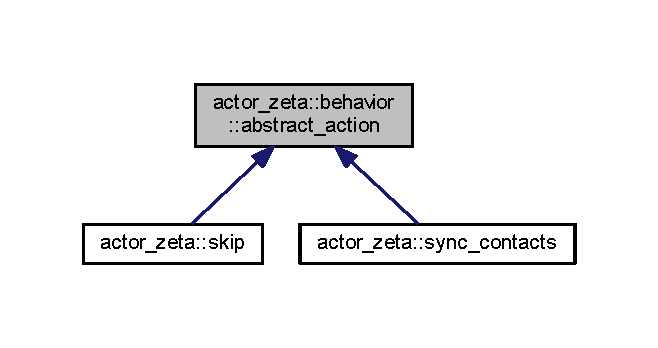
\includegraphics[width=316pt]{classactor__zeta_1_1behavior_1_1abstract__action__inherit__graph}
\end{center}
\end{figure}
\subsection*{Public Member Functions}
\begin{DoxyCompactItemize}
\item 
{\footnotesize template$<$std\+::size\+\_\+t N$>$ }\\\hyperlink{classactor__zeta_1_1behavior_1_1abstract__action_a510b0faad0820c2bfc66c8c17bb5c302}{abstract\+\_\+action} (const char(\&a\+Str)\mbox{[}N\mbox{]})
\item 
virtual \hyperlink{classactor__zeta_1_1behavior_1_1response}{response} $\ast$ \hyperlink{classactor__zeta_1_1behavior_1_1abstract__action_a5e48075d77fbd93615fc9b757e6a4d87}{operator()} (\hyperlink{classactor__zeta_1_1behavior_1_1request}{request} $\ast$)=0
\item 
auto \hyperlink{classactor__zeta_1_1behavior_1_1abstract__action_aa01dde89f5f3bc0a5b31e73eb5b38737}{name} () const -\/$>$ const \hyperlink{classactor__zeta_1_1behavior_1_1type__action}{type\+\_\+action} \&
\item 
virtual \hyperlink{classactor__zeta_1_1behavior_1_1abstract__action_a0a138630b650422e1e769a0ae10a681f}{$\sim$abstract\+\_\+action} ()=default
\end{DoxyCompactItemize}


\subsection{Detailed Description}
abstract concept of an action 

\subsection{Constructor \& Destructor Documentation}
\mbox{\Hypertarget{classactor__zeta_1_1behavior_1_1abstract__action_a510b0faad0820c2bfc66c8c17bb5c302}\label{classactor__zeta_1_1behavior_1_1abstract__action_a510b0faad0820c2bfc66c8c17bb5c302}} 
\index{actor\+\_\+zeta\+::behavior\+::abstract\+\_\+action@{actor\+\_\+zeta\+::behavior\+::abstract\+\_\+action}!abstract\+\_\+action@{abstract\+\_\+action}}
\index{abstract\+\_\+action@{abstract\+\_\+action}!actor\+\_\+zeta\+::behavior\+::abstract\+\_\+action@{actor\+\_\+zeta\+::behavior\+::abstract\+\_\+action}}
\subsubsection{\texorpdfstring{abstract\+\_\+action()}{abstract\_action()}}
{\footnotesize\ttfamily template$<$std\+::size\+\_\+t N$>$ \\
actor\+\_\+zeta\+::behavior\+::abstract\+\_\+action\+::abstract\+\_\+action (\begin{DoxyParamCaption}\item[{const char(\&)}]{a\+Str\mbox{[}\+N\mbox{]} }\end{DoxyParamCaption})\hspace{0.3cm}{\ttfamily [inline]}}

\mbox{\Hypertarget{classactor__zeta_1_1behavior_1_1abstract__action_a0a138630b650422e1e769a0ae10a681f}\label{classactor__zeta_1_1behavior_1_1abstract__action_a0a138630b650422e1e769a0ae10a681f}} 
\index{actor\+\_\+zeta\+::behavior\+::abstract\+\_\+action@{actor\+\_\+zeta\+::behavior\+::abstract\+\_\+action}!````~abstract\+\_\+action@{$\sim$abstract\+\_\+action}}
\index{````~abstract\+\_\+action@{$\sim$abstract\+\_\+action}!actor\+\_\+zeta\+::behavior\+::abstract\+\_\+action@{actor\+\_\+zeta\+::behavior\+::abstract\+\_\+action}}
\subsubsection{\texorpdfstring{$\sim$abstract\+\_\+action()}{~abstract\_action()}}
{\footnotesize\ttfamily virtual actor\+\_\+zeta\+::behavior\+::abstract\+\_\+action\+::$\sim$abstract\+\_\+action (\begin{DoxyParamCaption}{ }\end{DoxyParamCaption})\hspace{0.3cm}{\ttfamily [virtual]}, {\ttfamily [default]}}



\subsection{Member Function Documentation}
\mbox{\Hypertarget{classactor__zeta_1_1behavior_1_1abstract__action_aa01dde89f5f3bc0a5b31e73eb5b38737}\label{classactor__zeta_1_1behavior_1_1abstract__action_aa01dde89f5f3bc0a5b31e73eb5b38737}} 
\index{actor\+\_\+zeta\+::behavior\+::abstract\+\_\+action@{actor\+\_\+zeta\+::behavior\+::abstract\+\_\+action}!name@{name}}
\index{name@{name}!actor\+\_\+zeta\+::behavior\+::abstract\+\_\+action@{actor\+\_\+zeta\+::behavior\+::abstract\+\_\+action}}
\subsubsection{\texorpdfstring{name()}{name()}}
{\footnotesize\ttfamily auto actor\+\_\+zeta\+::behavior\+::abstract\+\_\+action\+::name (\begin{DoxyParamCaption}{ }\end{DoxyParamCaption}) const -\/$>$ const \hyperlink{classactor__zeta_1_1behavior_1_1type__action}{type\+\_\+action} \& \hspace{0.3cm}{\ttfamily [inline]}}

\mbox{\Hypertarget{classactor__zeta_1_1behavior_1_1abstract__action_a5e48075d77fbd93615fc9b757e6a4d87}\label{classactor__zeta_1_1behavior_1_1abstract__action_a5e48075d77fbd93615fc9b757e6a4d87}} 
\index{actor\+\_\+zeta\+::behavior\+::abstract\+\_\+action@{actor\+\_\+zeta\+::behavior\+::abstract\+\_\+action}!operator()@{operator()}}
\index{operator()@{operator()}!actor\+\_\+zeta\+::behavior\+::abstract\+\_\+action@{actor\+\_\+zeta\+::behavior\+::abstract\+\_\+action}}
\subsubsection{\texorpdfstring{operator()()}{operator()()}}
{\footnotesize\ttfamily virtual \hyperlink{classactor__zeta_1_1behavior_1_1response}{response}$\ast$ actor\+\_\+zeta\+::behavior\+::abstract\+\_\+action\+::operator() (\begin{DoxyParamCaption}\item[{\hyperlink{classactor__zeta_1_1behavior_1_1request}{request} $\ast$}]{ }\end{DoxyParamCaption})\hspace{0.3cm}{\ttfamily [pure virtual]}}



Implemented in \hyperlink{classactor__zeta_1_1sync__contacts_ab135afb3284f42dc36d54ea73a8b5ac8}{actor\+\_\+zeta\+::sync\+\_\+contacts}, and \hyperlink{classactor__zeta_1_1skip_a0a674c6ce55d365b2bae8ec19a58e29f}{actor\+\_\+zeta\+::skip}.



The documentation for this class was generated from the following file\+:\begin{DoxyCompactItemize}
\item 
\hyperlink{abstract__action_8hpp}{abstract\+\_\+action.\+hpp}\end{DoxyCompactItemize}

\hypertarget{classactor__zeta_1_1actor_1_1abstract__actor}{}\section{actor\+\_\+zeta\+:\+:actor\+:\+:abstract\+\_\+actor Class Reference}
\label{classactor__zeta_1_1actor_1_1abstract__actor}\index{actor\+\_\+zeta\+::actor\+::abstract\+\_\+actor@{actor\+\_\+zeta\+::actor\+::abstract\+\_\+actor}}


abstract concept of an actor  




{\ttfamily \#include $<$abstract\+\_\+actor.\+hpp$>$}



Inheritance diagram for actor\+\_\+zeta\+:\+:actor\+:\+:abstract\+\_\+actor\+:\nopagebreak
\begin{figure}[H]
\begin{center}
\leavevmode
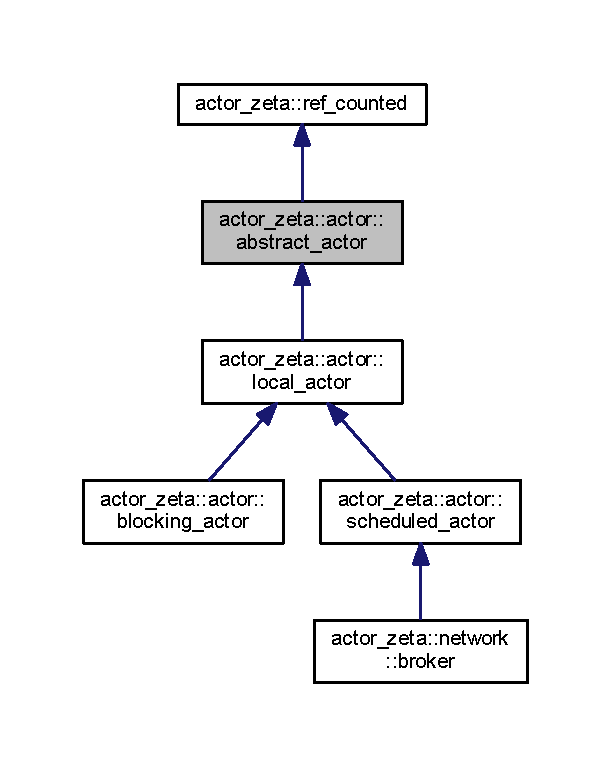
\includegraphics[width=293pt]{classactor__zeta_1_1actor_1_1abstract__actor__inherit__graph}
\end{center}
\end{figure}


Collaboration diagram for actor\+\_\+zeta\+:\+:actor\+:\+:abstract\+\_\+actor\+:\nopagebreak
\begin{figure}[H]
\begin{center}
\leavevmode
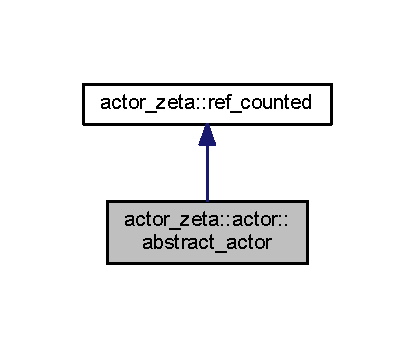
\includegraphics[width=199pt]{classactor__zeta_1_1actor_1_1abstract__actor__coll__graph}
\end{center}
\end{figure}
\subsection*{Public Member Functions}
\begin{DoxyCompactItemize}
\item 
const std\+::string \& \hyperlink{classactor__zeta_1_1actor_1_1abstract__actor_abebf7096ab054eb2be64151f589d70d7}{type} () const
\item 
virtual bool \hyperlink{classactor__zeta_1_1actor_1_1abstract__actor_a9316a5088e53255d74ade831e1fcfb47}{send} (\hyperlink{classactor__zeta_1_1messaging_1_1message}{messaging\+::message} $\ast$)=0
\item 
virtual bool \hyperlink{classactor__zeta_1_1actor_1_1abstract__actor_a929d99bea25095035695bad6e6516575}{send} (\hyperlink{classactor__zeta_1_1messaging_1_1message}{messaging\+::message} $\ast$, \hyperlink{structactor__zeta_1_1executor_1_1execution__device}{executor\+::execution\+\_\+device} $\ast$)=0
\item 
virtual \hyperlink{classactor__zeta_1_1actor_1_1abstract__actor_a12ab33a0d9267d3cf76bf3b2d5879c10}{$\sim$abstract\+\_\+actor} ()
\item 
\hyperlink{classactor__zeta_1_1actor_1_1actor__address}{actor\+\_\+address} \hyperlink{classactor__zeta_1_1actor_1_1abstract__actor_ae6b1f90ca34706d86d39b77c9cdd5a6f}{address} () const noexcept
\item 
\hyperlink{classactor__zeta_1_1environment_1_1environment}{environment\+::environment} $\ast$ \hyperlink{classactor__zeta_1_1actor_1_1abstract__actor_a4486fb3a9d042b2ec94aa1843db278d1}{env} () const
\end{DoxyCompactItemize}
\subsection*{Protected Member Functions}
\begin{DoxyCompactItemize}
\item 
\hyperlink{classactor__zeta_1_1actor_1_1abstract__actor_a65e0e2a223dc06413795f84747bd06b7}{abstract\+\_\+actor} (\hyperlink{classactor__zeta_1_1environment_1_1environment}{environment\+::environment} $\ast$, const std\+::string \&)
\end{DoxyCompactItemize}
\subsection*{Additional Inherited Members}


\subsection{Detailed Description}
abstract concept of an actor 

\subsection{Constructor \& Destructor Documentation}
\mbox{\Hypertarget{classactor__zeta_1_1actor_1_1abstract__actor_a12ab33a0d9267d3cf76bf3b2d5879c10}\label{classactor__zeta_1_1actor_1_1abstract__actor_a12ab33a0d9267d3cf76bf3b2d5879c10}} 
\index{actor\+\_\+zeta\+::actor\+::abstract\+\_\+actor@{actor\+\_\+zeta\+::actor\+::abstract\+\_\+actor}!````~abstract\+\_\+actor@{$\sim$abstract\+\_\+actor}}
\index{````~abstract\+\_\+actor@{$\sim$abstract\+\_\+actor}!actor\+\_\+zeta\+::actor\+::abstract\+\_\+actor@{actor\+\_\+zeta\+::actor\+::abstract\+\_\+actor}}
\subsubsection{\texorpdfstring{$\sim$abstract\+\_\+actor()}{~abstract\_actor()}}
{\footnotesize\ttfamily virtual actor\+\_\+zeta\+::actor\+::abstract\+\_\+actor\+::$\sim$abstract\+\_\+actor (\begin{DoxyParamCaption}{ }\end{DoxyParamCaption})\hspace{0.3cm}{\ttfamily [inline]}, {\ttfamily [virtual]}}

\mbox{\Hypertarget{classactor__zeta_1_1actor_1_1abstract__actor_a65e0e2a223dc06413795f84747bd06b7}\label{classactor__zeta_1_1actor_1_1abstract__actor_a65e0e2a223dc06413795f84747bd06b7}} 
\index{actor\+\_\+zeta\+::actor\+::abstract\+\_\+actor@{actor\+\_\+zeta\+::actor\+::abstract\+\_\+actor}!abstract\+\_\+actor@{abstract\+\_\+actor}}
\index{abstract\+\_\+actor@{abstract\+\_\+actor}!actor\+\_\+zeta\+::actor\+::abstract\+\_\+actor@{actor\+\_\+zeta\+::actor\+::abstract\+\_\+actor}}
\subsubsection{\texorpdfstring{abstract\+\_\+actor()}{abstract\_actor()}}
{\footnotesize\ttfamily actor\+\_\+zeta\+::actor\+::abstract\+\_\+actor\+::abstract\+\_\+actor (\begin{DoxyParamCaption}\item[{\hyperlink{classactor__zeta_1_1environment_1_1environment}{environment\+::environment} $\ast$}]{env,  }\item[{const std\+::string \&}]{type }\end{DoxyParamCaption})\hspace{0.3cm}{\ttfamily [protected]}}



\subsection{Member Function Documentation}
\mbox{\Hypertarget{classactor__zeta_1_1actor_1_1abstract__actor_ae6b1f90ca34706d86d39b77c9cdd5a6f}\label{classactor__zeta_1_1actor_1_1abstract__actor_ae6b1f90ca34706d86d39b77c9cdd5a6f}} 
\index{actor\+\_\+zeta\+::actor\+::abstract\+\_\+actor@{actor\+\_\+zeta\+::actor\+::abstract\+\_\+actor}!address@{address}}
\index{address@{address}!actor\+\_\+zeta\+::actor\+::abstract\+\_\+actor@{actor\+\_\+zeta\+::actor\+::abstract\+\_\+actor}}
\subsubsection{\texorpdfstring{address()}{address()}}
{\footnotesize\ttfamily \hyperlink{classactor__zeta_1_1actor_1_1actor__address}{actor\+\_\+address} actor\+\_\+zeta\+::actor\+::abstract\+\_\+actor\+::address (\begin{DoxyParamCaption}{ }\end{DoxyParamCaption}) const\hspace{0.3cm}{\ttfamily [noexcept]}}

\mbox{\Hypertarget{classactor__zeta_1_1actor_1_1abstract__actor_a4486fb3a9d042b2ec94aa1843db278d1}\label{classactor__zeta_1_1actor_1_1abstract__actor_a4486fb3a9d042b2ec94aa1843db278d1}} 
\index{actor\+\_\+zeta\+::actor\+::abstract\+\_\+actor@{actor\+\_\+zeta\+::actor\+::abstract\+\_\+actor}!env@{env}}
\index{env@{env}!actor\+\_\+zeta\+::actor\+::abstract\+\_\+actor@{actor\+\_\+zeta\+::actor\+::abstract\+\_\+actor}}
\subsubsection{\texorpdfstring{env()}{env()}}
{\footnotesize\ttfamily \hyperlink{classactor__zeta_1_1environment_1_1environment}{environment\+::environment} $\ast$ actor\+\_\+zeta\+::actor\+::abstract\+\_\+actor\+::env (\begin{DoxyParamCaption}{ }\end{DoxyParamCaption}) const}

\mbox{\Hypertarget{classactor__zeta_1_1actor_1_1abstract__actor_a9316a5088e53255d74ade831e1fcfb47}\label{classactor__zeta_1_1actor_1_1abstract__actor_a9316a5088e53255d74ade831e1fcfb47}} 
\index{actor\+\_\+zeta\+::actor\+::abstract\+\_\+actor@{actor\+\_\+zeta\+::actor\+::abstract\+\_\+actor}!send@{send}}
\index{send@{send}!actor\+\_\+zeta\+::actor\+::abstract\+\_\+actor@{actor\+\_\+zeta\+::actor\+::abstract\+\_\+actor}}
\subsubsection{\texorpdfstring{send()}{send()}\hspace{0.1cm}{\footnotesize\ttfamily [1/2]}}
{\footnotesize\ttfamily virtual bool actor\+\_\+zeta\+::actor\+::abstract\+\_\+actor\+::send (\begin{DoxyParamCaption}\item[{\hyperlink{classactor__zeta_1_1messaging_1_1message}{messaging\+::message} $\ast$}]{ }\end{DoxyParamCaption})\hspace{0.3cm}{\ttfamily [pure virtual]}}



Implemented in \hyperlink{classactor__zeta_1_1actor_1_1scheduled__actor_acdd757f48a5233a9914209aaf7a2b5ed}{actor\+\_\+zeta\+::actor\+::scheduled\+\_\+actor}.

\mbox{\Hypertarget{classactor__zeta_1_1actor_1_1abstract__actor_a929d99bea25095035695bad6e6516575}\label{classactor__zeta_1_1actor_1_1abstract__actor_a929d99bea25095035695bad6e6516575}} 
\index{actor\+\_\+zeta\+::actor\+::abstract\+\_\+actor@{actor\+\_\+zeta\+::actor\+::abstract\+\_\+actor}!send@{send}}
\index{send@{send}!actor\+\_\+zeta\+::actor\+::abstract\+\_\+actor@{actor\+\_\+zeta\+::actor\+::abstract\+\_\+actor}}
\subsubsection{\texorpdfstring{send()}{send()}\hspace{0.1cm}{\footnotesize\ttfamily [2/2]}}
{\footnotesize\ttfamily virtual bool actor\+\_\+zeta\+::actor\+::abstract\+\_\+actor\+::send (\begin{DoxyParamCaption}\item[{\hyperlink{classactor__zeta_1_1messaging_1_1message}{messaging\+::message} $\ast$}]{,  }\item[{\hyperlink{structactor__zeta_1_1executor_1_1execution__device}{executor\+::execution\+\_\+device} $\ast$}]{ }\end{DoxyParamCaption})\hspace{0.3cm}{\ttfamily [pure virtual]}}



Implemented in \hyperlink{classactor__zeta_1_1actor_1_1scheduled__actor_a223d20f327713fa65968f909aacb0a32}{actor\+\_\+zeta\+::actor\+::scheduled\+\_\+actor}.

\mbox{\Hypertarget{classactor__zeta_1_1actor_1_1abstract__actor_abebf7096ab054eb2be64151f589d70d7}\label{classactor__zeta_1_1actor_1_1abstract__actor_abebf7096ab054eb2be64151f589d70d7}} 
\index{actor\+\_\+zeta\+::actor\+::abstract\+\_\+actor@{actor\+\_\+zeta\+::actor\+::abstract\+\_\+actor}!type@{type}}
\index{type@{type}!actor\+\_\+zeta\+::actor\+::abstract\+\_\+actor@{actor\+\_\+zeta\+::actor\+::abstract\+\_\+actor}}
\subsubsection{\texorpdfstring{type()}{type()}}
{\footnotesize\ttfamily const std\+::string \& actor\+\_\+zeta\+::actor\+::abstract\+\_\+actor\+::type (\begin{DoxyParamCaption}{ }\end{DoxyParamCaption}) const}



The documentation for this class was generated from the following files\+:\begin{DoxyCompactItemize}
\item 
\hyperlink{abstract__actor_8hpp}{abstract\+\_\+actor.\+hpp}\item 
\hyperlink{abstract__actor_8cpp}{abstract\+\_\+actor.\+cpp}\end{DoxyCompactItemize}

\hypertarget{classactor__zeta_1_1executor_1_1abstract__coordinator}{}\section{actor\+\_\+zeta\+:\+:executor\+:\+:abstract\+\_\+coordinator Class Reference}
\label{classactor__zeta_1_1executor_1_1abstract__coordinator}\index{actor\+\_\+zeta\+::executor\+::abstract\+\_\+coordinator@{actor\+\_\+zeta\+::executor\+::abstract\+\_\+coordinator}}


abstract concept of an coordination approach  




{\ttfamily \#include $<$abstract\+\_\+coordinator.\+hpp$>$}



Inheritance diagram for actor\+\_\+zeta\+:\+:executor\+:\+:abstract\+\_\+coordinator\+:\nopagebreak
\begin{figure}[H]
\begin{center}
\leavevmode
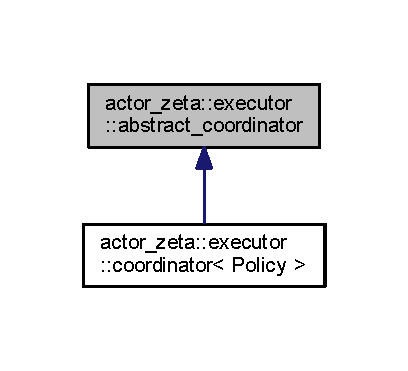
\includegraphics[width=196pt]{classactor__zeta_1_1executor_1_1abstract__coordinator__inherit__graph}
\end{center}
\end{figure}
\subsection*{Public Member Functions}
\begin{DoxyCompactItemize}
\item 
virtual void \hyperlink{classactor__zeta_1_1executor_1_1abstract__coordinator_a4e9c6ebc0d950993e051a6f512539dfa}{submit} (\hyperlink{structactor__zeta_1_1executor_1_1executable}{executable} $\ast$)=0
\item 
virtual void \hyperlink{classactor__zeta_1_1executor_1_1abstract__coordinator_abbbe1a84649a3ae2cfcb60c7728b2944}{start} ()=0
\item 
virtual \hyperlink{classactor__zeta_1_1executor_1_1abstract__coordinator_a3168a7bb00a6499f2ec0ab33e7682fd1}{$\sim$abstract\+\_\+coordinator} ()=default
\item 
\hyperlink{classactor__zeta_1_1executor_1_1abstract__coordinator_a52f408cbdd6b33f33a02eb3b288c9247}{abstract\+\_\+coordinator} (size\+\_\+t num\+\_\+worker\+\_\+threads, size\+\_\+t max\+\_\+throughput\+\_\+param)
\item 
size\+\_\+t \hyperlink{classactor__zeta_1_1executor_1_1abstract__coordinator_aeb428a4c165e5d01ff7e7c93d9404d11}{max\+\_\+throughput} () const
\item 
size\+\_\+t \hyperlink{classactor__zeta_1_1executor_1_1abstract__coordinator_a50c97e6b0508fe609e0ca62a7da3ee96}{num\+\_\+workers} () const
\end{DoxyCompactItemize}


\subsection{Detailed Description}
abstract concept of an coordination approach 

\subsection{Constructor \& Destructor Documentation}
\mbox{\Hypertarget{classactor__zeta_1_1executor_1_1abstract__coordinator_a3168a7bb00a6499f2ec0ab33e7682fd1}\label{classactor__zeta_1_1executor_1_1abstract__coordinator_a3168a7bb00a6499f2ec0ab33e7682fd1}} 
\index{actor\+\_\+zeta\+::executor\+::abstract\+\_\+coordinator@{actor\+\_\+zeta\+::executor\+::abstract\+\_\+coordinator}!````~abstract\+\_\+coordinator@{$\sim$abstract\+\_\+coordinator}}
\index{````~abstract\+\_\+coordinator@{$\sim$abstract\+\_\+coordinator}!actor\+\_\+zeta\+::executor\+::abstract\+\_\+coordinator@{actor\+\_\+zeta\+::executor\+::abstract\+\_\+coordinator}}
\subsubsection{\texorpdfstring{$\sim$abstract\+\_\+coordinator()}{~abstract\_coordinator()}}
{\footnotesize\ttfamily virtual actor\+\_\+zeta\+::executor\+::abstract\+\_\+coordinator\+::$\sim$abstract\+\_\+coordinator (\begin{DoxyParamCaption}{ }\end{DoxyParamCaption})\hspace{0.3cm}{\ttfamily [virtual]}, {\ttfamily [default]}}

\mbox{\Hypertarget{classactor__zeta_1_1executor_1_1abstract__coordinator_a52f408cbdd6b33f33a02eb3b288c9247}\label{classactor__zeta_1_1executor_1_1abstract__coordinator_a52f408cbdd6b33f33a02eb3b288c9247}} 
\index{actor\+\_\+zeta\+::executor\+::abstract\+\_\+coordinator@{actor\+\_\+zeta\+::executor\+::abstract\+\_\+coordinator}!abstract\+\_\+coordinator@{abstract\+\_\+coordinator}}
\index{abstract\+\_\+coordinator@{abstract\+\_\+coordinator}!actor\+\_\+zeta\+::executor\+::abstract\+\_\+coordinator@{actor\+\_\+zeta\+::executor\+::abstract\+\_\+coordinator}}
\subsubsection{\texorpdfstring{abstract\+\_\+coordinator()}{abstract\_coordinator()}}
{\footnotesize\ttfamily actor\+\_\+zeta\+::executor\+::abstract\+\_\+coordinator\+::abstract\+\_\+coordinator (\begin{DoxyParamCaption}\item[{size\+\_\+t}]{num\+\_\+worker\+\_\+threads,  }\item[{size\+\_\+t}]{max\+\_\+throughput\+\_\+param }\end{DoxyParamCaption})\hspace{0.3cm}{\ttfamily [inline]}, {\ttfamily [explicit]}}



\subsection{Member Function Documentation}
\mbox{\Hypertarget{classactor__zeta_1_1executor_1_1abstract__coordinator_aeb428a4c165e5d01ff7e7c93d9404d11}\label{classactor__zeta_1_1executor_1_1abstract__coordinator_aeb428a4c165e5d01ff7e7c93d9404d11}} 
\index{actor\+\_\+zeta\+::executor\+::abstract\+\_\+coordinator@{actor\+\_\+zeta\+::executor\+::abstract\+\_\+coordinator}!max\+\_\+throughput@{max\+\_\+throughput}}
\index{max\+\_\+throughput@{max\+\_\+throughput}!actor\+\_\+zeta\+::executor\+::abstract\+\_\+coordinator@{actor\+\_\+zeta\+::executor\+::abstract\+\_\+coordinator}}
\subsubsection{\texorpdfstring{max\+\_\+throughput()}{max\_throughput()}}
{\footnotesize\ttfamily size\+\_\+t actor\+\_\+zeta\+::executor\+::abstract\+\_\+coordinator\+::max\+\_\+throughput (\begin{DoxyParamCaption}{ }\end{DoxyParamCaption}) const\hspace{0.3cm}{\ttfamily [inline]}}

\mbox{\Hypertarget{classactor__zeta_1_1executor_1_1abstract__coordinator_a50c97e6b0508fe609e0ca62a7da3ee96}\label{classactor__zeta_1_1executor_1_1abstract__coordinator_a50c97e6b0508fe609e0ca62a7da3ee96}} 
\index{actor\+\_\+zeta\+::executor\+::abstract\+\_\+coordinator@{actor\+\_\+zeta\+::executor\+::abstract\+\_\+coordinator}!num\+\_\+workers@{num\+\_\+workers}}
\index{num\+\_\+workers@{num\+\_\+workers}!actor\+\_\+zeta\+::executor\+::abstract\+\_\+coordinator@{actor\+\_\+zeta\+::executor\+::abstract\+\_\+coordinator}}
\subsubsection{\texorpdfstring{num\+\_\+workers()}{num\_workers()}}
{\footnotesize\ttfamily size\+\_\+t actor\+\_\+zeta\+::executor\+::abstract\+\_\+coordinator\+::num\+\_\+workers (\begin{DoxyParamCaption}{ }\end{DoxyParamCaption}) const\hspace{0.3cm}{\ttfamily [inline]}}

\mbox{\Hypertarget{classactor__zeta_1_1executor_1_1abstract__coordinator_abbbe1a84649a3ae2cfcb60c7728b2944}\label{classactor__zeta_1_1executor_1_1abstract__coordinator_abbbe1a84649a3ae2cfcb60c7728b2944}} 
\index{actor\+\_\+zeta\+::executor\+::abstract\+\_\+coordinator@{actor\+\_\+zeta\+::executor\+::abstract\+\_\+coordinator}!start@{start}}
\index{start@{start}!actor\+\_\+zeta\+::executor\+::abstract\+\_\+coordinator@{actor\+\_\+zeta\+::executor\+::abstract\+\_\+coordinator}}
\subsubsection{\texorpdfstring{start()}{start()}}
{\footnotesize\ttfamily virtual void actor\+\_\+zeta\+::executor\+::abstract\+\_\+coordinator\+::start (\begin{DoxyParamCaption}{ }\end{DoxyParamCaption})\hspace{0.3cm}{\ttfamily [pure virtual]}}



Implemented in \hyperlink{classactor__zeta_1_1executor_1_1coordinator_a1b73b7ddd6b48ba3e15b6f710cb21808}{actor\+\_\+zeta\+::executor\+::coordinator$<$ Policy $>$}.

\mbox{\Hypertarget{classactor__zeta_1_1executor_1_1abstract__coordinator_a4e9c6ebc0d950993e051a6f512539dfa}\label{classactor__zeta_1_1executor_1_1abstract__coordinator_a4e9c6ebc0d950993e051a6f512539dfa}} 
\index{actor\+\_\+zeta\+::executor\+::abstract\+\_\+coordinator@{actor\+\_\+zeta\+::executor\+::abstract\+\_\+coordinator}!submit@{submit}}
\index{submit@{submit}!actor\+\_\+zeta\+::executor\+::abstract\+\_\+coordinator@{actor\+\_\+zeta\+::executor\+::abstract\+\_\+coordinator}}
\subsubsection{\texorpdfstring{submit()}{submit()}}
{\footnotesize\ttfamily virtual void actor\+\_\+zeta\+::executor\+::abstract\+\_\+coordinator\+::submit (\begin{DoxyParamCaption}\item[{\hyperlink{structactor__zeta_1_1executor_1_1executable}{executable} $\ast$}]{ }\end{DoxyParamCaption})\hspace{0.3cm}{\ttfamily [pure virtual]}}



The documentation for this class was generated from the following file\+:\begin{DoxyCompactItemize}
\item 
\hyperlink{abstract__coordinator_8hpp}{abstract\+\_\+coordinator.\+hpp}\end{DoxyCompactItemize}

\hypertarget{classactor__zeta_1_1behavior_1_1action}{}\section{actor\+\_\+zeta\+:\+:behavior\+:\+:action Class Reference}
\label{classactor__zeta_1_1behavior_1_1action}\index{actor\+\_\+zeta\+::behavior\+::action@{actor\+\_\+zeta\+::behavior\+::action}}


Basic action implementation.  




{\ttfamily \#include $<$action.\+hpp$>$}

\subsection*{Public Member Functions}
\begin{DoxyCompactItemize}
\item 
\hyperlink{classactor__zeta_1_1behavior_1_1action_ae51e1d01deb04289074554b63a58173c}{action} ()=default
\item 
\hyperlink{classactor__zeta_1_1behavior_1_1action_a5aee8f55bd72c023101cfdc15743f9a3}{action} (const \hyperlink{classactor__zeta_1_1behavior_1_1action}{action} \&)=delete
\item 
\hyperlink{classactor__zeta_1_1behavior_1_1action}{action} \& \hyperlink{classactor__zeta_1_1behavior_1_1action_aa9055a54598dce71608fb023cfd4c37a}{operator=} (const \hyperlink{classactor__zeta_1_1behavior_1_1action}{action} \&)=delete
\item 
\hyperlink{classactor__zeta_1_1behavior_1_1action_a08d5d3dbb99797ed51ec40a1c9c2331f}{action} (\hyperlink{classactor__zeta_1_1behavior_1_1action}{action} \&\&)=default
\item 
\hyperlink{classactor__zeta_1_1behavior_1_1action}{action} \& \hyperlink{classactor__zeta_1_1behavior_1_1action_a32a15f7c6e38ffa311303dc6ff2d8bc2}{operator=} (\hyperlink{classactor__zeta_1_1behavior_1_1action}{action} \&\&)=default
\item 
\hyperlink{classactor__zeta_1_1behavior_1_1action_aca4d1f16a134e04a5812f3d44e17aa9c}{$\sim$action} ()=default
\item 
\hyperlink{classactor__zeta_1_1behavior_1_1action_a154dc8a6ec5b329fbc13df04dbc9df1b}{action} (\hyperlink{classactor__zeta_1_1behavior_1_1abstract__action}{abstract\+\_\+action} $\ast$)
\item 
\hyperlink{classactor__zeta_1_1behavior_1_1response}{response} $\ast$ \hyperlink{classactor__zeta_1_1behavior_1_1action_a5d46cfac3fb311555544971809d1c60c}{operator()} (\hyperlink{classactor__zeta_1_1behavior_1_1request}{request} $\ast$)
\end{DoxyCompactItemize}


\subsection{Detailed Description}
Basic action implementation. 

\subsection{Constructor \& Destructor Documentation}
\mbox{\Hypertarget{classactor__zeta_1_1behavior_1_1action_ae51e1d01deb04289074554b63a58173c}\label{classactor__zeta_1_1behavior_1_1action_ae51e1d01deb04289074554b63a58173c}} 
\index{actor\+\_\+zeta\+::behavior\+::action@{actor\+\_\+zeta\+::behavior\+::action}!action@{action}}
\index{action@{action}!actor\+\_\+zeta\+::behavior\+::action@{actor\+\_\+zeta\+::behavior\+::action}}
\subsubsection{\texorpdfstring{action()}{action()}\hspace{0.1cm}{\footnotesize\ttfamily [1/4]}}
{\footnotesize\ttfamily actor\+\_\+zeta\+::behavior\+::action\+::action (\begin{DoxyParamCaption}{ }\end{DoxyParamCaption})\hspace{0.3cm}{\ttfamily [default]}}

\mbox{\Hypertarget{classactor__zeta_1_1behavior_1_1action_a5aee8f55bd72c023101cfdc15743f9a3}\label{classactor__zeta_1_1behavior_1_1action_a5aee8f55bd72c023101cfdc15743f9a3}} 
\index{actor\+\_\+zeta\+::behavior\+::action@{actor\+\_\+zeta\+::behavior\+::action}!action@{action}}
\index{action@{action}!actor\+\_\+zeta\+::behavior\+::action@{actor\+\_\+zeta\+::behavior\+::action}}
\subsubsection{\texorpdfstring{action()}{action()}\hspace{0.1cm}{\footnotesize\ttfamily [2/4]}}
{\footnotesize\ttfamily actor\+\_\+zeta\+::behavior\+::action\+::action (\begin{DoxyParamCaption}\item[{const \hyperlink{classactor__zeta_1_1behavior_1_1action}{action} \&}]{ }\end{DoxyParamCaption})\hspace{0.3cm}{\ttfamily [delete]}}

\mbox{\Hypertarget{classactor__zeta_1_1behavior_1_1action_a08d5d3dbb99797ed51ec40a1c9c2331f}\label{classactor__zeta_1_1behavior_1_1action_a08d5d3dbb99797ed51ec40a1c9c2331f}} 
\index{actor\+\_\+zeta\+::behavior\+::action@{actor\+\_\+zeta\+::behavior\+::action}!action@{action}}
\index{action@{action}!actor\+\_\+zeta\+::behavior\+::action@{actor\+\_\+zeta\+::behavior\+::action}}
\subsubsection{\texorpdfstring{action()}{action()}\hspace{0.1cm}{\footnotesize\ttfamily [3/4]}}
{\footnotesize\ttfamily actor\+\_\+zeta\+::behavior\+::action\+::action (\begin{DoxyParamCaption}\item[{\hyperlink{classactor__zeta_1_1behavior_1_1action}{action} \&\&}]{ }\end{DoxyParamCaption})\hspace{0.3cm}{\ttfamily [default]}}

\mbox{\Hypertarget{classactor__zeta_1_1behavior_1_1action_aca4d1f16a134e04a5812f3d44e17aa9c}\label{classactor__zeta_1_1behavior_1_1action_aca4d1f16a134e04a5812f3d44e17aa9c}} 
\index{actor\+\_\+zeta\+::behavior\+::action@{actor\+\_\+zeta\+::behavior\+::action}!````~action@{$\sim$action}}
\index{````~action@{$\sim$action}!actor\+\_\+zeta\+::behavior\+::action@{actor\+\_\+zeta\+::behavior\+::action}}
\subsubsection{\texorpdfstring{$\sim$action()}{~action()}}
{\footnotesize\ttfamily actor\+\_\+zeta\+::behavior\+::action\+::$\sim$action (\begin{DoxyParamCaption}{ }\end{DoxyParamCaption})\hspace{0.3cm}{\ttfamily [default]}}

\mbox{\Hypertarget{classactor__zeta_1_1behavior_1_1action_a154dc8a6ec5b329fbc13df04dbc9df1b}\label{classactor__zeta_1_1behavior_1_1action_a154dc8a6ec5b329fbc13df04dbc9df1b}} 
\index{actor\+\_\+zeta\+::behavior\+::action@{actor\+\_\+zeta\+::behavior\+::action}!action@{action}}
\index{action@{action}!actor\+\_\+zeta\+::behavior\+::action@{actor\+\_\+zeta\+::behavior\+::action}}
\subsubsection{\texorpdfstring{action()}{action()}\hspace{0.1cm}{\footnotesize\ttfamily [4/4]}}
{\footnotesize\ttfamily actor\+\_\+zeta\+::behavior\+::action\+::action (\begin{DoxyParamCaption}\item[{\hyperlink{classactor__zeta_1_1behavior_1_1abstract__action}{abstract\+\_\+action} $\ast$}]{aa }\end{DoxyParamCaption})\hspace{0.3cm}{\ttfamily [explicit]}}



\subsection{Member Function Documentation}
\mbox{\Hypertarget{classactor__zeta_1_1behavior_1_1action_a5d46cfac3fb311555544971809d1c60c}\label{classactor__zeta_1_1behavior_1_1action_a5d46cfac3fb311555544971809d1c60c}} 
\index{actor\+\_\+zeta\+::behavior\+::action@{actor\+\_\+zeta\+::behavior\+::action}!operator()@{operator()}}
\index{operator()@{operator()}!actor\+\_\+zeta\+::behavior\+::action@{actor\+\_\+zeta\+::behavior\+::action}}
\subsubsection{\texorpdfstring{operator()()}{operator()()}}
{\footnotesize\ttfamily \hyperlink{classactor__zeta_1_1behavior_1_1response}{response} $\ast$ actor\+\_\+zeta\+::behavior\+::action\+::operator() (\begin{DoxyParamCaption}\item[{\hyperlink{classactor__zeta_1_1behavior_1_1request}{request} $\ast$}]{request\+\_\+ }\end{DoxyParamCaption})}

\mbox{\Hypertarget{classactor__zeta_1_1behavior_1_1action_aa9055a54598dce71608fb023cfd4c37a}\label{classactor__zeta_1_1behavior_1_1action_aa9055a54598dce71608fb023cfd4c37a}} 
\index{actor\+\_\+zeta\+::behavior\+::action@{actor\+\_\+zeta\+::behavior\+::action}!operator=@{operator=}}
\index{operator=@{operator=}!actor\+\_\+zeta\+::behavior\+::action@{actor\+\_\+zeta\+::behavior\+::action}}
\subsubsection{\texorpdfstring{operator=()}{operator=()}\hspace{0.1cm}{\footnotesize\ttfamily [1/2]}}
{\footnotesize\ttfamily \hyperlink{classactor__zeta_1_1behavior_1_1action}{action}\& actor\+\_\+zeta\+::behavior\+::action\+::operator= (\begin{DoxyParamCaption}\item[{const \hyperlink{classactor__zeta_1_1behavior_1_1action}{action} \&}]{ }\end{DoxyParamCaption})\hspace{0.3cm}{\ttfamily [delete]}}

\mbox{\Hypertarget{classactor__zeta_1_1behavior_1_1action_a32a15f7c6e38ffa311303dc6ff2d8bc2}\label{classactor__zeta_1_1behavior_1_1action_a32a15f7c6e38ffa311303dc6ff2d8bc2}} 
\index{actor\+\_\+zeta\+::behavior\+::action@{actor\+\_\+zeta\+::behavior\+::action}!operator=@{operator=}}
\index{operator=@{operator=}!actor\+\_\+zeta\+::behavior\+::action@{actor\+\_\+zeta\+::behavior\+::action}}
\subsubsection{\texorpdfstring{operator=()}{operator=()}\hspace{0.1cm}{\footnotesize\ttfamily [2/2]}}
{\footnotesize\ttfamily \hyperlink{classactor__zeta_1_1behavior_1_1action}{action}\& actor\+\_\+zeta\+::behavior\+::action\+::operator= (\begin{DoxyParamCaption}\item[{\hyperlink{classactor__zeta_1_1behavior_1_1action}{action} \&\&}]{ }\end{DoxyParamCaption})\hspace{0.3cm}{\ttfamily [default]}}



The documentation for this class was generated from the following files\+:\begin{DoxyCompactItemize}
\item 
\hyperlink{action_8hpp}{action.\+hpp}\item 
\hyperlink{action_8cpp}{action.\+cpp}\end{DoxyCompactItemize}

\hypertarget{classactor__zeta_1_1actor_1_1actor}{}\section{actor\+\_\+zeta\+:\+:actor\+:\+:actor Class Reference}
\label{classactor__zeta_1_1actor_1_1actor}\index{actor\+\_\+zeta\+::actor\+::actor@{actor\+\_\+zeta\+::actor\+::actor}}


Basic actor implementation.  




{\ttfamily \#include $<$actor.\+hpp$>$}

\subsection*{Public Member Functions}
\begin{DoxyCompactItemize}
\item 
\hyperlink{classactor__zeta_1_1actor_1_1actor_a7ec6ba681de874c0ffc40f81706387ab}{actor} ()=default
\item 
\hyperlink{classactor__zeta_1_1actor_1_1actor_a56decfd3d1d91fdfc6179189a4f558b3}{actor} (const \hyperlink{classactor__zeta_1_1actor_1_1actor}{actor} \&a)=delete
\item 
\hyperlink{classactor__zeta_1_1actor_1_1actor_a9cfa98421bd8eed8fe16c7de6782622a}{actor} (\hyperlink{classactor__zeta_1_1actor_1_1actor}{actor} \&\&a)=default
\item 
\hyperlink{classactor__zeta_1_1actor_1_1actor}{actor} \& \hyperlink{classactor__zeta_1_1actor_1_1actor_a00a3e4d947b09fc376b69d2f122d46b9}{operator=} (const \hyperlink{classactor__zeta_1_1actor_1_1actor}{actor} \&a)=delete
\item 
\hyperlink{classactor__zeta_1_1actor_1_1actor}{actor} \& \hyperlink{classactor__zeta_1_1actor_1_1actor_a8b49fc68d207e728493643678abe5329}{operator=} (\hyperlink{classactor__zeta_1_1actor_1_1actor}{actor} \&\&a)=default
\item 
{\footnotesize template$<$class T $>$ }\\\hyperlink{classactor__zeta_1_1actor_1_1actor_a34cf041d9a42b0ec60a6021a9e5858fc}{actor} (\hyperlink{classactor__zeta_1_1intrusive__ptr}{intrusive\+\_\+ptr}$<$ T $>$ ptr)
\item 
{\footnotesize template$<$class T $>$ }\\\hyperlink{classactor__zeta_1_1actor_1_1actor_aac0d60ab708b9524c8cd1ca22060c8ad}{actor} (T $\ast$ptr)
\item 
{\footnotesize template$<$class T $>$ }\\\hyperlink{classactor__zeta_1_1actor_1_1actor}{actor} \& \hyperlink{classactor__zeta_1_1actor_1_1actor_aaa3ce62db27a8dbd20be3e2a1c997bff}{operator=} (\hyperlink{classactor__zeta_1_1intrusive__ptr}{intrusive\+\_\+ptr}$<$ T $>$ ptr)
\item 
{\footnotesize template$<$class T $>$ }\\\hyperlink{classactor__zeta_1_1actor_1_1actor}{actor} \& \hyperlink{classactor__zeta_1_1actor_1_1actor_a9573ab3ea73f292601ee7094ac63c37e}{operator=} (T $\ast$ptr)
\item 
\hyperlink{classactor__zeta_1_1actor_1_1actor__address}{actor\+\_\+address} \hyperlink{classactor__zeta_1_1actor_1_1actor_ad76c050fba9c3c212dd8ef7720012d91}{address} () const noexcept
\item 
\hyperlink{classactor__zeta_1_1actor_1_1actor_ac88a08ce8cb7657906aae1c63c010f8a}{$\sim$actor} ()
\item 
\hyperlink{classactor__zeta_1_1actor_1_1abstract__actor}{abstract\+\_\+actor} $\ast$ \hyperlink{classactor__zeta_1_1actor_1_1actor_a2321f0000f10f669cd60664bde0b7878}{operator-\/$>$} () const noexcept
\item 
\hyperlink{classactor__zeta_1_1actor_1_1actor_a0dd1822479e1f7793d113d93b08ac483}{operator bool} () const noexcept
\item 
const std\+::string \& \hyperlink{classactor__zeta_1_1actor_1_1actor_a6ea7c424ac30d951cd1a003d39e82755}{type} () const
\item 
bool \hyperlink{classactor__zeta_1_1actor_1_1actor_a161c252c7206ebb2a158cf552c098ec1}{operator!} () const noexcept
\end{DoxyCompactItemize}


\subsection{Detailed Description}
Basic actor implementation. 

\subsection{Constructor \& Destructor Documentation}
\mbox{\Hypertarget{classactor__zeta_1_1actor_1_1actor_a7ec6ba681de874c0ffc40f81706387ab}\label{classactor__zeta_1_1actor_1_1actor_a7ec6ba681de874c0ffc40f81706387ab}} 
\index{actor\+\_\+zeta\+::actor\+::actor@{actor\+\_\+zeta\+::actor\+::actor}!actor@{actor}}
\index{actor@{actor}!actor\+\_\+zeta\+::actor\+::actor@{actor\+\_\+zeta\+::actor\+::actor}}
\subsubsection{\texorpdfstring{actor()}{actor()}\hspace{0.1cm}{\footnotesize\ttfamily [1/5]}}
{\footnotesize\ttfamily actor\+\_\+zeta\+::actor\+::actor\+::actor (\begin{DoxyParamCaption}{ }\end{DoxyParamCaption})\hspace{0.3cm}{\ttfamily [default]}}

\mbox{\Hypertarget{classactor__zeta_1_1actor_1_1actor_a56decfd3d1d91fdfc6179189a4f558b3}\label{classactor__zeta_1_1actor_1_1actor_a56decfd3d1d91fdfc6179189a4f558b3}} 
\index{actor\+\_\+zeta\+::actor\+::actor@{actor\+\_\+zeta\+::actor\+::actor}!actor@{actor}}
\index{actor@{actor}!actor\+\_\+zeta\+::actor\+::actor@{actor\+\_\+zeta\+::actor\+::actor}}
\subsubsection{\texorpdfstring{actor()}{actor()}\hspace{0.1cm}{\footnotesize\ttfamily [2/5]}}
{\footnotesize\ttfamily actor\+\_\+zeta\+::actor\+::actor\+::actor (\begin{DoxyParamCaption}\item[{const \hyperlink{classactor__zeta_1_1actor_1_1actor}{actor} \&}]{a }\end{DoxyParamCaption})\hspace{0.3cm}{\ttfamily [delete]}}

\mbox{\Hypertarget{classactor__zeta_1_1actor_1_1actor_a9cfa98421bd8eed8fe16c7de6782622a}\label{classactor__zeta_1_1actor_1_1actor_a9cfa98421bd8eed8fe16c7de6782622a}} 
\index{actor\+\_\+zeta\+::actor\+::actor@{actor\+\_\+zeta\+::actor\+::actor}!actor@{actor}}
\index{actor@{actor}!actor\+\_\+zeta\+::actor\+::actor@{actor\+\_\+zeta\+::actor\+::actor}}
\subsubsection{\texorpdfstring{actor()}{actor()}\hspace{0.1cm}{\footnotesize\ttfamily [3/5]}}
{\footnotesize\ttfamily actor\+\_\+zeta\+::actor\+::actor\+::actor (\begin{DoxyParamCaption}\item[{\hyperlink{classactor__zeta_1_1actor_1_1actor}{actor} \&\&}]{a }\end{DoxyParamCaption})\hspace{0.3cm}{\ttfamily [default]}}

\mbox{\Hypertarget{classactor__zeta_1_1actor_1_1actor_a34cf041d9a42b0ec60a6021a9e5858fc}\label{classactor__zeta_1_1actor_1_1actor_a34cf041d9a42b0ec60a6021a9e5858fc}} 
\index{actor\+\_\+zeta\+::actor\+::actor@{actor\+\_\+zeta\+::actor\+::actor}!actor@{actor}}
\index{actor@{actor}!actor\+\_\+zeta\+::actor\+::actor@{actor\+\_\+zeta\+::actor\+::actor}}
\subsubsection{\texorpdfstring{actor()}{actor()}\hspace{0.1cm}{\footnotesize\ttfamily [4/5]}}
{\footnotesize\ttfamily template$<$class T $>$ \\
actor\+\_\+zeta\+::actor\+::actor\+::actor (\begin{DoxyParamCaption}\item[{\hyperlink{classactor__zeta_1_1intrusive__ptr}{intrusive\+\_\+ptr}$<$ T $>$}]{ptr }\end{DoxyParamCaption})\hspace{0.3cm}{\ttfamily [inline]}, {\ttfamily [explicit]}}

\mbox{\Hypertarget{classactor__zeta_1_1actor_1_1actor_aac0d60ab708b9524c8cd1ca22060c8ad}\label{classactor__zeta_1_1actor_1_1actor_aac0d60ab708b9524c8cd1ca22060c8ad}} 
\index{actor\+\_\+zeta\+::actor\+::actor@{actor\+\_\+zeta\+::actor\+::actor}!actor@{actor}}
\index{actor@{actor}!actor\+\_\+zeta\+::actor\+::actor@{actor\+\_\+zeta\+::actor\+::actor}}
\subsubsection{\texorpdfstring{actor()}{actor()}\hspace{0.1cm}{\footnotesize\ttfamily [5/5]}}
{\footnotesize\ttfamily template$<$class T $>$ \\
actor\+\_\+zeta\+::actor\+::actor\+::actor (\begin{DoxyParamCaption}\item[{T $\ast$}]{ptr }\end{DoxyParamCaption})\hspace{0.3cm}{\ttfamily [inline]}, {\ttfamily [explicit]}}

\mbox{\Hypertarget{classactor__zeta_1_1actor_1_1actor_ac88a08ce8cb7657906aae1c63c010f8a}\label{classactor__zeta_1_1actor_1_1actor_ac88a08ce8cb7657906aae1c63c010f8a}} 
\index{actor\+\_\+zeta\+::actor\+::actor@{actor\+\_\+zeta\+::actor\+::actor}!````~actor@{$\sim$actor}}
\index{````~actor@{$\sim$actor}!actor\+\_\+zeta\+::actor\+::actor@{actor\+\_\+zeta\+::actor\+::actor}}
\subsubsection{\texorpdfstring{$\sim$actor()}{~actor()}}
{\footnotesize\ttfamily actor\+\_\+zeta\+::actor\+::actor\+::$\sim$actor (\begin{DoxyParamCaption}{ }\end{DoxyParamCaption})}



\subsection{Member Function Documentation}
\mbox{\Hypertarget{classactor__zeta_1_1actor_1_1actor_ad76c050fba9c3c212dd8ef7720012d91}\label{classactor__zeta_1_1actor_1_1actor_ad76c050fba9c3c212dd8ef7720012d91}} 
\index{actor\+\_\+zeta\+::actor\+::actor@{actor\+\_\+zeta\+::actor\+::actor}!address@{address}}
\index{address@{address}!actor\+\_\+zeta\+::actor\+::actor@{actor\+\_\+zeta\+::actor\+::actor}}
\subsubsection{\texorpdfstring{address()}{address()}}
{\footnotesize\ttfamily \hyperlink{classactor__zeta_1_1actor_1_1actor__address}{actor\+\_\+address} actor\+\_\+zeta\+::actor\+::actor\+::address (\begin{DoxyParamCaption}{ }\end{DoxyParamCaption}) const\hspace{0.3cm}{\ttfamily [noexcept]}}

\mbox{\Hypertarget{classactor__zeta_1_1actor_1_1actor_a0dd1822479e1f7793d113d93b08ac483}\label{classactor__zeta_1_1actor_1_1actor_a0dd1822479e1f7793d113d93b08ac483}} 
\index{actor\+\_\+zeta\+::actor\+::actor@{actor\+\_\+zeta\+::actor\+::actor}!operator bool@{operator bool}}
\index{operator bool@{operator bool}!actor\+\_\+zeta\+::actor\+::actor@{actor\+\_\+zeta\+::actor\+::actor}}
\subsubsection{\texorpdfstring{operator bool()}{operator bool()}}
{\footnotesize\ttfamily actor\+\_\+zeta\+::actor\+::actor\+::operator bool (\begin{DoxyParamCaption}{ }\end{DoxyParamCaption}) const\hspace{0.3cm}{\ttfamily [inline]}, {\ttfamily [explicit]}, {\ttfamily [noexcept]}}

\mbox{\Hypertarget{classactor__zeta_1_1actor_1_1actor_a161c252c7206ebb2a158cf552c098ec1}\label{classactor__zeta_1_1actor_1_1actor_a161c252c7206ebb2a158cf552c098ec1}} 
\index{actor\+\_\+zeta\+::actor\+::actor@{actor\+\_\+zeta\+::actor\+::actor}!operator"!@{operator"!}}
\index{operator"!@{operator"!}!actor\+\_\+zeta\+::actor\+::actor@{actor\+\_\+zeta\+::actor\+::actor}}
\subsubsection{\texorpdfstring{operator"!()}{operator!()}}
{\footnotesize\ttfamily bool actor\+\_\+zeta\+::actor\+::actor\+::operator! (\begin{DoxyParamCaption}{ }\end{DoxyParamCaption}) const\hspace{0.3cm}{\ttfamily [inline]}, {\ttfamily [noexcept]}}

\mbox{\Hypertarget{classactor__zeta_1_1actor_1_1actor_a2321f0000f10f669cd60664bde0b7878}\label{classactor__zeta_1_1actor_1_1actor_a2321f0000f10f669cd60664bde0b7878}} 
\index{actor\+\_\+zeta\+::actor\+::actor@{actor\+\_\+zeta\+::actor\+::actor}!operator-\/$>$@{operator-\/$>$}}
\index{operator-\/$>$@{operator-\/$>$}!actor\+\_\+zeta\+::actor\+::actor@{actor\+\_\+zeta\+::actor\+::actor}}
\subsubsection{\texorpdfstring{operator-\/$>$()}{operator->()}}
{\footnotesize\ttfamily \hyperlink{classactor__zeta_1_1actor_1_1abstract__actor}{abstract\+\_\+actor}$\ast$ actor\+\_\+zeta\+::actor\+::actor\+::operator-\/$>$ (\begin{DoxyParamCaption}{ }\end{DoxyParamCaption}) const\hspace{0.3cm}{\ttfamily [inline]}, {\ttfamily [noexcept]}}

\mbox{\Hypertarget{classactor__zeta_1_1actor_1_1actor_a00a3e4d947b09fc376b69d2f122d46b9}\label{classactor__zeta_1_1actor_1_1actor_a00a3e4d947b09fc376b69d2f122d46b9}} 
\index{actor\+\_\+zeta\+::actor\+::actor@{actor\+\_\+zeta\+::actor\+::actor}!operator=@{operator=}}
\index{operator=@{operator=}!actor\+\_\+zeta\+::actor\+::actor@{actor\+\_\+zeta\+::actor\+::actor}}
\subsubsection{\texorpdfstring{operator=()}{operator=()}\hspace{0.1cm}{\footnotesize\ttfamily [1/4]}}
{\footnotesize\ttfamily \hyperlink{classactor__zeta_1_1actor_1_1actor}{actor}\& actor\+\_\+zeta\+::actor\+::actor\+::operator= (\begin{DoxyParamCaption}\item[{const \hyperlink{classactor__zeta_1_1actor_1_1actor}{actor} \&}]{a }\end{DoxyParamCaption})\hspace{0.3cm}{\ttfamily [delete]}}

\mbox{\Hypertarget{classactor__zeta_1_1actor_1_1actor_a8b49fc68d207e728493643678abe5329}\label{classactor__zeta_1_1actor_1_1actor_a8b49fc68d207e728493643678abe5329}} 
\index{actor\+\_\+zeta\+::actor\+::actor@{actor\+\_\+zeta\+::actor\+::actor}!operator=@{operator=}}
\index{operator=@{operator=}!actor\+\_\+zeta\+::actor\+::actor@{actor\+\_\+zeta\+::actor\+::actor}}
\subsubsection{\texorpdfstring{operator=()}{operator=()}\hspace{0.1cm}{\footnotesize\ttfamily [2/4]}}
{\footnotesize\ttfamily \hyperlink{classactor__zeta_1_1actor_1_1actor}{actor}\& actor\+\_\+zeta\+::actor\+::actor\+::operator= (\begin{DoxyParamCaption}\item[{\hyperlink{classactor__zeta_1_1actor_1_1actor}{actor} \&\&}]{a }\end{DoxyParamCaption})\hspace{0.3cm}{\ttfamily [default]}}

\mbox{\Hypertarget{classactor__zeta_1_1actor_1_1actor_aaa3ce62db27a8dbd20be3e2a1c997bff}\label{classactor__zeta_1_1actor_1_1actor_aaa3ce62db27a8dbd20be3e2a1c997bff}} 
\index{actor\+\_\+zeta\+::actor\+::actor@{actor\+\_\+zeta\+::actor\+::actor}!operator=@{operator=}}
\index{operator=@{operator=}!actor\+\_\+zeta\+::actor\+::actor@{actor\+\_\+zeta\+::actor\+::actor}}
\subsubsection{\texorpdfstring{operator=()}{operator=()}\hspace{0.1cm}{\footnotesize\ttfamily [3/4]}}
{\footnotesize\ttfamily template$<$class T $>$ \\
\hyperlink{classactor__zeta_1_1actor_1_1actor}{actor}\& actor\+\_\+zeta\+::actor\+::actor\+::operator= (\begin{DoxyParamCaption}\item[{\hyperlink{classactor__zeta_1_1intrusive__ptr}{intrusive\+\_\+ptr}$<$ T $>$}]{ptr }\end{DoxyParamCaption})\hspace{0.3cm}{\ttfamily [inline]}}

\mbox{\Hypertarget{classactor__zeta_1_1actor_1_1actor_a9573ab3ea73f292601ee7094ac63c37e}\label{classactor__zeta_1_1actor_1_1actor_a9573ab3ea73f292601ee7094ac63c37e}} 
\index{actor\+\_\+zeta\+::actor\+::actor@{actor\+\_\+zeta\+::actor\+::actor}!operator=@{operator=}}
\index{operator=@{operator=}!actor\+\_\+zeta\+::actor\+::actor@{actor\+\_\+zeta\+::actor\+::actor}}
\subsubsection{\texorpdfstring{operator=()}{operator=()}\hspace{0.1cm}{\footnotesize\ttfamily [4/4]}}
{\footnotesize\ttfamily template$<$class T $>$ \\
\hyperlink{classactor__zeta_1_1actor_1_1actor}{actor}\& actor\+\_\+zeta\+::actor\+::actor\+::operator= (\begin{DoxyParamCaption}\item[{T $\ast$}]{ptr }\end{DoxyParamCaption})\hspace{0.3cm}{\ttfamily [inline]}}

\mbox{\Hypertarget{classactor__zeta_1_1actor_1_1actor_a6ea7c424ac30d951cd1a003d39e82755}\label{classactor__zeta_1_1actor_1_1actor_a6ea7c424ac30d951cd1a003d39e82755}} 
\index{actor\+\_\+zeta\+::actor\+::actor@{actor\+\_\+zeta\+::actor\+::actor}!type@{type}}
\index{type@{type}!actor\+\_\+zeta\+::actor\+::actor@{actor\+\_\+zeta\+::actor\+::actor}}
\subsubsection{\texorpdfstring{type()}{type()}}
{\footnotesize\ttfamily const std\+::string \& actor\+\_\+zeta\+::actor\+::actor\+::type (\begin{DoxyParamCaption}{ }\end{DoxyParamCaption}) const}



The documentation for this class was generated from the following files\+:\begin{DoxyCompactItemize}
\item 
\hyperlink{actor_8hpp}{actor.\+hpp}\item 
\hyperlink{actor_8cpp}{actor.\+cpp}\end{DoxyCompactItemize}

\hypertarget{classactor__zeta_1_1actor_1_1actor__address}{}\section{actor\+\_\+zeta\+:\+:actor\+:\+:actor\+\_\+address Class Reference}
\label{classactor__zeta_1_1actor_1_1actor__address}\index{actor\+\_\+zeta\+::actor\+::actor\+\_\+address@{actor\+\_\+zeta\+::actor\+::actor\+\_\+address}}


This represents an actor\textquotesingle{}s address container.  




{\ttfamily \#include $<$actor\+\_\+address.\+hpp$>$}

\subsection*{Public Member Functions}
\begin{DoxyCompactItemize}
\item 
\hyperlink{classactor__zeta_1_1actor_1_1actor__address_a705d1dec648101e924ae7bde7f0fc53b}{actor\+\_\+address} ()=default
\item 
\hyperlink{classactor__zeta_1_1actor_1_1actor__address_adefe77fbf1b1aae3fd10a6fb6de44e1f}{actor\+\_\+address} (\hyperlink{classactor__zeta_1_1actor_1_1actor__address}{actor\+\_\+address} \&\&)=default
\item 
\hyperlink{classactor__zeta_1_1actor_1_1actor__address_aa1a88179e60fc39b3b605d8fafd81263}{actor\+\_\+address} (const \hyperlink{classactor__zeta_1_1actor_1_1actor__address}{actor\+\_\+address} \&)=default
\item 
\hyperlink{classactor__zeta_1_1actor_1_1actor__address}{actor\+\_\+address} \& \hyperlink{classactor__zeta_1_1actor_1_1actor__address_ad8e82a779aea63a40c76fe4c29e77de7}{operator=} (\hyperlink{classactor__zeta_1_1actor_1_1actor__address}{actor\+\_\+address} \&\&)=default
\item 
\hyperlink{classactor__zeta_1_1actor_1_1actor__address}{actor\+\_\+address} \& \hyperlink{classactor__zeta_1_1actor_1_1actor__address_a016b9e59e47d99e8b4c3f6e6e0af11c1}{operator=} (const \hyperlink{classactor__zeta_1_1actor_1_1actor__address}{actor\+\_\+address} \&)=default
\item 
\hyperlink{classactor__zeta_1_1actor_1_1actor__address_acc61d865d7d5280dbd67477d59863714}{actor\+\_\+address} (\hyperlink{classactor__zeta_1_1actor_1_1abstract__actor}{abstract\+\_\+actor} $\ast$aa)
\item 
\hyperlink{classactor__zeta_1_1actor_1_1actor__address_abcf0f095f1aee2c31430cab429338894}{$\sim$actor\+\_\+address} ()
\item 
\hyperlink{classactor__zeta_1_1actor_1_1abstract__actor}{abstract\+\_\+actor} $\ast$ \hyperlink{classactor__zeta_1_1actor_1_1actor__address_aa7f604d31c77a4558d6318aaa605b967}{operator-\/$>$} () const noexcept
\item 
\hyperlink{classactor__zeta_1_1actor_1_1actor__address_ac0c1632af8623f4d544be8633116dfd2}{operator bool} () const noexcept
\item 
bool \hyperlink{classactor__zeta_1_1actor_1_1actor__address_a9d599ce506516362492146b80fe312ba}{operator!} () const noexcept
\end{DoxyCompactItemize}


\subsection{Detailed Description}
This represents an actor\textquotesingle{}s address container. 

\subsection{Constructor \& Destructor Documentation}
\mbox{\Hypertarget{classactor__zeta_1_1actor_1_1actor__address_a705d1dec648101e924ae7bde7f0fc53b}\label{classactor__zeta_1_1actor_1_1actor__address_a705d1dec648101e924ae7bde7f0fc53b}} 
\index{actor\+\_\+zeta\+::actor\+::actor\+\_\+address@{actor\+\_\+zeta\+::actor\+::actor\+\_\+address}!actor\+\_\+address@{actor\+\_\+address}}
\index{actor\+\_\+address@{actor\+\_\+address}!actor\+\_\+zeta\+::actor\+::actor\+\_\+address@{actor\+\_\+zeta\+::actor\+::actor\+\_\+address}}
\subsubsection{\texorpdfstring{actor\+\_\+address()}{actor\_address()}\hspace{0.1cm}{\footnotesize\ttfamily [1/4]}}
{\footnotesize\ttfamily actor\+\_\+zeta\+::actor\+::actor\+\_\+address\+::actor\+\_\+address (\begin{DoxyParamCaption}{ }\end{DoxyParamCaption})\hspace{0.3cm}{\ttfamily [default]}}

\mbox{\Hypertarget{classactor__zeta_1_1actor_1_1actor__address_adefe77fbf1b1aae3fd10a6fb6de44e1f}\label{classactor__zeta_1_1actor_1_1actor__address_adefe77fbf1b1aae3fd10a6fb6de44e1f}} 
\index{actor\+\_\+zeta\+::actor\+::actor\+\_\+address@{actor\+\_\+zeta\+::actor\+::actor\+\_\+address}!actor\+\_\+address@{actor\+\_\+address}}
\index{actor\+\_\+address@{actor\+\_\+address}!actor\+\_\+zeta\+::actor\+::actor\+\_\+address@{actor\+\_\+zeta\+::actor\+::actor\+\_\+address}}
\subsubsection{\texorpdfstring{actor\+\_\+address()}{actor\_address()}\hspace{0.1cm}{\footnotesize\ttfamily [2/4]}}
{\footnotesize\ttfamily actor\+\_\+zeta\+::actor\+::actor\+\_\+address\+::actor\+\_\+address (\begin{DoxyParamCaption}\item[{\hyperlink{classactor__zeta_1_1actor_1_1actor__address}{actor\+\_\+address} \&\&}]{ }\end{DoxyParamCaption})\hspace{0.3cm}{\ttfamily [default]}}

\mbox{\Hypertarget{classactor__zeta_1_1actor_1_1actor__address_aa1a88179e60fc39b3b605d8fafd81263}\label{classactor__zeta_1_1actor_1_1actor__address_aa1a88179e60fc39b3b605d8fafd81263}} 
\index{actor\+\_\+zeta\+::actor\+::actor\+\_\+address@{actor\+\_\+zeta\+::actor\+::actor\+\_\+address}!actor\+\_\+address@{actor\+\_\+address}}
\index{actor\+\_\+address@{actor\+\_\+address}!actor\+\_\+zeta\+::actor\+::actor\+\_\+address@{actor\+\_\+zeta\+::actor\+::actor\+\_\+address}}
\subsubsection{\texorpdfstring{actor\+\_\+address()}{actor\_address()}\hspace{0.1cm}{\footnotesize\ttfamily [3/4]}}
{\footnotesize\ttfamily actor\+\_\+zeta\+::actor\+::actor\+\_\+address\+::actor\+\_\+address (\begin{DoxyParamCaption}\item[{const \hyperlink{classactor__zeta_1_1actor_1_1actor__address}{actor\+\_\+address} \&}]{ }\end{DoxyParamCaption})\hspace{0.3cm}{\ttfamily [default]}}

\mbox{\Hypertarget{classactor__zeta_1_1actor_1_1actor__address_acc61d865d7d5280dbd67477d59863714}\label{classactor__zeta_1_1actor_1_1actor__address_acc61d865d7d5280dbd67477d59863714}} 
\index{actor\+\_\+zeta\+::actor\+::actor\+\_\+address@{actor\+\_\+zeta\+::actor\+::actor\+\_\+address}!actor\+\_\+address@{actor\+\_\+address}}
\index{actor\+\_\+address@{actor\+\_\+address}!actor\+\_\+zeta\+::actor\+::actor\+\_\+address@{actor\+\_\+zeta\+::actor\+::actor\+\_\+address}}
\subsubsection{\texorpdfstring{actor\+\_\+address()}{actor\_address()}\hspace{0.1cm}{\footnotesize\ttfamily [4/4]}}
{\footnotesize\ttfamily actor\+\_\+zeta\+::actor\+::actor\+\_\+address\+::actor\+\_\+address (\begin{DoxyParamCaption}\item[{\hyperlink{classactor__zeta_1_1actor_1_1abstract__actor}{abstract\+\_\+actor} $\ast$}]{aa }\end{DoxyParamCaption})\hspace{0.3cm}{\ttfamily [inline]}, {\ttfamily [explicit]}}

\mbox{\Hypertarget{classactor__zeta_1_1actor_1_1actor__address_abcf0f095f1aee2c31430cab429338894}\label{classactor__zeta_1_1actor_1_1actor__address_abcf0f095f1aee2c31430cab429338894}} 
\index{actor\+\_\+zeta\+::actor\+::actor\+\_\+address@{actor\+\_\+zeta\+::actor\+::actor\+\_\+address}!````~actor\+\_\+address@{$\sim$actor\+\_\+address}}
\index{````~actor\+\_\+address@{$\sim$actor\+\_\+address}!actor\+\_\+zeta\+::actor\+::actor\+\_\+address@{actor\+\_\+zeta\+::actor\+::actor\+\_\+address}}
\subsubsection{\texorpdfstring{$\sim$actor\+\_\+address()}{~actor\_address()}}
{\footnotesize\ttfamily actor\+\_\+zeta\+::actor\+::actor\+\_\+address\+::$\sim$actor\+\_\+address (\begin{DoxyParamCaption}{ }\end{DoxyParamCaption})}



\subsection{Member Function Documentation}
\mbox{\Hypertarget{classactor__zeta_1_1actor_1_1actor__address_ac0c1632af8623f4d544be8633116dfd2}\label{classactor__zeta_1_1actor_1_1actor__address_ac0c1632af8623f4d544be8633116dfd2}} 
\index{actor\+\_\+zeta\+::actor\+::actor\+\_\+address@{actor\+\_\+zeta\+::actor\+::actor\+\_\+address}!operator bool@{operator bool}}
\index{operator bool@{operator bool}!actor\+\_\+zeta\+::actor\+::actor\+\_\+address@{actor\+\_\+zeta\+::actor\+::actor\+\_\+address}}
\subsubsection{\texorpdfstring{operator bool()}{operator bool()}}
{\footnotesize\ttfamily actor\+\_\+zeta\+::actor\+::actor\+\_\+address\+::operator bool (\begin{DoxyParamCaption}{ }\end{DoxyParamCaption}) const\hspace{0.3cm}{\ttfamily [inline]}, {\ttfamily [explicit]}, {\ttfamily [noexcept]}}

\mbox{\Hypertarget{classactor__zeta_1_1actor_1_1actor__address_a9d599ce506516362492146b80fe312ba}\label{classactor__zeta_1_1actor_1_1actor__address_a9d599ce506516362492146b80fe312ba}} 
\index{actor\+\_\+zeta\+::actor\+::actor\+\_\+address@{actor\+\_\+zeta\+::actor\+::actor\+\_\+address}!operator"!@{operator"!}}
\index{operator"!@{operator"!}!actor\+\_\+zeta\+::actor\+::actor\+\_\+address@{actor\+\_\+zeta\+::actor\+::actor\+\_\+address}}
\subsubsection{\texorpdfstring{operator"!()}{operator!()}}
{\footnotesize\ttfamily bool actor\+\_\+zeta\+::actor\+::actor\+\_\+address\+::operator! (\begin{DoxyParamCaption}{ }\end{DoxyParamCaption}) const\hspace{0.3cm}{\ttfamily [inline]}, {\ttfamily [noexcept]}}

\mbox{\Hypertarget{classactor__zeta_1_1actor_1_1actor__address_aa7f604d31c77a4558d6318aaa605b967}\label{classactor__zeta_1_1actor_1_1actor__address_aa7f604d31c77a4558d6318aaa605b967}} 
\index{actor\+\_\+zeta\+::actor\+::actor\+\_\+address@{actor\+\_\+zeta\+::actor\+::actor\+\_\+address}!operator-\/$>$@{operator-\/$>$}}
\index{operator-\/$>$@{operator-\/$>$}!actor\+\_\+zeta\+::actor\+::actor\+\_\+address@{actor\+\_\+zeta\+::actor\+::actor\+\_\+address}}
\subsubsection{\texorpdfstring{operator-\/$>$()}{operator->()}}
{\footnotesize\ttfamily \hyperlink{classactor__zeta_1_1actor_1_1abstract__actor}{abstract\+\_\+actor}$\ast$ actor\+\_\+zeta\+::actor\+::actor\+\_\+address\+::operator-\/$>$ (\begin{DoxyParamCaption}{ }\end{DoxyParamCaption}) const\hspace{0.3cm}{\ttfamily [inline]}, {\ttfamily [noexcept]}}

\mbox{\Hypertarget{classactor__zeta_1_1actor_1_1actor__address_ad8e82a779aea63a40c76fe4c29e77de7}\label{classactor__zeta_1_1actor_1_1actor__address_ad8e82a779aea63a40c76fe4c29e77de7}} 
\index{actor\+\_\+zeta\+::actor\+::actor\+\_\+address@{actor\+\_\+zeta\+::actor\+::actor\+\_\+address}!operator=@{operator=}}
\index{operator=@{operator=}!actor\+\_\+zeta\+::actor\+::actor\+\_\+address@{actor\+\_\+zeta\+::actor\+::actor\+\_\+address}}
\subsubsection{\texorpdfstring{operator=()}{operator=()}\hspace{0.1cm}{\footnotesize\ttfamily [1/2]}}
{\footnotesize\ttfamily \hyperlink{classactor__zeta_1_1actor_1_1actor__address}{actor\+\_\+address}\& actor\+\_\+zeta\+::actor\+::actor\+\_\+address\+::operator= (\begin{DoxyParamCaption}\item[{\hyperlink{classactor__zeta_1_1actor_1_1actor__address}{actor\+\_\+address} \&\&}]{ }\end{DoxyParamCaption})\hspace{0.3cm}{\ttfamily [default]}}

\mbox{\Hypertarget{classactor__zeta_1_1actor_1_1actor__address_a016b9e59e47d99e8b4c3f6e6e0af11c1}\label{classactor__zeta_1_1actor_1_1actor__address_a016b9e59e47d99e8b4c3f6e6e0af11c1}} 
\index{actor\+\_\+zeta\+::actor\+::actor\+\_\+address@{actor\+\_\+zeta\+::actor\+::actor\+\_\+address}!operator=@{operator=}}
\index{operator=@{operator=}!actor\+\_\+zeta\+::actor\+::actor\+\_\+address@{actor\+\_\+zeta\+::actor\+::actor\+\_\+address}}
\subsubsection{\texorpdfstring{operator=()}{operator=()}\hspace{0.1cm}{\footnotesize\ttfamily [2/2]}}
{\footnotesize\ttfamily \hyperlink{classactor__zeta_1_1actor_1_1actor__address}{actor\+\_\+address}\& actor\+\_\+zeta\+::actor\+::actor\+\_\+address\+::operator= (\begin{DoxyParamCaption}\item[{const \hyperlink{classactor__zeta_1_1actor_1_1actor__address}{actor\+\_\+address} \&}]{ }\end{DoxyParamCaption})\hspace{0.3cm}{\ttfamily [default]}}



The documentation for this class was generated from the following files\+:\begin{DoxyCompactItemize}
\item 
\hyperlink{actor__address_8hpp}{actor\+\_\+address.\+hpp}\item 
\hyperlink{actor__address_8cpp}{actor\+\_\+address.\+cpp}\end{DoxyCompactItemize}

\hypertarget{classactor__zeta_1_1behavior_1_1behavior}{}\section{actor\+\_\+zeta\+:\+:behavior\+:\+:behavior Class Reference}
\label{classactor__zeta_1_1behavior_1_1behavior}\index{actor\+\_\+zeta\+::behavior\+::behavior@{actor\+\_\+zeta\+::behavior\+::behavior}}


Class for lyfecycle determination.  




{\ttfamily \#include $<$behavior.\+hpp$>$}

\subsection*{Public Member Functions}
\begin{DoxyCompactItemize}
\item 
\hyperlink{classactor__zeta_1_1behavior_1_1behavior_a45bc401dcc164040a9238208cde6dffb}{behavior} ()=default
\item 
\hyperlink{classactor__zeta_1_1behavior_1_1behavior_a6344c481184cac6604a0e12a456030d9}{behavior} (const \hyperlink{classactor__zeta_1_1behavior_1_1behavior}{behavior} \&)=delete
\item 
\hyperlink{classactor__zeta_1_1behavior_1_1behavior}{behavior} \& \hyperlink{classactor__zeta_1_1behavior_1_1behavior_aee101abd51ff89624d10d212819e1536}{operator=} (const \hyperlink{classactor__zeta_1_1behavior_1_1behavior}{behavior} \&)=delete
\item 
\hyperlink{classactor__zeta_1_1behavior_1_1behavior_a14789bb3caa8c52b357cdc2d3993542a}{behavior} (\hyperlink{classactor__zeta_1_1behavior_1_1behavior}{behavior} \&\&)=default
\item 
\hyperlink{classactor__zeta_1_1behavior_1_1behavior}{behavior} \& \hyperlink{classactor__zeta_1_1behavior_1_1behavior_a6c2c0df75e9e3d506a8d1bb08624189e}{operator=} (\hyperlink{classactor__zeta_1_1behavior_1_1behavior}{behavior} \&\&)=default
\item 
\hyperlink{classactor__zeta_1_1behavior_1_1behavior_a5789e47a451753e232ba8f30c715a2ac}{$\sim$behavior} ()=default
\item 
void \hyperlink{classactor__zeta_1_1behavior_1_1behavior_a35eac06fcdfd444581e9e7afac5163c5}{insert} (\hyperlink{classactor__zeta_1_1behavior_1_1abstract__action}{abstract\+\_\+action} $\ast$aa)
\item 
\hyperlink{classactor__zeta_1_1behavior_1_1response}{response} $\ast$ \hyperlink{classactor__zeta_1_1behavior_1_1behavior_ae1d002a9eaf9367150002d73d47d680a}{run} (\hyperlink{classactor__zeta_1_1behavior_1_1request}{request} $\ast$)
\end{DoxyCompactItemize}


\subsection{Detailed Description}
Class for lyfecycle determination. 

\subsection{Constructor \& Destructor Documentation}
\mbox{\Hypertarget{classactor__zeta_1_1behavior_1_1behavior_a45bc401dcc164040a9238208cde6dffb}\label{classactor__zeta_1_1behavior_1_1behavior_a45bc401dcc164040a9238208cde6dffb}} 
\index{actor\+\_\+zeta\+::behavior\+::behavior@{actor\+\_\+zeta\+::behavior\+::behavior}!behavior@{behavior}}
\index{behavior@{behavior}!actor\+\_\+zeta\+::behavior\+::behavior@{actor\+\_\+zeta\+::behavior\+::behavior}}
\subsubsection{\texorpdfstring{behavior()}{behavior()}\hspace{0.1cm}{\footnotesize\ttfamily [1/3]}}
{\footnotesize\ttfamily actor\+\_\+zeta\+::behavior\+::behavior\+::behavior (\begin{DoxyParamCaption}{ }\end{DoxyParamCaption})\hspace{0.3cm}{\ttfamily [default]}}

\mbox{\Hypertarget{classactor__zeta_1_1behavior_1_1behavior_a6344c481184cac6604a0e12a456030d9}\label{classactor__zeta_1_1behavior_1_1behavior_a6344c481184cac6604a0e12a456030d9}} 
\index{actor\+\_\+zeta\+::behavior\+::behavior@{actor\+\_\+zeta\+::behavior\+::behavior}!behavior@{behavior}}
\index{behavior@{behavior}!actor\+\_\+zeta\+::behavior\+::behavior@{actor\+\_\+zeta\+::behavior\+::behavior}}
\subsubsection{\texorpdfstring{behavior()}{behavior()}\hspace{0.1cm}{\footnotesize\ttfamily [2/3]}}
{\footnotesize\ttfamily actor\+\_\+zeta\+::behavior\+::behavior\+::behavior (\begin{DoxyParamCaption}\item[{const \hyperlink{classactor__zeta_1_1behavior_1_1behavior}{behavior} \&}]{ }\end{DoxyParamCaption})\hspace{0.3cm}{\ttfamily [delete]}}

\mbox{\Hypertarget{classactor__zeta_1_1behavior_1_1behavior_a14789bb3caa8c52b357cdc2d3993542a}\label{classactor__zeta_1_1behavior_1_1behavior_a14789bb3caa8c52b357cdc2d3993542a}} 
\index{actor\+\_\+zeta\+::behavior\+::behavior@{actor\+\_\+zeta\+::behavior\+::behavior}!behavior@{behavior}}
\index{behavior@{behavior}!actor\+\_\+zeta\+::behavior\+::behavior@{actor\+\_\+zeta\+::behavior\+::behavior}}
\subsubsection{\texorpdfstring{behavior()}{behavior()}\hspace{0.1cm}{\footnotesize\ttfamily [3/3]}}
{\footnotesize\ttfamily actor\+\_\+zeta\+::behavior\+::behavior\+::behavior (\begin{DoxyParamCaption}\item[{\hyperlink{classactor__zeta_1_1behavior_1_1behavior}{behavior} \&\&}]{ }\end{DoxyParamCaption})\hspace{0.3cm}{\ttfamily [default]}}

\mbox{\Hypertarget{classactor__zeta_1_1behavior_1_1behavior_a5789e47a451753e232ba8f30c715a2ac}\label{classactor__zeta_1_1behavior_1_1behavior_a5789e47a451753e232ba8f30c715a2ac}} 
\index{actor\+\_\+zeta\+::behavior\+::behavior@{actor\+\_\+zeta\+::behavior\+::behavior}!````~behavior@{$\sim$behavior}}
\index{````~behavior@{$\sim$behavior}!actor\+\_\+zeta\+::behavior\+::behavior@{actor\+\_\+zeta\+::behavior\+::behavior}}
\subsubsection{\texorpdfstring{$\sim$behavior()}{~behavior()}}
{\footnotesize\ttfamily actor\+\_\+zeta\+::behavior\+::behavior\+::$\sim$behavior (\begin{DoxyParamCaption}{ }\end{DoxyParamCaption})\hspace{0.3cm}{\ttfamily [default]}}



\subsection{Member Function Documentation}
\mbox{\Hypertarget{classactor__zeta_1_1behavior_1_1behavior_a35eac06fcdfd444581e9e7afac5163c5}\label{classactor__zeta_1_1behavior_1_1behavior_a35eac06fcdfd444581e9e7afac5163c5}} 
\index{actor\+\_\+zeta\+::behavior\+::behavior@{actor\+\_\+zeta\+::behavior\+::behavior}!insert@{insert}}
\index{insert@{insert}!actor\+\_\+zeta\+::behavior\+::behavior@{actor\+\_\+zeta\+::behavior\+::behavior}}
\subsubsection{\texorpdfstring{insert()}{insert()}}
{\footnotesize\ttfamily void actor\+\_\+zeta\+::behavior\+::behavior\+::insert (\begin{DoxyParamCaption}\item[{\hyperlink{classactor__zeta_1_1behavior_1_1abstract__action}{abstract\+\_\+action} $\ast$}]{aa }\end{DoxyParamCaption})}

\mbox{\Hypertarget{classactor__zeta_1_1behavior_1_1behavior_aee101abd51ff89624d10d212819e1536}\label{classactor__zeta_1_1behavior_1_1behavior_aee101abd51ff89624d10d212819e1536}} 
\index{actor\+\_\+zeta\+::behavior\+::behavior@{actor\+\_\+zeta\+::behavior\+::behavior}!operator=@{operator=}}
\index{operator=@{operator=}!actor\+\_\+zeta\+::behavior\+::behavior@{actor\+\_\+zeta\+::behavior\+::behavior}}
\subsubsection{\texorpdfstring{operator=()}{operator=()}\hspace{0.1cm}{\footnotesize\ttfamily [1/2]}}
{\footnotesize\ttfamily \hyperlink{classactor__zeta_1_1behavior_1_1behavior}{behavior}\& actor\+\_\+zeta\+::behavior\+::behavior\+::operator= (\begin{DoxyParamCaption}\item[{const \hyperlink{classactor__zeta_1_1behavior_1_1behavior}{behavior} \&}]{ }\end{DoxyParamCaption})\hspace{0.3cm}{\ttfamily [delete]}}

\mbox{\Hypertarget{classactor__zeta_1_1behavior_1_1behavior_a6c2c0df75e9e3d506a8d1bb08624189e}\label{classactor__zeta_1_1behavior_1_1behavior_a6c2c0df75e9e3d506a8d1bb08624189e}} 
\index{actor\+\_\+zeta\+::behavior\+::behavior@{actor\+\_\+zeta\+::behavior\+::behavior}!operator=@{operator=}}
\index{operator=@{operator=}!actor\+\_\+zeta\+::behavior\+::behavior@{actor\+\_\+zeta\+::behavior\+::behavior}}
\subsubsection{\texorpdfstring{operator=()}{operator=()}\hspace{0.1cm}{\footnotesize\ttfamily [2/2]}}
{\footnotesize\ttfamily \hyperlink{classactor__zeta_1_1behavior_1_1behavior}{behavior}\& actor\+\_\+zeta\+::behavior\+::behavior\+::operator= (\begin{DoxyParamCaption}\item[{\hyperlink{classactor__zeta_1_1behavior_1_1behavior}{behavior} \&\&}]{ }\end{DoxyParamCaption})\hspace{0.3cm}{\ttfamily [default]}}

\mbox{\Hypertarget{classactor__zeta_1_1behavior_1_1behavior_ae1d002a9eaf9367150002d73d47d680a}\label{classactor__zeta_1_1behavior_1_1behavior_ae1d002a9eaf9367150002d73d47d680a}} 
\index{actor\+\_\+zeta\+::behavior\+::behavior@{actor\+\_\+zeta\+::behavior\+::behavior}!run@{run}}
\index{run@{run}!actor\+\_\+zeta\+::behavior\+::behavior@{actor\+\_\+zeta\+::behavior\+::behavior}}
\subsubsection{\texorpdfstring{run()}{run()}}
{\footnotesize\ttfamily \hyperlink{classactor__zeta_1_1behavior_1_1response}{response} $\ast$ actor\+\_\+zeta\+::behavior\+::behavior\+::run (\begin{DoxyParamCaption}\item[{\hyperlink{classactor__zeta_1_1behavior_1_1request}{request} $\ast$}]{d }\end{DoxyParamCaption})}



The documentation for this class was generated from the following files\+:\begin{DoxyCompactItemize}
\item 
\hyperlink{behavior_8hpp}{behavior.\+hpp}\item 
\hyperlink{behavior_8cpp}{behavior.\+cpp}\end{DoxyCompactItemize}

\hypertarget{classactor__zeta_1_1actor_1_1blocking__actor}{}\section{actor\+\_\+zeta\+:\+:actor\+:\+:blocking\+\_\+actor Class Reference}
\label{classactor__zeta_1_1actor_1_1blocking__actor}\index{actor\+\_\+zeta\+::actor\+::blocking\+\_\+actor@{actor\+\_\+zeta\+::actor\+::blocking\+\_\+actor}}


Represents actor type with blocking mode.  




{\ttfamily \#include $<$blocking\+\_\+actor.\+hpp$>$}



Inheritance diagram for actor\+\_\+zeta\+:\+:actor\+:\+:blocking\+\_\+actor\+:\nopagebreak
\begin{figure}[H]
\begin{center}
\leavevmode
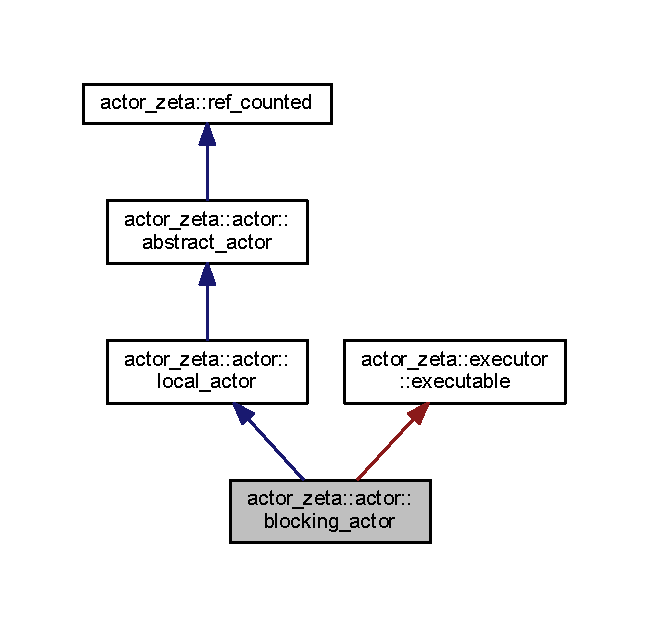
\includegraphics[width=311pt]{classactor__zeta_1_1actor_1_1blocking__actor__inherit__graph}
\end{center}
\end{figure}


Collaboration diagram for actor\+\_\+zeta\+:\+:actor\+:\+:blocking\+\_\+actor\+:\nopagebreak
\begin{figure}[H]
\begin{center}
\leavevmode
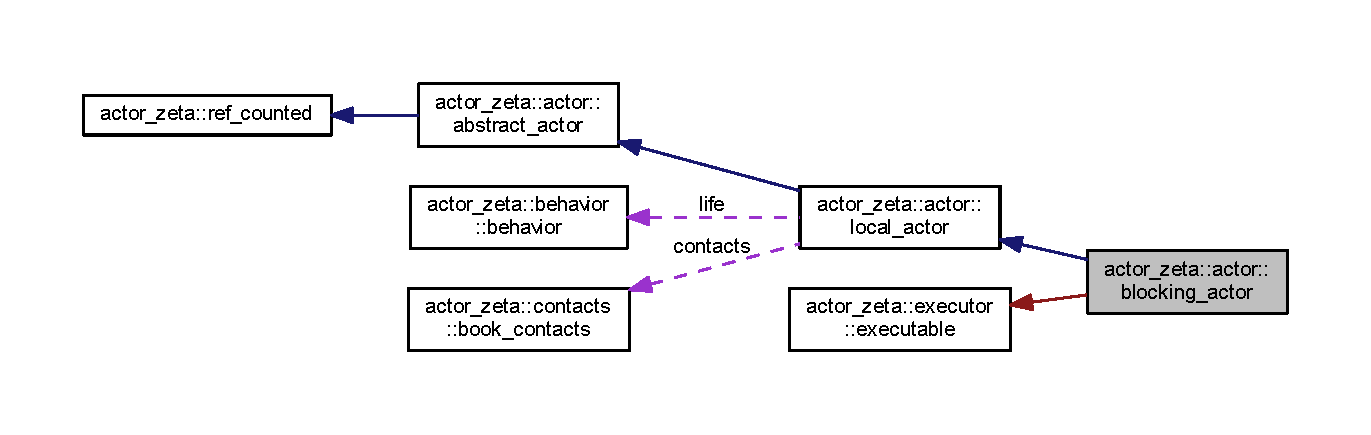
\includegraphics[width=350pt]{classactor__zeta_1_1actor_1_1blocking__actor__coll__graph}
\end{center}
\end{figure}
\subsection*{Public Member Functions}
\begin{DoxyCompactItemize}
\item 
\hyperlink{classactor__zeta_1_1actor_1_1blocking__actor_ab62ea915e7f8597c5f926374a7ab9980}{blocking\+\_\+actor} (\hyperlink{classactor__zeta_1_1environment_1_1environment}{environment\+::environment} $\ast$, const std\+::string \&)
\item 
virtual void \hyperlink{classactor__zeta_1_1actor_1_1blocking__actor_addc9a92e1d9be856cc1842a5c43867f5}{act} ()
\item 
\hyperlink{structactor__zeta_1_1executor_1_1executable_aef06c63be7b22b021ade4b83ed4f3cc4}{executor\+::executable\+::executable\+\_\+result} \hyperlink{classactor__zeta_1_1actor_1_1blocking__actor_af92ae4139344b002f8014433f64f8e56}{run} (\hyperlink{structactor__zeta_1_1executor_1_1execution__device}{executor\+::execution\+\_\+device} $\ast$, size\+\_\+t) override final
\item 
void \hyperlink{classactor__zeta_1_1actor_1_1blocking__actor_a7988829bb7d264b3f226f8c5d4156cb1}{launch} (\hyperlink{structactor__zeta_1_1executor_1_1execution__device}{executor\+::execution\+\_\+device} $\ast$, bool) override final
\item 
virtual \hyperlink{classactor__zeta_1_1actor_1_1blocking__actor_ad78b5512e561def8197df4f5cfbba540}{$\sim$blocking\+\_\+actor} ()
\end{DoxyCompactItemize}
\subsection*{Additional Inherited Members}


\subsection{Detailed Description}
Represents actor type with blocking mode. 

\subsection{Constructor \& Destructor Documentation}
\mbox{\Hypertarget{classactor__zeta_1_1actor_1_1blocking__actor_ab62ea915e7f8597c5f926374a7ab9980}\label{classactor__zeta_1_1actor_1_1blocking__actor_ab62ea915e7f8597c5f926374a7ab9980}} 
\index{actor\+\_\+zeta\+::actor\+::blocking\+\_\+actor@{actor\+\_\+zeta\+::actor\+::blocking\+\_\+actor}!blocking\+\_\+actor@{blocking\+\_\+actor}}
\index{blocking\+\_\+actor@{blocking\+\_\+actor}!actor\+\_\+zeta\+::actor\+::blocking\+\_\+actor@{actor\+\_\+zeta\+::actor\+::blocking\+\_\+actor}}
\subsubsection{\texorpdfstring{blocking\+\_\+actor()}{blocking\_actor()}}
{\footnotesize\ttfamily actor\+\_\+zeta\+::actor\+::blocking\+\_\+actor\+::blocking\+\_\+actor (\begin{DoxyParamCaption}\item[{\hyperlink{classactor__zeta_1_1environment_1_1environment}{environment\+::environment} $\ast$}]{env,  }\item[{const std\+::string \&}]{type }\end{DoxyParamCaption})}

\mbox{\Hypertarget{classactor__zeta_1_1actor_1_1blocking__actor_ad78b5512e561def8197df4f5cfbba540}\label{classactor__zeta_1_1actor_1_1blocking__actor_ad78b5512e561def8197df4f5cfbba540}} 
\index{actor\+\_\+zeta\+::actor\+::blocking\+\_\+actor@{actor\+\_\+zeta\+::actor\+::blocking\+\_\+actor}!````~blocking\+\_\+actor@{$\sim$blocking\+\_\+actor}}
\index{````~blocking\+\_\+actor@{$\sim$blocking\+\_\+actor}!actor\+\_\+zeta\+::actor\+::blocking\+\_\+actor@{actor\+\_\+zeta\+::actor\+::blocking\+\_\+actor}}
\subsubsection{\texorpdfstring{$\sim$blocking\+\_\+actor()}{~blocking\_actor()}}
{\footnotesize\ttfamily virtual actor\+\_\+zeta\+::actor\+::blocking\+\_\+actor\+::$\sim$blocking\+\_\+actor (\begin{DoxyParamCaption}{ }\end{DoxyParamCaption})\hspace{0.3cm}{\ttfamily [inline]}, {\ttfamily [virtual]}}



\subsection{Member Function Documentation}
\mbox{\Hypertarget{classactor__zeta_1_1actor_1_1blocking__actor_addc9a92e1d9be856cc1842a5c43867f5}\label{classactor__zeta_1_1actor_1_1blocking__actor_addc9a92e1d9be856cc1842a5c43867f5}} 
\index{actor\+\_\+zeta\+::actor\+::blocking\+\_\+actor@{actor\+\_\+zeta\+::actor\+::blocking\+\_\+actor}!act@{act}}
\index{act@{act}!actor\+\_\+zeta\+::actor\+::blocking\+\_\+actor@{actor\+\_\+zeta\+::actor\+::blocking\+\_\+actor}}
\subsubsection{\texorpdfstring{act()}{act()}}
{\footnotesize\ttfamily void actor\+\_\+zeta\+::actor\+::blocking\+\_\+actor\+::act (\begin{DoxyParamCaption}{ }\end{DoxyParamCaption})\hspace{0.3cm}{\ttfamily [virtual]}}

\mbox{\Hypertarget{classactor__zeta_1_1actor_1_1blocking__actor_a7988829bb7d264b3f226f8c5d4156cb1}\label{classactor__zeta_1_1actor_1_1blocking__actor_a7988829bb7d264b3f226f8c5d4156cb1}} 
\index{actor\+\_\+zeta\+::actor\+::blocking\+\_\+actor@{actor\+\_\+zeta\+::actor\+::blocking\+\_\+actor}!launch@{launch}}
\index{launch@{launch}!actor\+\_\+zeta\+::actor\+::blocking\+\_\+actor@{actor\+\_\+zeta\+::actor\+::blocking\+\_\+actor}}
\subsubsection{\texorpdfstring{launch()}{launch()}}
{\footnotesize\ttfamily void actor\+\_\+zeta\+::actor\+::blocking\+\_\+actor\+::launch (\begin{DoxyParamCaption}\item[{\hyperlink{structactor__zeta_1_1executor_1_1execution__device}{executor\+::execution\+\_\+device} $\ast$}]{e,  }\item[{bool}]{hide }\end{DoxyParamCaption})\hspace{0.3cm}{\ttfamily [final]}, {\ttfamily [override]}, {\ttfamily [virtual]}}



Implements \hyperlink{classactor__zeta_1_1actor_1_1local__actor_acfba412b813aee3250c589bee232f3cd}{actor\+\_\+zeta\+::actor\+::local\+\_\+actor}.

\mbox{\Hypertarget{classactor__zeta_1_1actor_1_1blocking__actor_af92ae4139344b002f8014433f64f8e56}\label{classactor__zeta_1_1actor_1_1blocking__actor_af92ae4139344b002f8014433f64f8e56}} 
\index{actor\+\_\+zeta\+::actor\+::blocking\+\_\+actor@{actor\+\_\+zeta\+::actor\+::blocking\+\_\+actor}!run@{run}}
\index{run@{run}!actor\+\_\+zeta\+::actor\+::blocking\+\_\+actor@{actor\+\_\+zeta\+::actor\+::blocking\+\_\+actor}}
\subsubsection{\texorpdfstring{run()}{run()}}
{\footnotesize\ttfamily \hyperlink{structactor__zeta_1_1executor_1_1executable_aef06c63be7b22b021ade4b83ed4f3cc4}{executor\+::executable\+::executable\+\_\+result} actor\+\_\+zeta\+::actor\+::blocking\+\_\+actor\+::run (\begin{DoxyParamCaption}\item[{\hyperlink{structactor__zeta_1_1executor_1_1execution__device}{executor\+::execution\+\_\+device} $\ast$}]{e,  }\item[{size\+\_\+t}]{max\+\_\+throughput }\end{DoxyParamCaption})\hspace{0.3cm}{\ttfamily [final]}, {\ttfamily [override]}, {\ttfamily [virtual]}}



Implements \hyperlink{structactor__zeta_1_1executor_1_1executable_a61d6cbce8b124e1e5ef80f8befea2a89}{actor\+\_\+zeta\+::executor\+::executable}.



The documentation for this class was generated from the following files\+:\begin{DoxyCompactItemize}
\item 
\hyperlink{blocking__actor_8hpp}{blocking\+\_\+actor.\+hpp}\item 
\hyperlink{blocking__actor_8cpp}{blocking\+\_\+actor.\+cpp}\end{DoxyCompactItemize}

\hypertarget{classactor__zeta_1_1messaging_1_1blocking__mail__queue}{}\section{actor\+\_\+zeta\+:\+:messaging\+:\+:blocking\+\_\+mail\+\_\+queue$<$ T $>$ Class Template Reference}
\label{classactor__zeta_1_1messaging_1_1blocking__mail__queue}\index{actor\+\_\+zeta\+::messaging\+::blocking\+\_\+mail\+\_\+queue$<$ T $>$@{actor\+\_\+zeta\+::messaging\+::blocking\+\_\+mail\+\_\+queue$<$ T $>$}}


A mailbox class for message queue.  




{\ttfamily \#include $<$blocking\+\_\+mail\+\_\+queue.\+hpp$>$}

\subsection*{Public Types}
\begin{DoxyCompactItemize}
\item 
using \hyperlink{classactor__zeta_1_1messaging_1_1blocking__mail__queue_a64432628c6a91d330431fc3299021045}{pointer} = T $\ast$
\item 
using \hyperlink{classactor__zeta_1_1messaging_1_1blocking__mail__queue_a2615c2611ffdb978624dd2eccc75fe57}{const\+\_\+pointer} = const T $\ast$
\item 
using \hyperlink{classactor__zeta_1_1messaging_1_1blocking__mail__queue_a838522d611616b1bd7c46da5fe6895fb}{reference} = T \&
\item 
using \hyperlink{classactor__zeta_1_1messaging_1_1blocking__mail__queue_a6a883fe6a6e606317f85156f957f84fd}{const\+\_\+reference} = const T \&
\item 
using \hyperlink{classactor__zeta_1_1messaging_1_1blocking__mail__queue_a20156eef06b0a688ceeb663097a90862}{cache\+\_\+type} = std\+::list$<$ \hyperlink{classactor__zeta_1_1messaging_1_1blocking__mail__queue_a64432628c6a91d330431fc3299021045}{pointer} $>$
\item 
using \hyperlink{classactor__zeta_1_1messaging_1_1blocking__mail__queue_a3d270721dd7c3e166e39578cc6b761ce}{queue\+\_\+base\+\_\+type} = std\+::list$<$ \hyperlink{classactor__zeta_1_1messaging_1_1blocking__mail__queue_a64432628c6a91d330431fc3299021045}{pointer} $>$
\item 
using \hyperlink{classactor__zeta_1_1messaging_1_1blocking__mail__queue_a61d0417725665aba520dc0a51f1ec37a}{unique\+\_\+lock} = std\+::unique\+\_\+lock$<$ std\+::mutex $>$
\item 
using \hyperlink{classactor__zeta_1_1messaging_1_1blocking__mail__queue_aa98535adfab3ed0daf9f615f6f8edaaa}{lock\+\_\+guard} = std\+::lock\+\_\+guard$<$ std\+::mutex $>$
\end{DoxyCompactItemize}
\subsection*{Public Member Functions}
\begin{DoxyCompactItemize}
\item 
\hyperlink{classactor__zeta_1_1messaging_1_1blocking__mail__queue_a27b186a6995c984fda250ffaa8cdf207}{blocking\+\_\+mail\+\_\+queue} (const \hyperlink{classactor__zeta_1_1messaging_1_1blocking__mail__queue}{blocking\+\_\+mail\+\_\+queue} \&)=delete
\item 
\hyperlink{classactor__zeta_1_1messaging_1_1blocking__mail__queue}{blocking\+\_\+mail\+\_\+queue} \& \hyperlink{classactor__zeta_1_1messaging_1_1blocking__mail__queue_a595342b1b167fd4a889b6d3f2b533d7e}{operator=} (const \hyperlink{classactor__zeta_1_1messaging_1_1blocking__mail__queue}{blocking\+\_\+mail\+\_\+queue} \&)=delete
\item 
\hyperlink{classactor__zeta_1_1messaging_1_1blocking__mail__queue_a22fa153dcd1965874060e33bc88d61c0}{blocking\+\_\+mail\+\_\+queue} (\hyperlink{classactor__zeta_1_1messaging_1_1blocking__mail__queue}{blocking\+\_\+mail\+\_\+queue} \&\&)=default
\item 
\hyperlink{classactor__zeta_1_1messaging_1_1blocking__mail__queue}{blocking\+\_\+mail\+\_\+queue} \& \hyperlink{classactor__zeta_1_1messaging_1_1blocking__mail__queue_ae5041536a45ba1a1fa68a1ac91c407d5}{operator=} (\hyperlink{classactor__zeta_1_1messaging_1_1blocking__mail__queue}{blocking\+\_\+mail\+\_\+queue} \&\&)=default
\item 
\hyperlink{classactor__zeta_1_1messaging_1_1blocking__mail__queue_a0f37b3d45de05f79501f46bcb93fc92f}{blocking\+\_\+mail\+\_\+queue} ()=default
\item 
\hyperlink{classactor__zeta_1_1messaging_1_1blocking__mail__queue_a60c3eee1e67c1fd16b0898933d352cb3}{$\sim$blocking\+\_\+mail\+\_\+queue} ()=default
\item 
\hyperlink{namespaceactor__zeta_1_1messaging_ac2c5f2f473c5a97d779ec63a78d498a1}{enqueue\+\_\+result} \hyperlink{classactor__zeta_1_1messaging_1_1blocking__mail__queue_a738f8b8948ace649ab23b5fb312bf3da}{put} (\hyperlink{classactor__zeta_1_1messaging_1_1blocking__mail__queue_a64432628c6a91d330431fc3299021045}{pointer} m)
\item 
void \hyperlink{classactor__zeta_1_1messaging_1_1blocking__mail__queue_a26fa1043b83e6956362282989cb18f3d}{sync} ()
\item 
\hyperlink{classactor__zeta_1_1messaging_1_1blocking__mail__queue_a64432628c6a91d330431fc3299021045}{pointer} \hyperlink{classactor__zeta_1_1messaging_1_1blocking__mail__queue_ab5d259cfddb68ab54eb7402c61e980b8}{get} ()
\item 
\hyperlink{classactor__zeta_1_1messaging_1_1blocking__mail__queue_a20156eef06b0a688ceeb663097a90862}{cache\+\_\+type} \& \hyperlink{classactor__zeta_1_1messaging_1_1blocking__mail__queue_a0840f187c44e717bb1078cdd38f2aaf7}{low\+\_\+priority\+\_\+cache} ()
\item 
\hyperlink{classactor__zeta_1_1messaging_1_1blocking__mail__queue_a20156eef06b0a688ceeb663097a90862}{cache\+\_\+type} \& \hyperlink{classactor__zeta_1_1messaging_1_1blocking__mail__queue_abd039cc803849fd87da17a18171a0440}{normal\+\_\+priority\+\_\+cache} ()
\item 
\hyperlink{classactor__zeta_1_1messaging_1_1blocking__mail__queue_a20156eef06b0a688ceeb663097a90862}{cache\+\_\+type} \& \hyperlink{classactor__zeta_1_1messaging_1_1blocking__mail__queue_ad68ddf70deb082f37a154186c75f82bd}{high\+\_\+priority\+\_\+cache} ()
\end{DoxyCompactItemize}


\subsection{Detailed Description}
\subsubsection*{template$<$typename T$>$\newline
class actor\+\_\+zeta\+::messaging\+::blocking\+\_\+mail\+\_\+queue$<$ T $>$}

A mailbox class for message queue. 


\begin{DoxyTemplParams}{Template Parameters}
{\em T} & \\
\hline
\end{DoxyTemplParams}


\subsection{Member Typedef Documentation}
\mbox{\Hypertarget{classactor__zeta_1_1messaging_1_1blocking__mail__queue_a20156eef06b0a688ceeb663097a90862}\label{classactor__zeta_1_1messaging_1_1blocking__mail__queue_a20156eef06b0a688ceeb663097a90862}} 
\index{actor\+\_\+zeta\+::messaging\+::blocking\+\_\+mail\+\_\+queue@{actor\+\_\+zeta\+::messaging\+::blocking\+\_\+mail\+\_\+queue}!cache\+\_\+type@{cache\+\_\+type}}
\index{cache\+\_\+type@{cache\+\_\+type}!actor\+\_\+zeta\+::messaging\+::blocking\+\_\+mail\+\_\+queue@{actor\+\_\+zeta\+::messaging\+::blocking\+\_\+mail\+\_\+queue}}
\subsubsection{\texorpdfstring{cache\+\_\+type}{cache\_type}}
{\footnotesize\ttfamily template$<$typename T$>$ \\
using \hyperlink{classactor__zeta_1_1messaging_1_1blocking__mail__queue}{actor\+\_\+zeta\+::messaging\+::blocking\+\_\+mail\+\_\+queue}$<$ T $>$\+::\hyperlink{classactor__zeta_1_1messaging_1_1blocking__mail__queue_a20156eef06b0a688ceeb663097a90862}{cache\+\_\+type} =  std\+::list$<$\hyperlink{classactor__zeta_1_1messaging_1_1blocking__mail__queue_a64432628c6a91d330431fc3299021045}{pointer}$>$}

\mbox{\Hypertarget{classactor__zeta_1_1messaging_1_1blocking__mail__queue_a2615c2611ffdb978624dd2eccc75fe57}\label{classactor__zeta_1_1messaging_1_1blocking__mail__queue_a2615c2611ffdb978624dd2eccc75fe57}} 
\index{actor\+\_\+zeta\+::messaging\+::blocking\+\_\+mail\+\_\+queue@{actor\+\_\+zeta\+::messaging\+::blocking\+\_\+mail\+\_\+queue}!const\+\_\+pointer@{const\+\_\+pointer}}
\index{const\+\_\+pointer@{const\+\_\+pointer}!actor\+\_\+zeta\+::messaging\+::blocking\+\_\+mail\+\_\+queue@{actor\+\_\+zeta\+::messaging\+::blocking\+\_\+mail\+\_\+queue}}
\subsubsection{\texorpdfstring{const\+\_\+pointer}{const\_pointer}}
{\footnotesize\ttfamily template$<$typename T$>$ \\
using \hyperlink{classactor__zeta_1_1messaging_1_1blocking__mail__queue}{actor\+\_\+zeta\+::messaging\+::blocking\+\_\+mail\+\_\+queue}$<$ T $>$\+::\hyperlink{classactor__zeta_1_1messaging_1_1blocking__mail__queue_a2615c2611ffdb978624dd2eccc75fe57}{const\+\_\+pointer} =  const T $\ast$}

\mbox{\Hypertarget{classactor__zeta_1_1messaging_1_1blocking__mail__queue_a6a883fe6a6e606317f85156f957f84fd}\label{classactor__zeta_1_1messaging_1_1blocking__mail__queue_a6a883fe6a6e606317f85156f957f84fd}} 
\index{actor\+\_\+zeta\+::messaging\+::blocking\+\_\+mail\+\_\+queue@{actor\+\_\+zeta\+::messaging\+::blocking\+\_\+mail\+\_\+queue}!const\+\_\+reference@{const\+\_\+reference}}
\index{const\+\_\+reference@{const\+\_\+reference}!actor\+\_\+zeta\+::messaging\+::blocking\+\_\+mail\+\_\+queue@{actor\+\_\+zeta\+::messaging\+::blocking\+\_\+mail\+\_\+queue}}
\subsubsection{\texorpdfstring{const\+\_\+reference}{const\_reference}}
{\footnotesize\ttfamily template$<$typename T$>$ \\
using \hyperlink{classactor__zeta_1_1messaging_1_1blocking__mail__queue}{actor\+\_\+zeta\+::messaging\+::blocking\+\_\+mail\+\_\+queue}$<$ T $>$\+::\hyperlink{classactor__zeta_1_1messaging_1_1blocking__mail__queue_a6a883fe6a6e606317f85156f957f84fd}{const\+\_\+reference} =  const T \&}

\mbox{\Hypertarget{classactor__zeta_1_1messaging_1_1blocking__mail__queue_aa98535adfab3ed0daf9f615f6f8edaaa}\label{classactor__zeta_1_1messaging_1_1blocking__mail__queue_aa98535adfab3ed0daf9f615f6f8edaaa}} 
\index{actor\+\_\+zeta\+::messaging\+::blocking\+\_\+mail\+\_\+queue@{actor\+\_\+zeta\+::messaging\+::blocking\+\_\+mail\+\_\+queue}!lock\+\_\+guard@{lock\+\_\+guard}}
\index{lock\+\_\+guard@{lock\+\_\+guard}!actor\+\_\+zeta\+::messaging\+::blocking\+\_\+mail\+\_\+queue@{actor\+\_\+zeta\+::messaging\+::blocking\+\_\+mail\+\_\+queue}}
\subsubsection{\texorpdfstring{lock\+\_\+guard}{lock\_guard}}
{\footnotesize\ttfamily template$<$typename T$>$ \\
using \hyperlink{classactor__zeta_1_1messaging_1_1blocking__mail__queue}{actor\+\_\+zeta\+::messaging\+::blocking\+\_\+mail\+\_\+queue}$<$ T $>$\+::\hyperlink{classactor__zeta_1_1messaging_1_1blocking__mail__queue_aa98535adfab3ed0daf9f615f6f8edaaa}{lock\+\_\+guard} =  std\+::lock\+\_\+guard$<$std\+::mutex$>$}

\mbox{\Hypertarget{classactor__zeta_1_1messaging_1_1blocking__mail__queue_a64432628c6a91d330431fc3299021045}\label{classactor__zeta_1_1messaging_1_1blocking__mail__queue_a64432628c6a91d330431fc3299021045}} 
\index{actor\+\_\+zeta\+::messaging\+::blocking\+\_\+mail\+\_\+queue@{actor\+\_\+zeta\+::messaging\+::blocking\+\_\+mail\+\_\+queue}!pointer@{pointer}}
\index{pointer@{pointer}!actor\+\_\+zeta\+::messaging\+::blocking\+\_\+mail\+\_\+queue@{actor\+\_\+zeta\+::messaging\+::blocking\+\_\+mail\+\_\+queue}}
\subsubsection{\texorpdfstring{pointer}{pointer}}
{\footnotesize\ttfamily template$<$typename T$>$ \\
using \hyperlink{classactor__zeta_1_1messaging_1_1blocking__mail__queue}{actor\+\_\+zeta\+::messaging\+::blocking\+\_\+mail\+\_\+queue}$<$ T $>$\+::\hyperlink{classactor__zeta_1_1messaging_1_1blocking__mail__queue_a64432628c6a91d330431fc3299021045}{pointer} =  T $\ast$}

\mbox{\Hypertarget{classactor__zeta_1_1messaging_1_1blocking__mail__queue_a3d270721dd7c3e166e39578cc6b761ce}\label{classactor__zeta_1_1messaging_1_1blocking__mail__queue_a3d270721dd7c3e166e39578cc6b761ce}} 
\index{actor\+\_\+zeta\+::messaging\+::blocking\+\_\+mail\+\_\+queue@{actor\+\_\+zeta\+::messaging\+::blocking\+\_\+mail\+\_\+queue}!queue\+\_\+base\+\_\+type@{queue\+\_\+base\+\_\+type}}
\index{queue\+\_\+base\+\_\+type@{queue\+\_\+base\+\_\+type}!actor\+\_\+zeta\+::messaging\+::blocking\+\_\+mail\+\_\+queue@{actor\+\_\+zeta\+::messaging\+::blocking\+\_\+mail\+\_\+queue}}
\subsubsection{\texorpdfstring{queue\+\_\+base\+\_\+type}{queue\_base\_type}}
{\footnotesize\ttfamily template$<$typename T$>$ \\
using \hyperlink{classactor__zeta_1_1messaging_1_1blocking__mail__queue}{actor\+\_\+zeta\+::messaging\+::blocking\+\_\+mail\+\_\+queue}$<$ T $>$\+::\hyperlink{classactor__zeta_1_1messaging_1_1blocking__mail__queue_a3d270721dd7c3e166e39578cc6b761ce}{queue\+\_\+base\+\_\+type} =  std\+::list$<$\hyperlink{classactor__zeta_1_1messaging_1_1blocking__mail__queue_a64432628c6a91d330431fc3299021045}{pointer}$>$}

\mbox{\Hypertarget{classactor__zeta_1_1messaging_1_1blocking__mail__queue_a838522d611616b1bd7c46da5fe6895fb}\label{classactor__zeta_1_1messaging_1_1blocking__mail__queue_a838522d611616b1bd7c46da5fe6895fb}} 
\index{actor\+\_\+zeta\+::messaging\+::blocking\+\_\+mail\+\_\+queue@{actor\+\_\+zeta\+::messaging\+::blocking\+\_\+mail\+\_\+queue}!reference@{reference}}
\index{reference@{reference}!actor\+\_\+zeta\+::messaging\+::blocking\+\_\+mail\+\_\+queue@{actor\+\_\+zeta\+::messaging\+::blocking\+\_\+mail\+\_\+queue}}
\subsubsection{\texorpdfstring{reference}{reference}}
{\footnotesize\ttfamily template$<$typename T$>$ \\
using \hyperlink{classactor__zeta_1_1messaging_1_1blocking__mail__queue}{actor\+\_\+zeta\+::messaging\+::blocking\+\_\+mail\+\_\+queue}$<$ T $>$\+::\hyperlink{classactor__zeta_1_1messaging_1_1blocking__mail__queue_a838522d611616b1bd7c46da5fe6895fb}{reference} =  T \&}

\mbox{\Hypertarget{classactor__zeta_1_1messaging_1_1blocking__mail__queue_a61d0417725665aba520dc0a51f1ec37a}\label{classactor__zeta_1_1messaging_1_1blocking__mail__queue_a61d0417725665aba520dc0a51f1ec37a}} 
\index{actor\+\_\+zeta\+::messaging\+::blocking\+\_\+mail\+\_\+queue@{actor\+\_\+zeta\+::messaging\+::blocking\+\_\+mail\+\_\+queue}!unique\+\_\+lock@{unique\+\_\+lock}}
\index{unique\+\_\+lock@{unique\+\_\+lock}!actor\+\_\+zeta\+::messaging\+::blocking\+\_\+mail\+\_\+queue@{actor\+\_\+zeta\+::messaging\+::blocking\+\_\+mail\+\_\+queue}}
\subsubsection{\texorpdfstring{unique\+\_\+lock}{unique\_lock}}
{\footnotesize\ttfamily template$<$typename T$>$ \\
using \hyperlink{classactor__zeta_1_1messaging_1_1blocking__mail__queue}{actor\+\_\+zeta\+::messaging\+::blocking\+\_\+mail\+\_\+queue}$<$ T $>$\+::\hyperlink{classactor__zeta_1_1messaging_1_1blocking__mail__queue_a61d0417725665aba520dc0a51f1ec37a}{unique\+\_\+lock} =  std\+::unique\+\_\+lock$<$std\+::mutex$>$}



\subsection{Constructor \& Destructor Documentation}
\mbox{\Hypertarget{classactor__zeta_1_1messaging_1_1blocking__mail__queue_a27b186a6995c984fda250ffaa8cdf207}\label{classactor__zeta_1_1messaging_1_1blocking__mail__queue_a27b186a6995c984fda250ffaa8cdf207}} 
\index{actor\+\_\+zeta\+::messaging\+::blocking\+\_\+mail\+\_\+queue@{actor\+\_\+zeta\+::messaging\+::blocking\+\_\+mail\+\_\+queue}!blocking\+\_\+mail\+\_\+queue@{blocking\+\_\+mail\+\_\+queue}}
\index{blocking\+\_\+mail\+\_\+queue@{blocking\+\_\+mail\+\_\+queue}!actor\+\_\+zeta\+::messaging\+::blocking\+\_\+mail\+\_\+queue@{actor\+\_\+zeta\+::messaging\+::blocking\+\_\+mail\+\_\+queue}}
\subsubsection{\texorpdfstring{blocking\+\_\+mail\+\_\+queue()}{blocking\_mail\_queue()}\hspace{0.1cm}{\footnotesize\ttfamily [1/3]}}
{\footnotesize\ttfamily template$<$typename T$>$ \\
\hyperlink{classactor__zeta_1_1messaging_1_1blocking__mail__queue}{actor\+\_\+zeta\+::messaging\+::blocking\+\_\+mail\+\_\+queue}$<$ T $>$\+::\hyperlink{classactor__zeta_1_1messaging_1_1blocking__mail__queue}{blocking\+\_\+mail\+\_\+queue} (\begin{DoxyParamCaption}\item[{const \hyperlink{classactor__zeta_1_1messaging_1_1blocking__mail__queue}{blocking\+\_\+mail\+\_\+queue}$<$ T $>$ \&}]{ }\end{DoxyParamCaption})\hspace{0.3cm}{\ttfamily [delete]}}

\mbox{\Hypertarget{classactor__zeta_1_1messaging_1_1blocking__mail__queue_a22fa153dcd1965874060e33bc88d61c0}\label{classactor__zeta_1_1messaging_1_1blocking__mail__queue_a22fa153dcd1965874060e33bc88d61c0}} 
\index{actor\+\_\+zeta\+::messaging\+::blocking\+\_\+mail\+\_\+queue@{actor\+\_\+zeta\+::messaging\+::blocking\+\_\+mail\+\_\+queue}!blocking\+\_\+mail\+\_\+queue@{blocking\+\_\+mail\+\_\+queue}}
\index{blocking\+\_\+mail\+\_\+queue@{blocking\+\_\+mail\+\_\+queue}!actor\+\_\+zeta\+::messaging\+::blocking\+\_\+mail\+\_\+queue@{actor\+\_\+zeta\+::messaging\+::blocking\+\_\+mail\+\_\+queue}}
\subsubsection{\texorpdfstring{blocking\+\_\+mail\+\_\+queue()}{blocking\_mail\_queue()}\hspace{0.1cm}{\footnotesize\ttfamily [2/3]}}
{\footnotesize\ttfamily template$<$typename T$>$ \\
\hyperlink{classactor__zeta_1_1messaging_1_1blocking__mail__queue}{actor\+\_\+zeta\+::messaging\+::blocking\+\_\+mail\+\_\+queue}$<$ T $>$\+::\hyperlink{classactor__zeta_1_1messaging_1_1blocking__mail__queue}{blocking\+\_\+mail\+\_\+queue} (\begin{DoxyParamCaption}\item[{\hyperlink{classactor__zeta_1_1messaging_1_1blocking__mail__queue}{blocking\+\_\+mail\+\_\+queue}$<$ T $>$ \&\&}]{ }\end{DoxyParamCaption})\hspace{0.3cm}{\ttfamily [default]}}

\mbox{\Hypertarget{classactor__zeta_1_1messaging_1_1blocking__mail__queue_a0f37b3d45de05f79501f46bcb93fc92f}\label{classactor__zeta_1_1messaging_1_1blocking__mail__queue_a0f37b3d45de05f79501f46bcb93fc92f}} 
\index{actor\+\_\+zeta\+::messaging\+::blocking\+\_\+mail\+\_\+queue@{actor\+\_\+zeta\+::messaging\+::blocking\+\_\+mail\+\_\+queue}!blocking\+\_\+mail\+\_\+queue@{blocking\+\_\+mail\+\_\+queue}}
\index{blocking\+\_\+mail\+\_\+queue@{blocking\+\_\+mail\+\_\+queue}!actor\+\_\+zeta\+::messaging\+::blocking\+\_\+mail\+\_\+queue@{actor\+\_\+zeta\+::messaging\+::blocking\+\_\+mail\+\_\+queue}}
\subsubsection{\texorpdfstring{blocking\+\_\+mail\+\_\+queue()}{blocking\_mail\_queue()}\hspace{0.1cm}{\footnotesize\ttfamily [3/3]}}
{\footnotesize\ttfamily template$<$typename T$>$ \\
\hyperlink{classactor__zeta_1_1messaging_1_1blocking__mail__queue}{actor\+\_\+zeta\+::messaging\+::blocking\+\_\+mail\+\_\+queue}$<$ T $>$\+::\hyperlink{classactor__zeta_1_1messaging_1_1blocking__mail__queue}{blocking\+\_\+mail\+\_\+queue} (\begin{DoxyParamCaption}{ }\end{DoxyParamCaption})\hspace{0.3cm}{\ttfamily [default]}}

\mbox{\Hypertarget{classactor__zeta_1_1messaging_1_1blocking__mail__queue_a60c3eee1e67c1fd16b0898933d352cb3}\label{classactor__zeta_1_1messaging_1_1blocking__mail__queue_a60c3eee1e67c1fd16b0898933d352cb3}} 
\index{actor\+\_\+zeta\+::messaging\+::blocking\+\_\+mail\+\_\+queue@{actor\+\_\+zeta\+::messaging\+::blocking\+\_\+mail\+\_\+queue}!````~blocking\+\_\+mail\+\_\+queue@{$\sim$blocking\+\_\+mail\+\_\+queue}}
\index{````~blocking\+\_\+mail\+\_\+queue@{$\sim$blocking\+\_\+mail\+\_\+queue}!actor\+\_\+zeta\+::messaging\+::blocking\+\_\+mail\+\_\+queue@{actor\+\_\+zeta\+::messaging\+::blocking\+\_\+mail\+\_\+queue}}
\subsubsection{\texorpdfstring{$\sim$blocking\+\_\+mail\+\_\+queue()}{~blocking\_mail\_queue()}}
{\footnotesize\ttfamily template$<$typename T$>$ \\
\hyperlink{classactor__zeta_1_1messaging_1_1blocking__mail__queue}{actor\+\_\+zeta\+::messaging\+::blocking\+\_\+mail\+\_\+queue}$<$ T $>$\+::$\sim$\hyperlink{classactor__zeta_1_1messaging_1_1blocking__mail__queue}{blocking\+\_\+mail\+\_\+queue} (\begin{DoxyParamCaption}{ }\end{DoxyParamCaption})\hspace{0.3cm}{\ttfamily [default]}}



\subsection{Member Function Documentation}
\mbox{\Hypertarget{classactor__zeta_1_1messaging_1_1blocking__mail__queue_ab5d259cfddb68ab54eb7402c61e980b8}\label{classactor__zeta_1_1messaging_1_1blocking__mail__queue_ab5d259cfddb68ab54eb7402c61e980b8}} 
\index{actor\+\_\+zeta\+::messaging\+::blocking\+\_\+mail\+\_\+queue@{actor\+\_\+zeta\+::messaging\+::blocking\+\_\+mail\+\_\+queue}!get@{get}}
\index{get@{get}!actor\+\_\+zeta\+::messaging\+::blocking\+\_\+mail\+\_\+queue@{actor\+\_\+zeta\+::messaging\+::blocking\+\_\+mail\+\_\+queue}}
\subsubsection{\texorpdfstring{get()}{get()}}
{\footnotesize\ttfamily template$<$typename T$>$ \\
\hyperlink{classactor__zeta_1_1messaging_1_1blocking__mail__queue_a64432628c6a91d330431fc3299021045}{pointer} \hyperlink{classactor__zeta_1_1messaging_1_1blocking__mail__queue}{actor\+\_\+zeta\+::messaging\+::blocking\+\_\+mail\+\_\+queue}$<$ T $>$\+::get (\begin{DoxyParamCaption}{ }\end{DoxyParamCaption})\hspace{0.3cm}{\ttfamily [inline]}}

\mbox{\Hypertarget{classactor__zeta_1_1messaging_1_1blocking__mail__queue_ad68ddf70deb082f37a154186c75f82bd}\label{classactor__zeta_1_1messaging_1_1blocking__mail__queue_ad68ddf70deb082f37a154186c75f82bd}} 
\index{actor\+\_\+zeta\+::messaging\+::blocking\+\_\+mail\+\_\+queue@{actor\+\_\+zeta\+::messaging\+::blocking\+\_\+mail\+\_\+queue}!high\+\_\+priority\+\_\+cache@{high\+\_\+priority\+\_\+cache}}
\index{high\+\_\+priority\+\_\+cache@{high\+\_\+priority\+\_\+cache}!actor\+\_\+zeta\+::messaging\+::blocking\+\_\+mail\+\_\+queue@{actor\+\_\+zeta\+::messaging\+::blocking\+\_\+mail\+\_\+queue}}
\subsubsection{\texorpdfstring{high\+\_\+priority\+\_\+cache()}{high\_priority\_cache()}}
{\footnotesize\ttfamily template$<$typename T$>$ \\
\hyperlink{classactor__zeta_1_1messaging_1_1blocking__mail__queue_a20156eef06b0a688ceeb663097a90862}{cache\+\_\+type}\& \hyperlink{classactor__zeta_1_1messaging_1_1blocking__mail__queue}{actor\+\_\+zeta\+::messaging\+::blocking\+\_\+mail\+\_\+queue}$<$ T $>$\+::high\+\_\+priority\+\_\+cache (\begin{DoxyParamCaption}{ }\end{DoxyParamCaption})\hspace{0.3cm}{\ttfamily [inline]}}

\mbox{\Hypertarget{classactor__zeta_1_1messaging_1_1blocking__mail__queue_a0840f187c44e717bb1078cdd38f2aaf7}\label{classactor__zeta_1_1messaging_1_1blocking__mail__queue_a0840f187c44e717bb1078cdd38f2aaf7}} 
\index{actor\+\_\+zeta\+::messaging\+::blocking\+\_\+mail\+\_\+queue@{actor\+\_\+zeta\+::messaging\+::blocking\+\_\+mail\+\_\+queue}!low\+\_\+priority\+\_\+cache@{low\+\_\+priority\+\_\+cache}}
\index{low\+\_\+priority\+\_\+cache@{low\+\_\+priority\+\_\+cache}!actor\+\_\+zeta\+::messaging\+::blocking\+\_\+mail\+\_\+queue@{actor\+\_\+zeta\+::messaging\+::blocking\+\_\+mail\+\_\+queue}}
\subsubsection{\texorpdfstring{low\+\_\+priority\+\_\+cache()}{low\_priority\_cache()}}
{\footnotesize\ttfamily template$<$typename T$>$ \\
\hyperlink{classactor__zeta_1_1messaging_1_1blocking__mail__queue_a20156eef06b0a688ceeb663097a90862}{cache\+\_\+type}\& \hyperlink{classactor__zeta_1_1messaging_1_1blocking__mail__queue}{actor\+\_\+zeta\+::messaging\+::blocking\+\_\+mail\+\_\+queue}$<$ T $>$\+::low\+\_\+priority\+\_\+cache (\begin{DoxyParamCaption}{ }\end{DoxyParamCaption})\hspace{0.3cm}{\ttfamily [inline]}}

\mbox{\Hypertarget{classactor__zeta_1_1messaging_1_1blocking__mail__queue_abd039cc803849fd87da17a18171a0440}\label{classactor__zeta_1_1messaging_1_1blocking__mail__queue_abd039cc803849fd87da17a18171a0440}} 
\index{actor\+\_\+zeta\+::messaging\+::blocking\+\_\+mail\+\_\+queue@{actor\+\_\+zeta\+::messaging\+::blocking\+\_\+mail\+\_\+queue}!normal\+\_\+priority\+\_\+cache@{normal\+\_\+priority\+\_\+cache}}
\index{normal\+\_\+priority\+\_\+cache@{normal\+\_\+priority\+\_\+cache}!actor\+\_\+zeta\+::messaging\+::blocking\+\_\+mail\+\_\+queue@{actor\+\_\+zeta\+::messaging\+::blocking\+\_\+mail\+\_\+queue}}
\subsubsection{\texorpdfstring{normal\+\_\+priority\+\_\+cache()}{normal\_priority\_cache()}}
{\footnotesize\ttfamily template$<$typename T$>$ \\
\hyperlink{classactor__zeta_1_1messaging_1_1blocking__mail__queue_a20156eef06b0a688ceeb663097a90862}{cache\+\_\+type}\& \hyperlink{classactor__zeta_1_1messaging_1_1blocking__mail__queue}{actor\+\_\+zeta\+::messaging\+::blocking\+\_\+mail\+\_\+queue}$<$ T $>$\+::normal\+\_\+priority\+\_\+cache (\begin{DoxyParamCaption}{ }\end{DoxyParamCaption})\hspace{0.3cm}{\ttfamily [inline]}}

\mbox{\Hypertarget{classactor__zeta_1_1messaging_1_1blocking__mail__queue_a595342b1b167fd4a889b6d3f2b533d7e}\label{classactor__zeta_1_1messaging_1_1blocking__mail__queue_a595342b1b167fd4a889b6d3f2b533d7e}} 
\index{actor\+\_\+zeta\+::messaging\+::blocking\+\_\+mail\+\_\+queue@{actor\+\_\+zeta\+::messaging\+::blocking\+\_\+mail\+\_\+queue}!operator=@{operator=}}
\index{operator=@{operator=}!actor\+\_\+zeta\+::messaging\+::blocking\+\_\+mail\+\_\+queue@{actor\+\_\+zeta\+::messaging\+::blocking\+\_\+mail\+\_\+queue}}
\subsubsection{\texorpdfstring{operator=()}{operator=()}\hspace{0.1cm}{\footnotesize\ttfamily [1/2]}}
{\footnotesize\ttfamily template$<$typename T$>$ \\
\hyperlink{classactor__zeta_1_1messaging_1_1blocking__mail__queue}{blocking\+\_\+mail\+\_\+queue}\& \hyperlink{classactor__zeta_1_1messaging_1_1blocking__mail__queue}{actor\+\_\+zeta\+::messaging\+::blocking\+\_\+mail\+\_\+queue}$<$ T $>$\+::operator= (\begin{DoxyParamCaption}\item[{const \hyperlink{classactor__zeta_1_1messaging_1_1blocking__mail__queue}{blocking\+\_\+mail\+\_\+queue}$<$ T $>$ \&}]{ }\end{DoxyParamCaption})\hspace{0.3cm}{\ttfamily [delete]}}

\mbox{\Hypertarget{classactor__zeta_1_1messaging_1_1blocking__mail__queue_ae5041536a45ba1a1fa68a1ac91c407d5}\label{classactor__zeta_1_1messaging_1_1blocking__mail__queue_ae5041536a45ba1a1fa68a1ac91c407d5}} 
\index{actor\+\_\+zeta\+::messaging\+::blocking\+\_\+mail\+\_\+queue@{actor\+\_\+zeta\+::messaging\+::blocking\+\_\+mail\+\_\+queue}!operator=@{operator=}}
\index{operator=@{operator=}!actor\+\_\+zeta\+::messaging\+::blocking\+\_\+mail\+\_\+queue@{actor\+\_\+zeta\+::messaging\+::blocking\+\_\+mail\+\_\+queue}}
\subsubsection{\texorpdfstring{operator=()}{operator=()}\hspace{0.1cm}{\footnotesize\ttfamily [2/2]}}
{\footnotesize\ttfamily template$<$typename T$>$ \\
\hyperlink{classactor__zeta_1_1messaging_1_1blocking__mail__queue}{blocking\+\_\+mail\+\_\+queue}\& \hyperlink{classactor__zeta_1_1messaging_1_1blocking__mail__queue}{actor\+\_\+zeta\+::messaging\+::blocking\+\_\+mail\+\_\+queue}$<$ T $>$\+::operator= (\begin{DoxyParamCaption}\item[{\hyperlink{classactor__zeta_1_1messaging_1_1blocking__mail__queue}{blocking\+\_\+mail\+\_\+queue}$<$ T $>$ \&\&}]{ }\end{DoxyParamCaption})\hspace{0.3cm}{\ttfamily [default]}}

\mbox{\Hypertarget{classactor__zeta_1_1messaging_1_1blocking__mail__queue_a738f8b8948ace649ab23b5fb312bf3da}\label{classactor__zeta_1_1messaging_1_1blocking__mail__queue_a738f8b8948ace649ab23b5fb312bf3da}} 
\index{actor\+\_\+zeta\+::messaging\+::blocking\+\_\+mail\+\_\+queue@{actor\+\_\+zeta\+::messaging\+::blocking\+\_\+mail\+\_\+queue}!put@{put}}
\index{put@{put}!actor\+\_\+zeta\+::messaging\+::blocking\+\_\+mail\+\_\+queue@{actor\+\_\+zeta\+::messaging\+::blocking\+\_\+mail\+\_\+queue}}
\subsubsection{\texorpdfstring{put()}{put()}}
{\footnotesize\ttfamily template$<$typename T$>$ \\
\hyperlink{namespaceactor__zeta_1_1messaging_ac2c5f2f473c5a97d779ec63a78d498a1}{enqueue\+\_\+result} \hyperlink{classactor__zeta_1_1messaging_1_1blocking__mail__queue}{actor\+\_\+zeta\+::messaging\+::blocking\+\_\+mail\+\_\+queue}$<$ T $>$\+::put (\begin{DoxyParamCaption}\item[{\hyperlink{classactor__zeta_1_1messaging_1_1blocking__mail__queue_a64432628c6a91d330431fc3299021045}{pointer}}]{m }\end{DoxyParamCaption})\hspace{0.3cm}{\ttfamily [inline]}}

\mbox{\Hypertarget{classactor__zeta_1_1messaging_1_1blocking__mail__queue_a26fa1043b83e6956362282989cb18f3d}\label{classactor__zeta_1_1messaging_1_1blocking__mail__queue_a26fa1043b83e6956362282989cb18f3d}} 
\index{actor\+\_\+zeta\+::messaging\+::blocking\+\_\+mail\+\_\+queue@{actor\+\_\+zeta\+::messaging\+::blocking\+\_\+mail\+\_\+queue}!sync@{sync}}
\index{sync@{sync}!actor\+\_\+zeta\+::messaging\+::blocking\+\_\+mail\+\_\+queue@{actor\+\_\+zeta\+::messaging\+::blocking\+\_\+mail\+\_\+queue}}
\subsubsection{\texorpdfstring{sync()}{sync()}}
{\footnotesize\ttfamily template$<$typename T$>$ \\
void \hyperlink{classactor__zeta_1_1messaging_1_1blocking__mail__queue}{actor\+\_\+zeta\+::messaging\+::blocking\+\_\+mail\+\_\+queue}$<$ T $>$\+::sync (\begin{DoxyParamCaption}{ }\end{DoxyParamCaption})\hspace{0.3cm}{\ttfamily [inline]}}



The documentation for this class was generated from the following file\+:\begin{DoxyCompactItemize}
\item 
\hyperlink{blocking__mail__queue_8hpp}{blocking\+\_\+mail\+\_\+queue.\+hpp}\end{DoxyCompactItemize}

\hypertarget{classactor__zeta_1_1contacts_1_1book__contacts}{}\section{actor\+\_\+zeta\+:\+:contacts\+:\+:book\+\_\+contacts Class Reference}
\label{classactor__zeta_1_1contacts_1_1book__contacts}\index{actor\+\_\+zeta\+::contacts\+::book\+\_\+contacts@{actor\+\_\+zeta\+::contacts\+::book\+\_\+contacts}}


Navigation map for actor \& groups.  




{\ttfamily \#include $<$book\+\_\+contacts.\+hpp$>$}

\subsection*{Public Member Functions}
\begin{DoxyCompactItemize}
\item 
\hyperlink{classactor__zeta_1_1contacts_1_1book__contacts_a93162fcc68243ec556e677b3af0ffbb5}{book\+\_\+contacts} ()=default
\item 
\hyperlink{classactor__zeta_1_1contacts_1_1book__contacts_a738055d7898dfc774a991bd976a4cf4a}{book\+\_\+contacts} (\hyperlink{classactor__zeta_1_1contacts_1_1book__contacts}{book\+\_\+contacts} \&\&)=default
\item 
\hyperlink{classactor__zeta_1_1contacts_1_1book__contacts}{book\+\_\+contacts} \& \hyperlink{classactor__zeta_1_1contacts_1_1book__contacts_ab61cdef0f457ecdd0c8adde0b8d2e3fc}{operator=} (\hyperlink{classactor__zeta_1_1contacts_1_1book__contacts}{book\+\_\+contacts} \&\&)=default
\item 
void \hyperlink{classactor__zeta_1_1contacts_1_1book__contacts_a8ae49bfac18a50e9f7e4d1ac8abb1b48}{put} (const \hyperlink{classactor__zeta_1_1actor_1_1actor__address}{actor\+::actor\+\_\+address} \&)
\item 
const \hyperlink{classactor__zeta_1_1actor_1_1actor__address}{actor\+::actor\+\_\+address} \& \hyperlink{classactor__zeta_1_1contacts_1_1book__contacts_ae85462f8140edf9d5d9fb02fc74c76f6}{get} (const std\+::string \&)
\item 
void \hyperlink{classactor__zeta_1_1contacts_1_1book__contacts_a6f0ffb15b767f92dd0b0dd909542d42a}{put\+\_\+in\+\_\+group} (const std\+::string \&, const \hyperlink{classactor__zeta_1_1actor_1_1actor__address}{actor\+::actor\+\_\+address} \&)
\item 
const \hyperlink{classactor__zeta_1_1actor_1_1actor__address}{actor\+::actor\+\_\+address} \& \hyperlink{classactor__zeta_1_1contacts_1_1book__contacts_ab5d2dae8ce93346cb2bb8c3eb3b47371}{get\+\_\+group} (const std\+::string \&)
\item 
void \hyperlink{classactor__zeta_1_1contacts_1_1book__contacts_a7d674e3806ae3a1971e206312bc7983f}{all\+\_\+view} ()
\end{DoxyCompactItemize}


\subsection{Detailed Description}
Navigation map for actor \& groups. 

\subsection{Constructor \& Destructor Documentation}
\mbox{\Hypertarget{classactor__zeta_1_1contacts_1_1book__contacts_a93162fcc68243ec556e677b3af0ffbb5}\label{classactor__zeta_1_1contacts_1_1book__contacts_a93162fcc68243ec556e677b3af0ffbb5}} 
\index{actor\+\_\+zeta\+::contacts\+::book\+\_\+contacts@{actor\+\_\+zeta\+::contacts\+::book\+\_\+contacts}!book\+\_\+contacts@{book\+\_\+contacts}}
\index{book\+\_\+contacts@{book\+\_\+contacts}!actor\+\_\+zeta\+::contacts\+::book\+\_\+contacts@{actor\+\_\+zeta\+::contacts\+::book\+\_\+contacts}}
\subsubsection{\texorpdfstring{book\+\_\+contacts()}{book\_contacts()}\hspace{0.1cm}{\footnotesize\ttfamily [1/2]}}
{\footnotesize\ttfamily actor\+\_\+zeta\+::contacts\+::book\+\_\+contacts\+::book\+\_\+contacts (\begin{DoxyParamCaption}{ }\end{DoxyParamCaption})\hspace{0.3cm}{\ttfamily [default]}}

\mbox{\Hypertarget{classactor__zeta_1_1contacts_1_1book__contacts_a738055d7898dfc774a991bd976a4cf4a}\label{classactor__zeta_1_1contacts_1_1book__contacts_a738055d7898dfc774a991bd976a4cf4a}} 
\index{actor\+\_\+zeta\+::contacts\+::book\+\_\+contacts@{actor\+\_\+zeta\+::contacts\+::book\+\_\+contacts}!book\+\_\+contacts@{book\+\_\+contacts}}
\index{book\+\_\+contacts@{book\+\_\+contacts}!actor\+\_\+zeta\+::contacts\+::book\+\_\+contacts@{actor\+\_\+zeta\+::contacts\+::book\+\_\+contacts}}
\subsubsection{\texorpdfstring{book\+\_\+contacts()}{book\_contacts()}\hspace{0.1cm}{\footnotesize\ttfamily [2/2]}}
{\footnotesize\ttfamily actor\+\_\+zeta\+::contacts\+::book\+\_\+contacts\+::book\+\_\+contacts (\begin{DoxyParamCaption}\item[{\hyperlink{classactor__zeta_1_1contacts_1_1book__contacts}{book\+\_\+contacts} \&\&}]{ }\end{DoxyParamCaption})\hspace{0.3cm}{\ttfamily [default]}}



\subsection{Member Function Documentation}
\mbox{\Hypertarget{classactor__zeta_1_1contacts_1_1book__contacts_a7d674e3806ae3a1971e206312bc7983f}\label{classactor__zeta_1_1contacts_1_1book__contacts_a7d674e3806ae3a1971e206312bc7983f}} 
\index{actor\+\_\+zeta\+::contacts\+::book\+\_\+contacts@{actor\+\_\+zeta\+::contacts\+::book\+\_\+contacts}!all\+\_\+view@{all\+\_\+view}}
\index{all\+\_\+view@{all\+\_\+view}!actor\+\_\+zeta\+::contacts\+::book\+\_\+contacts@{actor\+\_\+zeta\+::contacts\+::book\+\_\+contacts}}
\subsubsection{\texorpdfstring{all\+\_\+view()}{all\_view()}}
{\footnotesize\ttfamily void actor\+\_\+zeta\+::contacts\+::book\+\_\+contacts\+::all\+\_\+view (\begin{DoxyParamCaption}{ }\end{DoxyParamCaption})}

\mbox{\Hypertarget{classactor__zeta_1_1contacts_1_1book__contacts_ae85462f8140edf9d5d9fb02fc74c76f6}\label{classactor__zeta_1_1contacts_1_1book__contacts_ae85462f8140edf9d5d9fb02fc74c76f6}} 
\index{actor\+\_\+zeta\+::contacts\+::book\+\_\+contacts@{actor\+\_\+zeta\+::contacts\+::book\+\_\+contacts}!get@{get}}
\index{get@{get}!actor\+\_\+zeta\+::contacts\+::book\+\_\+contacts@{actor\+\_\+zeta\+::contacts\+::book\+\_\+contacts}}
\subsubsection{\texorpdfstring{get()}{get()}}
{\footnotesize\ttfamily const \hyperlink{classactor__zeta_1_1actor_1_1actor__address}{actor\+::actor\+\_\+address} \& actor\+\_\+zeta\+::contacts\+::book\+\_\+contacts\+::get (\begin{DoxyParamCaption}\item[{const std\+::string \&}]{name }\end{DoxyParamCaption})}

\mbox{\Hypertarget{classactor__zeta_1_1contacts_1_1book__contacts_ab5d2dae8ce93346cb2bb8c3eb3b47371}\label{classactor__zeta_1_1contacts_1_1book__contacts_ab5d2dae8ce93346cb2bb8c3eb3b47371}} 
\index{actor\+\_\+zeta\+::contacts\+::book\+\_\+contacts@{actor\+\_\+zeta\+::contacts\+::book\+\_\+contacts}!get\+\_\+group@{get\+\_\+group}}
\index{get\+\_\+group@{get\+\_\+group}!actor\+\_\+zeta\+::contacts\+::book\+\_\+contacts@{actor\+\_\+zeta\+::contacts\+::book\+\_\+contacts}}
\subsubsection{\texorpdfstring{get\+\_\+group()}{get\_group()}}
{\footnotesize\ttfamily const \hyperlink{classactor__zeta_1_1actor_1_1actor__address}{actor\+::actor\+\_\+address} \& actor\+\_\+zeta\+::contacts\+::book\+\_\+contacts\+::get\+\_\+group (\begin{DoxyParamCaption}\item[{const std\+::string \&}]{name }\end{DoxyParamCaption})}

\mbox{\Hypertarget{classactor__zeta_1_1contacts_1_1book__contacts_ab61cdef0f457ecdd0c8adde0b8d2e3fc}\label{classactor__zeta_1_1contacts_1_1book__contacts_ab61cdef0f457ecdd0c8adde0b8d2e3fc}} 
\index{actor\+\_\+zeta\+::contacts\+::book\+\_\+contacts@{actor\+\_\+zeta\+::contacts\+::book\+\_\+contacts}!operator=@{operator=}}
\index{operator=@{operator=}!actor\+\_\+zeta\+::contacts\+::book\+\_\+contacts@{actor\+\_\+zeta\+::contacts\+::book\+\_\+contacts}}
\subsubsection{\texorpdfstring{operator=()}{operator=()}}
{\footnotesize\ttfamily \hyperlink{classactor__zeta_1_1contacts_1_1book__contacts}{book\+\_\+contacts}\& actor\+\_\+zeta\+::contacts\+::book\+\_\+contacts\+::operator= (\begin{DoxyParamCaption}\item[{\hyperlink{classactor__zeta_1_1contacts_1_1book__contacts}{book\+\_\+contacts} \&\&}]{ }\end{DoxyParamCaption})\hspace{0.3cm}{\ttfamily [default]}}

\mbox{\Hypertarget{classactor__zeta_1_1contacts_1_1book__contacts_a8ae49bfac18a50e9f7e4d1ac8abb1b48}\label{classactor__zeta_1_1contacts_1_1book__contacts_a8ae49bfac18a50e9f7e4d1ac8abb1b48}} 
\index{actor\+\_\+zeta\+::contacts\+::book\+\_\+contacts@{actor\+\_\+zeta\+::contacts\+::book\+\_\+contacts}!put@{put}}
\index{put@{put}!actor\+\_\+zeta\+::contacts\+::book\+\_\+contacts@{actor\+\_\+zeta\+::contacts\+::book\+\_\+contacts}}
\subsubsection{\texorpdfstring{put()}{put()}}
{\footnotesize\ttfamily void actor\+\_\+zeta\+::contacts\+::book\+\_\+contacts\+::put (\begin{DoxyParamCaption}\item[{const \hyperlink{classactor__zeta_1_1actor_1_1actor__address}{actor\+::actor\+\_\+address} \&}]{vc }\end{DoxyParamCaption})}

\mbox{\Hypertarget{classactor__zeta_1_1contacts_1_1book__contacts_a6f0ffb15b767f92dd0b0dd909542d42a}\label{classactor__zeta_1_1contacts_1_1book__contacts_a6f0ffb15b767f92dd0b0dd909542d42a}} 
\index{actor\+\_\+zeta\+::contacts\+::book\+\_\+contacts@{actor\+\_\+zeta\+::contacts\+::book\+\_\+contacts}!put\+\_\+in\+\_\+group@{put\+\_\+in\+\_\+group}}
\index{put\+\_\+in\+\_\+group@{put\+\_\+in\+\_\+group}!actor\+\_\+zeta\+::contacts\+::book\+\_\+contacts@{actor\+\_\+zeta\+::contacts\+::book\+\_\+contacts}}
\subsubsection{\texorpdfstring{put\+\_\+in\+\_\+group()}{put\_in\_group()}}
{\footnotesize\ttfamily void actor\+\_\+zeta\+::contacts\+::book\+\_\+contacts\+::put\+\_\+in\+\_\+group (\begin{DoxyParamCaption}\item[{const std\+::string \&}]{name,  }\item[{const \hyperlink{classactor__zeta_1_1actor_1_1actor__address}{actor\+::actor\+\_\+address} \&}]{address }\end{DoxyParamCaption})}



The documentation for this class was generated from the following files\+:\begin{DoxyCompactItemize}
\item 
\hyperlink{book__contacts_8hpp}{book\+\_\+contacts.\+hpp}\item 
\hyperlink{book__contacts_8cpp}{book\+\_\+contacts.\+cpp}\end{DoxyCompactItemize}

\hypertarget{classactor__zeta_1_1network_1_1broker}{}\section{actor\+\_\+zeta\+:\+:network\+:\+:broker Class Reference}
\label{classactor__zeta_1_1network_1_1broker}\index{actor\+\_\+zeta\+::network\+::broker@{actor\+\_\+zeta\+::network\+::broker}}


A broker for messaging.  




{\ttfamily \#include $<$broker.\+hpp$>$}



Inheritance diagram for actor\+\_\+zeta\+:\+:network\+:\+:broker\+:\nopagebreak
\begin{figure}[H]
\begin{center}
\leavevmode
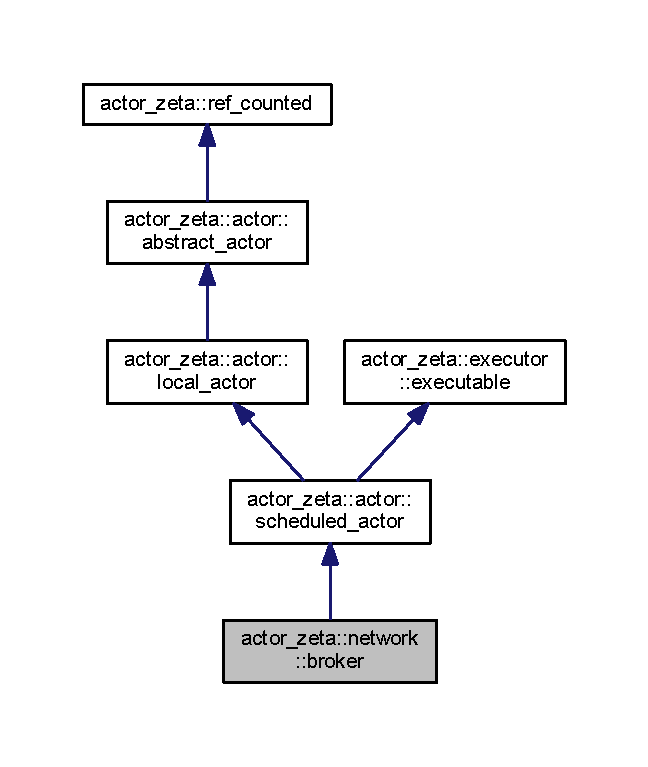
\includegraphics[width=311pt]{classactor__zeta_1_1network_1_1broker__inherit__graph}
\end{center}
\end{figure}


Collaboration diagram for actor\+\_\+zeta\+:\+:network\+:\+:broker\+:\nopagebreak
\begin{figure}[H]
\begin{center}
\leavevmode
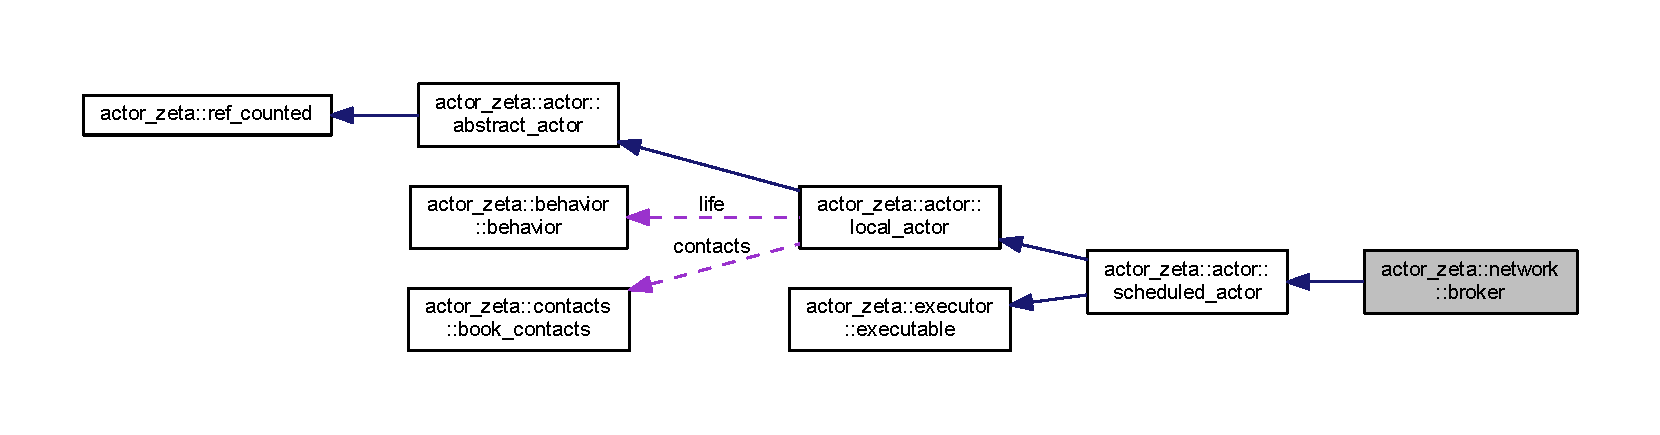
\includegraphics[width=350pt]{classactor__zeta_1_1network_1_1broker__coll__graph}
\end{center}
\end{figure}
\subsection*{Public Member Functions}
\begin{DoxyCompactItemize}
\item 
\hyperlink{classactor__zeta_1_1network_1_1broker_a0e9529d4114718c9b0f34078d1d2ca76}{broker} (\hyperlink{classactor__zeta_1_1environment_1_1environment}{environment\+::environment} $\ast$, const std\+::string \&, \hyperlink{namespaceactor__zeta_1_1network_a504802c43f97832081066e4c7aeb5f24}{shared\+\_\+multiplexer\+\_\+ptr})
\item 
virtual \hyperlink{classactor__zeta_1_1network_1_1broker_aaf24d2099f0c5cbee7d12bc77144f6b3}{$\sim$broker} ()=default
\end{DoxyCompactItemize}
\subsection*{Protected Member Functions}
\begin{DoxyCompactItemize}
\item 
void \hyperlink{classactor__zeta_1_1network_1_1broker_a5e63848370208ff7e670ec08ea7b3cf9}{initialize} () override
\end{DoxyCompactItemize}
\subsection*{Protected Attributes}
\begin{DoxyCompactItemize}
\item 
std\+::shared\+\_\+ptr$<$ \hyperlink{structactor__zeta_1_1network_1_1multiplexer}{multiplexer} $>$ \hyperlink{classactor__zeta_1_1network_1_1broker_aa073d9150fc257a4f39e9571f34d3686}{multiplexer\+\_\+}
\end{DoxyCompactItemize}
\subsection*{Additional Inherited Members}


\subsection{Detailed Description}
A broker for messaging. 

\subsection{Constructor \& Destructor Documentation}
\mbox{\Hypertarget{classactor__zeta_1_1network_1_1broker_a0e9529d4114718c9b0f34078d1d2ca76}\label{classactor__zeta_1_1network_1_1broker_a0e9529d4114718c9b0f34078d1d2ca76}} 
\index{actor\+\_\+zeta\+::network\+::broker@{actor\+\_\+zeta\+::network\+::broker}!broker@{broker}}
\index{broker@{broker}!actor\+\_\+zeta\+::network\+::broker@{actor\+\_\+zeta\+::network\+::broker}}
\subsubsection{\texorpdfstring{broker()}{broker()}}
{\footnotesize\ttfamily actor\+\_\+zeta\+::network\+::broker\+::broker (\begin{DoxyParamCaption}\item[{\hyperlink{classactor__zeta_1_1environment_1_1environment}{environment\+::environment} $\ast$}]{env,  }\item[{const std\+::string \&}]{name,  }\item[{\hyperlink{namespaceactor__zeta_1_1network_a504802c43f97832081066e4c7aeb5f24}{shared\+\_\+multiplexer\+\_\+ptr}}]{m\+\_\+ptr }\end{DoxyParamCaption})}

\mbox{\Hypertarget{classactor__zeta_1_1network_1_1broker_aaf24d2099f0c5cbee7d12bc77144f6b3}\label{classactor__zeta_1_1network_1_1broker_aaf24d2099f0c5cbee7d12bc77144f6b3}} 
\index{actor\+\_\+zeta\+::network\+::broker@{actor\+\_\+zeta\+::network\+::broker}!````~broker@{$\sim$broker}}
\index{````~broker@{$\sim$broker}!actor\+\_\+zeta\+::network\+::broker@{actor\+\_\+zeta\+::network\+::broker}}
\subsubsection{\texorpdfstring{$\sim$broker()}{~broker()}}
{\footnotesize\ttfamily virtual actor\+\_\+zeta\+::network\+::broker\+::$\sim$broker (\begin{DoxyParamCaption}{ }\end{DoxyParamCaption})\hspace{0.3cm}{\ttfamily [virtual]}, {\ttfamily [default]}}



\subsection{Member Function Documentation}
\mbox{\Hypertarget{classactor__zeta_1_1network_1_1broker_a5e63848370208ff7e670ec08ea7b3cf9}\label{classactor__zeta_1_1network_1_1broker_a5e63848370208ff7e670ec08ea7b3cf9}} 
\index{actor\+\_\+zeta\+::network\+::broker@{actor\+\_\+zeta\+::network\+::broker}!initialize@{initialize}}
\index{initialize@{initialize}!actor\+\_\+zeta\+::network\+::broker@{actor\+\_\+zeta\+::network\+::broker}}
\subsubsection{\texorpdfstring{initialize()}{initialize()}}
{\footnotesize\ttfamily void actor\+\_\+zeta\+::network\+::broker\+::initialize (\begin{DoxyParamCaption}{ }\end{DoxyParamCaption})\hspace{0.3cm}{\ttfamily [override]}, {\ttfamily [protected]}, {\ttfamily [virtual]}}



Reimplemented from \hyperlink{classactor__zeta_1_1actor_1_1local__actor_ab540625b83fa06318a2ae41dcca4ca16}{actor\+\_\+zeta\+::actor\+::local\+\_\+actor}.



\subsection{Member Data Documentation}
\mbox{\Hypertarget{classactor__zeta_1_1network_1_1broker_aa073d9150fc257a4f39e9571f34d3686}\label{classactor__zeta_1_1network_1_1broker_aa073d9150fc257a4f39e9571f34d3686}} 
\index{actor\+\_\+zeta\+::network\+::broker@{actor\+\_\+zeta\+::network\+::broker}!multiplexer\+\_\+@{multiplexer\+\_\+}}
\index{multiplexer\+\_\+@{multiplexer\+\_\+}!actor\+\_\+zeta\+::network\+::broker@{actor\+\_\+zeta\+::network\+::broker}}
\subsubsection{\texorpdfstring{multiplexer\+\_\+}{multiplexer\_}}
{\footnotesize\ttfamily std\+::shared\+\_\+ptr$<$\hyperlink{structactor__zeta_1_1network_1_1multiplexer}{multiplexer}$>$ actor\+\_\+zeta\+::network\+::broker\+::multiplexer\+\_\+\hspace{0.3cm}{\ttfamily [protected]}}



The documentation for this class was generated from the following files\+:\begin{DoxyCompactItemize}
\item 
\hyperlink{broker_8hpp}{broker.\+hpp}\item 
\hyperlink{broker_8cpp}{broker.\+cpp}\end{DoxyCompactItemize}

\hypertarget{classactor__zeta_1_1network_1_1connection__identifying}{}\section{actor\+\_\+zeta\+:\+:network\+:\+:connection\+\_\+identifying Class Reference}
\label{classactor__zeta_1_1network_1_1connection__identifying}\index{actor\+\_\+zeta\+::network\+::connection\+\_\+identifying@{actor\+\_\+zeta\+::network\+::connection\+\_\+identifying}}


Implementation of connection functionality.  




{\ttfamily \#include $<$connection\+\_\+identifying.\+hpp$>$}

\subsection*{Public Member Functions}
\begin{DoxyCompactItemize}
\item 
\hyperlink{classactor__zeta_1_1network_1_1connection__identifying_a5d11dde1d79dea149d8d538814673469}{connection\+\_\+identifying} ()=delete
\item 
\hyperlink{classactor__zeta_1_1network_1_1connection__identifying_ae10d0797e40eeb071c5c2d5be418dc41}{connection\+\_\+identifying} (const \hyperlink{classactor__zeta_1_1network_1_1connection__identifying}{connection\+\_\+identifying} \&)=default
\item 
\hyperlink{classactor__zeta_1_1network_1_1connection__identifying}{connection\+\_\+identifying} \& \hyperlink{classactor__zeta_1_1network_1_1connection__identifying_ad7ad59f9a9d998f74662a73265292214}{operator=} (const \hyperlink{classactor__zeta_1_1network_1_1connection__identifying}{connection\+\_\+identifying} \&)=default
\item 
\hyperlink{classactor__zeta_1_1network_1_1connection__identifying_aa95dea5f31545f42ecb43625faea5f11}{connection\+\_\+identifying} (\hyperlink{classactor__zeta_1_1network_1_1connection__identifying}{connection\+\_\+identifying} \&\&)=default
\item 
\hyperlink{classactor__zeta_1_1network_1_1connection__identifying}{connection\+\_\+identifying} \& \hyperlink{classactor__zeta_1_1network_1_1connection__identifying_a9e526832959b3245dcf991ce6dbab047}{operator=} (\hyperlink{classactor__zeta_1_1network_1_1connection__identifying}{connection\+\_\+identifying} \&\&)=default
\item 
\hyperlink{classactor__zeta_1_1network_1_1connection__identifying_a4a1c2a18a3b7bca4a367c3adbf6aa023}{connection\+\_\+identifying} (const \hyperlink{namespaceactor__zeta_1_1network_a4046d5cb8c42554d5787ef4f0d5e3094}{type\+\_\+connect} \&tc, const std\+::string \&ip\+\_\+, const int \&port\+\_\+)
\item 
std\+::string \hyperlink{classactor__zeta_1_1network_1_1connection__identifying_a460e8e57e12ec47497a1a996de5ad82e}{to\+\_\+string} () const
\item 
const std\+::string \& \hyperlink{classactor__zeta_1_1network_1_1connection__identifying_a7acff7d7e92d95168db765ea7816954f}{ip} () const
\item 
const int \& \hyperlink{classactor__zeta_1_1network_1_1connection__identifying_aa5b0146888f91c56a74d96a9853788cf}{port} () const
\item 
bool \hyperlink{classactor__zeta_1_1network_1_1connection__identifying_ab283bc5ac9dcbddaad3140bfabe9f137}{operator==} (const \hyperlink{classactor__zeta_1_1network_1_1connection__identifying}{connection\+\_\+identifying} \&ci) const
\end{DoxyCompactItemize}


\subsection{Detailed Description}
Implementation of connection functionality. 

\subsection{Constructor \& Destructor Documentation}
\mbox{\Hypertarget{classactor__zeta_1_1network_1_1connection__identifying_a5d11dde1d79dea149d8d538814673469}\label{classactor__zeta_1_1network_1_1connection__identifying_a5d11dde1d79dea149d8d538814673469}} 
\index{actor\+\_\+zeta\+::network\+::connection\+\_\+identifying@{actor\+\_\+zeta\+::network\+::connection\+\_\+identifying}!connection\+\_\+identifying@{connection\+\_\+identifying}}
\index{connection\+\_\+identifying@{connection\+\_\+identifying}!actor\+\_\+zeta\+::network\+::connection\+\_\+identifying@{actor\+\_\+zeta\+::network\+::connection\+\_\+identifying}}
\subsubsection{\texorpdfstring{connection\+\_\+identifying()}{connection\_identifying()}\hspace{0.1cm}{\footnotesize\ttfamily [1/4]}}
{\footnotesize\ttfamily actor\+\_\+zeta\+::network\+::connection\+\_\+identifying\+::connection\+\_\+identifying (\begin{DoxyParamCaption}{ }\end{DoxyParamCaption})\hspace{0.3cm}{\ttfamily [delete]}}

\mbox{\Hypertarget{classactor__zeta_1_1network_1_1connection__identifying_ae10d0797e40eeb071c5c2d5be418dc41}\label{classactor__zeta_1_1network_1_1connection__identifying_ae10d0797e40eeb071c5c2d5be418dc41}} 
\index{actor\+\_\+zeta\+::network\+::connection\+\_\+identifying@{actor\+\_\+zeta\+::network\+::connection\+\_\+identifying}!connection\+\_\+identifying@{connection\+\_\+identifying}}
\index{connection\+\_\+identifying@{connection\+\_\+identifying}!actor\+\_\+zeta\+::network\+::connection\+\_\+identifying@{actor\+\_\+zeta\+::network\+::connection\+\_\+identifying}}
\subsubsection{\texorpdfstring{connection\+\_\+identifying()}{connection\_identifying()}\hspace{0.1cm}{\footnotesize\ttfamily [2/4]}}
{\footnotesize\ttfamily actor\+\_\+zeta\+::network\+::connection\+\_\+identifying\+::connection\+\_\+identifying (\begin{DoxyParamCaption}\item[{const \hyperlink{classactor__zeta_1_1network_1_1connection__identifying}{connection\+\_\+identifying} \&}]{ }\end{DoxyParamCaption})\hspace{0.3cm}{\ttfamily [default]}}

\mbox{\Hypertarget{classactor__zeta_1_1network_1_1connection__identifying_aa95dea5f31545f42ecb43625faea5f11}\label{classactor__zeta_1_1network_1_1connection__identifying_aa95dea5f31545f42ecb43625faea5f11}} 
\index{actor\+\_\+zeta\+::network\+::connection\+\_\+identifying@{actor\+\_\+zeta\+::network\+::connection\+\_\+identifying}!connection\+\_\+identifying@{connection\+\_\+identifying}}
\index{connection\+\_\+identifying@{connection\+\_\+identifying}!actor\+\_\+zeta\+::network\+::connection\+\_\+identifying@{actor\+\_\+zeta\+::network\+::connection\+\_\+identifying}}
\subsubsection{\texorpdfstring{connection\+\_\+identifying()}{connection\_identifying()}\hspace{0.1cm}{\footnotesize\ttfamily [3/4]}}
{\footnotesize\ttfamily actor\+\_\+zeta\+::network\+::connection\+\_\+identifying\+::connection\+\_\+identifying (\begin{DoxyParamCaption}\item[{\hyperlink{classactor__zeta_1_1network_1_1connection__identifying}{connection\+\_\+identifying} \&\&}]{ }\end{DoxyParamCaption})\hspace{0.3cm}{\ttfamily [default]}}

\mbox{\Hypertarget{classactor__zeta_1_1network_1_1connection__identifying_a4a1c2a18a3b7bca4a367c3adbf6aa023}\label{classactor__zeta_1_1network_1_1connection__identifying_a4a1c2a18a3b7bca4a367c3adbf6aa023}} 
\index{actor\+\_\+zeta\+::network\+::connection\+\_\+identifying@{actor\+\_\+zeta\+::network\+::connection\+\_\+identifying}!connection\+\_\+identifying@{connection\+\_\+identifying}}
\index{connection\+\_\+identifying@{connection\+\_\+identifying}!actor\+\_\+zeta\+::network\+::connection\+\_\+identifying@{actor\+\_\+zeta\+::network\+::connection\+\_\+identifying}}
\subsubsection{\texorpdfstring{connection\+\_\+identifying()}{connection\_identifying()}\hspace{0.1cm}{\footnotesize\ttfamily [4/4]}}
{\footnotesize\ttfamily actor\+\_\+zeta\+::network\+::connection\+\_\+identifying\+::connection\+\_\+identifying (\begin{DoxyParamCaption}\item[{const \hyperlink{namespaceactor__zeta_1_1network_a4046d5cb8c42554d5787ef4f0d5e3094}{type\+\_\+connect} \&}]{tc,  }\item[{const std\+::string \&}]{ip\+\_\+,  }\item[{const int \&}]{port\+\_\+ }\end{DoxyParamCaption})}



\subsection{Member Function Documentation}
\mbox{\Hypertarget{classactor__zeta_1_1network_1_1connection__identifying_a7acff7d7e92d95168db765ea7816954f}\label{classactor__zeta_1_1network_1_1connection__identifying_a7acff7d7e92d95168db765ea7816954f}} 
\index{actor\+\_\+zeta\+::network\+::connection\+\_\+identifying@{actor\+\_\+zeta\+::network\+::connection\+\_\+identifying}!ip@{ip}}
\index{ip@{ip}!actor\+\_\+zeta\+::network\+::connection\+\_\+identifying@{actor\+\_\+zeta\+::network\+::connection\+\_\+identifying}}
\subsubsection{\texorpdfstring{ip()}{ip()}}
{\footnotesize\ttfamily const std\+::string \& actor\+\_\+zeta\+::network\+::connection\+\_\+identifying\+::ip (\begin{DoxyParamCaption}{ }\end{DoxyParamCaption}) const}

\mbox{\Hypertarget{classactor__zeta_1_1network_1_1connection__identifying_ad7ad59f9a9d998f74662a73265292214}\label{classactor__zeta_1_1network_1_1connection__identifying_ad7ad59f9a9d998f74662a73265292214}} 
\index{actor\+\_\+zeta\+::network\+::connection\+\_\+identifying@{actor\+\_\+zeta\+::network\+::connection\+\_\+identifying}!operator=@{operator=}}
\index{operator=@{operator=}!actor\+\_\+zeta\+::network\+::connection\+\_\+identifying@{actor\+\_\+zeta\+::network\+::connection\+\_\+identifying}}
\subsubsection{\texorpdfstring{operator=()}{operator=()}\hspace{0.1cm}{\footnotesize\ttfamily [1/2]}}
{\footnotesize\ttfamily \hyperlink{classactor__zeta_1_1network_1_1connection__identifying}{connection\+\_\+identifying}\& actor\+\_\+zeta\+::network\+::connection\+\_\+identifying\+::operator= (\begin{DoxyParamCaption}\item[{const \hyperlink{classactor__zeta_1_1network_1_1connection__identifying}{connection\+\_\+identifying} \&}]{ }\end{DoxyParamCaption})\hspace{0.3cm}{\ttfamily [default]}}

\mbox{\Hypertarget{classactor__zeta_1_1network_1_1connection__identifying_a9e526832959b3245dcf991ce6dbab047}\label{classactor__zeta_1_1network_1_1connection__identifying_a9e526832959b3245dcf991ce6dbab047}} 
\index{actor\+\_\+zeta\+::network\+::connection\+\_\+identifying@{actor\+\_\+zeta\+::network\+::connection\+\_\+identifying}!operator=@{operator=}}
\index{operator=@{operator=}!actor\+\_\+zeta\+::network\+::connection\+\_\+identifying@{actor\+\_\+zeta\+::network\+::connection\+\_\+identifying}}
\subsubsection{\texorpdfstring{operator=()}{operator=()}\hspace{0.1cm}{\footnotesize\ttfamily [2/2]}}
{\footnotesize\ttfamily \hyperlink{classactor__zeta_1_1network_1_1connection__identifying}{connection\+\_\+identifying}\& actor\+\_\+zeta\+::network\+::connection\+\_\+identifying\+::operator= (\begin{DoxyParamCaption}\item[{\hyperlink{classactor__zeta_1_1network_1_1connection__identifying}{connection\+\_\+identifying} \&\&}]{ }\end{DoxyParamCaption})\hspace{0.3cm}{\ttfamily [default]}}

\mbox{\Hypertarget{classactor__zeta_1_1network_1_1connection__identifying_ab283bc5ac9dcbddaad3140bfabe9f137}\label{classactor__zeta_1_1network_1_1connection__identifying_ab283bc5ac9dcbddaad3140bfabe9f137}} 
\index{actor\+\_\+zeta\+::network\+::connection\+\_\+identifying@{actor\+\_\+zeta\+::network\+::connection\+\_\+identifying}!operator==@{operator==}}
\index{operator==@{operator==}!actor\+\_\+zeta\+::network\+::connection\+\_\+identifying@{actor\+\_\+zeta\+::network\+::connection\+\_\+identifying}}
\subsubsection{\texorpdfstring{operator==()}{operator==()}}
{\footnotesize\ttfamily bool actor\+\_\+zeta\+::network\+::connection\+\_\+identifying\+::operator== (\begin{DoxyParamCaption}\item[{const \hyperlink{classactor__zeta_1_1network_1_1connection__identifying}{connection\+\_\+identifying} \&}]{ci }\end{DoxyParamCaption}) const}

\mbox{\Hypertarget{classactor__zeta_1_1network_1_1connection__identifying_aa5b0146888f91c56a74d96a9853788cf}\label{classactor__zeta_1_1network_1_1connection__identifying_aa5b0146888f91c56a74d96a9853788cf}} 
\index{actor\+\_\+zeta\+::network\+::connection\+\_\+identifying@{actor\+\_\+zeta\+::network\+::connection\+\_\+identifying}!port@{port}}
\index{port@{port}!actor\+\_\+zeta\+::network\+::connection\+\_\+identifying@{actor\+\_\+zeta\+::network\+::connection\+\_\+identifying}}
\subsubsection{\texorpdfstring{port()}{port()}}
{\footnotesize\ttfamily const int \& actor\+\_\+zeta\+::network\+::connection\+\_\+identifying\+::port (\begin{DoxyParamCaption}{ }\end{DoxyParamCaption}) const}

\mbox{\Hypertarget{classactor__zeta_1_1network_1_1connection__identifying_a460e8e57e12ec47497a1a996de5ad82e}\label{classactor__zeta_1_1network_1_1connection__identifying_a460e8e57e12ec47497a1a996de5ad82e}} 
\index{actor\+\_\+zeta\+::network\+::connection\+\_\+identifying@{actor\+\_\+zeta\+::network\+::connection\+\_\+identifying}!to\+\_\+string@{to\+\_\+string}}
\index{to\+\_\+string@{to\+\_\+string}!actor\+\_\+zeta\+::network\+::connection\+\_\+identifying@{actor\+\_\+zeta\+::network\+::connection\+\_\+identifying}}
\subsubsection{\texorpdfstring{to\+\_\+string()}{to\_string()}}
{\footnotesize\ttfamily std\+::string actor\+\_\+zeta\+::network\+::connection\+\_\+identifying\+::to\+\_\+string (\begin{DoxyParamCaption}{ }\end{DoxyParamCaption}) const}



The documentation for this class was generated from the following files\+:\begin{DoxyCompactItemize}
\item 
\hyperlink{connection__identifying_8hpp}{connection\+\_\+identifying.\+hpp}\item 
\hyperlink{connection__identifying_8cpp}{connection\+\_\+identifying.\+cpp}\end{DoxyCompactItemize}

\hypertarget{classactor__zeta_1_1environment_1_1cooperation}{}\section{actor\+\_\+zeta\+:\+:environment\+:\+:cooperation Class Reference}
\label{classactor__zeta_1_1environment_1_1cooperation}\index{actor\+\_\+zeta\+::environment\+::cooperation@{actor\+\_\+zeta\+::environment\+::cooperation}}


A logic combiner for groups.  




{\ttfamily \#include $<$cooperation.\+hpp$>$}

\subsection*{Public Member Functions}
\begin{DoxyCompactItemize}
\item 
\hyperlink{classactor__zeta_1_1environment_1_1cooperation_a7303d3b55a1753228e5bb94127b1bef7}{cooperation} ()=default
\item 
\hyperlink{classactor__zeta_1_1environment_1_1cooperation_acbd706a46fb05438d31fd10e66a8e939}{cooperation} (const \hyperlink{classactor__zeta_1_1environment_1_1cooperation}{cooperation} \&a)=delete
\item 
\hyperlink{classactor__zeta_1_1environment_1_1cooperation_a626fd6abb7e4a281b1778a1a6af20883}{cooperation} (\hyperlink{classactor__zeta_1_1environment_1_1cooperation}{cooperation} \&\&)=default
\item 
\hyperlink{classactor__zeta_1_1environment_1_1cooperation}{cooperation} \& \hyperlink{classactor__zeta_1_1environment_1_1cooperation_a54ad4ec359b156fca109dd2e59b2be72}{operator=} (const \hyperlink{classactor__zeta_1_1environment_1_1cooperation}{cooperation} \&a)=delete
\item 
\hyperlink{classactor__zeta_1_1environment_1_1cooperation}{cooperation} \& \hyperlink{classactor__zeta_1_1environment_1_1cooperation_a0c232882c1a2cab17a9207494528fb11}{operator=} (\hyperlink{classactor__zeta_1_1environment_1_1cooperation}{cooperation} \&\&)=default
\item 
\hyperlink{classactor__zeta_1_1environment_1_1cooperation_a5665799fd5b3e57fc8b43c0981d4bf6f}{$\sim$cooperation} ()=default
\item 
void \hyperlink{classactor__zeta_1_1environment_1_1cooperation_aa2735e88e03577473d1a1e3d339acf24}{add} (\hyperlink{classactor__zeta_1_1environment_1_1group}{group} \&\&)
\item 
\hyperlink{classactor__zeta_1_1actor_1_1actor__address}{actor\+\_\+zeta\+::actor\+::actor\+\_\+address} \hyperlink{classactor__zeta_1_1environment_1_1cooperation_a4e377910758dabfeb504e3fa228cdcd2}{get} (const std\+::string \&) const
\item 
void \hyperlink{classactor__zeta_1_1environment_1_1cooperation_ad014ac85b0b30c602ad11303c1d541ca}{send} (\hyperlink{classactor__zeta_1_1messaging_1_1message}{messaging\+::message} $\ast$)
\item 
void \hyperlink{classactor__zeta_1_1environment_1_1cooperation_ae2f3dd43fe394ac0a3f16fb4291a84a5}{send\+\_\+current} (const std\+::string \&, \hyperlink{classactor__zeta_1_1messaging_1_1message}{messaging\+::message} $\ast$)
\item 
void \hyperlink{classactor__zeta_1_1environment_1_1cooperation_a5a3c222e844a74ea0c1eadef8531b550}{send\+\_\+all} (\hyperlink{classactor__zeta_1_1messaging_1_1message}{messaging\+::message} $\ast$)
\item 
void \hyperlink{classactor__zeta_1_1environment_1_1cooperation_ae56bc9d52dda51010fccad4cdff10548}{add\+\_\+shared} (\hyperlink{classactor__zeta_1_1actor_1_1abstract__actor}{actor\+::abstract\+\_\+actor} $\ast$)
\end{DoxyCompactItemize}


\subsection{Detailed Description}
A logic combiner for groups. 

\subsection{Constructor \& Destructor Documentation}
\mbox{\Hypertarget{classactor__zeta_1_1environment_1_1cooperation_a7303d3b55a1753228e5bb94127b1bef7}\label{classactor__zeta_1_1environment_1_1cooperation_a7303d3b55a1753228e5bb94127b1bef7}} 
\index{actor\+\_\+zeta\+::environment\+::cooperation@{actor\+\_\+zeta\+::environment\+::cooperation}!cooperation@{cooperation}}
\index{cooperation@{cooperation}!actor\+\_\+zeta\+::environment\+::cooperation@{actor\+\_\+zeta\+::environment\+::cooperation}}
\subsubsection{\texorpdfstring{cooperation()}{cooperation()}\hspace{0.1cm}{\footnotesize\ttfamily [1/3]}}
{\footnotesize\ttfamily actor\+\_\+zeta\+::environment\+::cooperation\+::cooperation (\begin{DoxyParamCaption}{ }\end{DoxyParamCaption})\hspace{0.3cm}{\ttfamily [default]}}

\mbox{\Hypertarget{classactor__zeta_1_1environment_1_1cooperation_acbd706a46fb05438d31fd10e66a8e939}\label{classactor__zeta_1_1environment_1_1cooperation_acbd706a46fb05438d31fd10e66a8e939}} 
\index{actor\+\_\+zeta\+::environment\+::cooperation@{actor\+\_\+zeta\+::environment\+::cooperation}!cooperation@{cooperation}}
\index{cooperation@{cooperation}!actor\+\_\+zeta\+::environment\+::cooperation@{actor\+\_\+zeta\+::environment\+::cooperation}}
\subsubsection{\texorpdfstring{cooperation()}{cooperation()}\hspace{0.1cm}{\footnotesize\ttfamily [2/3]}}
{\footnotesize\ttfamily actor\+\_\+zeta\+::environment\+::cooperation\+::cooperation (\begin{DoxyParamCaption}\item[{const \hyperlink{classactor__zeta_1_1environment_1_1cooperation}{cooperation} \&}]{a }\end{DoxyParamCaption})\hspace{0.3cm}{\ttfamily [delete]}}

\mbox{\Hypertarget{classactor__zeta_1_1environment_1_1cooperation_a626fd6abb7e4a281b1778a1a6af20883}\label{classactor__zeta_1_1environment_1_1cooperation_a626fd6abb7e4a281b1778a1a6af20883}} 
\index{actor\+\_\+zeta\+::environment\+::cooperation@{actor\+\_\+zeta\+::environment\+::cooperation}!cooperation@{cooperation}}
\index{cooperation@{cooperation}!actor\+\_\+zeta\+::environment\+::cooperation@{actor\+\_\+zeta\+::environment\+::cooperation}}
\subsubsection{\texorpdfstring{cooperation()}{cooperation()}\hspace{0.1cm}{\footnotesize\ttfamily [3/3]}}
{\footnotesize\ttfamily actor\+\_\+zeta\+::environment\+::cooperation\+::cooperation (\begin{DoxyParamCaption}\item[{\hyperlink{classactor__zeta_1_1environment_1_1cooperation}{cooperation} \&\&}]{ }\end{DoxyParamCaption})\hspace{0.3cm}{\ttfamily [default]}}

\mbox{\Hypertarget{classactor__zeta_1_1environment_1_1cooperation_a5665799fd5b3e57fc8b43c0981d4bf6f}\label{classactor__zeta_1_1environment_1_1cooperation_a5665799fd5b3e57fc8b43c0981d4bf6f}} 
\index{actor\+\_\+zeta\+::environment\+::cooperation@{actor\+\_\+zeta\+::environment\+::cooperation}!````~cooperation@{$\sim$cooperation}}
\index{````~cooperation@{$\sim$cooperation}!actor\+\_\+zeta\+::environment\+::cooperation@{actor\+\_\+zeta\+::environment\+::cooperation}}
\subsubsection{\texorpdfstring{$\sim$cooperation()}{~cooperation()}}
{\footnotesize\ttfamily actor\+\_\+zeta\+::environment\+::cooperation\+::$\sim$cooperation (\begin{DoxyParamCaption}{ }\end{DoxyParamCaption})\hspace{0.3cm}{\ttfamily [default]}}



\subsection{Member Function Documentation}
\mbox{\Hypertarget{classactor__zeta_1_1environment_1_1cooperation_aa2735e88e03577473d1a1e3d339acf24}\label{classactor__zeta_1_1environment_1_1cooperation_aa2735e88e03577473d1a1e3d339acf24}} 
\index{actor\+\_\+zeta\+::environment\+::cooperation@{actor\+\_\+zeta\+::environment\+::cooperation}!add@{add}}
\index{add@{add}!actor\+\_\+zeta\+::environment\+::cooperation@{actor\+\_\+zeta\+::environment\+::cooperation}}
\subsubsection{\texorpdfstring{add()}{add()}}
{\footnotesize\ttfamily void actor\+\_\+zeta\+::environment\+::cooperation\+::add (\begin{DoxyParamCaption}\item[{\hyperlink{classactor__zeta_1_1environment_1_1group}{group} \&\&}]{g }\end{DoxyParamCaption})}

\mbox{\Hypertarget{classactor__zeta_1_1environment_1_1cooperation_ae56bc9d52dda51010fccad4cdff10548}\label{classactor__zeta_1_1environment_1_1cooperation_ae56bc9d52dda51010fccad4cdff10548}} 
\index{actor\+\_\+zeta\+::environment\+::cooperation@{actor\+\_\+zeta\+::environment\+::cooperation}!add\+\_\+shared@{add\+\_\+shared}}
\index{add\+\_\+shared@{add\+\_\+shared}!actor\+\_\+zeta\+::environment\+::cooperation@{actor\+\_\+zeta\+::environment\+::cooperation}}
\subsubsection{\texorpdfstring{add\+\_\+shared()}{add\_shared()}}
{\footnotesize\ttfamily void actor\+\_\+zeta\+::environment\+::cooperation\+::add\+\_\+shared (\begin{DoxyParamCaption}\item[{\hyperlink{classactor__zeta_1_1actor_1_1abstract__actor}{actor\+::abstract\+\_\+actor} $\ast$}]{actor }\end{DoxyParamCaption})}

\mbox{\Hypertarget{classactor__zeta_1_1environment_1_1cooperation_a4e377910758dabfeb504e3fa228cdcd2}\label{classactor__zeta_1_1environment_1_1cooperation_a4e377910758dabfeb504e3fa228cdcd2}} 
\index{actor\+\_\+zeta\+::environment\+::cooperation@{actor\+\_\+zeta\+::environment\+::cooperation}!get@{get}}
\index{get@{get}!actor\+\_\+zeta\+::environment\+::cooperation@{actor\+\_\+zeta\+::environment\+::cooperation}}
\subsubsection{\texorpdfstring{get()}{get()}}
{\footnotesize\ttfamily \hyperlink{classactor__zeta_1_1actor_1_1actor__address}{actor\+\_\+zeta\+::actor\+::actor\+\_\+address} actor\+\_\+zeta\+::environment\+::cooperation\+::get (\begin{DoxyParamCaption}\item[{const std\+::string \&}]{name }\end{DoxyParamCaption}) const}

\mbox{\Hypertarget{classactor__zeta_1_1environment_1_1cooperation_a54ad4ec359b156fca109dd2e59b2be72}\label{classactor__zeta_1_1environment_1_1cooperation_a54ad4ec359b156fca109dd2e59b2be72}} 
\index{actor\+\_\+zeta\+::environment\+::cooperation@{actor\+\_\+zeta\+::environment\+::cooperation}!operator=@{operator=}}
\index{operator=@{operator=}!actor\+\_\+zeta\+::environment\+::cooperation@{actor\+\_\+zeta\+::environment\+::cooperation}}
\subsubsection{\texorpdfstring{operator=()}{operator=()}\hspace{0.1cm}{\footnotesize\ttfamily [1/2]}}
{\footnotesize\ttfamily \hyperlink{classactor__zeta_1_1environment_1_1cooperation}{cooperation}\& actor\+\_\+zeta\+::environment\+::cooperation\+::operator= (\begin{DoxyParamCaption}\item[{const \hyperlink{classactor__zeta_1_1environment_1_1cooperation}{cooperation} \&}]{a }\end{DoxyParamCaption})\hspace{0.3cm}{\ttfamily [delete]}}

\mbox{\Hypertarget{classactor__zeta_1_1environment_1_1cooperation_a0c232882c1a2cab17a9207494528fb11}\label{classactor__zeta_1_1environment_1_1cooperation_a0c232882c1a2cab17a9207494528fb11}} 
\index{actor\+\_\+zeta\+::environment\+::cooperation@{actor\+\_\+zeta\+::environment\+::cooperation}!operator=@{operator=}}
\index{operator=@{operator=}!actor\+\_\+zeta\+::environment\+::cooperation@{actor\+\_\+zeta\+::environment\+::cooperation}}
\subsubsection{\texorpdfstring{operator=()}{operator=()}\hspace{0.1cm}{\footnotesize\ttfamily [2/2]}}
{\footnotesize\ttfamily \hyperlink{classactor__zeta_1_1environment_1_1cooperation}{cooperation}\& actor\+\_\+zeta\+::environment\+::cooperation\+::operator= (\begin{DoxyParamCaption}\item[{\hyperlink{classactor__zeta_1_1environment_1_1cooperation}{cooperation} \&\&}]{ }\end{DoxyParamCaption})\hspace{0.3cm}{\ttfamily [default]}}

\mbox{\Hypertarget{classactor__zeta_1_1environment_1_1cooperation_ad014ac85b0b30c602ad11303c1d541ca}\label{classactor__zeta_1_1environment_1_1cooperation_ad014ac85b0b30c602ad11303c1d541ca}} 
\index{actor\+\_\+zeta\+::environment\+::cooperation@{actor\+\_\+zeta\+::environment\+::cooperation}!send@{send}}
\index{send@{send}!actor\+\_\+zeta\+::environment\+::cooperation@{actor\+\_\+zeta\+::environment\+::cooperation}}
\subsubsection{\texorpdfstring{send()}{send()}}
{\footnotesize\ttfamily void actor\+\_\+zeta\+::environment\+::cooperation\+::send (\begin{DoxyParamCaption}\item[{\hyperlink{classactor__zeta_1_1messaging_1_1message}{messaging\+::message} $\ast$}]{msg }\end{DoxyParamCaption})}

\mbox{\Hypertarget{classactor__zeta_1_1environment_1_1cooperation_a5a3c222e844a74ea0c1eadef8531b550}\label{classactor__zeta_1_1environment_1_1cooperation_a5a3c222e844a74ea0c1eadef8531b550}} 
\index{actor\+\_\+zeta\+::environment\+::cooperation@{actor\+\_\+zeta\+::environment\+::cooperation}!send\+\_\+all@{send\+\_\+all}}
\index{send\+\_\+all@{send\+\_\+all}!actor\+\_\+zeta\+::environment\+::cooperation@{actor\+\_\+zeta\+::environment\+::cooperation}}
\subsubsection{\texorpdfstring{send\+\_\+all()}{send\_all()}}
{\footnotesize\ttfamily void actor\+\_\+zeta\+::environment\+::cooperation\+::send\+\_\+all (\begin{DoxyParamCaption}\item[{\hyperlink{classactor__zeta_1_1messaging_1_1message}{messaging\+::message} $\ast$}]{msg }\end{DoxyParamCaption})}

\mbox{\Hypertarget{classactor__zeta_1_1environment_1_1cooperation_ae2f3dd43fe394ac0a3f16fb4291a84a5}\label{classactor__zeta_1_1environment_1_1cooperation_ae2f3dd43fe394ac0a3f16fb4291a84a5}} 
\index{actor\+\_\+zeta\+::environment\+::cooperation@{actor\+\_\+zeta\+::environment\+::cooperation}!send\+\_\+current@{send\+\_\+current}}
\index{send\+\_\+current@{send\+\_\+current}!actor\+\_\+zeta\+::environment\+::cooperation@{actor\+\_\+zeta\+::environment\+::cooperation}}
\subsubsection{\texorpdfstring{send\+\_\+current()}{send\_current()}}
{\footnotesize\ttfamily void actor\+\_\+zeta\+::environment\+::cooperation\+::send\+\_\+current (\begin{DoxyParamCaption}\item[{const std\+::string \&}]{name,  }\item[{\hyperlink{classactor__zeta_1_1messaging_1_1message}{messaging\+::message} $\ast$}]{message }\end{DoxyParamCaption})}



The documentation for this class was generated from the following files\+:\begin{DoxyCompactItemize}
\item 
\hyperlink{cooperation_8hpp}{cooperation.\+hpp}\item 
\hyperlink{cooperation_8cpp}{cooperation.\+cpp}\end{DoxyCompactItemize}

\hypertarget{classactor__zeta_1_1executor_1_1coordinator}{}\section{actor\+\_\+zeta\+:\+:executor\+:\+:coordinator$<$ Policy $>$ Class Template Reference}
\label{classactor__zeta_1_1executor_1_1coordinator}\index{actor\+\_\+zeta\+::executor\+::coordinator$<$ Policy $>$@{actor\+\_\+zeta\+::executor\+::coordinator$<$ Policy $>$}}


Provides ruler for environment.  




{\ttfamily \#include $<$coordinator.\+hpp$>$}



Inheritance diagram for actor\+\_\+zeta\+:\+:executor\+:\+:coordinator$<$ Policy $>$\+:\nopagebreak
\begin{figure}[H]
\begin{center}
\leavevmode
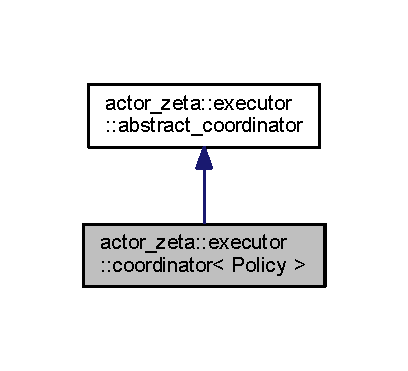
\includegraphics[width=196pt]{classactor__zeta_1_1executor_1_1coordinator__inherit__graph}
\end{center}
\end{figure}


Collaboration diagram for actor\+\_\+zeta\+:\+:executor\+:\+:coordinator$<$ Policy $>$\+:\nopagebreak
\begin{figure}[H]
\begin{center}
\leavevmode
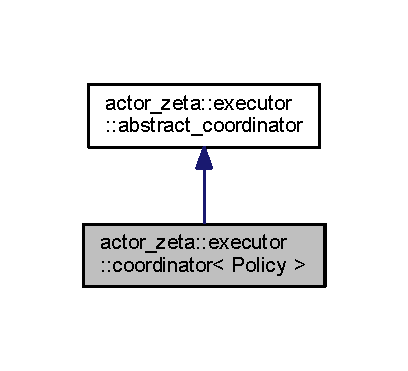
\includegraphics[width=196pt]{classactor__zeta_1_1executor_1_1coordinator__coll__graph}
\end{center}
\end{figure}
\subsection*{Public Types}
\begin{DoxyCompactItemize}
\item 
using \hyperlink{classactor__zeta_1_1executor_1_1coordinator_a6104368cc7f2de545e7c242eda00fcf7}{job\+\_\+ptr} = \hyperlink{structactor__zeta_1_1executor_1_1executable}{executable} $\ast$
\item 
using \hyperlink{classactor__zeta_1_1executor_1_1coordinator_a81ac6921473ebffdc2a20df32249dbcc}{policy\+\_\+data} = typename Policy\+::coordinator\+\_\+data
\item 
using \hyperlink{classactor__zeta_1_1executor_1_1coordinator_a97ba3b1f4578cf25c7311e177edf8c59}{worker\+\_\+type} = \hyperlink{classactor__zeta_1_1executor_1_1worker}{worker}$<$ Policy $>$
\end{DoxyCompactItemize}
\subsection*{Public Member Functions}
\begin{DoxyCompactItemize}
\item 
\hyperlink{classactor__zeta_1_1executor_1_1coordinator_a81ac6921473ebffdc2a20df32249dbcc}{policy\+\_\+data} \& \hyperlink{classactor__zeta_1_1executor_1_1coordinator_a2e94e1b65d78e6c0b0e2861c9b679ddf}{data} ()
\item 
\hyperlink{classactor__zeta_1_1executor_1_1coordinator_a97ba3b1f4578cf25c7311e177edf8c59}{worker\+\_\+type} $\ast$ \hyperlink{classactor__zeta_1_1executor_1_1coordinator_aa008bba1c4e8d94467e79465f978e95b}{worker\+\_\+by\+\_\+id} (size\+\_\+t id)
\item 
void \hyperlink{classactor__zeta_1_1executor_1_1coordinator_a522583023fb9e0c774ca101a09b938f1}{submit} (\hyperlink{classactor__zeta_1_1executor_1_1coordinator_a6104368cc7f2de545e7c242eda00fcf7}{job\+\_\+ptr} job) override
\item 
\hyperlink{classactor__zeta_1_1executor_1_1coordinator_a8775cdb668847488833bf434433971bd}{coordinator} (size\+\_\+t num\+\_\+worker\+\_\+threads, size\+\_\+t max\+\_\+throughput\+\_\+param)
\item 
void \hyperlink{classactor__zeta_1_1executor_1_1coordinator_a1b73b7ddd6b48ba3e15b6f710cb21808}{start} ()
\end{DoxyCompactItemize}


\subsection{Detailed Description}
\subsubsection*{template$<$class Policy$>$\newline
class actor\+\_\+zeta\+::executor\+::coordinator$<$ Policy $>$}

Provides ruler for environment. 


\begin{DoxyTemplParams}{Template Parameters}
{\em Policy} & \\
\hline
\end{DoxyTemplParams}


\subsection{Member Typedef Documentation}
\mbox{\Hypertarget{classactor__zeta_1_1executor_1_1coordinator_a6104368cc7f2de545e7c242eda00fcf7}\label{classactor__zeta_1_1executor_1_1coordinator_a6104368cc7f2de545e7c242eda00fcf7}} 
\index{actor\+\_\+zeta\+::executor\+::coordinator@{actor\+\_\+zeta\+::executor\+::coordinator}!job\+\_\+ptr@{job\+\_\+ptr}}
\index{job\+\_\+ptr@{job\+\_\+ptr}!actor\+\_\+zeta\+::executor\+::coordinator@{actor\+\_\+zeta\+::executor\+::coordinator}}
\subsubsection{\texorpdfstring{job\+\_\+ptr}{job\_ptr}}
{\footnotesize\ttfamily template$<$class Policy $>$ \\
using \hyperlink{classactor__zeta_1_1executor_1_1coordinator}{actor\+\_\+zeta\+::executor\+::coordinator}$<$ Policy $>$\+::\hyperlink{classactor__zeta_1_1executor_1_1coordinator_a6104368cc7f2de545e7c242eda00fcf7}{job\+\_\+ptr} =  \hyperlink{structactor__zeta_1_1executor_1_1executable}{executable} $\ast$}

\mbox{\Hypertarget{classactor__zeta_1_1executor_1_1coordinator_a81ac6921473ebffdc2a20df32249dbcc}\label{classactor__zeta_1_1executor_1_1coordinator_a81ac6921473ebffdc2a20df32249dbcc}} 
\index{actor\+\_\+zeta\+::executor\+::coordinator@{actor\+\_\+zeta\+::executor\+::coordinator}!policy\+\_\+data@{policy\+\_\+data}}
\index{policy\+\_\+data@{policy\+\_\+data}!actor\+\_\+zeta\+::executor\+::coordinator@{actor\+\_\+zeta\+::executor\+::coordinator}}
\subsubsection{\texorpdfstring{policy\+\_\+data}{policy\_data}}
{\footnotesize\ttfamily template$<$class Policy $>$ \\
using \hyperlink{classactor__zeta_1_1executor_1_1coordinator}{actor\+\_\+zeta\+::executor\+::coordinator}$<$ Policy $>$\+::\hyperlink{classactor__zeta_1_1executor_1_1coordinator_a81ac6921473ebffdc2a20df32249dbcc}{policy\+\_\+data} =  typename Policy\+::coordinator\+\_\+data}

\mbox{\Hypertarget{classactor__zeta_1_1executor_1_1coordinator_a97ba3b1f4578cf25c7311e177edf8c59}\label{classactor__zeta_1_1executor_1_1coordinator_a97ba3b1f4578cf25c7311e177edf8c59}} 
\index{actor\+\_\+zeta\+::executor\+::coordinator@{actor\+\_\+zeta\+::executor\+::coordinator}!worker\+\_\+type@{worker\+\_\+type}}
\index{worker\+\_\+type@{worker\+\_\+type}!actor\+\_\+zeta\+::executor\+::coordinator@{actor\+\_\+zeta\+::executor\+::coordinator}}
\subsubsection{\texorpdfstring{worker\+\_\+type}{worker\_type}}
{\footnotesize\ttfamily template$<$class Policy $>$ \\
using \hyperlink{classactor__zeta_1_1executor_1_1coordinator}{actor\+\_\+zeta\+::executor\+::coordinator}$<$ Policy $>$\+::\hyperlink{classactor__zeta_1_1executor_1_1coordinator_a97ba3b1f4578cf25c7311e177edf8c59}{worker\+\_\+type} =  \hyperlink{classactor__zeta_1_1executor_1_1worker}{worker}$<$Policy$>$}



\subsection{Constructor \& Destructor Documentation}
\mbox{\Hypertarget{classactor__zeta_1_1executor_1_1coordinator_a8775cdb668847488833bf434433971bd}\label{classactor__zeta_1_1executor_1_1coordinator_a8775cdb668847488833bf434433971bd}} 
\index{actor\+\_\+zeta\+::executor\+::coordinator@{actor\+\_\+zeta\+::executor\+::coordinator}!coordinator@{coordinator}}
\index{coordinator@{coordinator}!actor\+\_\+zeta\+::executor\+::coordinator@{actor\+\_\+zeta\+::executor\+::coordinator}}
\subsubsection{\texorpdfstring{coordinator()}{coordinator()}}
{\footnotesize\ttfamily template$<$class Policy $>$ \\
\hyperlink{classactor__zeta_1_1executor_1_1coordinator}{actor\+\_\+zeta\+::executor\+::coordinator}$<$ Policy $>$\+::\hyperlink{classactor__zeta_1_1executor_1_1coordinator}{coordinator} (\begin{DoxyParamCaption}\item[{size\+\_\+t}]{num\+\_\+worker\+\_\+threads,  }\item[{size\+\_\+t}]{max\+\_\+throughput\+\_\+param }\end{DoxyParamCaption})\hspace{0.3cm}{\ttfamily [inline]}}



\subsection{Member Function Documentation}
\mbox{\Hypertarget{classactor__zeta_1_1executor_1_1coordinator_a2e94e1b65d78e6c0b0e2861c9b679ddf}\label{classactor__zeta_1_1executor_1_1coordinator_a2e94e1b65d78e6c0b0e2861c9b679ddf}} 
\index{actor\+\_\+zeta\+::executor\+::coordinator@{actor\+\_\+zeta\+::executor\+::coordinator}!data@{data}}
\index{data@{data}!actor\+\_\+zeta\+::executor\+::coordinator@{actor\+\_\+zeta\+::executor\+::coordinator}}
\subsubsection{\texorpdfstring{data()}{data()}}
{\footnotesize\ttfamily template$<$class Policy $>$ \\
\hyperlink{classactor__zeta_1_1executor_1_1coordinator_a81ac6921473ebffdc2a20df32249dbcc}{policy\+\_\+data}\& \hyperlink{classactor__zeta_1_1executor_1_1coordinator}{actor\+\_\+zeta\+::executor\+::coordinator}$<$ Policy $>$\+::data (\begin{DoxyParamCaption}{ }\end{DoxyParamCaption})\hspace{0.3cm}{\ttfamily [inline]}}

\mbox{\Hypertarget{classactor__zeta_1_1executor_1_1coordinator_a1b73b7ddd6b48ba3e15b6f710cb21808}\label{classactor__zeta_1_1executor_1_1coordinator_a1b73b7ddd6b48ba3e15b6f710cb21808}} 
\index{actor\+\_\+zeta\+::executor\+::coordinator@{actor\+\_\+zeta\+::executor\+::coordinator}!start@{start}}
\index{start@{start}!actor\+\_\+zeta\+::executor\+::coordinator@{actor\+\_\+zeta\+::executor\+::coordinator}}
\subsubsection{\texorpdfstring{start()}{start()}}
{\footnotesize\ttfamily template$<$class Policy $>$ \\
void \hyperlink{classactor__zeta_1_1executor_1_1coordinator}{actor\+\_\+zeta\+::executor\+::coordinator}$<$ Policy $>$\+::start (\begin{DoxyParamCaption}{ }\end{DoxyParamCaption})\hspace{0.3cm}{\ttfamily [inline]}, {\ttfamily [virtual]}}



Implements \hyperlink{classactor__zeta_1_1executor_1_1abstract__coordinator_abbbe1a84649a3ae2cfcb60c7728b2944}{actor\+\_\+zeta\+::executor\+::abstract\+\_\+coordinator}.

\mbox{\Hypertarget{classactor__zeta_1_1executor_1_1coordinator_a522583023fb9e0c774ca101a09b938f1}\label{classactor__zeta_1_1executor_1_1coordinator_a522583023fb9e0c774ca101a09b938f1}} 
\index{actor\+\_\+zeta\+::executor\+::coordinator@{actor\+\_\+zeta\+::executor\+::coordinator}!submit@{submit}}
\index{submit@{submit}!actor\+\_\+zeta\+::executor\+::coordinator@{actor\+\_\+zeta\+::executor\+::coordinator}}
\subsubsection{\texorpdfstring{submit()}{submit()}}
{\footnotesize\ttfamily template$<$class Policy $>$ \\
void \hyperlink{classactor__zeta_1_1executor_1_1coordinator}{actor\+\_\+zeta\+::executor\+::coordinator}$<$ Policy $>$\+::submit (\begin{DoxyParamCaption}\item[{\hyperlink{classactor__zeta_1_1executor_1_1coordinator_a6104368cc7f2de545e7c242eda00fcf7}{job\+\_\+ptr}}]{job }\end{DoxyParamCaption})\hspace{0.3cm}{\ttfamily [inline]}, {\ttfamily [override]}}

\mbox{\Hypertarget{classactor__zeta_1_1executor_1_1coordinator_aa008bba1c4e8d94467e79465f978e95b}\label{classactor__zeta_1_1executor_1_1coordinator_aa008bba1c4e8d94467e79465f978e95b}} 
\index{actor\+\_\+zeta\+::executor\+::coordinator@{actor\+\_\+zeta\+::executor\+::coordinator}!worker\+\_\+by\+\_\+id@{worker\+\_\+by\+\_\+id}}
\index{worker\+\_\+by\+\_\+id@{worker\+\_\+by\+\_\+id}!actor\+\_\+zeta\+::executor\+::coordinator@{actor\+\_\+zeta\+::executor\+::coordinator}}
\subsubsection{\texorpdfstring{worker\+\_\+by\+\_\+id()}{worker\_by\_id()}}
{\footnotesize\ttfamily template$<$class Policy $>$ \\
\hyperlink{classactor__zeta_1_1executor_1_1coordinator_a97ba3b1f4578cf25c7311e177edf8c59}{worker\+\_\+type}$\ast$ \hyperlink{classactor__zeta_1_1executor_1_1coordinator}{actor\+\_\+zeta\+::executor\+::coordinator}$<$ Policy $>$\+::worker\+\_\+by\+\_\+id (\begin{DoxyParamCaption}\item[{size\+\_\+t}]{id }\end{DoxyParamCaption})\hspace{0.3cm}{\ttfamily [inline]}}



The documentation for this class was generated from the following file\+:\begin{DoxyCompactItemize}
\item 
\hyperlink{coordinator_8hpp}{coordinator.\+hpp}\end{DoxyCompactItemize}

\hypertarget{structactor__zeta_1_1executor_1_1work__sharing_1_1coordinator__data}{}\section{actor\+\_\+zeta\+:\+:executor\+:\+:work\+\_\+sharing\+:\+:coordinator\+\_\+data Struct Reference}
\label{structactor__zeta_1_1executor_1_1work__sharing_1_1coordinator__data}\index{actor\+\_\+zeta\+::executor\+::work\+\_\+sharing\+::coordinator\+\_\+data@{actor\+\_\+zeta\+::executor\+::work\+\_\+sharing\+::coordinator\+\_\+data}}


This structure is used as coordinator data keeper.  




{\ttfamily \#include $<$work\+\_\+sharing.\+hpp$>$}

\subsection*{Public Member Functions}
\begin{DoxyCompactItemize}
\item 
\hyperlink{structactor__zeta_1_1executor_1_1work__sharing_1_1coordinator__data_afa3541d8688a1f8c0a0377771e3d0e60}{coordinator\+\_\+data} (\hyperlink{classactor__zeta_1_1executor_1_1abstract__coordinator}{executor\+::abstract\+\_\+coordinator} $\ast$)
\end{DoxyCompactItemize}
\subsection*{Public Attributes}
\begin{DoxyCompactItemize}
\item 
\hyperlink{classactor__zeta_1_1executor_1_1work__sharing_a4ed160584612bb4abf7e23ace3590801}{queue\+\_\+type} \hyperlink{structactor__zeta_1_1executor_1_1work__sharing_1_1coordinator__data_ac6dbe15cd908724d0e7e21fb232d2ed9}{queue}
\item 
std\+::mutex \hyperlink{structactor__zeta_1_1executor_1_1work__sharing_1_1coordinator__data_a968512a12d1e853c314092fe036a5731}{lock}
\item 
std\+::condition\+\_\+variable \hyperlink{structactor__zeta_1_1executor_1_1work__sharing_1_1coordinator__data_a0499bb938db7889fb4aa650c7baea21c}{cv}
\end{DoxyCompactItemize}


\subsection{Detailed Description}
This structure is used as coordinator data keeper. 

\subsection{Constructor \& Destructor Documentation}
\mbox{\Hypertarget{structactor__zeta_1_1executor_1_1work__sharing_1_1coordinator__data_afa3541d8688a1f8c0a0377771e3d0e60}\label{structactor__zeta_1_1executor_1_1work__sharing_1_1coordinator__data_afa3541d8688a1f8c0a0377771e3d0e60}} 
\index{actor\+\_\+zeta\+::executor\+::work\+\_\+sharing\+::coordinator\+\_\+data@{actor\+\_\+zeta\+::executor\+::work\+\_\+sharing\+::coordinator\+\_\+data}!coordinator\+\_\+data@{coordinator\+\_\+data}}
\index{coordinator\+\_\+data@{coordinator\+\_\+data}!actor\+\_\+zeta\+::executor\+::work\+\_\+sharing\+::coordinator\+\_\+data@{actor\+\_\+zeta\+::executor\+::work\+\_\+sharing\+::coordinator\+\_\+data}}
\subsubsection{\texorpdfstring{coordinator\+\_\+data()}{coordinator\_data()}}
{\footnotesize\ttfamily actor\+\_\+zeta\+::executor\+::work\+\_\+sharing\+::coordinator\+\_\+data\+::coordinator\+\_\+data (\begin{DoxyParamCaption}\item[{\hyperlink{classactor__zeta_1_1executor_1_1abstract__coordinator}{executor\+::abstract\+\_\+coordinator} $\ast$}]{ }\end{DoxyParamCaption})\hspace{0.3cm}{\ttfamily [inline]}, {\ttfamily [explicit]}}



\subsection{Member Data Documentation}
\mbox{\Hypertarget{structactor__zeta_1_1executor_1_1work__sharing_1_1coordinator__data_a0499bb938db7889fb4aa650c7baea21c}\label{structactor__zeta_1_1executor_1_1work__sharing_1_1coordinator__data_a0499bb938db7889fb4aa650c7baea21c}} 
\index{actor\+\_\+zeta\+::executor\+::work\+\_\+sharing\+::coordinator\+\_\+data@{actor\+\_\+zeta\+::executor\+::work\+\_\+sharing\+::coordinator\+\_\+data}!cv@{cv}}
\index{cv@{cv}!actor\+\_\+zeta\+::executor\+::work\+\_\+sharing\+::coordinator\+\_\+data@{actor\+\_\+zeta\+::executor\+::work\+\_\+sharing\+::coordinator\+\_\+data}}
\subsubsection{\texorpdfstring{cv}{cv}}
{\footnotesize\ttfamily std\+::condition\+\_\+variable actor\+\_\+zeta\+::executor\+::work\+\_\+sharing\+::coordinator\+\_\+data\+::cv}

\mbox{\Hypertarget{structactor__zeta_1_1executor_1_1work__sharing_1_1coordinator__data_a968512a12d1e853c314092fe036a5731}\label{structactor__zeta_1_1executor_1_1work__sharing_1_1coordinator__data_a968512a12d1e853c314092fe036a5731}} 
\index{actor\+\_\+zeta\+::executor\+::work\+\_\+sharing\+::coordinator\+\_\+data@{actor\+\_\+zeta\+::executor\+::work\+\_\+sharing\+::coordinator\+\_\+data}!lock@{lock}}
\index{lock@{lock}!actor\+\_\+zeta\+::executor\+::work\+\_\+sharing\+::coordinator\+\_\+data@{actor\+\_\+zeta\+::executor\+::work\+\_\+sharing\+::coordinator\+\_\+data}}
\subsubsection{\texorpdfstring{lock}{lock}}
{\footnotesize\ttfamily std\+::mutex actor\+\_\+zeta\+::executor\+::work\+\_\+sharing\+::coordinator\+\_\+data\+::lock}

\mbox{\Hypertarget{structactor__zeta_1_1executor_1_1work__sharing_1_1coordinator__data_ac6dbe15cd908724d0e7e21fb232d2ed9}\label{structactor__zeta_1_1executor_1_1work__sharing_1_1coordinator__data_ac6dbe15cd908724d0e7e21fb232d2ed9}} 
\index{actor\+\_\+zeta\+::executor\+::work\+\_\+sharing\+::coordinator\+\_\+data@{actor\+\_\+zeta\+::executor\+::work\+\_\+sharing\+::coordinator\+\_\+data}!queue@{queue}}
\index{queue@{queue}!actor\+\_\+zeta\+::executor\+::work\+\_\+sharing\+::coordinator\+\_\+data@{actor\+\_\+zeta\+::executor\+::work\+\_\+sharing\+::coordinator\+\_\+data}}
\subsubsection{\texorpdfstring{queue}{queue}}
{\footnotesize\ttfamily \hyperlink{classactor__zeta_1_1executor_1_1work__sharing_a4ed160584612bb4abf7e23ace3590801}{queue\+\_\+type} actor\+\_\+zeta\+::executor\+::work\+\_\+sharing\+::coordinator\+\_\+data\+::queue}



The documentation for this struct was generated from the following file\+:\begin{DoxyCompactItemize}
\item 
\hyperlink{work__sharing_8hpp}{work\+\_\+sharing.\+hpp}\end{DoxyCompactItemize}

\hypertarget{classactor__zeta_1_1environment_1_1environment}{}\section{actor\+\_\+zeta\+:\+:environment\+:\+:environment Class Reference}
\label{classactor__zeta_1_1environment_1_1environment}\index{actor\+\_\+zeta\+::environment\+::environment@{actor\+\_\+zeta\+::environment\+::environment}}


An actors workplace platform.  




{\ttfamily \#include $<$environment.\+hpp$>$}



Collaboration diagram for actor\+\_\+zeta\+:\+:environment\+:\+:environment\+:\nopagebreak
\begin{figure}[H]
\begin{center}
\leavevmode
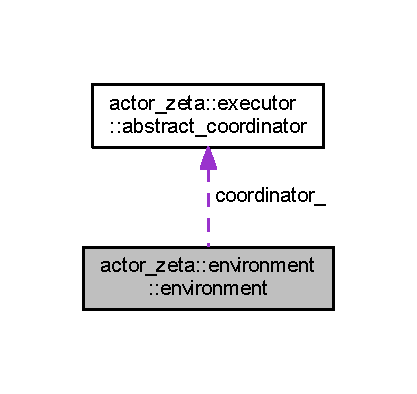
\includegraphics[width=200pt]{classactor__zeta_1_1environment_1_1environment__coll__graph}
\end{center}
\end{figure}
\subsection*{Public Member Functions}
\begin{DoxyCompactItemize}
\item 
\hyperlink{classactor__zeta_1_1environment_1_1environment_a6e6c17cdf01539286c9613b54ac1d4c1}{environment} ()=delete
\item 
\hyperlink{classactor__zeta_1_1environment_1_1environment_a9eae9b55e2d774c0bfaeca8cd5fc77f4}{environment} (const \hyperlink{classactor__zeta_1_1environment_1_1environment}{environment} \&)=delete
\item 
\hyperlink{classactor__zeta_1_1environment_1_1environment}{environment} \& \hyperlink{classactor__zeta_1_1environment_1_1environment_a1ffbad75441e2fe5f65db35df30bb5e7}{operator=} (const \hyperlink{classactor__zeta_1_1environment_1_1environment}{environment} \&)=delete
\item 
\hyperlink{classactor__zeta_1_1environment_1_1environment_a4e2692f38884e10873192f634ba6cfae}{environment} (\hyperlink{classactor__zeta_1_1environment_1_1environment}{environment} \&\&)=default
\item 
\hyperlink{classactor__zeta_1_1environment_1_1environment}{environment} \& \hyperlink{classactor__zeta_1_1environment_1_1environment_a6507409258b8dd2e1629fa6016fc536d}{operator=} (\hyperlink{classactor__zeta_1_1environment_1_1environment}{environment} \&\&)=default
\item 
virtual \hyperlink{classactor__zeta_1_1environment_1_1environment_af8b5af67dbf7a9e05fa1603f239d7a49}{$\sim$environment} ()=default
\item 
virtual int \hyperlink{classactor__zeta_1_1environment_1_1environment_a96929615c4a4acb6ce4aabe9a7a43db9}{start} ()
\item 
\hyperlink{classactor__zeta_1_1environment_1_1environment_a2288101cbca38b4bfc49063e549753eb}{environment} (\hyperlink{classactor__zeta_1_1executor_1_1abstract__coordinator}{executor\+::abstract\+\_\+coordinator} $\ast$)
\item 
\hyperlink{classactor__zeta_1_1executor_1_1abstract__coordinator}{executor\+::abstract\+\_\+coordinator} \& \hyperlink{classactor__zeta_1_1environment_1_1environment_a794484ecbecd03c48214bae1182055f9}{manager\+\_\+execution\+\_\+device} ()
\item 
\hyperlink{classactor__zeta_1_1environment_1_1cooperation}{cooperation} \& \hyperlink{classactor__zeta_1_1environment_1_1environment_ad556eeb7ecd8fcd6337e2af39e57ce9e}{manager\+\_\+group} ()
\end{DoxyCompactItemize}
\subsection*{Protected Attributes}
\begin{DoxyCompactItemize}
\item 
\hyperlink{classactor__zeta_1_1executor_1_1abstract__coordinator}{executor\+::abstract\+\_\+coordinator} $\ast$ \hyperlink{classactor__zeta_1_1environment_1_1environment_a9c6ddfd97b9fa631d6c3a2385bec9581}{coordinator\+\_\+}
\end{DoxyCompactItemize}


\subsection{Detailed Description}
An actors workplace platform. 

\subsection{Constructor \& Destructor Documentation}
\mbox{\Hypertarget{classactor__zeta_1_1environment_1_1environment_a6e6c17cdf01539286c9613b54ac1d4c1}\label{classactor__zeta_1_1environment_1_1environment_a6e6c17cdf01539286c9613b54ac1d4c1}} 
\index{actor\+\_\+zeta\+::environment\+::environment@{actor\+\_\+zeta\+::environment\+::environment}!environment@{environment}}
\index{environment@{environment}!actor\+\_\+zeta\+::environment\+::environment@{actor\+\_\+zeta\+::environment\+::environment}}
\subsubsection{\texorpdfstring{environment()}{environment()}\hspace{0.1cm}{\footnotesize\ttfamily [1/4]}}
{\footnotesize\ttfamily actor\+\_\+zeta\+::environment\+::environment\+::environment (\begin{DoxyParamCaption}{ }\end{DoxyParamCaption})\hspace{0.3cm}{\ttfamily [delete]}}

\mbox{\Hypertarget{classactor__zeta_1_1environment_1_1environment_a9eae9b55e2d774c0bfaeca8cd5fc77f4}\label{classactor__zeta_1_1environment_1_1environment_a9eae9b55e2d774c0bfaeca8cd5fc77f4}} 
\index{actor\+\_\+zeta\+::environment\+::environment@{actor\+\_\+zeta\+::environment\+::environment}!environment@{environment}}
\index{environment@{environment}!actor\+\_\+zeta\+::environment\+::environment@{actor\+\_\+zeta\+::environment\+::environment}}
\subsubsection{\texorpdfstring{environment()}{environment()}\hspace{0.1cm}{\footnotesize\ttfamily [2/4]}}
{\footnotesize\ttfamily actor\+\_\+zeta\+::environment\+::environment\+::environment (\begin{DoxyParamCaption}\item[{const \hyperlink{classactor__zeta_1_1environment_1_1environment}{environment} \&}]{ }\end{DoxyParamCaption})\hspace{0.3cm}{\ttfamily [delete]}}

\mbox{\Hypertarget{classactor__zeta_1_1environment_1_1environment_a4e2692f38884e10873192f634ba6cfae}\label{classactor__zeta_1_1environment_1_1environment_a4e2692f38884e10873192f634ba6cfae}} 
\index{actor\+\_\+zeta\+::environment\+::environment@{actor\+\_\+zeta\+::environment\+::environment}!environment@{environment}}
\index{environment@{environment}!actor\+\_\+zeta\+::environment\+::environment@{actor\+\_\+zeta\+::environment\+::environment}}
\subsubsection{\texorpdfstring{environment()}{environment()}\hspace{0.1cm}{\footnotesize\ttfamily [3/4]}}
{\footnotesize\ttfamily actor\+\_\+zeta\+::environment\+::environment\+::environment (\begin{DoxyParamCaption}\item[{\hyperlink{classactor__zeta_1_1environment_1_1environment}{environment} \&\&}]{ }\end{DoxyParamCaption})\hspace{0.3cm}{\ttfamily [default]}}

\mbox{\Hypertarget{classactor__zeta_1_1environment_1_1environment_af8b5af67dbf7a9e05fa1603f239d7a49}\label{classactor__zeta_1_1environment_1_1environment_af8b5af67dbf7a9e05fa1603f239d7a49}} 
\index{actor\+\_\+zeta\+::environment\+::environment@{actor\+\_\+zeta\+::environment\+::environment}!````~environment@{$\sim$environment}}
\index{````~environment@{$\sim$environment}!actor\+\_\+zeta\+::environment\+::environment@{actor\+\_\+zeta\+::environment\+::environment}}
\subsubsection{\texorpdfstring{$\sim$environment()}{~environment()}}
{\footnotesize\ttfamily virtual actor\+\_\+zeta\+::environment\+::environment\+::$\sim$environment (\begin{DoxyParamCaption}{ }\end{DoxyParamCaption})\hspace{0.3cm}{\ttfamily [virtual]}, {\ttfamily [default]}}

\mbox{\Hypertarget{classactor__zeta_1_1environment_1_1environment_a2288101cbca38b4bfc49063e549753eb}\label{classactor__zeta_1_1environment_1_1environment_a2288101cbca38b4bfc49063e549753eb}} 
\index{actor\+\_\+zeta\+::environment\+::environment@{actor\+\_\+zeta\+::environment\+::environment}!environment@{environment}}
\index{environment@{environment}!actor\+\_\+zeta\+::environment\+::environment@{actor\+\_\+zeta\+::environment\+::environment}}
\subsubsection{\texorpdfstring{environment()}{environment()}\hspace{0.1cm}{\footnotesize\ttfamily [4/4]}}
{\footnotesize\ttfamily actor\+\_\+zeta\+::environment\+::environment\+::environment (\begin{DoxyParamCaption}\item[{\hyperlink{classactor__zeta_1_1executor_1_1abstract__coordinator}{executor\+::abstract\+\_\+coordinator} $\ast$}]{ac }\end{DoxyParamCaption})}



\subsection{Member Function Documentation}
\mbox{\Hypertarget{classactor__zeta_1_1environment_1_1environment_a794484ecbecd03c48214bae1182055f9}\label{classactor__zeta_1_1environment_1_1environment_a794484ecbecd03c48214bae1182055f9}} 
\index{actor\+\_\+zeta\+::environment\+::environment@{actor\+\_\+zeta\+::environment\+::environment}!manager\+\_\+execution\+\_\+device@{manager\+\_\+execution\+\_\+device}}
\index{manager\+\_\+execution\+\_\+device@{manager\+\_\+execution\+\_\+device}!actor\+\_\+zeta\+::environment\+::environment@{actor\+\_\+zeta\+::environment\+::environment}}
\subsubsection{\texorpdfstring{manager\+\_\+execution\+\_\+device()}{manager\_execution\_device()}}
{\footnotesize\ttfamily \hyperlink{classactor__zeta_1_1executor_1_1abstract__coordinator}{executor\+::abstract\+\_\+coordinator} \& actor\+\_\+zeta\+::environment\+::environment\+::manager\+\_\+execution\+\_\+device (\begin{DoxyParamCaption}{ }\end{DoxyParamCaption})}

\mbox{\Hypertarget{classactor__zeta_1_1environment_1_1environment_ad556eeb7ecd8fcd6337e2af39e57ce9e}\label{classactor__zeta_1_1environment_1_1environment_ad556eeb7ecd8fcd6337e2af39e57ce9e}} 
\index{actor\+\_\+zeta\+::environment\+::environment@{actor\+\_\+zeta\+::environment\+::environment}!manager\+\_\+group@{manager\+\_\+group}}
\index{manager\+\_\+group@{manager\+\_\+group}!actor\+\_\+zeta\+::environment\+::environment@{actor\+\_\+zeta\+::environment\+::environment}}
\subsubsection{\texorpdfstring{manager\+\_\+group()}{manager\_group()}}
{\footnotesize\ttfamily \hyperlink{classactor__zeta_1_1environment_1_1cooperation}{cooperation} \& actor\+\_\+zeta\+::environment\+::environment\+::manager\+\_\+group (\begin{DoxyParamCaption}{ }\end{DoxyParamCaption})}

\mbox{\Hypertarget{classactor__zeta_1_1environment_1_1environment_a1ffbad75441e2fe5f65db35df30bb5e7}\label{classactor__zeta_1_1environment_1_1environment_a1ffbad75441e2fe5f65db35df30bb5e7}} 
\index{actor\+\_\+zeta\+::environment\+::environment@{actor\+\_\+zeta\+::environment\+::environment}!operator=@{operator=}}
\index{operator=@{operator=}!actor\+\_\+zeta\+::environment\+::environment@{actor\+\_\+zeta\+::environment\+::environment}}
\subsubsection{\texorpdfstring{operator=()}{operator=()}\hspace{0.1cm}{\footnotesize\ttfamily [1/2]}}
{\footnotesize\ttfamily \hyperlink{classactor__zeta_1_1environment_1_1environment}{environment}\& actor\+\_\+zeta\+::environment\+::environment\+::operator= (\begin{DoxyParamCaption}\item[{const \hyperlink{classactor__zeta_1_1environment_1_1environment}{environment} \&}]{ }\end{DoxyParamCaption})\hspace{0.3cm}{\ttfamily [delete]}}

\mbox{\Hypertarget{classactor__zeta_1_1environment_1_1environment_a6507409258b8dd2e1629fa6016fc536d}\label{classactor__zeta_1_1environment_1_1environment_a6507409258b8dd2e1629fa6016fc536d}} 
\index{actor\+\_\+zeta\+::environment\+::environment@{actor\+\_\+zeta\+::environment\+::environment}!operator=@{operator=}}
\index{operator=@{operator=}!actor\+\_\+zeta\+::environment\+::environment@{actor\+\_\+zeta\+::environment\+::environment}}
\subsubsection{\texorpdfstring{operator=()}{operator=()}\hspace{0.1cm}{\footnotesize\ttfamily [2/2]}}
{\footnotesize\ttfamily \hyperlink{classactor__zeta_1_1environment_1_1environment}{environment}\& actor\+\_\+zeta\+::environment\+::environment\+::operator= (\begin{DoxyParamCaption}\item[{\hyperlink{classactor__zeta_1_1environment_1_1environment}{environment} \&\&}]{ }\end{DoxyParamCaption})\hspace{0.3cm}{\ttfamily [default]}}

\mbox{\Hypertarget{classactor__zeta_1_1environment_1_1environment_a96929615c4a4acb6ce4aabe9a7a43db9}\label{classactor__zeta_1_1environment_1_1environment_a96929615c4a4acb6ce4aabe9a7a43db9}} 
\index{actor\+\_\+zeta\+::environment\+::environment@{actor\+\_\+zeta\+::environment\+::environment}!start@{start}}
\index{start@{start}!actor\+\_\+zeta\+::environment\+::environment@{actor\+\_\+zeta\+::environment\+::environment}}
\subsubsection{\texorpdfstring{start()}{start()}}
{\footnotesize\ttfamily int actor\+\_\+zeta\+::environment\+::environment\+::start (\begin{DoxyParamCaption}{ }\end{DoxyParamCaption})\hspace{0.3cm}{\ttfamily [virtual]}}



\subsection{Member Data Documentation}
\mbox{\Hypertarget{classactor__zeta_1_1environment_1_1environment_a9c6ddfd97b9fa631d6c3a2385bec9581}\label{classactor__zeta_1_1environment_1_1environment_a9c6ddfd97b9fa631d6c3a2385bec9581}} 
\index{actor\+\_\+zeta\+::environment\+::environment@{actor\+\_\+zeta\+::environment\+::environment}!coordinator\+\_\+@{coordinator\+\_\+}}
\index{coordinator\+\_\+@{coordinator\+\_\+}!actor\+\_\+zeta\+::environment\+::environment@{actor\+\_\+zeta\+::environment\+::environment}}
\subsubsection{\texorpdfstring{coordinator\+\_\+}{coordinator\_}}
{\footnotesize\ttfamily \hyperlink{classactor__zeta_1_1executor_1_1abstract__coordinator}{executor\+::abstract\+\_\+coordinator}$\ast$ actor\+\_\+zeta\+::environment\+::environment\+::coordinator\+\_\+\hspace{0.3cm}{\ttfamily [protected]}}



The documentation for this class was generated from the following files\+:\begin{DoxyCompactItemize}
\item 
\hyperlink{environment_8hpp}{environment.\+hpp}\item 
\hyperlink{environment_8cpp}{environment.\+cpp}\end{DoxyCompactItemize}

\hypertarget{structactor__zeta_1_1executor_1_1executable}{}\section{actor\+\_\+zeta\+:\+:executor\+:\+:executable Struct Reference}
\label{structactor__zeta_1_1executor_1_1executable}\index{actor\+\_\+zeta\+::executor\+::executable@{actor\+\_\+zeta\+::executor\+::executable}}


{\ttfamily \#include $<$executable.\+hpp$>$}



Inheritance diagram for actor\+\_\+zeta\+:\+:executor\+:\+:executable\+:\nopagebreak
\begin{figure}[H]
\begin{center}
\leavevmode
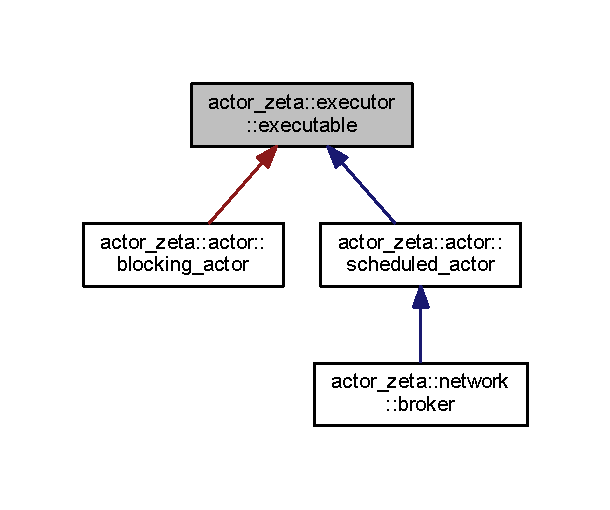
\includegraphics[width=293pt]{structactor__zeta_1_1executor_1_1executable__inherit__graph}
\end{center}
\end{figure}
\subsection*{Public Types}
\begin{DoxyCompactItemize}
\item 
enum \hyperlink{structactor__zeta_1_1executor_1_1executable_aef06c63be7b22b021ade4b83ed4f3cc4}{executable\+\_\+result} \{ \hyperlink{structactor__zeta_1_1executor_1_1executable_aef06c63be7b22b021ade4b83ed4f3cc4a69f2afc2390cec954f7c208b07212d39}{executable\+\_\+result\+::resume}, 
\hyperlink{structactor__zeta_1_1executor_1_1executable_aef06c63be7b22b021ade4b83ed4f3cc4a3ef2b55c41ed0d65d1e18c3ed461b5a7}{executable\+\_\+result\+::awaiting}, 
\hyperlink{structactor__zeta_1_1executor_1_1executable_aef06c63be7b22b021ade4b83ed4f3cc4a6b2ded51d81a4403d8a4bd25fa1e57ee}{executable\+\_\+result\+::done}, 
\hyperlink{structactor__zeta_1_1executor_1_1executable_aef06c63be7b22b021ade4b83ed4f3cc4a5924f03a95ee6f7277e5bdd1e81b8fdc}{executable\+\_\+result\+::shutdown}
 \}
\end{DoxyCompactItemize}
\subsection*{Public Member Functions}
\begin{DoxyCompactItemize}
\item 
virtual \hyperlink{structactor__zeta_1_1executor_1_1executable_a12fbe24c0d826dbeae7ee3f9cae4ccf5}{$\sim$executable} ()=default
\item 
virtual void \hyperlink{structactor__zeta_1_1executor_1_1executable_a35557044e3f8d17504a66628aeea1cee}{attach\+\_\+to\+\_\+scheduler} ()=0
\item 
virtual void \hyperlink{structactor__zeta_1_1executor_1_1executable_a2fe91b45b919fc6f3fce21e64d2c1f91}{detach\+\_\+from\+\_\+scheduler} ()=0
\item 
virtual \hyperlink{structactor__zeta_1_1executor_1_1executable_aef06c63be7b22b021ade4b83ed4f3cc4}{executable\+\_\+result} \hyperlink{structactor__zeta_1_1executor_1_1executable_a61d6cbce8b124e1e5ef80f8befea2a89}{run} (\hyperlink{structactor__zeta_1_1executor_1_1execution__device}{executor\+::execution\+\_\+device} $\ast$, size\+\_\+t max\+\_\+throughput)=0
\end{DoxyCompactItemize}


\subsection{Member Enumeration Documentation}
\mbox{\Hypertarget{structactor__zeta_1_1executor_1_1executable_aef06c63be7b22b021ade4b83ed4f3cc4}\label{structactor__zeta_1_1executor_1_1executable_aef06c63be7b22b021ade4b83ed4f3cc4}} 
\index{actor\+\_\+zeta\+::executor\+::executable@{actor\+\_\+zeta\+::executor\+::executable}!executable\+\_\+result@{executable\+\_\+result}}
\index{executable\+\_\+result@{executable\+\_\+result}!actor\+\_\+zeta\+::executor\+::executable@{actor\+\_\+zeta\+::executor\+::executable}}
\subsubsection{\texorpdfstring{executable\+\_\+result}{executable\_result}}
{\footnotesize\ttfamily enum \hyperlink{structactor__zeta_1_1executor_1_1executable_aef06c63be7b22b021ade4b83ed4f3cc4}{actor\+\_\+zeta\+::executor\+::executable\+::executable\+\_\+result}\hspace{0.3cm}{\ttfamily [strong]}}

\begin{DoxyEnumFields}{Enumerator}
\raisebox{\heightof{T}}[0pt][0pt]{\index{resume@{resume}!actor\+\_\+zeta\+::executor\+::executable@{actor\+\_\+zeta\+::executor\+::executable}}\index{actor\+\_\+zeta\+::executor\+::executable@{actor\+\_\+zeta\+::executor\+::executable}!resume@{resume}}}\mbox{\Hypertarget{structactor__zeta_1_1executor_1_1executable_aef06c63be7b22b021ade4b83ed4f3cc4a69f2afc2390cec954f7c208b07212d39}\label{structactor__zeta_1_1executor_1_1executable_aef06c63be7b22b021ade4b83ed4f3cc4a69f2afc2390cec954f7c208b07212d39}} 
resume&is coded as std\+::int of value 0 \\
\hline

\raisebox{\heightof{T}}[0pt][0pt]{\index{awaiting@{awaiting}!actor\+\_\+zeta\+::executor\+::executable@{actor\+\_\+zeta\+::executor\+::executable}}\index{actor\+\_\+zeta\+::executor\+::executable@{actor\+\_\+zeta\+::executor\+::executable}!awaiting@{awaiting}}}\mbox{\Hypertarget{structactor__zeta_1_1executor_1_1executable_aef06c63be7b22b021ade4b83ed4f3cc4a3ef2b55c41ed0d65d1e18c3ed461b5a7}\label{structactor__zeta_1_1executor_1_1executable_aef06c63be7b22b021ade4b83ed4f3cc4a3ef2b55c41ed0d65d1e18c3ed461b5a7}} 
awaiting&is coded as std\+::int of value 1 \\
\hline

\raisebox{\heightof{T}}[0pt][0pt]{\index{done@{done}!actor\+\_\+zeta\+::executor\+::executable@{actor\+\_\+zeta\+::executor\+::executable}}\index{actor\+\_\+zeta\+::executor\+::executable@{actor\+\_\+zeta\+::executor\+::executable}!done@{done}}}\mbox{\Hypertarget{structactor__zeta_1_1executor_1_1executable_aef06c63be7b22b021ade4b83ed4f3cc4a6b2ded51d81a4403d8a4bd25fa1e57ee}\label{structactor__zeta_1_1executor_1_1executable_aef06c63be7b22b021ade4b83ed4f3cc4a6b2ded51d81a4403d8a4bd25fa1e57ee}} 
done&is coded as std\+::int of value 2 \\
\hline

\raisebox{\heightof{T}}[0pt][0pt]{\index{shutdown@{shutdown}!actor\+\_\+zeta\+::executor\+::executable@{actor\+\_\+zeta\+::executor\+::executable}}\index{actor\+\_\+zeta\+::executor\+::executable@{actor\+\_\+zeta\+::executor\+::executable}!shutdown@{shutdown}}}\mbox{\Hypertarget{structactor__zeta_1_1executor_1_1executable_aef06c63be7b22b021ade4b83ed4f3cc4a5924f03a95ee6f7277e5bdd1e81b8fdc}\label{structactor__zeta_1_1executor_1_1executable_aef06c63be7b22b021ade4b83ed4f3cc4a5924f03a95ee6f7277e5bdd1e81b8fdc}} 
shutdown&is coded as std\+::int of value 3 \\
\hline

\end{DoxyEnumFields}


\subsection{Constructor \& Destructor Documentation}
\mbox{\Hypertarget{structactor__zeta_1_1executor_1_1executable_a12fbe24c0d826dbeae7ee3f9cae4ccf5}\label{structactor__zeta_1_1executor_1_1executable_a12fbe24c0d826dbeae7ee3f9cae4ccf5}} 
\index{actor\+\_\+zeta\+::executor\+::executable@{actor\+\_\+zeta\+::executor\+::executable}!````~executable@{$\sim$executable}}
\index{````~executable@{$\sim$executable}!actor\+\_\+zeta\+::executor\+::executable@{actor\+\_\+zeta\+::executor\+::executable}}
\subsubsection{\texorpdfstring{$\sim$executable()}{~executable()}}
{\footnotesize\ttfamily virtual actor\+\_\+zeta\+::executor\+::executable\+::$\sim$executable (\begin{DoxyParamCaption}{ }\end{DoxyParamCaption})\hspace{0.3cm}{\ttfamily [virtual]}, {\ttfamily [default]}}



\subsection{Member Function Documentation}
\mbox{\Hypertarget{structactor__zeta_1_1executor_1_1executable_a35557044e3f8d17504a66628aeea1cee}\label{structactor__zeta_1_1executor_1_1executable_a35557044e3f8d17504a66628aeea1cee}} 
\index{actor\+\_\+zeta\+::executor\+::executable@{actor\+\_\+zeta\+::executor\+::executable}!attach\+\_\+to\+\_\+scheduler@{attach\+\_\+to\+\_\+scheduler}}
\index{attach\+\_\+to\+\_\+scheduler@{attach\+\_\+to\+\_\+scheduler}!actor\+\_\+zeta\+::executor\+::executable@{actor\+\_\+zeta\+::executor\+::executable}}
\subsubsection{\texorpdfstring{attach\+\_\+to\+\_\+scheduler()}{attach\_to\_scheduler()}}
{\footnotesize\ttfamily virtual void actor\+\_\+zeta\+::executor\+::executable\+::attach\+\_\+to\+\_\+scheduler (\begin{DoxyParamCaption}{ }\end{DoxyParamCaption})\hspace{0.3cm}{\ttfamily [pure virtual]}}



Implemented in \hyperlink{classactor__zeta_1_1actor_1_1scheduled__actor_a760f7fedcd61cae392c435a13bcab50c}{actor\+\_\+zeta\+::actor\+::scheduled\+\_\+actor}.

\mbox{\Hypertarget{structactor__zeta_1_1executor_1_1executable_a2fe91b45b919fc6f3fce21e64d2c1f91}\label{structactor__zeta_1_1executor_1_1executable_a2fe91b45b919fc6f3fce21e64d2c1f91}} 
\index{actor\+\_\+zeta\+::executor\+::executable@{actor\+\_\+zeta\+::executor\+::executable}!detach\+\_\+from\+\_\+scheduler@{detach\+\_\+from\+\_\+scheduler}}
\index{detach\+\_\+from\+\_\+scheduler@{detach\+\_\+from\+\_\+scheduler}!actor\+\_\+zeta\+::executor\+::executable@{actor\+\_\+zeta\+::executor\+::executable}}
\subsubsection{\texorpdfstring{detach\+\_\+from\+\_\+scheduler()}{detach\_from\_scheduler()}}
{\footnotesize\ttfamily virtual void actor\+\_\+zeta\+::executor\+::executable\+::detach\+\_\+from\+\_\+scheduler (\begin{DoxyParamCaption}{ }\end{DoxyParamCaption})\hspace{0.3cm}{\ttfamily [pure virtual]}}



Implemented in \hyperlink{classactor__zeta_1_1actor_1_1scheduled__actor_aaf6582fc27718071ff7c9d516b8f0cf6}{actor\+\_\+zeta\+::actor\+::scheduled\+\_\+actor}.

\mbox{\Hypertarget{structactor__zeta_1_1executor_1_1executable_a61d6cbce8b124e1e5ef80f8befea2a89}\label{structactor__zeta_1_1executor_1_1executable_a61d6cbce8b124e1e5ef80f8befea2a89}} 
\index{actor\+\_\+zeta\+::executor\+::executable@{actor\+\_\+zeta\+::executor\+::executable}!run@{run}}
\index{run@{run}!actor\+\_\+zeta\+::executor\+::executable@{actor\+\_\+zeta\+::executor\+::executable}}
\subsubsection{\texorpdfstring{run()}{run()}}
{\footnotesize\ttfamily virtual \hyperlink{structactor__zeta_1_1executor_1_1executable_aef06c63be7b22b021ade4b83ed4f3cc4}{executable\+\_\+result} actor\+\_\+zeta\+::executor\+::executable\+::run (\begin{DoxyParamCaption}\item[{\hyperlink{structactor__zeta_1_1executor_1_1execution__device}{executor\+::execution\+\_\+device} $\ast$}]{,  }\item[{size\+\_\+t}]{max\+\_\+throughput }\end{DoxyParamCaption})\hspace{0.3cm}{\ttfamily [pure virtual]}}



Implemented in \hyperlink{classactor__zeta_1_1actor_1_1scheduled__actor_a9031c2f3ff6c8c62698b53fa92e56274}{actor\+\_\+zeta\+::actor\+::scheduled\+\_\+actor}, and \hyperlink{classactor__zeta_1_1actor_1_1blocking__actor_af92ae4139344b002f8014433f64f8e56}{actor\+\_\+zeta\+::actor\+::blocking\+\_\+actor}.



The documentation for this struct was generated from the following file\+:\begin{DoxyCompactItemize}
\item 
\hyperlink{executable_8hpp}{executable.\+hpp}\end{DoxyCompactItemize}

\hypertarget{structactor__zeta_1_1executor_1_1execution__device}{}\section{actor\+\_\+zeta\+:\+:executor\+:\+:execution\+\_\+device Struct Reference}
\label{structactor__zeta_1_1executor_1_1execution__device}\index{actor\+\_\+zeta\+::executor\+::execution\+\_\+device@{actor\+\_\+zeta\+::executor\+::execution\+\_\+device}}


\hyperlink{structactor__zeta_1_1executor_1_1execution__device}{execution\+\_\+device}  




{\ttfamily \#include $<$execution\+\_\+device.\+hpp$>$}



Inheritance diagram for actor\+\_\+zeta\+:\+:executor\+:\+:execution\+\_\+device\+:\nopagebreak
\begin{figure}[H]
\begin{center}
\leavevmode
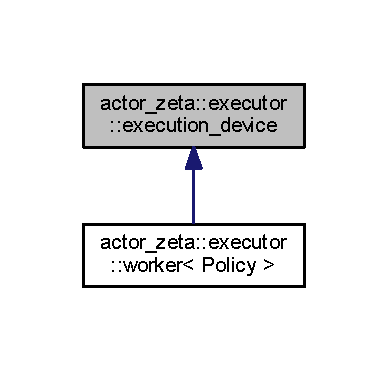
\includegraphics[width=186pt]{structactor__zeta_1_1executor_1_1execution__device__inherit__graph}
\end{center}
\end{figure}
\subsection*{Public Member Functions}
\begin{DoxyCompactItemize}
\item 
\hyperlink{structactor__zeta_1_1executor_1_1execution__device_a552c067e38d17da26a4b2f41db21db3d}{execution\+\_\+device} ()=default
\item 
\hyperlink{structactor__zeta_1_1executor_1_1execution__device_a4d17ed7f7479e2c49dd6a373ca2bf8b1}{execution\+\_\+device} (\hyperlink{structactor__zeta_1_1executor_1_1execution__device}{execution\+\_\+device} \&\&)=delete
\item 
\hyperlink{structactor__zeta_1_1executor_1_1execution__device_a21ece5bd6bc0cc1ce608f6b9eaa7a49b}{execution\+\_\+device} (const \hyperlink{structactor__zeta_1_1executor_1_1execution__device}{execution\+\_\+device} \&)=delete
\item 
virtual \hyperlink{structactor__zeta_1_1executor_1_1execution__device_a4079ca9f4b13fe247c9da029a7c3a351}{$\sim$execution\+\_\+device} ()=default
\item 
virtual void \hyperlink{structactor__zeta_1_1executor_1_1execution__device_a9e6a0a577c4b85e16af82f228e9612eb}{put\+\_\+execute\+\_\+latest} (\hyperlink{structactor__zeta_1_1executor_1_1executable}{executable} $\ast$)=0
\end{DoxyCompactItemize}


\subsection{Detailed Description}
\hyperlink{structactor__zeta_1_1executor_1_1execution__device}{execution\+\_\+device} 

\subsection{Constructor \& Destructor Documentation}
\mbox{\Hypertarget{structactor__zeta_1_1executor_1_1execution__device_a552c067e38d17da26a4b2f41db21db3d}\label{structactor__zeta_1_1executor_1_1execution__device_a552c067e38d17da26a4b2f41db21db3d}} 
\index{actor\+\_\+zeta\+::executor\+::execution\+\_\+device@{actor\+\_\+zeta\+::executor\+::execution\+\_\+device}!execution\+\_\+device@{execution\+\_\+device}}
\index{execution\+\_\+device@{execution\+\_\+device}!actor\+\_\+zeta\+::executor\+::execution\+\_\+device@{actor\+\_\+zeta\+::executor\+::execution\+\_\+device}}
\subsubsection{\texorpdfstring{execution\+\_\+device()}{execution\_device()}\hspace{0.1cm}{\footnotesize\ttfamily [1/3]}}
{\footnotesize\ttfamily actor\+\_\+zeta\+::executor\+::execution\+\_\+device\+::execution\+\_\+device (\begin{DoxyParamCaption}{ }\end{DoxyParamCaption})\hspace{0.3cm}{\ttfamily [default]}}

\mbox{\Hypertarget{structactor__zeta_1_1executor_1_1execution__device_a4d17ed7f7479e2c49dd6a373ca2bf8b1}\label{structactor__zeta_1_1executor_1_1execution__device_a4d17ed7f7479e2c49dd6a373ca2bf8b1}} 
\index{actor\+\_\+zeta\+::executor\+::execution\+\_\+device@{actor\+\_\+zeta\+::executor\+::execution\+\_\+device}!execution\+\_\+device@{execution\+\_\+device}}
\index{execution\+\_\+device@{execution\+\_\+device}!actor\+\_\+zeta\+::executor\+::execution\+\_\+device@{actor\+\_\+zeta\+::executor\+::execution\+\_\+device}}
\subsubsection{\texorpdfstring{execution\+\_\+device()}{execution\_device()}\hspace{0.1cm}{\footnotesize\ttfamily [2/3]}}
{\footnotesize\ttfamily actor\+\_\+zeta\+::executor\+::execution\+\_\+device\+::execution\+\_\+device (\begin{DoxyParamCaption}\item[{\hyperlink{structactor__zeta_1_1executor_1_1execution__device}{execution\+\_\+device} \&\&}]{ }\end{DoxyParamCaption})\hspace{0.3cm}{\ttfamily [delete]}}

\mbox{\Hypertarget{structactor__zeta_1_1executor_1_1execution__device_a21ece5bd6bc0cc1ce608f6b9eaa7a49b}\label{structactor__zeta_1_1executor_1_1execution__device_a21ece5bd6bc0cc1ce608f6b9eaa7a49b}} 
\index{actor\+\_\+zeta\+::executor\+::execution\+\_\+device@{actor\+\_\+zeta\+::executor\+::execution\+\_\+device}!execution\+\_\+device@{execution\+\_\+device}}
\index{execution\+\_\+device@{execution\+\_\+device}!actor\+\_\+zeta\+::executor\+::execution\+\_\+device@{actor\+\_\+zeta\+::executor\+::execution\+\_\+device}}
\subsubsection{\texorpdfstring{execution\+\_\+device()}{execution\_device()}\hspace{0.1cm}{\footnotesize\ttfamily [3/3]}}
{\footnotesize\ttfamily actor\+\_\+zeta\+::executor\+::execution\+\_\+device\+::execution\+\_\+device (\begin{DoxyParamCaption}\item[{const \hyperlink{structactor__zeta_1_1executor_1_1execution__device}{execution\+\_\+device} \&}]{ }\end{DoxyParamCaption})\hspace{0.3cm}{\ttfamily [delete]}}

\mbox{\Hypertarget{structactor__zeta_1_1executor_1_1execution__device_a4079ca9f4b13fe247c9da029a7c3a351}\label{structactor__zeta_1_1executor_1_1execution__device_a4079ca9f4b13fe247c9da029a7c3a351}} 
\index{actor\+\_\+zeta\+::executor\+::execution\+\_\+device@{actor\+\_\+zeta\+::executor\+::execution\+\_\+device}!````~execution\+\_\+device@{$\sim$execution\+\_\+device}}
\index{````~execution\+\_\+device@{$\sim$execution\+\_\+device}!actor\+\_\+zeta\+::executor\+::execution\+\_\+device@{actor\+\_\+zeta\+::executor\+::execution\+\_\+device}}
\subsubsection{\texorpdfstring{$\sim$execution\+\_\+device()}{~execution\_device()}}
{\footnotesize\ttfamily virtual actor\+\_\+zeta\+::executor\+::execution\+\_\+device\+::$\sim$execution\+\_\+device (\begin{DoxyParamCaption}{ }\end{DoxyParamCaption})\hspace{0.3cm}{\ttfamily [virtual]}, {\ttfamily [default]}}



\subsection{Member Function Documentation}
\mbox{\Hypertarget{structactor__zeta_1_1executor_1_1execution__device_a9e6a0a577c4b85e16af82f228e9612eb}\label{structactor__zeta_1_1executor_1_1execution__device_a9e6a0a577c4b85e16af82f228e9612eb}} 
\index{actor\+\_\+zeta\+::executor\+::execution\+\_\+device@{actor\+\_\+zeta\+::executor\+::execution\+\_\+device}!put\+\_\+execute\+\_\+latest@{put\+\_\+execute\+\_\+latest}}
\index{put\+\_\+execute\+\_\+latest@{put\+\_\+execute\+\_\+latest}!actor\+\_\+zeta\+::executor\+::execution\+\_\+device@{actor\+\_\+zeta\+::executor\+::execution\+\_\+device}}
\subsubsection{\texorpdfstring{put\+\_\+execute\+\_\+latest()}{put\_execute\_latest()}}
{\footnotesize\ttfamily virtual void actor\+\_\+zeta\+::executor\+::execution\+\_\+device\+::put\+\_\+execute\+\_\+latest (\begin{DoxyParamCaption}\item[{\hyperlink{structactor__zeta_1_1executor_1_1executable}{executable} $\ast$}]{ }\end{DoxyParamCaption})\hspace{0.3cm}{\ttfamily [pure virtual]}}



The documentation for this struct was generated from the following file\+:\begin{DoxyCompactItemize}
\item 
\hyperlink{execution__device_8hpp}{execution\+\_\+device.\+hpp}\end{DoxyCompactItemize}

\hypertarget{classactor__zeta_1_1environment_1_1group}{}\section{actor\+\_\+zeta\+:\+:environment\+:\+:group Class Reference}
\label{classactor__zeta_1_1environment_1_1group}\index{actor\+\_\+zeta\+::environment\+::group@{actor\+\_\+zeta\+::environment\+::group}}


A group combinator for actors.  




{\ttfamily \#include $<$group.\+hpp$>$}

\subsection*{Public Member Functions}
\begin{DoxyCompactItemize}
\item 
\hyperlink{classactor__zeta_1_1environment_1_1group_a406f197675df3a610f7f1f97d618fd8b}{group} ()=default
\item 
\hyperlink{classactor__zeta_1_1environment_1_1group_a128770ca8d096ecc83261e2fb4be84f4}{group} (const \hyperlink{classactor__zeta_1_1environment_1_1group}{group} \&)=delete
\item 
\hyperlink{classactor__zeta_1_1environment_1_1group_a653e9b9e4ecd7ec5fb859d8bab0af7ef}{group} (\hyperlink{classactor__zeta_1_1environment_1_1group}{group} \&\&)=default
\item 
\hyperlink{classactor__zeta_1_1environment_1_1group}{group} \& \hyperlink{classactor__zeta_1_1environment_1_1group_a86dc74a687759f92f5a977e410fddf0d}{operator=} (const \hyperlink{classactor__zeta_1_1environment_1_1group}{group} \&)=delete
\item 
\hyperlink{classactor__zeta_1_1environment_1_1group}{group} \& \hyperlink{classactor__zeta_1_1environment_1_1group_ae26029271d6d3569a1b56b19666f58a1}{operator=} (\hyperlink{classactor__zeta_1_1environment_1_1group}{group} \&\&)=default
\item 
\hyperlink{classactor__zeta_1_1environment_1_1group_a336f5221201b02bfdcfef91895d613c0}{group} (const std\+::string \&\hyperlink{classactor__zeta_1_1environment_1_1group_a1ad7750f304b0c25e477c91fcc8e3030}{name}, \hyperlink{classactor__zeta_1_1actor_1_1abstract__actor}{actor\+::abstract\+\_\+actor} $\ast$actor)
\item 
\hyperlink{classactor__zeta_1_1environment_1_1group_ad69e978350c72de28c70ad131582bd3e}{$\sim$group} ()=default
\item 
void \hyperlink{classactor__zeta_1_1environment_1_1group_acf89235a108571370ee59b4a4c00bf13}{add} (\hyperlink{classactor__zeta_1_1actor_1_1actor}{actor\+::actor} \&\&)
\item 
void \hyperlink{classactor__zeta_1_1environment_1_1group_ac352dd63cc8d3bd54bff73487527d3f3}{add} (\hyperlink{classactor__zeta_1_1actor_1_1abstract__actor}{actor\+::abstract\+\_\+actor} $\ast$)
\item 
void \hyperlink{classactor__zeta_1_1environment_1_1group_aaccdf24ef556b75da7f479f40e140111}{add} (const std\+::string \&, \hyperlink{classactor__zeta_1_1actor_1_1abstract__actor}{actor\+::abstract\+\_\+actor} $\ast$)
\item 
void \hyperlink{classactor__zeta_1_1environment_1_1group_a68a9d396273cee1ec208bf8fc97aac97}{add\+\_\+shared} (\hyperlink{classactor__zeta_1_1actor_1_1abstract__actor}{actor\+::abstract\+\_\+actor} $\ast$)
\item 
\hyperlink{classactor__zeta_1_1actor_1_1actor__address}{actor\+::actor\+\_\+address} \hyperlink{classactor__zeta_1_1environment_1_1group_ade4f537649c75d6f1b1a9c37487fc2c1}{entry\+\_\+point} () const
\item 
void \hyperlink{classactor__zeta_1_1environment_1_1group_a05cebb494e0e660a75dc4299927be1fd}{send} (\hyperlink{classactor__zeta_1_1messaging_1_1message}{messaging\+::message} $\ast$)
\item 
void \hyperlink{classactor__zeta_1_1environment_1_1group_aa8ae92ceb3d037ed12c025fd4f1b7263}{send\+\_\+current} (const std\+::string \&, \hyperlink{classactor__zeta_1_1messaging_1_1message}{messaging\+::message} $\ast$)
\item 
void \hyperlink{classactor__zeta_1_1environment_1_1group_a93cd83622786c6436fd66f016f8acf22}{send\+\_\+all} (\hyperlink{classactor__zeta_1_1messaging_1_1message}{messaging\+::message} $\ast$)
\item 
const std\+::string \& \hyperlink{classactor__zeta_1_1environment_1_1group_a1ad7750f304b0c25e477c91fcc8e3030}{name} () const
\end{DoxyCompactItemize}


\subsection{Detailed Description}
A group combinator for actors. 

\subsection{Constructor \& Destructor Documentation}
\mbox{\Hypertarget{classactor__zeta_1_1environment_1_1group_a406f197675df3a610f7f1f97d618fd8b}\label{classactor__zeta_1_1environment_1_1group_a406f197675df3a610f7f1f97d618fd8b}} 
\index{actor\+\_\+zeta\+::environment\+::group@{actor\+\_\+zeta\+::environment\+::group}!group@{group}}
\index{group@{group}!actor\+\_\+zeta\+::environment\+::group@{actor\+\_\+zeta\+::environment\+::group}}
\subsubsection{\texorpdfstring{group()}{group()}\hspace{0.1cm}{\footnotesize\ttfamily [1/4]}}
{\footnotesize\ttfamily actor\+\_\+zeta\+::environment\+::group\+::group (\begin{DoxyParamCaption}{ }\end{DoxyParamCaption})\hspace{0.3cm}{\ttfamily [default]}}

\mbox{\Hypertarget{classactor__zeta_1_1environment_1_1group_a128770ca8d096ecc83261e2fb4be84f4}\label{classactor__zeta_1_1environment_1_1group_a128770ca8d096ecc83261e2fb4be84f4}} 
\index{actor\+\_\+zeta\+::environment\+::group@{actor\+\_\+zeta\+::environment\+::group}!group@{group}}
\index{group@{group}!actor\+\_\+zeta\+::environment\+::group@{actor\+\_\+zeta\+::environment\+::group}}
\subsubsection{\texorpdfstring{group()}{group()}\hspace{0.1cm}{\footnotesize\ttfamily [2/4]}}
{\footnotesize\ttfamily actor\+\_\+zeta\+::environment\+::group\+::group (\begin{DoxyParamCaption}\item[{const \hyperlink{classactor__zeta_1_1environment_1_1group}{group} \&}]{ }\end{DoxyParamCaption})\hspace{0.3cm}{\ttfamily [delete]}}

\mbox{\Hypertarget{classactor__zeta_1_1environment_1_1group_a653e9b9e4ecd7ec5fb859d8bab0af7ef}\label{classactor__zeta_1_1environment_1_1group_a653e9b9e4ecd7ec5fb859d8bab0af7ef}} 
\index{actor\+\_\+zeta\+::environment\+::group@{actor\+\_\+zeta\+::environment\+::group}!group@{group}}
\index{group@{group}!actor\+\_\+zeta\+::environment\+::group@{actor\+\_\+zeta\+::environment\+::group}}
\subsubsection{\texorpdfstring{group()}{group()}\hspace{0.1cm}{\footnotesize\ttfamily [3/4]}}
{\footnotesize\ttfamily actor\+\_\+zeta\+::environment\+::group\+::group (\begin{DoxyParamCaption}\item[{\hyperlink{classactor__zeta_1_1environment_1_1group}{group} \&\&}]{ }\end{DoxyParamCaption})\hspace{0.3cm}{\ttfamily [default]}}

\mbox{\Hypertarget{classactor__zeta_1_1environment_1_1group_a336f5221201b02bfdcfef91895d613c0}\label{classactor__zeta_1_1environment_1_1group_a336f5221201b02bfdcfef91895d613c0}} 
\index{actor\+\_\+zeta\+::environment\+::group@{actor\+\_\+zeta\+::environment\+::group}!group@{group}}
\index{group@{group}!actor\+\_\+zeta\+::environment\+::group@{actor\+\_\+zeta\+::environment\+::group}}
\subsubsection{\texorpdfstring{group()}{group()}\hspace{0.1cm}{\footnotesize\ttfamily [4/4]}}
{\footnotesize\ttfamily actor\+\_\+zeta\+::environment\+::group\+::group (\begin{DoxyParamCaption}\item[{const std\+::string \&}]{name,  }\item[{\hyperlink{classactor__zeta_1_1actor_1_1abstract__actor}{actor\+::abstract\+\_\+actor} $\ast$}]{actor }\end{DoxyParamCaption})}

\mbox{\Hypertarget{classactor__zeta_1_1environment_1_1group_ad69e978350c72de28c70ad131582bd3e}\label{classactor__zeta_1_1environment_1_1group_ad69e978350c72de28c70ad131582bd3e}} 
\index{actor\+\_\+zeta\+::environment\+::group@{actor\+\_\+zeta\+::environment\+::group}!````~group@{$\sim$group}}
\index{````~group@{$\sim$group}!actor\+\_\+zeta\+::environment\+::group@{actor\+\_\+zeta\+::environment\+::group}}
\subsubsection{\texorpdfstring{$\sim$group()}{~group()}}
{\footnotesize\ttfamily actor\+\_\+zeta\+::environment\+::group\+::$\sim$group (\begin{DoxyParamCaption}{ }\end{DoxyParamCaption})\hspace{0.3cm}{\ttfamily [default]}}



\subsection{Member Function Documentation}
\mbox{\Hypertarget{classactor__zeta_1_1environment_1_1group_acf89235a108571370ee59b4a4c00bf13}\label{classactor__zeta_1_1environment_1_1group_acf89235a108571370ee59b4a4c00bf13}} 
\index{actor\+\_\+zeta\+::environment\+::group@{actor\+\_\+zeta\+::environment\+::group}!add@{add}}
\index{add@{add}!actor\+\_\+zeta\+::environment\+::group@{actor\+\_\+zeta\+::environment\+::group}}
\subsubsection{\texorpdfstring{add()}{add()}\hspace{0.1cm}{\footnotesize\ttfamily [1/3]}}
{\footnotesize\ttfamily void actor\+\_\+zeta\+::environment\+::group\+::add (\begin{DoxyParamCaption}\item[{\hyperlink{classactor__zeta_1_1actor_1_1actor}{actor\+::actor} \&\&}]{a }\end{DoxyParamCaption})}

\mbox{\Hypertarget{classactor__zeta_1_1environment_1_1group_ac352dd63cc8d3bd54bff73487527d3f3}\label{classactor__zeta_1_1environment_1_1group_ac352dd63cc8d3bd54bff73487527d3f3}} 
\index{actor\+\_\+zeta\+::environment\+::group@{actor\+\_\+zeta\+::environment\+::group}!add@{add}}
\index{add@{add}!actor\+\_\+zeta\+::environment\+::group@{actor\+\_\+zeta\+::environment\+::group}}
\subsubsection{\texorpdfstring{add()}{add()}\hspace{0.1cm}{\footnotesize\ttfamily [2/3]}}
{\footnotesize\ttfamily void actor\+\_\+zeta\+::environment\+::group\+::add (\begin{DoxyParamCaption}\item[{\hyperlink{classactor__zeta_1_1actor_1_1abstract__actor}{actor\+::abstract\+\_\+actor} $\ast$}]{actor }\end{DoxyParamCaption})}

\mbox{\Hypertarget{classactor__zeta_1_1environment_1_1group_aaccdf24ef556b75da7f479f40e140111}\label{classactor__zeta_1_1environment_1_1group_aaccdf24ef556b75da7f479f40e140111}} 
\index{actor\+\_\+zeta\+::environment\+::group@{actor\+\_\+zeta\+::environment\+::group}!add@{add}}
\index{add@{add}!actor\+\_\+zeta\+::environment\+::group@{actor\+\_\+zeta\+::environment\+::group}}
\subsubsection{\texorpdfstring{add()}{add()}\hspace{0.1cm}{\footnotesize\ttfamily [3/3]}}
{\footnotesize\ttfamily void actor\+\_\+zeta\+::environment\+::group\+::add (\begin{DoxyParamCaption}\item[{const std\+::string \&}]{root\+\_\+name,  }\item[{\hyperlink{classactor__zeta_1_1actor_1_1abstract__actor}{actor\+::abstract\+\_\+actor} $\ast$}]{actor }\end{DoxyParamCaption})}

\mbox{\Hypertarget{classactor__zeta_1_1environment_1_1group_a68a9d396273cee1ec208bf8fc97aac97}\label{classactor__zeta_1_1environment_1_1group_a68a9d396273cee1ec208bf8fc97aac97}} 
\index{actor\+\_\+zeta\+::environment\+::group@{actor\+\_\+zeta\+::environment\+::group}!add\+\_\+shared@{add\+\_\+shared}}
\index{add\+\_\+shared@{add\+\_\+shared}!actor\+\_\+zeta\+::environment\+::group@{actor\+\_\+zeta\+::environment\+::group}}
\subsubsection{\texorpdfstring{add\+\_\+shared()}{add\_shared()}}
{\footnotesize\ttfamily void actor\+\_\+zeta\+::environment\+::group\+::add\+\_\+shared (\begin{DoxyParamCaption}\item[{\hyperlink{classactor__zeta_1_1actor_1_1abstract__actor}{actor\+::abstract\+\_\+actor} $\ast$}]{actor }\end{DoxyParamCaption})}

\mbox{\Hypertarget{classactor__zeta_1_1environment_1_1group_ade4f537649c75d6f1b1a9c37487fc2c1}\label{classactor__zeta_1_1environment_1_1group_ade4f537649c75d6f1b1a9c37487fc2c1}} 
\index{actor\+\_\+zeta\+::environment\+::group@{actor\+\_\+zeta\+::environment\+::group}!entry\+\_\+point@{entry\+\_\+point}}
\index{entry\+\_\+point@{entry\+\_\+point}!actor\+\_\+zeta\+::environment\+::group@{actor\+\_\+zeta\+::environment\+::group}}
\subsubsection{\texorpdfstring{entry\+\_\+point()}{entry\_point()}}
{\footnotesize\ttfamily \hyperlink{classactor__zeta_1_1actor_1_1actor__address}{actor\+::actor\+\_\+address} actor\+\_\+zeta\+::environment\+::group\+::entry\+\_\+point (\begin{DoxyParamCaption}{ }\end{DoxyParamCaption}) const}

\mbox{\Hypertarget{classactor__zeta_1_1environment_1_1group_a1ad7750f304b0c25e477c91fcc8e3030}\label{classactor__zeta_1_1environment_1_1group_a1ad7750f304b0c25e477c91fcc8e3030}} 
\index{actor\+\_\+zeta\+::environment\+::group@{actor\+\_\+zeta\+::environment\+::group}!name@{name}}
\index{name@{name}!actor\+\_\+zeta\+::environment\+::group@{actor\+\_\+zeta\+::environment\+::group}}
\subsubsection{\texorpdfstring{name()}{name()}}
{\footnotesize\ttfamily const std\+::string \& actor\+\_\+zeta\+::environment\+::group\+::name (\begin{DoxyParamCaption}{ }\end{DoxyParamCaption}) const}

\mbox{\Hypertarget{classactor__zeta_1_1environment_1_1group_a86dc74a687759f92f5a977e410fddf0d}\label{classactor__zeta_1_1environment_1_1group_a86dc74a687759f92f5a977e410fddf0d}} 
\index{actor\+\_\+zeta\+::environment\+::group@{actor\+\_\+zeta\+::environment\+::group}!operator=@{operator=}}
\index{operator=@{operator=}!actor\+\_\+zeta\+::environment\+::group@{actor\+\_\+zeta\+::environment\+::group}}
\subsubsection{\texorpdfstring{operator=()}{operator=()}\hspace{0.1cm}{\footnotesize\ttfamily [1/2]}}
{\footnotesize\ttfamily \hyperlink{classactor__zeta_1_1environment_1_1group}{group}\& actor\+\_\+zeta\+::environment\+::group\+::operator= (\begin{DoxyParamCaption}\item[{const \hyperlink{classactor__zeta_1_1environment_1_1group}{group} \&}]{ }\end{DoxyParamCaption})\hspace{0.3cm}{\ttfamily [delete]}}

\mbox{\Hypertarget{classactor__zeta_1_1environment_1_1group_ae26029271d6d3569a1b56b19666f58a1}\label{classactor__zeta_1_1environment_1_1group_ae26029271d6d3569a1b56b19666f58a1}} 
\index{actor\+\_\+zeta\+::environment\+::group@{actor\+\_\+zeta\+::environment\+::group}!operator=@{operator=}}
\index{operator=@{operator=}!actor\+\_\+zeta\+::environment\+::group@{actor\+\_\+zeta\+::environment\+::group}}
\subsubsection{\texorpdfstring{operator=()}{operator=()}\hspace{0.1cm}{\footnotesize\ttfamily [2/2]}}
{\footnotesize\ttfamily \hyperlink{classactor__zeta_1_1environment_1_1group}{group}\& actor\+\_\+zeta\+::environment\+::group\+::operator= (\begin{DoxyParamCaption}\item[{\hyperlink{classactor__zeta_1_1environment_1_1group}{group} \&\&}]{ }\end{DoxyParamCaption})\hspace{0.3cm}{\ttfamily [default]}}

\mbox{\Hypertarget{classactor__zeta_1_1environment_1_1group_a05cebb494e0e660a75dc4299927be1fd}\label{classactor__zeta_1_1environment_1_1group_a05cebb494e0e660a75dc4299927be1fd}} 
\index{actor\+\_\+zeta\+::environment\+::group@{actor\+\_\+zeta\+::environment\+::group}!send@{send}}
\index{send@{send}!actor\+\_\+zeta\+::environment\+::group@{actor\+\_\+zeta\+::environment\+::group}}
\subsubsection{\texorpdfstring{send()}{send()}}
{\footnotesize\ttfamily void actor\+\_\+zeta\+::environment\+::group\+::send (\begin{DoxyParamCaption}\item[{\hyperlink{classactor__zeta_1_1messaging_1_1message}{messaging\+::message} $\ast$}]{msg }\end{DoxyParamCaption})}

\mbox{\Hypertarget{classactor__zeta_1_1environment_1_1group_a93cd83622786c6436fd66f016f8acf22}\label{classactor__zeta_1_1environment_1_1group_a93cd83622786c6436fd66f016f8acf22}} 
\index{actor\+\_\+zeta\+::environment\+::group@{actor\+\_\+zeta\+::environment\+::group}!send\+\_\+all@{send\+\_\+all}}
\index{send\+\_\+all@{send\+\_\+all}!actor\+\_\+zeta\+::environment\+::group@{actor\+\_\+zeta\+::environment\+::group}}
\subsubsection{\texorpdfstring{send\+\_\+all()}{send\_all()}}
{\footnotesize\ttfamily void actor\+\_\+zeta\+::environment\+::group\+::send\+\_\+all (\begin{DoxyParamCaption}\item[{\hyperlink{classactor__zeta_1_1messaging_1_1message}{messaging\+::message} $\ast$}]{msg }\end{DoxyParamCaption})}

\mbox{\Hypertarget{classactor__zeta_1_1environment_1_1group_aa8ae92ceb3d037ed12c025fd4f1b7263}\label{classactor__zeta_1_1environment_1_1group_aa8ae92ceb3d037ed12c025fd4f1b7263}} 
\index{actor\+\_\+zeta\+::environment\+::group@{actor\+\_\+zeta\+::environment\+::group}!send\+\_\+current@{send\+\_\+current}}
\index{send\+\_\+current@{send\+\_\+current}!actor\+\_\+zeta\+::environment\+::group@{actor\+\_\+zeta\+::environment\+::group}}
\subsubsection{\texorpdfstring{send\+\_\+current()}{send\_current()}}
{\footnotesize\ttfamily void actor\+\_\+zeta\+::environment\+::group\+::send\+\_\+current (\begin{DoxyParamCaption}\item[{const std\+::string \&}]{name,  }\item[{\hyperlink{classactor__zeta_1_1messaging_1_1message}{messaging\+::message} $\ast$}]{msg }\end{DoxyParamCaption})}



The documentation for this class was generated from the following files\+:\begin{DoxyCompactItemize}
\item 
\hyperlink{group_8hpp}{group.\+hpp}\item 
\hyperlink{group_8cpp}{group.\+cpp}\end{DoxyCompactItemize}

\hypertarget{classactor__zeta_1_1contacts_1_1group__contacts}{}\section{actor\+\_\+zeta\+:\+:contacts\+:\+:group\+\_\+contacts Class Reference}
\label{classactor__zeta_1_1contacts_1_1group__contacts}\index{actor\+\_\+zeta\+::contacts\+::group\+\_\+contacts@{actor\+\_\+zeta\+::contacts\+::group\+\_\+contacts}}


Address container for groups.  




{\ttfamily \#include $<$group\+\_\+contacts.\+hpp$>$}

\subsection*{Public Member Functions}
\begin{DoxyCompactItemize}
\item 
\hyperlink{classactor__zeta_1_1contacts_1_1group__contacts_a01b1a7dc05a2242d6d30a87e3e3e9ebc}{group\+\_\+contacts} ()
\item 
\hyperlink{classactor__zeta_1_1contacts_1_1group__contacts_a8dced15cc60b2e5aa63ac62902ead8c0}{group\+\_\+contacts} (\hyperlink{classactor__zeta_1_1contacts_1_1group__contacts}{group\+\_\+contacts} \&\&)=default
\item 
\hyperlink{classactor__zeta_1_1contacts_1_1group__contacts}{group\+\_\+contacts} \& \hyperlink{classactor__zeta_1_1contacts_1_1group__contacts_ae52bb816fc7f87a929fd78c7fc1304d4}{operator=} (\hyperlink{classactor__zeta_1_1contacts_1_1group__contacts}{group\+\_\+contacts} \&\&)=default
\item 
void \hyperlink{classactor__zeta_1_1contacts_1_1group__contacts_a3f3df67c28107e37cd14669e86139da2}{put} (const \hyperlink{classactor__zeta_1_1actor_1_1actor__address}{actor\+\_\+zeta\+::actor\+::actor\+\_\+address} \&vc)
\item 
const \hyperlink{classactor__zeta_1_1actor_1_1actor__address}{actor\+\_\+zeta\+::actor\+::actor\+\_\+address} \& \hyperlink{classactor__zeta_1_1contacts_1_1group__contacts_a055ef40b0af97682460575a05234fa8a}{get} ()
\item 
const std\+::vector$<$ \hyperlink{classactor__zeta_1_1actor_1_1actor__address}{actor\+\_\+zeta\+::actor\+::actor\+\_\+address} $>$ \& \hyperlink{classactor__zeta_1_1contacts_1_1group__contacts_aa78c4ae1129cb60e39e9b26210681784}{get\+\_\+all} () const
\end{DoxyCompactItemize}


\subsection{Detailed Description}
Address container for groups. 

\subsection{Constructor \& Destructor Documentation}
\mbox{\Hypertarget{classactor__zeta_1_1contacts_1_1group__contacts_a01b1a7dc05a2242d6d30a87e3e3e9ebc}\label{classactor__zeta_1_1contacts_1_1group__contacts_a01b1a7dc05a2242d6d30a87e3e3e9ebc}} 
\index{actor\+\_\+zeta\+::contacts\+::group\+\_\+contacts@{actor\+\_\+zeta\+::contacts\+::group\+\_\+contacts}!group\+\_\+contacts@{group\+\_\+contacts}}
\index{group\+\_\+contacts@{group\+\_\+contacts}!actor\+\_\+zeta\+::contacts\+::group\+\_\+contacts@{actor\+\_\+zeta\+::contacts\+::group\+\_\+contacts}}
\subsubsection{\texorpdfstring{group\+\_\+contacts()}{group\_contacts()}\hspace{0.1cm}{\footnotesize\ttfamily [1/2]}}
{\footnotesize\ttfamily actor\+\_\+zeta\+::contacts\+::group\+\_\+contacts\+::group\+\_\+contacts (\begin{DoxyParamCaption}{ }\end{DoxyParamCaption})}

\mbox{\Hypertarget{classactor__zeta_1_1contacts_1_1group__contacts_a8dced15cc60b2e5aa63ac62902ead8c0}\label{classactor__zeta_1_1contacts_1_1group__contacts_a8dced15cc60b2e5aa63ac62902ead8c0}} 
\index{actor\+\_\+zeta\+::contacts\+::group\+\_\+contacts@{actor\+\_\+zeta\+::contacts\+::group\+\_\+contacts}!group\+\_\+contacts@{group\+\_\+contacts}}
\index{group\+\_\+contacts@{group\+\_\+contacts}!actor\+\_\+zeta\+::contacts\+::group\+\_\+contacts@{actor\+\_\+zeta\+::contacts\+::group\+\_\+contacts}}
\subsubsection{\texorpdfstring{group\+\_\+contacts()}{group\_contacts()}\hspace{0.1cm}{\footnotesize\ttfamily [2/2]}}
{\footnotesize\ttfamily actor\+\_\+zeta\+::contacts\+::group\+\_\+contacts\+::group\+\_\+contacts (\begin{DoxyParamCaption}\item[{\hyperlink{classactor__zeta_1_1contacts_1_1group__contacts}{group\+\_\+contacts} \&\&}]{ }\end{DoxyParamCaption})\hspace{0.3cm}{\ttfamily [default]}}



\subsection{Member Function Documentation}
\mbox{\Hypertarget{classactor__zeta_1_1contacts_1_1group__contacts_a055ef40b0af97682460575a05234fa8a}\label{classactor__zeta_1_1contacts_1_1group__contacts_a055ef40b0af97682460575a05234fa8a}} 
\index{actor\+\_\+zeta\+::contacts\+::group\+\_\+contacts@{actor\+\_\+zeta\+::contacts\+::group\+\_\+contacts}!get@{get}}
\index{get@{get}!actor\+\_\+zeta\+::contacts\+::group\+\_\+contacts@{actor\+\_\+zeta\+::contacts\+::group\+\_\+contacts}}
\subsubsection{\texorpdfstring{get()}{get()}}
{\footnotesize\ttfamily const \hyperlink{classactor__zeta_1_1actor_1_1actor__address}{actor\+\_\+zeta\+::actor\+::actor\+\_\+address} \& actor\+\_\+zeta\+::contacts\+::group\+\_\+contacts\+::get (\begin{DoxyParamCaption}{ }\end{DoxyParamCaption})}

\mbox{\Hypertarget{classactor__zeta_1_1contacts_1_1group__contacts_aa78c4ae1129cb60e39e9b26210681784}\label{classactor__zeta_1_1contacts_1_1group__contacts_aa78c4ae1129cb60e39e9b26210681784}} 
\index{actor\+\_\+zeta\+::contacts\+::group\+\_\+contacts@{actor\+\_\+zeta\+::contacts\+::group\+\_\+contacts}!get\+\_\+all@{get\+\_\+all}}
\index{get\+\_\+all@{get\+\_\+all}!actor\+\_\+zeta\+::contacts\+::group\+\_\+contacts@{actor\+\_\+zeta\+::contacts\+::group\+\_\+contacts}}
\subsubsection{\texorpdfstring{get\+\_\+all()}{get\_all()}}
{\footnotesize\ttfamily const std\+::vector$<$ \hyperlink{classactor__zeta_1_1actor_1_1actor__address}{actor\+\_\+zeta\+::actor\+::actor\+\_\+address} $>$ \& actor\+\_\+zeta\+::contacts\+::group\+\_\+contacts\+::get\+\_\+all (\begin{DoxyParamCaption}{ }\end{DoxyParamCaption}) const}

\mbox{\Hypertarget{classactor__zeta_1_1contacts_1_1group__contacts_ae52bb816fc7f87a929fd78c7fc1304d4}\label{classactor__zeta_1_1contacts_1_1group__contacts_ae52bb816fc7f87a929fd78c7fc1304d4}} 
\index{actor\+\_\+zeta\+::contacts\+::group\+\_\+contacts@{actor\+\_\+zeta\+::contacts\+::group\+\_\+contacts}!operator=@{operator=}}
\index{operator=@{operator=}!actor\+\_\+zeta\+::contacts\+::group\+\_\+contacts@{actor\+\_\+zeta\+::contacts\+::group\+\_\+contacts}}
\subsubsection{\texorpdfstring{operator=()}{operator=()}}
{\footnotesize\ttfamily \hyperlink{classactor__zeta_1_1contacts_1_1group__contacts}{group\+\_\+contacts}\& actor\+\_\+zeta\+::contacts\+::group\+\_\+contacts\+::operator= (\begin{DoxyParamCaption}\item[{\hyperlink{classactor__zeta_1_1contacts_1_1group__contacts}{group\+\_\+contacts} \&\&}]{ }\end{DoxyParamCaption})\hspace{0.3cm}{\ttfamily [default]}}

\mbox{\Hypertarget{classactor__zeta_1_1contacts_1_1group__contacts_a3f3df67c28107e37cd14669e86139da2}\label{classactor__zeta_1_1contacts_1_1group__contacts_a3f3df67c28107e37cd14669e86139da2}} 
\index{actor\+\_\+zeta\+::contacts\+::group\+\_\+contacts@{actor\+\_\+zeta\+::contacts\+::group\+\_\+contacts}!put@{put}}
\index{put@{put}!actor\+\_\+zeta\+::contacts\+::group\+\_\+contacts@{actor\+\_\+zeta\+::contacts\+::group\+\_\+contacts}}
\subsubsection{\texorpdfstring{put()}{put()}}
{\footnotesize\ttfamily void actor\+\_\+zeta\+::contacts\+::group\+\_\+contacts\+::put (\begin{DoxyParamCaption}\item[{const \hyperlink{classactor__zeta_1_1actor_1_1actor__address}{actor\+\_\+zeta\+::actor\+::actor\+\_\+address} \&}]{vc }\end{DoxyParamCaption})}



The documentation for this class was generated from the following files\+:\begin{DoxyCompactItemize}
\item 
\hyperlink{group__contacts_8hpp}{group\+\_\+contacts.\+hpp}\item 
\hyperlink{group__contacts_8cpp}{group\+\_\+contacts.\+cpp}\end{DoxyCompactItemize}

\hypertarget{classactor__zeta_1_1intrusive__ptr}{}\section{actor\+\_\+zeta\+:\+:intrusive\+\_\+ptr$<$ T $>$ Class Template Reference}
\label{classactor__zeta_1_1intrusive__ptr}\index{actor\+\_\+zeta\+::intrusive\+\_\+ptr$<$ T $>$@{actor\+\_\+zeta\+::intrusive\+\_\+ptr$<$ T $>$}}


This class represents smart pointers.  




{\ttfamily \#include $<$intrusive\+\_\+ptr.\+hpp$>$}

\subsection*{Public Types}
\begin{DoxyCompactItemize}
\item 
using \hyperlink{classactor__zeta_1_1intrusive__ptr_a149a1cdd3f154db67d7f53a371bfc4e4}{pointer} = T $\ast$
\item 
using \hyperlink{classactor__zeta_1_1intrusive__ptr_a016742eccc554bd6f7af0db0cf584abb}{reference} = T \&
\end{DoxyCompactItemize}
\subsection*{Public Member Functions}
\begin{DoxyCompactItemize}
\item 
constexpr \hyperlink{classactor__zeta_1_1intrusive__ptr_aa0f955af381516d7cf298e79d83b708f}{intrusive\+\_\+ptr} ()
\item 
\hyperlink{classactor__zeta_1_1intrusive__ptr_aafe5cca9be938943d0708fa406cffc4a}{intrusive\+\_\+ptr} (\hyperlink{classactor__zeta_1_1intrusive__ptr_a149a1cdd3f154db67d7f53a371bfc4e4}{pointer} raw\+\_\+ptr, bool add\+\_\+ref=true)
\item 
\hyperlink{classactor__zeta_1_1intrusive__ptr_afd30f2ec4f89a30a5b78915187ff5f6b}{intrusive\+\_\+ptr} (\hyperlink{classactor__zeta_1_1intrusive__ptr}{intrusive\+\_\+ptr} \&\&other)
\item 
\hyperlink{classactor__zeta_1_1intrusive__ptr_a254d4ebf6a898bddceac94f5d2a3de4e}{intrusive\+\_\+ptr} (const \hyperlink{classactor__zeta_1_1intrusive__ptr}{intrusive\+\_\+ptr} \&other)
\item 
{\footnotesize template$<$class Y $>$ }\\\hyperlink{classactor__zeta_1_1intrusive__ptr_acc5aad05327df8f0a41ea40fed0bc41b}{intrusive\+\_\+ptr} (\hyperlink{classactor__zeta_1_1intrusive__ptr}{intrusive\+\_\+ptr}$<$ Y $>$ other)
\item 
\hyperlink{classactor__zeta_1_1intrusive__ptr}{intrusive\+\_\+ptr} \& \hyperlink{classactor__zeta_1_1intrusive__ptr_a65cc4fab359f873c03813e73c387146b}{operator=} (\hyperlink{classactor__zeta_1_1intrusive__ptr_a149a1cdd3f154db67d7f53a371bfc4e4}{pointer} ptr)
\item 
\hyperlink{classactor__zeta_1_1intrusive__ptr}{intrusive\+\_\+ptr} \& \hyperlink{classactor__zeta_1_1intrusive__ptr_a1e9cca8a5a571fbc303cdc914a29885b}{operator=} (\hyperlink{classactor__zeta_1_1intrusive__ptr}{intrusive\+\_\+ptr} other)
\item 
\hyperlink{classactor__zeta_1_1intrusive__ptr_abada9b4b6be97607546a39d9801a9266}{$\sim$intrusive\+\_\+ptr} ()
\item 
\hyperlink{classactor__zeta_1_1intrusive__ptr_a149a1cdd3f154db67d7f53a371bfc4e4}{pointer} \hyperlink{classactor__zeta_1_1intrusive__ptr_a96b81f2016853eb1c13352e7538dcb37}{detach} () noexcept
\item 
\hyperlink{classactor__zeta_1_1intrusive__ptr_a149a1cdd3f154db67d7f53a371bfc4e4}{pointer} \hyperlink{classactor__zeta_1_1intrusive__ptr_ad9747a7d8669483fc782fc5823b8f096}{release} () noexcept
\item 
void \hyperlink{classactor__zeta_1_1intrusive__ptr_a6931e58e1f64ea410eb72902714e0688}{reset} (\hyperlink{classactor__zeta_1_1intrusive__ptr_a149a1cdd3f154db67d7f53a371bfc4e4}{pointer} new\+\_\+value=nullptr, bool add\+\_\+ref=true)
\item 
\hyperlink{classactor__zeta_1_1intrusive__ptr_a149a1cdd3f154db67d7f53a371bfc4e4}{pointer} \hyperlink{classactor__zeta_1_1intrusive__ptr_ae393577a76eb877c94967b27654fe3cd}{get} () const
\item 
\hyperlink{classactor__zeta_1_1intrusive__ptr_a149a1cdd3f154db67d7f53a371bfc4e4}{pointer} \hyperlink{classactor__zeta_1_1intrusive__ptr_a8e3a67161e08ca4dbec5c069183fb89e}{operator-\/$>$} () const
\item 
\hyperlink{classactor__zeta_1_1intrusive__ptr_a016742eccc554bd6f7af0db0cf584abb}{reference} \hyperlink{classactor__zeta_1_1intrusive__ptr_a737d190410f26fb31e9a52c508a01711}{operator$\ast$} () const
\item 
bool \hyperlink{classactor__zeta_1_1intrusive__ptr_aa7082a7008b76847b64dbdf7be176cd9}{operator!} () const
\item 
\hyperlink{classactor__zeta_1_1intrusive__ptr_a8d604f6ab26b980e438b8c3366efc503}{operator bool} () const
\item 
void \hyperlink{classactor__zeta_1_1intrusive__ptr_ac0375a24b86c60080e7a19c843d898a6}{swap} (\hyperlink{classactor__zeta_1_1intrusive__ptr}{intrusive\+\_\+ptr} \&other) noexcept
\item 
{\footnotesize template$<$class C $>$ }\\\hyperlink{classactor__zeta_1_1intrusive__ptr}{intrusive\+\_\+ptr}$<$ C $>$ \hyperlink{classactor__zeta_1_1intrusive__ptr_a5a252da64a663dc6b8832c3355057e6e}{downcast} () const
\item 
{\footnotesize template$<$class C $>$ }\\\hyperlink{classactor__zeta_1_1intrusive__ptr}{intrusive\+\_\+ptr}$<$ C $>$ \hyperlink{classactor__zeta_1_1intrusive__ptr_a7ac6896bf79b51a33c44156db03d0c57}{upcast} () const
\end{DoxyCompactItemize}


\subsection{Detailed Description}
\subsubsection*{template$<$class T$>$\newline
class actor\+\_\+zeta\+::intrusive\+\_\+ptr$<$ T $>$}

This class represents smart pointers. 


\begin{DoxyTemplParams}{Template Parameters}
{\em T} & \\
\hline
\end{DoxyTemplParams}


\subsection{Member Typedef Documentation}
\mbox{\Hypertarget{classactor__zeta_1_1intrusive__ptr_a149a1cdd3f154db67d7f53a371bfc4e4}\label{classactor__zeta_1_1intrusive__ptr_a149a1cdd3f154db67d7f53a371bfc4e4}} 
\index{actor\+\_\+zeta\+::intrusive\+\_\+ptr@{actor\+\_\+zeta\+::intrusive\+\_\+ptr}!pointer@{pointer}}
\index{pointer@{pointer}!actor\+\_\+zeta\+::intrusive\+\_\+ptr@{actor\+\_\+zeta\+::intrusive\+\_\+ptr}}
\subsubsection{\texorpdfstring{pointer}{pointer}}
{\footnotesize\ttfamily template$<$class T$>$ \\
using \hyperlink{classactor__zeta_1_1intrusive__ptr}{actor\+\_\+zeta\+::intrusive\+\_\+ptr}$<$ T $>$\+::\hyperlink{classactor__zeta_1_1intrusive__ptr_a149a1cdd3f154db67d7f53a371bfc4e4}{pointer} =  T $\ast$}

\mbox{\Hypertarget{classactor__zeta_1_1intrusive__ptr_a016742eccc554bd6f7af0db0cf584abb}\label{classactor__zeta_1_1intrusive__ptr_a016742eccc554bd6f7af0db0cf584abb}} 
\index{actor\+\_\+zeta\+::intrusive\+\_\+ptr@{actor\+\_\+zeta\+::intrusive\+\_\+ptr}!reference@{reference}}
\index{reference@{reference}!actor\+\_\+zeta\+::intrusive\+\_\+ptr@{actor\+\_\+zeta\+::intrusive\+\_\+ptr}}
\subsubsection{\texorpdfstring{reference}{reference}}
{\footnotesize\ttfamily template$<$class T$>$ \\
using \hyperlink{classactor__zeta_1_1intrusive__ptr}{actor\+\_\+zeta\+::intrusive\+\_\+ptr}$<$ T $>$\+::\hyperlink{classactor__zeta_1_1intrusive__ptr_a016742eccc554bd6f7af0db0cf584abb}{reference} =  T \&}



\subsection{Constructor \& Destructor Documentation}
\mbox{\Hypertarget{classactor__zeta_1_1intrusive__ptr_aa0f955af381516d7cf298e79d83b708f}\label{classactor__zeta_1_1intrusive__ptr_aa0f955af381516d7cf298e79d83b708f}} 
\index{actor\+\_\+zeta\+::intrusive\+\_\+ptr@{actor\+\_\+zeta\+::intrusive\+\_\+ptr}!intrusive\+\_\+ptr@{intrusive\+\_\+ptr}}
\index{intrusive\+\_\+ptr@{intrusive\+\_\+ptr}!actor\+\_\+zeta\+::intrusive\+\_\+ptr@{actor\+\_\+zeta\+::intrusive\+\_\+ptr}}
\subsubsection{\texorpdfstring{intrusive\+\_\+ptr()}{intrusive\_ptr()}\hspace{0.1cm}{\footnotesize\ttfamily [1/5]}}
{\footnotesize\ttfamily template$<$class T$>$ \\
constexpr \hyperlink{classactor__zeta_1_1intrusive__ptr}{actor\+\_\+zeta\+::intrusive\+\_\+ptr}$<$ T $>$\+::\hyperlink{classactor__zeta_1_1intrusive__ptr}{intrusive\+\_\+ptr} (\begin{DoxyParamCaption}{ }\end{DoxyParamCaption})\hspace{0.3cm}{\ttfamily [inline]}}

\mbox{\Hypertarget{classactor__zeta_1_1intrusive__ptr_aafe5cca9be938943d0708fa406cffc4a}\label{classactor__zeta_1_1intrusive__ptr_aafe5cca9be938943d0708fa406cffc4a}} 
\index{actor\+\_\+zeta\+::intrusive\+\_\+ptr@{actor\+\_\+zeta\+::intrusive\+\_\+ptr}!intrusive\+\_\+ptr@{intrusive\+\_\+ptr}}
\index{intrusive\+\_\+ptr@{intrusive\+\_\+ptr}!actor\+\_\+zeta\+::intrusive\+\_\+ptr@{actor\+\_\+zeta\+::intrusive\+\_\+ptr}}
\subsubsection{\texorpdfstring{intrusive\+\_\+ptr()}{intrusive\_ptr()}\hspace{0.1cm}{\footnotesize\ttfamily [2/5]}}
{\footnotesize\ttfamily template$<$class T$>$ \\
\hyperlink{classactor__zeta_1_1intrusive__ptr}{actor\+\_\+zeta\+::intrusive\+\_\+ptr}$<$ T $>$\+::\hyperlink{classactor__zeta_1_1intrusive__ptr}{intrusive\+\_\+ptr} (\begin{DoxyParamCaption}\item[{\hyperlink{classactor__zeta_1_1intrusive__ptr_a149a1cdd3f154db67d7f53a371bfc4e4}{pointer}}]{raw\+\_\+ptr,  }\item[{bool}]{add\+\_\+ref = {\ttfamily true} }\end{DoxyParamCaption})\hspace{0.3cm}{\ttfamily [inline]}}

\mbox{\Hypertarget{classactor__zeta_1_1intrusive__ptr_afd30f2ec4f89a30a5b78915187ff5f6b}\label{classactor__zeta_1_1intrusive__ptr_afd30f2ec4f89a30a5b78915187ff5f6b}} 
\index{actor\+\_\+zeta\+::intrusive\+\_\+ptr@{actor\+\_\+zeta\+::intrusive\+\_\+ptr}!intrusive\+\_\+ptr@{intrusive\+\_\+ptr}}
\index{intrusive\+\_\+ptr@{intrusive\+\_\+ptr}!actor\+\_\+zeta\+::intrusive\+\_\+ptr@{actor\+\_\+zeta\+::intrusive\+\_\+ptr}}
\subsubsection{\texorpdfstring{intrusive\+\_\+ptr()}{intrusive\_ptr()}\hspace{0.1cm}{\footnotesize\ttfamily [3/5]}}
{\footnotesize\ttfamily template$<$class T$>$ \\
\hyperlink{classactor__zeta_1_1intrusive__ptr}{actor\+\_\+zeta\+::intrusive\+\_\+ptr}$<$ T $>$\+::\hyperlink{classactor__zeta_1_1intrusive__ptr}{intrusive\+\_\+ptr} (\begin{DoxyParamCaption}\item[{\hyperlink{classactor__zeta_1_1intrusive__ptr}{intrusive\+\_\+ptr}$<$ T $>$ \&\&}]{other }\end{DoxyParamCaption})\hspace{0.3cm}{\ttfamily [inline]}}

\mbox{\Hypertarget{classactor__zeta_1_1intrusive__ptr_a254d4ebf6a898bddceac94f5d2a3de4e}\label{classactor__zeta_1_1intrusive__ptr_a254d4ebf6a898bddceac94f5d2a3de4e}} 
\index{actor\+\_\+zeta\+::intrusive\+\_\+ptr@{actor\+\_\+zeta\+::intrusive\+\_\+ptr}!intrusive\+\_\+ptr@{intrusive\+\_\+ptr}}
\index{intrusive\+\_\+ptr@{intrusive\+\_\+ptr}!actor\+\_\+zeta\+::intrusive\+\_\+ptr@{actor\+\_\+zeta\+::intrusive\+\_\+ptr}}
\subsubsection{\texorpdfstring{intrusive\+\_\+ptr()}{intrusive\_ptr()}\hspace{0.1cm}{\footnotesize\ttfamily [4/5]}}
{\footnotesize\ttfamily template$<$class T$>$ \\
\hyperlink{classactor__zeta_1_1intrusive__ptr}{actor\+\_\+zeta\+::intrusive\+\_\+ptr}$<$ T $>$\+::\hyperlink{classactor__zeta_1_1intrusive__ptr}{intrusive\+\_\+ptr} (\begin{DoxyParamCaption}\item[{const \hyperlink{classactor__zeta_1_1intrusive__ptr}{intrusive\+\_\+ptr}$<$ T $>$ \&}]{other }\end{DoxyParamCaption})\hspace{0.3cm}{\ttfamily [inline]}}

\mbox{\Hypertarget{classactor__zeta_1_1intrusive__ptr_acc5aad05327df8f0a41ea40fed0bc41b}\label{classactor__zeta_1_1intrusive__ptr_acc5aad05327df8f0a41ea40fed0bc41b}} 
\index{actor\+\_\+zeta\+::intrusive\+\_\+ptr@{actor\+\_\+zeta\+::intrusive\+\_\+ptr}!intrusive\+\_\+ptr@{intrusive\+\_\+ptr}}
\index{intrusive\+\_\+ptr@{intrusive\+\_\+ptr}!actor\+\_\+zeta\+::intrusive\+\_\+ptr@{actor\+\_\+zeta\+::intrusive\+\_\+ptr}}
\subsubsection{\texorpdfstring{intrusive\+\_\+ptr()}{intrusive\_ptr()}\hspace{0.1cm}{\footnotesize\ttfamily [5/5]}}
{\footnotesize\ttfamily template$<$class T$>$ \\
template$<$class Y $>$ \\
\hyperlink{classactor__zeta_1_1intrusive__ptr}{actor\+\_\+zeta\+::intrusive\+\_\+ptr}$<$ T $>$\+::\hyperlink{classactor__zeta_1_1intrusive__ptr}{intrusive\+\_\+ptr} (\begin{DoxyParamCaption}\item[{\hyperlink{classactor__zeta_1_1intrusive__ptr}{intrusive\+\_\+ptr}$<$ Y $>$}]{other }\end{DoxyParamCaption})\hspace{0.3cm}{\ttfamily [inline]}}

\mbox{\Hypertarget{classactor__zeta_1_1intrusive__ptr_abada9b4b6be97607546a39d9801a9266}\label{classactor__zeta_1_1intrusive__ptr_abada9b4b6be97607546a39d9801a9266}} 
\index{actor\+\_\+zeta\+::intrusive\+\_\+ptr@{actor\+\_\+zeta\+::intrusive\+\_\+ptr}!````~intrusive\+\_\+ptr@{$\sim$intrusive\+\_\+ptr}}
\index{````~intrusive\+\_\+ptr@{$\sim$intrusive\+\_\+ptr}!actor\+\_\+zeta\+::intrusive\+\_\+ptr@{actor\+\_\+zeta\+::intrusive\+\_\+ptr}}
\subsubsection{\texorpdfstring{$\sim$intrusive\+\_\+ptr()}{~intrusive\_ptr()}}
{\footnotesize\ttfamily template$<$class T$>$ \\
\hyperlink{classactor__zeta_1_1intrusive__ptr}{actor\+\_\+zeta\+::intrusive\+\_\+ptr}$<$ T $>$\+::$\sim$\hyperlink{classactor__zeta_1_1intrusive__ptr}{intrusive\+\_\+ptr} (\begin{DoxyParamCaption}{ }\end{DoxyParamCaption})\hspace{0.3cm}{\ttfamily [inline]}}



\subsection{Member Function Documentation}
\mbox{\Hypertarget{classactor__zeta_1_1intrusive__ptr_a96b81f2016853eb1c13352e7538dcb37}\label{classactor__zeta_1_1intrusive__ptr_a96b81f2016853eb1c13352e7538dcb37}} 
\index{actor\+\_\+zeta\+::intrusive\+\_\+ptr@{actor\+\_\+zeta\+::intrusive\+\_\+ptr}!detach@{detach}}
\index{detach@{detach}!actor\+\_\+zeta\+::intrusive\+\_\+ptr@{actor\+\_\+zeta\+::intrusive\+\_\+ptr}}
\subsubsection{\texorpdfstring{detach()}{detach()}}
{\footnotesize\ttfamily template$<$class T$>$ \\
\hyperlink{classactor__zeta_1_1intrusive__ptr_a149a1cdd3f154db67d7f53a371bfc4e4}{pointer} \hyperlink{classactor__zeta_1_1intrusive__ptr}{actor\+\_\+zeta\+::intrusive\+\_\+ptr}$<$ T $>$\+::detach (\begin{DoxyParamCaption}{ }\end{DoxyParamCaption})\hspace{0.3cm}{\ttfamily [inline]}, {\ttfamily [noexcept]}}

\mbox{\Hypertarget{classactor__zeta_1_1intrusive__ptr_a5a252da64a663dc6b8832c3355057e6e}\label{classactor__zeta_1_1intrusive__ptr_a5a252da64a663dc6b8832c3355057e6e}} 
\index{actor\+\_\+zeta\+::intrusive\+\_\+ptr@{actor\+\_\+zeta\+::intrusive\+\_\+ptr}!downcast@{downcast}}
\index{downcast@{downcast}!actor\+\_\+zeta\+::intrusive\+\_\+ptr@{actor\+\_\+zeta\+::intrusive\+\_\+ptr}}
\subsubsection{\texorpdfstring{downcast()}{downcast()}}
{\footnotesize\ttfamily template$<$class T$>$ \\
template$<$class C $>$ \\
\hyperlink{classactor__zeta_1_1intrusive__ptr}{intrusive\+\_\+ptr}$<$C$>$ \hyperlink{classactor__zeta_1_1intrusive__ptr}{actor\+\_\+zeta\+::intrusive\+\_\+ptr}$<$ T $>$\+::downcast (\begin{DoxyParamCaption}{ }\end{DoxyParamCaption}) const\hspace{0.3cm}{\ttfamily [inline]}}

\mbox{\Hypertarget{classactor__zeta_1_1intrusive__ptr_ae393577a76eb877c94967b27654fe3cd}\label{classactor__zeta_1_1intrusive__ptr_ae393577a76eb877c94967b27654fe3cd}} 
\index{actor\+\_\+zeta\+::intrusive\+\_\+ptr@{actor\+\_\+zeta\+::intrusive\+\_\+ptr}!get@{get}}
\index{get@{get}!actor\+\_\+zeta\+::intrusive\+\_\+ptr@{actor\+\_\+zeta\+::intrusive\+\_\+ptr}}
\subsubsection{\texorpdfstring{get()}{get()}}
{\footnotesize\ttfamily template$<$class T$>$ \\
\hyperlink{classactor__zeta_1_1intrusive__ptr_a149a1cdd3f154db67d7f53a371bfc4e4}{pointer} \hyperlink{classactor__zeta_1_1intrusive__ptr}{actor\+\_\+zeta\+::intrusive\+\_\+ptr}$<$ T $>$\+::get (\begin{DoxyParamCaption}{ }\end{DoxyParamCaption}) const\hspace{0.3cm}{\ttfamily [inline]}}

\mbox{\Hypertarget{classactor__zeta_1_1intrusive__ptr_a8d604f6ab26b980e438b8c3366efc503}\label{classactor__zeta_1_1intrusive__ptr_a8d604f6ab26b980e438b8c3366efc503}} 
\index{actor\+\_\+zeta\+::intrusive\+\_\+ptr@{actor\+\_\+zeta\+::intrusive\+\_\+ptr}!operator bool@{operator bool}}
\index{operator bool@{operator bool}!actor\+\_\+zeta\+::intrusive\+\_\+ptr@{actor\+\_\+zeta\+::intrusive\+\_\+ptr}}
\subsubsection{\texorpdfstring{operator bool()}{operator bool()}}
{\footnotesize\ttfamily template$<$class T$>$ \\
\hyperlink{classactor__zeta_1_1intrusive__ptr}{actor\+\_\+zeta\+::intrusive\+\_\+ptr}$<$ T $>$\+::operator bool (\begin{DoxyParamCaption}{ }\end{DoxyParamCaption}) const\hspace{0.3cm}{\ttfamily [inline]}, {\ttfamily [explicit]}}

\mbox{\Hypertarget{classactor__zeta_1_1intrusive__ptr_aa7082a7008b76847b64dbdf7be176cd9}\label{classactor__zeta_1_1intrusive__ptr_aa7082a7008b76847b64dbdf7be176cd9}} 
\index{actor\+\_\+zeta\+::intrusive\+\_\+ptr@{actor\+\_\+zeta\+::intrusive\+\_\+ptr}!operator"!@{operator"!}}
\index{operator"!@{operator"!}!actor\+\_\+zeta\+::intrusive\+\_\+ptr@{actor\+\_\+zeta\+::intrusive\+\_\+ptr}}
\subsubsection{\texorpdfstring{operator"!()}{operator!()}}
{\footnotesize\ttfamily template$<$class T$>$ \\
bool \hyperlink{classactor__zeta_1_1intrusive__ptr}{actor\+\_\+zeta\+::intrusive\+\_\+ptr}$<$ T $>$\+::operator! (\begin{DoxyParamCaption}{ }\end{DoxyParamCaption}) const\hspace{0.3cm}{\ttfamily [inline]}}

\mbox{\Hypertarget{classactor__zeta_1_1intrusive__ptr_a737d190410f26fb31e9a52c508a01711}\label{classactor__zeta_1_1intrusive__ptr_a737d190410f26fb31e9a52c508a01711}} 
\index{actor\+\_\+zeta\+::intrusive\+\_\+ptr@{actor\+\_\+zeta\+::intrusive\+\_\+ptr}!operator$\ast$@{operator$\ast$}}
\index{operator$\ast$@{operator$\ast$}!actor\+\_\+zeta\+::intrusive\+\_\+ptr@{actor\+\_\+zeta\+::intrusive\+\_\+ptr}}
\subsubsection{\texorpdfstring{operator$\ast$()}{operator*()}}
{\footnotesize\ttfamily template$<$class T$>$ \\
\hyperlink{classactor__zeta_1_1intrusive__ptr_a016742eccc554bd6f7af0db0cf584abb}{reference} \hyperlink{classactor__zeta_1_1intrusive__ptr}{actor\+\_\+zeta\+::intrusive\+\_\+ptr}$<$ T $>$\+::operator$\ast$ (\begin{DoxyParamCaption}{ }\end{DoxyParamCaption}) const\hspace{0.3cm}{\ttfamily [inline]}}

\mbox{\Hypertarget{classactor__zeta_1_1intrusive__ptr_a8e3a67161e08ca4dbec5c069183fb89e}\label{classactor__zeta_1_1intrusive__ptr_a8e3a67161e08ca4dbec5c069183fb89e}} 
\index{actor\+\_\+zeta\+::intrusive\+\_\+ptr@{actor\+\_\+zeta\+::intrusive\+\_\+ptr}!operator-\/$>$@{operator-\/$>$}}
\index{operator-\/$>$@{operator-\/$>$}!actor\+\_\+zeta\+::intrusive\+\_\+ptr@{actor\+\_\+zeta\+::intrusive\+\_\+ptr}}
\subsubsection{\texorpdfstring{operator-\/$>$()}{operator->()}}
{\footnotesize\ttfamily template$<$class T$>$ \\
\hyperlink{classactor__zeta_1_1intrusive__ptr_a149a1cdd3f154db67d7f53a371bfc4e4}{pointer} \hyperlink{classactor__zeta_1_1intrusive__ptr}{actor\+\_\+zeta\+::intrusive\+\_\+ptr}$<$ T $>$\+::operator-\/$>$ (\begin{DoxyParamCaption}{ }\end{DoxyParamCaption}) const\hspace{0.3cm}{\ttfamily [inline]}}

\mbox{\Hypertarget{classactor__zeta_1_1intrusive__ptr_a65cc4fab359f873c03813e73c387146b}\label{classactor__zeta_1_1intrusive__ptr_a65cc4fab359f873c03813e73c387146b}} 
\index{actor\+\_\+zeta\+::intrusive\+\_\+ptr@{actor\+\_\+zeta\+::intrusive\+\_\+ptr}!operator=@{operator=}}
\index{operator=@{operator=}!actor\+\_\+zeta\+::intrusive\+\_\+ptr@{actor\+\_\+zeta\+::intrusive\+\_\+ptr}}
\subsubsection{\texorpdfstring{operator=()}{operator=()}\hspace{0.1cm}{\footnotesize\ttfamily [1/2]}}
{\footnotesize\ttfamily template$<$class T$>$ \\
\hyperlink{classactor__zeta_1_1intrusive__ptr}{intrusive\+\_\+ptr}\& \hyperlink{classactor__zeta_1_1intrusive__ptr}{actor\+\_\+zeta\+::intrusive\+\_\+ptr}$<$ T $>$\+::operator= (\begin{DoxyParamCaption}\item[{\hyperlink{classactor__zeta_1_1intrusive__ptr_a149a1cdd3f154db67d7f53a371bfc4e4}{pointer}}]{ptr }\end{DoxyParamCaption})\hspace{0.3cm}{\ttfamily [inline]}}

\mbox{\Hypertarget{classactor__zeta_1_1intrusive__ptr_a1e9cca8a5a571fbc303cdc914a29885b}\label{classactor__zeta_1_1intrusive__ptr_a1e9cca8a5a571fbc303cdc914a29885b}} 
\index{actor\+\_\+zeta\+::intrusive\+\_\+ptr@{actor\+\_\+zeta\+::intrusive\+\_\+ptr}!operator=@{operator=}}
\index{operator=@{operator=}!actor\+\_\+zeta\+::intrusive\+\_\+ptr@{actor\+\_\+zeta\+::intrusive\+\_\+ptr}}
\subsubsection{\texorpdfstring{operator=()}{operator=()}\hspace{0.1cm}{\footnotesize\ttfamily [2/2]}}
{\footnotesize\ttfamily template$<$class T$>$ \\
\hyperlink{classactor__zeta_1_1intrusive__ptr}{intrusive\+\_\+ptr}\& \hyperlink{classactor__zeta_1_1intrusive__ptr}{actor\+\_\+zeta\+::intrusive\+\_\+ptr}$<$ T $>$\+::operator= (\begin{DoxyParamCaption}\item[{\hyperlink{classactor__zeta_1_1intrusive__ptr}{intrusive\+\_\+ptr}$<$ T $>$}]{other }\end{DoxyParamCaption})\hspace{0.3cm}{\ttfamily [inline]}}

\mbox{\Hypertarget{classactor__zeta_1_1intrusive__ptr_ad9747a7d8669483fc782fc5823b8f096}\label{classactor__zeta_1_1intrusive__ptr_ad9747a7d8669483fc782fc5823b8f096}} 
\index{actor\+\_\+zeta\+::intrusive\+\_\+ptr@{actor\+\_\+zeta\+::intrusive\+\_\+ptr}!release@{release}}
\index{release@{release}!actor\+\_\+zeta\+::intrusive\+\_\+ptr@{actor\+\_\+zeta\+::intrusive\+\_\+ptr}}
\subsubsection{\texorpdfstring{release()}{release()}}
{\footnotesize\ttfamily template$<$class T$>$ \\
\hyperlink{classactor__zeta_1_1intrusive__ptr_a149a1cdd3f154db67d7f53a371bfc4e4}{pointer} \hyperlink{classactor__zeta_1_1intrusive__ptr}{actor\+\_\+zeta\+::intrusive\+\_\+ptr}$<$ T $>$\+::release (\begin{DoxyParamCaption}{ }\end{DoxyParamCaption})\hspace{0.3cm}{\ttfamily [inline]}, {\ttfamily [noexcept]}}

\mbox{\Hypertarget{classactor__zeta_1_1intrusive__ptr_a6931e58e1f64ea410eb72902714e0688}\label{classactor__zeta_1_1intrusive__ptr_a6931e58e1f64ea410eb72902714e0688}} 
\index{actor\+\_\+zeta\+::intrusive\+\_\+ptr@{actor\+\_\+zeta\+::intrusive\+\_\+ptr}!reset@{reset}}
\index{reset@{reset}!actor\+\_\+zeta\+::intrusive\+\_\+ptr@{actor\+\_\+zeta\+::intrusive\+\_\+ptr}}
\subsubsection{\texorpdfstring{reset()}{reset()}}
{\footnotesize\ttfamily template$<$class T$>$ \\
void \hyperlink{classactor__zeta_1_1intrusive__ptr}{actor\+\_\+zeta\+::intrusive\+\_\+ptr}$<$ T $>$\+::reset (\begin{DoxyParamCaption}\item[{\hyperlink{classactor__zeta_1_1intrusive__ptr_a149a1cdd3f154db67d7f53a371bfc4e4}{pointer}}]{new\+\_\+value = {\ttfamily nullptr},  }\item[{bool}]{add\+\_\+ref = {\ttfamily true} }\end{DoxyParamCaption})\hspace{0.3cm}{\ttfamily [inline]}}

\mbox{\Hypertarget{classactor__zeta_1_1intrusive__ptr_ac0375a24b86c60080e7a19c843d898a6}\label{classactor__zeta_1_1intrusive__ptr_ac0375a24b86c60080e7a19c843d898a6}} 
\index{actor\+\_\+zeta\+::intrusive\+\_\+ptr@{actor\+\_\+zeta\+::intrusive\+\_\+ptr}!swap@{swap}}
\index{swap@{swap}!actor\+\_\+zeta\+::intrusive\+\_\+ptr@{actor\+\_\+zeta\+::intrusive\+\_\+ptr}}
\subsubsection{\texorpdfstring{swap()}{swap()}}
{\footnotesize\ttfamily template$<$class T$>$ \\
void \hyperlink{classactor__zeta_1_1intrusive__ptr}{actor\+\_\+zeta\+::intrusive\+\_\+ptr}$<$ T $>$\+::swap (\begin{DoxyParamCaption}\item[{\hyperlink{classactor__zeta_1_1intrusive__ptr}{intrusive\+\_\+ptr}$<$ T $>$ \&}]{other }\end{DoxyParamCaption})\hspace{0.3cm}{\ttfamily [inline]}, {\ttfamily [noexcept]}}

\mbox{\Hypertarget{classactor__zeta_1_1intrusive__ptr_a7ac6896bf79b51a33c44156db03d0c57}\label{classactor__zeta_1_1intrusive__ptr_a7ac6896bf79b51a33c44156db03d0c57}} 
\index{actor\+\_\+zeta\+::intrusive\+\_\+ptr@{actor\+\_\+zeta\+::intrusive\+\_\+ptr}!upcast@{upcast}}
\index{upcast@{upcast}!actor\+\_\+zeta\+::intrusive\+\_\+ptr@{actor\+\_\+zeta\+::intrusive\+\_\+ptr}}
\subsubsection{\texorpdfstring{upcast()}{upcast()}}
{\footnotesize\ttfamily template$<$class T$>$ \\
template$<$class C $>$ \\
\hyperlink{classactor__zeta_1_1intrusive__ptr}{intrusive\+\_\+ptr}$<$C$>$ \hyperlink{classactor__zeta_1_1intrusive__ptr}{actor\+\_\+zeta\+::intrusive\+\_\+ptr}$<$ T $>$\+::upcast (\begin{DoxyParamCaption}{ }\end{DoxyParamCaption}) const\hspace{0.3cm}{\ttfamily [inline]}}



The documentation for this class was generated from the following file\+:\begin{DoxyCompactItemize}
\item 
\hyperlink{intrusive__ptr_8hpp}{intrusive\+\_\+ptr.\+hpp}\end{DoxyCompactItemize}

\hypertarget{classactor__zeta_1_1actor_1_1local__actor}{}\section{actor\+\_\+zeta\+:\+:actor\+:\+:local\+\_\+actor Class Reference}
\label{classactor__zeta_1_1actor_1_1local__actor}\index{actor\+\_\+zeta\+::actor\+::local\+\_\+actor@{actor\+\_\+zeta\+::actor\+::local\+\_\+actor}}


Class for location dependant type actor.  




{\ttfamily \#include $<$local\+\_\+actor.\+hpp$>$}



Inheritance diagram for actor\+\_\+zeta\+:\+:actor\+:\+:local\+\_\+actor\+:\nopagebreak
\begin{figure}[H]
\begin{center}
\leavevmode
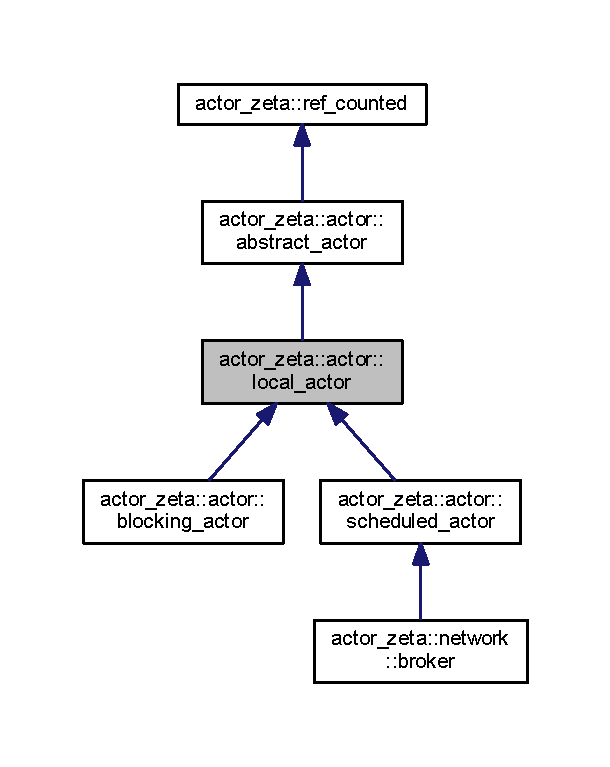
\includegraphics[width=293pt]{classactor__zeta_1_1actor_1_1local__actor__inherit__graph}
\end{center}
\end{figure}


Collaboration diagram for actor\+\_\+zeta\+:\+:actor\+:\+:local\+\_\+actor\+:\nopagebreak
\begin{figure}[H]
\begin{center}
\leavevmode
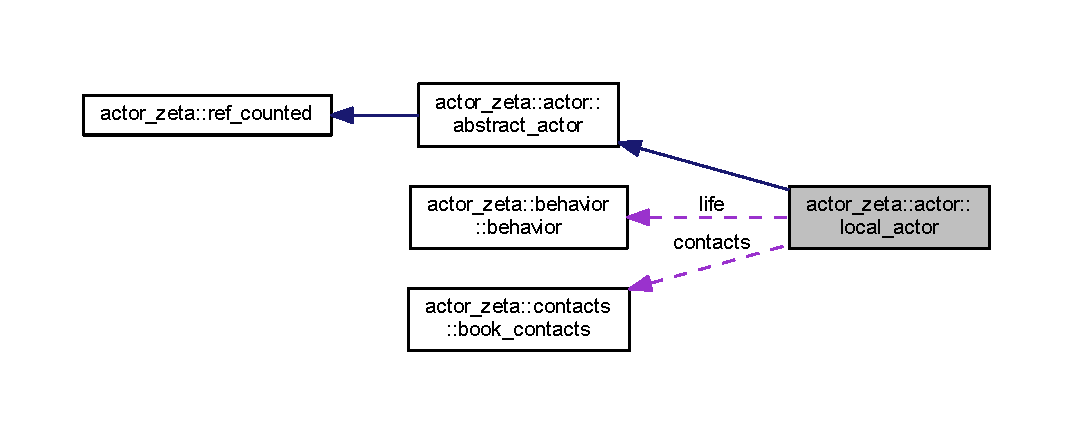
\includegraphics[width=350pt]{classactor__zeta_1_1actor_1_1local__actor__coll__graph}
\end{center}
\end{figure}
\subsection*{Public Types}
\begin{DoxyCompactItemize}
\item 
using \hyperlink{classactor__zeta_1_1actor_1_1local__actor_aacff3ec6e7196584dd640b8d57fa020e}{mailbox\+\_\+type} = \hyperlink{classactor__zeta_1_1messaging_1_1blocking__mail__queue}{messaging\+::blocking\+\_\+mail\+\_\+queue}$<$ \hyperlink{classactor__zeta_1_1messaging_1_1message}{messaging\+::message} $>$
\end{DoxyCompactItemize}
\subsection*{Public Member Functions}
\begin{DoxyCompactItemize}
\item 
virtual void \hyperlink{classactor__zeta_1_1actor_1_1local__actor_acfba412b813aee3250c589bee232f3cd}{launch} (\hyperlink{structactor__zeta_1_1executor_1_1execution__device}{executor\+::execution\+\_\+device} $\ast$, bool)=0
\item 
virtual \hyperlink{classactor__zeta_1_1actor_1_1local__actor_adb1c7cd995fef7b2c3199fa07df6dfca}{$\sim$local\+\_\+actor} ()
\end{DoxyCompactItemize}
\subsection*{Protected Member Functions}
\begin{DoxyCompactItemize}
\item 
void \hyperlink{classactor__zeta_1_1actor_1_1local__actor_a10630eb4ca5d3ef6722743422d6f8d67}{device} (\hyperlink{structactor__zeta_1_1executor_1_1execution__device}{executor\+::execution\+\_\+device} $\ast$e)
\item 
\hyperlink{structactor__zeta_1_1executor_1_1execution__device}{executor\+::execution\+\_\+device} $\ast$ \hyperlink{classactor__zeta_1_1actor_1_1local__actor_ab02f8bbd99a78b15564321336d9e9b59}{device} () const
\item 
void \hyperlink{classactor__zeta_1_1actor_1_1local__actor_a2a64a1b7c7d88cc1bb3b530edea07322}{attach} (\hyperlink{classactor__zeta_1_1behavior_1_1abstract__action}{behavior\+::abstract\+\_\+action} $\ast$)
\item 
\hyperlink{classactor__zeta_1_1actor_1_1local__actor_a10847f855f54d1dbc6f946c75b024cc7}{local\+\_\+actor} (\hyperlink{classactor__zeta_1_1environment_1_1environment}{environment\+::environment} $\ast$, const std\+::string \&)
\item 
virtual void \hyperlink{classactor__zeta_1_1actor_1_1local__actor_ab540625b83fa06318a2ae41dcca4ca16}{initialize} ()
\item 
\hyperlink{classactor__zeta_1_1messaging_1_1message}{messaging\+::message} $\ast$ \hyperlink{classactor__zeta_1_1actor_1_1local__actor_ab149db7088e5c9465c6ded44e47b720f}{next\+\_\+message} ()
\item 
bool \hyperlink{classactor__zeta_1_1actor_1_1local__actor_a48509fa451ade61c97fe65c895639548}{has\+\_\+next\+\_\+message} ()
\item 
\hyperlink{classactor__zeta_1_1actor_1_1local__actor_aacff3ec6e7196584dd640b8d57fa020e}{mailbox\+\_\+type} \& \hyperlink{classactor__zeta_1_1actor_1_1local__actor_afaa5f7042296f91cd741369df0e6585a}{mailbox} ()
\item 
bool \hyperlink{classactor__zeta_1_1actor_1_1local__actor_ae736971463581933ea4daa4958f3cd80}{push\+\_\+to\+\_\+cache} (\hyperlink{classactor__zeta_1_1messaging_1_1message}{messaging\+::message} $\ast$)
\item 
\hyperlink{classactor__zeta_1_1messaging_1_1message}{messaging\+::message} $\ast$ \hyperlink{classactor__zeta_1_1actor_1_1local__actor_a8e8dd70bea2c17895e8aca704e68806a}{pop\+\_\+to\+\_\+cache} ()
\end{DoxyCompactItemize}
\subsection*{Protected Attributes}
\begin{DoxyCompactItemize}
\item 
\hyperlink{classactor__zeta_1_1contacts_1_1book__contacts}{contacts\+::book\+\_\+contacts} \hyperlink{classactor__zeta_1_1actor_1_1local__actor_a4fda781631b136f3ed0adcea9fa69cc4}{contacts}
\item 
\hyperlink{classactor__zeta_1_1behavior_1_1behavior}{behavior\+::behavior} \hyperlink{classactor__zeta_1_1actor_1_1local__actor_a301dcbe374e76903da9cb44c368ac587}{life}
\end{DoxyCompactItemize}


\subsection{Detailed Description}
Class for location dependant type actor. 

\subsection{Member Typedef Documentation}
\mbox{\Hypertarget{classactor__zeta_1_1actor_1_1local__actor_aacff3ec6e7196584dd640b8d57fa020e}\label{classactor__zeta_1_1actor_1_1local__actor_aacff3ec6e7196584dd640b8d57fa020e}} 
\index{actor\+\_\+zeta\+::actor\+::local\+\_\+actor@{actor\+\_\+zeta\+::actor\+::local\+\_\+actor}!mailbox\+\_\+type@{mailbox\+\_\+type}}
\index{mailbox\+\_\+type@{mailbox\+\_\+type}!actor\+\_\+zeta\+::actor\+::local\+\_\+actor@{actor\+\_\+zeta\+::actor\+::local\+\_\+actor}}
\subsubsection{\texorpdfstring{mailbox\+\_\+type}{mailbox\_type}}
{\footnotesize\ttfamily using \hyperlink{classactor__zeta_1_1actor_1_1local__actor_aacff3ec6e7196584dd640b8d57fa020e}{actor\+\_\+zeta\+::actor\+::local\+\_\+actor\+::mailbox\+\_\+type} =  \hyperlink{classactor__zeta_1_1messaging_1_1blocking__mail__queue}{messaging\+::blocking\+\_\+mail\+\_\+queue}$<$\hyperlink{classactor__zeta_1_1messaging_1_1message}{messaging\+::message}$>$}



\subsection{Constructor \& Destructor Documentation}
\mbox{\Hypertarget{classactor__zeta_1_1actor_1_1local__actor_adb1c7cd995fef7b2c3199fa07df6dfca}\label{classactor__zeta_1_1actor_1_1local__actor_adb1c7cd995fef7b2c3199fa07df6dfca}} 
\index{actor\+\_\+zeta\+::actor\+::local\+\_\+actor@{actor\+\_\+zeta\+::actor\+::local\+\_\+actor}!````~local\+\_\+actor@{$\sim$local\+\_\+actor}}
\index{````~local\+\_\+actor@{$\sim$local\+\_\+actor}!actor\+\_\+zeta\+::actor\+::local\+\_\+actor@{actor\+\_\+zeta\+::actor\+::local\+\_\+actor}}
\subsubsection{\texorpdfstring{$\sim$local\+\_\+actor()}{~local\_actor()}}
{\footnotesize\ttfamily actor\+\_\+zeta\+::actor\+::local\+\_\+actor\+::$\sim$local\+\_\+actor (\begin{DoxyParamCaption}{ }\end{DoxyParamCaption})\hspace{0.3cm}{\ttfamily [virtual]}}

\mbox{\Hypertarget{classactor__zeta_1_1actor_1_1local__actor_a10847f855f54d1dbc6f946c75b024cc7}\label{classactor__zeta_1_1actor_1_1local__actor_a10847f855f54d1dbc6f946c75b024cc7}} 
\index{actor\+\_\+zeta\+::actor\+::local\+\_\+actor@{actor\+\_\+zeta\+::actor\+::local\+\_\+actor}!local\+\_\+actor@{local\+\_\+actor}}
\index{local\+\_\+actor@{local\+\_\+actor}!actor\+\_\+zeta\+::actor\+::local\+\_\+actor@{actor\+\_\+zeta\+::actor\+::local\+\_\+actor}}
\subsubsection{\texorpdfstring{local\+\_\+actor()}{local\_actor()}}
{\footnotesize\ttfamily actor\+\_\+zeta\+::actor\+::local\+\_\+actor\+::local\+\_\+actor (\begin{DoxyParamCaption}\item[{\hyperlink{classactor__zeta_1_1environment_1_1environment}{environment\+::environment} $\ast$}]{env,  }\item[{const std\+::string \&}]{type }\end{DoxyParamCaption})\hspace{0.3cm}{\ttfamily [protected]}}



\subsection{Member Function Documentation}
\mbox{\Hypertarget{classactor__zeta_1_1actor_1_1local__actor_a2a64a1b7c7d88cc1bb3b530edea07322}\label{classactor__zeta_1_1actor_1_1local__actor_a2a64a1b7c7d88cc1bb3b530edea07322}} 
\index{actor\+\_\+zeta\+::actor\+::local\+\_\+actor@{actor\+\_\+zeta\+::actor\+::local\+\_\+actor}!attach@{attach}}
\index{attach@{attach}!actor\+\_\+zeta\+::actor\+::local\+\_\+actor@{actor\+\_\+zeta\+::actor\+::local\+\_\+actor}}
\subsubsection{\texorpdfstring{attach()}{attach()}}
{\footnotesize\ttfamily void actor\+\_\+zeta\+::actor\+::local\+\_\+actor\+::attach (\begin{DoxyParamCaption}\item[{\hyperlink{classactor__zeta_1_1behavior_1_1abstract__action}{behavior\+::abstract\+\_\+action} $\ast$}]{ptr\+\_\+aa }\end{DoxyParamCaption})\hspace{0.3cm}{\ttfamily [protected]}}

\mbox{\Hypertarget{classactor__zeta_1_1actor_1_1local__actor_a10630eb4ca5d3ef6722743422d6f8d67}\label{classactor__zeta_1_1actor_1_1local__actor_a10630eb4ca5d3ef6722743422d6f8d67}} 
\index{actor\+\_\+zeta\+::actor\+::local\+\_\+actor@{actor\+\_\+zeta\+::actor\+::local\+\_\+actor}!device@{device}}
\index{device@{device}!actor\+\_\+zeta\+::actor\+::local\+\_\+actor@{actor\+\_\+zeta\+::actor\+::local\+\_\+actor}}
\subsubsection{\texorpdfstring{device()}{device()}\hspace{0.1cm}{\footnotesize\ttfamily [1/2]}}
{\footnotesize\ttfamily void actor\+\_\+zeta\+::actor\+::local\+\_\+actor\+::device (\begin{DoxyParamCaption}\item[{\hyperlink{structactor__zeta_1_1executor_1_1execution__device}{executor\+::execution\+\_\+device} $\ast$}]{e }\end{DoxyParamCaption})\hspace{0.3cm}{\ttfamily [inline]}, {\ttfamily [protected]}}

\mbox{\Hypertarget{classactor__zeta_1_1actor_1_1local__actor_ab02f8bbd99a78b15564321336d9e9b59}\label{classactor__zeta_1_1actor_1_1local__actor_ab02f8bbd99a78b15564321336d9e9b59}} 
\index{actor\+\_\+zeta\+::actor\+::local\+\_\+actor@{actor\+\_\+zeta\+::actor\+::local\+\_\+actor}!device@{device}}
\index{device@{device}!actor\+\_\+zeta\+::actor\+::local\+\_\+actor@{actor\+\_\+zeta\+::actor\+::local\+\_\+actor}}
\subsubsection{\texorpdfstring{device()}{device()}\hspace{0.1cm}{\footnotesize\ttfamily [2/2]}}
{\footnotesize\ttfamily \hyperlink{structactor__zeta_1_1executor_1_1execution__device}{executor\+::execution\+\_\+device}$\ast$ actor\+\_\+zeta\+::actor\+::local\+\_\+actor\+::device (\begin{DoxyParamCaption}{ }\end{DoxyParamCaption}) const\hspace{0.3cm}{\ttfamily [inline]}, {\ttfamily [protected]}}

\mbox{\Hypertarget{classactor__zeta_1_1actor_1_1local__actor_a48509fa451ade61c97fe65c895639548}\label{classactor__zeta_1_1actor_1_1local__actor_a48509fa451ade61c97fe65c895639548}} 
\index{actor\+\_\+zeta\+::actor\+::local\+\_\+actor@{actor\+\_\+zeta\+::actor\+::local\+\_\+actor}!has\+\_\+next\+\_\+message@{has\+\_\+next\+\_\+message}}
\index{has\+\_\+next\+\_\+message@{has\+\_\+next\+\_\+message}!actor\+\_\+zeta\+::actor\+::local\+\_\+actor@{actor\+\_\+zeta\+::actor\+::local\+\_\+actor}}
\subsubsection{\texorpdfstring{has\+\_\+next\+\_\+message()}{has\_next\_message()}}
{\footnotesize\ttfamily bool actor\+\_\+zeta\+::actor\+::local\+\_\+actor\+::has\+\_\+next\+\_\+message (\begin{DoxyParamCaption}{ }\end{DoxyParamCaption})\hspace{0.3cm}{\ttfamily [protected]}}

\mbox{\Hypertarget{classactor__zeta_1_1actor_1_1local__actor_ab540625b83fa06318a2ae41dcca4ca16}\label{classactor__zeta_1_1actor_1_1local__actor_ab540625b83fa06318a2ae41dcca4ca16}} 
\index{actor\+\_\+zeta\+::actor\+::local\+\_\+actor@{actor\+\_\+zeta\+::actor\+::local\+\_\+actor}!initialize@{initialize}}
\index{initialize@{initialize}!actor\+\_\+zeta\+::actor\+::local\+\_\+actor@{actor\+\_\+zeta\+::actor\+::local\+\_\+actor}}
\subsubsection{\texorpdfstring{initialize()}{initialize()}}
{\footnotesize\ttfamily void actor\+\_\+zeta\+::actor\+::local\+\_\+actor\+::initialize (\begin{DoxyParamCaption}{ }\end{DoxyParamCaption})\hspace{0.3cm}{\ttfamily [protected]}, {\ttfamily [virtual]}}



Reimplemented in \hyperlink{classactor__zeta_1_1network_1_1broker_a5e63848370208ff7e670ec08ea7b3cf9}{actor\+\_\+zeta\+::network\+::broker}.

\mbox{\Hypertarget{classactor__zeta_1_1actor_1_1local__actor_acfba412b813aee3250c589bee232f3cd}\label{classactor__zeta_1_1actor_1_1local__actor_acfba412b813aee3250c589bee232f3cd}} 
\index{actor\+\_\+zeta\+::actor\+::local\+\_\+actor@{actor\+\_\+zeta\+::actor\+::local\+\_\+actor}!launch@{launch}}
\index{launch@{launch}!actor\+\_\+zeta\+::actor\+::local\+\_\+actor@{actor\+\_\+zeta\+::actor\+::local\+\_\+actor}}
\subsubsection{\texorpdfstring{launch()}{launch()}}
{\footnotesize\ttfamily virtual void actor\+\_\+zeta\+::actor\+::local\+\_\+actor\+::launch (\begin{DoxyParamCaption}\item[{\hyperlink{structactor__zeta_1_1executor_1_1execution__device}{executor\+::execution\+\_\+device} $\ast$}]{,  }\item[{bool}]{ }\end{DoxyParamCaption})\hspace{0.3cm}{\ttfamily [pure virtual]}}



Implemented in \hyperlink{classactor__zeta_1_1actor_1_1scheduled__actor_a15dcbee3ab1540c7ed675846cbf10726}{actor\+\_\+zeta\+::actor\+::scheduled\+\_\+actor}, and \hyperlink{classactor__zeta_1_1actor_1_1blocking__actor_a7988829bb7d264b3f226f8c5d4156cb1}{actor\+\_\+zeta\+::actor\+::blocking\+\_\+actor}.

\mbox{\Hypertarget{classactor__zeta_1_1actor_1_1local__actor_afaa5f7042296f91cd741369df0e6585a}\label{classactor__zeta_1_1actor_1_1local__actor_afaa5f7042296f91cd741369df0e6585a}} 
\index{actor\+\_\+zeta\+::actor\+::local\+\_\+actor@{actor\+\_\+zeta\+::actor\+::local\+\_\+actor}!mailbox@{mailbox}}
\index{mailbox@{mailbox}!actor\+\_\+zeta\+::actor\+::local\+\_\+actor@{actor\+\_\+zeta\+::actor\+::local\+\_\+actor}}
\subsubsection{\texorpdfstring{mailbox()}{mailbox()}}
{\footnotesize\ttfamily \hyperlink{classactor__zeta_1_1actor_1_1local__actor_aacff3ec6e7196584dd640b8d57fa020e}{mailbox\+\_\+type}\& actor\+\_\+zeta\+::actor\+::local\+\_\+actor\+::mailbox (\begin{DoxyParamCaption}{ }\end{DoxyParamCaption})\hspace{0.3cm}{\ttfamily [inline]}, {\ttfamily [protected]}}

\mbox{\Hypertarget{classactor__zeta_1_1actor_1_1local__actor_ab149db7088e5c9465c6ded44e47b720f}\label{classactor__zeta_1_1actor_1_1local__actor_ab149db7088e5c9465c6ded44e47b720f}} 
\index{actor\+\_\+zeta\+::actor\+::local\+\_\+actor@{actor\+\_\+zeta\+::actor\+::local\+\_\+actor}!next\+\_\+message@{next\+\_\+message}}
\index{next\+\_\+message@{next\+\_\+message}!actor\+\_\+zeta\+::actor\+::local\+\_\+actor@{actor\+\_\+zeta\+::actor\+::local\+\_\+actor}}
\subsubsection{\texorpdfstring{next\+\_\+message()}{next\_message()}}
{\footnotesize\ttfamily \hyperlink{classactor__zeta_1_1messaging_1_1message}{messaging\+::message} $\ast$ actor\+\_\+zeta\+::actor\+::local\+\_\+actor\+::next\+\_\+message (\begin{DoxyParamCaption}{ }\end{DoxyParamCaption})\hspace{0.3cm}{\ttfamily [protected]}}

\mbox{\Hypertarget{classactor__zeta_1_1actor_1_1local__actor_a8e8dd70bea2c17895e8aca704e68806a}\label{classactor__zeta_1_1actor_1_1local__actor_a8e8dd70bea2c17895e8aca704e68806a}} 
\index{actor\+\_\+zeta\+::actor\+::local\+\_\+actor@{actor\+\_\+zeta\+::actor\+::local\+\_\+actor}!pop\+\_\+to\+\_\+cache@{pop\+\_\+to\+\_\+cache}}
\index{pop\+\_\+to\+\_\+cache@{pop\+\_\+to\+\_\+cache}!actor\+\_\+zeta\+::actor\+::local\+\_\+actor@{actor\+\_\+zeta\+::actor\+::local\+\_\+actor}}
\subsubsection{\texorpdfstring{pop\+\_\+to\+\_\+cache()}{pop\_to\_cache()}}
{\footnotesize\ttfamily \hyperlink{classactor__zeta_1_1messaging_1_1message}{messaging\+::message} $\ast$ actor\+\_\+zeta\+::actor\+::local\+\_\+actor\+::pop\+\_\+to\+\_\+cache (\begin{DoxyParamCaption}{ }\end{DoxyParamCaption})\hspace{0.3cm}{\ttfamily [protected]}}

\mbox{\Hypertarget{classactor__zeta_1_1actor_1_1local__actor_ae736971463581933ea4daa4958f3cd80}\label{classactor__zeta_1_1actor_1_1local__actor_ae736971463581933ea4daa4958f3cd80}} 
\index{actor\+\_\+zeta\+::actor\+::local\+\_\+actor@{actor\+\_\+zeta\+::actor\+::local\+\_\+actor}!push\+\_\+to\+\_\+cache@{push\+\_\+to\+\_\+cache}}
\index{push\+\_\+to\+\_\+cache@{push\+\_\+to\+\_\+cache}!actor\+\_\+zeta\+::actor\+::local\+\_\+actor@{actor\+\_\+zeta\+::actor\+::local\+\_\+actor}}
\subsubsection{\texorpdfstring{push\+\_\+to\+\_\+cache()}{push\_to\_cache()}}
{\footnotesize\ttfamily bool actor\+\_\+zeta\+::actor\+::local\+\_\+actor\+::push\+\_\+to\+\_\+cache (\begin{DoxyParamCaption}\item[{\hyperlink{classactor__zeta_1_1messaging_1_1message}{messaging\+::message} $\ast$}]{msg\+\_\+ptr }\end{DoxyParamCaption})\hspace{0.3cm}{\ttfamily [protected]}}



\subsection{Member Data Documentation}
\mbox{\Hypertarget{classactor__zeta_1_1actor_1_1local__actor_a4fda781631b136f3ed0adcea9fa69cc4}\label{classactor__zeta_1_1actor_1_1local__actor_a4fda781631b136f3ed0adcea9fa69cc4}} 
\index{actor\+\_\+zeta\+::actor\+::local\+\_\+actor@{actor\+\_\+zeta\+::actor\+::local\+\_\+actor}!contacts@{contacts}}
\index{contacts@{contacts}!actor\+\_\+zeta\+::actor\+::local\+\_\+actor@{actor\+\_\+zeta\+::actor\+::local\+\_\+actor}}
\subsubsection{\texorpdfstring{contacts}{contacts}}
{\footnotesize\ttfamily \hyperlink{classactor__zeta_1_1contacts_1_1book__contacts}{contacts\+::book\+\_\+contacts} actor\+\_\+zeta\+::actor\+::local\+\_\+actor\+::contacts\hspace{0.3cm}{\ttfamily [protected]}}

\mbox{\Hypertarget{classactor__zeta_1_1actor_1_1local__actor_a301dcbe374e76903da9cb44c368ac587}\label{classactor__zeta_1_1actor_1_1local__actor_a301dcbe374e76903da9cb44c368ac587}} 
\index{actor\+\_\+zeta\+::actor\+::local\+\_\+actor@{actor\+\_\+zeta\+::actor\+::local\+\_\+actor}!life@{life}}
\index{life@{life}!actor\+\_\+zeta\+::actor\+::local\+\_\+actor@{actor\+\_\+zeta\+::actor\+::local\+\_\+actor}}
\subsubsection{\texorpdfstring{life}{life}}
{\footnotesize\ttfamily \hyperlink{classactor__zeta_1_1behavior_1_1behavior}{behavior\+::behavior} actor\+\_\+zeta\+::actor\+::local\+\_\+actor\+::life\hspace{0.3cm}{\ttfamily [protected]}}



The documentation for this class was generated from the following files\+:\begin{DoxyCompactItemize}
\item 
\hyperlink{local__actor_8hpp}{local\+\_\+actor.\+hpp}\item 
\hyperlink{local__actor_8cpp}{local\+\_\+actor.\+cpp}\end{DoxyCompactItemize}

\hypertarget{classactor__zeta_1_1messaging_1_1message}{}\section{actor\+\_\+zeta\+:\+:messaging\+:\+:message Class Reference}
\label{classactor__zeta_1_1messaging_1_1message}\index{actor\+\_\+zeta\+::messaging\+::message@{actor\+\_\+zeta\+::messaging\+::message}}


Class to represent messages.  




{\ttfamily \#include $<$message.\+hpp$>$}

\subsection*{Public Member Functions}
\begin{DoxyCompactItemize}
\item 
\hyperlink{classactor__zeta_1_1messaging_1_1message_ad2d5ed4012814ff6e374eab24bb6079d}{message} ()=delete
\item 
\hyperlink{classactor__zeta_1_1messaging_1_1message_aedfd2ae19160098b4b3616bf121854b3}{message} (const \hyperlink{classactor__zeta_1_1messaging_1_1message}{message} \&)=delete
\item 
\hyperlink{classactor__zeta_1_1messaging_1_1message}{message} \& \hyperlink{classactor__zeta_1_1messaging_1_1message_a3829befdc05243773eb02668c830a25a}{operator=} (const \hyperlink{classactor__zeta_1_1messaging_1_1message}{message} \&)=delete
\item 
\hyperlink{classactor__zeta_1_1messaging_1_1message_a55927d9741c28bd3bc003a4daf4e793d}{message} (\hyperlink{classactor__zeta_1_1messaging_1_1message}{message} \&\&)=default
\item 
\hyperlink{classactor__zeta_1_1messaging_1_1message}{message} \& \hyperlink{classactor__zeta_1_1messaging_1_1message_a3cfe617e41808c075afa2dbd32ea9ef4}{operator=} (\hyperlink{classactor__zeta_1_1messaging_1_1message}{message} \&\&)=default
\item 
\hyperlink{classactor__zeta_1_1messaging_1_1message_a984fb448900c694424545be2f44be846}{$\sim$message} ()=default
\item 
{\footnotesize template$<$std\+::size\+\_\+t N, typename T $>$ }\\\hyperlink{classactor__zeta_1_1messaging_1_1message_a477f95504ed3d8ea6097dfaa1b053ade}{message} (const char(\&a\+Str)\mbox{[}N\mbox{]}, const T \&t)
\item 
{\footnotesize template$<$std\+::size\+\_\+t N, typename T $>$ }\\\hyperlink{classactor__zeta_1_1messaging_1_1message_a00398df5618923c839797568ce955d69}{message} (const char(\&a\+Str)\mbox{[}N\mbox{]}, const T \&t, \hyperlink{classactor__zeta_1_1actor_1_1actor__address}{actor\+::actor\+\_\+address} aa)
\item 
{\footnotesize template$<$std\+::size\+\_\+t N, typename T $>$ }\\\hyperlink{classactor__zeta_1_1messaging_1_1message_a0c8be6b9a9cba1a7a2142f031cdcbfbe}{message} (const char(\&a\+Str)\mbox{[}N\mbox{]}, const T \&t, \hyperlink{namespaceactor__zeta_1_1messaging_a1b4c4b3ab625eb033c15da4fbe9c4a89}{message\+\_\+priority} p)
\item 
{\footnotesize template$<$std\+::size\+\_\+t N, typename T $>$ }\\\hyperlink{classactor__zeta_1_1messaging_1_1message_abee9c14df4e91017a6f377d916409854}{message} (const char(\&a\+Str)\mbox{[}N\mbox{]}, const T \&t, \hyperlink{namespaceactor__zeta_1_1messaging_a1b4c4b3ab625eb033c15da4fbe9c4a89}{message\+\_\+priority} p, \hyperlink{classactor__zeta_1_1actor_1_1actor__address}{actor\+::actor\+\_\+address} aa)
\item 
{\footnotesize template$<$typename T $>$ }\\\hyperlink{classactor__zeta_1_1messaging_1_1message_a8caea1df1350631fa5c803e3ac368c6d}{message} (const char $\ast$str, std\+::size\+\_\+t len, const T \&t)
\item 
{\footnotesize template$<$typename T $>$ }\\\hyperlink{classactor__zeta_1_1messaging_1_1message_a1e2810d89cc8f75aa451057fe7252e07}{message} (const char $\ast$str, std\+::size\+\_\+t len, const T \&t, \hyperlink{classactor__zeta_1_1actor_1_1actor__address}{actor\+::actor\+\_\+address} aa)
\item 
{\footnotesize template$<$typename T $>$ }\\\hyperlink{classactor__zeta_1_1messaging_1_1message_a0428ac91ee6cdf4b4a99a2f7c262cc0c}{message} (const char $\ast$str, std\+::size\+\_\+t len, const T \&t, \hyperlink{namespaceactor__zeta_1_1messaging_a1b4c4b3ab625eb033c15da4fbe9c4a89}{message\+\_\+priority} p)
\item 
{\footnotesize template$<$typename T $>$ }\\\hyperlink{classactor__zeta_1_1messaging_1_1message_a145a2691247f874ab57ff964512631c1}{message} (const char $\ast$str, std\+::size\+\_\+t len, const T \&t, \hyperlink{namespaceactor__zeta_1_1messaging_a1b4c4b3ab625eb033c15da4fbe9c4a89}{message\+\_\+priority} p, \hyperlink{classactor__zeta_1_1actor_1_1actor__address}{actor\+::actor\+\_\+address} aa)
\item 
\hyperlink{namespaceactor__zeta_1_1messaging_a1b4c4b3ab625eb033c15da4fbe9c4a89}{message\+\_\+priority} \hyperlink{classactor__zeta_1_1messaging_1_1message_af5f7ce0e94bfae703f84c358cefe80d5}{priority} () const
\item 
auto \hyperlink{classactor__zeta_1_1messaging_1_1message_a5d44fe019c0e2451ed0add86e7403226}{type} () const noexcept -\/$>$ const \hyperlink{classactor__zeta_1_1behavior_1_1type__action}{behavior\+::type\+\_\+action} \&
\item 
\hyperlink{classactor__zeta_1_1actor_1_1actor__address}{actor\+::actor\+\_\+address} \hyperlink{classactor__zeta_1_1messaging_1_1message_af1a8a856212d754964b9ef80d6f70e9e}{return\+\_\+address} () const
\item 
bool \hyperlink{classactor__zeta_1_1messaging_1_1message_a8384e47a23f78c49075edd57797d3791}{is\+\_\+callback} () const
\item 
{\footnotesize template$<$typename T $>$ }\\auto \hyperlink{classactor__zeta_1_1messaging_1_1message_a3e6147856c28d39c3786f1ea8a64213a}{get} () -\/$>$ T
\item 
auto \hyperlink{classactor__zeta_1_1messaging_1_1message_a5206bd7a0def3cb864a3468cee2d37e2}{clone} () const -\/$>$ \hyperlink{classactor__zeta_1_1messaging_1_1message}{message} $\ast$
\end{DoxyCompactItemize}


\subsection{Detailed Description}
Class to represent messages. 

\subsection{Constructor \& Destructor Documentation}
\mbox{\Hypertarget{classactor__zeta_1_1messaging_1_1message_ad2d5ed4012814ff6e374eab24bb6079d}\label{classactor__zeta_1_1messaging_1_1message_ad2d5ed4012814ff6e374eab24bb6079d}} 
\index{actor\+\_\+zeta\+::messaging\+::message@{actor\+\_\+zeta\+::messaging\+::message}!message@{message}}
\index{message@{message}!actor\+\_\+zeta\+::messaging\+::message@{actor\+\_\+zeta\+::messaging\+::message}}
\subsubsection{\texorpdfstring{message()}{message()}\hspace{0.1cm}{\footnotesize\ttfamily [1/11]}}
{\footnotesize\ttfamily actor\+\_\+zeta\+::messaging\+::message\+::message (\begin{DoxyParamCaption}{ }\end{DoxyParamCaption})\hspace{0.3cm}{\ttfamily [delete]}}

\mbox{\Hypertarget{classactor__zeta_1_1messaging_1_1message_aedfd2ae19160098b4b3616bf121854b3}\label{classactor__zeta_1_1messaging_1_1message_aedfd2ae19160098b4b3616bf121854b3}} 
\index{actor\+\_\+zeta\+::messaging\+::message@{actor\+\_\+zeta\+::messaging\+::message}!message@{message}}
\index{message@{message}!actor\+\_\+zeta\+::messaging\+::message@{actor\+\_\+zeta\+::messaging\+::message}}
\subsubsection{\texorpdfstring{message()}{message()}\hspace{0.1cm}{\footnotesize\ttfamily [2/11]}}
{\footnotesize\ttfamily actor\+\_\+zeta\+::messaging\+::message\+::message (\begin{DoxyParamCaption}\item[{const \hyperlink{classactor__zeta_1_1messaging_1_1message}{message} \&}]{ }\end{DoxyParamCaption})\hspace{0.3cm}{\ttfamily [delete]}}

\mbox{\Hypertarget{classactor__zeta_1_1messaging_1_1message_a55927d9741c28bd3bc003a4daf4e793d}\label{classactor__zeta_1_1messaging_1_1message_a55927d9741c28bd3bc003a4daf4e793d}} 
\index{actor\+\_\+zeta\+::messaging\+::message@{actor\+\_\+zeta\+::messaging\+::message}!message@{message}}
\index{message@{message}!actor\+\_\+zeta\+::messaging\+::message@{actor\+\_\+zeta\+::messaging\+::message}}
\subsubsection{\texorpdfstring{message()}{message()}\hspace{0.1cm}{\footnotesize\ttfamily [3/11]}}
{\footnotesize\ttfamily actor\+\_\+zeta\+::messaging\+::message\+::message (\begin{DoxyParamCaption}\item[{\hyperlink{classactor__zeta_1_1messaging_1_1message}{message} \&\&}]{ }\end{DoxyParamCaption})\hspace{0.3cm}{\ttfamily [default]}}

\mbox{\Hypertarget{classactor__zeta_1_1messaging_1_1message_a984fb448900c694424545be2f44be846}\label{classactor__zeta_1_1messaging_1_1message_a984fb448900c694424545be2f44be846}} 
\index{actor\+\_\+zeta\+::messaging\+::message@{actor\+\_\+zeta\+::messaging\+::message}!````~message@{$\sim$message}}
\index{````~message@{$\sim$message}!actor\+\_\+zeta\+::messaging\+::message@{actor\+\_\+zeta\+::messaging\+::message}}
\subsubsection{\texorpdfstring{$\sim$message()}{~message()}}
{\footnotesize\ttfamily actor\+\_\+zeta\+::messaging\+::message\+::$\sim$message (\begin{DoxyParamCaption}{ }\end{DoxyParamCaption})\hspace{0.3cm}{\ttfamily [default]}}

\mbox{\Hypertarget{classactor__zeta_1_1messaging_1_1message_a477f95504ed3d8ea6097dfaa1b053ade}\label{classactor__zeta_1_1messaging_1_1message_a477f95504ed3d8ea6097dfaa1b053ade}} 
\index{actor\+\_\+zeta\+::messaging\+::message@{actor\+\_\+zeta\+::messaging\+::message}!message@{message}}
\index{message@{message}!actor\+\_\+zeta\+::messaging\+::message@{actor\+\_\+zeta\+::messaging\+::message}}
\subsubsection{\texorpdfstring{message()}{message()}\hspace{0.1cm}{\footnotesize\ttfamily [4/11]}}
{\footnotesize\ttfamily template$<$std\+::size\+\_\+t N, typename T $>$ \\
actor\+\_\+zeta\+::messaging\+::message\+::message (\begin{DoxyParamCaption}\item[{const char(\&)}]{a\+Str\mbox{[}\+N\mbox{]},  }\item[{const T \&}]{t }\end{DoxyParamCaption})\hspace{0.3cm}{\ttfamily [inline]}}

\mbox{\Hypertarget{classactor__zeta_1_1messaging_1_1message_a00398df5618923c839797568ce955d69}\label{classactor__zeta_1_1messaging_1_1message_a00398df5618923c839797568ce955d69}} 
\index{actor\+\_\+zeta\+::messaging\+::message@{actor\+\_\+zeta\+::messaging\+::message}!message@{message}}
\index{message@{message}!actor\+\_\+zeta\+::messaging\+::message@{actor\+\_\+zeta\+::messaging\+::message}}
\subsubsection{\texorpdfstring{message()}{message()}\hspace{0.1cm}{\footnotesize\ttfamily [5/11]}}
{\footnotesize\ttfamily template$<$std\+::size\+\_\+t N, typename T $>$ \\
actor\+\_\+zeta\+::messaging\+::message\+::message (\begin{DoxyParamCaption}\item[{const char(\&)}]{a\+Str\mbox{[}\+N\mbox{]},  }\item[{const T \&}]{t,  }\item[{\hyperlink{classactor__zeta_1_1actor_1_1actor__address}{actor\+::actor\+\_\+address}}]{aa }\end{DoxyParamCaption})\hspace{0.3cm}{\ttfamily [inline]}}

\mbox{\Hypertarget{classactor__zeta_1_1messaging_1_1message_a0c8be6b9a9cba1a7a2142f031cdcbfbe}\label{classactor__zeta_1_1messaging_1_1message_a0c8be6b9a9cba1a7a2142f031cdcbfbe}} 
\index{actor\+\_\+zeta\+::messaging\+::message@{actor\+\_\+zeta\+::messaging\+::message}!message@{message}}
\index{message@{message}!actor\+\_\+zeta\+::messaging\+::message@{actor\+\_\+zeta\+::messaging\+::message}}
\subsubsection{\texorpdfstring{message()}{message()}\hspace{0.1cm}{\footnotesize\ttfamily [6/11]}}
{\footnotesize\ttfamily template$<$std\+::size\+\_\+t N, typename T $>$ \\
actor\+\_\+zeta\+::messaging\+::message\+::message (\begin{DoxyParamCaption}\item[{const char(\&)}]{a\+Str\mbox{[}\+N\mbox{]},  }\item[{const T \&}]{t,  }\item[{\hyperlink{namespaceactor__zeta_1_1messaging_a1b4c4b3ab625eb033c15da4fbe9c4a89}{message\+\_\+priority}}]{p }\end{DoxyParamCaption})\hspace{0.3cm}{\ttfamily [inline]}}

\mbox{\Hypertarget{classactor__zeta_1_1messaging_1_1message_abee9c14df4e91017a6f377d916409854}\label{classactor__zeta_1_1messaging_1_1message_abee9c14df4e91017a6f377d916409854}} 
\index{actor\+\_\+zeta\+::messaging\+::message@{actor\+\_\+zeta\+::messaging\+::message}!message@{message}}
\index{message@{message}!actor\+\_\+zeta\+::messaging\+::message@{actor\+\_\+zeta\+::messaging\+::message}}
\subsubsection{\texorpdfstring{message()}{message()}\hspace{0.1cm}{\footnotesize\ttfamily [7/11]}}
{\footnotesize\ttfamily template$<$std\+::size\+\_\+t N, typename T $>$ \\
actor\+\_\+zeta\+::messaging\+::message\+::message (\begin{DoxyParamCaption}\item[{const char(\&)}]{a\+Str\mbox{[}\+N\mbox{]},  }\item[{const T \&}]{t,  }\item[{\hyperlink{namespaceactor__zeta_1_1messaging_a1b4c4b3ab625eb033c15da4fbe9c4a89}{message\+\_\+priority}}]{p,  }\item[{\hyperlink{classactor__zeta_1_1actor_1_1actor__address}{actor\+::actor\+\_\+address}}]{aa }\end{DoxyParamCaption})\hspace{0.3cm}{\ttfamily [inline]}}

\mbox{\Hypertarget{classactor__zeta_1_1messaging_1_1message_a8caea1df1350631fa5c803e3ac368c6d}\label{classactor__zeta_1_1messaging_1_1message_a8caea1df1350631fa5c803e3ac368c6d}} 
\index{actor\+\_\+zeta\+::messaging\+::message@{actor\+\_\+zeta\+::messaging\+::message}!message@{message}}
\index{message@{message}!actor\+\_\+zeta\+::messaging\+::message@{actor\+\_\+zeta\+::messaging\+::message}}
\subsubsection{\texorpdfstring{message()}{message()}\hspace{0.1cm}{\footnotesize\ttfamily [8/11]}}
{\footnotesize\ttfamily template$<$typename T $>$ \\
actor\+\_\+zeta\+::messaging\+::message\+::message (\begin{DoxyParamCaption}\item[{const char $\ast$}]{str,  }\item[{std\+::size\+\_\+t}]{len,  }\item[{const T \&}]{t }\end{DoxyParamCaption})\hspace{0.3cm}{\ttfamily [inline]}}

\mbox{\Hypertarget{classactor__zeta_1_1messaging_1_1message_a1e2810d89cc8f75aa451057fe7252e07}\label{classactor__zeta_1_1messaging_1_1message_a1e2810d89cc8f75aa451057fe7252e07}} 
\index{actor\+\_\+zeta\+::messaging\+::message@{actor\+\_\+zeta\+::messaging\+::message}!message@{message}}
\index{message@{message}!actor\+\_\+zeta\+::messaging\+::message@{actor\+\_\+zeta\+::messaging\+::message}}
\subsubsection{\texorpdfstring{message()}{message()}\hspace{0.1cm}{\footnotesize\ttfamily [9/11]}}
{\footnotesize\ttfamily template$<$typename T $>$ \\
actor\+\_\+zeta\+::messaging\+::message\+::message (\begin{DoxyParamCaption}\item[{const char $\ast$}]{str,  }\item[{std\+::size\+\_\+t}]{len,  }\item[{const T \&}]{t,  }\item[{\hyperlink{classactor__zeta_1_1actor_1_1actor__address}{actor\+::actor\+\_\+address}}]{aa }\end{DoxyParamCaption})\hspace{0.3cm}{\ttfamily [inline]}}

\mbox{\Hypertarget{classactor__zeta_1_1messaging_1_1message_a0428ac91ee6cdf4b4a99a2f7c262cc0c}\label{classactor__zeta_1_1messaging_1_1message_a0428ac91ee6cdf4b4a99a2f7c262cc0c}} 
\index{actor\+\_\+zeta\+::messaging\+::message@{actor\+\_\+zeta\+::messaging\+::message}!message@{message}}
\index{message@{message}!actor\+\_\+zeta\+::messaging\+::message@{actor\+\_\+zeta\+::messaging\+::message}}
\subsubsection{\texorpdfstring{message()}{message()}\hspace{0.1cm}{\footnotesize\ttfamily [10/11]}}
{\footnotesize\ttfamily template$<$typename T $>$ \\
actor\+\_\+zeta\+::messaging\+::message\+::message (\begin{DoxyParamCaption}\item[{const char $\ast$}]{str,  }\item[{std\+::size\+\_\+t}]{len,  }\item[{const T \&}]{t,  }\item[{\hyperlink{namespaceactor__zeta_1_1messaging_a1b4c4b3ab625eb033c15da4fbe9c4a89}{message\+\_\+priority}}]{p }\end{DoxyParamCaption})\hspace{0.3cm}{\ttfamily [inline]}}

\mbox{\Hypertarget{classactor__zeta_1_1messaging_1_1message_a145a2691247f874ab57ff964512631c1}\label{classactor__zeta_1_1messaging_1_1message_a145a2691247f874ab57ff964512631c1}} 
\index{actor\+\_\+zeta\+::messaging\+::message@{actor\+\_\+zeta\+::messaging\+::message}!message@{message}}
\index{message@{message}!actor\+\_\+zeta\+::messaging\+::message@{actor\+\_\+zeta\+::messaging\+::message}}
\subsubsection{\texorpdfstring{message()}{message()}\hspace{0.1cm}{\footnotesize\ttfamily [11/11]}}
{\footnotesize\ttfamily template$<$typename T $>$ \\
actor\+\_\+zeta\+::messaging\+::message\+::message (\begin{DoxyParamCaption}\item[{const char $\ast$}]{str,  }\item[{std\+::size\+\_\+t}]{len,  }\item[{const T \&}]{t,  }\item[{\hyperlink{namespaceactor__zeta_1_1messaging_a1b4c4b3ab625eb033c15da4fbe9c4a89}{message\+\_\+priority}}]{p,  }\item[{\hyperlink{classactor__zeta_1_1actor_1_1actor__address}{actor\+::actor\+\_\+address}}]{aa }\end{DoxyParamCaption})\hspace{0.3cm}{\ttfamily [inline]}}



\subsection{Member Function Documentation}
\mbox{\Hypertarget{classactor__zeta_1_1messaging_1_1message_a5206bd7a0def3cb864a3468cee2d37e2}\label{classactor__zeta_1_1messaging_1_1message_a5206bd7a0def3cb864a3468cee2d37e2}} 
\index{actor\+\_\+zeta\+::messaging\+::message@{actor\+\_\+zeta\+::messaging\+::message}!clone@{clone}}
\index{clone@{clone}!actor\+\_\+zeta\+::messaging\+::message@{actor\+\_\+zeta\+::messaging\+::message}}
\subsubsection{\texorpdfstring{clone()}{clone()}}
{\footnotesize\ttfamily auto actor\+\_\+zeta\+::messaging\+::message\+::clone (\begin{DoxyParamCaption}{ }\end{DoxyParamCaption}) const -\/$>$ \hyperlink{classactor__zeta_1_1messaging_1_1message}{message} $\ast$ \hspace{0.3cm}{\ttfamily [inline]}}

\mbox{\Hypertarget{classactor__zeta_1_1messaging_1_1message_a3e6147856c28d39c3786f1ea8a64213a}\label{classactor__zeta_1_1messaging_1_1message_a3e6147856c28d39c3786f1ea8a64213a}} 
\index{actor\+\_\+zeta\+::messaging\+::message@{actor\+\_\+zeta\+::messaging\+::message}!get@{get}}
\index{get@{get}!actor\+\_\+zeta\+::messaging\+::message@{actor\+\_\+zeta\+::messaging\+::message}}
\subsubsection{\texorpdfstring{get()}{get()}}
{\footnotesize\ttfamily template$<$typename T $>$ \\
auto actor\+\_\+zeta\+::messaging\+::message\+::get (\begin{DoxyParamCaption}{ }\end{DoxyParamCaption}) -\/$>$ T \hspace{0.3cm}{\ttfamily [inline]}}

\mbox{\Hypertarget{classactor__zeta_1_1messaging_1_1message_a8384e47a23f78c49075edd57797d3791}\label{classactor__zeta_1_1messaging_1_1message_a8384e47a23f78c49075edd57797d3791}} 
\index{actor\+\_\+zeta\+::messaging\+::message@{actor\+\_\+zeta\+::messaging\+::message}!is\+\_\+callback@{is\+\_\+callback}}
\index{is\+\_\+callback@{is\+\_\+callback}!actor\+\_\+zeta\+::messaging\+::message@{actor\+\_\+zeta\+::messaging\+::message}}
\subsubsection{\texorpdfstring{is\+\_\+callback()}{is\_callback()}}
{\footnotesize\ttfamily bool actor\+\_\+zeta\+::messaging\+::message\+::is\+\_\+callback (\begin{DoxyParamCaption}{ }\end{DoxyParamCaption}) const}

\mbox{\Hypertarget{classactor__zeta_1_1messaging_1_1message_a3829befdc05243773eb02668c830a25a}\label{classactor__zeta_1_1messaging_1_1message_a3829befdc05243773eb02668c830a25a}} 
\index{actor\+\_\+zeta\+::messaging\+::message@{actor\+\_\+zeta\+::messaging\+::message}!operator=@{operator=}}
\index{operator=@{operator=}!actor\+\_\+zeta\+::messaging\+::message@{actor\+\_\+zeta\+::messaging\+::message}}
\subsubsection{\texorpdfstring{operator=()}{operator=()}\hspace{0.1cm}{\footnotesize\ttfamily [1/2]}}
{\footnotesize\ttfamily \hyperlink{classactor__zeta_1_1messaging_1_1message}{message}\& actor\+\_\+zeta\+::messaging\+::message\+::operator= (\begin{DoxyParamCaption}\item[{const \hyperlink{classactor__zeta_1_1messaging_1_1message}{message} \&}]{ }\end{DoxyParamCaption})\hspace{0.3cm}{\ttfamily [delete]}}

\mbox{\Hypertarget{classactor__zeta_1_1messaging_1_1message_a3cfe617e41808c075afa2dbd32ea9ef4}\label{classactor__zeta_1_1messaging_1_1message_a3cfe617e41808c075afa2dbd32ea9ef4}} 
\index{actor\+\_\+zeta\+::messaging\+::message@{actor\+\_\+zeta\+::messaging\+::message}!operator=@{operator=}}
\index{operator=@{operator=}!actor\+\_\+zeta\+::messaging\+::message@{actor\+\_\+zeta\+::messaging\+::message}}
\subsubsection{\texorpdfstring{operator=()}{operator=()}\hspace{0.1cm}{\footnotesize\ttfamily [2/2]}}
{\footnotesize\ttfamily \hyperlink{classactor__zeta_1_1messaging_1_1message}{message}\& actor\+\_\+zeta\+::messaging\+::message\+::operator= (\begin{DoxyParamCaption}\item[{\hyperlink{classactor__zeta_1_1messaging_1_1message}{message} \&\&}]{ }\end{DoxyParamCaption})\hspace{0.3cm}{\ttfamily [default]}}

\mbox{\Hypertarget{classactor__zeta_1_1messaging_1_1message_af5f7ce0e94bfae703f84c358cefe80d5}\label{classactor__zeta_1_1messaging_1_1message_af5f7ce0e94bfae703f84c358cefe80d5}} 
\index{actor\+\_\+zeta\+::messaging\+::message@{actor\+\_\+zeta\+::messaging\+::message}!priority@{priority}}
\index{priority@{priority}!actor\+\_\+zeta\+::messaging\+::message@{actor\+\_\+zeta\+::messaging\+::message}}
\subsubsection{\texorpdfstring{priority()}{priority()}}
{\footnotesize\ttfamily \hyperlink{namespaceactor__zeta_1_1messaging_a1b4c4b3ab625eb033c15da4fbe9c4a89}{message\+\_\+priority} actor\+\_\+zeta\+::messaging\+::message\+::priority (\begin{DoxyParamCaption}{ }\end{DoxyParamCaption}) const}

\mbox{\Hypertarget{classactor__zeta_1_1messaging_1_1message_af1a8a856212d754964b9ef80d6f70e9e}\label{classactor__zeta_1_1messaging_1_1message_af1a8a856212d754964b9ef80d6f70e9e}} 
\index{actor\+\_\+zeta\+::messaging\+::message@{actor\+\_\+zeta\+::messaging\+::message}!return\+\_\+address@{return\+\_\+address}}
\index{return\+\_\+address@{return\+\_\+address}!actor\+\_\+zeta\+::messaging\+::message@{actor\+\_\+zeta\+::messaging\+::message}}
\subsubsection{\texorpdfstring{return\+\_\+address()}{return\_address()}}
{\footnotesize\ttfamily \hyperlink{classactor__zeta_1_1actor_1_1actor__address}{actor\+::actor\+\_\+address} actor\+\_\+zeta\+::messaging\+::message\+::return\+\_\+address (\begin{DoxyParamCaption}{ }\end{DoxyParamCaption}) const}

\mbox{\Hypertarget{classactor__zeta_1_1messaging_1_1message_a5d44fe019c0e2451ed0add86e7403226}\label{classactor__zeta_1_1messaging_1_1message_a5d44fe019c0e2451ed0add86e7403226}} 
\index{actor\+\_\+zeta\+::messaging\+::message@{actor\+\_\+zeta\+::messaging\+::message}!type@{type}}
\index{type@{type}!actor\+\_\+zeta\+::messaging\+::message@{actor\+\_\+zeta\+::messaging\+::message}}
\subsubsection{\texorpdfstring{type()}{type()}}
{\footnotesize\ttfamily auto actor\+\_\+zeta\+::messaging\+::message\+::type (\begin{DoxyParamCaption}{ }\end{DoxyParamCaption}) const -\/$>$ const \hyperlink{classactor__zeta_1_1behavior_1_1type__action}{behavior\+::type\+\_\+action} \&\hspace{0.3cm}{\ttfamily [noexcept]}}



The documentation for this class was generated from the following files\+:\begin{DoxyCompactItemize}
\item 
\hyperlink{message_8hpp}{message.\+hpp}\item 
\hyperlink{message_8cpp}{message.\+cpp}\end{DoxyCompactItemize}

\hypertarget{classactor__zeta_1_1messaging_1_1message__body}{}\section{actor\+\_\+zeta\+:\+:messaging\+:\+:message\+\_\+body Class Reference}
\label{classactor__zeta_1_1messaging_1_1message__body}\index{actor\+\_\+zeta\+::messaging\+::message\+\_\+body@{actor\+\_\+zeta\+::messaging\+::message\+\_\+body}}


A message value container.  




{\ttfamily \#include $<$message\+\_\+body.\+hpp$>$}

\subsection*{Public Member Functions}
\begin{DoxyCompactItemize}
\item 
constexpr \hyperlink{classactor__zeta_1_1messaging_1_1message__body_a77305ae40c427a8b0e0736f13def4970}{message\+\_\+body} () noexcept
\item 
{\footnotesize template$<$typename Value\+Type $>$ }\\\hyperlink{classactor__zeta_1_1messaging_1_1message__body_a5fe3cdc95b1497e823b903357d5610e2}{message\+\_\+body} (const Value\+Type \&value)
\item 
\hyperlink{classactor__zeta_1_1messaging_1_1message__body_ae73508f233dd748df02e4e3e1ba65e88}{message\+\_\+body} (const \hyperlink{classactor__zeta_1_1messaging_1_1message__body}{message\+\_\+body} \&other)
\item 
\hyperlink{classactor__zeta_1_1messaging_1_1message__body_a22a07256f9adcc040b95f0c062a6d156}{message\+\_\+body} (\hyperlink{classactor__zeta_1_1messaging_1_1message__body}{message\+\_\+body} \&\&other) noexcept
\item 
{\footnotesize template$<$typename Value\+Type $>$ }\\\hyperlink{classactor__zeta_1_1messaging_1_1message__body_a7b3ecc7aa5e1d6c1dd056fe1877d72d3}{message\+\_\+body} (Value\+Type \&\&value)
\item 
\hyperlink{classactor__zeta_1_1messaging_1_1message__body_a36da931830e90725ea2fa0ce70aac305}{$\sim$message\+\_\+body} () noexcept
\item 
\hyperlink{classactor__zeta_1_1messaging_1_1message__body}{message\+\_\+body} \& \hyperlink{classactor__zeta_1_1messaging_1_1message__body_a0e9291345064f9cad985d4753e2c9de6}{swap} (\hyperlink{classactor__zeta_1_1messaging_1_1message__body}{message\+\_\+body} \&rhs) noexcept
\item 
\hyperlink{classactor__zeta_1_1messaging_1_1message__body}{message\+\_\+body} \& \hyperlink{classactor__zeta_1_1messaging_1_1message__body_acbb3c5093aaf5e477846a6ab122c0f48}{operator=} (const \hyperlink{classactor__zeta_1_1messaging_1_1message__body}{message\+\_\+body} \&rhs)
\item 
\hyperlink{classactor__zeta_1_1messaging_1_1message__body}{message\+\_\+body} \& \hyperlink{classactor__zeta_1_1messaging_1_1message__body_a5c2bf10c6200737e7d0677539ece021f}{operator=} (\hyperlink{classactor__zeta_1_1messaging_1_1message__body}{message\+\_\+body} \&\&rhs) noexcept
\item 
{\footnotesize template$<$class Value\+Type $>$ }\\\hyperlink{classactor__zeta_1_1messaging_1_1message__body}{message\+\_\+body} \& \hyperlink{classactor__zeta_1_1messaging_1_1message__body_a786d239d35a7a23e15fbff2663867e02}{operator=} (Value\+Type \&\&rhs)
\item 
bool \hyperlink{classactor__zeta_1_1messaging_1_1message__body_abb39cf12a11d34542bd82f9ebb0c8494}{empty} () const noexcept
\item 
void \hyperlink{classactor__zeta_1_1messaging_1_1message__body_a8025aae9833664bab4f5c4c6b5e9e228}{clear} () noexcept
\item 
{\footnotesize template$<$typename T $>$ }\\T \hyperlink{classactor__zeta_1_1messaging_1_1message__body_a34df3a10769c81d38765bb9d297c399c}{get} ()
\end{DoxyCompactItemize}


\subsection{Detailed Description}
A message value container. 

\subsection{Constructor \& Destructor Documentation}
\mbox{\Hypertarget{classactor__zeta_1_1messaging_1_1message__body_a77305ae40c427a8b0e0736f13def4970}\label{classactor__zeta_1_1messaging_1_1message__body_a77305ae40c427a8b0e0736f13def4970}} 
\index{actor\+\_\+zeta\+::messaging\+::message\+\_\+body@{actor\+\_\+zeta\+::messaging\+::message\+\_\+body}!message\+\_\+body@{message\+\_\+body}}
\index{message\+\_\+body@{message\+\_\+body}!actor\+\_\+zeta\+::messaging\+::message\+\_\+body@{actor\+\_\+zeta\+::messaging\+::message\+\_\+body}}
\subsubsection{\texorpdfstring{message\+\_\+body()}{message\_body()}\hspace{0.1cm}{\footnotesize\ttfamily [1/5]}}
{\footnotesize\ttfamily constexpr actor\+\_\+zeta\+::messaging\+::message\+\_\+body\+::message\+\_\+body (\begin{DoxyParamCaption}{ }\end{DoxyParamCaption})\hspace{0.3cm}{\ttfamily [inline]}, {\ttfamily [noexcept]}}

\mbox{\Hypertarget{classactor__zeta_1_1messaging_1_1message__body_a5fe3cdc95b1497e823b903357d5610e2}\label{classactor__zeta_1_1messaging_1_1message__body_a5fe3cdc95b1497e823b903357d5610e2}} 
\index{actor\+\_\+zeta\+::messaging\+::message\+\_\+body@{actor\+\_\+zeta\+::messaging\+::message\+\_\+body}!message\+\_\+body@{message\+\_\+body}}
\index{message\+\_\+body@{message\+\_\+body}!actor\+\_\+zeta\+::messaging\+::message\+\_\+body@{actor\+\_\+zeta\+::messaging\+::message\+\_\+body}}
\subsubsection{\texorpdfstring{message\+\_\+body()}{message\_body()}\hspace{0.1cm}{\footnotesize\ttfamily [2/5]}}
{\footnotesize\ttfamily template$<$typename Value\+Type $>$ \\
actor\+\_\+zeta\+::messaging\+::message\+\_\+body\+::message\+\_\+body (\begin{DoxyParamCaption}\item[{const Value\+Type \&}]{value }\end{DoxyParamCaption})\hspace{0.3cm}{\ttfamily [inline]}}

\mbox{\Hypertarget{classactor__zeta_1_1messaging_1_1message__body_ae73508f233dd748df02e4e3e1ba65e88}\label{classactor__zeta_1_1messaging_1_1message__body_ae73508f233dd748df02e4e3e1ba65e88}} 
\index{actor\+\_\+zeta\+::messaging\+::message\+\_\+body@{actor\+\_\+zeta\+::messaging\+::message\+\_\+body}!message\+\_\+body@{message\+\_\+body}}
\index{message\+\_\+body@{message\+\_\+body}!actor\+\_\+zeta\+::messaging\+::message\+\_\+body@{actor\+\_\+zeta\+::messaging\+::message\+\_\+body}}
\subsubsection{\texorpdfstring{message\+\_\+body()}{message\_body()}\hspace{0.1cm}{\footnotesize\ttfamily [3/5]}}
{\footnotesize\ttfamily actor\+\_\+zeta\+::messaging\+::message\+\_\+body\+::message\+\_\+body (\begin{DoxyParamCaption}\item[{const \hyperlink{classactor__zeta_1_1messaging_1_1message__body}{message\+\_\+body} \&}]{other }\end{DoxyParamCaption})\hspace{0.3cm}{\ttfamily [inline]}}

\mbox{\Hypertarget{classactor__zeta_1_1messaging_1_1message__body_a22a07256f9adcc040b95f0c062a6d156}\label{classactor__zeta_1_1messaging_1_1message__body_a22a07256f9adcc040b95f0c062a6d156}} 
\index{actor\+\_\+zeta\+::messaging\+::message\+\_\+body@{actor\+\_\+zeta\+::messaging\+::message\+\_\+body}!message\+\_\+body@{message\+\_\+body}}
\index{message\+\_\+body@{message\+\_\+body}!actor\+\_\+zeta\+::messaging\+::message\+\_\+body@{actor\+\_\+zeta\+::messaging\+::message\+\_\+body}}
\subsubsection{\texorpdfstring{message\+\_\+body()}{message\_body()}\hspace{0.1cm}{\footnotesize\ttfamily [4/5]}}
{\footnotesize\ttfamily actor\+\_\+zeta\+::messaging\+::message\+\_\+body\+::message\+\_\+body (\begin{DoxyParamCaption}\item[{\hyperlink{classactor__zeta_1_1messaging_1_1message__body}{message\+\_\+body} \&\&}]{other }\end{DoxyParamCaption})\hspace{0.3cm}{\ttfamily [inline]}, {\ttfamily [noexcept]}}

\mbox{\Hypertarget{classactor__zeta_1_1messaging_1_1message__body_a7b3ecc7aa5e1d6c1dd056fe1877d72d3}\label{classactor__zeta_1_1messaging_1_1message__body_a7b3ecc7aa5e1d6c1dd056fe1877d72d3}} 
\index{actor\+\_\+zeta\+::messaging\+::message\+\_\+body@{actor\+\_\+zeta\+::messaging\+::message\+\_\+body}!message\+\_\+body@{message\+\_\+body}}
\index{message\+\_\+body@{message\+\_\+body}!actor\+\_\+zeta\+::messaging\+::message\+\_\+body@{actor\+\_\+zeta\+::messaging\+::message\+\_\+body}}
\subsubsection{\texorpdfstring{message\+\_\+body()}{message\_body()}\hspace{0.1cm}{\footnotesize\ttfamily [5/5]}}
{\footnotesize\ttfamily template$<$typename Value\+Type $>$ \\
actor\+\_\+zeta\+::messaging\+::message\+\_\+body\+::message\+\_\+body (\begin{DoxyParamCaption}\item[{Value\+Type \&\&}]{value }\end{DoxyParamCaption})\hspace{0.3cm}{\ttfamily [inline]}}

\mbox{\Hypertarget{classactor__zeta_1_1messaging_1_1message__body_a36da931830e90725ea2fa0ce70aac305}\label{classactor__zeta_1_1messaging_1_1message__body_a36da931830e90725ea2fa0ce70aac305}} 
\index{actor\+\_\+zeta\+::messaging\+::message\+\_\+body@{actor\+\_\+zeta\+::messaging\+::message\+\_\+body}!````~message\+\_\+body@{$\sim$message\+\_\+body}}
\index{````~message\+\_\+body@{$\sim$message\+\_\+body}!actor\+\_\+zeta\+::messaging\+::message\+\_\+body@{actor\+\_\+zeta\+::messaging\+::message\+\_\+body}}
\subsubsection{\texorpdfstring{$\sim$message\+\_\+body()}{~message\_body()}}
{\footnotesize\ttfamily actor\+\_\+zeta\+::messaging\+::message\+\_\+body\+::$\sim$message\+\_\+body (\begin{DoxyParamCaption}{ }\end{DoxyParamCaption})\hspace{0.3cm}{\ttfamily [inline]}, {\ttfamily [noexcept]}}



\subsection{Member Function Documentation}
\mbox{\Hypertarget{classactor__zeta_1_1messaging_1_1message__body_a8025aae9833664bab4f5c4c6b5e9e228}\label{classactor__zeta_1_1messaging_1_1message__body_a8025aae9833664bab4f5c4c6b5e9e228}} 
\index{actor\+\_\+zeta\+::messaging\+::message\+\_\+body@{actor\+\_\+zeta\+::messaging\+::message\+\_\+body}!clear@{clear}}
\index{clear@{clear}!actor\+\_\+zeta\+::messaging\+::message\+\_\+body@{actor\+\_\+zeta\+::messaging\+::message\+\_\+body}}
\subsubsection{\texorpdfstring{clear()}{clear()}}
{\footnotesize\ttfamily void actor\+\_\+zeta\+::messaging\+::message\+\_\+body\+::clear (\begin{DoxyParamCaption}{ }\end{DoxyParamCaption})\hspace{0.3cm}{\ttfamily [inline]}, {\ttfamily [noexcept]}}

\mbox{\Hypertarget{classactor__zeta_1_1messaging_1_1message__body_abb39cf12a11d34542bd82f9ebb0c8494}\label{classactor__zeta_1_1messaging_1_1message__body_abb39cf12a11d34542bd82f9ebb0c8494}} 
\index{actor\+\_\+zeta\+::messaging\+::message\+\_\+body@{actor\+\_\+zeta\+::messaging\+::message\+\_\+body}!empty@{empty}}
\index{empty@{empty}!actor\+\_\+zeta\+::messaging\+::message\+\_\+body@{actor\+\_\+zeta\+::messaging\+::message\+\_\+body}}
\subsubsection{\texorpdfstring{empty()}{empty()}}
{\footnotesize\ttfamily bool actor\+\_\+zeta\+::messaging\+::message\+\_\+body\+::empty (\begin{DoxyParamCaption}{ }\end{DoxyParamCaption}) const\hspace{0.3cm}{\ttfamily [inline]}, {\ttfamily [noexcept]}}

\mbox{\Hypertarget{classactor__zeta_1_1messaging_1_1message__body_a34df3a10769c81d38765bb9d297c399c}\label{classactor__zeta_1_1messaging_1_1message__body_a34df3a10769c81d38765bb9d297c399c}} 
\index{actor\+\_\+zeta\+::messaging\+::message\+\_\+body@{actor\+\_\+zeta\+::messaging\+::message\+\_\+body}!get@{get}}
\index{get@{get}!actor\+\_\+zeta\+::messaging\+::message\+\_\+body@{actor\+\_\+zeta\+::messaging\+::message\+\_\+body}}
\subsubsection{\texorpdfstring{get()}{get()}}
{\footnotesize\ttfamily template$<$typename T $>$ \\
T actor\+\_\+zeta\+::messaging\+::message\+\_\+body\+::get (\begin{DoxyParamCaption}{ }\end{DoxyParamCaption})\hspace{0.3cm}{\ttfamily [inline]}}

\mbox{\Hypertarget{classactor__zeta_1_1messaging_1_1message__body_acbb3c5093aaf5e477846a6ab122c0f48}\label{classactor__zeta_1_1messaging_1_1message__body_acbb3c5093aaf5e477846a6ab122c0f48}} 
\index{actor\+\_\+zeta\+::messaging\+::message\+\_\+body@{actor\+\_\+zeta\+::messaging\+::message\+\_\+body}!operator=@{operator=}}
\index{operator=@{operator=}!actor\+\_\+zeta\+::messaging\+::message\+\_\+body@{actor\+\_\+zeta\+::messaging\+::message\+\_\+body}}
\subsubsection{\texorpdfstring{operator=()}{operator=()}\hspace{0.1cm}{\footnotesize\ttfamily [1/3]}}
{\footnotesize\ttfamily \hyperlink{classactor__zeta_1_1messaging_1_1message__body}{message\+\_\+body}\& actor\+\_\+zeta\+::messaging\+::message\+\_\+body\+::operator= (\begin{DoxyParamCaption}\item[{const \hyperlink{classactor__zeta_1_1messaging_1_1message__body}{message\+\_\+body} \&}]{rhs }\end{DoxyParamCaption})\hspace{0.3cm}{\ttfamily [inline]}}

\mbox{\Hypertarget{classactor__zeta_1_1messaging_1_1message__body_a5c2bf10c6200737e7d0677539ece021f}\label{classactor__zeta_1_1messaging_1_1message__body_a5c2bf10c6200737e7d0677539ece021f}} 
\index{actor\+\_\+zeta\+::messaging\+::message\+\_\+body@{actor\+\_\+zeta\+::messaging\+::message\+\_\+body}!operator=@{operator=}}
\index{operator=@{operator=}!actor\+\_\+zeta\+::messaging\+::message\+\_\+body@{actor\+\_\+zeta\+::messaging\+::message\+\_\+body}}
\subsubsection{\texorpdfstring{operator=()}{operator=()}\hspace{0.1cm}{\footnotesize\ttfamily [2/3]}}
{\footnotesize\ttfamily \hyperlink{classactor__zeta_1_1messaging_1_1message__body}{message\+\_\+body}\& actor\+\_\+zeta\+::messaging\+::message\+\_\+body\+::operator= (\begin{DoxyParamCaption}\item[{\hyperlink{classactor__zeta_1_1messaging_1_1message__body}{message\+\_\+body} \&\&}]{rhs }\end{DoxyParamCaption})\hspace{0.3cm}{\ttfamily [inline]}, {\ttfamily [noexcept]}}

\mbox{\Hypertarget{classactor__zeta_1_1messaging_1_1message__body_a786d239d35a7a23e15fbff2663867e02}\label{classactor__zeta_1_1messaging_1_1message__body_a786d239d35a7a23e15fbff2663867e02}} 
\index{actor\+\_\+zeta\+::messaging\+::message\+\_\+body@{actor\+\_\+zeta\+::messaging\+::message\+\_\+body}!operator=@{operator=}}
\index{operator=@{operator=}!actor\+\_\+zeta\+::messaging\+::message\+\_\+body@{actor\+\_\+zeta\+::messaging\+::message\+\_\+body}}
\subsubsection{\texorpdfstring{operator=()}{operator=()}\hspace{0.1cm}{\footnotesize\ttfamily [3/3]}}
{\footnotesize\ttfamily template$<$class Value\+Type $>$ \\
\hyperlink{classactor__zeta_1_1messaging_1_1message__body}{message\+\_\+body}\& actor\+\_\+zeta\+::messaging\+::message\+\_\+body\+::operator= (\begin{DoxyParamCaption}\item[{Value\+Type \&\&}]{rhs }\end{DoxyParamCaption})\hspace{0.3cm}{\ttfamily [inline]}}

\mbox{\Hypertarget{classactor__zeta_1_1messaging_1_1message__body_a0e9291345064f9cad985d4753e2c9de6}\label{classactor__zeta_1_1messaging_1_1message__body_a0e9291345064f9cad985d4753e2c9de6}} 
\index{actor\+\_\+zeta\+::messaging\+::message\+\_\+body@{actor\+\_\+zeta\+::messaging\+::message\+\_\+body}!swap@{swap}}
\index{swap@{swap}!actor\+\_\+zeta\+::messaging\+::message\+\_\+body@{actor\+\_\+zeta\+::messaging\+::message\+\_\+body}}
\subsubsection{\texorpdfstring{swap()}{swap()}}
{\footnotesize\ttfamily \hyperlink{classactor__zeta_1_1messaging_1_1message__body}{message\+\_\+body}\& actor\+\_\+zeta\+::messaging\+::message\+\_\+body\+::swap (\begin{DoxyParamCaption}\item[{\hyperlink{classactor__zeta_1_1messaging_1_1message__body}{message\+\_\+body} \&}]{rhs }\end{DoxyParamCaption})\hspace{0.3cm}{\ttfamily [inline]}, {\ttfamily [noexcept]}}



The documentation for this class was generated from the following file\+:\begin{DoxyCompactItemize}
\item 
\hyperlink{message__body_8hpp}{message\+\_\+body.\+hpp}\end{DoxyCompactItemize}

\hypertarget{classactor__zeta_1_1messaging_1_1message__header}{}\section{actor\+\_\+zeta\+:\+:messaging\+:\+:message\+\_\+header Class Reference}
\label{classactor__zeta_1_1messaging_1_1message__header}\index{actor\+\_\+zeta\+::messaging\+::message\+\_\+header@{actor\+\_\+zeta\+::messaging\+::message\+\_\+header}}


A message description.  




{\ttfamily \#include $<$message\+\_\+header.\+hpp$>$}

\subsection*{Public Member Functions}
\begin{DoxyCompactItemize}
\item 
\hyperlink{classactor__zeta_1_1messaging_1_1message__header_abf2d47dad0447a85a98af5278b8c41d7}{message\+\_\+header} ()=delete
\begin{DoxyCompactList}\small\item\em T\+O\+DO\+: sender. \end{DoxyCompactList}\item 
\hyperlink{classactor__zeta_1_1messaging_1_1message__header_ab9e1df4b6e34017290072131176bf336}{message\+\_\+header} (const \hyperlink{classactor__zeta_1_1messaging_1_1message__header}{message\+\_\+header} \&)=default
\item 
\hyperlink{classactor__zeta_1_1messaging_1_1message__header}{message\+\_\+header} \& \hyperlink{classactor__zeta_1_1messaging_1_1message__header_a76e0e6a25003ff83834db37c11ad728b}{operator=} (const \hyperlink{classactor__zeta_1_1messaging_1_1message__header}{message\+\_\+header} \&)=default
\item 
\hyperlink{classactor__zeta_1_1messaging_1_1message__header_ad67f634d2415e3f335910938ac841a3e}{message\+\_\+header} (\hyperlink{classactor__zeta_1_1messaging_1_1message__header}{message\+\_\+header} \&\&)=default
\item 
\hyperlink{classactor__zeta_1_1messaging_1_1message__header}{message\+\_\+header} \& \hyperlink{classactor__zeta_1_1messaging_1_1message__header_a4c2858dc53435dee1cf4da34e853b675}{operator=} (\hyperlink{classactor__zeta_1_1messaging_1_1message__header}{message\+\_\+header} \&\&)=default
\item 
\hyperlink{classactor__zeta_1_1messaging_1_1message__header_ae7991a9cfd43408a5a53fe9c759f3a4a}{$\sim$message\+\_\+header} ()=default
\item 
{\footnotesize template$<$std\+::size\+\_\+t N$>$ }\\\hyperlink{classactor__zeta_1_1messaging_1_1message__header_ac650738a01c794ec64b6919ed4a74d1d}{message\+\_\+header} (const char(\&a\+Str)\mbox{[}N\mbox{]})
\item 
{\footnotesize template$<$std\+::size\+\_\+t N$>$ }\\\hyperlink{classactor__zeta_1_1messaging_1_1message__header_a47449224c5e577ff4ac9c2e664b86b5b}{message\+\_\+header} (const char(\&a\+Str)\mbox{[}N\mbox{]}, \hyperlink{classactor__zeta_1_1actor_1_1actor__address}{actor\+::actor\+\_\+address} aa)
\item 
{\footnotesize template$<$std\+::size\+\_\+t N$>$ }\\\hyperlink{classactor__zeta_1_1messaging_1_1message__header_a678cb12ace7bb6f4d223c2c8c86c1529}{message\+\_\+header} (const char(\&a\+Str)\mbox{[}N\mbox{]}, \hyperlink{namespaceactor__zeta_1_1messaging_a1b4c4b3ab625eb033c15da4fbe9c4a89}{message\+\_\+priority} p)
\item 
{\footnotesize template$<$std\+::size\+\_\+t N$>$ }\\\hyperlink{classactor__zeta_1_1messaging_1_1message__header_a3054631c5d8fd5ce9a41601c4f0810f0}{message\+\_\+header} (const char(\&a\+Str)\mbox{[}N\mbox{]}, \hyperlink{namespaceactor__zeta_1_1messaging_a1b4c4b3ab625eb033c15da4fbe9c4a89}{message\+\_\+priority} p, \hyperlink{classactor__zeta_1_1actor_1_1actor__address}{actor\+::actor\+\_\+address} aa)
\item 
\hyperlink{classactor__zeta_1_1messaging_1_1message__header_a379d8a6bbc7ffafb59a95297bb2cf726}{message\+\_\+header} (const char $\ast$str, std\+::size\+\_\+t len)
\item 
\hyperlink{classactor__zeta_1_1messaging_1_1message__header_a23da13c8dab225e5513cffc0b1f14d81}{message\+\_\+header} (const char $\ast$str, std\+::size\+\_\+t len, \hyperlink{classactor__zeta_1_1actor_1_1actor__address}{actor\+::actor\+\_\+address} aa)
\item 
\hyperlink{classactor__zeta_1_1messaging_1_1message__header_a1c8d3f0bac1b4e517e51e9dbf6f89235}{message\+\_\+header} (const char $\ast$str, std\+::size\+\_\+t len, \hyperlink{namespaceactor__zeta_1_1messaging_a1b4c4b3ab625eb033c15da4fbe9c4a89}{message\+\_\+priority} p)
\item 
\hyperlink{classactor__zeta_1_1messaging_1_1message__header_ad8161f6856a55dd6ede0fff131b17a6a}{message\+\_\+header} (const char $\ast$str, std\+::size\+\_\+t len, \hyperlink{namespaceactor__zeta_1_1messaging_a1b4c4b3ab625eb033c15da4fbe9c4a89}{message\+\_\+priority} p, \hyperlink{classactor__zeta_1_1actor_1_1actor__address}{actor\+::actor\+\_\+address} aa)
\item 
\hyperlink{namespaceactor__zeta_1_1messaging_a1b4c4b3ab625eb033c15da4fbe9c4a89}{message\+\_\+priority} \hyperlink{classactor__zeta_1_1messaging_1_1message__header_a7082ab0c21345aabd9ecaf5b6e5c2575}{priorities} () const
\item 
auto \hyperlink{classactor__zeta_1_1messaging_1_1message__header_a641b7784a94157d575c1a8099a477cf1}{type} () const noexcept -\/$>$ const \hyperlink{classactor__zeta_1_1behavior_1_1type__action}{behavior\+::type\+\_\+action} \&
\item 
\hyperlink{classactor__zeta_1_1actor_1_1actor__address}{actor\+::actor\+\_\+address} \hyperlink{classactor__zeta_1_1messaging_1_1message__header_af30d8c985437c398fa16c0d8ad8783a5}{return\+\_\+address} () const
\item 
bool \hyperlink{classactor__zeta_1_1messaging_1_1message__header_a6f4d92ee4e7987ff7525473d91d684d4}{is\+\_\+callback} () const
\end{DoxyCompactItemize}


\subsection{Detailed Description}
A message description. 

\subsection{Constructor \& Destructor Documentation}
\mbox{\Hypertarget{classactor__zeta_1_1messaging_1_1message__header_abf2d47dad0447a85a98af5278b8c41d7}\label{classactor__zeta_1_1messaging_1_1message__header_abf2d47dad0447a85a98af5278b8c41d7}} 
\index{actor\+\_\+zeta\+::messaging\+::message\+\_\+header@{actor\+\_\+zeta\+::messaging\+::message\+\_\+header}!message\+\_\+header@{message\+\_\+header}}
\index{message\+\_\+header@{message\+\_\+header}!actor\+\_\+zeta\+::messaging\+::message\+\_\+header@{actor\+\_\+zeta\+::messaging\+::message\+\_\+header}}
\subsubsection{\texorpdfstring{message\+\_\+header()}{message\_header()}\hspace{0.1cm}{\footnotesize\ttfamily [1/11]}}
{\footnotesize\ttfamily actor\+\_\+zeta\+::messaging\+::message\+\_\+header\+::message\+\_\+header (\begin{DoxyParamCaption}{ }\end{DoxyParamCaption})\hspace{0.3cm}{\ttfamily [delete]}}



T\+O\+DO\+: sender. 

\mbox{\Hypertarget{classactor__zeta_1_1messaging_1_1message__header_ab9e1df4b6e34017290072131176bf336}\label{classactor__zeta_1_1messaging_1_1message__header_ab9e1df4b6e34017290072131176bf336}} 
\index{actor\+\_\+zeta\+::messaging\+::message\+\_\+header@{actor\+\_\+zeta\+::messaging\+::message\+\_\+header}!message\+\_\+header@{message\+\_\+header}}
\index{message\+\_\+header@{message\+\_\+header}!actor\+\_\+zeta\+::messaging\+::message\+\_\+header@{actor\+\_\+zeta\+::messaging\+::message\+\_\+header}}
\subsubsection{\texorpdfstring{message\+\_\+header()}{message\_header()}\hspace{0.1cm}{\footnotesize\ttfamily [2/11]}}
{\footnotesize\ttfamily actor\+\_\+zeta\+::messaging\+::message\+\_\+header\+::message\+\_\+header (\begin{DoxyParamCaption}\item[{const \hyperlink{classactor__zeta_1_1messaging_1_1message__header}{message\+\_\+header} \&}]{ }\end{DoxyParamCaption})\hspace{0.3cm}{\ttfamily [default]}}

\mbox{\Hypertarget{classactor__zeta_1_1messaging_1_1message__header_ad67f634d2415e3f335910938ac841a3e}\label{classactor__zeta_1_1messaging_1_1message__header_ad67f634d2415e3f335910938ac841a3e}} 
\index{actor\+\_\+zeta\+::messaging\+::message\+\_\+header@{actor\+\_\+zeta\+::messaging\+::message\+\_\+header}!message\+\_\+header@{message\+\_\+header}}
\index{message\+\_\+header@{message\+\_\+header}!actor\+\_\+zeta\+::messaging\+::message\+\_\+header@{actor\+\_\+zeta\+::messaging\+::message\+\_\+header}}
\subsubsection{\texorpdfstring{message\+\_\+header()}{message\_header()}\hspace{0.1cm}{\footnotesize\ttfamily [3/11]}}
{\footnotesize\ttfamily actor\+\_\+zeta\+::messaging\+::message\+\_\+header\+::message\+\_\+header (\begin{DoxyParamCaption}\item[{\hyperlink{classactor__zeta_1_1messaging_1_1message__header}{message\+\_\+header} \&\&}]{ }\end{DoxyParamCaption})\hspace{0.3cm}{\ttfamily [default]}}

\mbox{\Hypertarget{classactor__zeta_1_1messaging_1_1message__header_ae7991a9cfd43408a5a53fe9c759f3a4a}\label{classactor__zeta_1_1messaging_1_1message__header_ae7991a9cfd43408a5a53fe9c759f3a4a}} 
\index{actor\+\_\+zeta\+::messaging\+::message\+\_\+header@{actor\+\_\+zeta\+::messaging\+::message\+\_\+header}!````~message\+\_\+header@{$\sim$message\+\_\+header}}
\index{````~message\+\_\+header@{$\sim$message\+\_\+header}!actor\+\_\+zeta\+::messaging\+::message\+\_\+header@{actor\+\_\+zeta\+::messaging\+::message\+\_\+header}}
\subsubsection{\texorpdfstring{$\sim$message\+\_\+header()}{~message\_header()}}
{\footnotesize\ttfamily actor\+\_\+zeta\+::messaging\+::message\+\_\+header\+::$\sim$message\+\_\+header (\begin{DoxyParamCaption}{ }\end{DoxyParamCaption})\hspace{0.3cm}{\ttfamily [default]}}

\mbox{\Hypertarget{classactor__zeta_1_1messaging_1_1message__header_ac650738a01c794ec64b6919ed4a74d1d}\label{classactor__zeta_1_1messaging_1_1message__header_ac650738a01c794ec64b6919ed4a74d1d}} 
\index{actor\+\_\+zeta\+::messaging\+::message\+\_\+header@{actor\+\_\+zeta\+::messaging\+::message\+\_\+header}!message\+\_\+header@{message\+\_\+header}}
\index{message\+\_\+header@{message\+\_\+header}!actor\+\_\+zeta\+::messaging\+::message\+\_\+header@{actor\+\_\+zeta\+::messaging\+::message\+\_\+header}}
\subsubsection{\texorpdfstring{message\+\_\+header()}{message\_header()}\hspace{0.1cm}{\footnotesize\ttfamily [4/11]}}
{\footnotesize\ttfamily template$<$std\+::size\+\_\+t N$>$ \\
actor\+\_\+zeta\+::messaging\+::message\+\_\+header\+::message\+\_\+header (\begin{DoxyParamCaption}\item[{const char(\&)}]{a\+Str\mbox{[}\+N\mbox{]} }\end{DoxyParamCaption})\hspace{0.3cm}{\ttfamily [inline]}, {\ttfamily [explicit]}}

\mbox{\Hypertarget{classactor__zeta_1_1messaging_1_1message__header_a47449224c5e577ff4ac9c2e664b86b5b}\label{classactor__zeta_1_1messaging_1_1message__header_a47449224c5e577ff4ac9c2e664b86b5b}} 
\index{actor\+\_\+zeta\+::messaging\+::message\+\_\+header@{actor\+\_\+zeta\+::messaging\+::message\+\_\+header}!message\+\_\+header@{message\+\_\+header}}
\index{message\+\_\+header@{message\+\_\+header}!actor\+\_\+zeta\+::messaging\+::message\+\_\+header@{actor\+\_\+zeta\+::messaging\+::message\+\_\+header}}
\subsubsection{\texorpdfstring{message\+\_\+header()}{message\_header()}\hspace{0.1cm}{\footnotesize\ttfamily [5/11]}}
{\footnotesize\ttfamily template$<$std\+::size\+\_\+t N$>$ \\
actor\+\_\+zeta\+::messaging\+::message\+\_\+header\+::message\+\_\+header (\begin{DoxyParamCaption}\item[{const char(\&)}]{a\+Str\mbox{[}\+N\mbox{]},  }\item[{\hyperlink{classactor__zeta_1_1actor_1_1actor__address}{actor\+::actor\+\_\+address}}]{aa }\end{DoxyParamCaption})\hspace{0.3cm}{\ttfamily [inline]}}

\mbox{\Hypertarget{classactor__zeta_1_1messaging_1_1message__header_a678cb12ace7bb6f4d223c2c8c86c1529}\label{classactor__zeta_1_1messaging_1_1message__header_a678cb12ace7bb6f4d223c2c8c86c1529}} 
\index{actor\+\_\+zeta\+::messaging\+::message\+\_\+header@{actor\+\_\+zeta\+::messaging\+::message\+\_\+header}!message\+\_\+header@{message\+\_\+header}}
\index{message\+\_\+header@{message\+\_\+header}!actor\+\_\+zeta\+::messaging\+::message\+\_\+header@{actor\+\_\+zeta\+::messaging\+::message\+\_\+header}}
\subsubsection{\texorpdfstring{message\+\_\+header()}{message\_header()}\hspace{0.1cm}{\footnotesize\ttfamily [6/11]}}
{\footnotesize\ttfamily template$<$std\+::size\+\_\+t N$>$ \\
actor\+\_\+zeta\+::messaging\+::message\+\_\+header\+::message\+\_\+header (\begin{DoxyParamCaption}\item[{const char(\&)}]{a\+Str\mbox{[}\+N\mbox{]},  }\item[{\hyperlink{namespaceactor__zeta_1_1messaging_a1b4c4b3ab625eb033c15da4fbe9c4a89}{message\+\_\+priority}}]{p }\end{DoxyParamCaption})\hspace{0.3cm}{\ttfamily [inline]}}

\mbox{\Hypertarget{classactor__zeta_1_1messaging_1_1message__header_a3054631c5d8fd5ce9a41601c4f0810f0}\label{classactor__zeta_1_1messaging_1_1message__header_a3054631c5d8fd5ce9a41601c4f0810f0}} 
\index{actor\+\_\+zeta\+::messaging\+::message\+\_\+header@{actor\+\_\+zeta\+::messaging\+::message\+\_\+header}!message\+\_\+header@{message\+\_\+header}}
\index{message\+\_\+header@{message\+\_\+header}!actor\+\_\+zeta\+::messaging\+::message\+\_\+header@{actor\+\_\+zeta\+::messaging\+::message\+\_\+header}}
\subsubsection{\texorpdfstring{message\+\_\+header()}{message\_header()}\hspace{0.1cm}{\footnotesize\ttfamily [7/11]}}
{\footnotesize\ttfamily template$<$std\+::size\+\_\+t N$>$ \\
actor\+\_\+zeta\+::messaging\+::message\+\_\+header\+::message\+\_\+header (\begin{DoxyParamCaption}\item[{const char(\&)}]{a\+Str\mbox{[}\+N\mbox{]},  }\item[{\hyperlink{namespaceactor__zeta_1_1messaging_a1b4c4b3ab625eb033c15da4fbe9c4a89}{message\+\_\+priority}}]{p,  }\item[{\hyperlink{classactor__zeta_1_1actor_1_1actor__address}{actor\+::actor\+\_\+address}}]{aa }\end{DoxyParamCaption})\hspace{0.3cm}{\ttfamily [inline]}}

\mbox{\Hypertarget{classactor__zeta_1_1messaging_1_1message__header_a379d8a6bbc7ffafb59a95297bb2cf726}\label{classactor__zeta_1_1messaging_1_1message__header_a379d8a6bbc7ffafb59a95297bb2cf726}} 
\index{actor\+\_\+zeta\+::messaging\+::message\+\_\+header@{actor\+\_\+zeta\+::messaging\+::message\+\_\+header}!message\+\_\+header@{message\+\_\+header}}
\index{message\+\_\+header@{message\+\_\+header}!actor\+\_\+zeta\+::messaging\+::message\+\_\+header@{actor\+\_\+zeta\+::messaging\+::message\+\_\+header}}
\subsubsection{\texorpdfstring{message\+\_\+header()}{message\_header()}\hspace{0.1cm}{\footnotesize\ttfamily [8/11]}}
{\footnotesize\ttfamily actor\+\_\+zeta\+::messaging\+::message\+\_\+header\+::message\+\_\+header (\begin{DoxyParamCaption}\item[{const char $\ast$}]{str,  }\item[{std\+::size\+\_\+t}]{len }\end{DoxyParamCaption})}

\mbox{\Hypertarget{classactor__zeta_1_1messaging_1_1message__header_a23da13c8dab225e5513cffc0b1f14d81}\label{classactor__zeta_1_1messaging_1_1message__header_a23da13c8dab225e5513cffc0b1f14d81}} 
\index{actor\+\_\+zeta\+::messaging\+::message\+\_\+header@{actor\+\_\+zeta\+::messaging\+::message\+\_\+header}!message\+\_\+header@{message\+\_\+header}}
\index{message\+\_\+header@{message\+\_\+header}!actor\+\_\+zeta\+::messaging\+::message\+\_\+header@{actor\+\_\+zeta\+::messaging\+::message\+\_\+header}}
\subsubsection{\texorpdfstring{message\+\_\+header()}{message\_header()}\hspace{0.1cm}{\footnotesize\ttfamily [9/11]}}
{\footnotesize\ttfamily actor\+\_\+zeta\+::messaging\+::message\+\_\+header\+::message\+\_\+header (\begin{DoxyParamCaption}\item[{const char $\ast$}]{str,  }\item[{std\+::size\+\_\+t}]{len,  }\item[{\hyperlink{classactor__zeta_1_1actor_1_1actor__address}{actor\+::actor\+\_\+address}}]{aa }\end{DoxyParamCaption})}

\mbox{\Hypertarget{classactor__zeta_1_1messaging_1_1message__header_a1c8d3f0bac1b4e517e51e9dbf6f89235}\label{classactor__zeta_1_1messaging_1_1message__header_a1c8d3f0bac1b4e517e51e9dbf6f89235}} 
\index{actor\+\_\+zeta\+::messaging\+::message\+\_\+header@{actor\+\_\+zeta\+::messaging\+::message\+\_\+header}!message\+\_\+header@{message\+\_\+header}}
\index{message\+\_\+header@{message\+\_\+header}!actor\+\_\+zeta\+::messaging\+::message\+\_\+header@{actor\+\_\+zeta\+::messaging\+::message\+\_\+header}}
\subsubsection{\texorpdfstring{message\+\_\+header()}{message\_header()}\hspace{0.1cm}{\footnotesize\ttfamily [10/11]}}
{\footnotesize\ttfamily actor\+\_\+zeta\+::messaging\+::message\+\_\+header\+::message\+\_\+header (\begin{DoxyParamCaption}\item[{const char $\ast$}]{str,  }\item[{std\+::size\+\_\+t}]{len,  }\item[{\hyperlink{namespaceactor__zeta_1_1messaging_a1b4c4b3ab625eb033c15da4fbe9c4a89}{message\+\_\+priority}}]{p }\end{DoxyParamCaption})}

\mbox{\Hypertarget{classactor__zeta_1_1messaging_1_1message__header_ad8161f6856a55dd6ede0fff131b17a6a}\label{classactor__zeta_1_1messaging_1_1message__header_ad8161f6856a55dd6ede0fff131b17a6a}} 
\index{actor\+\_\+zeta\+::messaging\+::message\+\_\+header@{actor\+\_\+zeta\+::messaging\+::message\+\_\+header}!message\+\_\+header@{message\+\_\+header}}
\index{message\+\_\+header@{message\+\_\+header}!actor\+\_\+zeta\+::messaging\+::message\+\_\+header@{actor\+\_\+zeta\+::messaging\+::message\+\_\+header}}
\subsubsection{\texorpdfstring{message\+\_\+header()}{message\_header()}\hspace{0.1cm}{\footnotesize\ttfamily [11/11]}}
{\footnotesize\ttfamily actor\+\_\+zeta\+::messaging\+::message\+\_\+header\+::message\+\_\+header (\begin{DoxyParamCaption}\item[{const char $\ast$}]{str,  }\item[{std\+::size\+\_\+t}]{len,  }\item[{\hyperlink{namespaceactor__zeta_1_1messaging_a1b4c4b3ab625eb033c15da4fbe9c4a89}{message\+\_\+priority}}]{p,  }\item[{\hyperlink{classactor__zeta_1_1actor_1_1actor__address}{actor\+::actor\+\_\+address}}]{aa }\end{DoxyParamCaption})}



\subsection{Member Function Documentation}
\mbox{\Hypertarget{classactor__zeta_1_1messaging_1_1message__header_a6f4d92ee4e7987ff7525473d91d684d4}\label{classactor__zeta_1_1messaging_1_1message__header_a6f4d92ee4e7987ff7525473d91d684d4}} 
\index{actor\+\_\+zeta\+::messaging\+::message\+\_\+header@{actor\+\_\+zeta\+::messaging\+::message\+\_\+header}!is\+\_\+callback@{is\+\_\+callback}}
\index{is\+\_\+callback@{is\+\_\+callback}!actor\+\_\+zeta\+::messaging\+::message\+\_\+header@{actor\+\_\+zeta\+::messaging\+::message\+\_\+header}}
\subsubsection{\texorpdfstring{is\+\_\+callback()}{is\_callback()}}
{\footnotesize\ttfamily bool actor\+\_\+zeta\+::messaging\+::message\+\_\+header\+::is\+\_\+callback (\begin{DoxyParamCaption}{ }\end{DoxyParamCaption}) const}

\mbox{\Hypertarget{classactor__zeta_1_1messaging_1_1message__header_a76e0e6a25003ff83834db37c11ad728b}\label{classactor__zeta_1_1messaging_1_1message__header_a76e0e6a25003ff83834db37c11ad728b}} 
\index{actor\+\_\+zeta\+::messaging\+::message\+\_\+header@{actor\+\_\+zeta\+::messaging\+::message\+\_\+header}!operator=@{operator=}}
\index{operator=@{operator=}!actor\+\_\+zeta\+::messaging\+::message\+\_\+header@{actor\+\_\+zeta\+::messaging\+::message\+\_\+header}}
\subsubsection{\texorpdfstring{operator=()}{operator=()}\hspace{0.1cm}{\footnotesize\ttfamily [1/2]}}
{\footnotesize\ttfamily \hyperlink{classactor__zeta_1_1messaging_1_1message__header}{message\+\_\+header}\& actor\+\_\+zeta\+::messaging\+::message\+\_\+header\+::operator= (\begin{DoxyParamCaption}\item[{const \hyperlink{classactor__zeta_1_1messaging_1_1message__header}{message\+\_\+header} \&}]{ }\end{DoxyParamCaption})\hspace{0.3cm}{\ttfamily [default]}}

\mbox{\Hypertarget{classactor__zeta_1_1messaging_1_1message__header_a4c2858dc53435dee1cf4da34e853b675}\label{classactor__zeta_1_1messaging_1_1message__header_a4c2858dc53435dee1cf4da34e853b675}} 
\index{actor\+\_\+zeta\+::messaging\+::message\+\_\+header@{actor\+\_\+zeta\+::messaging\+::message\+\_\+header}!operator=@{operator=}}
\index{operator=@{operator=}!actor\+\_\+zeta\+::messaging\+::message\+\_\+header@{actor\+\_\+zeta\+::messaging\+::message\+\_\+header}}
\subsubsection{\texorpdfstring{operator=()}{operator=()}\hspace{0.1cm}{\footnotesize\ttfamily [2/2]}}
{\footnotesize\ttfamily \hyperlink{classactor__zeta_1_1messaging_1_1message__header}{message\+\_\+header}\& actor\+\_\+zeta\+::messaging\+::message\+\_\+header\+::operator= (\begin{DoxyParamCaption}\item[{\hyperlink{classactor__zeta_1_1messaging_1_1message__header}{message\+\_\+header} \&\&}]{ }\end{DoxyParamCaption})\hspace{0.3cm}{\ttfamily [default]}}

\mbox{\Hypertarget{classactor__zeta_1_1messaging_1_1message__header_a7082ab0c21345aabd9ecaf5b6e5c2575}\label{classactor__zeta_1_1messaging_1_1message__header_a7082ab0c21345aabd9ecaf5b6e5c2575}} 
\index{actor\+\_\+zeta\+::messaging\+::message\+\_\+header@{actor\+\_\+zeta\+::messaging\+::message\+\_\+header}!priorities@{priorities}}
\index{priorities@{priorities}!actor\+\_\+zeta\+::messaging\+::message\+\_\+header@{actor\+\_\+zeta\+::messaging\+::message\+\_\+header}}
\subsubsection{\texorpdfstring{priorities()}{priorities()}}
{\footnotesize\ttfamily \hyperlink{namespaceactor__zeta_1_1messaging_a1b4c4b3ab625eb033c15da4fbe9c4a89}{message\+\_\+priority} actor\+\_\+zeta\+::messaging\+::message\+\_\+header\+::priorities (\begin{DoxyParamCaption}{ }\end{DoxyParamCaption}) const}

\mbox{\Hypertarget{classactor__zeta_1_1messaging_1_1message__header_af30d8c985437c398fa16c0d8ad8783a5}\label{classactor__zeta_1_1messaging_1_1message__header_af30d8c985437c398fa16c0d8ad8783a5}} 
\index{actor\+\_\+zeta\+::messaging\+::message\+\_\+header@{actor\+\_\+zeta\+::messaging\+::message\+\_\+header}!return\+\_\+address@{return\+\_\+address}}
\index{return\+\_\+address@{return\+\_\+address}!actor\+\_\+zeta\+::messaging\+::message\+\_\+header@{actor\+\_\+zeta\+::messaging\+::message\+\_\+header}}
\subsubsection{\texorpdfstring{return\+\_\+address()}{return\_address()}}
{\footnotesize\ttfamily \hyperlink{classactor__zeta_1_1actor_1_1actor__address}{actor\+::actor\+\_\+address} actor\+\_\+zeta\+::messaging\+::message\+\_\+header\+::return\+\_\+address (\begin{DoxyParamCaption}{ }\end{DoxyParamCaption}) const}

\mbox{\Hypertarget{classactor__zeta_1_1messaging_1_1message__header_a641b7784a94157d575c1a8099a477cf1}\label{classactor__zeta_1_1messaging_1_1message__header_a641b7784a94157d575c1a8099a477cf1}} 
\index{actor\+\_\+zeta\+::messaging\+::message\+\_\+header@{actor\+\_\+zeta\+::messaging\+::message\+\_\+header}!type@{type}}
\index{type@{type}!actor\+\_\+zeta\+::messaging\+::message\+\_\+header@{actor\+\_\+zeta\+::messaging\+::message\+\_\+header}}
\subsubsection{\texorpdfstring{type()}{type()}}
{\footnotesize\ttfamily auto actor\+\_\+zeta\+::messaging\+::message\+\_\+header\+::type (\begin{DoxyParamCaption}{ }\end{DoxyParamCaption}) const -\/$>$ const \hyperlink{classactor__zeta_1_1behavior_1_1type__action}{behavior\+::type\+\_\+action} \&\hspace{0.3cm}{\ttfamily [noexcept]}}



The documentation for this class was generated from the following files\+:\begin{DoxyCompactItemize}
\item 
\hyperlink{message__header_8hpp}{message\+\_\+header.\+hpp}\item 
\hyperlink{message__header_8cpp}{message\+\_\+header.\+cpp}\end{DoxyCompactItemize}

\hypertarget{structactor__zeta_1_1network_1_1multiplexer}{}\section{actor\+\_\+zeta\+:\+:network\+:\+:multiplexer Struct Reference}
\label{structactor__zeta_1_1network_1_1multiplexer}\index{actor\+\_\+zeta\+::network\+::multiplexer@{actor\+\_\+zeta\+::network\+::multiplexer}}


Multiplexing utility class.  




{\ttfamily \#include $<$multiplexer.\+hpp$>$}

\subsection*{Public Member Functions}
\begin{DoxyCompactItemize}
\item 
virtual int \hyperlink{structactor__zeta_1_1network_1_1multiplexer_a5147eb14922a4023242b3d37d689cd74}{run} ()=0
\item 
virtual \hyperlink{structactor__zeta_1_1network_1_1multiplexer_a1dd1d5a78b60a3b33fcb54a6228da2d7}{$\sim$multiplexer} ()=default
\item 
virtual void \hyperlink{structactor__zeta_1_1network_1_1multiplexer_aa01fa4cd80644ed363e5eafa054af12d}{new\+\_\+tcp\+\_\+listener} (const std\+::string \&host, uint16\+\_\+t port)=0
\item 
virtual void \hyperlink{structactor__zeta_1_1network_1_1multiplexer_aaec037d10b2233714cb03b2b3925a4e6}{new\+\_\+tcp\+\_\+connection} (const std\+::string \&host, uint16\+\_\+t port)=0
\item 
virtual void \hyperlink{structactor__zeta_1_1network_1_1multiplexer_a083a55987b89b74917babec426e886b6}{close} (const \hyperlink{classactor__zeta_1_1network_1_1connection__identifying}{connection\+\_\+identifying} \&)=0
\item 
virtual void \hyperlink{structactor__zeta_1_1network_1_1multiplexer_afc9b254fa12ef53119889c5002714f36}{write} (const \hyperlink{classactor__zeta_1_1network_1_1connection__identifying}{connection\+\_\+identifying} \&, const std\+::string \&)=0
\item 
virtual void \hyperlink{structactor__zeta_1_1network_1_1multiplexer_a3f750bb1b6aaea28af84f4a40c1953ce}{registration\+\_\+broker\+\_\+address} (const \hyperlink{classactor__zeta_1_1actor_1_1actor__address}{actor\+::actor\+\_\+address} \&)=0
\end{DoxyCompactItemize}


\subsection{Detailed Description}
Multiplexing utility class. 

\subsection{Constructor \& Destructor Documentation}
\mbox{\Hypertarget{structactor__zeta_1_1network_1_1multiplexer_a1dd1d5a78b60a3b33fcb54a6228da2d7}\label{structactor__zeta_1_1network_1_1multiplexer_a1dd1d5a78b60a3b33fcb54a6228da2d7}} 
\index{actor\+\_\+zeta\+::network\+::multiplexer@{actor\+\_\+zeta\+::network\+::multiplexer}!````~multiplexer@{$\sim$multiplexer}}
\index{````~multiplexer@{$\sim$multiplexer}!actor\+\_\+zeta\+::network\+::multiplexer@{actor\+\_\+zeta\+::network\+::multiplexer}}
\subsubsection{\texorpdfstring{$\sim$multiplexer()}{~multiplexer()}}
{\footnotesize\ttfamily virtual actor\+\_\+zeta\+::network\+::multiplexer\+::$\sim$multiplexer (\begin{DoxyParamCaption}{ }\end{DoxyParamCaption})\hspace{0.3cm}{\ttfamily [virtual]}, {\ttfamily [default]}}



\subsection{Member Function Documentation}
\mbox{\Hypertarget{structactor__zeta_1_1network_1_1multiplexer_a083a55987b89b74917babec426e886b6}\label{structactor__zeta_1_1network_1_1multiplexer_a083a55987b89b74917babec426e886b6}} 
\index{actor\+\_\+zeta\+::network\+::multiplexer@{actor\+\_\+zeta\+::network\+::multiplexer}!close@{close}}
\index{close@{close}!actor\+\_\+zeta\+::network\+::multiplexer@{actor\+\_\+zeta\+::network\+::multiplexer}}
\subsubsection{\texorpdfstring{close()}{close()}}
{\footnotesize\ttfamily virtual void actor\+\_\+zeta\+::network\+::multiplexer\+::close (\begin{DoxyParamCaption}\item[{const \hyperlink{classactor__zeta_1_1network_1_1connection__identifying}{connection\+\_\+identifying} \&}]{ }\end{DoxyParamCaption})\hspace{0.3cm}{\ttfamily [pure virtual]}}

\mbox{\Hypertarget{structactor__zeta_1_1network_1_1multiplexer_aaec037d10b2233714cb03b2b3925a4e6}\label{structactor__zeta_1_1network_1_1multiplexer_aaec037d10b2233714cb03b2b3925a4e6}} 
\index{actor\+\_\+zeta\+::network\+::multiplexer@{actor\+\_\+zeta\+::network\+::multiplexer}!new\+\_\+tcp\+\_\+connection@{new\+\_\+tcp\+\_\+connection}}
\index{new\+\_\+tcp\+\_\+connection@{new\+\_\+tcp\+\_\+connection}!actor\+\_\+zeta\+::network\+::multiplexer@{actor\+\_\+zeta\+::network\+::multiplexer}}
\subsubsection{\texorpdfstring{new\+\_\+tcp\+\_\+connection()}{new\_tcp\_connection()}}
{\footnotesize\ttfamily virtual void actor\+\_\+zeta\+::network\+::multiplexer\+::new\+\_\+tcp\+\_\+connection (\begin{DoxyParamCaption}\item[{const std\+::string \&}]{host,  }\item[{uint16\+\_\+t}]{port }\end{DoxyParamCaption})\hspace{0.3cm}{\ttfamily [pure virtual]}}

\mbox{\Hypertarget{structactor__zeta_1_1network_1_1multiplexer_aa01fa4cd80644ed363e5eafa054af12d}\label{structactor__zeta_1_1network_1_1multiplexer_aa01fa4cd80644ed363e5eafa054af12d}} 
\index{actor\+\_\+zeta\+::network\+::multiplexer@{actor\+\_\+zeta\+::network\+::multiplexer}!new\+\_\+tcp\+\_\+listener@{new\+\_\+tcp\+\_\+listener}}
\index{new\+\_\+tcp\+\_\+listener@{new\+\_\+tcp\+\_\+listener}!actor\+\_\+zeta\+::network\+::multiplexer@{actor\+\_\+zeta\+::network\+::multiplexer}}
\subsubsection{\texorpdfstring{new\+\_\+tcp\+\_\+listener()}{new\_tcp\_listener()}}
{\footnotesize\ttfamily virtual void actor\+\_\+zeta\+::network\+::multiplexer\+::new\+\_\+tcp\+\_\+listener (\begin{DoxyParamCaption}\item[{const std\+::string \&}]{host,  }\item[{uint16\+\_\+t}]{port }\end{DoxyParamCaption})\hspace{0.3cm}{\ttfamily [pure virtual]}}

\mbox{\Hypertarget{structactor__zeta_1_1network_1_1multiplexer_a3f750bb1b6aaea28af84f4a40c1953ce}\label{structactor__zeta_1_1network_1_1multiplexer_a3f750bb1b6aaea28af84f4a40c1953ce}} 
\index{actor\+\_\+zeta\+::network\+::multiplexer@{actor\+\_\+zeta\+::network\+::multiplexer}!registration\+\_\+broker\+\_\+address@{registration\+\_\+broker\+\_\+address}}
\index{registration\+\_\+broker\+\_\+address@{registration\+\_\+broker\+\_\+address}!actor\+\_\+zeta\+::network\+::multiplexer@{actor\+\_\+zeta\+::network\+::multiplexer}}
\subsubsection{\texorpdfstring{registration\+\_\+broker\+\_\+address()}{registration\_broker\_address()}}
{\footnotesize\ttfamily virtual void actor\+\_\+zeta\+::network\+::multiplexer\+::registration\+\_\+broker\+\_\+address (\begin{DoxyParamCaption}\item[{const \hyperlink{classactor__zeta_1_1actor_1_1actor__address}{actor\+::actor\+\_\+address} \&}]{ }\end{DoxyParamCaption})\hspace{0.3cm}{\ttfamily [pure virtual]}}

\mbox{\Hypertarget{structactor__zeta_1_1network_1_1multiplexer_a5147eb14922a4023242b3d37d689cd74}\label{structactor__zeta_1_1network_1_1multiplexer_a5147eb14922a4023242b3d37d689cd74}} 
\index{actor\+\_\+zeta\+::network\+::multiplexer@{actor\+\_\+zeta\+::network\+::multiplexer}!run@{run}}
\index{run@{run}!actor\+\_\+zeta\+::network\+::multiplexer@{actor\+\_\+zeta\+::network\+::multiplexer}}
\subsubsection{\texorpdfstring{run()}{run()}}
{\footnotesize\ttfamily virtual int actor\+\_\+zeta\+::network\+::multiplexer\+::run (\begin{DoxyParamCaption}{ }\end{DoxyParamCaption})\hspace{0.3cm}{\ttfamily [pure virtual]}}

\mbox{\Hypertarget{structactor__zeta_1_1network_1_1multiplexer_afc9b254fa12ef53119889c5002714f36}\label{structactor__zeta_1_1network_1_1multiplexer_afc9b254fa12ef53119889c5002714f36}} 
\index{actor\+\_\+zeta\+::network\+::multiplexer@{actor\+\_\+zeta\+::network\+::multiplexer}!write@{write}}
\index{write@{write}!actor\+\_\+zeta\+::network\+::multiplexer@{actor\+\_\+zeta\+::network\+::multiplexer}}
\subsubsection{\texorpdfstring{write()}{write()}}
{\footnotesize\ttfamily virtual void actor\+\_\+zeta\+::network\+::multiplexer\+::write (\begin{DoxyParamCaption}\item[{const \hyperlink{classactor__zeta_1_1network_1_1connection__identifying}{connection\+\_\+identifying} \&}]{,  }\item[{const std\+::string \&}]{ }\end{DoxyParamCaption})\hspace{0.3cm}{\ttfamily [pure virtual]}}



The documentation for this struct was generated from the following file\+:\begin{DoxyCompactItemize}
\item 
\hyperlink{multiplexer_8hpp}{multiplexer.\+hpp}\end{DoxyCompactItemize}

\hypertarget{classactor__zeta_1_1ref__counted}{}\section{actor\+\_\+zeta\+:\+:ref\+\_\+counted Class Reference}
\label{classactor__zeta_1_1ref__counted}\index{actor\+\_\+zeta\+::ref\+\_\+counted@{actor\+\_\+zeta\+::ref\+\_\+counted}}


This class represents reference counter.  




{\ttfamily \#include $<$ref\+\_\+counted.\+hpp$>$}



Inheritance diagram for actor\+\_\+zeta\+:\+:ref\+\_\+counted\+:\nopagebreak
\begin{figure}[H]
\begin{center}
\leavevmode
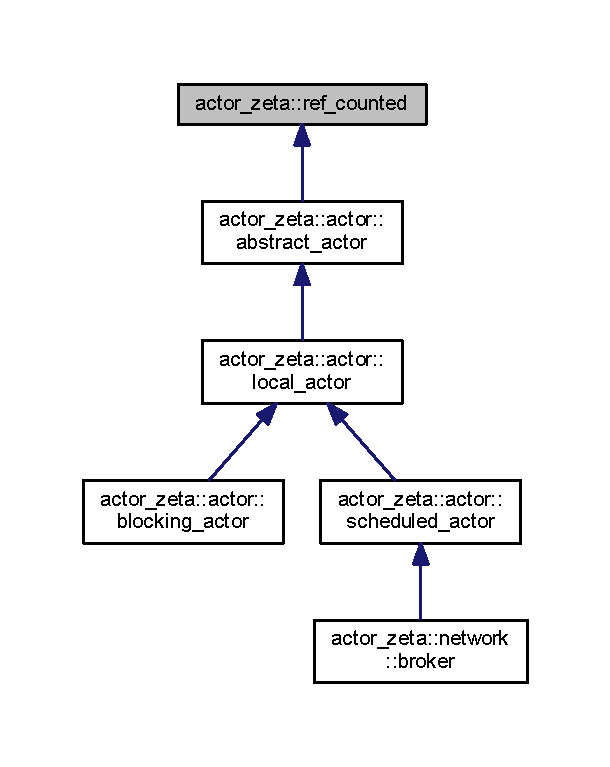
\includegraphics[width=293pt]{classactor__zeta_1_1ref__counted__inherit__graph}
\end{center}
\end{figure}
\subsection*{Public Member Functions}
\begin{DoxyCompactItemize}
\item 
\hyperlink{classactor__zeta_1_1ref__counted_a4e0a85b3b0695a1dc75a393a1b2d7b2e}{$\sim$ref\+\_\+counted} ()
\item 
\hyperlink{classactor__zeta_1_1ref__counted_a8ed09fe39540b2071a9053e812488f0a}{ref\+\_\+counted} ()
\item 
\hyperlink{classactor__zeta_1_1ref__counted_a1832dc33726eac41487e8979e1c2414c}{ref\+\_\+counted} (const \hyperlink{classactor__zeta_1_1ref__counted}{ref\+\_\+counted} \&)
\item 
\hyperlink{classactor__zeta_1_1ref__counted}{ref\+\_\+counted} \& \hyperlink{classactor__zeta_1_1ref__counted_a80302bec44f29ad126c1a04df4a5ce7f}{operator=} (const \hyperlink{classactor__zeta_1_1ref__counted}{ref\+\_\+counted} \&)
\item 
void \hyperlink{classactor__zeta_1_1ref__counted_a46d576dc69eabe39d4c2add161146c23}{ref} () noexcept
\item 
void \hyperlink{classactor__zeta_1_1ref__counted_a3eb2cea75b11216397ac62fbe2101b86}{deref} () noexcept
\item 
bool \hyperlink{classactor__zeta_1_1ref__counted_aa24a0ed9e05d6efc06f8acf879ada836}{unique} () const noexcept
\item 
size\+\_\+t \hyperlink{classactor__zeta_1_1ref__counted_a7fc9ccc71d03d20b3178f45a1ae57713}{get\+\_\+reference\+\_\+count} () const noexcept
\end{DoxyCompactItemize}
\subsection*{Protected Attributes}
\begin{DoxyCompactItemize}
\item 
std\+::atomic$<$ size\+\_\+t $>$ \hyperlink{classactor__zeta_1_1ref__counted_a0af281a31b61d3834cf1a79a81f871a8}{rc\+\_\+}
\end{DoxyCompactItemize}


\subsection{Detailed Description}
This class represents reference counter. 

\subsection{Constructor \& Destructor Documentation}
\mbox{\Hypertarget{classactor__zeta_1_1ref__counted_a4e0a85b3b0695a1dc75a393a1b2d7b2e}\label{classactor__zeta_1_1ref__counted_a4e0a85b3b0695a1dc75a393a1b2d7b2e}} 
\index{actor\+\_\+zeta\+::ref\+\_\+counted@{actor\+\_\+zeta\+::ref\+\_\+counted}!````~ref\+\_\+counted@{$\sim$ref\+\_\+counted}}
\index{````~ref\+\_\+counted@{$\sim$ref\+\_\+counted}!actor\+\_\+zeta\+::ref\+\_\+counted@{actor\+\_\+zeta\+::ref\+\_\+counted}}
\subsubsection{\texorpdfstring{$\sim$ref\+\_\+counted()}{~ref\_counted()}}
{\footnotesize\ttfamily actor\+\_\+zeta\+::ref\+\_\+counted\+::$\sim$ref\+\_\+counted (\begin{DoxyParamCaption}{ }\end{DoxyParamCaption})}

\mbox{\Hypertarget{classactor__zeta_1_1ref__counted_a8ed09fe39540b2071a9053e812488f0a}\label{classactor__zeta_1_1ref__counted_a8ed09fe39540b2071a9053e812488f0a}} 
\index{actor\+\_\+zeta\+::ref\+\_\+counted@{actor\+\_\+zeta\+::ref\+\_\+counted}!ref\+\_\+counted@{ref\+\_\+counted}}
\index{ref\+\_\+counted@{ref\+\_\+counted}!actor\+\_\+zeta\+::ref\+\_\+counted@{actor\+\_\+zeta\+::ref\+\_\+counted}}
\subsubsection{\texorpdfstring{ref\+\_\+counted()}{ref\_counted()}\hspace{0.1cm}{\footnotesize\ttfamily [1/2]}}
{\footnotesize\ttfamily actor\+\_\+zeta\+::ref\+\_\+counted\+::ref\+\_\+counted (\begin{DoxyParamCaption}{ }\end{DoxyParamCaption})}

\mbox{\Hypertarget{classactor__zeta_1_1ref__counted_a1832dc33726eac41487e8979e1c2414c}\label{classactor__zeta_1_1ref__counted_a1832dc33726eac41487e8979e1c2414c}} 
\index{actor\+\_\+zeta\+::ref\+\_\+counted@{actor\+\_\+zeta\+::ref\+\_\+counted}!ref\+\_\+counted@{ref\+\_\+counted}}
\index{ref\+\_\+counted@{ref\+\_\+counted}!actor\+\_\+zeta\+::ref\+\_\+counted@{actor\+\_\+zeta\+::ref\+\_\+counted}}
\subsubsection{\texorpdfstring{ref\+\_\+counted()}{ref\_counted()}\hspace{0.1cm}{\footnotesize\ttfamily [2/2]}}
{\footnotesize\ttfamily actor\+\_\+zeta\+::ref\+\_\+counted\+::ref\+\_\+counted (\begin{DoxyParamCaption}\item[{const \hyperlink{classactor__zeta_1_1ref__counted}{ref\+\_\+counted} \&}]{ }\end{DoxyParamCaption})}



\subsection{Member Function Documentation}
\mbox{\Hypertarget{classactor__zeta_1_1ref__counted_a3eb2cea75b11216397ac62fbe2101b86}\label{classactor__zeta_1_1ref__counted_a3eb2cea75b11216397ac62fbe2101b86}} 
\index{actor\+\_\+zeta\+::ref\+\_\+counted@{actor\+\_\+zeta\+::ref\+\_\+counted}!deref@{deref}}
\index{deref@{deref}!actor\+\_\+zeta\+::ref\+\_\+counted@{actor\+\_\+zeta\+::ref\+\_\+counted}}
\subsubsection{\texorpdfstring{deref()}{deref()}}
{\footnotesize\ttfamily void actor\+\_\+zeta\+::ref\+\_\+counted\+::deref (\begin{DoxyParamCaption}{ }\end{DoxyParamCaption})\hspace{0.3cm}{\ttfamily [noexcept]}}

\mbox{\Hypertarget{classactor__zeta_1_1ref__counted_a7fc9ccc71d03d20b3178f45a1ae57713}\label{classactor__zeta_1_1ref__counted_a7fc9ccc71d03d20b3178f45a1ae57713}} 
\index{actor\+\_\+zeta\+::ref\+\_\+counted@{actor\+\_\+zeta\+::ref\+\_\+counted}!get\+\_\+reference\+\_\+count@{get\+\_\+reference\+\_\+count}}
\index{get\+\_\+reference\+\_\+count@{get\+\_\+reference\+\_\+count}!actor\+\_\+zeta\+::ref\+\_\+counted@{actor\+\_\+zeta\+::ref\+\_\+counted}}
\subsubsection{\texorpdfstring{get\+\_\+reference\+\_\+count()}{get\_reference\_count()}}
{\footnotesize\ttfamily size\+\_\+t actor\+\_\+zeta\+::ref\+\_\+counted\+::get\+\_\+reference\+\_\+count (\begin{DoxyParamCaption}{ }\end{DoxyParamCaption}) const\hspace{0.3cm}{\ttfamily [inline]}, {\ttfamily [noexcept]}}

\mbox{\Hypertarget{classactor__zeta_1_1ref__counted_a80302bec44f29ad126c1a04df4a5ce7f}\label{classactor__zeta_1_1ref__counted_a80302bec44f29ad126c1a04df4a5ce7f}} 
\index{actor\+\_\+zeta\+::ref\+\_\+counted@{actor\+\_\+zeta\+::ref\+\_\+counted}!operator=@{operator=}}
\index{operator=@{operator=}!actor\+\_\+zeta\+::ref\+\_\+counted@{actor\+\_\+zeta\+::ref\+\_\+counted}}
\subsubsection{\texorpdfstring{operator=()}{operator=()}}
{\footnotesize\ttfamily \hyperlink{classactor__zeta_1_1ref__counted}{ref\+\_\+counted} \& actor\+\_\+zeta\+::ref\+\_\+counted\+::operator= (\begin{DoxyParamCaption}\item[{const \hyperlink{classactor__zeta_1_1ref__counted}{ref\+\_\+counted} \&}]{ }\end{DoxyParamCaption})}

\mbox{\Hypertarget{classactor__zeta_1_1ref__counted_a46d576dc69eabe39d4c2add161146c23}\label{classactor__zeta_1_1ref__counted_a46d576dc69eabe39d4c2add161146c23}} 
\index{actor\+\_\+zeta\+::ref\+\_\+counted@{actor\+\_\+zeta\+::ref\+\_\+counted}!ref@{ref}}
\index{ref@{ref}!actor\+\_\+zeta\+::ref\+\_\+counted@{actor\+\_\+zeta\+::ref\+\_\+counted}}
\subsubsection{\texorpdfstring{ref()}{ref()}}
{\footnotesize\ttfamily void actor\+\_\+zeta\+::ref\+\_\+counted\+::ref (\begin{DoxyParamCaption}{ }\end{DoxyParamCaption})\hspace{0.3cm}{\ttfamily [inline]}, {\ttfamily [noexcept]}}

\mbox{\Hypertarget{classactor__zeta_1_1ref__counted_aa24a0ed9e05d6efc06f8acf879ada836}\label{classactor__zeta_1_1ref__counted_aa24a0ed9e05d6efc06f8acf879ada836}} 
\index{actor\+\_\+zeta\+::ref\+\_\+counted@{actor\+\_\+zeta\+::ref\+\_\+counted}!unique@{unique}}
\index{unique@{unique}!actor\+\_\+zeta\+::ref\+\_\+counted@{actor\+\_\+zeta\+::ref\+\_\+counted}}
\subsubsection{\texorpdfstring{unique()}{unique()}}
{\footnotesize\ttfamily bool actor\+\_\+zeta\+::ref\+\_\+counted\+::unique (\begin{DoxyParamCaption}{ }\end{DoxyParamCaption}) const\hspace{0.3cm}{\ttfamily [inline]}, {\ttfamily [noexcept]}}



\subsection{Member Data Documentation}
\mbox{\Hypertarget{classactor__zeta_1_1ref__counted_a0af281a31b61d3834cf1a79a81f871a8}\label{classactor__zeta_1_1ref__counted_a0af281a31b61d3834cf1a79a81f871a8}} 
\index{actor\+\_\+zeta\+::ref\+\_\+counted@{actor\+\_\+zeta\+::ref\+\_\+counted}!rc\+\_\+@{rc\+\_\+}}
\index{rc\+\_\+@{rc\+\_\+}!actor\+\_\+zeta\+::ref\+\_\+counted@{actor\+\_\+zeta\+::ref\+\_\+counted}}
\subsubsection{\texorpdfstring{rc\+\_\+}{rc\_}}
{\footnotesize\ttfamily std\+::atomic$<$size\+\_\+t$>$ actor\+\_\+zeta\+::ref\+\_\+counted\+::rc\+\_\+\hspace{0.3cm}{\ttfamily [protected]}}



The documentation for this class was generated from the following files\+:\begin{DoxyCompactItemize}
\item 
\hyperlink{ref__counted_8hpp}{ref\+\_\+counted.\+hpp}\item 
\hyperlink{ref__counted_8cpp}{ref\+\_\+counted.\+cpp}\end{DoxyCompactItemize}

\hypertarget{classactor__zeta_1_1behavior_1_1request}{}\section{actor\+\_\+zeta\+:\+:behavior\+:\+:request Class Reference}
\label{classactor__zeta_1_1behavior_1_1request}\index{actor\+\_\+zeta\+::behavior\+::request@{actor\+\_\+zeta\+::behavior\+::request}}


This is a request container for messaging.  




{\ttfamily \#include $<$request.\+hpp$>$}

\subsection*{Public Member Functions}
\begin{DoxyCompactItemize}
\item 
\hyperlink{classactor__zeta_1_1behavior_1_1request_aa63a875178ab42de4ad9da3f375e4738}{request} ()=default
\item 
\hyperlink{classactor__zeta_1_1behavior_1_1request_a383424eac1d1c8652c8750d4d6e53f5c}{request} (const \hyperlink{classactor__zeta_1_1behavior_1_1request}{request} \&)=default
\item 
\hyperlink{classactor__zeta_1_1behavior_1_1request}{request} \& \hyperlink{classactor__zeta_1_1behavior_1_1request_adb7544a3e7e43b00f458b794cab09227}{operator=} (const \hyperlink{classactor__zeta_1_1behavior_1_1request}{request} \&)=default
\item 
\hyperlink{classactor__zeta_1_1behavior_1_1request_a815b216b0531fae8e7aa4670fa243176}{request} (\hyperlink{classactor__zeta_1_1behavior_1_1request}{request} \&\&)=default
\item 
\hyperlink{classactor__zeta_1_1behavior_1_1request}{request} \& \hyperlink{classactor__zeta_1_1behavior_1_1request_ae254fec16d1b066e99d56d56a950bbef}{operator=} (\hyperlink{classactor__zeta_1_1behavior_1_1request}{request} \&\&)=default
\item 
\hyperlink{classactor__zeta_1_1behavior_1_1request_a1394a62c51722de66eae954027331d8d}{$\sim$request} ()=default
\item 
\hyperlink{classactor__zeta_1_1behavior_1_1request_ab891918a801fb30cdef7b14737d6945c}{request} (\hyperlink{classactor__zeta_1_1contacts_1_1book__contacts}{contacts\+::book\+\_\+contacts} \&contacts\+\_\+, \hyperlink{classactor__zeta_1_1messaging_1_1message}{messaging\+::message} $\ast$msg)
\item 
\hyperlink{classactor__zeta_1_1messaging_1_1message}{messaging\+::message} $\ast$ \hyperlink{classactor__zeta_1_1behavior_1_1request_a3bd267cd2f121a5b57e616572ddbf762}{message} ()
\item 
\hyperlink{classactor__zeta_1_1contacts_1_1book__contacts}{contacts\+::book\+\_\+contacts} \& \hyperlink{classactor__zeta_1_1behavior_1_1request_ae94a34415643bf735bf6295857f470bf}{contacts} ()
\end{DoxyCompactItemize}


\subsection{Detailed Description}
This is a request container for messaging. 

\subsection{Constructor \& Destructor Documentation}
\mbox{\Hypertarget{classactor__zeta_1_1behavior_1_1request_aa63a875178ab42de4ad9da3f375e4738}\label{classactor__zeta_1_1behavior_1_1request_aa63a875178ab42de4ad9da3f375e4738}} 
\index{actor\+\_\+zeta\+::behavior\+::request@{actor\+\_\+zeta\+::behavior\+::request}!request@{request}}
\index{request@{request}!actor\+\_\+zeta\+::behavior\+::request@{actor\+\_\+zeta\+::behavior\+::request}}
\subsubsection{\texorpdfstring{request()}{request()}\hspace{0.1cm}{\footnotesize\ttfamily [1/4]}}
{\footnotesize\ttfamily actor\+\_\+zeta\+::behavior\+::request\+::request (\begin{DoxyParamCaption}{ }\end{DoxyParamCaption})\hspace{0.3cm}{\ttfamily [default]}}

\mbox{\Hypertarget{classactor__zeta_1_1behavior_1_1request_a383424eac1d1c8652c8750d4d6e53f5c}\label{classactor__zeta_1_1behavior_1_1request_a383424eac1d1c8652c8750d4d6e53f5c}} 
\index{actor\+\_\+zeta\+::behavior\+::request@{actor\+\_\+zeta\+::behavior\+::request}!request@{request}}
\index{request@{request}!actor\+\_\+zeta\+::behavior\+::request@{actor\+\_\+zeta\+::behavior\+::request}}
\subsubsection{\texorpdfstring{request()}{request()}\hspace{0.1cm}{\footnotesize\ttfamily [2/4]}}
{\footnotesize\ttfamily actor\+\_\+zeta\+::behavior\+::request\+::request (\begin{DoxyParamCaption}\item[{const \hyperlink{classactor__zeta_1_1behavior_1_1request}{request} \&}]{ }\end{DoxyParamCaption})\hspace{0.3cm}{\ttfamily [default]}}

\mbox{\Hypertarget{classactor__zeta_1_1behavior_1_1request_a815b216b0531fae8e7aa4670fa243176}\label{classactor__zeta_1_1behavior_1_1request_a815b216b0531fae8e7aa4670fa243176}} 
\index{actor\+\_\+zeta\+::behavior\+::request@{actor\+\_\+zeta\+::behavior\+::request}!request@{request}}
\index{request@{request}!actor\+\_\+zeta\+::behavior\+::request@{actor\+\_\+zeta\+::behavior\+::request}}
\subsubsection{\texorpdfstring{request()}{request()}\hspace{0.1cm}{\footnotesize\ttfamily [3/4]}}
{\footnotesize\ttfamily actor\+\_\+zeta\+::behavior\+::request\+::request (\begin{DoxyParamCaption}\item[{\hyperlink{classactor__zeta_1_1behavior_1_1request}{request} \&\&}]{ }\end{DoxyParamCaption})\hspace{0.3cm}{\ttfamily [default]}}

\mbox{\Hypertarget{classactor__zeta_1_1behavior_1_1request_a1394a62c51722de66eae954027331d8d}\label{classactor__zeta_1_1behavior_1_1request_a1394a62c51722de66eae954027331d8d}} 
\index{actor\+\_\+zeta\+::behavior\+::request@{actor\+\_\+zeta\+::behavior\+::request}!````~request@{$\sim$request}}
\index{````~request@{$\sim$request}!actor\+\_\+zeta\+::behavior\+::request@{actor\+\_\+zeta\+::behavior\+::request}}
\subsubsection{\texorpdfstring{$\sim$request()}{~request()}}
{\footnotesize\ttfamily actor\+\_\+zeta\+::behavior\+::request\+::$\sim$request (\begin{DoxyParamCaption}{ }\end{DoxyParamCaption})\hspace{0.3cm}{\ttfamily [default]}}

\mbox{\Hypertarget{classactor__zeta_1_1behavior_1_1request_ab891918a801fb30cdef7b14737d6945c}\label{classactor__zeta_1_1behavior_1_1request_ab891918a801fb30cdef7b14737d6945c}} 
\index{actor\+\_\+zeta\+::behavior\+::request@{actor\+\_\+zeta\+::behavior\+::request}!request@{request}}
\index{request@{request}!actor\+\_\+zeta\+::behavior\+::request@{actor\+\_\+zeta\+::behavior\+::request}}
\subsubsection{\texorpdfstring{request()}{request()}\hspace{0.1cm}{\footnotesize\ttfamily [4/4]}}
{\footnotesize\ttfamily actor\+\_\+zeta\+::behavior\+::request\+::request (\begin{DoxyParamCaption}\item[{\hyperlink{classactor__zeta_1_1contacts_1_1book__contacts}{contacts\+::book\+\_\+contacts} \&}]{contacts\+\_\+,  }\item[{\hyperlink{classactor__zeta_1_1messaging_1_1message}{messaging\+::message} $\ast$}]{msg }\end{DoxyParamCaption})\hspace{0.3cm}{\ttfamily [inline]}}



\subsection{Member Function Documentation}
\mbox{\Hypertarget{classactor__zeta_1_1behavior_1_1request_ae94a34415643bf735bf6295857f470bf}\label{classactor__zeta_1_1behavior_1_1request_ae94a34415643bf735bf6295857f470bf}} 
\index{actor\+\_\+zeta\+::behavior\+::request@{actor\+\_\+zeta\+::behavior\+::request}!contacts@{contacts}}
\index{contacts@{contacts}!actor\+\_\+zeta\+::behavior\+::request@{actor\+\_\+zeta\+::behavior\+::request}}
\subsubsection{\texorpdfstring{contacts()}{contacts()}}
{\footnotesize\ttfamily \hyperlink{classactor__zeta_1_1contacts_1_1book__contacts}{contacts\+::book\+\_\+contacts}\& actor\+\_\+zeta\+::behavior\+::request\+::contacts (\begin{DoxyParamCaption}{ }\end{DoxyParamCaption})\hspace{0.3cm}{\ttfamily [inline]}}

\mbox{\Hypertarget{classactor__zeta_1_1behavior_1_1request_a3bd267cd2f121a5b57e616572ddbf762}\label{classactor__zeta_1_1behavior_1_1request_a3bd267cd2f121a5b57e616572ddbf762}} 
\index{actor\+\_\+zeta\+::behavior\+::request@{actor\+\_\+zeta\+::behavior\+::request}!message@{message}}
\index{message@{message}!actor\+\_\+zeta\+::behavior\+::request@{actor\+\_\+zeta\+::behavior\+::request}}
\subsubsection{\texorpdfstring{message()}{message()}}
{\footnotesize\ttfamily \hyperlink{classactor__zeta_1_1messaging_1_1message}{messaging\+::message}$\ast$ actor\+\_\+zeta\+::behavior\+::request\+::message (\begin{DoxyParamCaption}{ }\end{DoxyParamCaption})\hspace{0.3cm}{\ttfamily [inline]}}

\mbox{\Hypertarget{classactor__zeta_1_1behavior_1_1request_adb7544a3e7e43b00f458b794cab09227}\label{classactor__zeta_1_1behavior_1_1request_adb7544a3e7e43b00f458b794cab09227}} 
\index{actor\+\_\+zeta\+::behavior\+::request@{actor\+\_\+zeta\+::behavior\+::request}!operator=@{operator=}}
\index{operator=@{operator=}!actor\+\_\+zeta\+::behavior\+::request@{actor\+\_\+zeta\+::behavior\+::request}}
\subsubsection{\texorpdfstring{operator=()}{operator=()}\hspace{0.1cm}{\footnotesize\ttfamily [1/2]}}
{\footnotesize\ttfamily \hyperlink{classactor__zeta_1_1behavior_1_1request}{request}\& actor\+\_\+zeta\+::behavior\+::request\+::operator= (\begin{DoxyParamCaption}\item[{const \hyperlink{classactor__zeta_1_1behavior_1_1request}{request} \&}]{ }\end{DoxyParamCaption})\hspace{0.3cm}{\ttfamily [default]}}

\mbox{\Hypertarget{classactor__zeta_1_1behavior_1_1request_ae254fec16d1b066e99d56d56a950bbef}\label{classactor__zeta_1_1behavior_1_1request_ae254fec16d1b066e99d56d56a950bbef}} 
\index{actor\+\_\+zeta\+::behavior\+::request@{actor\+\_\+zeta\+::behavior\+::request}!operator=@{operator=}}
\index{operator=@{operator=}!actor\+\_\+zeta\+::behavior\+::request@{actor\+\_\+zeta\+::behavior\+::request}}
\subsubsection{\texorpdfstring{operator=()}{operator=()}\hspace{0.1cm}{\footnotesize\ttfamily [2/2]}}
{\footnotesize\ttfamily \hyperlink{classactor__zeta_1_1behavior_1_1request}{request}\& actor\+\_\+zeta\+::behavior\+::request\+::operator= (\begin{DoxyParamCaption}\item[{\hyperlink{classactor__zeta_1_1behavior_1_1request}{request} \&\&}]{ }\end{DoxyParamCaption})\hspace{0.3cm}{\ttfamily [default]}}



The documentation for this class was generated from the following file\+:\begin{DoxyCompactItemize}
\item 
\hyperlink{request_8hpp}{request.\+hpp}\end{DoxyCompactItemize}

\hypertarget{classactor__zeta_1_1behavior_1_1response}{}\section{actor\+\_\+zeta\+:\+:behavior\+:\+:response Class Reference}
\label{classactor__zeta_1_1behavior_1_1response}\index{actor\+\_\+zeta\+::behavior\+::response@{actor\+\_\+zeta\+::behavior\+::response}}


This is a response container for messaging.  




{\ttfamily \#include $<$response.\+hpp$>$}

\subsection*{Public Member Functions}
\begin{DoxyCompactItemize}
\item 
\hyperlink{classactor__zeta_1_1behavior_1_1response_aca59baf848575262bbe2ec9a45fc3295}{response} ()=default
\item 
\hyperlink{classactor__zeta_1_1behavior_1_1response_a52522b1ab1206284c49b774f8f4592b9}{response} (const \hyperlink{classactor__zeta_1_1behavior_1_1response}{response} \&)=default
\item 
\hyperlink{classactor__zeta_1_1behavior_1_1response}{response} \& \hyperlink{classactor__zeta_1_1behavior_1_1response_affcc0aab81cdc00ff9320dd7fe6048ff}{operator=} (const \hyperlink{classactor__zeta_1_1behavior_1_1response}{response} \&)=default
\item 
\hyperlink{classactor__zeta_1_1behavior_1_1response_aa32aab977af64fb95fe7257cfd1bad5b}{response} (\hyperlink{classactor__zeta_1_1behavior_1_1response}{response} \&\&)=default
\item 
\hyperlink{classactor__zeta_1_1behavior_1_1response}{response} \& \hyperlink{classactor__zeta_1_1behavior_1_1response_ad9b1bd1e4aabb899bc196036a111b427}{operator=} (\hyperlink{classactor__zeta_1_1behavior_1_1response}{response} \&\&)=default
\item 
\hyperlink{classactor__zeta_1_1behavior_1_1response_a3b6c18b40faedefdfba5a1d510c2b13e}{$\sim$response} ()=default
\item 
\hyperlink{classactor__zeta_1_1behavior_1_1response_a174f5c5b8ef1a7e6d4f8f0dea9a95c25}{response} (\hyperlink{classactor__zeta_1_1actor_1_1actor__address}{actor\+::actor\+\_\+address} receiver\+\_\+, \hyperlink{classactor__zeta_1_1messaging_1_1message}{messaging\+::message} $\ast$msg)
\item 
\hyperlink{classactor__zeta_1_1messaging_1_1message}{messaging\+::message} $\ast$ \hyperlink{classactor__zeta_1_1behavior_1_1response_a9aa9d35dd338b665fa12ada58b36fe63}{message} ()
\item 
\hyperlink{classactor__zeta_1_1actor_1_1actor__address}{actor\+::actor\+\_\+address} \hyperlink{classactor__zeta_1_1behavior_1_1response_a9735663735901d299d5c8d6ea79005e3}{receiver} () const
\end{DoxyCompactItemize}


\subsection{Detailed Description}
This is a response container for messaging. 

\subsection{Constructor \& Destructor Documentation}
\mbox{\Hypertarget{classactor__zeta_1_1behavior_1_1response_aca59baf848575262bbe2ec9a45fc3295}\label{classactor__zeta_1_1behavior_1_1response_aca59baf848575262bbe2ec9a45fc3295}} 
\index{actor\+\_\+zeta\+::behavior\+::response@{actor\+\_\+zeta\+::behavior\+::response}!response@{response}}
\index{response@{response}!actor\+\_\+zeta\+::behavior\+::response@{actor\+\_\+zeta\+::behavior\+::response}}
\subsubsection{\texorpdfstring{response()}{response()}\hspace{0.1cm}{\footnotesize\ttfamily [1/4]}}
{\footnotesize\ttfamily actor\+\_\+zeta\+::behavior\+::response\+::response (\begin{DoxyParamCaption}{ }\end{DoxyParamCaption})\hspace{0.3cm}{\ttfamily [default]}}

\mbox{\Hypertarget{classactor__zeta_1_1behavior_1_1response_a52522b1ab1206284c49b774f8f4592b9}\label{classactor__zeta_1_1behavior_1_1response_a52522b1ab1206284c49b774f8f4592b9}} 
\index{actor\+\_\+zeta\+::behavior\+::response@{actor\+\_\+zeta\+::behavior\+::response}!response@{response}}
\index{response@{response}!actor\+\_\+zeta\+::behavior\+::response@{actor\+\_\+zeta\+::behavior\+::response}}
\subsubsection{\texorpdfstring{response()}{response()}\hspace{0.1cm}{\footnotesize\ttfamily [2/4]}}
{\footnotesize\ttfamily actor\+\_\+zeta\+::behavior\+::response\+::response (\begin{DoxyParamCaption}\item[{const \hyperlink{classactor__zeta_1_1behavior_1_1response}{response} \&}]{ }\end{DoxyParamCaption})\hspace{0.3cm}{\ttfamily [default]}}

\mbox{\Hypertarget{classactor__zeta_1_1behavior_1_1response_aa32aab977af64fb95fe7257cfd1bad5b}\label{classactor__zeta_1_1behavior_1_1response_aa32aab977af64fb95fe7257cfd1bad5b}} 
\index{actor\+\_\+zeta\+::behavior\+::response@{actor\+\_\+zeta\+::behavior\+::response}!response@{response}}
\index{response@{response}!actor\+\_\+zeta\+::behavior\+::response@{actor\+\_\+zeta\+::behavior\+::response}}
\subsubsection{\texorpdfstring{response()}{response()}\hspace{0.1cm}{\footnotesize\ttfamily [3/4]}}
{\footnotesize\ttfamily actor\+\_\+zeta\+::behavior\+::response\+::response (\begin{DoxyParamCaption}\item[{\hyperlink{classactor__zeta_1_1behavior_1_1response}{response} \&\&}]{ }\end{DoxyParamCaption})\hspace{0.3cm}{\ttfamily [default]}}

\mbox{\Hypertarget{classactor__zeta_1_1behavior_1_1response_a3b6c18b40faedefdfba5a1d510c2b13e}\label{classactor__zeta_1_1behavior_1_1response_a3b6c18b40faedefdfba5a1d510c2b13e}} 
\index{actor\+\_\+zeta\+::behavior\+::response@{actor\+\_\+zeta\+::behavior\+::response}!````~response@{$\sim$response}}
\index{````~response@{$\sim$response}!actor\+\_\+zeta\+::behavior\+::response@{actor\+\_\+zeta\+::behavior\+::response}}
\subsubsection{\texorpdfstring{$\sim$response()}{~response()}}
{\footnotesize\ttfamily actor\+\_\+zeta\+::behavior\+::response\+::$\sim$response (\begin{DoxyParamCaption}{ }\end{DoxyParamCaption})\hspace{0.3cm}{\ttfamily [default]}}

\mbox{\Hypertarget{classactor__zeta_1_1behavior_1_1response_a174f5c5b8ef1a7e6d4f8f0dea9a95c25}\label{classactor__zeta_1_1behavior_1_1response_a174f5c5b8ef1a7e6d4f8f0dea9a95c25}} 
\index{actor\+\_\+zeta\+::behavior\+::response@{actor\+\_\+zeta\+::behavior\+::response}!response@{response}}
\index{response@{response}!actor\+\_\+zeta\+::behavior\+::response@{actor\+\_\+zeta\+::behavior\+::response}}
\subsubsection{\texorpdfstring{response()}{response()}\hspace{0.1cm}{\footnotesize\ttfamily [4/4]}}
{\footnotesize\ttfamily actor\+\_\+zeta\+::behavior\+::response\+::response (\begin{DoxyParamCaption}\item[{\hyperlink{classactor__zeta_1_1actor_1_1actor__address}{actor\+::actor\+\_\+address}}]{receiver\+\_\+,  }\item[{\hyperlink{classactor__zeta_1_1messaging_1_1message}{messaging\+::message} $\ast$}]{msg }\end{DoxyParamCaption})\hspace{0.3cm}{\ttfamily [inline]}}



\subsection{Member Function Documentation}
\mbox{\Hypertarget{classactor__zeta_1_1behavior_1_1response_a9aa9d35dd338b665fa12ada58b36fe63}\label{classactor__zeta_1_1behavior_1_1response_a9aa9d35dd338b665fa12ada58b36fe63}} 
\index{actor\+\_\+zeta\+::behavior\+::response@{actor\+\_\+zeta\+::behavior\+::response}!message@{message}}
\index{message@{message}!actor\+\_\+zeta\+::behavior\+::response@{actor\+\_\+zeta\+::behavior\+::response}}
\subsubsection{\texorpdfstring{message()}{message()}}
{\footnotesize\ttfamily \hyperlink{classactor__zeta_1_1messaging_1_1message}{messaging\+::message}$\ast$ actor\+\_\+zeta\+::behavior\+::response\+::message (\begin{DoxyParamCaption}{ }\end{DoxyParamCaption})\hspace{0.3cm}{\ttfamily [inline]}}

\mbox{\Hypertarget{classactor__zeta_1_1behavior_1_1response_affcc0aab81cdc00ff9320dd7fe6048ff}\label{classactor__zeta_1_1behavior_1_1response_affcc0aab81cdc00ff9320dd7fe6048ff}} 
\index{actor\+\_\+zeta\+::behavior\+::response@{actor\+\_\+zeta\+::behavior\+::response}!operator=@{operator=}}
\index{operator=@{operator=}!actor\+\_\+zeta\+::behavior\+::response@{actor\+\_\+zeta\+::behavior\+::response}}
\subsubsection{\texorpdfstring{operator=()}{operator=()}\hspace{0.1cm}{\footnotesize\ttfamily [1/2]}}
{\footnotesize\ttfamily \hyperlink{classactor__zeta_1_1behavior_1_1response}{response}\& actor\+\_\+zeta\+::behavior\+::response\+::operator= (\begin{DoxyParamCaption}\item[{const \hyperlink{classactor__zeta_1_1behavior_1_1response}{response} \&}]{ }\end{DoxyParamCaption})\hspace{0.3cm}{\ttfamily [default]}}

\mbox{\Hypertarget{classactor__zeta_1_1behavior_1_1response_ad9b1bd1e4aabb899bc196036a111b427}\label{classactor__zeta_1_1behavior_1_1response_ad9b1bd1e4aabb899bc196036a111b427}} 
\index{actor\+\_\+zeta\+::behavior\+::response@{actor\+\_\+zeta\+::behavior\+::response}!operator=@{operator=}}
\index{operator=@{operator=}!actor\+\_\+zeta\+::behavior\+::response@{actor\+\_\+zeta\+::behavior\+::response}}
\subsubsection{\texorpdfstring{operator=()}{operator=()}\hspace{0.1cm}{\footnotesize\ttfamily [2/2]}}
{\footnotesize\ttfamily \hyperlink{classactor__zeta_1_1behavior_1_1response}{response}\& actor\+\_\+zeta\+::behavior\+::response\+::operator= (\begin{DoxyParamCaption}\item[{\hyperlink{classactor__zeta_1_1behavior_1_1response}{response} \&\&}]{ }\end{DoxyParamCaption})\hspace{0.3cm}{\ttfamily [default]}}

\mbox{\Hypertarget{classactor__zeta_1_1behavior_1_1response_a9735663735901d299d5c8d6ea79005e3}\label{classactor__zeta_1_1behavior_1_1response_a9735663735901d299d5c8d6ea79005e3}} 
\index{actor\+\_\+zeta\+::behavior\+::response@{actor\+\_\+zeta\+::behavior\+::response}!receiver@{receiver}}
\index{receiver@{receiver}!actor\+\_\+zeta\+::behavior\+::response@{actor\+\_\+zeta\+::behavior\+::response}}
\subsubsection{\texorpdfstring{receiver()}{receiver()}}
{\footnotesize\ttfamily \hyperlink{classactor__zeta_1_1actor_1_1actor__address}{actor\+::actor\+\_\+address} actor\+\_\+zeta\+::behavior\+::response\+::receiver (\begin{DoxyParamCaption}{ }\end{DoxyParamCaption}) const\hspace{0.3cm}{\ttfamily [inline]}}



The documentation for this class was generated from the following file\+:\begin{DoxyCompactItemize}
\item 
\hyperlink{response_8hpp}{response.\+hpp}\end{DoxyCompactItemize}

\hypertarget{classactor__zeta_1_1actor_1_1scheduled__actor}{}\section{actor\+\_\+zeta\+:\+:actor\+:\+:scheduled\+\_\+actor Class Reference}
\label{classactor__zeta_1_1actor_1_1scheduled__actor}\index{actor\+\_\+zeta\+::actor\+::scheduled\+\_\+actor@{actor\+\_\+zeta\+::actor\+::scheduled\+\_\+actor}}


Represents scheduling type of actor.  




{\ttfamily \#include $<$scheduled\+\_\+actor.\+hpp$>$}



Inheritance diagram for actor\+\_\+zeta\+:\+:actor\+:\+:scheduled\+\_\+actor\+:\nopagebreak
\begin{figure}[H]
\begin{center}
\leavevmode
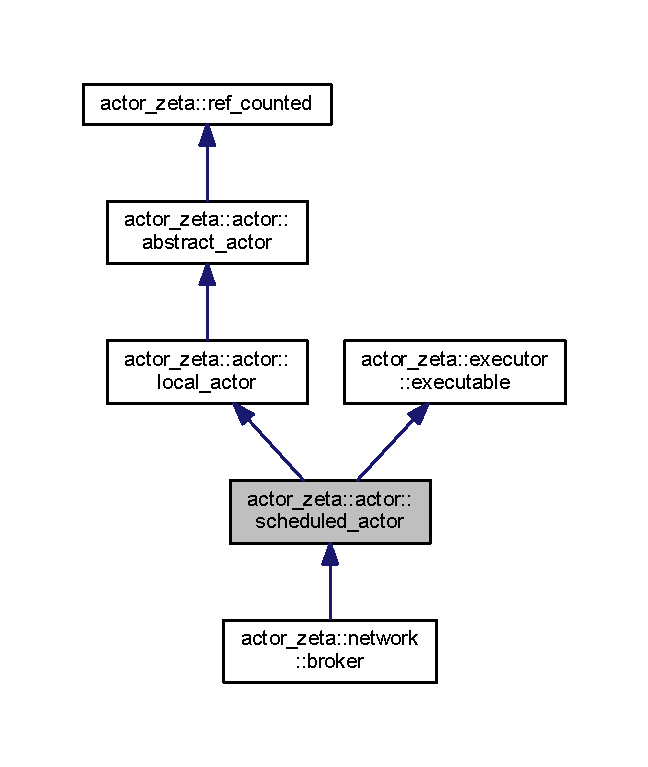
\includegraphics[width=311pt]{classactor__zeta_1_1actor_1_1scheduled__actor__inherit__graph}
\end{center}
\end{figure}


Collaboration diagram for actor\+\_\+zeta\+:\+:actor\+:\+:scheduled\+\_\+actor\+:\nopagebreak
\begin{figure}[H]
\begin{center}
\leavevmode
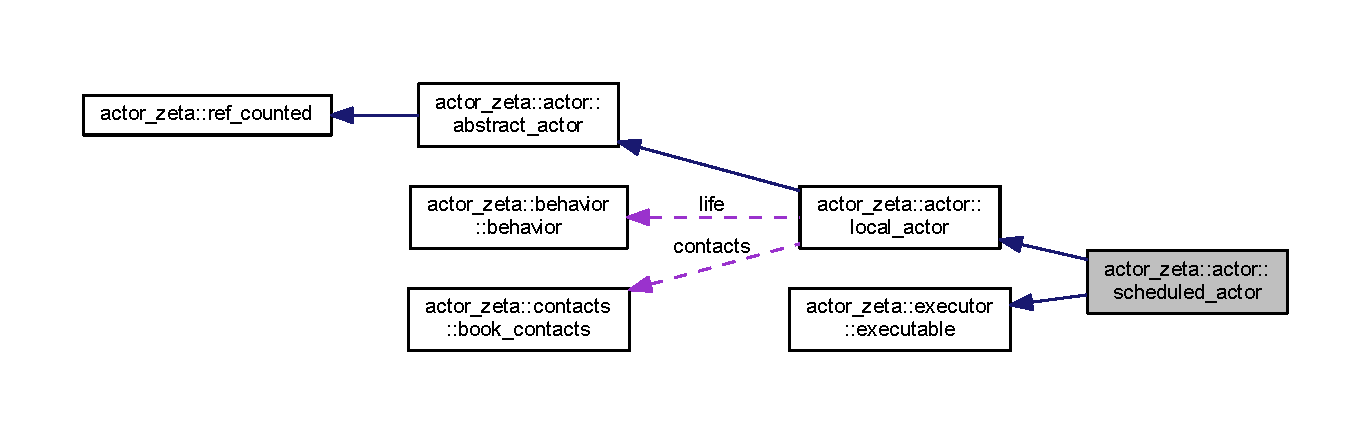
\includegraphics[width=350pt]{classactor__zeta_1_1actor_1_1scheduled__actor__coll__graph}
\end{center}
\end{figure}
\subsection*{Public Member Functions}
\begin{DoxyCompactItemize}
\item 
bool \hyperlink{classactor__zeta_1_1actor_1_1scheduled__actor_acdd757f48a5233a9914209aaf7a2b5ed}{send} (\hyperlink{classactor__zeta_1_1messaging_1_1message}{messaging\+::message} $\ast$) override final
\item 
bool \hyperlink{classactor__zeta_1_1actor_1_1scheduled__actor_a223d20f327713fa65968f909aacb0a32}{send} (\hyperlink{classactor__zeta_1_1messaging_1_1message}{messaging\+::message} $\ast$, \hyperlink{structactor__zeta_1_1executor_1_1execution__device}{executor\+::execution\+\_\+device} $\ast$) override final
\item 
void \hyperlink{classactor__zeta_1_1actor_1_1scheduled__actor_a15dcbee3ab1540c7ed675846cbf10726}{launch} (\hyperlink{structactor__zeta_1_1executor_1_1execution__device}{executor\+::execution\+\_\+device} $\ast$, bool) override final
\item 
\hyperlink{structactor__zeta_1_1executor_1_1executable_aef06c63be7b22b021ade4b83ed4f3cc4}{executor\+::executable\+::executable\+\_\+result} \hyperlink{classactor__zeta_1_1actor_1_1scheduled__actor_a9031c2f3ff6c8c62698b53fa92e56274}{run} (\hyperlink{structactor__zeta_1_1executor_1_1execution__device}{executor\+::execution\+\_\+device} $\ast$, size\+\_\+t max\+\_\+throughput) override final
\end{DoxyCompactItemize}
\subsection*{Protected Member Functions}
\begin{DoxyCompactItemize}
\item 
\hyperlink{classactor__zeta_1_1actor_1_1scheduled__actor_a67ec95fe272be22dd146da79d067feaa}{scheduled\+\_\+actor} (\hyperlink{classactor__zeta_1_1environment_1_1environment}{environment\+::environment} $\ast$, const std\+::string \&)
\item 
void \hyperlink{classactor__zeta_1_1actor_1_1scheduled__actor_a760f7fedcd61cae392c435a13bcab50c}{attach\+\_\+to\+\_\+scheduler} () override final
\item 
void \hyperlink{classactor__zeta_1_1actor_1_1scheduled__actor_aaf6582fc27718071ff7c9d516b8f0cf6}{detach\+\_\+from\+\_\+scheduler} () override final
\end{DoxyCompactItemize}
\subsection*{Additional Inherited Members}


\subsection{Detailed Description}
Represents scheduling type of actor. 

\subsection{Constructor \& Destructor Documentation}
\mbox{\Hypertarget{classactor__zeta_1_1actor_1_1scheduled__actor_a67ec95fe272be22dd146da79d067feaa}\label{classactor__zeta_1_1actor_1_1scheduled__actor_a67ec95fe272be22dd146da79d067feaa}} 
\index{actor\+\_\+zeta\+::actor\+::scheduled\+\_\+actor@{actor\+\_\+zeta\+::actor\+::scheduled\+\_\+actor}!scheduled\+\_\+actor@{scheduled\+\_\+actor}}
\index{scheduled\+\_\+actor@{scheduled\+\_\+actor}!actor\+\_\+zeta\+::actor\+::scheduled\+\_\+actor@{actor\+\_\+zeta\+::actor\+::scheduled\+\_\+actor}}
\subsubsection{\texorpdfstring{scheduled\+\_\+actor()}{scheduled\_actor()}}
{\footnotesize\ttfamily actor\+\_\+zeta\+::actor\+::scheduled\+\_\+actor\+::scheduled\+\_\+actor (\begin{DoxyParamCaption}\item[{\hyperlink{classactor__zeta_1_1environment_1_1environment}{environment\+::environment} $\ast$}]{env,  }\item[{const std\+::string \&}]{name }\end{DoxyParamCaption})\hspace{0.3cm}{\ttfamily [protected]}}



\subsection{Member Function Documentation}
\mbox{\Hypertarget{classactor__zeta_1_1actor_1_1scheduled__actor_a760f7fedcd61cae392c435a13bcab50c}\label{classactor__zeta_1_1actor_1_1scheduled__actor_a760f7fedcd61cae392c435a13bcab50c}} 
\index{actor\+\_\+zeta\+::actor\+::scheduled\+\_\+actor@{actor\+\_\+zeta\+::actor\+::scheduled\+\_\+actor}!attach\+\_\+to\+\_\+scheduler@{attach\+\_\+to\+\_\+scheduler}}
\index{attach\+\_\+to\+\_\+scheduler@{attach\+\_\+to\+\_\+scheduler}!actor\+\_\+zeta\+::actor\+::scheduled\+\_\+actor@{actor\+\_\+zeta\+::actor\+::scheduled\+\_\+actor}}
\subsubsection{\texorpdfstring{attach\+\_\+to\+\_\+scheduler()}{attach\_to\_scheduler()}}
{\footnotesize\ttfamily void actor\+\_\+zeta\+::actor\+::scheduled\+\_\+actor\+::attach\+\_\+to\+\_\+scheduler (\begin{DoxyParamCaption}{ }\end{DoxyParamCaption})\hspace{0.3cm}{\ttfamily [final]}, {\ttfamily [override]}, {\ttfamily [protected]}, {\ttfamily [virtual]}}



Implements \hyperlink{structactor__zeta_1_1executor_1_1executable_a35557044e3f8d17504a66628aeea1cee}{actor\+\_\+zeta\+::executor\+::executable}.

\mbox{\Hypertarget{classactor__zeta_1_1actor_1_1scheduled__actor_aaf6582fc27718071ff7c9d516b8f0cf6}\label{classactor__zeta_1_1actor_1_1scheduled__actor_aaf6582fc27718071ff7c9d516b8f0cf6}} 
\index{actor\+\_\+zeta\+::actor\+::scheduled\+\_\+actor@{actor\+\_\+zeta\+::actor\+::scheduled\+\_\+actor}!detach\+\_\+from\+\_\+scheduler@{detach\+\_\+from\+\_\+scheduler}}
\index{detach\+\_\+from\+\_\+scheduler@{detach\+\_\+from\+\_\+scheduler}!actor\+\_\+zeta\+::actor\+::scheduled\+\_\+actor@{actor\+\_\+zeta\+::actor\+::scheduled\+\_\+actor}}
\subsubsection{\texorpdfstring{detach\+\_\+from\+\_\+scheduler()}{detach\_from\_scheduler()}}
{\footnotesize\ttfamily void actor\+\_\+zeta\+::actor\+::scheduled\+\_\+actor\+::detach\+\_\+from\+\_\+scheduler (\begin{DoxyParamCaption}{ }\end{DoxyParamCaption})\hspace{0.3cm}{\ttfamily [final]}, {\ttfamily [override]}, {\ttfamily [protected]}, {\ttfamily [virtual]}}



Implements \hyperlink{structactor__zeta_1_1executor_1_1executable_a2fe91b45b919fc6f3fce21e64d2c1f91}{actor\+\_\+zeta\+::executor\+::executable}.

\mbox{\Hypertarget{classactor__zeta_1_1actor_1_1scheduled__actor_a15dcbee3ab1540c7ed675846cbf10726}\label{classactor__zeta_1_1actor_1_1scheduled__actor_a15dcbee3ab1540c7ed675846cbf10726}} 
\index{actor\+\_\+zeta\+::actor\+::scheduled\+\_\+actor@{actor\+\_\+zeta\+::actor\+::scheduled\+\_\+actor}!launch@{launch}}
\index{launch@{launch}!actor\+\_\+zeta\+::actor\+::scheduled\+\_\+actor@{actor\+\_\+zeta\+::actor\+::scheduled\+\_\+actor}}
\subsubsection{\texorpdfstring{launch()}{launch()}}
{\footnotesize\ttfamily void actor\+\_\+zeta\+::actor\+::scheduled\+\_\+actor\+::launch (\begin{DoxyParamCaption}\item[{\hyperlink{structactor__zeta_1_1executor_1_1execution__device}{executor\+::execution\+\_\+device} $\ast$}]{e,  }\item[{bool}]{hide }\end{DoxyParamCaption})\hspace{0.3cm}{\ttfamily [final]}, {\ttfamily [override]}, {\ttfamily [virtual]}}



Implements \hyperlink{classactor__zeta_1_1actor_1_1local__actor_acfba412b813aee3250c589bee232f3cd}{actor\+\_\+zeta\+::actor\+::local\+\_\+actor}.

\mbox{\Hypertarget{classactor__zeta_1_1actor_1_1scheduled__actor_a9031c2f3ff6c8c62698b53fa92e56274}\label{classactor__zeta_1_1actor_1_1scheduled__actor_a9031c2f3ff6c8c62698b53fa92e56274}} 
\index{actor\+\_\+zeta\+::actor\+::scheduled\+\_\+actor@{actor\+\_\+zeta\+::actor\+::scheduled\+\_\+actor}!run@{run}}
\index{run@{run}!actor\+\_\+zeta\+::actor\+::scheduled\+\_\+actor@{actor\+\_\+zeta\+::actor\+::scheduled\+\_\+actor}}
\subsubsection{\texorpdfstring{run()}{run()}}
{\footnotesize\ttfamily \hyperlink{structactor__zeta_1_1executor_1_1executable_aef06c63be7b22b021ade4b83ed4f3cc4}{executor\+::executable\+::executable\+\_\+result} actor\+\_\+zeta\+::actor\+::scheduled\+\_\+actor\+::run (\begin{DoxyParamCaption}\item[{\hyperlink{structactor__zeta_1_1executor_1_1execution__device}{executor\+::execution\+\_\+device} $\ast$}]{e,  }\item[{size\+\_\+t}]{max\+\_\+throughput }\end{DoxyParamCaption})\hspace{0.3cm}{\ttfamily [final]}, {\ttfamily [override]}, {\ttfamily [virtual]}}



Implements \hyperlink{structactor__zeta_1_1executor_1_1executable_a61d6cbce8b124e1e5ef80f8befea2a89}{actor\+\_\+zeta\+::executor\+::executable}.

\mbox{\Hypertarget{classactor__zeta_1_1actor_1_1scheduled__actor_acdd757f48a5233a9914209aaf7a2b5ed}\label{classactor__zeta_1_1actor_1_1scheduled__actor_acdd757f48a5233a9914209aaf7a2b5ed}} 
\index{actor\+\_\+zeta\+::actor\+::scheduled\+\_\+actor@{actor\+\_\+zeta\+::actor\+::scheduled\+\_\+actor}!send@{send}}
\index{send@{send}!actor\+\_\+zeta\+::actor\+::scheduled\+\_\+actor@{actor\+\_\+zeta\+::actor\+::scheduled\+\_\+actor}}
\subsubsection{\texorpdfstring{send()}{send()}\hspace{0.1cm}{\footnotesize\ttfamily [1/2]}}
{\footnotesize\ttfamily bool actor\+\_\+zeta\+::actor\+::scheduled\+\_\+actor\+::send (\begin{DoxyParamCaption}\item[{\hyperlink{classactor__zeta_1_1messaging_1_1message}{messaging\+::message} $\ast$}]{msg }\end{DoxyParamCaption})\hspace{0.3cm}{\ttfamily [final]}, {\ttfamily [override]}, {\ttfamily [virtual]}}



Implements \hyperlink{classactor__zeta_1_1actor_1_1abstract__actor_a9316a5088e53255d74ade831e1fcfb47}{actor\+\_\+zeta\+::actor\+::abstract\+\_\+actor}.

\mbox{\Hypertarget{classactor__zeta_1_1actor_1_1scheduled__actor_a223d20f327713fa65968f909aacb0a32}\label{classactor__zeta_1_1actor_1_1scheduled__actor_a223d20f327713fa65968f909aacb0a32}} 
\index{actor\+\_\+zeta\+::actor\+::scheduled\+\_\+actor@{actor\+\_\+zeta\+::actor\+::scheduled\+\_\+actor}!send@{send}}
\index{send@{send}!actor\+\_\+zeta\+::actor\+::scheduled\+\_\+actor@{actor\+\_\+zeta\+::actor\+::scheduled\+\_\+actor}}
\subsubsection{\texorpdfstring{send()}{send()}\hspace{0.1cm}{\footnotesize\ttfamily [2/2]}}
{\footnotesize\ttfamily bool actor\+\_\+zeta\+::actor\+::scheduled\+\_\+actor\+::send (\begin{DoxyParamCaption}\item[{\hyperlink{classactor__zeta_1_1messaging_1_1message}{messaging\+::message} $\ast$}]{mep,  }\item[{\hyperlink{structactor__zeta_1_1executor_1_1execution__device}{executor\+::execution\+\_\+device} $\ast$}]{e }\end{DoxyParamCaption})\hspace{0.3cm}{\ttfamily [final]}, {\ttfamily [override]}, {\ttfamily [virtual]}}



Implements \hyperlink{classactor__zeta_1_1actor_1_1abstract__actor_a929d99bea25095035695bad6e6516575}{actor\+\_\+zeta\+::actor\+::abstract\+\_\+actor}.



The documentation for this class was generated from the following files\+:\begin{DoxyCompactItemize}
\item 
\hyperlink{scheduled__actor_8hpp}{scheduled\+\_\+actor.\+hpp}\item 
\hyperlink{scheduled__actor_8cpp}{scheduled\+\_\+actor.\+cpp}\end{DoxyCompactItemize}

\hypertarget{classactor__zeta_1_1environment_1_1shared__group}{}\section{actor\+\_\+zeta\+:\+:environment\+:\+:shared\+\_\+group Class Reference}
\label{classactor__zeta_1_1environment_1_1shared__group}\index{actor\+\_\+zeta\+::environment\+::shared\+\_\+group@{actor\+\_\+zeta\+::environment\+::shared\+\_\+group}}


Group realisation with common resource.  




{\ttfamily \#include $<$shared\+\_\+group.\+hpp$>$}

\subsection*{Public Member Functions}
\begin{DoxyCompactItemize}
\item 
\hyperlink{classactor__zeta_1_1environment_1_1shared__group_aee1d8b2f8b57f7e770c19a514cc492f0}{shared\+\_\+group} ()=default
\item 
\hyperlink{classactor__zeta_1_1environment_1_1shared__group_a72a67c42ad9a0632f485055a06e8c455}{shared\+\_\+group} (const \hyperlink{classactor__zeta_1_1environment_1_1shared__group}{shared\+\_\+group} \&)=delete
\item 
\hyperlink{classactor__zeta_1_1environment_1_1shared__group_a646165cadc164fd66152a5b95f09f2e6}{shared\+\_\+group} (\hyperlink{classactor__zeta_1_1environment_1_1shared__group}{shared\+\_\+group} \&\&)=default
\item 
\hyperlink{classactor__zeta_1_1environment_1_1shared__group}{shared\+\_\+group} \& \hyperlink{classactor__zeta_1_1environment_1_1shared__group_a9dcb7f4adcad7c66ac43d65b5800f24d}{operator=} (const \hyperlink{classactor__zeta_1_1environment_1_1shared__group}{shared\+\_\+group} \&)=delete
\item 
\hyperlink{classactor__zeta_1_1environment_1_1shared__group}{shared\+\_\+group} \& \hyperlink{classactor__zeta_1_1environment_1_1shared__group_a00439854585c059d8e4e0fc29ae8c5da}{operator=} (\hyperlink{classactor__zeta_1_1environment_1_1shared__group}{shared\+\_\+group} \&\&)=default
\item 
\hyperlink{classactor__zeta_1_1environment_1_1shared__group_ab77aacd00268bffe1f97fa51d1979d3a}{$\sim$shared\+\_\+group} ()=default
\item 
void \hyperlink{classactor__zeta_1_1environment_1_1shared__group_a70dd0c4545246a60f45f9cba3734720e}{add} (\hyperlink{classactor__zeta_1_1actor_1_1abstract__actor}{actor\+::abstract\+\_\+actor} $\ast$)
\item 
void \hyperlink{classactor__zeta_1_1environment_1_1shared__group_a92fa230ff67cd97226ba57efb43472e2}{send\+\_\+current} (const std\+::string \&, \hyperlink{classactor__zeta_1_1messaging_1_1message}{messaging\+::message} $\ast$)
\item 
void \hyperlink{classactor__zeta_1_1environment_1_1shared__group_ab74c04703451bceb0c517ca5fd4d8e05}{send\+\_\+all} (\hyperlink{classactor__zeta_1_1messaging_1_1message}{messaging\+::message} $\ast$)
\end{DoxyCompactItemize}


\subsection{Detailed Description}
Group realisation with common resource. 

\subsection{Constructor \& Destructor Documentation}
\mbox{\Hypertarget{classactor__zeta_1_1environment_1_1shared__group_aee1d8b2f8b57f7e770c19a514cc492f0}\label{classactor__zeta_1_1environment_1_1shared__group_aee1d8b2f8b57f7e770c19a514cc492f0}} 
\index{actor\+\_\+zeta\+::environment\+::shared\+\_\+group@{actor\+\_\+zeta\+::environment\+::shared\+\_\+group}!shared\+\_\+group@{shared\+\_\+group}}
\index{shared\+\_\+group@{shared\+\_\+group}!actor\+\_\+zeta\+::environment\+::shared\+\_\+group@{actor\+\_\+zeta\+::environment\+::shared\+\_\+group}}
\subsubsection{\texorpdfstring{shared\+\_\+group()}{shared\_group()}\hspace{0.1cm}{\footnotesize\ttfamily [1/3]}}
{\footnotesize\ttfamily actor\+\_\+zeta\+::environment\+::shared\+\_\+group\+::shared\+\_\+group (\begin{DoxyParamCaption}{ }\end{DoxyParamCaption})\hspace{0.3cm}{\ttfamily [default]}}

\mbox{\Hypertarget{classactor__zeta_1_1environment_1_1shared__group_a72a67c42ad9a0632f485055a06e8c455}\label{classactor__zeta_1_1environment_1_1shared__group_a72a67c42ad9a0632f485055a06e8c455}} 
\index{actor\+\_\+zeta\+::environment\+::shared\+\_\+group@{actor\+\_\+zeta\+::environment\+::shared\+\_\+group}!shared\+\_\+group@{shared\+\_\+group}}
\index{shared\+\_\+group@{shared\+\_\+group}!actor\+\_\+zeta\+::environment\+::shared\+\_\+group@{actor\+\_\+zeta\+::environment\+::shared\+\_\+group}}
\subsubsection{\texorpdfstring{shared\+\_\+group()}{shared\_group()}\hspace{0.1cm}{\footnotesize\ttfamily [2/3]}}
{\footnotesize\ttfamily actor\+\_\+zeta\+::environment\+::shared\+\_\+group\+::shared\+\_\+group (\begin{DoxyParamCaption}\item[{const \hyperlink{classactor__zeta_1_1environment_1_1shared__group}{shared\+\_\+group} \&}]{ }\end{DoxyParamCaption})\hspace{0.3cm}{\ttfamily [delete]}}

\mbox{\Hypertarget{classactor__zeta_1_1environment_1_1shared__group_a646165cadc164fd66152a5b95f09f2e6}\label{classactor__zeta_1_1environment_1_1shared__group_a646165cadc164fd66152a5b95f09f2e6}} 
\index{actor\+\_\+zeta\+::environment\+::shared\+\_\+group@{actor\+\_\+zeta\+::environment\+::shared\+\_\+group}!shared\+\_\+group@{shared\+\_\+group}}
\index{shared\+\_\+group@{shared\+\_\+group}!actor\+\_\+zeta\+::environment\+::shared\+\_\+group@{actor\+\_\+zeta\+::environment\+::shared\+\_\+group}}
\subsubsection{\texorpdfstring{shared\+\_\+group()}{shared\_group()}\hspace{0.1cm}{\footnotesize\ttfamily [3/3]}}
{\footnotesize\ttfamily actor\+\_\+zeta\+::environment\+::shared\+\_\+group\+::shared\+\_\+group (\begin{DoxyParamCaption}\item[{\hyperlink{classactor__zeta_1_1environment_1_1shared__group}{shared\+\_\+group} \&\&}]{ }\end{DoxyParamCaption})\hspace{0.3cm}{\ttfamily [default]}}

\mbox{\Hypertarget{classactor__zeta_1_1environment_1_1shared__group_ab77aacd00268bffe1f97fa51d1979d3a}\label{classactor__zeta_1_1environment_1_1shared__group_ab77aacd00268bffe1f97fa51d1979d3a}} 
\index{actor\+\_\+zeta\+::environment\+::shared\+\_\+group@{actor\+\_\+zeta\+::environment\+::shared\+\_\+group}!````~shared\+\_\+group@{$\sim$shared\+\_\+group}}
\index{````~shared\+\_\+group@{$\sim$shared\+\_\+group}!actor\+\_\+zeta\+::environment\+::shared\+\_\+group@{actor\+\_\+zeta\+::environment\+::shared\+\_\+group}}
\subsubsection{\texorpdfstring{$\sim$shared\+\_\+group()}{~shared\_group()}}
{\footnotesize\ttfamily actor\+\_\+zeta\+::environment\+::shared\+\_\+group\+::$\sim$shared\+\_\+group (\begin{DoxyParamCaption}{ }\end{DoxyParamCaption})\hspace{0.3cm}{\ttfamily [default]}}



\subsection{Member Function Documentation}
\mbox{\Hypertarget{classactor__zeta_1_1environment_1_1shared__group_a70dd0c4545246a60f45f9cba3734720e}\label{classactor__zeta_1_1environment_1_1shared__group_a70dd0c4545246a60f45f9cba3734720e}} 
\index{actor\+\_\+zeta\+::environment\+::shared\+\_\+group@{actor\+\_\+zeta\+::environment\+::shared\+\_\+group}!add@{add}}
\index{add@{add}!actor\+\_\+zeta\+::environment\+::shared\+\_\+group@{actor\+\_\+zeta\+::environment\+::shared\+\_\+group}}
\subsubsection{\texorpdfstring{add()}{add()}}
{\footnotesize\ttfamily void actor\+\_\+zeta\+::environment\+::shared\+\_\+group\+::add (\begin{DoxyParamCaption}\item[{\hyperlink{classactor__zeta_1_1actor_1_1abstract__actor}{actor\+::abstract\+\_\+actor} $\ast$}]{a }\end{DoxyParamCaption})}

\mbox{\Hypertarget{classactor__zeta_1_1environment_1_1shared__group_a9dcb7f4adcad7c66ac43d65b5800f24d}\label{classactor__zeta_1_1environment_1_1shared__group_a9dcb7f4adcad7c66ac43d65b5800f24d}} 
\index{actor\+\_\+zeta\+::environment\+::shared\+\_\+group@{actor\+\_\+zeta\+::environment\+::shared\+\_\+group}!operator=@{operator=}}
\index{operator=@{operator=}!actor\+\_\+zeta\+::environment\+::shared\+\_\+group@{actor\+\_\+zeta\+::environment\+::shared\+\_\+group}}
\subsubsection{\texorpdfstring{operator=()}{operator=()}\hspace{0.1cm}{\footnotesize\ttfamily [1/2]}}
{\footnotesize\ttfamily \hyperlink{classactor__zeta_1_1environment_1_1shared__group}{shared\+\_\+group}\& actor\+\_\+zeta\+::environment\+::shared\+\_\+group\+::operator= (\begin{DoxyParamCaption}\item[{const \hyperlink{classactor__zeta_1_1environment_1_1shared__group}{shared\+\_\+group} \&}]{ }\end{DoxyParamCaption})\hspace{0.3cm}{\ttfamily [delete]}}

\mbox{\Hypertarget{classactor__zeta_1_1environment_1_1shared__group_a00439854585c059d8e4e0fc29ae8c5da}\label{classactor__zeta_1_1environment_1_1shared__group_a00439854585c059d8e4e0fc29ae8c5da}} 
\index{actor\+\_\+zeta\+::environment\+::shared\+\_\+group@{actor\+\_\+zeta\+::environment\+::shared\+\_\+group}!operator=@{operator=}}
\index{operator=@{operator=}!actor\+\_\+zeta\+::environment\+::shared\+\_\+group@{actor\+\_\+zeta\+::environment\+::shared\+\_\+group}}
\subsubsection{\texorpdfstring{operator=()}{operator=()}\hspace{0.1cm}{\footnotesize\ttfamily [2/2]}}
{\footnotesize\ttfamily \hyperlink{classactor__zeta_1_1environment_1_1shared__group}{shared\+\_\+group}\& actor\+\_\+zeta\+::environment\+::shared\+\_\+group\+::operator= (\begin{DoxyParamCaption}\item[{\hyperlink{classactor__zeta_1_1environment_1_1shared__group}{shared\+\_\+group} \&\&}]{ }\end{DoxyParamCaption})\hspace{0.3cm}{\ttfamily [default]}}

\mbox{\Hypertarget{classactor__zeta_1_1environment_1_1shared__group_ab74c04703451bceb0c517ca5fd4d8e05}\label{classactor__zeta_1_1environment_1_1shared__group_ab74c04703451bceb0c517ca5fd4d8e05}} 
\index{actor\+\_\+zeta\+::environment\+::shared\+\_\+group@{actor\+\_\+zeta\+::environment\+::shared\+\_\+group}!send\+\_\+all@{send\+\_\+all}}
\index{send\+\_\+all@{send\+\_\+all}!actor\+\_\+zeta\+::environment\+::shared\+\_\+group@{actor\+\_\+zeta\+::environment\+::shared\+\_\+group}}
\subsubsection{\texorpdfstring{send\+\_\+all()}{send\_all()}}
{\footnotesize\ttfamily void actor\+\_\+zeta\+::environment\+::shared\+\_\+group\+::send\+\_\+all (\begin{DoxyParamCaption}\item[{\hyperlink{classactor__zeta_1_1messaging_1_1message}{messaging\+::message} $\ast$}]{msg }\end{DoxyParamCaption})}

\mbox{\Hypertarget{classactor__zeta_1_1environment_1_1shared__group_a92fa230ff67cd97226ba57efb43472e2}\label{classactor__zeta_1_1environment_1_1shared__group_a92fa230ff67cd97226ba57efb43472e2}} 
\index{actor\+\_\+zeta\+::environment\+::shared\+\_\+group@{actor\+\_\+zeta\+::environment\+::shared\+\_\+group}!send\+\_\+current@{send\+\_\+current}}
\index{send\+\_\+current@{send\+\_\+current}!actor\+\_\+zeta\+::environment\+::shared\+\_\+group@{actor\+\_\+zeta\+::environment\+::shared\+\_\+group}}
\subsubsection{\texorpdfstring{send\+\_\+current()}{send\_current()}}
{\footnotesize\ttfamily void actor\+\_\+zeta\+::environment\+::shared\+\_\+group\+::send\+\_\+current (\begin{DoxyParamCaption}\item[{const std\+::string \&}]{name,  }\item[{\hyperlink{classactor__zeta_1_1messaging_1_1message}{messaging\+::message} $\ast$}]{msg }\end{DoxyParamCaption})}



The documentation for this class was generated from the following files\+:\begin{DoxyCompactItemize}
\item 
\hyperlink{shared__group_8hpp}{shared\+\_\+group.\+hpp}\item 
\hyperlink{shared__group_8cpp}{shared\+\_\+group.\+cpp}\end{DoxyCompactItemize}

\hypertarget{classactor__zeta_1_1skip}{}\section{actor\+\_\+zeta\+:\+:skip Class Reference}
\label{classactor__zeta_1_1skip}\index{actor\+\_\+zeta\+::skip@{actor\+\_\+zeta\+::skip}}


A class used for skipping action.  




{\ttfamily \#include $<$skip.\+hpp$>$}



Inheritance diagram for actor\+\_\+zeta\+:\+:skip\+:\nopagebreak
\begin{figure}[H]
\begin{center}
\leavevmode
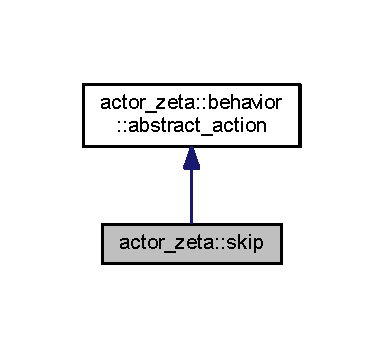
\includegraphics[width=184pt]{classactor__zeta_1_1skip__inherit__graph}
\end{center}
\end{figure}


Collaboration diagram for actor\+\_\+zeta\+:\+:skip\+:\nopagebreak
\begin{figure}[H]
\begin{center}
\leavevmode
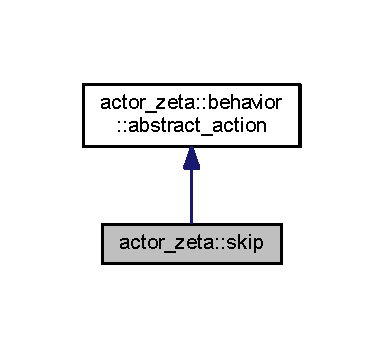
\includegraphics[width=184pt]{classactor__zeta_1_1skip__coll__graph}
\end{center}
\end{figure}
\subsection*{Public Member Functions}
\begin{DoxyCompactItemize}
\item 
\hyperlink{classactor__zeta_1_1skip_a2a649385cc43b90561bbd106aadf55fe}{skip} ()
\item 
\hyperlink{classactor__zeta_1_1behavior_1_1response}{behavior\+::response} $\ast$ \hyperlink{classactor__zeta_1_1skip_a0a674c6ce55d365b2bae8ec19a58e29f}{operator()} (\hyperlink{classactor__zeta_1_1behavior_1_1request}{behavior\+::request} $\ast$) override final
\end{DoxyCompactItemize}


\subsection{Detailed Description}
A class used for skipping action. 

\subsection{Constructor \& Destructor Documentation}
\mbox{\Hypertarget{classactor__zeta_1_1skip_a2a649385cc43b90561bbd106aadf55fe}\label{classactor__zeta_1_1skip_a2a649385cc43b90561bbd106aadf55fe}} 
\index{actor\+\_\+zeta\+::skip@{actor\+\_\+zeta\+::skip}!skip@{skip}}
\index{skip@{skip}!actor\+\_\+zeta\+::skip@{actor\+\_\+zeta\+::skip}}
\subsubsection{\texorpdfstring{skip()}{skip()}}
{\footnotesize\ttfamily actor\+\_\+zeta\+::skip\+::skip (\begin{DoxyParamCaption}{ }\end{DoxyParamCaption})}



\subsection{Member Function Documentation}
\mbox{\Hypertarget{classactor__zeta_1_1skip_a0a674c6ce55d365b2bae8ec19a58e29f}\label{classactor__zeta_1_1skip_a0a674c6ce55d365b2bae8ec19a58e29f}} 
\index{actor\+\_\+zeta\+::skip@{actor\+\_\+zeta\+::skip}!operator()@{operator()}}
\index{operator()@{operator()}!actor\+\_\+zeta\+::skip@{actor\+\_\+zeta\+::skip}}
\subsubsection{\texorpdfstring{operator()()}{operator()()}}
{\footnotesize\ttfamily \hyperlink{classactor__zeta_1_1behavior_1_1response}{behavior\+::response} $\ast$ actor\+\_\+zeta\+::skip\+::operator() (\begin{DoxyParamCaption}\item[{\hyperlink{classactor__zeta_1_1behavior_1_1request}{behavior\+::request} $\ast$}]{r }\end{DoxyParamCaption})\hspace{0.3cm}{\ttfamily [final]}, {\ttfamily [override]}, {\ttfamily [virtual]}}



Implements \hyperlink{classactor__zeta_1_1behavior_1_1abstract__action_a5e48075d77fbd93615fc9b757e6a4d87}{actor\+\_\+zeta\+::behavior\+::abstract\+\_\+action}.



The documentation for this class was generated from the following files\+:\begin{DoxyCompactItemize}
\item 
\hyperlink{skip_8hpp}{skip.\+hpp}\item 
\hyperlink{skip_8cpp}{skip.\+cpp}\end{DoxyCompactItemize}

\hypertarget{classactor__zeta_1_1sync__contacts}{}\section{actor\+\_\+zeta\+:\+:sync\+\_\+contacts Class Reference}
\label{classactor__zeta_1_1sync__contacts}\index{actor\+\_\+zeta\+::sync\+\_\+contacts@{actor\+\_\+zeta\+::sync\+\_\+contacts}}


A class used for contact operations synchronization.  




{\ttfamily \#include $<$sync\+\_\+contacts.\+hpp$>$}



Inheritance diagram for actor\+\_\+zeta\+:\+:sync\+\_\+contacts\+:\nopagebreak
\begin{figure}[H]
\begin{center}
\leavevmode
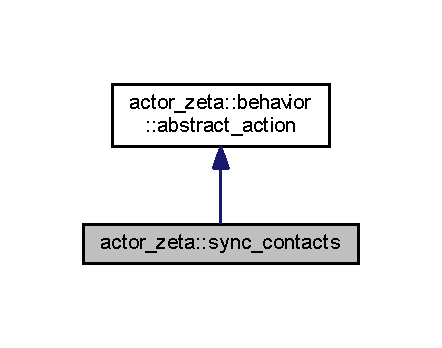
\includegraphics[width=212pt]{classactor__zeta_1_1sync__contacts__inherit__graph}
\end{center}
\end{figure}


Collaboration diagram for actor\+\_\+zeta\+:\+:sync\+\_\+contacts\+:\nopagebreak
\begin{figure}[H]
\begin{center}
\leavevmode
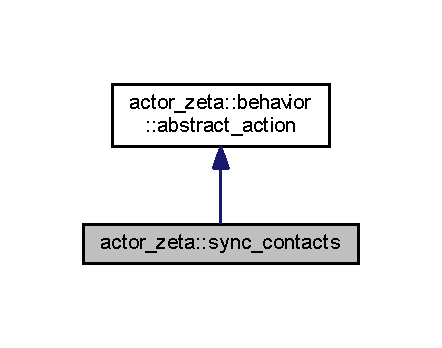
\includegraphics[width=212pt]{classactor__zeta_1_1sync__contacts__coll__graph}
\end{center}
\end{figure}
\subsection*{Public Member Functions}
\begin{DoxyCompactItemize}
\item 
\hyperlink{classactor__zeta_1_1sync__contacts_abd18e91a793caa6938a1384251e5180c}{sync\+\_\+contacts} ()
\item 
\hyperlink{classactor__zeta_1_1behavior_1_1response}{behavior\+::response} $\ast$ \hyperlink{classactor__zeta_1_1sync__contacts_ab135afb3284f42dc36d54ea73a8b5ac8}{operator()} (\hyperlink{classactor__zeta_1_1behavior_1_1request}{behavior\+::request} $\ast$) override final
\end{DoxyCompactItemize}


\subsection{Detailed Description}
A class used for contact operations synchronization. 

\subsection{Constructor \& Destructor Documentation}
\mbox{\Hypertarget{classactor__zeta_1_1sync__contacts_abd18e91a793caa6938a1384251e5180c}\label{classactor__zeta_1_1sync__contacts_abd18e91a793caa6938a1384251e5180c}} 
\index{actor\+\_\+zeta\+::sync\+\_\+contacts@{actor\+\_\+zeta\+::sync\+\_\+contacts}!sync\+\_\+contacts@{sync\+\_\+contacts}}
\index{sync\+\_\+contacts@{sync\+\_\+contacts}!actor\+\_\+zeta\+::sync\+\_\+contacts@{actor\+\_\+zeta\+::sync\+\_\+contacts}}
\subsubsection{\texorpdfstring{sync\+\_\+contacts()}{sync\_contacts()}}
{\footnotesize\ttfamily actor\+\_\+zeta\+::sync\+\_\+contacts\+::sync\+\_\+contacts (\begin{DoxyParamCaption}{ }\end{DoxyParamCaption})}



\subsection{Member Function Documentation}
\mbox{\Hypertarget{classactor__zeta_1_1sync__contacts_ab135afb3284f42dc36d54ea73a8b5ac8}\label{classactor__zeta_1_1sync__contacts_ab135afb3284f42dc36d54ea73a8b5ac8}} 
\index{actor\+\_\+zeta\+::sync\+\_\+contacts@{actor\+\_\+zeta\+::sync\+\_\+contacts}!operator()@{operator()}}
\index{operator()@{operator()}!actor\+\_\+zeta\+::sync\+\_\+contacts@{actor\+\_\+zeta\+::sync\+\_\+contacts}}
\subsubsection{\texorpdfstring{operator()()}{operator()()}}
{\footnotesize\ttfamily \hyperlink{classactor__zeta_1_1behavior_1_1response}{behavior\+::response} $\ast$ actor\+\_\+zeta\+::sync\+\_\+contacts\+::operator() (\begin{DoxyParamCaption}\item[{\hyperlink{classactor__zeta_1_1behavior_1_1request}{behavior\+::request} $\ast$}]{request }\end{DoxyParamCaption})\hspace{0.3cm}{\ttfamily [final]}, {\ttfamily [override]}, {\ttfamily [virtual]}}



Implements \hyperlink{classactor__zeta_1_1behavior_1_1abstract__action_a5e48075d77fbd93615fc9b757e6a4d87}{actor\+\_\+zeta\+::behavior\+::abstract\+\_\+action}.



The documentation for this class was generated from the following files\+:\begin{DoxyCompactItemize}
\item 
\hyperlink{sync__contacts_8hpp}{sync\+\_\+contacts.\+hpp}\item 
\hyperlink{sync__contacts_8cpp}{sync\+\_\+contacts.\+cpp}\end{DoxyCompactItemize}

\hypertarget{classactor__zeta_1_1behavior_1_1type__action}{}\section{actor\+\_\+zeta\+:\+:behavior\+:\+:type\+\_\+action Class Reference}
\label{classactor__zeta_1_1behavior_1_1type__action}\index{actor\+\_\+zeta\+::behavior\+::type\+\_\+action@{actor\+\_\+zeta\+::behavior\+::type\+\_\+action}}


Type of commands used for lyfecycle.  




{\ttfamily \#include $<$type\+\_\+action.\+hpp$>$}

\subsection*{Public Member Functions}
\begin{DoxyCompactItemize}
\item 
\hyperlink{classactor__zeta_1_1behavior_1_1type__action_a2684aef901ba95f08c26234dc5efde8c}{type\+\_\+action} ()=delete
\item 
\hyperlink{classactor__zeta_1_1behavior_1_1type__action_a463568dc753fb94928762d63a9e77bbe}{type\+\_\+action} (const \hyperlink{classactor__zeta_1_1behavior_1_1type__action}{type\+\_\+action} \&)=default
\item 
\hyperlink{classactor__zeta_1_1behavior_1_1type__action}{type\+\_\+action} \& \hyperlink{classactor__zeta_1_1behavior_1_1type__action_ac6d0744593acdee1755bf4c8647142e0}{operator=} (const \hyperlink{classactor__zeta_1_1behavior_1_1type__action}{type\+\_\+action} \&t)=default
\item 
\hyperlink{classactor__zeta_1_1behavior_1_1type__action_a09c272ebf6681a7abf16e96a40b00e68}{type\+\_\+action} (\hyperlink{classactor__zeta_1_1behavior_1_1type__action}{type\+\_\+action} \&\&)=default
\item 
\hyperlink{classactor__zeta_1_1behavior_1_1type__action}{type\+\_\+action} \& \hyperlink{classactor__zeta_1_1behavior_1_1type__action_a9c0705753fc6a12e1e264e58623669b5}{operator=} (\hyperlink{classactor__zeta_1_1behavior_1_1type__action}{type\+\_\+action} \&\&)=default
\item 
\hyperlink{classactor__zeta_1_1behavior_1_1type__action_a7ae1be97143d5d4b3c04dd4761ca56f9}{$\sim$type\+\_\+action} ()=default
\item 
{\footnotesize template$<$std\+::size\+\_\+t N$>$ }\\\hyperlink{classactor__zeta_1_1behavior_1_1type__action_a19d364a67100c9e9c6c4bd0619a23dcf}{type\+\_\+action} (const char(\&a\+Str)\mbox{[}N\mbox{]})
\item 
\hyperlink{classactor__zeta_1_1behavior_1_1type__action_a271663f992dbe82047cb37a742138376}{type\+\_\+action} (const char $\ast$, std\+::size\+\_\+t)
\item 
\hyperlink{classactor__zeta_1_1behavior_1_1type__action_a0406af5cd674a0ae8267764dfd3dc7c2}{type\+\_\+action} (const std\+::string \&)
\item 
bool \hyperlink{classactor__zeta_1_1behavior_1_1type__action_a852901cc2a9a35ede73535701e28eda2}{operator==} (const \hyperlink{classactor__zeta_1_1behavior_1_1type__action}{type\+\_\+action} \&t) const noexcept
\item 
auto \hyperlink{classactor__zeta_1_1behavior_1_1type__action_a60c1a881e40facb9390faed4b54ea5c7}{hash} () const noexcept -\/$>$ std\+::size\+\_\+t
\item 
auto \hyperlink{classactor__zeta_1_1behavior_1_1type__action_aea8bf387fe61053322c0862f0f7c7f09}{to\+\_\+string} () const -\/$>$ const std\+::string \&
\end{DoxyCompactItemize}


\subsection{Detailed Description}
Type of commands used for lyfecycle. 

\subsection{Constructor \& Destructor Documentation}
\mbox{\Hypertarget{classactor__zeta_1_1behavior_1_1type__action_a2684aef901ba95f08c26234dc5efde8c}\label{classactor__zeta_1_1behavior_1_1type__action_a2684aef901ba95f08c26234dc5efde8c}} 
\index{actor\+\_\+zeta\+::behavior\+::type\+\_\+action@{actor\+\_\+zeta\+::behavior\+::type\+\_\+action}!type\+\_\+action@{type\+\_\+action}}
\index{type\+\_\+action@{type\+\_\+action}!actor\+\_\+zeta\+::behavior\+::type\+\_\+action@{actor\+\_\+zeta\+::behavior\+::type\+\_\+action}}
\subsubsection{\texorpdfstring{type\+\_\+action()}{type\_action()}\hspace{0.1cm}{\footnotesize\ttfamily [1/6]}}
{\footnotesize\ttfamily actor\+\_\+zeta\+::behavior\+::type\+\_\+action\+::type\+\_\+action (\begin{DoxyParamCaption}{ }\end{DoxyParamCaption})\hspace{0.3cm}{\ttfamily [delete]}}

\mbox{\Hypertarget{classactor__zeta_1_1behavior_1_1type__action_a463568dc753fb94928762d63a9e77bbe}\label{classactor__zeta_1_1behavior_1_1type__action_a463568dc753fb94928762d63a9e77bbe}} 
\index{actor\+\_\+zeta\+::behavior\+::type\+\_\+action@{actor\+\_\+zeta\+::behavior\+::type\+\_\+action}!type\+\_\+action@{type\+\_\+action}}
\index{type\+\_\+action@{type\+\_\+action}!actor\+\_\+zeta\+::behavior\+::type\+\_\+action@{actor\+\_\+zeta\+::behavior\+::type\+\_\+action}}
\subsubsection{\texorpdfstring{type\+\_\+action()}{type\_action()}\hspace{0.1cm}{\footnotesize\ttfamily [2/6]}}
{\footnotesize\ttfamily actor\+\_\+zeta\+::behavior\+::type\+\_\+action\+::type\+\_\+action (\begin{DoxyParamCaption}\item[{const \hyperlink{classactor__zeta_1_1behavior_1_1type__action}{type\+\_\+action} \&}]{ }\end{DoxyParamCaption})\hspace{0.3cm}{\ttfamily [default]}}

\mbox{\Hypertarget{classactor__zeta_1_1behavior_1_1type__action_a09c272ebf6681a7abf16e96a40b00e68}\label{classactor__zeta_1_1behavior_1_1type__action_a09c272ebf6681a7abf16e96a40b00e68}} 
\index{actor\+\_\+zeta\+::behavior\+::type\+\_\+action@{actor\+\_\+zeta\+::behavior\+::type\+\_\+action}!type\+\_\+action@{type\+\_\+action}}
\index{type\+\_\+action@{type\+\_\+action}!actor\+\_\+zeta\+::behavior\+::type\+\_\+action@{actor\+\_\+zeta\+::behavior\+::type\+\_\+action}}
\subsubsection{\texorpdfstring{type\+\_\+action()}{type\_action()}\hspace{0.1cm}{\footnotesize\ttfamily [3/6]}}
{\footnotesize\ttfamily actor\+\_\+zeta\+::behavior\+::type\+\_\+action\+::type\+\_\+action (\begin{DoxyParamCaption}\item[{\hyperlink{classactor__zeta_1_1behavior_1_1type__action}{type\+\_\+action} \&\&}]{ }\end{DoxyParamCaption})\hspace{0.3cm}{\ttfamily [default]}}

\mbox{\Hypertarget{classactor__zeta_1_1behavior_1_1type__action_a7ae1be97143d5d4b3c04dd4761ca56f9}\label{classactor__zeta_1_1behavior_1_1type__action_a7ae1be97143d5d4b3c04dd4761ca56f9}} 
\index{actor\+\_\+zeta\+::behavior\+::type\+\_\+action@{actor\+\_\+zeta\+::behavior\+::type\+\_\+action}!````~type\+\_\+action@{$\sim$type\+\_\+action}}
\index{````~type\+\_\+action@{$\sim$type\+\_\+action}!actor\+\_\+zeta\+::behavior\+::type\+\_\+action@{actor\+\_\+zeta\+::behavior\+::type\+\_\+action}}
\subsubsection{\texorpdfstring{$\sim$type\+\_\+action()}{~type\_action()}}
{\footnotesize\ttfamily actor\+\_\+zeta\+::behavior\+::type\+\_\+action\+::$\sim$type\+\_\+action (\begin{DoxyParamCaption}{ }\end{DoxyParamCaption})\hspace{0.3cm}{\ttfamily [default]}}

\mbox{\Hypertarget{classactor__zeta_1_1behavior_1_1type__action_a19d364a67100c9e9c6c4bd0619a23dcf}\label{classactor__zeta_1_1behavior_1_1type__action_a19d364a67100c9e9c6c4bd0619a23dcf}} 
\index{actor\+\_\+zeta\+::behavior\+::type\+\_\+action@{actor\+\_\+zeta\+::behavior\+::type\+\_\+action}!type\+\_\+action@{type\+\_\+action}}
\index{type\+\_\+action@{type\+\_\+action}!actor\+\_\+zeta\+::behavior\+::type\+\_\+action@{actor\+\_\+zeta\+::behavior\+::type\+\_\+action}}
\subsubsection{\texorpdfstring{type\+\_\+action()}{type\_action()}\hspace{0.1cm}{\footnotesize\ttfamily [4/6]}}
{\footnotesize\ttfamily template$<$std\+::size\+\_\+t N$>$ \\
actor\+\_\+zeta\+::behavior\+::type\+\_\+action\+::type\+\_\+action (\begin{DoxyParamCaption}\item[{const char(\&)}]{a\+Str\mbox{[}\+N\mbox{]} }\end{DoxyParamCaption})\hspace{0.3cm}{\ttfamily [inline]}}

\mbox{\Hypertarget{classactor__zeta_1_1behavior_1_1type__action_a271663f992dbe82047cb37a742138376}\label{classactor__zeta_1_1behavior_1_1type__action_a271663f992dbe82047cb37a742138376}} 
\index{actor\+\_\+zeta\+::behavior\+::type\+\_\+action@{actor\+\_\+zeta\+::behavior\+::type\+\_\+action}!type\+\_\+action@{type\+\_\+action}}
\index{type\+\_\+action@{type\+\_\+action}!actor\+\_\+zeta\+::behavior\+::type\+\_\+action@{actor\+\_\+zeta\+::behavior\+::type\+\_\+action}}
\subsubsection{\texorpdfstring{type\+\_\+action()}{type\_action()}\hspace{0.1cm}{\footnotesize\ttfamily [5/6]}}
{\footnotesize\ttfamily actor\+\_\+zeta\+::behavior\+::type\+\_\+action\+::type\+\_\+action (\begin{DoxyParamCaption}\item[{const char $\ast$}]{str,  }\item[{std\+::size\+\_\+t}]{len }\end{DoxyParamCaption})}

\mbox{\Hypertarget{classactor__zeta_1_1behavior_1_1type__action_a0406af5cd674a0ae8267764dfd3dc7c2}\label{classactor__zeta_1_1behavior_1_1type__action_a0406af5cd674a0ae8267764dfd3dc7c2}} 
\index{actor\+\_\+zeta\+::behavior\+::type\+\_\+action@{actor\+\_\+zeta\+::behavior\+::type\+\_\+action}!type\+\_\+action@{type\+\_\+action}}
\index{type\+\_\+action@{type\+\_\+action}!actor\+\_\+zeta\+::behavior\+::type\+\_\+action@{actor\+\_\+zeta\+::behavior\+::type\+\_\+action}}
\subsubsection{\texorpdfstring{type\+\_\+action()}{type\_action()}\hspace{0.1cm}{\footnotesize\ttfamily [6/6]}}
{\footnotesize\ttfamily actor\+\_\+zeta\+::behavior\+::type\+\_\+action\+::type\+\_\+action (\begin{DoxyParamCaption}\item[{const std\+::string \&}]{token }\end{DoxyParamCaption})}



\subsection{Member Function Documentation}
\mbox{\Hypertarget{classactor__zeta_1_1behavior_1_1type__action_a60c1a881e40facb9390faed4b54ea5c7}\label{classactor__zeta_1_1behavior_1_1type__action_a60c1a881e40facb9390faed4b54ea5c7}} 
\index{actor\+\_\+zeta\+::behavior\+::type\+\_\+action@{actor\+\_\+zeta\+::behavior\+::type\+\_\+action}!hash@{hash}}
\index{hash@{hash}!actor\+\_\+zeta\+::behavior\+::type\+\_\+action@{actor\+\_\+zeta\+::behavior\+::type\+\_\+action}}
\subsubsection{\texorpdfstring{hash()}{hash()}}
{\footnotesize\ttfamily auto actor\+\_\+zeta\+::behavior\+::type\+\_\+action\+::hash (\begin{DoxyParamCaption}{ }\end{DoxyParamCaption}) const -\/$>$ std\+::size\+\_\+t\hspace{0.3cm}{\ttfamily [noexcept]}}

\mbox{\Hypertarget{classactor__zeta_1_1behavior_1_1type__action_ac6d0744593acdee1755bf4c8647142e0}\label{classactor__zeta_1_1behavior_1_1type__action_ac6d0744593acdee1755bf4c8647142e0}} 
\index{actor\+\_\+zeta\+::behavior\+::type\+\_\+action@{actor\+\_\+zeta\+::behavior\+::type\+\_\+action}!operator=@{operator=}}
\index{operator=@{operator=}!actor\+\_\+zeta\+::behavior\+::type\+\_\+action@{actor\+\_\+zeta\+::behavior\+::type\+\_\+action}}
\subsubsection{\texorpdfstring{operator=()}{operator=()}\hspace{0.1cm}{\footnotesize\ttfamily [1/2]}}
{\footnotesize\ttfamily \hyperlink{classactor__zeta_1_1behavior_1_1type__action}{type\+\_\+action}\& actor\+\_\+zeta\+::behavior\+::type\+\_\+action\+::operator= (\begin{DoxyParamCaption}\item[{const \hyperlink{classactor__zeta_1_1behavior_1_1type__action}{type\+\_\+action} \&}]{t }\end{DoxyParamCaption})\hspace{0.3cm}{\ttfamily [default]}}

\mbox{\Hypertarget{classactor__zeta_1_1behavior_1_1type__action_a9c0705753fc6a12e1e264e58623669b5}\label{classactor__zeta_1_1behavior_1_1type__action_a9c0705753fc6a12e1e264e58623669b5}} 
\index{actor\+\_\+zeta\+::behavior\+::type\+\_\+action@{actor\+\_\+zeta\+::behavior\+::type\+\_\+action}!operator=@{operator=}}
\index{operator=@{operator=}!actor\+\_\+zeta\+::behavior\+::type\+\_\+action@{actor\+\_\+zeta\+::behavior\+::type\+\_\+action}}
\subsubsection{\texorpdfstring{operator=()}{operator=()}\hspace{0.1cm}{\footnotesize\ttfamily [2/2]}}
{\footnotesize\ttfamily \hyperlink{classactor__zeta_1_1behavior_1_1type__action}{type\+\_\+action}\& actor\+\_\+zeta\+::behavior\+::type\+\_\+action\+::operator= (\begin{DoxyParamCaption}\item[{\hyperlink{classactor__zeta_1_1behavior_1_1type__action}{type\+\_\+action} \&\&}]{ }\end{DoxyParamCaption})\hspace{0.3cm}{\ttfamily [default]}}

\mbox{\Hypertarget{classactor__zeta_1_1behavior_1_1type__action_a852901cc2a9a35ede73535701e28eda2}\label{classactor__zeta_1_1behavior_1_1type__action_a852901cc2a9a35ede73535701e28eda2}} 
\index{actor\+\_\+zeta\+::behavior\+::type\+\_\+action@{actor\+\_\+zeta\+::behavior\+::type\+\_\+action}!operator==@{operator==}}
\index{operator==@{operator==}!actor\+\_\+zeta\+::behavior\+::type\+\_\+action@{actor\+\_\+zeta\+::behavior\+::type\+\_\+action}}
\subsubsection{\texorpdfstring{operator==()}{operator==()}}
{\footnotesize\ttfamily bool actor\+\_\+zeta\+::behavior\+::type\+\_\+action\+::operator== (\begin{DoxyParamCaption}\item[{const \hyperlink{classactor__zeta_1_1behavior_1_1type__action}{type\+\_\+action} \&}]{t }\end{DoxyParamCaption}) const\hspace{0.3cm}{\ttfamily [noexcept]}}

\mbox{\Hypertarget{classactor__zeta_1_1behavior_1_1type__action_aea8bf387fe61053322c0862f0f7c7f09}\label{classactor__zeta_1_1behavior_1_1type__action_aea8bf387fe61053322c0862f0f7c7f09}} 
\index{actor\+\_\+zeta\+::behavior\+::type\+\_\+action@{actor\+\_\+zeta\+::behavior\+::type\+\_\+action}!to\+\_\+string@{to\+\_\+string}}
\index{to\+\_\+string@{to\+\_\+string}!actor\+\_\+zeta\+::behavior\+::type\+\_\+action@{actor\+\_\+zeta\+::behavior\+::type\+\_\+action}}
\subsubsection{\texorpdfstring{to\+\_\+string()}{to\_string()}}
{\footnotesize\ttfamily auto actor\+\_\+zeta\+::behavior\+::type\+\_\+action\+::to\+\_\+string (\begin{DoxyParamCaption}{ }\end{DoxyParamCaption}) const -\/$>$ const std\+::string\&}



The documentation for this class was generated from the following files\+:\begin{DoxyCompactItemize}
\item 
\hyperlink{type__action_8hpp}{type\+\_\+action.\+hpp}\item 
\hyperlink{type__action_8cpp}{type\+\_\+action.\+cpp}\end{DoxyCompactItemize}

\hypertarget{classactor__zeta_1_1executor_1_1work__sharing}{}\section{actor\+\_\+zeta\+:\+:executor\+:\+:work\+\_\+sharing Class Reference}
\label{classactor__zeta_1_1executor_1_1work__sharing}\index{actor\+\_\+zeta\+::executor\+::work\+\_\+sharing@{actor\+\_\+zeta\+::executor\+::work\+\_\+sharing}}


Stands for work sharing approach.  




{\ttfamily \#include $<$work\+\_\+sharing.\+hpp$>$}

\subsection*{Classes}
\begin{DoxyCompactItemize}
\item 
struct \hyperlink{structactor__zeta_1_1executor_1_1work__sharing_1_1coordinator__data}{coordinator\+\_\+data}
\begin{DoxyCompactList}\small\item\em This structure is used as coordinator data keeper. \end{DoxyCompactList}\item 
struct \hyperlink{structactor__zeta_1_1executor_1_1work__sharing_1_1worker__data}{worker\+\_\+data}
\begin{DoxyCompactList}\small\item\em This structure is used as worker data keeper. \end{DoxyCompactList}\end{DoxyCompactItemize}
\subsection*{Public Types}
\begin{DoxyCompactItemize}
\item 
using \hyperlink{classactor__zeta_1_1executor_1_1work__sharing_a4ed160584612bb4abf7e23ace3590801}{queue\+\_\+type} = std\+::list$<$ \hyperlink{structactor__zeta_1_1executor_1_1executable}{executable} $\ast$ $>$
\end{DoxyCompactItemize}
\subsection*{Public Member Functions}
\begin{DoxyCompactItemize}
\item 
\hyperlink{classactor__zeta_1_1executor_1_1work__sharing_a9cdcd201ba45a67964c5f38c31ec7014}{$\sim$work\+\_\+sharing} ()
\item 
{\footnotesize template$<$class Coordinator $>$ }\\void \hyperlink{classactor__zeta_1_1executor_1_1work__sharing_a8b35723bd97f41af9a2a0b0e41a12134}{enqueue} (Coordinator $\ast$self, \hyperlink{structactor__zeta_1_1executor_1_1executable}{executable} $\ast$job)
\item 
{\footnotesize template$<$class Coordinator $>$ }\\void \hyperlink{classactor__zeta_1_1executor_1_1work__sharing_a6c9cc365c9d02574ac626d093eb4a221}{central\+\_\+enqueue} (Coordinator $\ast$self, \hyperlink{structactor__zeta_1_1executor_1_1executable}{executable} $\ast$job)
\item 
{\footnotesize template$<$class Worker $>$ }\\void \hyperlink{classactor__zeta_1_1executor_1_1work__sharing_a594aa82538f4ecdd9613cfdf07851c02}{external\+\_\+enqueue} (Worker $\ast$self, \hyperlink{structactor__zeta_1_1executor_1_1executable}{executable} $\ast$job)
\item 
{\footnotesize template$<$class Worker $>$ }\\void \hyperlink{classactor__zeta_1_1executor_1_1work__sharing_a033f2d355e87c707d6467b8c0c85e925}{internal\+\_\+enqueue} (Worker $\ast$self, \hyperlink{structactor__zeta_1_1executor_1_1executable}{executable} $\ast$job)
\item 
{\footnotesize template$<$class Worker $>$ }\\void \hyperlink{classactor__zeta_1_1executor_1_1work__sharing_a74e9c2f71b9a8365e0f0712d625f2279}{resume\+\_\+job\+\_\+later} (Worker $\ast$self, \hyperlink{structactor__zeta_1_1executor_1_1executable}{executable} $\ast$job)
\item 
{\footnotesize template$<$class Worker $>$ }\\\hyperlink{structactor__zeta_1_1executor_1_1executable}{executable} $\ast$ \hyperlink{classactor__zeta_1_1executor_1_1work__sharing_ad889ed60c2d52beef083d3854e87e40b}{dequeue} (Worker $\ast$self)
\item 
{\footnotesize template$<$class Coordinator , class Unary\+Function $>$ }\\void \hyperlink{classactor__zeta_1_1executor_1_1work__sharing_a65e0a47d49b1fcd434b09c39210b143c}{foreach\+\_\+central\+\_\+resumable} (Coordinator $\ast$self, Unary\+Function f)
\end{DoxyCompactItemize}


\subsection{Detailed Description}
Stands for work sharing approach. 

\subsection{Member Typedef Documentation}
\mbox{\Hypertarget{classactor__zeta_1_1executor_1_1work__sharing_a4ed160584612bb4abf7e23ace3590801}\label{classactor__zeta_1_1executor_1_1work__sharing_a4ed160584612bb4abf7e23ace3590801}} 
\index{actor\+\_\+zeta\+::executor\+::work\+\_\+sharing@{actor\+\_\+zeta\+::executor\+::work\+\_\+sharing}!queue\+\_\+type@{queue\+\_\+type}}
\index{queue\+\_\+type@{queue\+\_\+type}!actor\+\_\+zeta\+::executor\+::work\+\_\+sharing@{actor\+\_\+zeta\+::executor\+::work\+\_\+sharing}}
\subsubsection{\texorpdfstring{queue\+\_\+type}{queue\_type}}
{\footnotesize\ttfamily using \hyperlink{classactor__zeta_1_1executor_1_1work__sharing_a4ed160584612bb4abf7e23ace3590801}{actor\+\_\+zeta\+::executor\+::work\+\_\+sharing\+::queue\+\_\+type} =  std\+::list$<$\hyperlink{structactor__zeta_1_1executor_1_1executable}{executable} $\ast$$>$}



\subsection{Constructor \& Destructor Documentation}
\mbox{\Hypertarget{classactor__zeta_1_1executor_1_1work__sharing_a9cdcd201ba45a67964c5f38c31ec7014}\label{classactor__zeta_1_1executor_1_1work__sharing_a9cdcd201ba45a67964c5f38c31ec7014}} 
\index{actor\+\_\+zeta\+::executor\+::work\+\_\+sharing@{actor\+\_\+zeta\+::executor\+::work\+\_\+sharing}!````~work\+\_\+sharing@{$\sim$work\+\_\+sharing}}
\index{````~work\+\_\+sharing@{$\sim$work\+\_\+sharing}!actor\+\_\+zeta\+::executor\+::work\+\_\+sharing@{actor\+\_\+zeta\+::executor\+::work\+\_\+sharing}}
\subsubsection{\texorpdfstring{$\sim$work\+\_\+sharing()}{~work\_sharing()}}
{\footnotesize\ttfamily actor\+\_\+zeta\+::executor\+::work\+\_\+sharing\+::$\sim$work\+\_\+sharing (\begin{DoxyParamCaption}{ }\end{DoxyParamCaption})\hspace{0.3cm}{\ttfamily [inline]}}



\subsection{Member Function Documentation}
\mbox{\Hypertarget{classactor__zeta_1_1executor_1_1work__sharing_a6c9cc365c9d02574ac626d093eb4a221}\label{classactor__zeta_1_1executor_1_1work__sharing_a6c9cc365c9d02574ac626d093eb4a221}} 
\index{actor\+\_\+zeta\+::executor\+::work\+\_\+sharing@{actor\+\_\+zeta\+::executor\+::work\+\_\+sharing}!central\+\_\+enqueue@{central\+\_\+enqueue}}
\index{central\+\_\+enqueue@{central\+\_\+enqueue}!actor\+\_\+zeta\+::executor\+::work\+\_\+sharing@{actor\+\_\+zeta\+::executor\+::work\+\_\+sharing}}
\subsubsection{\texorpdfstring{central\+\_\+enqueue()}{central\_enqueue()}}
{\footnotesize\ttfamily template$<$class Coordinator $>$ \\
void actor\+\_\+zeta\+::executor\+::work\+\_\+sharing\+::central\+\_\+enqueue (\begin{DoxyParamCaption}\item[{Coordinator $\ast$}]{self,  }\item[{\hyperlink{structactor__zeta_1_1executor_1_1executable}{executable} $\ast$}]{job }\end{DoxyParamCaption})\hspace{0.3cm}{\ttfamily [inline]}}

\mbox{\Hypertarget{classactor__zeta_1_1executor_1_1work__sharing_ad889ed60c2d52beef083d3854e87e40b}\label{classactor__zeta_1_1executor_1_1work__sharing_ad889ed60c2d52beef083d3854e87e40b}} 
\index{actor\+\_\+zeta\+::executor\+::work\+\_\+sharing@{actor\+\_\+zeta\+::executor\+::work\+\_\+sharing}!dequeue@{dequeue}}
\index{dequeue@{dequeue}!actor\+\_\+zeta\+::executor\+::work\+\_\+sharing@{actor\+\_\+zeta\+::executor\+::work\+\_\+sharing}}
\subsubsection{\texorpdfstring{dequeue()}{dequeue()}}
{\footnotesize\ttfamily template$<$class Worker $>$ \\
\hyperlink{structactor__zeta_1_1executor_1_1executable}{executable}$\ast$ actor\+\_\+zeta\+::executor\+::work\+\_\+sharing\+::dequeue (\begin{DoxyParamCaption}\item[{Worker $\ast$}]{self }\end{DoxyParamCaption})\hspace{0.3cm}{\ttfamily [inline]}}

\mbox{\Hypertarget{classactor__zeta_1_1executor_1_1work__sharing_a8b35723bd97f41af9a2a0b0e41a12134}\label{classactor__zeta_1_1executor_1_1work__sharing_a8b35723bd97f41af9a2a0b0e41a12134}} 
\index{actor\+\_\+zeta\+::executor\+::work\+\_\+sharing@{actor\+\_\+zeta\+::executor\+::work\+\_\+sharing}!enqueue@{enqueue}}
\index{enqueue@{enqueue}!actor\+\_\+zeta\+::executor\+::work\+\_\+sharing@{actor\+\_\+zeta\+::executor\+::work\+\_\+sharing}}
\subsubsection{\texorpdfstring{enqueue()}{enqueue()}}
{\footnotesize\ttfamily template$<$class Coordinator $>$ \\
void actor\+\_\+zeta\+::executor\+::work\+\_\+sharing\+::enqueue (\begin{DoxyParamCaption}\item[{Coordinator $\ast$}]{self,  }\item[{\hyperlink{structactor__zeta_1_1executor_1_1executable}{executable} $\ast$}]{job }\end{DoxyParamCaption})\hspace{0.3cm}{\ttfamily [inline]}}

\mbox{\Hypertarget{classactor__zeta_1_1executor_1_1work__sharing_a594aa82538f4ecdd9613cfdf07851c02}\label{classactor__zeta_1_1executor_1_1work__sharing_a594aa82538f4ecdd9613cfdf07851c02}} 
\index{actor\+\_\+zeta\+::executor\+::work\+\_\+sharing@{actor\+\_\+zeta\+::executor\+::work\+\_\+sharing}!external\+\_\+enqueue@{external\+\_\+enqueue}}
\index{external\+\_\+enqueue@{external\+\_\+enqueue}!actor\+\_\+zeta\+::executor\+::work\+\_\+sharing@{actor\+\_\+zeta\+::executor\+::work\+\_\+sharing}}
\subsubsection{\texorpdfstring{external\+\_\+enqueue()}{external\_enqueue()}}
{\footnotesize\ttfamily template$<$class Worker $>$ \\
void actor\+\_\+zeta\+::executor\+::work\+\_\+sharing\+::external\+\_\+enqueue (\begin{DoxyParamCaption}\item[{Worker $\ast$}]{self,  }\item[{\hyperlink{structactor__zeta_1_1executor_1_1executable}{executable} $\ast$}]{job }\end{DoxyParamCaption})\hspace{0.3cm}{\ttfamily [inline]}}

\mbox{\Hypertarget{classactor__zeta_1_1executor_1_1work__sharing_a65e0a47d49b1fcd434b09c39210b143c}\label{classactor__zeta_1_1executor_1_1work__sharing_a65e0a47d49b1fcd434b09c39210b143c}} 
\index{actor\+\_\+zeta\+::executor\+::work\+\_\+sharing@{actor\+\_\+zeta\+::executor\+::work\+\_\+sharing}!foreach\+\_\+central\+\_\+resumable@{foreach\+\_\+central\+\_\+resumable}}
\index{foreach\+\_\+central\+\_\+resumable@{foreach\+\_\+central\+\_\+resumable}!actor\+\_\+zeta\+::executor\+::work\+\_\+sharing@{actor\+\_\+zeta\+::executor\+::work\+\_\+sharing}}
\subsubsection{\texorpdfstring{foreach\+\_\+central\+\_\+resumable()}{foreach\_central\_resumable()}}
{\footnotesize\ttfamily template$<$class Coordinator , class Unary\+Function $>$ \\
void actor\+\_\+zeta\+::executor\+::work\+\_\+sharing\+::foreach\+\_\+central\+\_\+resumable (\begin{DoxyParamCaption}\item[{Coordinator $\ast$}]{self,  }\item[{Unary\+Function}]{f }\end{DoxyParamCaption})\hspace{0.3cm}{\ttfamily [inline]}}

\mbox{\Hypertarget{classactor__zeta_1_1executor_1_1work__sharing_a033f2d355e87c707d6467b8c0c85e925}\label{classactor__zeta_1_1executor_1_1work__sharing_a033f2d355e87c707d6467b8c0c85e925}} 
\index{actor\+\_\+zeta\+::executor\+::work\+\_\+sharing@{actor\+\_\+zeta\+::executor\+::work\+\_\+sharing}!internal\+\_\+enqueue@{internal\+\_\+enqueue}}
\index{internal\+\_\+enqueue@{internal\+\_\+enqueue}!actor\+\_\+zeta\+::executor\+::work\+\_\+sharing@{actor\+\_\+zeta\+::executor\+::work\+\_\+sharing}}
\subsubsection{\texorpdfstring{internal\+\_\+enqueue()}{internal\_enqueue()}}
{\footnotesize\ttfamily template$<$class Worker $>$ \\
void actor\+\_\+zeta\+::executor\+::work\+\_\+sharing\+::internal\+\_\+enqueue (\begin{DoxyParamCaption}\item[{Worker $\ast$}]{self,  }\item[{\hyperlink{structactor__zeta_1_1executor_1_1executable}{executable} $\ast$}]{job }\end{DoxyParamCaption})\hspace{0.3cm}{\ttfamily [inline]}}

\mbox{\Hypertarget{classactor__zeta_1_1executor_1_1work__sharing_a74e9c2f71b9a8365e0f0712d625f2279}\label{classactor__zeta_1_1executor_1_1work__sharing_a74e9c2f71b9a8365e0f0712d625f2279}} 
\index{actor\+\_\+zeta\+::executor\+::work\+\_\+sharing@{actor\+\_\+zeta\+::executor\+::work\+\_\+sharing}!resume\+\_\+job\+\_\+later@{resume\+\_\+job\+\_\+later}}
\index{resume\+\_\+job\+\_\+later@{resume\+\_\+job\+\_\+later}!actor\+\_\+zeta\+::executor\+::work\+\_\+sharing@{actor\+\_\+zeta\+::executor\+::work\+\_\+sharing}}
\subsubsection{\texorpdfstring{resume\+\_\+job\+\_\+later()}{resume\_job\_later()}}
{\footnotesize\ttfamily template$<$class Worker $>$ \\
void actor\+\_\+zeta\+::executor\+::work\+\_\+sharing\+::resume\+\_\+job\+\_\+later (\begin{DoxyParamCaption}\item[{Worker $\ast$}]{self,  }\item[{\hyperlink{structactor__zeta_1_1executor_1_1executable}{executable} $\ast$}]{job }\end{DoxyParamCaption})\hspace{0.3cm}{\ttfamily [inline]}}



The documentation for this class was generated from the following file\+:\begin{DoxyCompactItemize}
\item 
\hyperlink{work__sharing_8hpp}{work\+\_\+sharing.\+hpp}\end{DoxyCompactItemize}

\hypertarget{classactor__zeta_1_1executor_1_1worker}{}\section{actor\+\_\+zeta\+:\+:executor\+:\+:worker$<$ Policy $>$ Class Template Reference}
\label{classactor__zeta_1_1executor_1_1worker}\index{actor\+\_\+zeta\+::executor\+::worker$<$ Policy $>$@{actor\+\_\+zeta\+::executor\+::worker$<$ Policy $>$}}


A simple worker module class.  




{\ttfamily \#include $<$worker.\+hpp$>$}



Inheritance diagram for actor\+\_\+zeta\+:\+:executor\+:\+:worker$<$ Policy $>$\+:\nopagebreak
\begin{figure}[H]
\begin{center}
\leavevmode
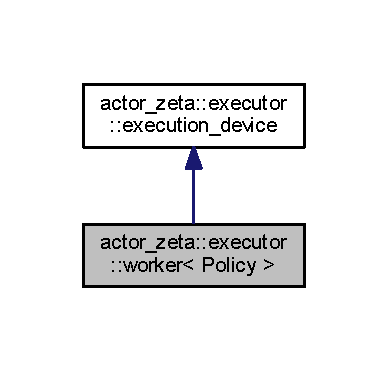
\includegraphics[width=186pt]{classactor__zeta_1_1executor_1_1worker__inherit__graph}
\end{center}
\end{figure}


Collaboration diagram for actor\+\_\+zeta\+:\+:executor\+:\+:worker$<$ Policy $>$\+:\nopagebreak
\begin{figure}[H]
\begin{center}
\leavevmode
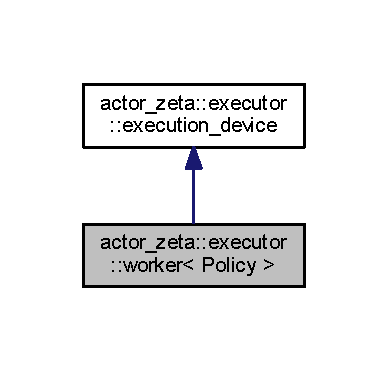
\includegraphics[width=186pt]{classactor__zeta_1_1executor_1_1worker__coll__graph}
\end{center}
\end{figure}
\subsection*{Public Types}
\begin{DoxyCompactItemize}
\item 
using \hyperlink{classactor__zeta_1_1executor_1_1worker_a74e3d9df71ad0b0df8d0c5403f8e642a}{job\+\_\+ptr} = \hyperlink{structactor__zeta_1_1executor_1_1executable}{executable} $\ast$
\item 
using \hyperlink{classactor__zeta_1_1executor_1_1worker_a0f64bbb63577325b5217ccee17a28738}{coordinator\+\_\+ptr} = \hyperlink{classactor__zeta_1_1executor_1_1coordinator}{coordinator}$<$ Policy $>$ $\ast$
\item 
using \hyperlink{classactor__zeta_1_1executor_1_1worker_ad8f39b0132441963ede8c1e8435aebb2}{policy\+\_\+data} = typename Policy\+::worker\+\_\+data
\end{DoxyCompactItemize}
\subsection*{Public Member Functions}
\begin{DoxyCompactItemize}
\item 
\hyperlink{classactor__zeta_1_1executor_1_1worker_a674d91050c8ae364156501f9abb7ecd3}{worker} (size\+\_\+t worker\+\_\+id, \hyperlink{classactor__zeta_1_1executor_1_1worker_a0f64bbb63577325b5217ccee17a28738}{coordinator\+\_\+ptr} worker\+\_\+parent, size\+\_\+t throughput)
\item 
void \hyperlink{classactor__zeta_1_1executor_1_1worker_a257ad22771ecbf3a9dbb1b2e86106893}{start} ()
\item 
\hyperlink{classactor__zeta_1_1executor_1_1worker_a67c327dc2d357864799117c8358a736e}{worker} (const \hyperlink{classactor__zeta_1_1executor_1_1worker}{worker} \&)=delete
\item 
\hyperlink{classactor__zeta_1_1executor_1_1worker}{worker} \& \hyperlink{classactor__zeta_1_1executor_1_1worker_a5ee4aa24cacffc8f620ea0094b4dbada}{operator=} (const \hyperlink{classactor__zeta_1_1executor_1_1worker}{worker} \&)=delete
\item 
void \hyperlink{classactor__zeta_1_1executor_1_1worker_acd3696b6425009eee551db3bb34b800f}{external\+\_\+enqueue} (\hyperlink{classactor__zeta_1_1executor_1_1worker_a74e3d9df71ad0b0df8d0c5403f8e642a}{job\+\_\+ptr} job)
\item 
void \hyperlink{classactor__zeta_1_1executor_1_1worker_a64480cdfc253eddf75ff0798928163c6}{put\+\_\+execute\+\_\+latest} (\hyperlink{classactor__zeta_1_1executor_1_1worker_a74e3d9df71ad0b0df8d0c5403f8e642a}{job\+\_\+ptr} job) override
\item 
\hyperlink{classactor__zeta_1_1executor_1_1worker_a0f64bbb63577325b5217ccee17a28738}{coordinator\+\_\+ptr} \hyperlink{classactor__zeta_1_1executor_1_1worker_aa3f0840f8fa873ff6300e72cbf753cfd}{parent} ()
\item 
size\+\_\+t \hyperlink{classactor__zeta_1_1executor_1_1worker_a0d3f8ce9e97f2fb78e6e0b213b620eb8}{id} () const
\item 
\hyperlink{classactor__zeta_1_1executor_1_1worker_ad8f39b0132441963ede8c1e8435aebb2}{policy\+\_\+data} \& \hyperlink{classactor__zeta_1_1executor_1_1worker_a2b687c0dde52737dd2c4701117d6abb1}{data} ()
\item 
size\+\_\+t \hyperlink{classactor__zeta_1_1executor_1_1worker_a1bfce28f14af95a760912ebc12112305}{max\+\_\+throughput} ()
\end{DoxyCompactItemize}


\subsection{Detailed Description}
\subsubsection*{template$<$class Policy$>$\newline
class actor\+\_\+zeta\+::executor\+::worker$<$ Policy $>$}

A simple worker module class. 


\begin{DoxyTemplParams}{Template Parameters}
{\em Policy} & \\
\hline
\end{DoxyTemplParams}


\subsection{Member Typedef Documentation}
\mbox{\Hypertarget{classactor__zeta_1_1executor_1_1worker_a0f64bbb63577325b5217ccee17a28738}\label{classactor__zeta_1_1executor_1_1worker_a0f64bbb63577325b5217ccee17a28738}} 
\index{actor\+\_\+zeta\+::executor\+::worker@{actor\+\_\+zeta\+::executor\+::worker}!coordinator\+\_\+ptr@{coordinator\+\_\+ptr}}
\index{coordinator\+\_\+ptr@{coordinator\+\_\+ptr}!actor\+\_\+zeta\+::executor\+::worker@{actor\+\_\+zeta\+::executor\+::worker}}
\subsubsection{\texorpdfstring{coordinator\+\_\+ptr}{coordinator\_ptr}}
{\footnotesize\ttfamily template$<$class Policy $>$ \\
using \hyperlink{classactor__zeta_1_1executor_1_1worker}{actor\+\_\+zeta\+::executor\+::worker}$<$ Policy $>$\+::\hyperlink{classactor__zeta_1_1executor_1_1worker_a0f64bbb63577325b5217ccee17a28738}{coordinator\+\_\+ptr} =  \hyperlink{classactor__zeta_1_1executor_1_1coordinator}{coordinator}$<$Policy$>$ $\ast$}

\mbox{\Hypertarget{classactor__zeta_1_1executor_1_1worker_a74e3d9df71ad0b0df8d0c5403f8e642a}\label{classactor__zeta_1_1executor_1_1worker_a74e3d9df71ad0b0df8d0c5403f8e642a}} 
\index{actor\+\_\+zeta\+::executor\+::worker@{actor\+\_\+zeta\+::executor\+::worker}!job\+\_\+ptr@{job\+\_\+ptr}}
\index{job\+\_\+ptr@{job\+\_\+ptr}!actor\+\_\+zeta\+::executor\+::worker@{actor\+\_\+zeta\+::executor\+::worker}}
\subsubsection{\texorpdfstring{job\+\_\+ptr}{job\_ptr}}
{\footnotesize\ttfamily template$<$class Policy $>$ \\
using \hyperlink{classactor__zeta_1_1executor_1_1worker}{actor\+\_\+zeta\+::executor\+::worker}$<$ Policy $>$\+::\hyperlink{classactor__zeta_1_1executor_1_1worker_a74e3d9df71ad0b0df8d0c5403f8e642a}{job\+\_\+ptr} =  \hyperlink{structactor__zeta_1_1executor_1_1executable}{executable} $\ast$}

\mbox{\Hypertarget{classactor__zeta_1_1executor_1_1worker_ad8f39b0132441963ede8c1e8435aebb2}\label{classactor__zeta_1_1executor_1_1worker_ad8f39b0132441963ede8c1e8435aebb2}} 
\index{actor\+\_\+zeta\+::executor\+::worker@{actor\+\_\+zeta\+::executor\+::worker}!policy\+\_\+data@{policy\+\_\+data}}
\index{policy\+\_\+data@{policy\+\_\+data}!actor\+\_\+zeta\+::executor\+::worker@{actor\+\_\+zeta\+::executor\+::worker}}
\subsubsection{\texorpdfstring{policy\+\_\+data}{policy\_data}}
{\footnotesize\ttfamily template$<$class Policy $>$ \\
using \hyperlink{classactor__zeta_1_1executor_1_1worker}{actor\+\_\+zeta\+::executor\+::worker}$<$ Policy $>$\+::\hyperlink{classactor__zeta_1_1executor_1_1worker_ad8f39b0132441963ede8c1e8435aebb2}{policy\+\_\+data} =  typename Policy\+::worker\+\_\+data}



\subsection{Constructor \& Destructor Documentation}
\mbox{\Hypertarget{classactor__zeta_1_1executor_1_1worker_a674d91050c8ae364156501f9abb7ecd3}\label{classactor__zeta_1_1executor_1_1worker_a674d91050c8ae364156501f9abb7ecd3}} 
\index{actor\+\_\+zeta\+::executor\+::worker@{actor\+\_\+zeta\+::executor\+::worker}!worker@{worker}}
\index{worker@{worker}!actor\+\_\+zeta\+::executor\+::worker@{actor\+\_\+zeta\+::executor\+::worker}}
\subsubsection{\texorpdfstring{worker()}{worker()}\hspace{0.1cm}{\footnotesize\ttfamily [1/2]}}
{\footnotesize\ttfamily template$<$class Policy $>$ \\
\hyperlink{classactor__zeta_1_1executor_1_1worker}{actor\+\_\+zeta\+::executor\+::worker}$<$ Policy $>$\+::\hyperlink{classactor__zeta_1_1executor_1_1worker}{worker} (\begin{DoxyParamCaption}\item[{size\+\_\+t}]{worker\+\_\+id,  }\item[{\hyperlink{classactor__zeta_1_1executor_1_1worker_a0f64bbb63577325b5217ccee17a28738}{coordinator\+\_\+ptr}}]{worker\+\_\+parent,  }\item[{size\+\_\+t}]{throughput }\end{DoxyParamCaption})\hspace{0.3cm}{\ttfamily [inline]}}

\mbox{\Hypertarget{classactor__zeta_1_1executor_1_1worker_a67c327dc2d357864799117c8358a736e}\label{classactor__zeta_1_1executor_1_1worker_a67c327dc2d357864799117c8358a736e}} 
\index{actor\+\_\+zeta\+::executor\+::worker@{actor\+\_\+zeta\+::executor\+::worker}!worker@{worker}}
\index{worker@{worker}!actor\+\_\+zeta\+::executor\+::worker@{actor\+\_\+zeta\+::executor\+::worker}}
\subsubsection{\texorpdfstring{worker()}{worker()}\hspace{0.1cm}{\footnotesize\ttfamily [2/2]}}
{\footnotesize\ttfamily template$<$class Policy $>$ \\
\hyperlink{classactor__zeta_1_1executor_1_1worker}{actor\+\_\+zeta\+::executor\+::worker}$<$ Policy $>$\+::\hyperlink{classactor__zeta_1_1executor_1_1worker}{worker} (\begin{DoxyParamCaption}\item[{const \hyperlink{classactor__zeta_1_1executor_1_1worker}{worker}$<$ Policy $>$ \&}]{ }\end{DoxyParamCaption})\hspace{0.3cm}{\ttfamily [delete]}}



\subsection{Member Function Documentation}
\mbox{\Hypertarget{classactor__zeta_1_1executor_1_1worker_a2b687c0dde52737dd2c4701117d6abb1}\label{classactor__zeta_1_1executor_1_1worker_a2b687c0dde52737dd2c4701117d6abb1}} 
\index{actor\+\_\+zeta\+::executor\+::worker@{actor\+\_\+zeta\+::executor\+::worker}!data@{data}}
\index{data@{data}!actor\+\_\+zeta\+::executor\+::worker@{actor\+\_\+zeta\+::executor\+::worker}}
\subsubsection{\texorpdfstring{data()}{data()}}
{\footnotesize\ttfamily template$<$class Policy $>$ \\
\hyperlink{classactor__zeta_1_1executor_1_1worker_ad8f39b0132441963ede8c1e8435aebb2}{policy\+\_\+data}\& \hyperlink{classactor__zeta_1_1executor_1_1worker}{actor\+\_\+zeta\+::executor\+::worker}$<$ Policy $>$\+::data (\begin{DoxyParamCaption}{ }\end{DoxyParamCaption})\hspace{0.3cm}{\ttfamily [inline]}}

\mbox{\Hypertarget{classactor__zeta_1_1executor_1_1worker_acd3696b6425009eee551db3bb34b800f}\label{classactor__zeta_1_1executor_1_1worker_acd3696b6425009eee551db3bb34b800f}} 
\index{actor\+\_\+zeta\+::executor\+::worker@{actor\+\_\+zeta\+::executor\+::worker}!external\+\_\+enqueue@{external\+\_\+enqueue}}
\index{external\+\_\+enqueue@{external\+\_\+enqueue}!actor\+\_\+zeta\+::executor\+::worker@{actor\+\_\+zeta\+::executor\+::worker}}
\subsubsection{\texorpdfstring{external\+\_\+enqueue()}{external\_enqueue()}}
{\footnotesize\ttfamily template$<$class Policy $>$ \\
void \hyperlink{classactor__zeta_1_1executor_1_1worker}{actor\+\_\+zeta\+::executor\+::worker}$<$ Policy $>$\+::external\+\_\+enqueue (\begin{DoxyParamCaption}\item[{\hyperlink{classactor__zeta_1_1executor_1_1worker_a74e3d9df71ad0b0df8d0c5403f8e642a}{job\+\_\+ptr}}]{job }\end{DoxyParamCaption})\hspace{0.3cm}{\ttfamily [inline]}}

\mbox{\Hypertarget{classactor__zeta_1_1executor_1_1worker_a0d3f8ce9e97f2fb78e6e0b213b620eb8}\label{classactor__zeta_1_1executor_1_1worker_a0d3f8ce9e97f2fb78e6e0b213b620eb8}} 
\index{actor\+\_\+zeta\+::executor\+::worker@{actor\+\_\+zeta\+::executor\+::worker}!id@{id}}
\index{id@{id}!actor\+\_\+zeta\+::executor\+::worker@{actor\+\_\+zeta\+::executor\+::worker}}
\subsubsection{\texorpdfstring{id()}{id()}}
{\footnotesize\ttfamily template$<$class Policy $>$ \\
size\+\_\+t \hyperlink{classactor__zeta_1_1executor_1_1worker}{actor\+\_\+zeta\+::executor\+::worker}$<$ Policy $>$\+::id (\begin{DoxyParamCaption}{ }\end{DoxyParamCaption}) const\hspace{0.3cm}{\ttfamily [inline]}}

\mbox{\Hypertarget{classactor__zeta_1_1executor_1_1worker_a1bfce28f14af95a760912ebc12112305}\label{classactor__zeta_1_1executor_1_1worker_a1bfce28f14af95a760912ebc12112305}} 
\index{actor\+\_\+zeta\+::executor\+::worker@{actor\+\_\+zeta\+::executor\+::worker}!max\+\_\+throughput@{max\+\_\+throughput}}
\index{max\+\_\+throughput@{max\+\_\+throughput}!actor\+\_\+zeta\+::executor\+::worker@{actor\+\_\+zeta\+::executor\+::worker}}
\subsubsection{\texorpdfstring{max\+\_\+throughput()}{max\_throughput()}}
{\footnotesize\ttfamily template$<$class Policy $>$ \\
size\+\_\+t \hyperlink{classactor__zeta_1_1executor_1_1worker}{actor\+\_\+zeta\+::executor\+::worker}$<$ Policy $>$\+::max\+\_\+throughput (\begin{DoxyParamCaption}{ }\end{DoxyParamCaption})\hspace{0.3cm}{\ttfamily [inline]}}

\mbox{\Hypertarget{classactor__zeta_1_1executor_1_1worker_a5ee4aa24cacffc8f620ea0094b4dbada}\label{classactor__zeta_1_1executor_1_1worker_a5ee4aa24cacffc8f620ea0094b4dbada}} 
\index{actor\+\_\+zeta\+::executor\+::worker@{actor\+\_\+zeta\+::executor\+::worker}!operator=@{operator=}}
\index{operator=@{operator=}!actor\+\_\+zeta\+::executor\+::worker@{actor\+\_\+zeta\+::executor\+::worker}}
\subsubsection{\texorpdfstring{operator=()}{operator=()}}
{\footnotesize\ttfamily template$<$class Policy $>$ \\
\hyperlink{classactor__zeta_1_1executor_1_1worker}{worker}\& \hyperlink{classactor__zeta_1_1executor_1_1worker}{actor\+\_\+zeta\+::executor\+::worker}$<$ Policy $>$\+::operator= (\begin{DoxyParamCaption}\item[{const \hyperlink{classactor__zeta_1_1executor_1_1worker}{worker}$<$ Policy $>$ \&}]{ }\end{DoxyParamCaption})\hspace{0.3cm}{\ttfamily [delete]}}

\mbox{\Hypertarget{classactor__zeta_1_1executor_1_1worker_aa3f0840f8fa873ff6300e72cbf753cfd}\label{classactor__zeta_1_1executor_1_1worker_aa3f0840f8fa873ff6300e72cbf753cfd}} 
\index{actor\+\_\+zeta\+::executor\+::worker@{actor\+\_\+zeta\+::executor\+::worker}!parent@{parent}}
\index{parent@{parent}!actor\+\_\+zeta\+::executor\+::worker@{actor\+\_\+zeta\+::executor\+::worker}}
\subsubsection{\texorpdfstring{parent()}{parent()}}
{\footnotesize\ttfamily template$<$class Policy $>$ \\
\hyperlink{classactor__zeta_1_1executor_1_1worker_a0f64bbb63577325b5217ccee17a28738}{coordinator\+\_\+ptr} \hyperlink{classactor__zeta_1_1executor_1_1worker}{actor\+\_\+zeta\+::executor\+::worker}$<$ Policy $>$\+::parent (\begin{DoxyParamCaption}{ }\end{DoxyParamCaption})\hspace{0.3cm}{\ttfamily [inline]}}

\mbox{\Hypertarget{classactor__zeta_1_1executor_1_1worker_a64480cdfc253eddf75ff0798928163c6}\label{classactor__zeta_1_1executor_1_1worker_a64480cdfc253eddf75ff0798928163c6}} 
\index{actor\+\_\+zeta\+::executor\+::worker@{actor\+\_\+zeta\+::executor\+::worker}!put\+\_\+execute\+\_\+latest@{put\+\_\+execute\+\_\+latest}}
\index{put\+\_\+execute\+\_\+latest@{put\+\_\+execute\+\_\+latest}!actor\+\_\+zeta\+::executor\+::worker@{actor\+\_\+zeta\+::executor\+::worker}}
\subsubsection{\texorpdfstring{put\+\_\+execute\+\_\+latest()}{put\_execute\_latest()}}
{\footnotesize\ttfamily template$<$class Policy $>$ \\
void \hyperlink{classactor__zeta_1_1executor_1_1worker}{actor\+\_\+zeta\+::executor\+::worker}$<$ Policy $>$\+::put\+\_\+execute\+\_\+latest (\begin{DoxyParamCaption}\item[{\hyperlink{classactor__zeta_1_1executor_1_1worker_a74e3d9df71ad0b0df8d0c5403f8e642a}{job\+\_\+ptr}}]{job }\end{DoxyParamCaption})\hspace{0.3cm}{\ttfamily [inline]}, {\ttfamily [override]}}

\mbox{\Hypertarget{classactor__zeta_1_1executor_1_1worker_a257ad22771ecbf3a9dbb1b2e86106893}\label{classactor__zeta_1_1executor_1_1worker_a257ad22771ecbf3a9dbb1b2e86106893}} 
\index{actor\+\_\+zeta\+::executor\+::worker@{actor\+\_\+zeta\+::executor\+::worker}!start@{start}}
\index{start@{start}!actor\+\_\+zeta\+::executor\+::worker@{actor\+\_\+zeta\+::executor\+::worker}}
\subsubsection{\texorpdfstring{start()}{start()}}
{\footnotesize\ttfamily template$<$class Policy $>$ \\
void \hyperlink{classactor__zeta_1_1executor_1_1worker}{actor\+\_\+zeta\+::executor\+::worker}$<$ Policy $>$\+::start (\begin{DoxyParamCaption}{ }\end{DoxyParamCaption})\hspace{0.3cm}{\ttfamily [inline]}}



The documentation for this class was generated from the following file\+:\begin{DoxyCompactItemize}
\item 
\hyperlink{worker_8hpp}{worker.\+hpp}\end{DoxyCompactItemize}

\hypertarget{structactor__zeta_1_1executor_1_1work__sharing_1_1worker__data}{}\section{actor\+\_\+zeta\+:\+:executor\+:\+:work\+\_\+sharing\+:\+:worker\+\_\+data Struct Reference}
\label{structactor__zeta_1_1executor_1_1work__sharing_1_1worker__data}\index{actor\+\_\+zeta\+::executor\+::work\+\_\+sharing\+::worker\+\_\+data@{actor\+\_\+zeta\+::executor\+::work\+\_\+sharing\+::worker\+\_\+data}}


This structure is used as worker data keeper.  




{\ttfamily \#include $<$work\+\_\+sharing.\+hpp$>$}

\subsection*{Public Member Functions}
\begin{DoxyCompactItemize}
\item 
\hyperlink{structactor__zeta_1_1executor_1_1work__sharing_1_1worker__data_ae810eed60fd71ef938993dbafb50d41d}{worker\+\_\+data} (\hyperlink{classactor__zeta_1_1executor_1_1abstract__coordinator}{executor\+::abstract\+\_\+coordinator} $\ast$)
\end{DoxyCompactItemize}


\subsection{Detailed Description}
This structure is used as worker data keeper. 

\subsection{Constructor \& Destructor Documentation}
\mbox{\Hypertarget{structactor__zeta_1_1executor_1_1work__sharing_1_1worker__data_ae810eed60fd71ef938993dbafb50d41d}\label{structactor__zeta_1_1executor_1_1work__sharing_1_1worker__data_ae810eed60fd71ef938993dbafb50d41d}} 
\index{actor\+\_\+zeta\+::executor\+::work\+\_\+sharing\+::worker\+\_\+data@{actor\+\_\+zeta\+::executor\+::work\+\_\+sharing\+::worker\+\_\+data}!worker\+\_\+data@{worker\+\_\+data}}
\index{worker\+\_\+data@{worker\+\_\+data}!actor\+\_\+zeta\+::executor\+::work\+\_\+sharing\+::worker\+\_\+data@{actor\+\_\+zeta\+::executor\+::work\+\_\+sharing\+::worker\+\_\+data}}
\subsubsection{\texorpdfstring{worker\+\_\+data()}{worker\_data()}}
{\footnotesize\ttfamily actor\+\_\+zeta\+::executor\+::work\+\_\+sharing\+::worker\+\_\+data\+::worker\+\_\+data (\begin{DoxyParamCaption}\item[{\hyperlink{classactor__zeta_1_1executor_1_1abstract__coordinator}{executor\+::abstract\+\_\+coordinator} $\ast$}]{ }\end{DoxyParamCaption})\hspace{0.3cm}{\ttfamily [inline]}, {\ttfamily [explicit]}}



The documentation for this struct was generated from the following file\+:\begin{DoxyCompactItemize}
\item 
\hyperlink{work__sharing_8hpp}{work\+\_\+sharing.\+hpp}\end{DoxyCompactItemize}

\chapter{File Documentation}
\hypertarget{abstract__action_8hpp}{}\section{abstract\+\_\+action.\+hpp File Reference}
\label{abstract__action_8hpp}\index{abstract\+\_\+action.\+hpp@{abstract\+\_\+action.\+hpp}}
{\ttfamily \#include \char`\"{}actor-\/zeta/forwards.\+hpp\char`\"{}}\newline
{\ttfamily \#include \char`\"{}type\+\_\+action.\+hpp\char`\"{}}\newline
Include dependency graph for abstract\+\_\+action.\+hpp\+:\nopagebreak
\begin{figure}[H]
\begin{center}
\leavevmode
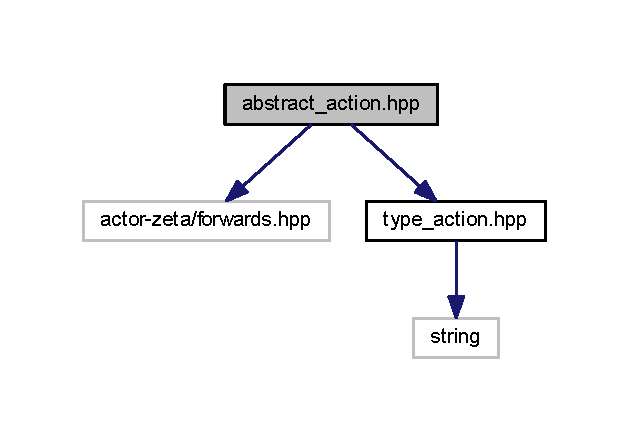
\includegraphics[width=302pt]{abstract__action_8hpp__incl}
\end{center}
\end{figure}
This graph shows which files directly or indirectly include this file\+:\nopagebreak
\begin{figure}[H]
\begin{center}
\leavevmode
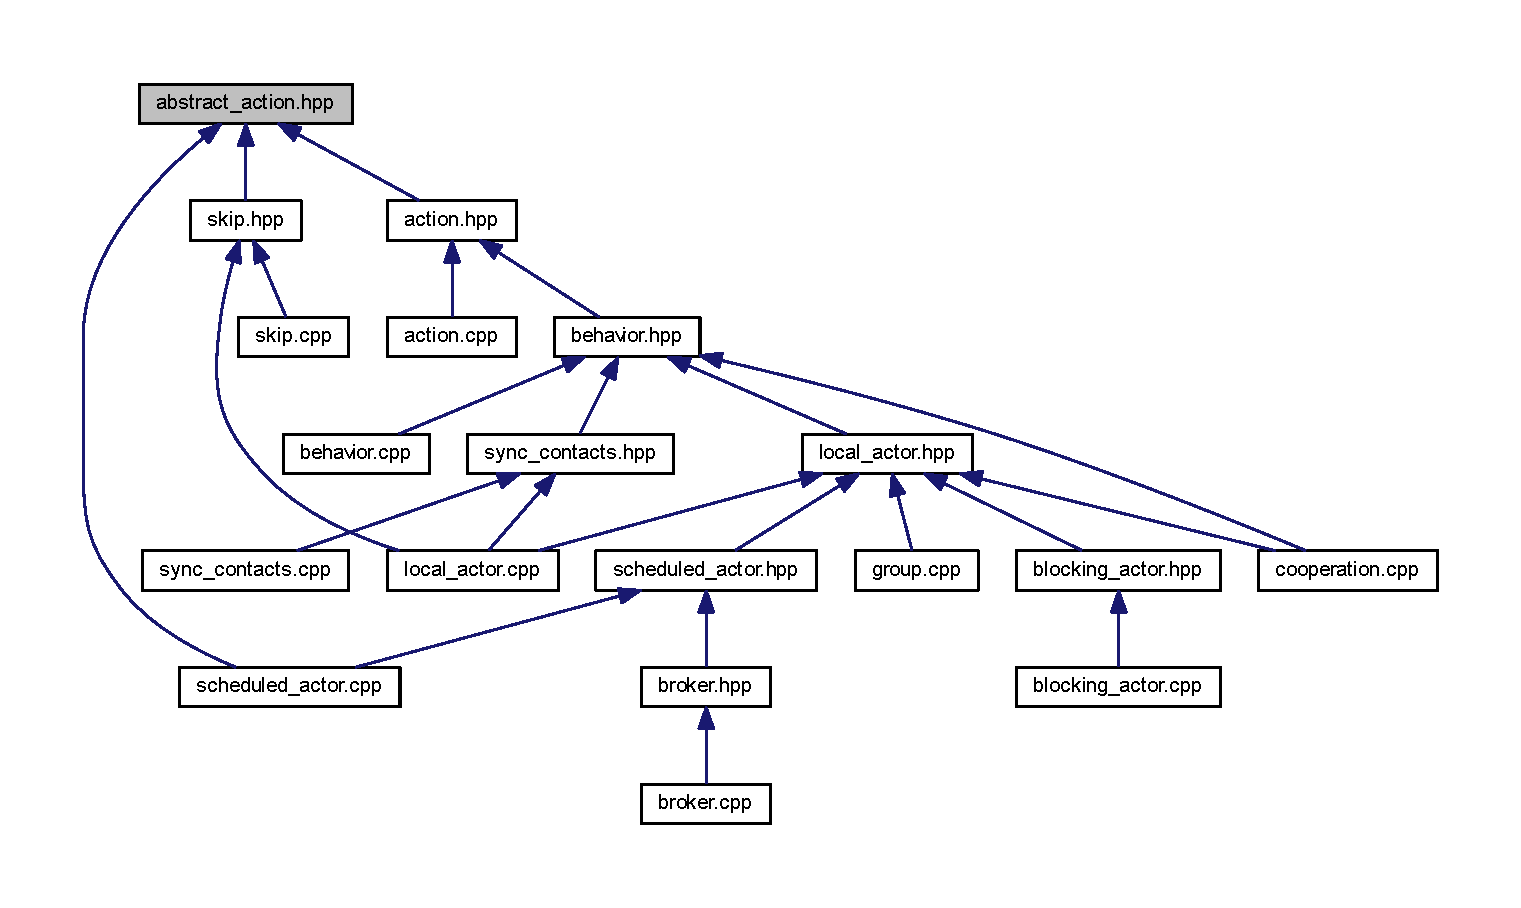
\includegraphics[width=350pt]{abstract__action_8hpp__dep__incl}
\end{center}
\end{figure}
\subsection*{Classes}
\begin{DoxyCompactItemize}
\item 
class \hyperlink{classactor__zeta_1_1behavior_1_1abstract__action}{actor\+\_\+zeta\+::behavior\+::abstract\+\_\+action}
\begin{DoxyCompactList}\small\item\em abstract concept of an action \end{DoxyCompactList}\end{DoxyCompactItemize}
\subsection*{Namespaces}
\begin{DoxyCompactItemize}
\item 
 \hyperlink{namespaceactor__zeta}{actor\+\_\+zeta}
\item 
 \hyperlink{namespaceactor__zeta_1_1behavior}{actor\+\_\+zeta\+::behavior}
\end{DoxyCompactItemize}

\hypertarget{abstract__actor_8cpp}{}\section{abstract\+\_\+actor.\+cpp File Reference}
\label{abstract__actor_8cpp}\index{abstract\+\_\+actor.\+cpp@{abstract\+\_\+actor.\+cpp}}
{\ttfamily \#include \char`\"{}actor-\/zeta/actor/abstract\+\_\+actor.\+hpp\char`\"{}}\newline
{\ttfamily \#include \char`\"{}actor-\/zeta/actor/actor\+\_\+address.\+hpp\char`\"{}}\newline
Include dependency graph for abstract\+\_\+actor.\+cpp\+:\nopagebreak
\begin{figure}[H]
\begin{center}
\leavevmode
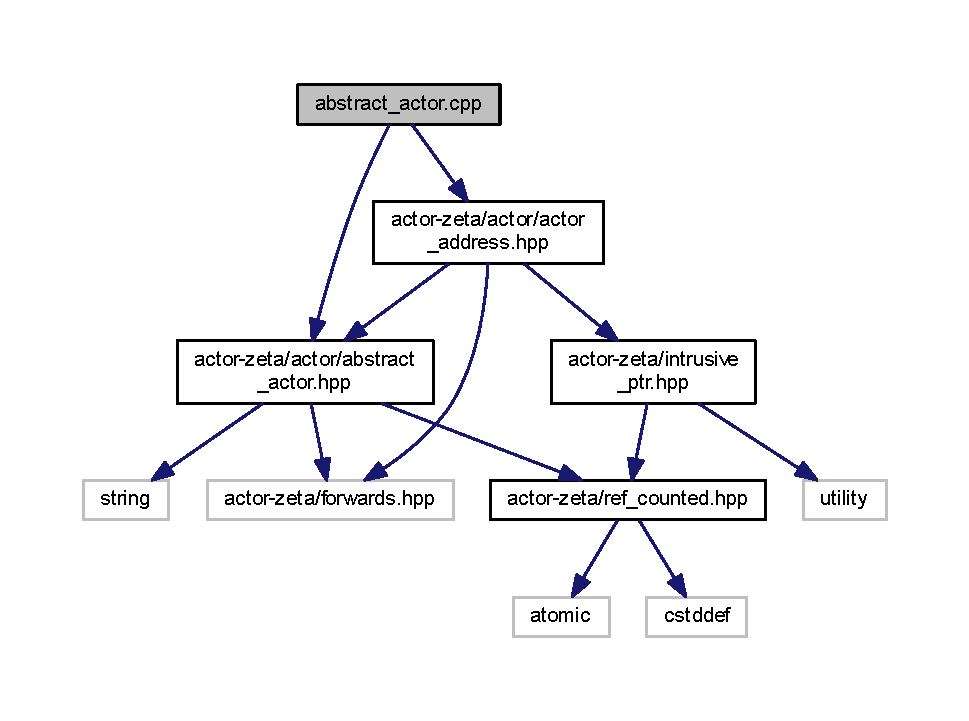
\includegraphics[width=350pt]{abstract__actor_8cpp__incl}
\end{center}
\end{figure}
\subsection*{Namespaces}
\begin{DoxyCompactItemize}
\item 
 \hyperlink{namespaceactor__zeta}{actor\+\_\+zeta}
\item 
 \hyperlink{namespaceactor__zeta_1_1actor}{actor\+\_\+zeta\+::actor}
\end{DoxyCompactItemize}

\hypertarget{abstract__actor_8hpp}{}\section{abstract\+\_\+actor.\+hpp File Reference}
\label{abstract__actor_8hpp}\index{abstract\+\_\+actor.\+hpp@{abstract\+\_\+actor.\+hpp}}
{\ttfamily \#include $<$string$>$}\newline
{\ttfamily \#include \char`\"{}actor-\/zeta/ref\+\_\+counted.\+hpp\char`\"{}}\newline
{\ttfamily \#include \char`\"{}actor-\/zeta/forwards.\+hpp\char`\"{}}\newline
Include dependency graph for abstract\+\_\+actor.\+hpp\+:\nopagebreak
\begin{figure}[H]
\begin{center}
\leavevmode
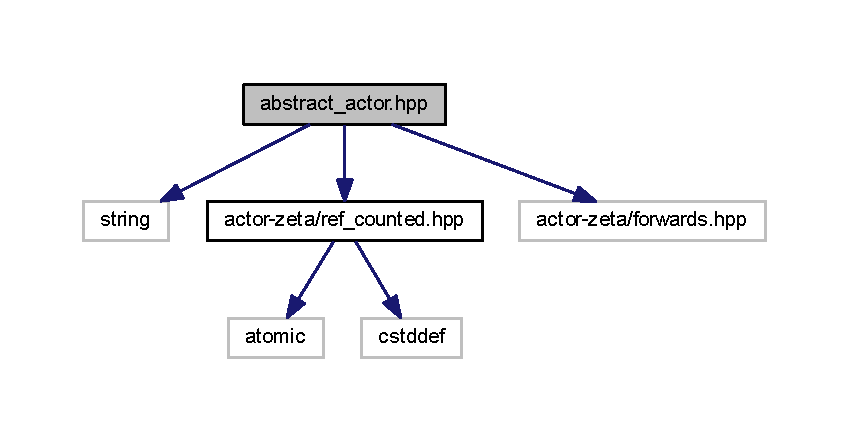
\includegraphics[width=350pt]{abstract__actor_8hpp__incl}
\end{center}
\end{figure}
This graph shows which files directly or indirectly include this file\+:\nopagebreak
\begin{figure}[H]
\begin{center}
\leavevmode
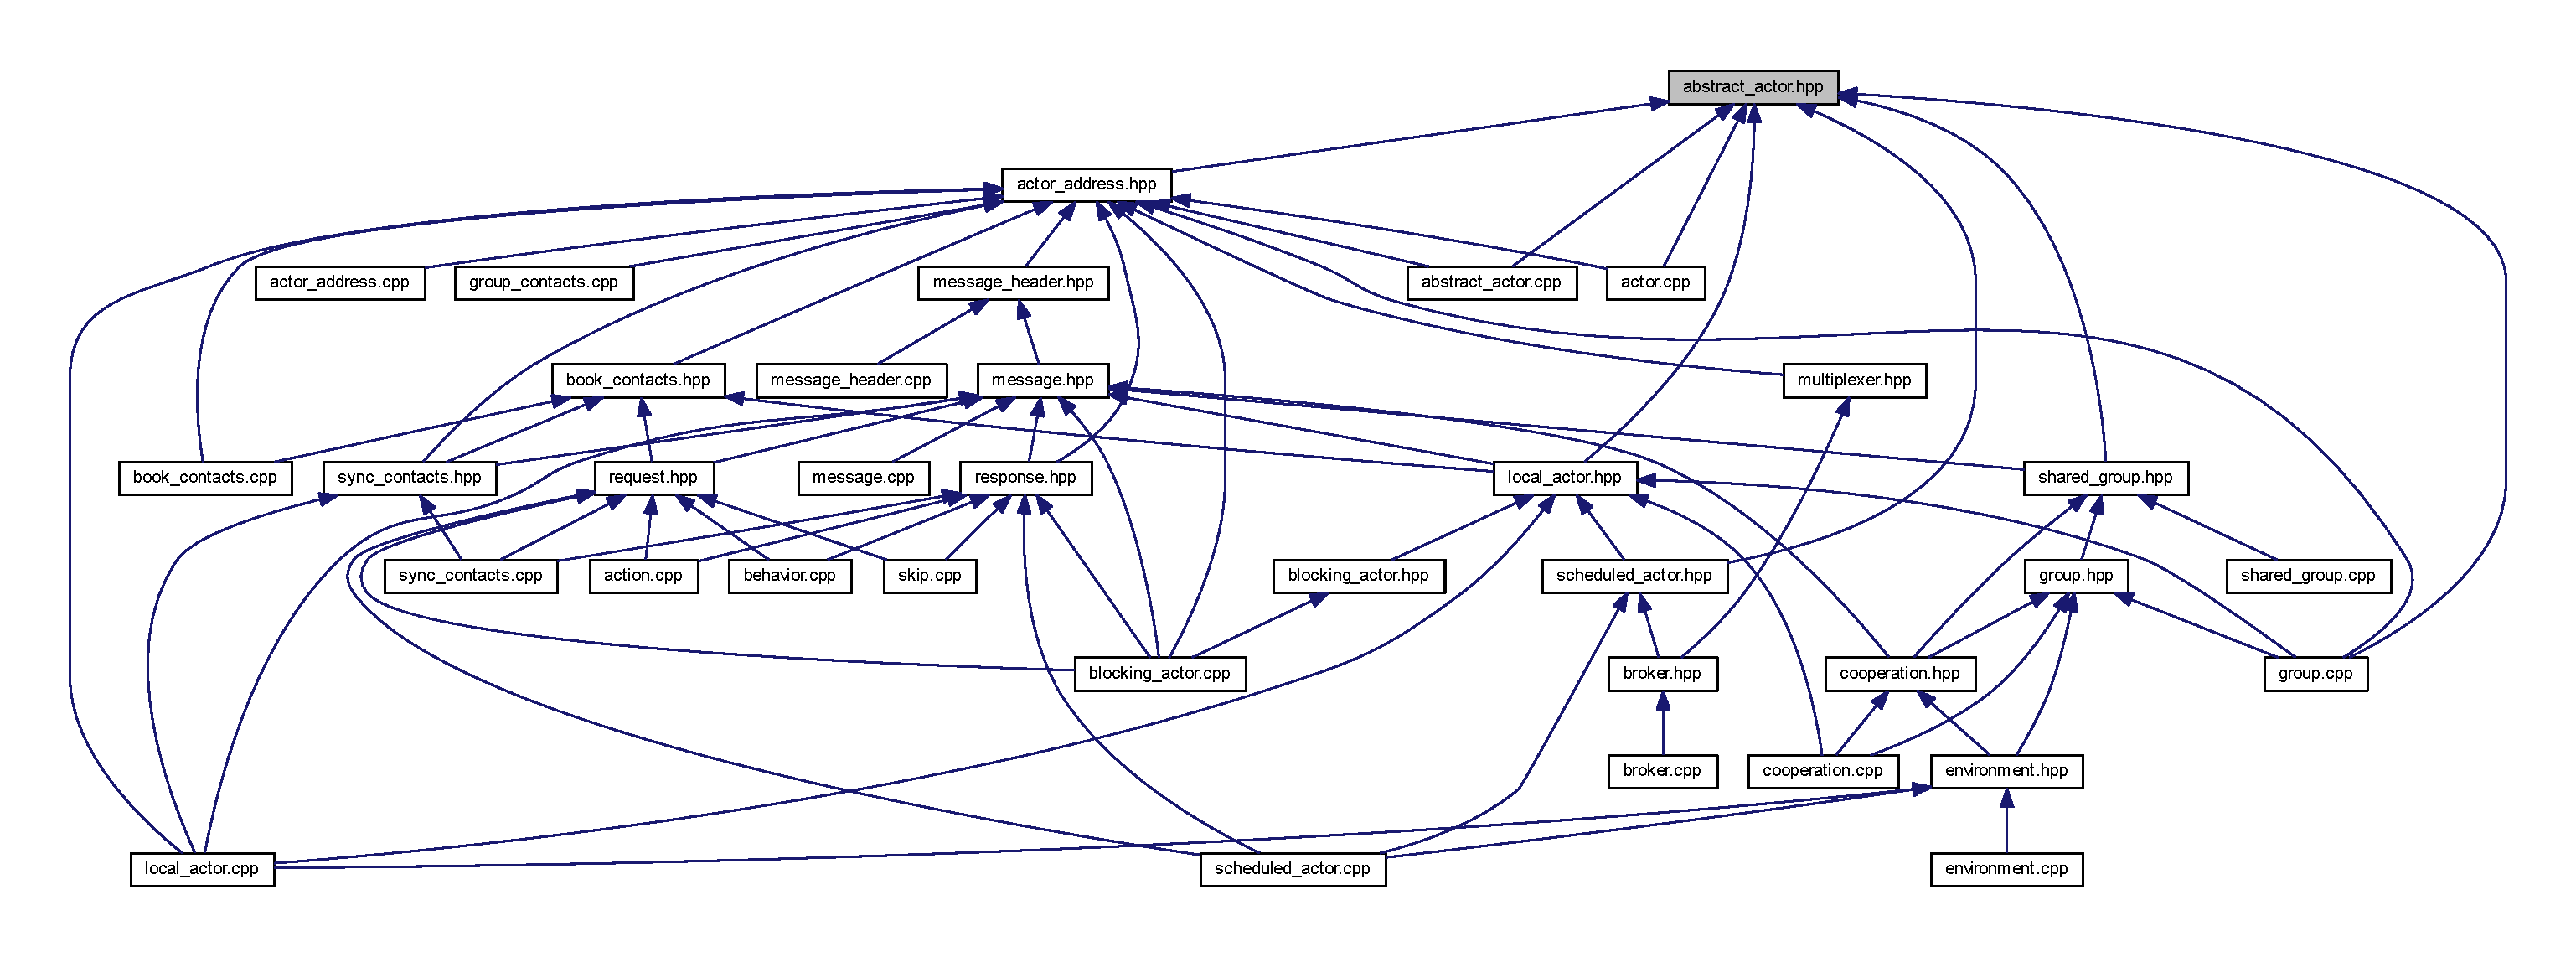
\includegraphics[width=350pt]{abstract__actor_8hpp__dep__incl}
\end{center}
\end{figure}
\subsection*{Classes}
\begin{DoxyCompactItemize}
\item 
class \hyperlink{classactor__zeta_1_1actor_1_1abstract__actor}{actor\+\_\+zeta\+::actor\+::abstract\+\_\+actor}
\begin{DoxyCompactList}\small\item\em abstract concept of an actor \end{DoxyCompactList}\end{DoxyCompactItemize}
\subsection*{Namespaces}
\begin{DoxyCompactItemize}
\item 
 \hyperlink{namespaceactor__zeta}{actor\+\_\+zeta}
\item 
 \hyperlink{namespaceactor__zeta_1_1actor}{actor\+\_\+zeta\+::actor}
\end{DoxyCompactItemize}

\hypertarget{abstract__coordinator_8hpp}{}\section{abstract\+\_\+coordinator.\+hpp File Reference}
\label{abstract__coordinator_8hpp}\index{abstract\+\_\+coordinator.\+hpp@{abstract\+\_\+coordinator.\+hpp}}
{\ttfamily \#include $<$thread$>$}\newline
{\ttfamily \#include \char`\"{}time\+\_\+unit.\+hpp\char`\"{}}\newline
{\ttfamily \#include \char`\"{}actor-\/zeta/forwards.\+hpp\char`\"{}}\newline
Include dependency graph for abstract\+\_\+coordinator.\+hpp\+:\nopagebreak
\begin{figure}[H]
\begin{center}
\leavevmode
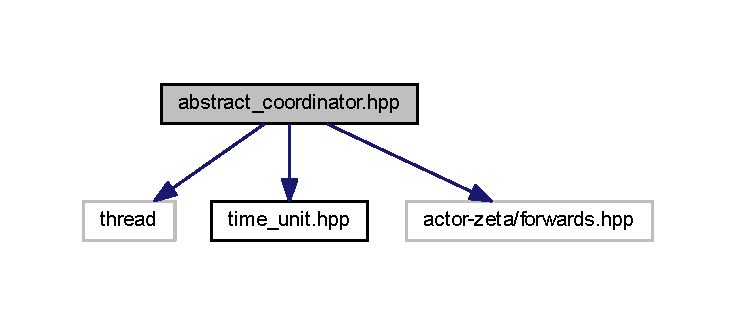
\includegraphics[width=350pt]{abstract__coordinator_8hpp__incl}
\end{center}
\end{figure}
This graph shows which files directly or indirectly include this file\+:\nopagebreak
\begin{figure}[H]
\begin{center}
\leavevmode
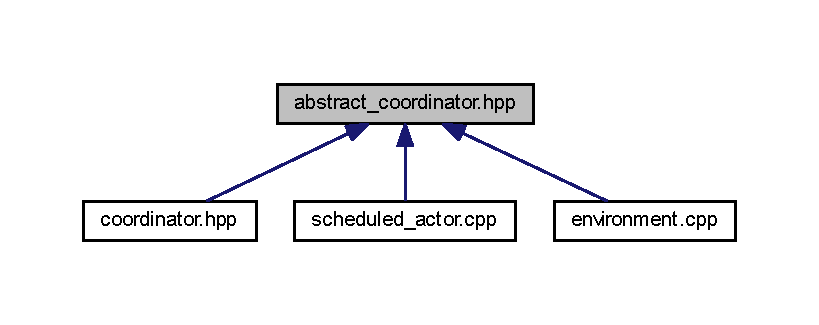
\includegraphics[width=350pt]{abstract__coordinator_8hpp__dep__incl}
\end{center}
\end{figure}
\subsection*{Classes}
\begin{DoxyCompactItemize}
\item 
class \hyperlink{classactor__zeta_1_1executor_1_1abstract__coordinator}{actor\+\_\+zeta\+::executor\+::abstract\+\_\+coordinator}
\begin{DoxyCompactList}\small\item\em abstract concept of an coordination approach \end{DoxyCompactList}\end{DoxyCompactItemize}
\subsection*{Namespaces}
\begin{DoxyCompactItemize}
\item 
 \hyperlink{namespaceactor__zeta}{actor\+\_\+zeta}
\item 
 \hyperlink{namespaceactor__zeta_1_1executor}{actor\+\_\+zeta\+::executor}
\end{DoxyCompactItemize}

\hypertarget{action_8cpp}{}\section{action.\+cpp File Reference}
\label{action_8cpp}\index{action.\+cpp@{action.\+cpp}}
{\ttfamily \#include \char`\"{}actor-\/zeta/behavior/action.\+hpp\char`\"{}}\newline
{\ttfamily \#include \char`\"{}actor-\/zeta/behavior/request.\+hpp\char`\"{}}\newline
{\ttfamily \#include \char`\"{}actor-\/zeta/behavior/response.\+hpp\char`\"{}}\newline
Include dependency graph for action.\+cpp\+:\nopagebreak
\begin{figure}[H]
\begin{center}
\leavevmode
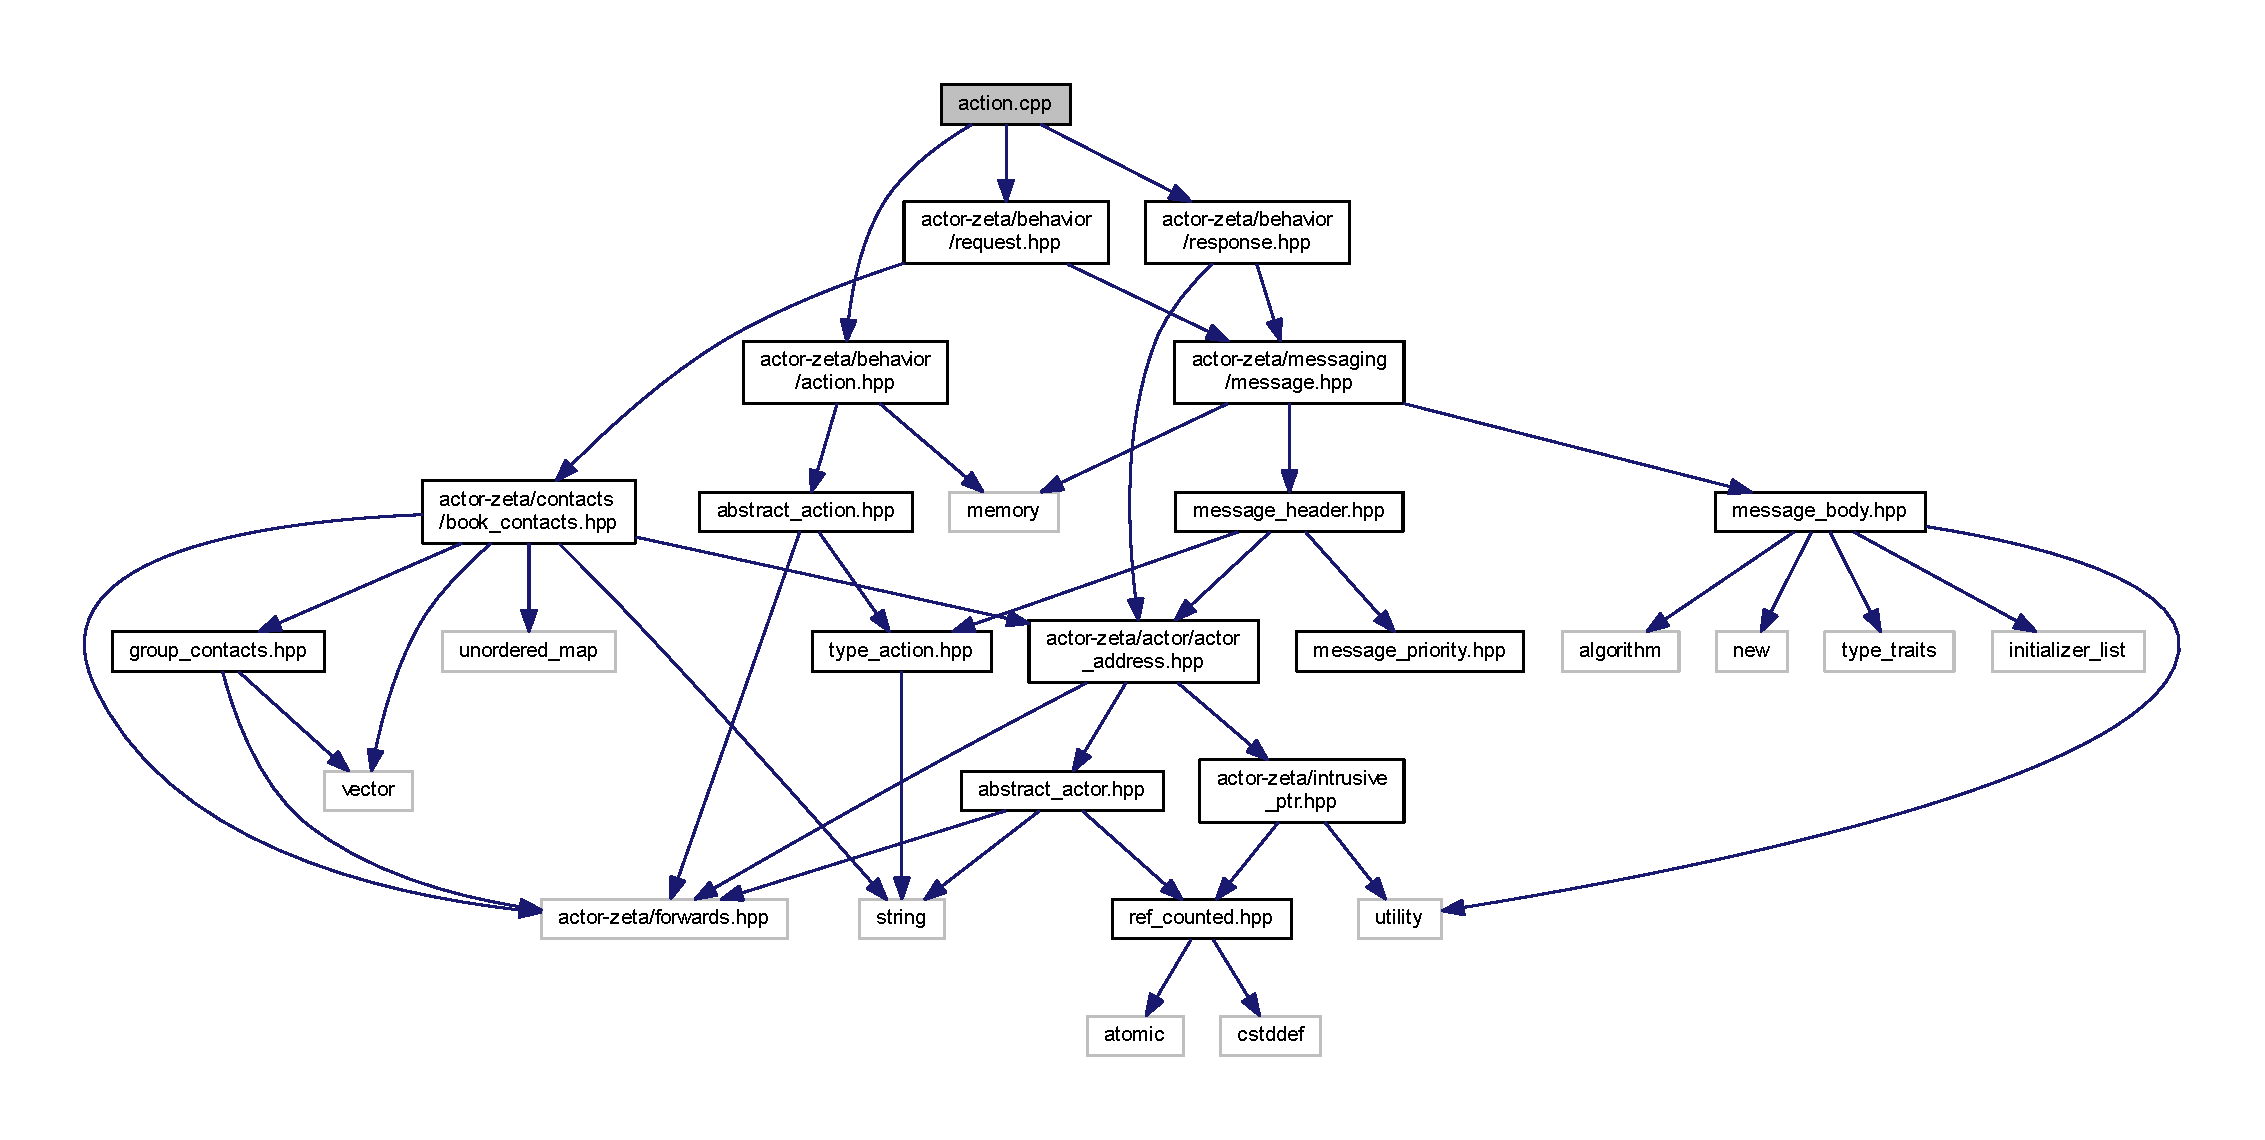
\includegraphics[width=350pt]{action_8cpp__incl}
\end{center}
\end{figure}
\subsection*{Namespaces}
\begin{DoxyCompactItemize}
\item 
 \hyperlink{namespaceactor__zeta}{actor\+\_\+zeta}
\item 
 \hyperlink{namespaceactor__zeta_1_1behavior}{actor\+\_\+zeta\+::behavior}
\end{DoxyCompactItemize}

\hypertarget{action_8hpp}{}\section{action.\+hpp File Reference}
\label{action_8hpp}\index{action.\+hpp@{action.\+hpp}}
{\ttfamily \#include $<$memory$>$}\newline
{\ttfamily \#include \char`\"{}abstract\+\_\+action.\+hpp\char`\"{}}\newline
Include dependency graph for action.\+hpp\+:\nopagebreak
\begin{figure}[H]
\begin{center}
\leavevmode
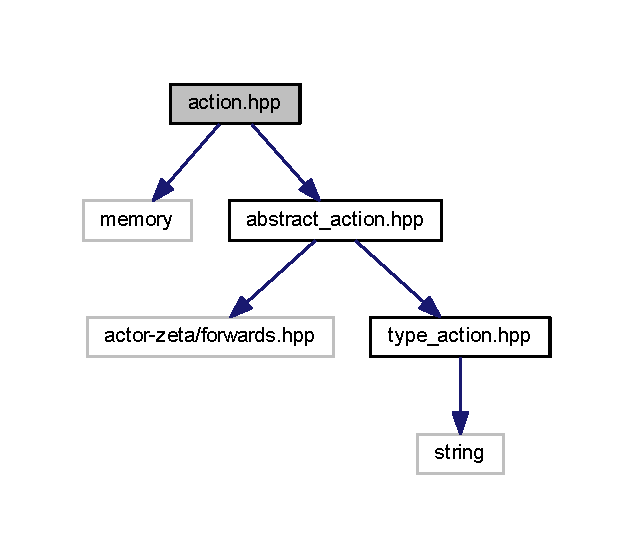
\includegraphics[width=304pt]{action_8hpp__incl}
\end{center}
\end{figure}
This graph shows which files directly or indirectly include this file\+:\nopagebreak
\begin{figure}[H]
\begin{center}
\leavevmode
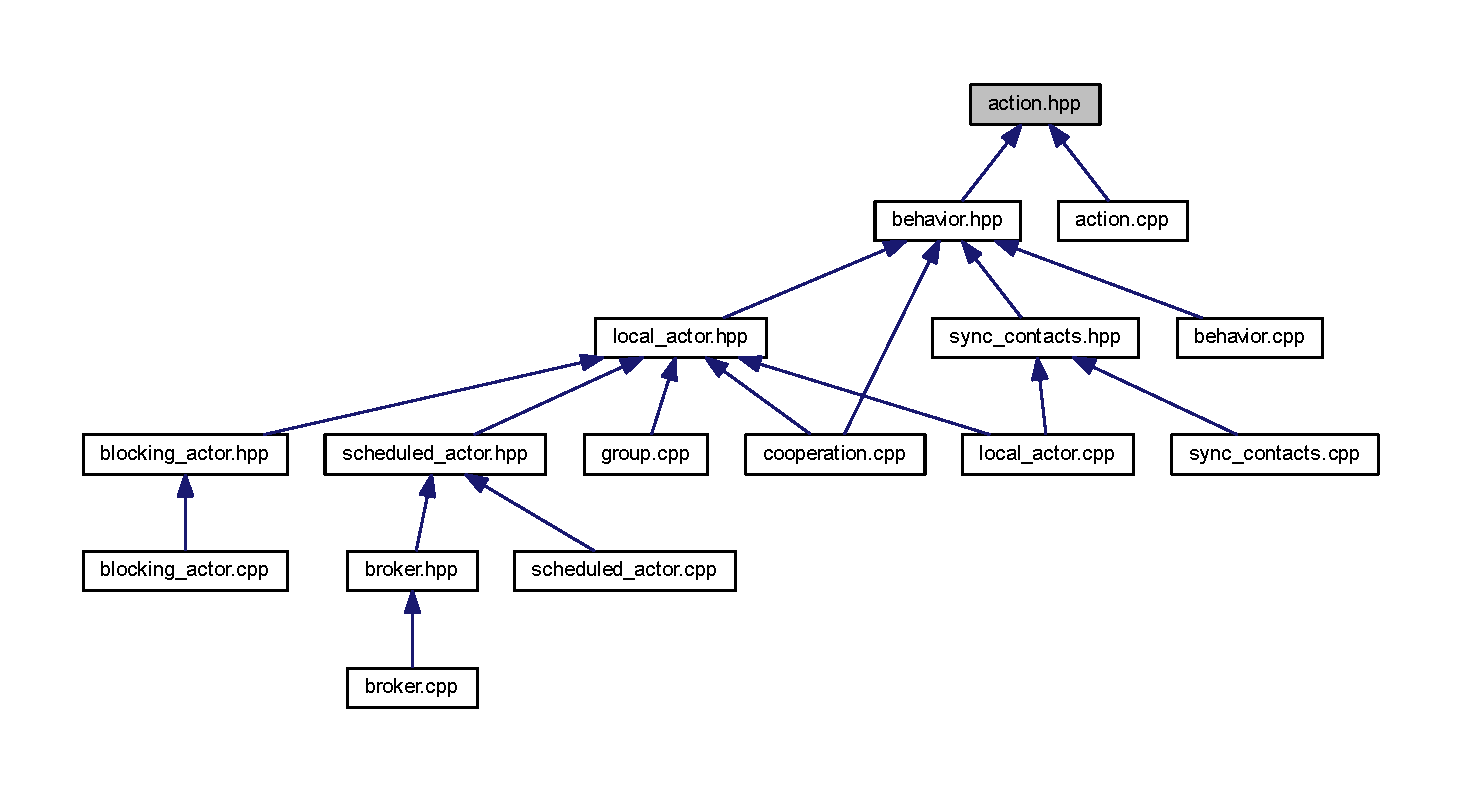
\includegraphics[width=350pt]{action_8hpp__dep__incl}
\end{center}
\end{figure}
\subsection*{Classes}
\begin{DoxyCompactItemize}
\item 
class \hyperlink{classactor__zeta_1_1behavior_1_1action}{actor\+\_\+zeta\+::behavior\+::action}
\begin{DoxyCompactList}\small\item\em Basic action implementation. \end{DoxyCompactList}\end{DoxyCompactItemize}
\subsection*{Namespaces}
\begin{DoxyCompactItemize}
\item 
 \hyperlink{namespaceactor__zeta}{actor\+\_\+zeta}
\item 
 \hyperlink{namespaceactor__zeta_1_1behavior}{actor\+\_\+zeta\+::behavior}
\end{DoxyCompactItemize}

\hypertarget{actor_8cpp}{}\section{actor.\+cpp File Reference}
\label{actor_8cpp}\index{actor.\+cpp@{actor.\+cpp}}
{\ttfamily \#include \char`\"{}actor-\/zeta/actor/actor.\+hpp\char`\"{}}\newline
{\ttfamily \#include \char`\"{}actor-\/zeta/actor/abstract\+\_\+actor.\+hpp\char`\"{}}\newline
{\ttfamily \#include \char`\"{}actor-\/zeta/actor/actor\+\_\+address.\+hpp\char`\"{}}\newline
Include dependency graph for actor.\+cpp\+:\nopagebreak
\begin{figure}[H]
\begin{center}
\leavevmode
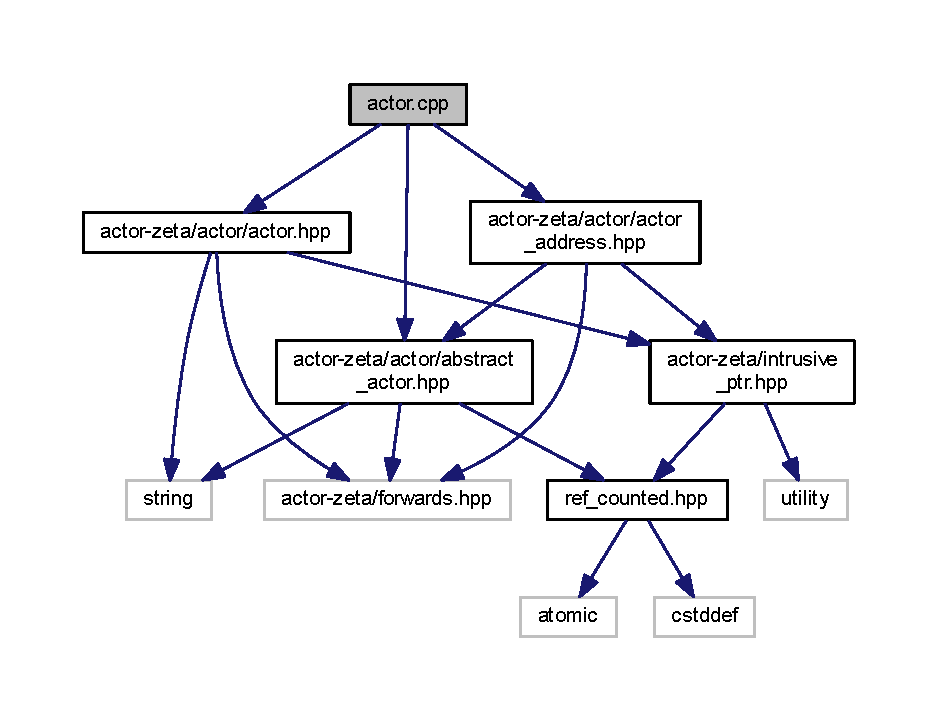
\includegraphics[width=350pt]{actor_8cpp__incl}
\end{center}
\end{figure}
\subsection*{Namespaces}
\begin{DoxyCompactItemize}
\item 
 \hyperlink{namespaceactor__zeta}{actor\+\_\+zeta}
\item 
 \hyperlink{namespaceactor__zeta_1_1actor}{actor\+\_\+zeta\+::actor}
\end{DoxyCompactItemize}

\hypertarget{actor_8hpp}{}\section{actor.\+hpp File Reference}
\label{actor_8hpp}\index{actor.\+hpp@{actor.\+hpp}}
{\ttfamily \#include $<$string$>$}\newline
{\ttfamily \#include \char`\"{}actor-\/zeta/intrusive\+\_\+ptr.\+hpp\char`\"{}}\newline
{\ttfamily \#include \char`\"{}actor-\/zeta/forwards.\+hpp\char`\"{}}\newline
Include dependency graph for actor.\+hpp\+:\nopagebreak
\begin{figure}[H]
\begin{center}
\leavevmode
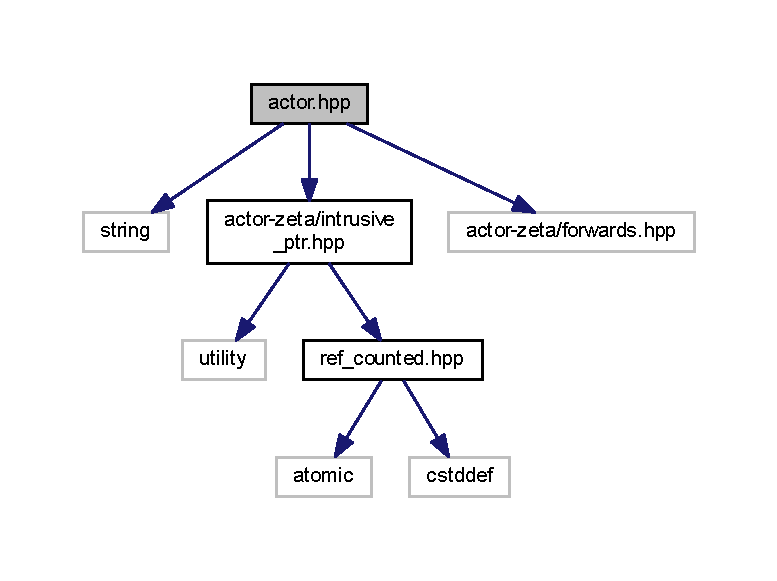
\includegraphics[width=350pt]{actor_8hpp__incl}
\end{center}
\end{figure}
This graph shows which files directly or indirectly include this file\+:\nopagebreak
\begin{figure}[H]
\begin{center}
\leavevmode
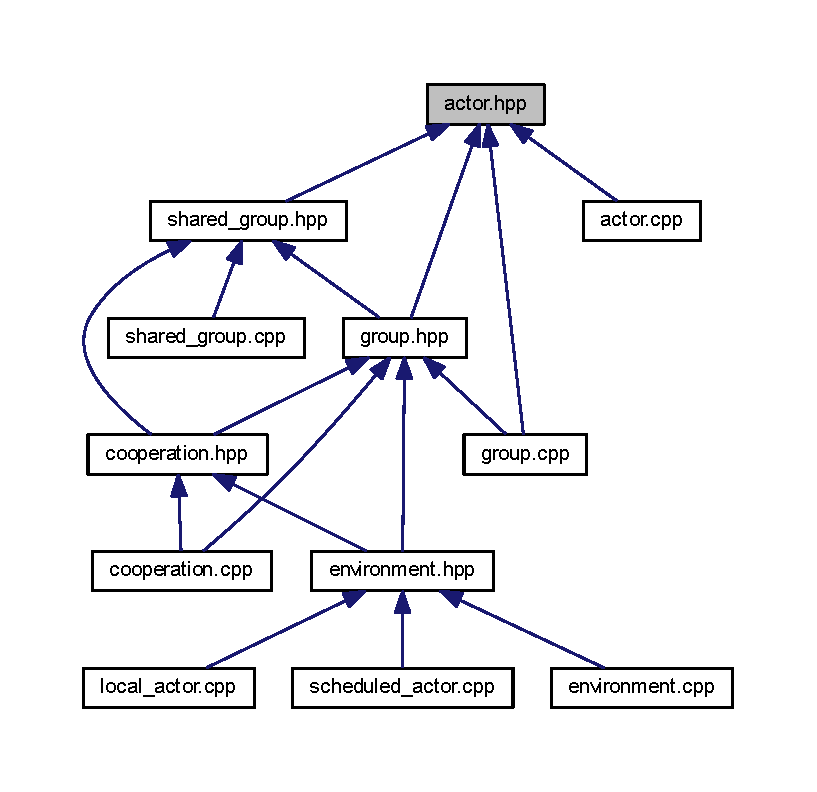
\includegraphics[width=350pt]{actor_8hpp__dep__incl}
\end{center}
\end{figure}
\subsection*{Classes}
\begin{DoxyCompactItemize}
\item 
class \hyperlink{classactor__zeta_1_1actor_1_1actor}{actor\+\_\+zeta\+::actor\+::actor}
\begin{DoxyCompactList}\small\item\em Basic actor implementation. \end{DoxyCompactList}\end{DoxyCompactItemize}
\subsection*{Namespaces}
\begin{DoxyCompactItemize}
\item 
 \hyperlink{namespaceactor__zeta}{actor\+\_\+zeta}
\item 
 \hyperlink{namespaceactor__zeta_1_1actor}{actor\+\_\+zeta\+::actor}
\end{DoxyCompactItemize}

\hypertarget{actor__address_8cpp}{}\section{actor\+\_\+address.\+cpp File Reference}
\label{actor__address_8cpp}\index{actor\+\_\+address.\+cpp@{actor\+\_\+address.\+cpp}}
{\ttfamily \#include \char`\"{}actor-\/zeta/actor/actor\+\_\+address.\+hpp\char`\"{}}\newline
Include dependency graph for actor\+\_\+address.\+cpp\+:\nopagebreak
\begin{figure}[H]
\begin{center}
\leavevmode
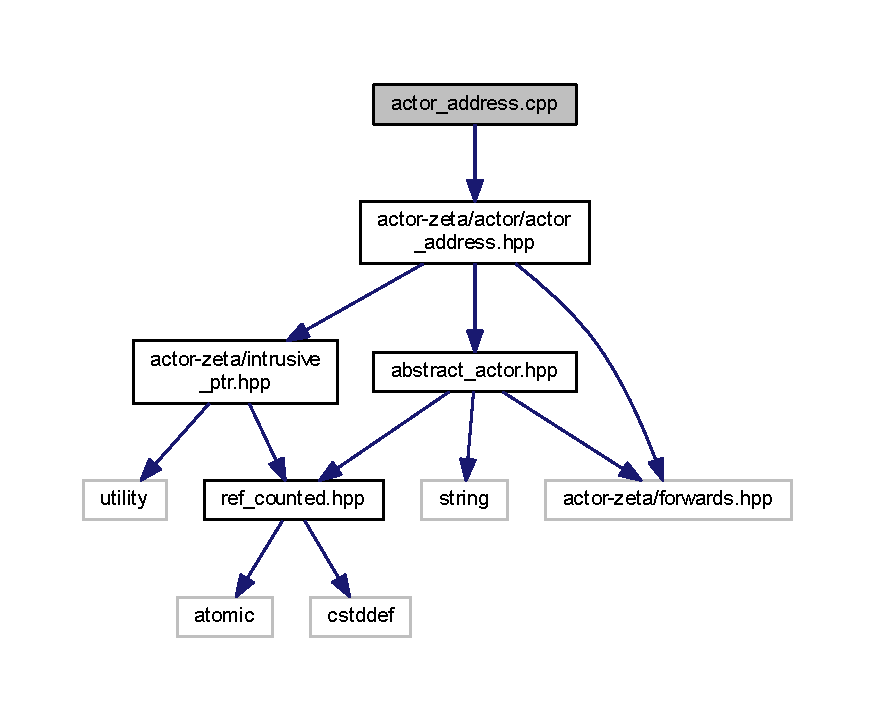
\includegraphics[width=350pt]{actor__address_8cpp__incl}
\end{center}
\end{figure}
\subsection*{Namespaces}
\begin{DoxyCompactItemize}
\item 
 \hyperlink{namespaceactor__zeta}{actor\+\_\+zeta}
\item 
 \hyperlink{namespaceactor__zeta_1_1actor}{actor\+\_\+zeta\+::actor}
\end{DoxyCompactItemize}

\hypertarget{actor__address_8hpp}{}\section{actor\+\_\+address.\+hpp File Reference}
\label{actor__address_8hpp}\index{actor\+\_\+address.\+hpp@{actor\+\_\+address.\+hpp}}
{\ttfamily \#include \char`\"{}actor-\/zeta/intrusive\+\_\+ptr.\+hpp\char`\"{}}\newline
{\ttfamily \#include \char`\"{}abstract\+\_\+actor.\+hpp\char`\"{}}\newline
{\ttfamily \#include \char`\"{}actor-\/zeta/forwards.\+hpp\char`\"{}}\newline
Include dependency graph for actor\+\_\+address.\+hpp\+:\nopagebreak
\begin{figure}[H]
\begin{center}
\leavevmode
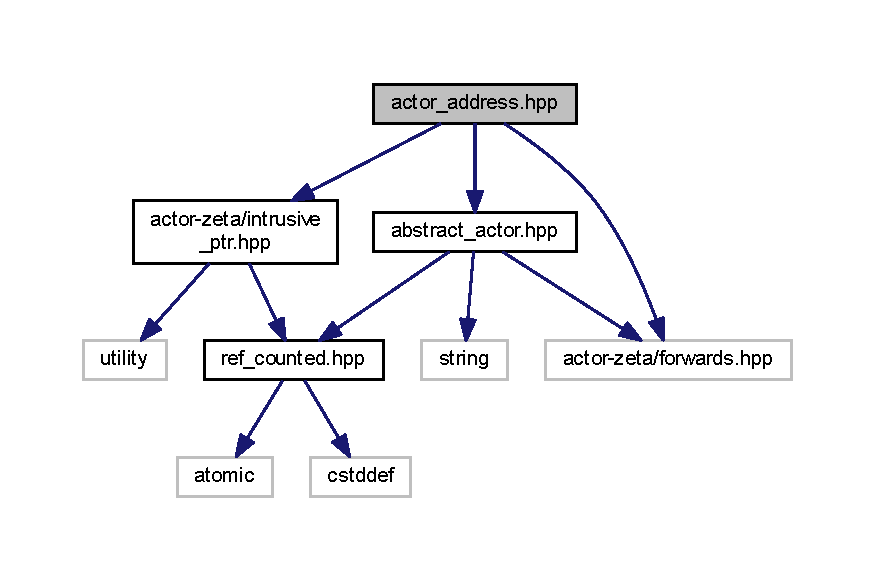
\includegraphics[width=350pt]{actor__address_8hpp__incl}
\end{center}
\end{figure}
This graph shows which files directly or indirectly include this file\+:\nopagebreak
\begin{figure}[H]
\begin{center}
\leavevmode
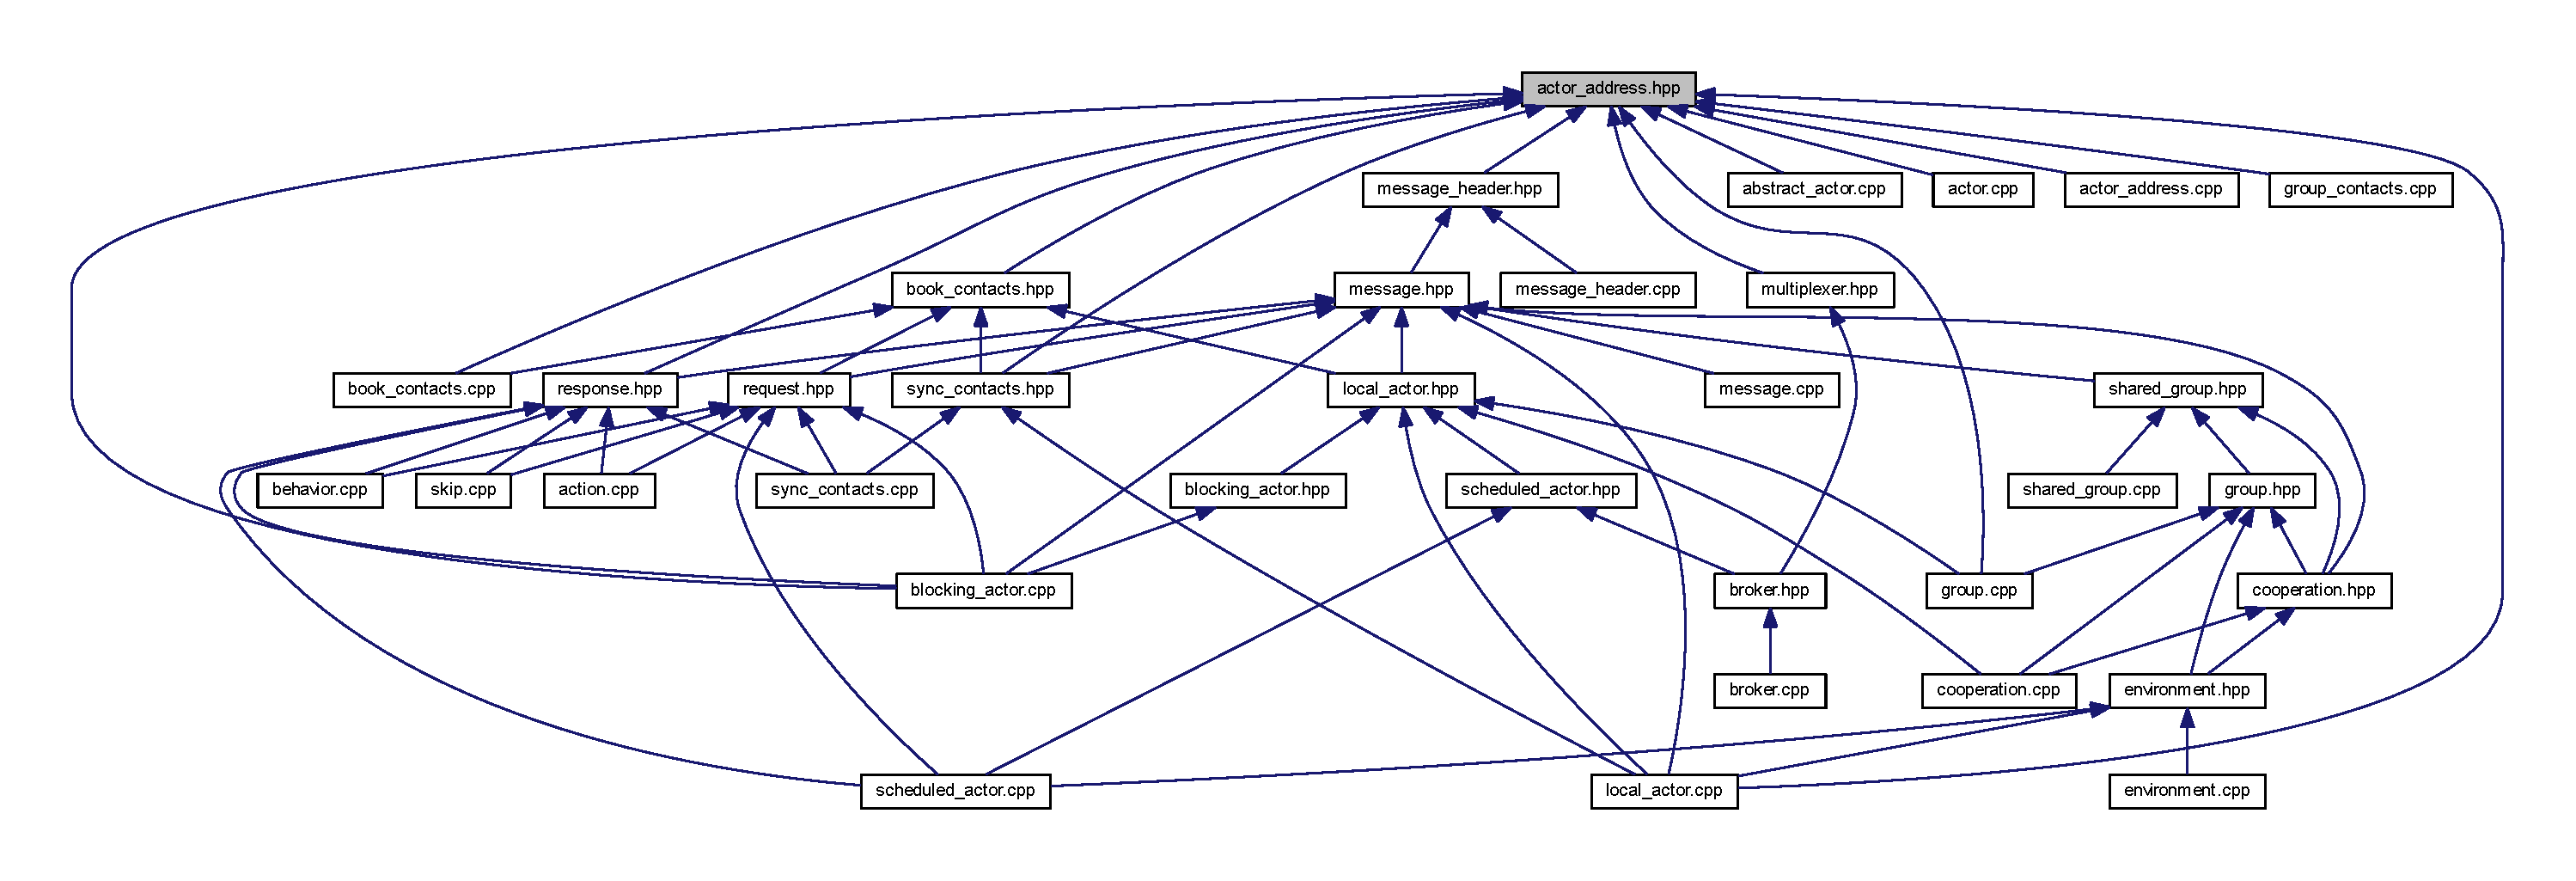
\includegraphics[width=350pt]{actor__address_8hpp__dep__incl}
\end{center}
\end{figure}
\subsection*{Classes}
\begin{DoxyCompactItemize}
\item 
class \hyperlink{classactor__zeta_1_1actor_1_1actor__address}{actor\+\_\+zeta\+::actor\+::actor\+\_\+address}
\begin{DoxyCompactList}\small\item\em This represents an actor\textquotesingle{}s address container. \end{DoxyCompactList}\end{DoxyCompactItemize}
\subsection*{Namespaces}
\begin{DoxyCompactItemize}
\item 
 \hyperlink{namespaceactor__zeta}{actor\+\_\+zeta}
\item 
 \hyperlink{namespaceactor__zeta_1_1actor}{actor\+\_\+zeta\+::actor}
\end{DoxyCompactItemize}

\hypertarget{behavior_8cpp}{}\section{behavior.\+cpp File Reference}
\label{behavior_8cpp}\index{behavior.\+cpp@{behavior.\+cpp}}
{\ttfamily \#include $<$initializer\+\_\+list$>$}\newline
{\ttfamily \#include \char`\"{}iostream\char`\"{}}\newline
{\ttfamily \#include \char`\"{}actor-\/zeta/behavior/behavior.\+hpp\char`\"{}}\newline
{\ttfamily \#include \char`\"{}actor-\/zeta/behavior/request.\+hpp\char`\"{}}\newline
{\ttfamily \#include \char`\"{}actor-\/zeta/behavior/response.\+hpp\char`\"{}}\newline
Include dependency graph for behavior.\+cpp\+:\nopagebreak
\begin{figure}[H]
\begin{center}
\leavevmode
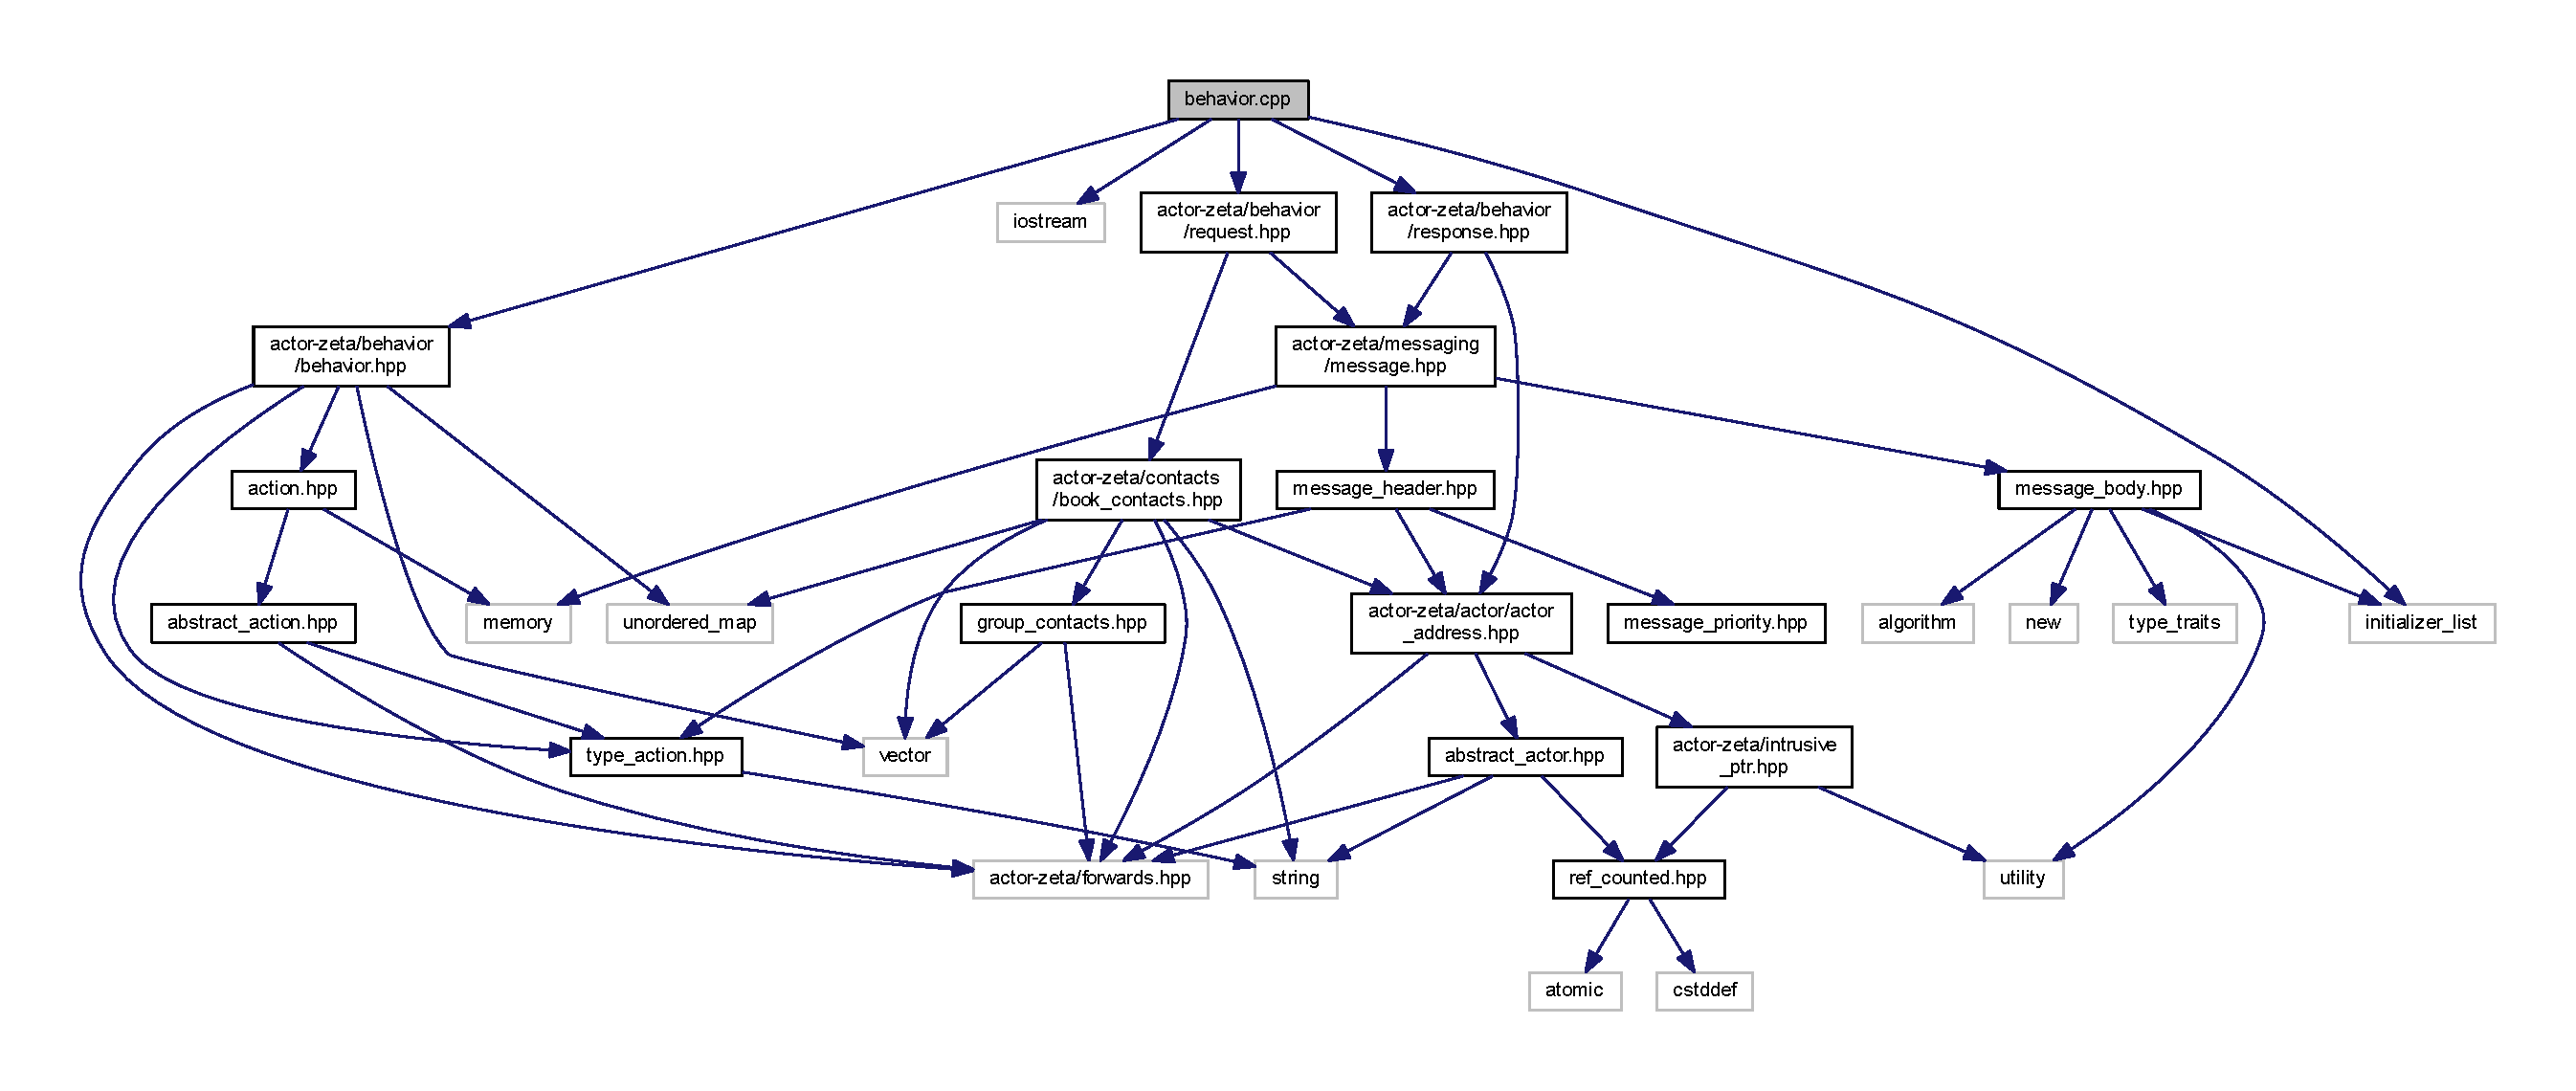
\includegraphics[width=350pt]{behavior_8cpp__incl}
\end{center}
\end{figure}
\subsection*{Namespaces}
\begin{DoxyCompactItemize}
\item 
 \hyperlink{namespaceactor__zeta}{actor\+\_\+zeta}
\item 
 \hyperlink{namespaceactor__zeta_1_1behavior}{actor\+\_\+zeta\+::behavior}
\end{DoxyCompactItemize}

\hypertarget{behavior_8hpp}{}\section{behavior.\+hpp File Reference}
\label{behavior_8hpp}\index{behavior.\+hpp@{behavior.\+hpp}}
{\ttfamily \#include $<$unordered\+\_\+map$>$}\newline
{\ttfamily \#include $<$vector$>$}\newline
{\ttfamily \#include \char`\"{}actor-\/zeta/forwards.\+hpp\char`\"{}}\newline
{\ttfamily \#include \char`\"{}action.\+hpp\char`\"{}}\newline
{\ttfamily \#include \char`\"{}type\+\_\+action.\+hpp\char`\"{}}\newline
Include dependency graph for behavior.\+hpp\+:\nopagebreak
\begin{figure}[H]
\begin{center}
\leavevmode
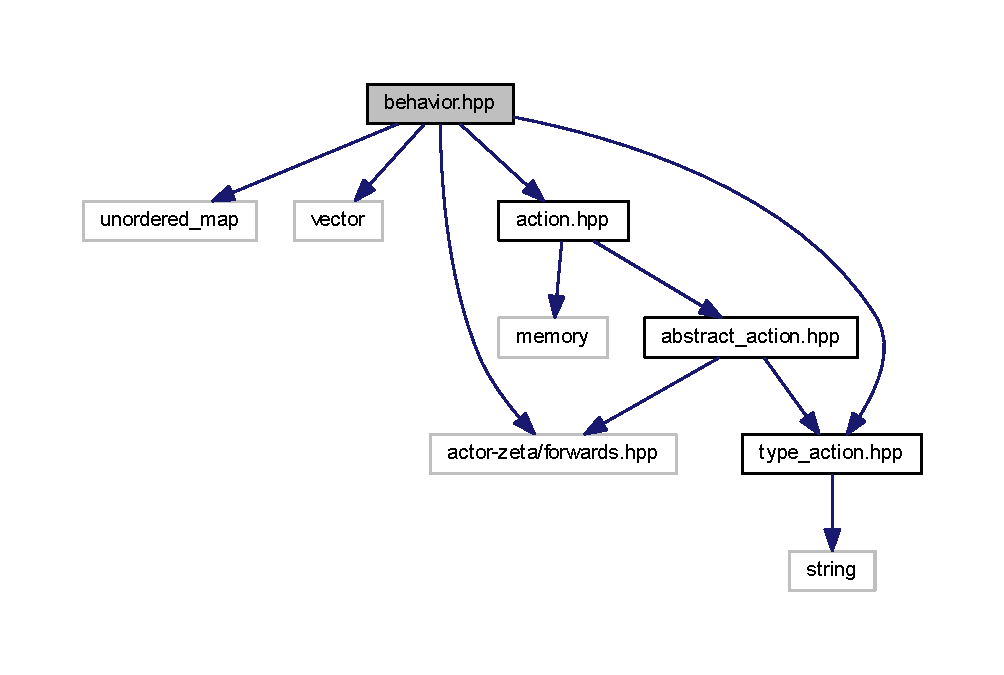
\includegraphics[width=350pt]{behavior_8hpp__incl}
\end{center}
\end{figure}
This graph shows which files directly or indirectly include this file\+:\nopagebreak
\begin{figure}[H]
\begin{center}
\leavevmode
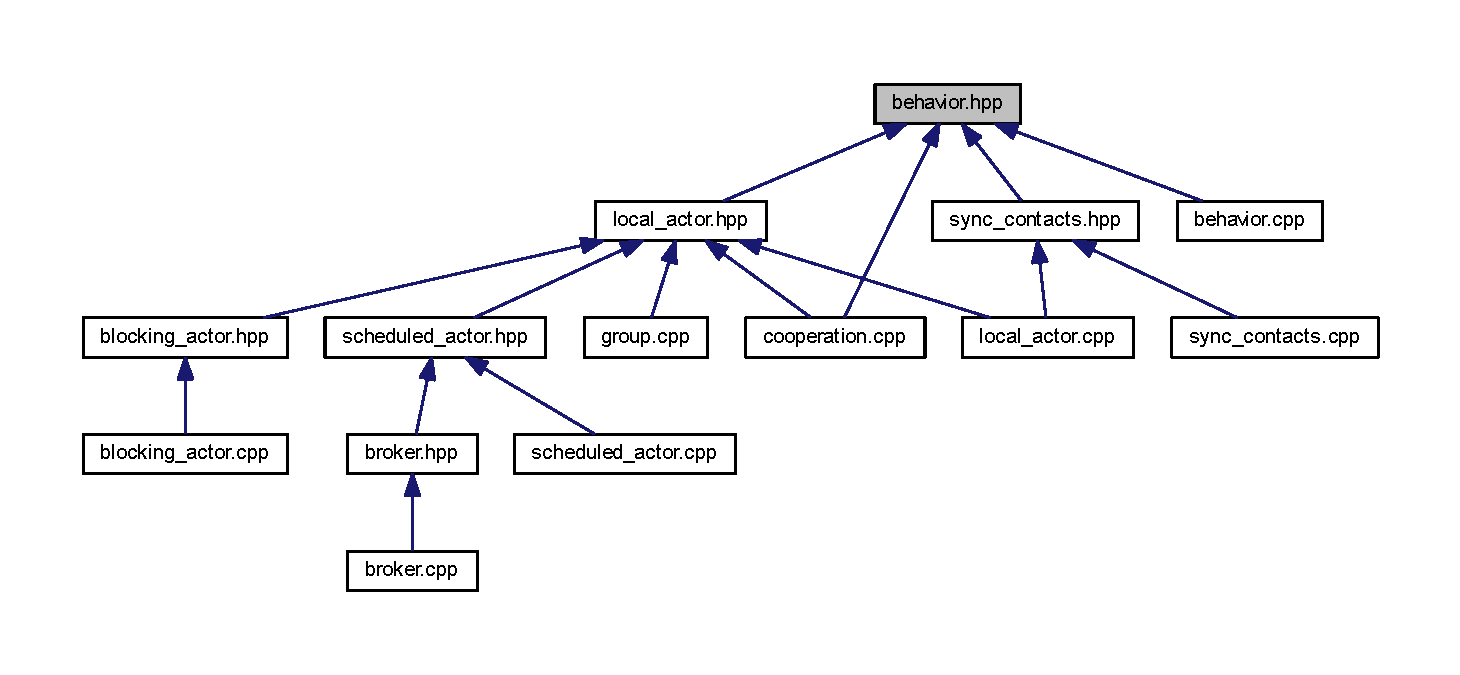
\includegraphics[width=350pt]{behavior_8hpp__dep__incl}
\end{center}
\end{figure}
\subsection*{Classes}
\begin{DoxyCompactItemize}
\item 
class \hyperlink{classactor__zeta_1_1behavior_1_1behavior}{actor\+\_\+zeta\+::behavior\+::behavior}
\begin{DoxyCompactList}\small\item\em Class for lyfecycle determination. \end{DoxyCompactList}\end{DoxyCompactItemize}
\subsection*{Namespaces}
\begin{DoxyCompactItemize}
\item 
 \hyperlink{namespaceactor__zeta}{actor\+\_\+zeta}
\item 
 \hyperlink{namespaceactor__zeta_1_1behavior}{actor\+\_\+zeta\+::behavior}
\end{DoxyCompactItemize}

\hypertarget{blocking__actor_8cpp}{}\section{blocking\+\_\+actor.\+cpp File Reference}
\label{blocking__actor_8cpp}\index{blocking\+\_\+actor.\+cpp@{blocking\+\_\+actor.\+cpp}}
{\ttfamily \#include \char`\"{}actor-\/zeta/actor/blocking\+\_\+actor.\+hpp\char`\"{}}\newline
{\ttfamily \#include \char`\"{}actor-\/zeta/executor/execution\+\_\+device.\+hpp\char`\"{}}\newline
{\ttfamily \#include \char`\"{}actor-\/zeta/actor/actor\+\_\+address.\+hpp\char`\"{}}\newline
{\ttfamily \#include \char`\"{}actor-\/zeta/messaging/message.\+hpp\char`\"{}}\newline
{\ttfamily \#include \char`\"{}actor-\/zeta/behavior/request.\+hpp\char`\"{}}\newline
{\ttfamily \#include \char`\"{}actor-\/zeta/behavior/response.\+hpp\char`\"{}}\newline
Include dependency graph for blocking\+\_\+actor.\+cpp\+:\nopagebreak
\begin{figure}[H]
\begin{center}
\leavevmode
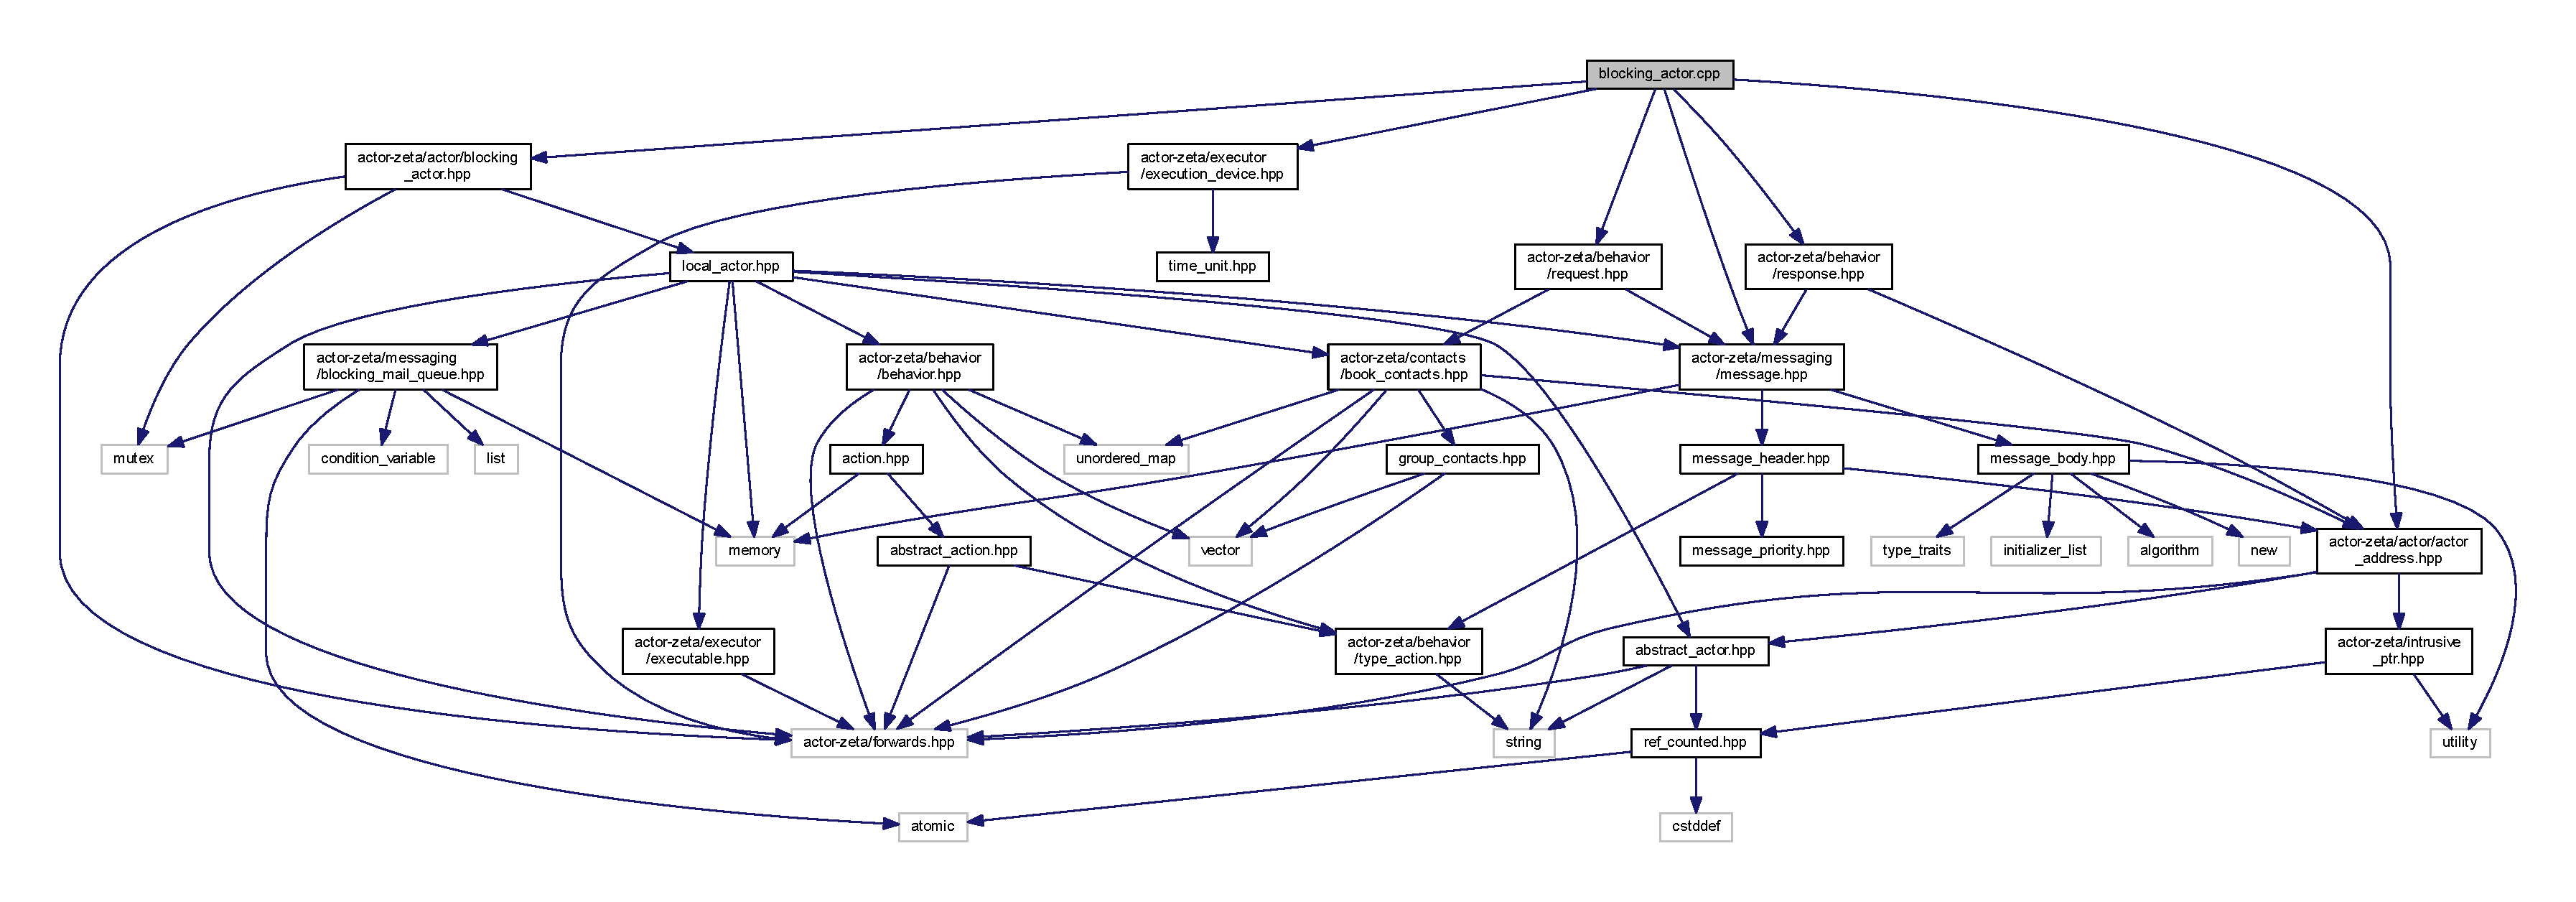
\includegraphics[width=350pt]{blocking__actor_8cpp__incl}
\end{center}
\end{figure}
\subsection*{Namespaces}
\begin{DoxyCompactItemize}
\item 
 \hyperlink{namespaceactor__zeta}{actor\+\_\+zeta}
\item 
 \hyperlink{namespaceactor__zeta_1_1actor}{actor\+\_\+zeta\+::actor}
\end{DoxyCompactItemize}

\hypertarget{blocking__actor_8hpp}{}\section{blocking\+\_\+actor.\+hpp File Reference}
\label{blocking__actor_8hpp}\index{blocking\+\_\+actor.\+hpp@{blocking\+\_\+actor.\+hpp}}
{\ttfamily \#include $<$mutex$>$}\newline
{\ttfamily \#include \char`\"{}actor-\/zeta/forwards.\+hpp\char`\"{}}\newline
{\ttfamily \#include \char`\"{}local\+\_\+actor.\+hpp\char`\"{}}\newline
Include dependency graph for blocking\+\_\+actor.\+hpp\+:\nopagebreak
\begin{figure}[H]
\begin{center}
\leavevmode
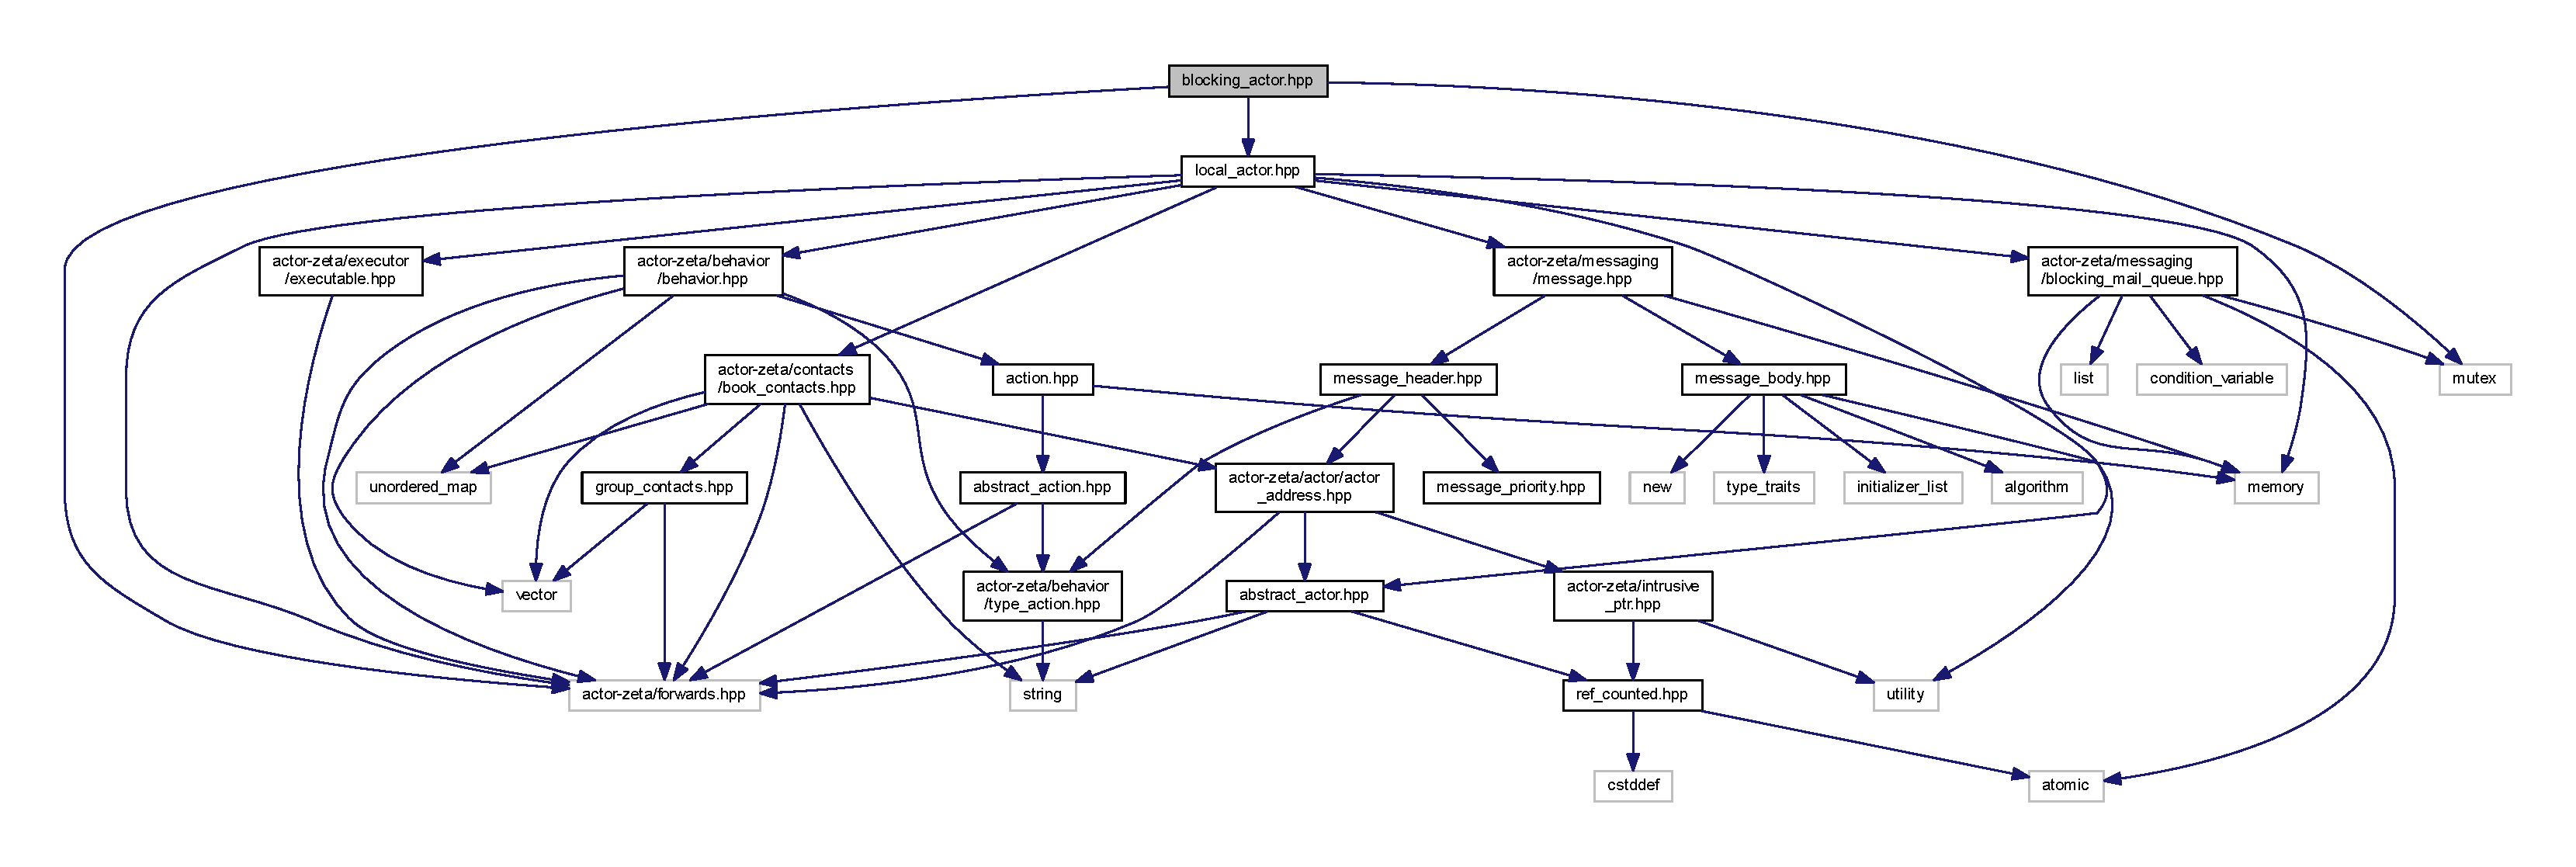
\includegraphics[width=350pt]{blocking__actor_8hpp__incl}
\end{center}
\end{figure}
This graph shows which files directly or indirectly include this file\+:\nopagebreak
\begin{figure}[H]
\begin{center}
\leavevmode
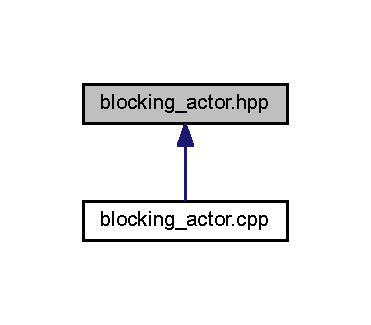
\includegraphics[width=178pt]{blocking__actor_8hpp__dep__incl}
\end{center}
\end{figure}
\subsection*{Classes}
\begin{DoxyCompactItemize}
\item 
class \hyperlink{classactor__zeta_1_1actor_1_1blocking__actor}{actor\+\_\+zeta\+::actor\+::blocking\+\_\+actor}
\begin{DoxyCompactList}\small\item\em Represents actor type with blocking mode. \end{DoxyCompactList}\end{DoxyCompactItemize}
\subsection*{Namespaces}
\begin{DoxyCompactItemize}
\item 
 \hyperlink{namespaceactor__zeta}{actor\+\_\+zeta}
\item 
 \hyperlink{namespaceactor__zeta_1_1actor}{actor\+\_\+zeta\+::actor}
\end{DoxyCompactItemize}

\hypertarget{blocking__mail__queue_8hpp}{}\section{blocking\+\_\+mail\+\_\+queue.\+hpp File Reference}
\label{blocking__mail__queue_8hpp}\index{blocking\+\_\+mail\+\_\+queue.\+hpp@{blocking\+\_\+mail\+\_\+queue.\+hpp}}
{\ttfamily \#include $<$mutex$>$}\newline
{\ttfamily \#include $<$condition\+\_\+variable$>$}\newline
{\ttfamily \#include $<$list$>$}\newline
{\ttfamily \#include $<$memory$>$}\newline
{\ttfamily \#include $<$atomic$>$}\newline
Include dependency graph for blocking\+\_\+mail\+\_\+queue.\+hpp\+:\nopagebreak
\begin{figure}[H]
\begin{center}
\leavevmode
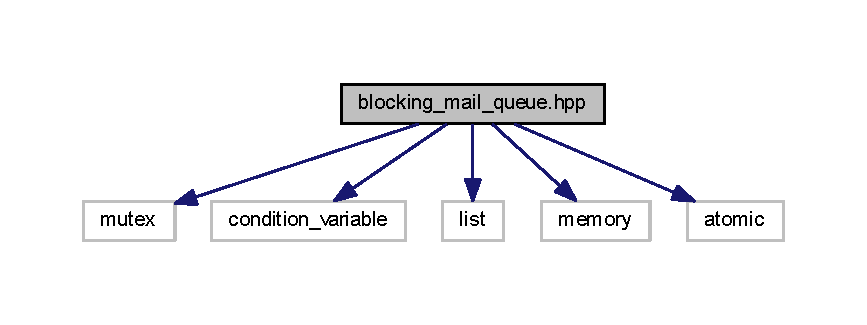
\includegraphics[width=350pt]{blocking__mail__queue_8hpp__incl}
\end{center}
\end{figure}
This graph shows which files directly or indirectly include this file\+:\nopagebreak
\begin{figure}[H]
\begin{center}
\leavevmode
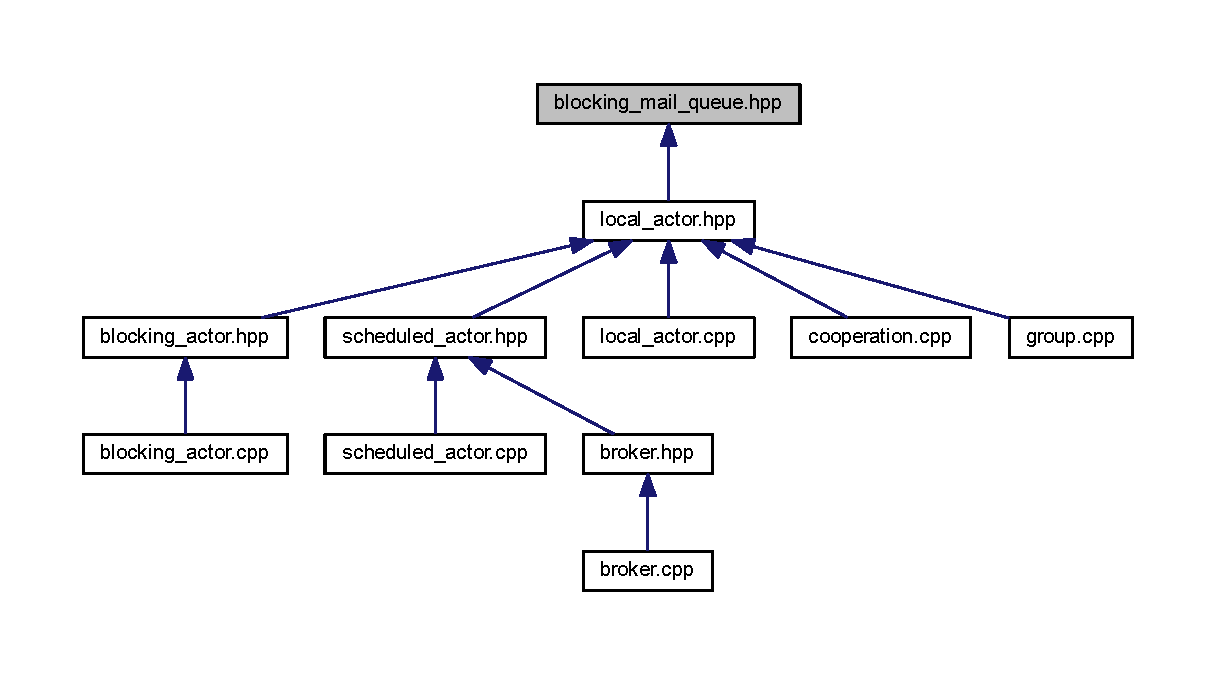
\includegraphics[width=350pt]{blocking__mail__queue_8hpp__dep__incl}
\end{center}
\end{figure}
\subsection*{Classes}
\begin{DoxyCompactItemize}
\item 
class \hyperlink{classactor__zeta_1_1messaging_1_1blocking__mail__queue}{actor\+\_\+zeta\+::messaging\+::blocking\+\_\+mail\+\_\+queue$<$ T $>$}
\begin{DoxyCompactList}\small\item\em A mailbox class for message queue. \end{DoxyCompactList}\end{DoxyCompactItemize}
\subsection*{Namespaces}
\begin{DoxyCompactItemize}
\item 
 \hyperlink{namespaceactor__zeta}{actor\+\_\+zeta}
\item 
 \hyperlink{namespaceactor__zeta_1_1messaging}{actor\+\_\+zeta\+::messaging}
\end{DoxyCompactItemize}
\subsection*{Enumerations}
\begin{DoxyCompactItemize}
\item 
enum \hyperlink{namespaceactor__zeta_1_1messaging_ac2c5f2f473c5a97d779ec63a78d498a1}{actor\+\_\+zeta\+::messaging\+::enqueue\+\_\+result} \{ \hyperlink{namespaceactor__zeta_1_1messaging_ac2c5f2f473c5a97d779ec63a78d498a1a260ca9dd8a4577fc00b7bd5810298076}{actor\+\_\+zeta\+::messaging\+::enqueue\+\_\+result\+::success}, 
\hyperlink{namespaceactor__zeta_1_1messaging_ac2c5f2f473c5a97d779ec63a78d498a1a8505d92f1a08d64e80ebffbde6749069}{actor\+\_\+zeta\+::messaging\+::enqueue\+\_\+result\+::unblocked\+\_\+reader}, 
\hyperlink{namespaceactor__zeta_1_1messaging_ac2c5f2f473c5a97d779ec63a78d498a1a1f494a6c8d9d6b854fcae46e258d9b85}{actor\+\_\+zeta\+::messaging\+::enqueue\+\_\+result\+::queue\+\_\+closed}
 \}\begin{DoxyCompactList}\small\item\em A strongly typed enum class representing enqueue result. \end{DoxyCompactList}
\end{DoxyCompactItemize}

\hypertarget{book__contacts_8cpp}{}\section{book\+\_\+contacts.\+cpp File Reference}
\label{book__contacts_8cpp}\index{book\+\_\+contacts.\+cpp@{book\+\_\+contacts.\+cpp}}
{\ttfamily \#include $<$iostream$>$}\newline
{\ttfamily \#include \char`\"{}actor-\/zeta/contacts/book\+\_\+contacts.\+hpp\char`\"{}}\newline
{\ttfamily \#include \char`\"{}actor-\/zeta/contacts/group\+\_\+contacts.\+hpp\char`\"{}}\newline
{\ttfamily \#include \char`\"{}actor-\/zeta/actor/actor\+\_\+address.\+hpp\char`\"{}}\newline
Include dependency graph for book\+\_\+contacts.\+cpp\+:\nopagebreak
\begin{figure}[H]
\begin{center}
\leavevmode
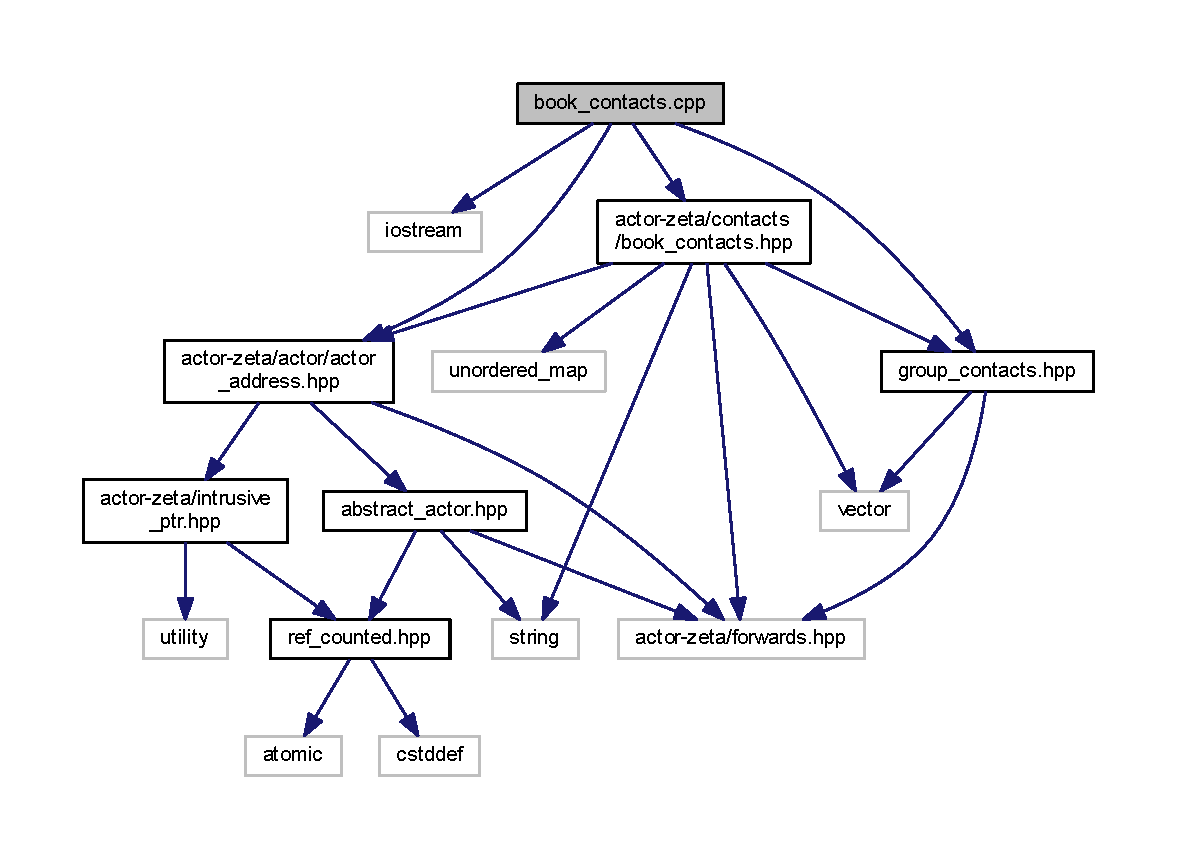
\includegraphics[width=350pt]{book__contacts_8cpp__incl}
\end{center}
\end{figure}
\subsection*{Namespaces}
\begin{DoxyCompactItemize}
\item 
 \hyperlink{namespaceactor__zeta}{actor\+\_\+zeta}
\item 
 \hyperlink{namespaceactor__zeta_1_1contacts}{actor\+\_\+zeta\+::contacts}
\end{DoxyCompactItemize}

\hypertarget{book__contacts_8hpp}{}\section{book\+\_\+contacts.\+hpp File Reference}
\label{book__contacts_8hpp}\index{book\+\_\+contacts.\+hpp@{book\+\_\+contacts.\+hpp}}
{\ttfamily \#include $<$string$>$}\newline
{\ttfamily \#include $<$vector$>$}\newline
{\ttfamily \#include $<$unordered\+\_\+map$>$}\newline
{\ttfamily \#include \char`\"{}actor-\/zeta/forwards.\+hpp\char`\"{}}\newline
{\ttfamily \#include \char`\"{}actor-\/zeta/actor/actor\+\_\+address.\+hpp\char`\"{}}\newline
{\ttfamily \#include \char`\"{}group\+\_\+contacts.\+hpp\char`\"{}}\newline
Include dependency graph for book\+\_\+contacts.\+hpp\+:\nopagebreak
\begin{figure}[H]
\begin{center}
\leavevmode
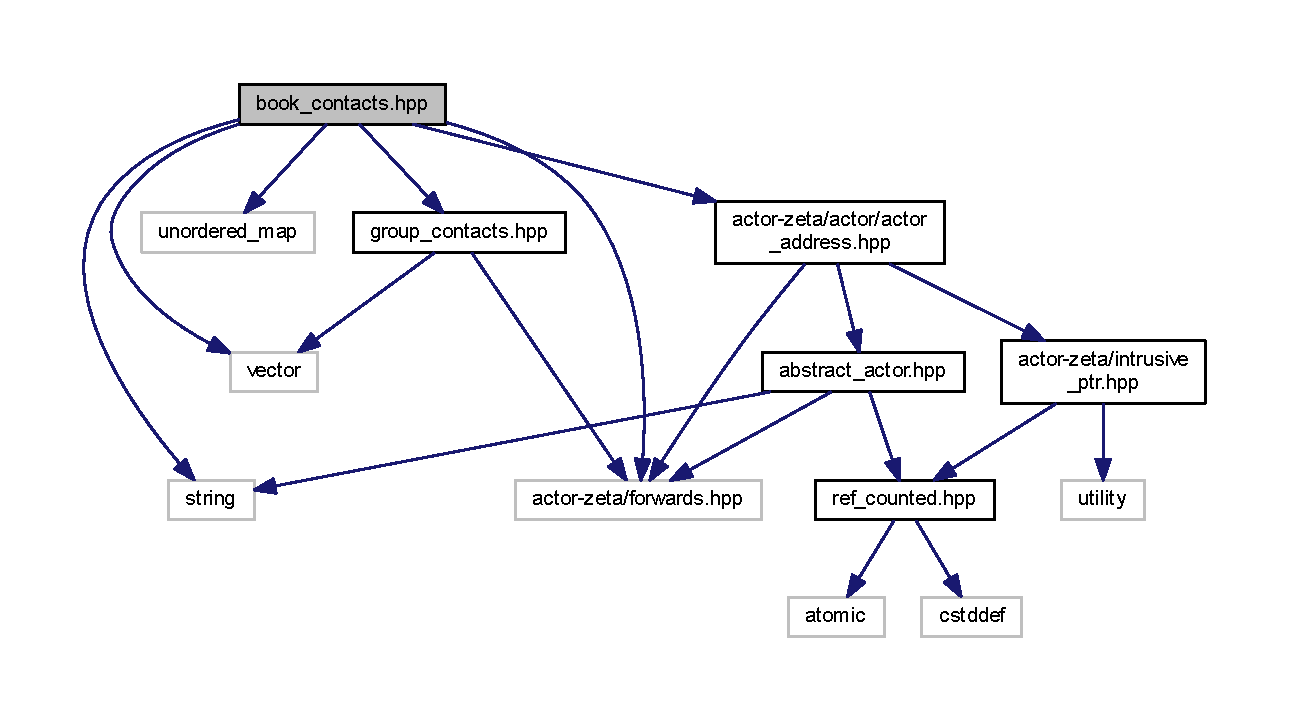
\includegraphics[width=350pt]{book__contacts_8hpp__incl}
\end{center}
\end{figure}
This graph shows which files directly or indirectly include this file\+:\nopagebreak
\begin{figure}[H]
\begin{center}
\leavevmode
\includegraphics[width=350pt]{book__contacts_8hpp__dep__incl}
\end{center}
\end{figure}
\subsection*{Classes}
\begin{DoxyCompactItemize}
\item 
class \hyperlink{classactor__zeta_1_1contacts_1_1book__contacts}{actor\+\_\+zeta\+::contacts\+::book\+\_\+contacts}
\begin{DoxyCompactList}\small\item\em Navigation map for actor \& groups. \end{DoxyCompactList}\end{DoxyCompactItemize}
\subsection*{Namespaces}
\begin{DoxyCompactItemize}
\item 
 \hyperlink{namespaceactor__zeta}{actor\+\_\+zeta}
\item 
 \hyperlink{namespaceactor__zeta_1_1contacts}{actor\+\_\+zeta\+::contacts}
\end{DoxyCompactItemize}

\hypertarget{broker_8cpp}{}\section{broker.\+cpp File Reference}
\label{broker_8cpp}\index{broker.\+cpp@{broker.\+cpp}}
{\ttfamily \#include \char`\"{}actor-\/zeta/actor/broker.\+hpp\char`\"{}}\newline
Include dependency graph for broker.\+cpp\+:\nopagebreak
\begin{figure}[H]
\begin{center}
\leavevmode
\includegraphics[width=350pt]{broker_8cpp__incl}
\end{center}
\end{figure}
\subsection*{Namespaces}
\begin{DoxyCompactItemize}
\item 
 \hyperlink{namespaceactor__zeta}{actor\+\_\+zeta}
\item 
 \hyperlink{namespaceactor__zeta_1_1network}{actor\+\_\+zeta\+::network}
\end{DoxyCompactItemize}

\hypertarget{broker_8hpp}{}\section{broker.\+hpp File Reference}
\label{broker_8hpp}\index{broker.\+hpp@{broker.\+hpp}}
{\ttfamily \#include $<$unordered\+\_\+map$>$}\newline
{\ttfamily \#include \char`\"{}actor-\/zeta/actor/scheduled\+\_\+actor.\+hpp\char`\"{}}\newline
{\ttfamily \#include \char`\"{}actor-\/zeta/network/multiplexer.\+hpp\char`\"{}}\newline
Include dependency graph for broker.\+hpp\+:\nopagebreak
\begin{figure}[H]
\begin{center}
\leavevmode
\includegraphics[width=350pt]{broker_8hpp__incl}
\end{center}
\end{figure}
This graph shows which files directly or indirectly include this file\+:\nopagebreak
\begin{figure}[H]
\begin{center}
\leavevmode
\includegraphics[width=142pt]{broker_8hpp__dep__incl}
\end{center}
\end{figure}
\subsection*{Classes}
\begin{DoxyCompactItemize}
\item 
class \hyperlink{classactor__zeta_1_1network_1_1broker}{actor\+\_\+zeta\+::network\+::broker}
\begin{DoxyCompactList}\small\item\em A broker for messaging. \end{DoxyCompactList}\end{DoxyCompactItemize}
\subsection*{Namespaces}
\begin{DoxyCompactItemize}
\item 
 \hyperlink{namespaceactor__zeta}{actor\+\_\+zeta}
\item 
 \hyperlink{namespaceactor__zeta_1_1network}{actor\+\_\+zeta\+::network}
\end{DoxyCompactItemize}

\hypertarget{connection__identifying_8cpp}{}\section{connection\+\_\+identifying.\+cpp File Reference}
\label{connection__identifying_8cpp}\index{connection\+\_\+identifying.\+cpp@{connection\+\_\+identifying.\+cpp}}
{\ttfamily \#include \char`\"{}actor-\/zeta/network/connection\+\_\+identifying.\+hpp\char`\"{}}\newline
Include dependency graph for connection\+\_\+identifying.\+cpp\+:\nopagebreak
\begin{figure}[H]
\begin{center}
\leavevmode
\includegraphics[width=214pt]{connection__identifying_8cpp__incl}
\end{center}
\end{figure}
\subsection*{Namespaces}
\begin{DoxyCompactItemize}
\item 
 \hyperlink{namespaceactor__zeta}{actor\+\_\+zeta}
\item 
 \hyperlink{namespaceactor__zeta_1_1network}{actor\+\_\+zeta\+::network}
\end{DoxyCompactItemize}

\hypertarget{connection__identifying_8hpp}{}\section{connection\+\_\+identifying.\+hpp File Reference}
\label{connection__identifying_8hpp}\index{connection\+\_\+identifying.\+hpp@{connection\+\_\+identifying.\+hpp}}
{\ttfamily \#include $<$string$>$}\newline
Include dependency graph for connection\+\_\+identifying.\+hpp\+:\nopagebreak
\begin{figure}[H]
\begin{center}
\leavevmode
\includegraphics[width=211pt]{connection__identifying_8hpp__incl}
\end{center}
\end{figure}
This graph shows which files directly or indirectly include this file\+:\nopagebreak
\begin{figure}[H]
\begin{center}
\leavevmode
\includegraphics[width=311pt]{connection__identifying_8hpp__dep__incl}
\end{center}
\end{figure}
\subsection*{Classes}
\begin{DoxyCompactItemize}
\item 
class \hyperlink{classactor__zeta_1_1network_1_1connection__identifying}{actor\+\_\+zeta\+::network\+::connection\+\_\+identifying}
\begin{DoxyCompactList}\small\item\em Implementation of connection functionality. \end{DoxyCompactList}\end{DoxyCompactItemize}
\subsection*{Namespaces}
\begin{DoxyCompactItemize}
\item 
 \hyperlink{namespaceactor__zeta}{actor\+\_\+zeta}
\item 
 \hyperlink{namespaceactor__zeta_1_1network}{actor\+\_\+zeta\+::network}
\end{DoxyCompactItemize}
\subsection*{Enumerations}
\begin{DoxyCompactItemize}
\item 
enum \hyperlink{namespaceactor__zeta_1_1network_a4046d5cb8c42554d5787ef4f0d5e3094}{actor\+\_\+zeta\+::network\+::type\+\_\+connect} \+: int \{ \hyperlink{namespaceactor__zeta_1_1network_a4046d5cb8c42554d5787ef4f0d5e3094ae20bb202b1d5537b1415e3263a37ed78}{actor\+\_\+zeta\+::network\+::type\+\_\+connect\+::tcp}, 
\hyperlink{namespaceactor__zeta_1_1network_a4046d5cb8c42554d5787ef4f0d5e3094a84864c1fe095359bc9c5ac068e24e781}{actor\+\_\+zeta\+::network\+::type\+\_\+connect\+::udp}
 \}\begin{DoxyCompactList}\small\item\em A strongly typed enum class representing connection type. \end{DoxyCompactList}
\end{DoxyCompactItemize}

\hypertarget{cooperation_8cpp}{}\section{cooperation.\+cpp File Reference}
\label{cooperation_8cpp}\index{cooperation.\+cpp@{cooperation.\+cpp}}
{\ttfamily \#include \char`\"{}actor-\/zeta/behavior/behavior.\+hpp\char`\"{}}\newline
{\ttfamily \#include \char`\"{}actor-\/zeta/environment/cooperation.\+hpp\char`\"{}}\newline
{\ttfamily \#include \char`\"{}actor-\/zeta/environment/group.\+hpp\char`\"{}}\newline
{\ttfamily \#include \char`\"{}actor-\/zeta/actor/local\+\_\+actor.\+hpp\char`\"{}}\newline
{\ttfamily \#include $<$algorithm$>$}\newline
Include dependency graph for cooperation.\+cpp\+:\nopagebreak
\begin{figure}[H]
\begin{center}
\leavevmode
\includegraphics[width=350pt]{cooperation_8cpp__incl}
\end{center}
\end{figure}
\subsection*{Namespaces}
\begin{DoxyCompactItemize}
\item 
 \hyperlink{namespaceactor__zeta}{actor\+\_\+zeta}
\item 
 \hyperlink{namespaceactor__zeta_1_1environment}{actor\+\_\+zeta\+::environment}
\end{DoxyCompactItemize}

\hypertarget{cooperation_8hpp}{}\section{cooperation.\+hpp File Reference}
\label{cooperation_8hpp}\index{cooperation.\+hpp@{cooperation.\+hpp}}
{\ttfamily \#include $<$unordered\+\_\+map$>$}\newline
{\ttfamily \#include $<$string$>$}\newline
{\ttfamily \#include $<$vector$>$}\newline
{\ttfamily \#include \char`\"{}actor-\/zeta/messaging/message.\+hpp\char`\"{}}\newline
{\ttfamily \#include \char`\"{}group.\+hpp\char`\"{}}\newline
{\ttfamily \#include \char`\"{}shared\+\_\+group.\+hpp\char`\"{}}\newline
Include dependency graph for cooperation.\+hpp\+:\nopagebreak
\begin{figure}[H]
\begin{center}
\leavevmode
\includegraphics[width=350pt]{cooperation_8hpp__incl}
\end{center}
\end{figure}
This graph shows which files directly or indirectly include this file\+:\nopagebreak
\begin{figure}[H]
\begin{center}
\leavevmode
\includegraphics[width=350pt]{cooperation_8hpp__dep__incl}
\end{center}
\end{figure}
\subsection*{Classes}
\begin{DoxyCompactItemize}
\item 
class \hyperlink{classactor__zeta_1_1environment_1_1cooperation}{actor\+\_\+zeta\+::environment\+::cooperation}
\begin{DoxyCompactList}\small\item\em A logic combiner for groups. \end{DoxyCompactList}\end{DoxyCompactItemize}
\subsection*{Namespaces}
\begin{DoxyCompactItemize}
\item 
 \hyperlink{namespaceactor__zeta}{actor\+\_\+zeta}
\item 
 \hyperlink{namespaceactor__zeta_1_1environment}{actor\+\_\+zeta\+::environment}
\end{DoxyCompactItemize}
\subsection*{Functions}
\begin{DoxyCompactItemize}
\item 
{\footnotesize template$<$class V $>$ }\\void \hyperlink{namespaceactor__zeta_1_1environment_a6c3d077fd8465f07c9bccc3e0a19ba14}{actor\+\_\+zeta\+::environment\+::send} (\hyperlink{classactor__zeta_1_1environment_1_1cooperation}{actor\+\_\+zeta\+::environment\+::cooperation} \&c, std\+::string commanda, V value)
\end{DoxyCompactItemize}

\hypertarget{coordinator_8hpp}{}\section{coordinator.\+hpp File Reference}
\label{coordinator_8hpp}\index{coordinator.\+hpp@{coordinator.\+hpp}}
{\ttfamily \#include $<$memory$>$}\newline
{\ttfamily \#include $<$vector$>$}\newline
{\ttfamily \#include \char`\"{}worker.\+hpp\char`\"{}}\newline
{\ttfamily \#include \char`\"{}abstract\+\_\+coordinator.\+hpp\char`\"{}}\newline
Include dependency graph for coordinator.\+hpp\+:\nopagebreak
\begin{figure}[H]
\begin{center}
\leavevmode
\includegraphics[width=350pt]{coordinator_8hpp__incl}
\end{center}
\end{figure}
\subsection*{Classes}
\begin{DoxyCompactItemize}
\item 
class \hyperlink{classactor__zeta_1_1executor_1_1coordinator}{actor\+\_\+zeta\+::executor\+::coordinator$<$ Policy $>$}
\begin{DoxyCompactList}\small\item\em Provides ruler for environment. \end{DoxyCompactList}\end{DoxyCompactItemize}
\subsection*{Namespaces}
\begin{DoxyCompactItemize}
\item 
 \hyperlink{namespaceactor__zeta}{actor\+\_\+zeta}
\item 
 \hyperlink{namespaceactor__zeta_1_1executor}{actor\+\_\+zeta\+::executor}
\end{DoxyCompactItemize}

\hypertarget{description_8h}{}\section{description.\+h File Reference}
\label{description_8h}\index{description.\+h@{description.\+h}}

\hypertarget{environment_8cpp}{}\section{environment.\+cpp File Reference}
\label{environment_8cpp}\index{environment.\+cpp@{environment.\+cpp}}
{\ttfamily \#include \char`\"{}actor-\/zeta/environment.\+hpp\char`\"{}}\newline
{\ttfamily \#include \char`\"{}actor-\/zeta/executor/abstract\+\_\+coordinator.\+hpp\char`\"{}}\newline
Include dependency graph for environment.\+cpp\+:\nopagebreak
\begin{figure}[H]
\begin{center}
\leavevmode
\includegraphics[width=350pt]{environment_8cpp__incl}
\end{center}
\end{figure}
\subsection*{Namespaces}
\begin{DoxyCompactItemize}
\item 
 \hyperlink{namespaceactor__zeta}{actor\+\_\+zeta}
\item 
 \hyperlink{namespaceactor__zeta_1_1environment}{actor\+\_\+zeta\+::environment}
\end{DoxyCompactItemize}

\hypertarget{environment_8hpp}{}\section{environment.\+hpp File Reference}
\label{environment_8hpp}\index{environment.\+hpp@{environment.\+hpp}}
{\ttfamily \#include \char`\"{}actor-\/zeta/environment/group.\+hpp\char`\"{}}\newline
{\ttfamily \#include \char`\"{}actor-\/zeta/environment/cooperation.\+hpp\char`\"{}}\newline
Include dependency graph for environment.\+hpp\+:\nopagebreak
\begin{figure}[H]
\begin{center}
\leavevmode
\includegraphics[width=350pt]{environment_8hpp__incl}
\end{center}
\end{figure}
This graph shows which files directly or indirectly include this file\+:\nopagebreak
\begin{figure}[H]
\begin{center}
\leavevmode
\includegraphics[width=350pt]{environment_8hpp__dep__incl}
\end{center}
\end{figure}
\subsection*{Classes}
\begin{DoxyCompactItemize}
\item 
class \hyperlink{classactor__zeta_1_1environment_1_1environment}{actor\+\_\+zeta\+::environment\+::environment}
\begin{DoxyCompactList}\small\item\em An actors workplace platform. \end{DoxyCompactList}\end{DoxyCompactItemize}
\subsection*{Namespaces}
\begin{DoxyCompactItemize}
\item 
 \hyperlink{namespaceactor__zeta}{actor\+\_\+zeta}
\item 
 \hyperlink{namespaceactor__zeta_1_1environment}{actor\+\_\+zeta\+::environment}
\end{DoxyCompactItemize}

\hypertarget{executable_8hpp}{}\section{executable.\+hpp File Reference}
\label{executable_8hpp}\index{executable.\+hpp@{executable.\+hpp}}
{\ttfamily \#include \char`\"{}actor-\/zeta/forwards.\+hpp\char`\"{}}\newline
Include dependency graph for executable.\+hpp\+:\nopagebreak
\begin{figure}[H]
\begin{center}
\leavevmode
\includegraphics[width=198pt]{executable_8hpp__incl}
\end{center}
\end{figure}
This graph shows which files directly or indirectly include this file\+:\nopagebreak
\begin{figure}[H]
\begin{center}
\leavevmode
\includegraphics[width=350pt]{executable_8hpp__dep__incl}
\end{center}
\end{figure}
\subsection*{Classes}
\begin{DoxyCompactItemize}
\item 
struct \hyperlink{structactor__zeta_1_1executor_1_1executable}{actor\+\_\+zeta\+::executor\+::executable}
\end{DoxyCompactItemize}
\subsection*{Namespaces}
\begin{DoxyCompactItemize}
\item 
 \hyperlink{namespaceactor__zeta}{actor\+\_\+zeta}
\item 
 \hyperlink{namespaceactor__zeta_1_1executor}{actor\+\_\+zeta\+::executor}
\end{DoxyCompactItemize}

\hypertarget{execution__device_8hpp}{}\section{execution\+\_\+device.\+hpp File Reference}
\label{execution__device_8hpp}\index{execution\+\_\+device.\+hpp@{execution\+\_\+device.\+hpp}}
{\ttfamily \#include \char`\"{}time\+\_\+unit.\+hpp\char`\"{}}\newline
{\ttfamily \#include \char`\"{}actor-\/zeta/forwards.\+hpp\char`\"{}}\newline
Include dependency graph for execution\+\_\+device.\+hpp\+:\nopagebreak
\begin{figure}[H]
\begin{center}
\leavevmode
\includegraphics[width=291pt]{execution__device_8hpp__incl}
\end{center}
\end{figure}
This graph shows which files directly or indirectly include this file\+:\nopagebreak
\begin{figure}[H]
\begin{center}
\leavevmode
\includegraphics[width=350pt]{execution__device_8hpp__dep__incl}
\end{center}
\end{figure}
\subsection*{Classes}
\begin{DoxyCompactItemize}
\item 
struct \hyperlink{structactor__zeta_1_1executor_1_1execution__device}{actor\+\_\+zeta\+::executor\+::execution\+\_\+device}
\begin{DoxyCompactList}\small\item\em \hyperlink{structactor__zeta_1_1executor_1_1execution__device}{execution\+\_\+device} \end{DoxyCompactList}\end{DoxyCompactItemize}
\subsection*{Namespaces}
\begin{DoxyCompactItemize}
\item 
 \hyperlink{namespaceactor__zeta}{actor\+\_\+zeta}
\item 
 \hyperlink{namespaceactor__zeta_1_1executor}{actor\+\_\+zeta\+::executor}
\end{DoxyCompactItemize}

\hypertarget{libactor__zeta__core_2actor-zeta_2forwards_8hpp}{}\section{forwards.\+hpp File Reference}
\label{libactor__zeta__core_2actor-zeta_2forwards_8hpp}\index{forwards.\+hpp@{forwards.\+hpp}}
\subsection*{Classes}
\begin{DoxyCompactItemize}
\item 
class \hyperlink{classactor__zeta_1_1executor_1_1coordinator}{actor\+\_\+zeta\+::executor\+::coordinator$<$ Policy $>$}
\begin{DoxyCompactList}\small\item\em Provides ruler for environment. \end{DoxyCompactList}\end{DoxyCompactItemize}
\subsection*{Namespaces}
\begin{DoxyCompactItemize}
\item 
 \hyperlink{namespaceactor__zeta}{actor\+\_\+zeta}
\item 
 \hyperlink{namespaceactor__zeta_1_1messaging}{actor\+\_\+zeta\+::messaging}
\item 
 \hyperlink{namespaceactor__zeta_1_1actor}{actor\+\_\+zeta\+::actor}
\item 
 \hyperlink{namespaceactor__zeta_1_1behavior}{actor\+\_\+zeta\+::behavior}
\item 
 \hyperlink{namespaceactor__zeta_1_1contacts}{actor\+\_\+zeta\+::contacts}
\item 
 \hyperlink{namespaceactor__zeta_1_1environment}{actor\+\_\+zeta\+::environment}
\item 
 \hyperlink{namespaceactor__zeta_1_1executor}{actor\+\_\+zeta\+::executor}
\end{DoxyCompactItemize}

\hypertarget{libactor__zeta__io_2actor-zeta_2forwards_8hpp}{}\section{forwards.\+hpp File Reference}
\label{libactor__zeta__io_2actor-zeta_2forwards_8hpp}\index{forwards.\+hpp@{forwards.\+hpp}}
{\ttfamily \#include $<$memory$>$}\newline
{\ttfamily \#include $<$cstdint$>$}\newline
Include dependency graph for libactor\+\_\+zeta\+\_\+io/actor-\/zeta/forwards.hpp\+:\nopagebreak
\begin{figure}[H]
\begin{center}
\leavevmode
\includegraphics[width=196pt]{libactor__zeta__io_2actor-zeta_2forwards_8hpp__incl}
\end{center}
\end{figure}
This graph shows which files directly or indirectly include this file\+:\nopagebreak
\begin{figure}[H]
\begin{center}
\leavevmode
\includegraphics[width=350pt]{libactor__zeta__io_2actor-zeta_2forwards_8hpp__dep__incl}
\end{center}
\end{figure}
\subsection*{Namespaces}
\begin{DoxyCompactItemize}
\item 
 \hyperlink{namespaceactor__zeta}{actor\+\_\+zeta}
\item 
 \hyperlink{namespaceactor__zeta_1_1network}{actor\+\_\+zeta\+::network}
\end{DoxyCompactItemize}

\hypertarget{group_8cpp}{}\section{group.\+cpp File Reference}
\label{group_8cpp}\index{group.\+cpp@{group.\+cpp}}
{\ttfamily \#include \char`\"{}actor-\/zeta/actor/local\+\_\+actor.\+hpp\char`\"{}}\newline
{\ttfamily \#include \char`\"{}actor-\/zeta/environment/group.\+hpp\char`\"{}}\newline
{\ttfamily \#include $<$algorithm$>$}\newline
{\ttfamily \#include $<$iostream$>$}\newline
{\ttfamily \#include \char`\"{}actor-\/zeta/actor/actor\+\_\+address.\+hpp\char`\"{}}\newline
{\ttfamily \#include \char`\"{}actor-\/zeta/actor/abstract\+\_\+actor.\+hpp\char`\"{}}\newline
{\ttfamily \#include \char`\"{}actor-\/zeta/actor/actor.\+hpp\char`\"{}}\newline
Include dependency graph for group.\+cpp\+:\nopagebreak
\begin{figure}[H]
\begin{center}
\leavevmode
\includegraphics[width=350pt]{group_8cpp__incl}
\end{center}
\end{figure}
\subsection*{Namespaces}
\begin{DoxyCompactItemize}
\item 
 \hyperlink{namespaceactor__zeta}{actor\+\_\+zeta}
\item 
 \hyperlink{namespaceactor__zeta_1_1environment}{actor\+\_\+zeta\+::environment}
\end{DoxyCompactItemize}

\hypertarget{group_8hpp}{}\section{group.\+hpp File Reference}
\label{group_8hpp}\index{group.\+hpp@{group.\+hpp}}
{\ttfamily \#include $<$unordered\+\_\+map$>$}\newline
{\ttfamily \#include $<$string$>$}\newline
{\ttfamily \#include \char`\"{}actor-\/zeta/forwards.\+hpp\char`\"{}}\newline
{\ttfamily \#include \char`\"{}actor-\/zeta/actor/actor.\+hpp\char`\"{}}\newline
{\ttfamily \#include \char`\"{}shared\+\_\+group.\+hpp\char`\"{}}\newline
Include dependency graph for group.\+hpp\+:\nopagebreak
\begin{figure}[H]
\begin{center}
\leavevmode
\includegraphics[width=350pt]{group_8hpp__incl}
\end{center}
\end{figure}
This graph shows which files directly or indirectly include this file\+:\nopagebreak
\begin{figure}[H]
\begin{center}
\leavevmode
\includegraphics[width=350pt]{group_8hpp__dep__incl}
\end{center}
\end{figure}
\subsection*{Classes}
\begin{DoxyCompactItemize}
\item 
class \hyperlink{classactor__zeta_1_1environment_1_1group}{actor\+\_\+zeta\+::environment\+::group}
\begin{DoxyCompactList}\small\item\em A group combinator for actors. \end{DoxyCompactList}\end{DoxyCompactItemize}
\subsection*{Namespaces}
\begin{DoxyCompactItemize}
\item 
 \hyperlink{namespaceactor__zeta}{actor\+\_\+zeta}
\item 
 \hyperlink{namespaceactor__zeta_1_1environment}{actor\+\_\+zeta\+::environment}
\end{DoxyCompactItemize}

\hypertarget{group__contacts_8cpp}{}\section{group\+\_\+contacts.\+cpp File Reference}
\label{group__contacts_8cpp}\index{group\+\_\+contacts.\+cpp@{group\+\_\+contacts.\+cpp}}
{\ttfamily \#include \char`\"{}actor-\/zeta/contacts/group\+\_\+contacts.\+hpp\char`\"{}}\newline
{\ttfamily \#include \char`\"{}actor-\/zeta/actor/actor\+\_\+address.\+hpp\char`\"{}}\newline
Include dependency graph for group\+\_\+contacts.\+cpp\+:\nopagebreak
\begin{figure}[H]
\begin{center}
\leavevmode
\includegraphics[width=350pt]{group__contacts_8cpp__incl}
\end{center}
\end{figure}
\subsection*{Namespaces}
\begin{DoxyCompactItemize}
\item 
 \hyperlink{namespaceactor__zeta}{actor\+\_\+zeta}
\item 
 \hyperlink{namespaceactor__zeta_1_1contacts}{actor\+\_\+zeta\+::contacts}
\end{DoxyCompactItemize}

\hypertarget{group__contacts_8hpp}{}\section{group\+\_\+contacts.\+hpp File Reference}
\label{group__contacts_8hpp}\index{group\+\_\+contacts.\+hpp@{group\+\_\+contacts.\+hpp}}
{\ttfamily \#include \char`\"{}actor-\/zeta/forwards.\+hpp\char`\"{}}\newline
{\ttfamily \#include $<$vector$>$}\newline
Include dependency graph for group\+\_\+contacts.\+hpp\+:\nopagebreak
\begin{figure}[H]
\begin{center}
\leavevmode
\includegraphics[width=258pt]{group__contacts_8hpp__incl}
\end{center}
\end{figure}
This graph shows which files directly or indirectly include this file\+:\nopagebreak
\begin{figure}[H]
\begin{center}
\leavevmode
\includegraphics[width=350pt]{group__contacts_8hpp__dep__incl}
\end{center}
\end{figure}
\subsection*{Classes}
\begin{DoxyCompactItemize}
\item 
class \hyperlink{classactor__zeta_1_1contacts_1_1group__contacts}{actor\+\_\+zeta\+::contacts\+::group\+\_\+contacts}
\begin{DoxyCompactList}\small\item\em Address container for groups. \end{DoxyCompactList}\end{DoxyCompactItemize}
\subsection*{Namespaces}
\begin{DoxyCompactItemize}
\item 
 \hyperlink{namespaceactor__zeta}{actor\+\_\+zeta}
\item 
 \hyperlink{namespaceactor__zeta_1_1contacts}{actor\+\_\+zeta\+::contacts}
\end{DoxyCompactItemize}

\hypertarget{intrusive__ptr_8hpp}{}\section{intrusive\+\_\+ptr.\+hpp File Reference}
\label{intrusive__ptr_8hpp}\index{intrusive\+\_\+ptr.\+hpp@{intrusive\+\_\+ptr.\+hpp}}
{\ttfamily \#include $<$utility$>$}\newline
{\ttfamily \#include \char`\"{}ref\+\_\+counted.\+hpp\char`\"{}}\newline
Include dependency graph for intrusive\+\_\+ptr.\+hpp\+:\nopagebreak
\begin{figure}[H]
\begin{center}
\leavevmode
\includegraphics[width=237pt]{intrusive__ptr_8hpp__incl}
\end{center}
\end{figure}
This graph shows which files directly or indirectly include this file\+:\nopagebreak
\begin{figure}[H]
\begin{center}
\leavevmode
\includegraphics[width=350pt]{intrusive__ptr_8hpp__dep__incl}
\end{center}
\end{figure}
\subsection*{Classes}
\begin{DoxyCompactItemize}
\item 
class \hyperlink{classactor__zeta_1_1intrusive__ptr}{actor\+\_\+zeta\+::intrusive\+\_\+ptr$<$ T $>$}
\begin{DoxyCompactList}\small\item\em This class represents smart pointers. \end{DoxyCompactList}\end{DoxyCompactItemize}
\subsection*{Namespaces}
\begin{DoxyCompactItemize}
\item 
 \hyperlink{namespaceactor__zeta}{actor\+\_\+zeta}
\end{DoxyCompactItemize}
\subsection*{Functions}
\begin{DoxyCompactItemize}
\item 
{\footnotesize template$<$class T , class U $>$ }\\bool \hyperlink{namespaceactor__zeta_ac598ab23cb84372ba91500b5d4747ee0}{actor\+\_\+zeta\+::operator==} (intrusive\+\_\+ptr$<$ T $>$ const \&a, intrusive\+\_\+ptr$<$ U $>$ const \&b) noexcept
\item 
{\footnotesize template$<$class T , class U $>$ }\\bool \hyperlink{namespaceactor__zeta_a0decf099760afba5650bca66df6d27fa}{actor\+\_\+zeta\+::operator!=} (intrusive\+\_\+ptr$<$ T $>$ const \&a, intrusive\+\_\+ptr$<$ U $>$ const \&b) noexcept
\item 
{\footnotesize template$<$class T $>$ }\\bool \hyperlink{namespaceactor__zeta_aab7f2c9b316e469055c2b954f2f19114}{actor\+\_\+zeta\+::operator==} (intrusive\+\_\+ptr$<$ T $>$ const \&a, T $\ast$b) noexcept
\item 
{\footnotesize template$<$class T $>$ }\\bool \hyperlink{namespaceactor__zeta_a37a83c975b21ae711afbc79899f65ce5}{actor\+\_\+zeta\+::operator!=} (intrusive\+\_\+ptr$<$ T $>$ const \&a, T $\ast$b) noexcept
\item 
{\footnotesize template$<$class T $>$ }\\bool \hyperlink{namespaceactor__zeta_a5af0f10ae3a42503cbb7abd442fd640e}{actor\+\_\+zeta\+::operator==} (T $\ast$a, intrusive\+\_\+ptr$<$ T $>$ const \&b) noexcept
\item 
{\footnotesize template$<$class T $>$ }\\bool \hyperlink{namespaceactor__zeta_a77e38cafe133e9e6ddecab74c92ee0d7}{actor\+\_\+zeta\+::operator!=} (T $\ast$a, intrusive\+\_\+ptr$<$ T $>$ const \&b) noexcept
\item 
{\footnotesize template$<$class T , class U $>$ }\\bool \hyperlink{namespaceactor__zeta_ad575198e737479f03575c22928499605}{actor\+\_\+zeta\+::operator$<$} (intrusive\+\_\+ptr$<$ T $>$ const \&a, intrusive\+\_\+ptr$<$ U $>$ const \&b) noexcept
\item 
{\footnotesize template$<$class T $>$ }\\void \hyperlink{namespaceactor__zeta_ad670f36d3b7ef3abb5c18b6c297c63d0}{actor\+\_\+zeta\+::swap} (intrusive\+\_\+ptr$<$ T $>$ \&a, intrusive\+\_\+ptr$<$ T $>$ \&b) noexcept
\item 
{\footnotesize template$<$class T $>$ }\\T $\ast$ \hyperlink{namespaceactor__zeta_a52fbdab9c41eaeb960819e652c5b6d50}{actor\+\_\+zeta\+::get\+\_\+pointer} (intrusive\+\_\+ptr$<$ T $>$ const \&p) noexcept
\item 
{\footnotesize template$<$class T , class U $>$ }\\intrusive\+\_\+ptr$<$ T $>$ \hyperlink{namespaceactor__zeta_a5e6e79b539107476ce1278f21f91c94d}{actor\+\_\+zeta\+::static\+\_\+pointer\+\_\+cast} (intrusive\+\_\+ptr$<$ U $>$ const \&r) noexcept
\item 
{\footnotesize template$<$class T , class U $>$ }\\intrusive\+\_\+ptr$<$ T $>$ \hyperlink{namespaceactor__zeta_ad46de81799adbc03fb5a89a5b5129703}{actor\+\_\+zeta\+::const\+\_\+pointer\+\_\+cast} (intrusive\+\_\+ptr$<$ U $>$ const \&r) noexcept
\item 
{\footnotesize template$<$class T , class U $>$ }\\intrusive\+\_\+ptr$<$ T $>$ \hyperlink{namespaceactor__zeta_aa7fcd42040b14e3cb112d92f38564e9c}{actor\+\_\+zeta\+::dynamic\+\_\+pointer\+\_\+cast} (intrusive\+\_\+ptr$<$ U $>$ const \&r) noexcept
\end{DoxyCompactItemize}

\hypertarget{local__actor_8cpp}{}\section{local\+\_\+actor.\+cpp File Reference}
\label{local__actor_8cpp}\index{local\+\_\+actor.\+cpp@{local\+\_\+actor.\+cpp}}
{\ttfamily \#include $<$utility$>$}\newline
{\ttfamily \#include \char`\"{}actor-\/zeta/actor/local\+\_\+actor.\+hpp\char`\"{}}\newline
{\ttfamily \#include \char`\"{}actor-\/zeta/standard\+\_\+handlers/skip.\+hpp\char`\"{}}\newline
{\ttfamily \#include \char`\"{}actor-\/zeta/standard\+\_\+handlers/sync\+\_\+contacts.\+hpp\char`\"{}}\newline
{\ttfamily \#include \char`\"{}actor-\/zeta/executor/execution\+\_\+device.\+hpp\char`\"{}}\newline
{\ttfamily \#include \char`\"{}actor-\/zeta/environment.\+hpp\char`\"{}}\newline
{\ttfamily \#include \char`\"{}actor-\/zeta/messaging/message.\+hpp\char`\"{}}\newline
{\ttfamily \#include \char`\"{}actor-\/zeta/actor/actor\+\_\+address.\+hpp\char`\"{}}\newline
{\ttfamily \#include \char`\"{}actor-\/zeta/messaging/message\+\_\+priority.\+hpp\char`\"{}}\newline
Include dependency graph for local\+\_\+actor.\+cpp\+:\nopagebreak
\begin{figure}[H]
\begin{center}
\leavevmode
\includegraphics[width=350pt]{local__actor_8cpp__incl}
\end{center}
\end{figure}
\subsection*{Namespaces}
\begin{DoxyCompactItemize}
\item 
 \hyperlink{namespaceactor__zeta}{actor\+\_\+zeta}
\item 
 \hyperlink{namespaceactor__zeta_1_1actor}{actor\+\_\+zeta\+::actor}
\end{DoxyCompactItemize}

\hypertarget{local__actor_8hpp}{}\section{local\+\_\+actor.\+hpp File Reference}
\label{local__actor_8hpp}\index{local\+\_\+actor.\+hpp@{local\+\_\+actor.\+hpp}}
{\ttfamily \#include $<$memory$>$}\newline
{\ttfamily \#include \char`\"{}actor-\/zeta/messaging/blocking\+\_\+mail\+\_\+queue.\+hpp\char`\"{}}\newline
{\ttfamily \#include \char`\"{}actor-\/zeta/messaging/message.\+hpp\char`\"{}}\newline
{\ttfamily \#include \char`\"{}abstract\+\_\+actor.\+hpp\char`\"{}}\newline
{\ttfamily \#include \char`\"{}actor-\/zeta/behavior/behavior.\+hpp\char`\"{}}\newline
{\ttfamily \#include \char`\"{}actor-\/zeta/forwards.\+hpp\char`\"{}}\newline
{\ttfamily \#include \char`\"{}actor-\/zeta/executor/executable.\+hpp\char`\"{}}\newline
{\ttfamily \#include \char`\"{}actor-\/zeta/contacts/book\+\_\+contacts.\+hpp\char`\"{}}\newline
Include dependency graph for local\+\_\+actor.\+hpp\+:\nopagebreak
\begin{figure}[H]
\begin{center}
\leavevmode
\includegraphics[width=350pt]{local__actor_8hpp__incl}
\end{center}
\end{figure}
This graph shows which files directly or indirectly include this file\+:\nopagebreak
\begin{figure}[H]
\begin{center}
\leavevmode
\includegraphics[width=350pt]{local__actor_8hpp__dep__incl}
\end{center}
\end{figure}
\subsection*{Classes}
\begin{DoxyCompactItemize}
\item 
class \hyperlink{classactor__zeta_1_1actor_1_1local__actor}{actor\+\_\+zeta\+::actor\+::local\+\_\+actor}
\begin{DoxyCompactList}\small\item\em Class for location dependant type actor. \end{DoxyCompactList}\end{DoxyCompactItemize}
\subsection*{Namespaces}
\begin{DoxyCompactItemize}
\item 
 \hyperlink{namespaceactor__zeta}{actor\+\_\+zeta}
\item 
 \hyperlink{namespaceactor__zeta_1_1actor}{actor\+\_\+zeta\+::actor}
\end{DoxyCompactItemize}

\hypertarget{message_8cpp}{}\section{message.\+cpp File Reference}
\label{message_8cpp}\index{message.\+cpp@{message.\+cpp}}
{\ttfamily \#include \char`\"{}actor-\/zeta/messaging/message.\+hpp\char`\"{}}\newline
Include dependency graph for message.\+cpp\+:\nopagebreak
\begin{figure}[H]
\begin{center}
\leavevmode
\includegraphics[width=350pt]{message_8cpp__incl}
\end{center}
\end{figure}
\subsection*{Namespaces}
\begin{DoxyCompactItemize}
\item 
 \hyperlink{namespaceactor__zeta}{actor\+\_\+zeta}
\item 
 \hyperlink{namespaceactor__zeta_1_1messaging}{actor\+\_\+zeta\+::messaging}
\end{DoxyCompactItemize}

\hypertarget{message_8hpp}{}\section{message.\+hpp File Reference}
\label{message_8hpp}\index{message.\+hpp@{message.\+hpp}}
{\ttfamily \#include $<$memory$>$}\newline
{\ttfamily \#include \char`\"{}message\+\_\+header.\+hpp\char`\"{}}\newline
{\ttfamily \#include \char`\"{}message\+\_\+body.\+hpp\char`\"{}}\newline
Include dependency graph for message.\+hpp\+:\nopagebreak
\begin{figure}[H]
\begin{center}
\leavevmode
\includegraphics[width=350pt]{message_8hpp__incl}
\end{center}
\end{figure}
This graph shows which files directly or indirectly include this file\+:\nopagebreak
\begin{figure}[H]
\begin{center}
\leavevmode
\includegraphics[width=350pt]{message_8hpp__dep__incl}
\end{center}
\end{figure}
\subsection*{Classes}
\begin{DoxyCompactItemize}
\item 
class \hyperlink{classactor__zeta_1_1messaging_1_1message}{actor\+\_\+zeta\+::messaging\+::message}
\begin{DoxyCompactList}\small\item\em Class to represent messages. \end{DoxyCompactList}\end{DoxyCompactItemize}
\subsection*{Namespaces}
\begin{DoxyCompactItemize}
\item 
 \hyperlink{namespaceactor__zeta}{actor\+\_\+zeta}
\item 
 \hyperlink{namespaceactor__zeta_1_1messaging}{actor\+\_\+zeta\+::messaging}
\end{DoxyCompactItemize}
\subsection*{Functions}
\begin{DoxyCompactItemize}
\item 
{\footnotesize template$<$std\+::size\+\_\+t N, typename T $>$ }\\message $\ast$ \hyperlink{namespaceactor__zeta_1_1messaging_a9e63d189e59df07f1d3523c4916f9b47}{actor\+\_\+zeta\+::messaging\+::make\+\_\+message} (const char(\&a\+Str)\mbox{[}N\mbox{]}, T data)
\item 
{\footnotesize template$<$typename T $>$ }\\message $\ast$ \hyperlink{namespaceactor__zeta_1_1messaging_a21ea28d14db328e347552fa3943410bf}{actor\+\_\+zeta\+::messaging\+::make\+\_\+message} (const std\+::string \&type, T data)
\item 
{\footnotesize template$<$typename T $>$ }\\message $\ast$ \hyperlink{namespaceactor__zeta_1_1messaging_a81fe08e3ae76ca8eec5eb6f59f3912ba}{actor\+\_\+zeta\+::messaging\+::make\+\_\+message} (const std\+::string \&type, T data, actor\+::actor\+\_\+address address)
\item 
{\footnotesize template$<$std\+::size\+\_\+t N, typename T $>$ }\\message $\ast$ \hyperlink{namespaceactor__zeta_1_1messaging_acbb0a86110c3f12f5250dfc8f3df4861}{actor\+\_\+zeta\+::messaging\+::make\+\_\+message} (const char(\&a\+Str)\mbox{[}N\mbox{]}, T data, actor\+::actor\+\_\+address address)
\end{DoxyCompactItemize}

\hypertarget{message__body_8hpp}{}\section{message\+\_\+body.\+hpp File Reference}
\label{message__body_8hpp}\index{message\+\_\+body.\+hpp@{message\+\_\+body.\+hpp}}
{\ttfamily \#include $<$new$>$}\newline
{\ttfamily \#include $<$utility$>$}\newline
{\ttfamily \#include $<$type\+\_\+traits$>$}\newline
{\ttfamily \#include $<$initializer\+\_\+list$>$}\newline
{\ttfamily \#include $<$algorithm$>$}\newline
Include dependency graph for message\+\_\+body.\+hpp\+:\nopagebreak
\begin{figure}[H]
\begin{center}
\leavevmode
\includegraphics[width=350pt]{message__body_8hpp__incl}
\end{center}
\end{figure}
This graph shows which files directly or indirectly include this file\+:\nopagebreak
\begin{figure}[H]
\begin{center}
\leavevmode
\includegraphics[width=350pt]{message__body_8hpp__dep__incl}
\end{center}
\end{figure}
\subsection*{Classes}
\begin{DoxyCompactItemize}
\item 
class \hyperlink{classactor__zeta_1_1messaging_1_1message__body}{actor\+\_\+zeta\+::messaging\+::message\+\_\+body}
\begin{DoxyCompactList}\small\item\em A message value container. \end{DoxyCompactList}\end{DoxyCompactItemize}
\subsection*{Namespaces}
\begin{DoxyCompactItemize}
\item 
 \hyperlink{namespaceactor__zeta}{actor\+\_\+zeta}
\item 
 \hyperlink{namespaceactor__zeta_1_1messaging}{actor\+\_\+zeta\+::messaging}
\end{DoxyCompactItemize}
\subsection*{Functions}
\begin{DoxyCompactItemize}
\item 
void \hyperlink{message__body_8hpp_aaf3eea8f29027c66a4f74614db1b65b4}{swap} (\hyperlink{classactor__zeta_1_1messaging_1_1message__body}{actor\+\_\+zeta\+::messaging\+::message\+\_\+body} \&lhs, \hyperlink{classactor__zeta_1_1messaging_1_1message__body}{actor\+\_\+zeta\+::messaging\+::message\+\_\+body} \&rhs) noexcept
\end{DoxyCompactItemize}


\subsection{Function Documentation}
\mbox{\Hypertarget{message__body_8hpp_aaf3eea8f29027c66a4f74614db1b65b4}\label{message__body_8hpp_aaf3eea8f29027c66a4f74614db1b65b4}} 
\index{message\+\_\+body.\+hpp@{message\+\_\+body.\+hpp}!swap@{swap}}
\index{swap@{swap}!message\+\_\+body.\+hpp@{message\+\_\+body.\+hpp}}
\subsubsection{\texorpdfstring{swap()}{swap()}}
{\footnotesize\ttfamily void swap (\begin{DoxyParamCaption}\item[{\hyperlink{classactor__zeta_1_1messaging_1_1message__body}{actor\+\_\+zeta\+::messaging\+::message\+\_\+body} \&}]{lhs,  }\item[{\hyperlink{classactor__zeta_1_1messaging_1_1message__body}{actor\+\_\+zeta\+::messaging\+::message\+\_\+body} \&}]{rhs }\end{DoxyParamCaption})\hspace{0.3cm}{\ttfamily [inline]}, {\ttfamily [noexcept]}}


\hypertarget{message__header_8cpp}{}\section{message\+\_\+header.\+cpp File Reference}
\label{message__header_8cpp}\index{message\+\_\+header.\+cpp@{message\+\_\+header.\+cpp}}
{\ttfamily \#include \char`\"{}actor-\/zeta/messaging/message\+\_\+header.\+hpp\char`\"{}}\newline
Include dependency graph for message\+\_\+header.\+cpp\+:\nopagebreak
\begin{figure}[H]
\begin{center}
\leavevmode
\includegraphics[width=350pt]{message__header_8cpp__incl}
\end{center}
\end{figure}
\subsection*{Namespaces}
\begin{DoxyCompactItemize}
\item 
 \hyperlink{namespaceactor__zeta}{actor\+\_\+zeta}
\item 
 \hyperlink{namespaceactor__zeta_1_1messaging}{actor\+\_\+zeta\+::messaging}
\end{DoxyCompactItemize}

\hypertarget{message__header_8hpp}{}\section{message\+\_\+header.\+hpp File Reference}
\label{message__header_8hpp}\index{message\+\_\+header.\+hpp@{message\+\_\+header.\+hpp}}
{\ttfamily \#include \char`\"{}actor-\/zeta/actor/actor\+\_\+address.\+hpp\char`\"{}}\newline
{\ttfamily \#include \char`\"{}actor-\/zeta/behavior/type\+\_\+action.\+hpp\char`\"{}}\newline
{\ttfamily \#include \char`\"{}message\+\_\+priority.\+hpp\char`\"{}}\newline
Include dependency graph for message\+\_\+header.\+hpp\+:\nopagebreak
\begin{figure}[H]
\begin{center}
\leavevmode
\includegraphics[width=350pt]{message__header_8hpp__incl}
\end{center}
\end{figure}
This graph shows which files directly or indirectly include this file\+:\nopagebreak
\begin{figure}[H]
\begin{center}
\leavevmode
\includegraphics[width=350pt]{message__header_8hpp__dep__incl}
\end{center}
\end{figure}
\subsection*{Classes}
\begin{DoxyCompactItemize}
\item 
class \hyperlink{classactor__zeta_1_1messaging_1_1message__header}{actor\+\_\+zeta\+::messaging\+::message\+\_\+header}
\begin{DoxyCompactList}\small\item\em A message description. \end{DoxyCompactList}\end{DoxyCompactItemize}
\subsection*{Namespaces}
\begin{DoxyCompactItemize}
\item 
 \hyperlink{namespaceactor__zeta}{actor\+\_\+zeta}
\item 
 \hyperlink{namespaceactor__zeta_1_1messaging}{actor\+\_\+zeta\+::messaging}
\end{DoxyCompactItemize}

\hypertarget{message__priority_8hpp}{}\section{message\+\_\+priority.\+hpp File Reference}
\label{message__priority_8hpp}\index{message\+\_\+priority.\+hpp@{message\+\_\+priority.\+hpp}}
This graph shows which files directly or indirectly include this file\+:\nopagebreak
\begin{figure}[H]
\begin{center}
\leavevmode
\includegraphics[width=350pt]{message__priority_8hpp__dep__incl}
\end{center}
\end{figure}
\subsection*{Namespaces}
\begin{DoxyCompactItemize}
\item 
 \hyperlink{namespaceactor__zeta}{actor\+\_\+zeta}
\item 
 \hyperlink{namespaceactor__zeta_1_1messaging}{actor\+\_\+zeta\+::messaging}
\end{DoxyCompactItemize}
\subsection*{Enumerations}
\begin{DoxyCompactItemize}
\item 
enum \hyperlink{namespaceactor__zeta_1_1messaging_a1b4c4b3ab625eb033c15da4fbe9c4a89}{actor\+\_\+zeta\+::messaging\+::message\+\_\+priority} \+: int \{ \hyperlink{namespaceactor__zeta_1_1messaging_a1b4c4b3ab625eb033c15da4fbe9c4a89a53cced8d281a1a0ace3cb6594daaa4f7}{actor\+\_\+zeta\+::messaging\+::message\+\_\+priority\+::low} = 0, 
\hyperlink{namespaceactor__zeta_1_1messaging_a1b4c4b3ab625eb033c15da4fbe9c4a89afea087517c26fadd409bd4b9dc642555}{actor\+\_\+zeta\+::messaging\+::message\+\_\+priority\+::normal}, 
\hyperlink{namespaceactor__zeta_1_1messaging_a1b4c4b3ab625eb033c15da4fbe9c4a89a8d966b2253a917086c8604959e152243}{actor\+\_\+zeta\+::messaging\+::message\+\_\+priority\+::high}
 \}
\end{DoxyCompactItemize}

\hypertarget{multiplexer_8hpp}{}\section{multiplexer.\+hpp File Reference}
\label{multiplexer_8hpp}\index{multiplexer.\+hpp@{multiplexer.\+hpp}}
{\ttfamily \#include $<$memory$>$}\newline
{\ttfamily \#include \char`\"{}actor-\/zeta/actor/actor\+\_\+address.\+hpp\char`\"{}}\newline
{\ttfamily \#include \char`\"{}actor-\/zeta/network/connection\+\_\+identifying.\+hpp\char`\"{}}\newline
Include dependency graph for multiplexer.\+hpp\+:\nopagebreak
\begin{figure}[H]
\begin{center}
\leavevmode
\includegraphics[width=350pt]{multiplexer_8hpp__incl}
\end{center}
\end{figure}
This graph shows which files directly or indirectly include this file\+:\nopagebreak
\begin{figure}[H]
\begin{center}
\leavevmode
\includegraphics[width=162pt]{multiplexer_8hpp__dep__incl}
\end{center}
\end{figure}
\subsection*{Classes}
\begin{DoxyCompactItemize}
\item 
struct \hyperlink{structactor__zeta_1_1network_1_1multiplexer}{actor\+\_\+zeta\+::network\+::multiplexer}
\begin{DoxyCompactList}\small\item\em Multiplexing utility class. \end{DoxyCompactList}\end{DoxyCompactItemize}
\subsection*{Namespaces}
\begin{DoxyCompactItemize}
\item 
 \hyperlink{namespaceactor__zeta}{actor\+\_\+zeta}
\item 
 \hyperlink{namespaceactor__zeta_1_1network}{actor\+\_\+zeta\+::network}
\end{DoxyCompactItemize}
\subsection*{Typedefs}
\begin{DoxyCompactItemize}
\item 
using \hyperlink{namespaceactor__zeta_1_1network_aca954f31343c8d2d513bebe30f6f87b4}{actor\+\_\+zeta\+::network\+::unique\+\_\+multiplexer\+\_\+ptr} = std\+::unique\+\_\+ptr$<$ multiplexer $>$
\item 
using \hyperlink{namespaceactor__zeta_1_1network_a504802c43f97832081066e4c7aeb5f24}{actor\+\_\+zeta\+::network\+::shared\+\_\+multiplexer\+\_\+ptr} = std\+::shared\+\_\+ptr$<$ multiplexer $>$
\end{DoxyCompactItemize}

\hypertarget{libactor__zeta__core_2test_2README_8md}{}\section{R\+E\+A\+D\+M\+E.\+md File Reference}
\label{libactor__zeta__core_2test_2README_8md}\index{R\+E\+A\+D\+M\+E.\+md@{R\+E\+A\+D\+M\+E.\+md}}

\hypertarget{libactor__zeta__io_2test_2README_8md}{}\section{R\+E\+A\+D\+M\+E.\+md File Reference}
\label{libactor__zeta__io_2test_2README_8md}\index{R\+E\+A\+D\+M\+E.\+md@{R\+E\+A\+D\+M\+E.\+md}}

\hypertarget{README_8md}{}\section{R\+E\+A\+D\+M\+E.\+md File Reference}
\label{README_8md}\index{R\+E\+A\+D\+M\+E.\+md@{R\+E\+A\+D\+M\+E.\+md}}

\hypertarget{ref__counted_8cpp}{}\section{ref\+\_\+counted.\+cpp File Reference}
\label{ref__counted_8cpp}\index{ref\+\_\+counted.\+cpp@{ref\+\_\+counted.\+cpp}}
{\ttfamily \#include \char`\"{}actor-\/zeta/ref\+\_\+counted.\+hpp\char`\"{}}\newline
Include dependency graph for ref\+\_\+counted.\+cpp\+:\nopagebreak
\begin{figure}[H]
\begin{center}
\leavevmode
\includegraphics[width=212pt]{ref__counted_8cpp__incl}
\end{center}
\end{figure}
\subsection*{Namespaces}
\begin{DoxyCompactItemize}
\item 
 \hyperlink{namespaceactor__zeta}{actor\+\_\+zeta}
\end{DoxyCompactItemize}

\hypertarget{ref__counted_8hpp}{}\section{ref\+\_\+counted.\+hpp File Reference}
\label{ref__counted_8hpp}\index{ref\+\_\+counted.\+hpp@{ref\+\_\+counted.\+hpp}}
{\ttfamily \#include $<$atomic$>$}\newline
{\ttfamily \#include $<$cstddef$>$}\newline
Include dependency graph for ref\+\_\+counted.\+hpp\+:\nopagebreak
\begin{figure}[H]
\begin{center}
\leavevmode
\includegraphics[width=192pt]{ref__counted_8hpp__incl}
\end{center}
\end{figure}
This graph shows which files directly or indirectly include this file\+:\nopagebreak
\begin{figure}[H]
\begin{center}
\leavevmode
\includegraphics[width=350pt]{ref__counted_8hpp__dep__incl}
\end{center}
\end{figure}
\subsection*{Classes}
\begin{DoxyCompactItemize}
\item 
class \hyperlink{classactor__zeta_1_1ref__counted}{actor\+\_\+zeta\+::ref\+\_\+counted}
\begin{DoxyCompactList}\small\item\em This class represents reference counter. \end{DoxyCompactList}\end{DoxyCompactItemize}
\subsection*{Namespaces}
\begin{DoxyCompactItemize}
\item 
 \hyperlink{namespaceactor__zeta}{actor\+\_\+zeta}
\end{DoxyCompactItemize}
\subsection*{Functions}
\begin{DoxyCompactItemize}
\item 
void \hyperlink{namespaceactor__zeta_ae83a48a1257a4f720333741d003478d0}{actor\+\_\+zeta\+::intrusive\+\_\+ptr\+\_\+add\+\_\+ref} (ref\+\_\+counted $\ast$p)
\item 
void \hyperlink{namespaceactor__zeta_a9ccb791d78dcd1a7a89f2e879fb738f0}{actor\+\_\+zeta\+::intrusive\+\_\+ptr\+\_\+release} (ref\+\_\+counted $\ast$p)
\end{DoxyCompactItemize}

\hypertarget{request_8hpp}{}\section{request.\+hpp File Reference}
\label{request_8hpp}\index{request.\+hpp@{request.\+hpp}}
{\ttfamily \#include \char`\"{}actor-\/zeta/contacts/book\+\_\+contacts.\+hpp\char`\"{}}\newline
{\ttfamily \#include \char`\"{}actor-\/zeta/messaging/message.\+hpp\char`\"{}}\newline
Include dependency graph for request.\+hpp\+:\nopagebreak
\begin{figure}[H]
\begin{center}
\leavevmode
\includegraphics[width=350pt]{request_8hpp__incl}
\end{center}
\end{figure}
This graph shows which files directly or indirectly include this file\+:\nopagebreak
\begin{figure}[H]
\begin{center}
\leavevmode
\includegraphics[width=350pt]{request_8hpp__dep__incl}
\end{center}
\end{figure}
\subsection*{Classes}
\begin{DoxyCompactItemize}
\item 
class \hyperlink{classactor__zeta_1_1behavior_1_1request}{actor\+\_\+zeta\+::behavior\+::request}
\begin{DoxyCompactList}\small\item\em This is a request container for messaging. \end{DoxyCompactList}\end{DoxyCompactItemize}
\subsection*{Namespaces}
\begin{DoxyCompactItemize}
\item 
 \hyperlink{namespaceactor__zeta}{actor\+\_\+zeta}
\item 
 \hyperlink{namespaceactor__zeta_1_1behavior}{actor\+\_\+zeta\+::behavior}
\end{DoxyCompactItemize}

\hypertarget{response_8hpp}{}\section{response.\+hpp File Reference}
\label{response_8hpp}\index{response.\+hpp@{response.\+hpp}}
{\ttfamily \#include \char`\"{}actor-\/zeta/actor/actor\+\_\+address.\+hpp\char`\"{}}\newline
{\ttfamily \#include \char`\"{}actor-\/zeta/messaging/message.\+hpp\char`\"{}}\newline
Include dependency graph for response.\+hpp\+:\nopagebreak
\begin{figure}[H]
\begin{center}
\leavevmode
\includegraphics[width=350pt]{response_8hpp__incl}
\end{center}
\end{figure}
This graph shows which files directly or indirectly include this file\+:\nopagebreak
\begin{figure}[H]
\begin{center}
\leavevmode
\includegraphics[width=350pt]{response_8hpp__dep__incl}
\end{center}
\end{figure}
\subsection*{Classes}
\begin{DoxyCompactItemize}
\item 
class \hyperlink{classactor__zeta_1_1behavior_1_1response}{actor\+\_\+zeta\+::behavior\+::response}
\begin{DoxyCompactList}\small\item\em This is a response container for messaging. \end{DoxyCompactList}\end{DoxyCompactItemize}
\subsection*{Namespaces}
\begin{DoxyCompactItemize}
\item 
 \hyperlink{namespaceactor__zeta}{actor\+\_\+zeta}
\item 
 \hyperlink{namespaceactor__zeta_1_1behavior}{actor\+\_\+zeta\+::behavior}
\end{DoxyCompactItemize}
\subsection*{Functions}
\begin{DoxyCompactItemize}
\item 
response $\ast$ \hyperlink{namespaceactor__zeta_1_1behavior_a0d5ffba04135f8d77932d12a774c6231}{actor\+\_\+zeta\+::behavior\+::make\+\_\+response} (actor\+::actor\+\_\+address receiver\+\_\+, messaging\+::message $\ast$msg)
\end{DoxyCompactItemize}

\hypertarget{scheduled__actor_8cpp}{}\section{scheduled\+\_\+actor.\+cpp File Reference}
\label{scheduled__actor_8cpp}\index{scheduled\+\_\+actor.\+cpp@{scheduled\+\_\+actor.\+cpp}}
{\ttfamily \#include \char`\"{}actor-\/zeta/actor/scheduled\+\_\+actor.\+hpp\char`\"{}}\newline
{\ttfamily \#include \char`\"{}actor-\/zeta/executor/abstract\+\_\+coordinator.\+hpp\char`\"{}}\newline
{\ttfamily \#include \char`\"{}actor-\/zeta/executor/execution\+\_\+device.\+hpp\char`\"{}}\newline
{\ttfamily \#include \char`\"{}actor-\/zeta/environment.\+hpp\char`\"{}}\newline
{\ttfamily \#include \char`\"{}actor-\/zeta/behavior/abstract\+\_\+action.\+hpp\char`\"{}}\newline
{\ttfamily \#include \char`\"{}actor-\/zeta/behavior/request.\+hpp\char`\"{}}\newline
{\ttfamily \#include \char`\"{}actor-\/zeta/behavior/response.\+hpp\char`\"{}}\newline
Include dependency graph for scheduled\+\_\+actor.\+cpp\+:\nopagebreak
\begin{figure}[H]
\begin{center}
\leavevmode
\includegraphics[width=350pt]{scheduled__actor_8cpp__incl}
\end{center}
\end{figure}
\subsection*{Namespaces}
\begin{DoxyCompactItemize}
\item 
 \hyperlink{namespaceactor__zeta}{actor\+\_\+zeta}
\item 
 \hyperlink{namespaceactor__zeta_1_1actor}{actor\+\_\+zeta\+::actor}
\end{DoxyCompactItemize}

\hypertarget{scheduled__actor_8hpp}{}\section{scheduled\+\_\+actor.\+hpp File Reference}
\label{scheduled__actor_8hpp}\index{scheduled\+\_\+actor.\+hpp@{scheduled\+\_\+actor.\+hpp}}
{\ttfamily \#include \char`\"{}actor-\/zeta/executor/execution\+\_\+device.\+hpp\char`\"{}}\newline
{\ttfamily \#include \char`\"{}actor-\/zeta/actor/local\+\_\+actor.\+hpp\char`\"{}}\newline
{\ttfamily \#include \char`\"{}actor-\/zeta/actor/abstract\+\_\+actor.\+hpp\char`\"{}}\newline
{\ttfamily \#include \char`\"{}actor-\/zeta/forwards.\+hpp\char`\"{}}\newline
Include dependency graph for scheduled\+\_\+actor.\+hpp\+:\nopagebreak
\begin{figure}[H]
\begin{center}
\leavevmode
\includegraphics[width=350pt]{scheduled__actor_8hpp__incl}
\end{center}
\end{figure}
This graph shows which files directly or indirectly include this file\+:\nopagebreak
\begin{figure}[H]
\begin{center}
\leavevmode
\includegraphics[width=266pt]{scheduled__actor_8hpp__dep__incl}
\end{center}
\end{figure}
\subsection*{Classes}
\begin{DoxyCompactItemize}
\item 
class \hyperlink{classactor__zeta_1_1actor_1_1scheduled__actor}{actor\+\_\+zeta\+::actor\+::scheduled\+\_\+actor}
\begin{DoxyCompactList}\small\item\em Represents scheduling type of actor. \end{DoxyCompactList}\end{DoxyCompactItemize}
\subsection*{Namespaces}
\begin{DoxyCompactItemize}
\item 
 \hyperlink{namespaceactor__zeta}{actor\+\_\+zeta}
\item 
 \hyperlink{namespaceactor__zeta_1_1actor}{actor\+\_\+zeta\+::actor}
\end{DoxyCompactItemize}

\hypertarget{shared__group_8cpp}{}\section{shared\+\_\+group.\+cpp File Reference}
\label{shared__group_8cpp}\index{shared\+\_\+group.\+cpp@{shared\+\_\+group.\+cpp}}
{\ttfamily \#include \char`\"{}actor-\/zeta/environment/shared\+\_\+group.\+hpp\char`\"{}}\newline
Include dependency graph for shared\+\_\+group.\+cpp\+:\nopagebreak
\begin{figure}[H]
\begin{center}
\leavevmode
\includegraphics[width=350pt]{shared__group_8cpp__incl}
\end{center}
\end{figure}
\subsection*{Namespaces}
\begin{DoxyCompactItemize}
\item 
 \hyperlink{namespaceactor__zeta}{actor\+\_\+zeta}
\item 
 \hyperlink{namespaceactor__zeta_1_1environment}{actor\+\_\+zeta\+::environment}
\end{DoxyCompactItemize}

\hypertarget{shared__group_8hpp}{}\section{shared\+\_\+group.\+hpp File Reference}
\label{shared__group_8hpp}\index{shared\+\_\+group.\+hpp@{shared\+\_\+group.\+hpp}}
{\ttfamily \#include $<$unordered\+\_\+map$>$}\newline
{\ttfamily \#include \char`\"{}actor-\/zeta/actor/actor.\+hpp\char`\"{}}\newline
{\ttfamily \#include \char`\"{}actor-\/zeta/actor/abstract\+\_\+actor.\+hpp\char`\"{}}\newline
{\ttfamily \#include \char`\"{}actor-\/zeta/messaging/message.\+hpp\char`\"{}}\newline
Include dependency graph for shared\+\_\+group.\+hpp\+:\nopagebreak
\begin{figure}[H]
\begin{center}
\leavevmode
\includegraphics[width=350pt]{shared__group_8hpp__incl}
\end{center}
\end{figure}
This graph shows which files directly or indirectly include this file\+:\nopagebreak
\begin{figure}[H]
\begin{center}
\leavevmode
\includegraphics[width=350pt]{shared__group_8hpp__dep__incl}
\end{center}
\end{figure}
\subsection*{Classes}
\begin{DoxyCompactItemize}
\item 
class \hyperlink{classactor__zeta_1_1environment_1_1shared__group}{actor\+\_\+zeta\+::environment\+::shared\+\_\+group}
\begin{DoxyCompactList}\small\item\em Group realisation with common resource. \end{DoxyCompactList}\end{DoxyCompactItemize}
\subsection*{Namespaces}
\begin{DoxyCompactItemize}
\item 
 \hyperlink{namespaceactor__zeta}{actor\+\_\+zeta}
\item 
 \hyperlink{namespaceactor__zeta_1_1environment}{actor\+\_\+zeta\+::environment}
\end{DoxyCompactItemize}

\hypertarget{skip_8cpp}{}\section{skip.\+cpp File Reference}
\label{skip_8cpp}\index{skip.\+cpp@{skip.\+cpp}}
{\ttfamily \#include \char`\"{}actor-\/zeta/standard\+\_\+handlers/skip.\+hpp\char`\"{}}\newline
{\ttfamily \#include $<$iostream$>$}\newline
{\ttfamily \#include \char`\"{}actor-\/zeta/behavior/request.\+hpp\char`\"{}}\newline
{\ttfamily \#include \char`\"{}actor-\/zeta/behavior/response.\+hpp\char`\"{}}\newline
Include dependency graph for skip.\+cpp\+:\nopagebreak
\begin{figure}[H]
\begin{center}
\leavevmode
\includegraphics[width=350pt]{skip_8cpp__incl}
\end{center}
\end{figure}
\subsection*{Namespaces}
\begin{DoxyCompactItemize}
\item 
 \hyperlink{namespaceactor__zeta}{actor\+\_\+zeta}
\end{DoxyCompactItemize}

\hypertarget{skip_8hpp}{}\section{skip.\+hpp File Reference}
\label{skip_8hpp}\index{skip.\+hpp@{skip.\+hpp}}
{\ttfamily \#include $<$string$>$}\newline
{\ttfamily \#include \char`\"{}actor-\/zeta/behavior/abstract\+\_\+action.\+hpp\char`\"{}}\newline
Include dependency graph for skip.\+hpp\+:\nopagebreak
\begin{figure}[H]
\begin{center}
\leavevmode
\includegraphics[width=321pt]{skip_8hpp__incl}
\end{center}
\end{figure}
This graph shows which files directly or indirectly include this file\+:\nopagebreak
\begin{figure}[H]
\begin{center}
\leavevmode
\includegraphics[width=233pt]{skip_8hpp__dep__incl}
\end{center}
\end{figure}
\subsection*{Classes}
\begin{DoxyCompactItemize}
\item 
class \hyperlink{classactor__zeta_1_1skip}{actor\+\_\+zeta\+::skip}
\begin{DoxyCompactList}\small\item\em A class used for skipping action. \end{DoxyCompactList}\end{DoxyCompactItemize}
\subsection*{Namespaces}
\begin{DoxyCompactItemize}
\item 
 \hyperlink{namespaceactor__zeta}{actor\+\_\+zeta}
\end{DoxyCompactItemize}

\hypertarget{sync__contacts_8cpp}{}\section{sync\+\_\+contacts.\+cpp File Reference}
\label{sync__contacts_8cpp}\index{sync\+\_\+contacts.\+cpp@{sync\+\_\+contacts.\+cpp}}
{\ttfamily \#include \char`\"{}actor-\/zeta/standard\+\_\+handlers/sync\+\_\+contacts.\+hpp\char`\"{}}\newline
{\ttfamily \#include \char`\"{}actor-\/zeta/behavior/request.\+hpp\char`\"{}}\newline
{\ttfamily \#include \char`\"{}actor-\/zeta/behavior/response.\+hpp\char`\"{}}\newline
Include dependency graph for sync\+\_\+contacts.\+cpp\+:\nopagebreak
\begin{figure}[H]
\begin{center}
\leavevmode
\includegraphics[width=350pt]{sync__contacts_8cpp__incl}
\end{center}
\end{figure}
\subsection*{Namespaces}
\begin{DoxyCompactItemize}
\item 
 \hyperlink{namespaceactor__zeta}{actor\+\_\+zeta}
\end{DoxyCompactItemize}

\hypertarget{sync__contacts_8hpp}{}\section{sync\+\_\+contacts.\+hpp File Reference}
\label{sync__contacts_8hpp}\index{sync\+\_\+contacts.\+hpp@{sync\+\_\+contacts.\+hpp}}
{\ttfamily \#include \char`\"{}actor-\/zeta/behavior/behavior.\+hpp\char`\"{}}\newline
{\ttfamily \#include \char`\"{}actor-\/zeta/messaging/message.\+hpp\char`\"{}}\newline
{\ttfamily \#include \char`\"{}actor-\/zeta/contacts/book\+\_\+contacts.\+hpp\char`\"{}}\newline
{\ttfamily \#include \char`\"{}actor-\/zeta/actor/actor\+\_\+address.\+hpp\char`\"{}}\newline
Include dependency graph for sync\+\_\+contacts.\+hpp\+:\nopagebreak
\begin{figure}[H]
\begin{center}
\leavevmode
\includegraphics[width=350pt]{sync__contacts_8hpp__incl}
\end{center}
\end{figure}
This graph shows which files directly or indirectly include this file\+:\nopagebreak
\begin{figure}[H]
\begin{center}
\leavevmode
\includegraphics[width=279pt]{sync__contacts_8hpp__dep__incl}
\end{center}
\end{figure}
\subsection*{Classes}
\begin{DoxyCompactItemize}
\item 
class \hyperlink{classactor__zeta_1_1sync__contacts}{actor\+\_\+zeta\+::sync\+\_\+contacts}
\begin{DoxyCompactList}\small\item\em A class used for contact operations synchronization. \end{DoxyCompactList}\end{DoxyCompactItemize}
\subsection*{Namespaces}
\begin{DoxyCompactItemize}
\item 
 \hyperlink{namespaceactor__zeta}{actor\+\_\+zeta}
\end{DoxyCompactItemize}

\hypertarget{time__unit_8hpp}{}\section{time\+\_\+unit.\+hpp File Reference}
\label{time__unit_8hpp}\index{time\+\_\+unit.\+hpp@{time\+\_\+unit.\+hpp}}
This graph shows which files directly or indirectly include this file\+:\nopagebreak
\begin{figure}[H]
\begin{center}
\leavevmode
\includegraphics[width=350pt]{time__unit_8hpp__dep__incl}
\end{center}
\end{figure}
\subsection*{Enumerations}
\begin{DoxyCompactItemize}
\item 
enum \hyperlink{time__unit_8hpp_a57b692d54dfdcc5c1f59fe4172668a02}{time\+\_\+unit} \{ \hyperlink{time__unit_8hpp_a57b692d54dfdcc5c1f59fe4172668a02a407aa8403e413c457b081a9dc095a285}{time\+\_\+unit\+::millisecond}, 
\hyperlink{time__unit_8hpp_a57b692d54dfdcc5c1f59fe4172668a02aa9f0e61a137d86aa9db53465e0801612}{time\+\_\+unit\+::second}, 
\hyperlink{time__unit_8hpp_a57b692d54dfdcc5c1f59fe4172668a02a0a7d55be9d12a369a6a8da0fb517fba4}{time\+\_\+unit\+::minute}
 \}\begin{DoxyCompactList}\small\item\em is a strongly typed enum class representing time unit \end{DoxyCompactList}
\end{DoxyCompactItemize}


\subsection{Enumeration Type Documentation}
\mbox{\Hypertarget{time__unit_8hpp_a57b692d54dfdcc5c1f59fe4172668a02}\label{time__unit_8hpp_a57b692d54dfdcc5c1f59fe4172668a02}} 
\index{time\+\_\+unit.\+hpp@{time\+\_\+unit.\+hpp}!time\+\_\+unit@{time\+\_\+unit}}
\index{time\+\_\+unit@{time\+\_\+unit}!time\+\_\+unit.\+hpp@{time\+\_\+unit.\+hpp}}
\subsubsection{\texorpdfstring{time\+\_\+unit}{time\_unit}}
{\footnotesize\ttfamily enum \hyperlink{time__unit_8hpp_a57b692d54dfdcc5c1f59fe4172668a02}{time\+\_\+unit}\hspace{0.3cm}{\ttfamily [strong]}}



is a strongly typed enum class representing time unit 

\begin{DoxyEnumFields}{Enumerator}
\raisebox{\heightof{T}}[0pt][0pt]{\index{millisecond@{millisecond}!time\+\_\+unit.\+hpp@{time\+\_\+unit.\+hpp}}\index{time\+\_\+unit.\+hpp@{time\+\_\+unit.\+hpp}!millisecond@{millisecond}}}\mbox{\Hypertarget{time__unit_8hpp_a57b692d54dfdcc5c1f59fe4172668a02a407aa8403e413c457b081a9dc095a285}\label{time__unit_8hpp_a57b692d54dfdcc5c1f59fe4172668a02a407aa8403e413c457b081a9dc095a285}} 
millisecond&is coded as std\+::int of value 0 \\
\hline

\raisebox{\heightof{T}}[0pt][0pt]{\index{second@{second}!time\+\_\+unit.\+hpp@{time\+\_\+unit.\+hpp}}\index{time\+\_\+unit.\+hpp@{time\+\_\+unit.\+hpp}!second@{second}}}\mbox{\Hypertarget{time__unit_8hpp_a57b692d54dfdcc5c1f59fe4172668a02aa9f0e61a137d86aa9db53465e0801612}\label{time__unit_8hpp_a57b692d54dfdcc5c1f59fe4172668a02aa9f0e61a137d86aa9db53465e0801612}} 
second&is coded as std\+::int of value 1 \\
\hline

\raisebox{\heightof{T}}[0pt][0pt]{\index{minute@{minute}!time\+\_\+unit.\+hpp@{time\+\_\+unit.\+hpp}}\index{time\+\_\+unit.\+hpp@{time\+\_\+unit.\+hpp}!minute@{minute}}}\mbox{\Hypertarget{time__unit_8hpp_a57b692d54dfdcc5c1f59fe4172668a02a0a7d55be9d12a369a6a8da0fb517fba4}\label{time__unit_8hpp_a57b692d54dfdcc5c1f59fe4172668a02a0a7d55be9d12a369a6a8da0fb517fba4}} 
minute&is coded as std\+::int of value 2 \\
\hline

\end{DoxyEnumFields}

\hypertarget{type__action_8cpp}{}\section{type\+\_\+action.\+cpp File Reference}
\label{type__action_8cpp}\index{type\+\_\+action.\+cpp@{type\+\_\+action.\+cpp}}
{\ttfamily \#include \char`\"{}actor-\/zeta/behavior/type\+\_\+action.\+hpp\char`\"{}}\newline
Include dependency graph for type\+\_\+action.\+cpp\+:\nopagebreak
\begin{figure}[H]
\begin{center}
\leavevmode
\includegraphics[width=178pt]{type__action_8cpp__incl}
\end{center}
\end{figure}
\subsection*{Namespaces}
\begin{DoxyCompactItemize}
\item 
 \hyperlink{namespaceactor__zeta}{actor\+\_\+zeta}
\item 
 \hyperlink{namespaceactor__zeta_1_1behavior}{actor\+\_\+zeta\+::behavior}
\end{DoxyCompactItemize}

\hypertarget{type__action_8hpp}{}\section{type\+\_\+action.\+hpp File Reference}
\label{type__action_8hpp}\index{type\+\_\+action.\+hpp@{type\+\_\+action.\+hpp}}
{\ttfamily \#include $<$string$>$}\newline
Include dependency graph for type\+\_\+action.\+hpp\+:\nopagebreak
\begin{figure}[H]
\begin{center}
\leavevmode
\includegraphics[width=166pt]{type__action_8hpp__incl}
\end{center}
\end{figure}
This graph shows which files directly or indirectly include this file\+:\nopagebreak
\begin{figure}[H]
\begin{center}
\leavevmode
\includegraphics[width=350pt]{type__action_8hpp__dep__incl}
\end{center}
\end{figure}
\subsection*{Classes}
\begin{DoxyCompactItemize}
\item 
class \hyperlink{classactor__zeta_1_1behavior_1_1type__action}{actor\+\_\+zeta\+::behavior\+::type\+\_\+action}
\begin{DoxyCompactList}\small\item\em Type of commands used for lyfecycle. \end{DoxyCompactList}\end{DoxyCompactItemize}
\subsection*{Namespaces}
\begin{DoxyCompactItemize}
\item 
 \hyperlink{namespaceactor__zeta}{actor\+\_\+zeta}
\item 
 \hyperlink{namespaceactor__zeta_1_1behavior}{actor\+\_\+zeta\+::behavior}
\end{DoxyCompactItemize}

\hypertarget{work__sharing_8hpp}{}\section{work\+\_\+sharing.\+hpp File Reference}
\label{work__sharing_8hpp}\index{work\+\_\+sharing.\+hpp@{work\+\_\+sharing.\+hpp}}
{\ttfamily \#include $<$list$>$}\newline
{\ttfamily \#include $<$mutex$>$}\newline
{\ttfamily \#include $<$cstddef$>$}\newline
{\ttfamily \#include $<$condition\+\_\+variable$>$}\newline
{\ttfamily \#include \char`\"{}actor-\/zeta/forwards.\+hpp\char`\"{}}\newline
Include dependency graph for work\+\_\+sharing.\+hpp\+:\nopagebreak
\begin{figure}[H]
\begin{center}
\leavevmode
\includegraphics[width=350pt]{work__sharing_8hpp__incl}
\end{center}
\end{figure}
\subsection*{Classes}
\begin{DoxyCompactItemize}
\item 
class \hyperlink{classactor__zeta_1_1executor_1_1work__sharing}{actor\+\_\+zeta\+::executor\+::work\+\_\+sharing}
\begin{DoxyCompactList}\small\item\em Stands for work sharing approach. \end{DoxyCompactList}\item 
struct \hyperlink{structactor__zeta_1_1executor_1_1work__sharing_1_1coordinator__data}{actor\+\_\+zeta\+::executor\+::work\+\_\+sharing\+::coordinator\+\_\+data}
\begin{DoxyCompactList}\small\item\em This structure is used as coordinator data keeper. \end{DoxyCompactList}\item 
struct \hyperlink{structactor__zeta_1_1executor_1_1work__sharing_1_1worker__data}{actor\+\_\+zeta\+::executor\+::work\+\_\+sharing\+::worker\+\_\+data}
\begin{DoxyCompactList}\small\item\em This structure is used as worker data keeper. \end{DoxyCompactList}\end{DoxyCompactItemize}
\subsection*{Namespaces}
\begin{DoxyCompactItemize}
\item 
 \hyperlink{namespaceactor__zeta}{actor\+\_\+zeta}
\item 
 \hyperlink{namespaceactor__zeta_1_1executor}{actor\+\_\+zeta\+::executor}
\end{DoxyCompactItemize}

\hypertarget{worker_8hpp}{}\section{worker.\+hpp File Reference}
\label{worker_8hpp}\index{worker.\+hpp@{worker.\+hpp}}
{\ttfamily \#include $<$thread$>$}\newline
{\ttfamily \#include $<$atomic$>$}\newline
{\ttfamily \#include $<$mutex$>$}\newline
{\ttfamily \#include \char`\"{}execution\+\_\+device.\+hpp\char`\"{}}\newline
{\ttfamily \#include \char`\"{}executable.\+hpp\char`\"{}}\newline
{\ttfamily \#include \char`\"{}actor-\/zeta/forwards.\+hpp\char`\"{}}\newline
Include dependency graph for worker.\+hpp\+:\nopagebreak
\begin{figure}[H]
\begin{center}
\leavevmode
\includegraphics[width=350pt]{worker_8hpp__incl}
\end{center}
\end{figure}
This graph shows which files directly or indirectly include this file\+:\nopagebreak
\begin{figure}[H]
\begin{center}
\leavevmode
\includegraphics[width=163pt]{worker_8hpp__dep__incl}
\end{center}
\end{figure}
\subsection*{Classes}
\begin{DoxyCompactItemize}
\item 
class \hyperlink{classactor__zeta_1_1executor_1_1worker}{actor\+\_\+zeta\+::executor\+::worker$<$ Policy $>$}
\begin{DoxyCompactList}\small\item\em A simple worker module class. \end{DoxyCompactList}\end{DoxyCompactItemize}
\subsection*{Namespaces}
\begin{DoxyCompactItemize}
\item 
 \hyperlink{namespaceactor__zeta}{actor\+\_\+zeta}
\item 
 \hyperlink{namespaceactor__zeta_1_1executor}{actor\+\_\+zeta\+::executor}
\end{DoxyCompactItemize}

%--- End generated contents ---

% Index
\backmatter
\newpage
\phantomsection
\clearemptydoublepage
\addcontentsline{toc}{chapter}{Index}
\printindex

\end{document}
